\documentclass[twoside]{book}

% Packages required by doxygen
\usepackage{fixltx2e}
\usepackage{calc}
\usepackage{doxygen}
\usepackage[export]{adjustbox} % also loads graphicx
\usepackage{graphicx}
\usepackage[utf8]{inputenc}
\usepackage{makeidx}
\usepackage{multicol}
\usepackage{multirow}
\PassOptionsToPackage{warn}{textcomp}
\usepackage{textcomp}
\usepackage[nointegrals]{wasysym}
\usepackage[table]{xcolor}

% NLS support packages
\usepackage[T2A]{fontenc}
\usepackage[russian]{babel}

% Font selection
\usepackage[T1]{fontenc}
\usepackage[scaled=.90]{helvet}
\usepackage{courier}
\usepackage{amssymb}
\usepackage{sectsty}
\renewcommand{\familydefault}{\sfdefault}
\allsectionsfont{%
  \fontseries{bc}\selectfont%
  \color{darkgray}%
}
\renewcommand{\DoxyLabelFont}{%
  \fontseries{bc}\selectfont%
  \color{darkgray}%
}
\newcommand{\+}{\discretionary{\mbox{\scriptsize$\hookleftarrow$}}{}{}}

% Page & text layout
\usepackage{geometry}
\geometry{%
  a4paper,%
  top=2.5cm,%
  bottom=2.5cm,%
  left=2.5cm,%
  right=2.5cm%
}
\tolerance=750
\hfuzz=15pt
\hbadness=750
\setlength{\emergencystretch}{15pt}
\setlength{\parindent}{0cm}
\setlength{\parskip}{3ex plus 2ex minus 2ex}
\makeatletter
\renewcommand{\paragraph}{%
  \@startsection{paragraph}{4}{0ex}{-1.0ex}{1.0ex}{%
    \normalfont\normalsize\bfseries\SS@parafont%
  }%
}
\renewcommand{\subparagraph}{%
  \@startsection{subparagraph}{5}{0ex}{-1.0ex}{1.0ex}{%
    \normalfont\normalsize\bfseries\SS@subparafont%
  }%
}
\makeatother

% Headers & footers
\usepackage{fancyhdr}
\pagestyle{fancyplain}
\fancyhead[LE]{\fancyplain{}{\bfseries\thepage}}
\fancyhead[CE]{\fancyplain{}{}}
\fancyhead[RE]{\fancyplain{}{\bfseries\leftmark}}
\fancyhead[LO]{\fancyplain{}{\bfseries\rightmark}}
\fancyhead[CO]{\fancyplain{}{}}
\fancyhead[RO]{\fancyplain{}{\bfseries\thepage}}
\fancyfoot[LE]{\fancyplain{}{}}
\fancyfoot[CE]{\fancyplain{}{}}
\fancyfoot[RE]{\fancyplain{}{\bfseries\scriptsize Создано системой Doxygen }}
\fancyfoot[LO]{\fancyplain{}{\bfseries\scriptsize Создано системой Doxygen }}
\fancyfoot[CO]{\fancyplain{}{}}
\fancyfoot[RO]{\fancyplain{}{}}
\renewcommand{\footrulewidth}{0.4pt}
\renewcommand{\chaptermark}[1]{%
  \markboth{#1}{}%
}
\renewcommand{\sectionmark}[1]{%
  \markright{\thesection\ #1}%
}

% Indices & bibliography
\usepackage{natbib}
\usepackage[titles]{tocloft}
\setcounter{tocdepth}{3}
\setcounter{secnumdepth}{5}
\makeindex

% Hyperlinks (required, but should be loaded last)
\usepackage{ifpdf}
\ifpdf
  \usepackage[pdftex,pagebackref=true]{hyperref}
\else
  \usepackage[ps2pdf,pagebackref=true]{hyperref}
\fi
\hypersetup{%
  colorlinks=true,%
  linkcolor=blue,%
  citecolor=blue,%
  unicode%
}

% Custom commands
\newcommand{\clearemptydoublepage}{%
  \newpage{\pagestyle{empty}\cleardoublepage}%
}

\usepackage{caption}
\captionsetup{labelsep=space,justification=centering,font={bf},singlelinecheck=off,skip=4pt,position=top}

%===== C O N T E N T S =====

\begin{document}

% Titlepage & ToC
\hypersetup{pageanchor=false,
             bookmarksnumbered=true,
             pdfencoding=unicode
            }
\pagenumbering{roman}
\begin{titlepage}
\vspace*{7cm}
\begin{center}%
{\Large My Project }\\
\vspace*{1cm}
{\large Создано системой Doxygen 1.8.11}\\
\end{center}
\end{titlepage}
\clearemptydoublepage
\tableofcontents
\clearemptydoublepage
\pagenumbering{arabic}
\hypersetup{pageanchor=true}

%--- Begin generated contents ---
\chapter{Алфавитный указатель пространств имен}
\section{Пространства имен}
Полный список пространств имен.\begin{DoxyCompactList}
\item\contentsline{section}{\hyperlink{namespaceobjl}{objl} }{\pageref{df/d75/namespaceobjl}}{}
\item\contentsline{section}{\hyperlink{namespaceobjl_1_1algorithm}{objl\+::algorithm} }{\pageref{d1/ddf/namespaceobjl_1_1algorithm}}{}
\item\contentsline{section}{\hyperlink{namespaceobjl_1_1math}{objl\+::math} }{\pageref{d5/d21/namespaceobjl_1_1math}}{}
\item\contentsline{section}{\hyperlink{namespace_ui}{Ui} }{\pageref{dc/df0/namespace_ui}}{}
\end{DoxyCompactList}

\chapter{Иерархический список классов}
\section{Иерархия классов}
Иерархия классов.\begin{DoxyCompactList}
\item \contentsline{section}{Action}{\pageref{class_action}}{}
\begin{DoxyCompactList}
\item \contentsline{section}{Repeat\+Move\+Action}{\pageref{class_repeat_move_action}}{}
\end{DoxyCompactList}
\item \contentsline{section}{Action\+Manager}{\pageref{class_action_manager}}{}
\item \contentsline{section}{Blur}{\pageref{class_blur}}{}
\begin{DoxyCompactList}
\item \contentsline{section}{Gaussian\+Blur}{\pageref{class_gaussian_blur}}{}
\end{DoxyCompactList}
\item \contentsline{section}{Color}{\pageref{class_color}}{}
\item \contentsline{section}{Cylinder\+Size}{\pageref{class_cylinder_size}}{}
\item \contentsline{section}{Cylinder\+Size\+Calculator\+Base}{\pageref{class_cylinder_size_calculator_base}}{}
\begin{DoxyCompactList}
\item \contentsline{section}{Cylinder\+Size\+Calculator}{\pageref{class_cylinder_size_calculator}}{}
\end{DoxyCompactList}
\item \contentsline{section}{Edge\+Detector}{\pageref{class_edge_detector}}{}
\begin{DoxyCompactList}
\item \contentsline{section}{Canny\+Edge\+Detector}{\pageref{class_canny_edge_detector}}{}
\end{DoxyCompactList}
\item \contentsline{section}{Homogeneous\+Vertex\+Converter}{\pageref{class_homogeneous_vertex_converter}}{}
\item \contentsline{section}{Image\+Base$<$ T $>$}{\pageref{class_image_base}}{}
\item \contentsline{section}{Image\+Base$<$ Color $>$}{\pageref{class_image_base}}{}
\begin{DoxyCompactList}
\item \contentsline{section}{Image}{\pageref{class_image}}{}
\end{DoxyCompactList}
\item \contentsline{section}{Image\+Base$<$ uint8 $>$}{\pageref{class_image_base}}{}
\begin{DoxyCompactList}
\item \contentsline{section}{Grayscale\+Image}{\pageref{class_grayscale_image}}{}
\end{DoxyCompactList}
\item \contentsline{section}{Image\+Converter}{\pageref{class_image_converter}}{}
\item \contentsline{section}{Line}{\pageref{class_line}}{}
\item \contentsline{section}{Line\+Transform}{\pageref{class_line_transform}}{}
\begin{DoxyCompactList}
\item \contentsline{section}{Hough\+Transform}{\pageref{class_hough_transform}}{}
\end{DoxyCompactList}
\item \contentsline{section}{objl\+:\+:Loader}{\pageref{classobjl_1_1_loader}}{}
\item \contentsline{section}{Material}{\pageref{class_material}}{}
\item \contentsline{section}{objl\+:\+:Material}{\pageref{structobjl_1_1_material}}{}
\item \contentsline{section}{Math}{\pageref{class_math}}{}
\item \contentsline{section}{Matrix$<$ M, N, T $>$}{\pageref{class_matrix}}{}
\item \contentsline{section}{Matrix$<$ 4, 4, float $>$}{\pageref{class_matrix}}{}
\item \contentsline{section}{objl\+:\+:Mesh}{\pageref{structobjl_1_1_mesh}}{}
\item \contentsline{section}{Mesh}{\pageref{class_mesh}}{}
\item \contentsline{section}{Model\+Matrix}{\pageref{class_model_matrix}}{}
\item \contentsline{section}{Obj\+Loader}{\pageref{class_obj_loader}}{}
\item \contentsline{section}{Camera\+Factory\+:\+:Perspective\+Data}{\pageref{struct_camera_factory_1_1_perspective_data}}{}
\item \contentsline{section}{Perspective\+Matrix}{\pageref{class_perspective_matrix}}{}
\item Q\+Graphics\+View\begin{DoxyCompactList}
\item \contentsline{section}{Image\+View}{\pageref{class_image_view}}{}
\item \contentsline{section}{Model\+View}{\pageref{class_model_view}}{}
\end{DoxyCompactList}
\item Q\+Main\+Window\begin{DoxyCompactList}
\item \contentsline{section}{Animation\+Window}{\pageref{class_animation_window}}{}
\item \contentsline{section}{Main\+Window}{\pageref{class_main_window}}{}
\end{DoxyCompactList}
\item Q\+Widget\begin{DoxyCompactList}
\item \contentsline{section}{Model\+View2}{\pageref{class_model_view2}}{}
\end{DoxyCompactList}
\item \contentsline{section}{Render\+Data}{\pageref{class_render_data}}{}
\item \contentsline{section}{Renderer}{\pageref{class_renderer}}{}
\begin{DoxyCompactList}
\item \contentsline{section}{Light\+Z\+Buffer\+Renderer}{\pageref{class_light_z_buffer_renderer}}{}
\end{DoxyCompactList}
\item \contentsline{section}{Scene}{\pageref{class_scene}}{}
\item \contentsline{section}{Scene\+Object}{\pageref{class_scene_object}}{}
\begin{DoxyCompactList}
\item \contentsline{section}{Camera}{\pageref{class_camera}}{}
\item \contentsline{section}{Composite}{\pageref{class_composite}}{}
\item \contentsline{section}{Light}{\pageref{class_light}}{}
\begin{DoxyCompactList}
\item \contentsline{section}{Ambient\+Light}{\pageref{class_ambient_light}}{}
\item \contentsline{section}{Point\+Light}{\pageref{class_point_light}}{}
\end{DoxyCompactList}
\item \contentsline{section}{Model}{\pageref{class_model}}{}
\end{DoxyCompactList}
\item \contentsline{section}{Scene\+Object\+Factory}{\pageref{class_scene_object_factory}}{}
\begin{DoxyCompactList}
\item \contentsline{section}{Ambient\+Light\+Factory}{\pageref{class_ambient_light_factory}}{}
\item \contentsline{section}{Camera\+Factory}{\pageref{class_camera_factory}}{}
\item \contentsline{section}{Model\+Factory}{\pageref{class_model_factory}}{}
\item \contentsline{section}{Point\+Light\+Factory}{\pageref{class_point_light_factory}}{}
\end{DoxyCompactList}
\item \contentsline{section}{Transformation}{\pageref{class_transformation}}{}
\begin{DoxyCompactList}
\item \contentsline{section}{Common\+Transformation}{\pageref{class_common_transformation}}{}
\item \contentsline{section}{Move\+Transformation}{\pageref{class_move_transformation}}{}
\item \contentsline{section}{Rotate\+X\+Transformation}{\pageref{class_rotate_x_transformation}}{}
\item \contentsline{section}{Rotate\+Y\+Transformation}{\pageref{class_rotate_y_transformation}}{}
\item \contentsline{section}{Rotate\+Z\+Transformation}{\pageref{class_rotate_z_transformation}}{}
\item \contentsline{section}{Scale\+Transformation}{\pageref{class_scale_transformation}}{}
\end{DoxyCompactList}
\item \contentsline{section}{Triangle}{\pageref{class_triangle}}{}
\item \contentsline{section}{Vector2$<$ T $>$}{\pageref{class_vector2}}{}
\item \contentsline{section}{objl\+:\+:Vector2}{\pageref{structobjl_1_1_vector2}}{}
\item \contentsline{section}{Vector2$<$ int32 $>$}{\pageref{class_vector2}}{}
\item \contentsline{section}{Vector3$<$ T $>$}{\pageref{class_vector3}}{}
\item \contentsline{section}{objl\+:\+:Vector3}{\pageref{structobjl_1_1_vector3}}{}
\item \contentsline{section}{Vector3$<$ float $>$}{\pageref{class_vector3}}{}
\item \contentsline{section}{Vertex}{\pageref{class_vertex}}{}
\item \contentsline{section}{objl\+:\+:Vertex}{\pageref{structobjl_1_1_vertex}}{}
\item \contentsline{section}{View\+Matrix}{\pageref{class_view_matrix}}{}
\item \contentsline{section}{Z\+Buffer}{\pageref{class_z_buffer}}{}
\end{DoxyCompactList}

\chapter{Алфавитный указатель классов}
\section{Классы}
Классы с их кратким описанием.\begin{DoxyCompactList}
\item\contentsline{section}{\hyperlink{class_action}{Action} }{\pageref{d7/dca/class_action}}{}
\item\contentsline{section}{\hyperlink{class_action_manager}{Action\+Manager} }{\pageref{d7/d7b/class_action_manager}}{}
\item\contentsline{section}{\hyperlink{class_ambient_light}{Ambient\+Light} }{\pageref{d4/dd4/class_ambient_light}}{}
\item\contentsline{section}{\hyperlink{class_ambient_light_factory}{Ambient\+Light\+Factory} }{\pageref{d5/dbd/class_ambient_light_factory}}{}
\item\contentsline{section}{\hyperlink{class_animation_window}{Animation\+Window} }{\pageref{d3/d30/class_animation_window}}{}
\item\contentsline{section}{\hyperlink{class_blur}{Blur} }{\pageref{d3/d14/class_blur}}{}
\item\contentsline{section}{\hyperlink{class_camera}{Camera} }{\pageref{da/dbb/class_camera}}{}
\item\contentsline{section}{\hyperlink{class_camera_factory}{Camera\+Factory} }{\pageref{d7/ddc/class_camera_factory}}{}
\item\contentsline{section}{\hyperlink{class_canny_edge_detector}{Canny\+Edge\+Detector} }{\pageref{d1/d15/class_canny_edge_detector}}{}
\item\contentsline{section}{\hyperlink{class_color}{Color} }{\pageref{d9/ddd/class_color}}{}
\item\contentsline{section}{\hyperlink{class_common_transformation}{Common\+Transformation} }{\pageref{d1/d3e/class_common_transformation}}{}
\item\contentsline{section}{\hyperlink{class_composite}{Composite} }{\pageref{df/dec/class_composite}}{}
\item\contentsline{section}{\hyperlink{class_cylinder_size}{Cylinder\+Size} }{\pageref{d1/d47/class_cylinder_size}}{}
\item\contentsline{section}{\hyperlink{class_cylinder_size_calculator}{Cylinder\+Size\+Calculator} }{\pageref{d2/dc7/class_cylinder_size_calculator}}{}
\item\contentsline{section}{\hyperlink{class_cylinder_size_calculator_base}{Cylinder\+Size\+Calculator\+Base} }{\pageref{df/d7d/class_cylinder_size_calculator_base}}{}
\item\contentsline{section}{\hyperlink{class_edge_detector}{Edge\+Detector} }{\pageref{d9/d8a/class_edge_detector}}{}
\item\contentsline{section}{\hyperlink{class_gaussian_blur}{Gaussian\+Blur} }{\pageref{d3/d0b/class_gaussian_blur}}{}
\item\contentsline{section}{\hyperlink{class_grayscale_image}{Grayscale\+Image} }{\pageref{dd/d52/class_grayscale_image}}{}
\item\contentsline{section}{\hyperlink{class_homogeneous_vertex_converter}{Homogeneous\+Vertex\+Converter} }{\pageref{d9/db7/class_homogeneous_vertex_converter}}{}
\item\contentsline{section}{\hyperlink{class_hough_transform}{Hough\+Transform} }{\pageref{d6/dd5/class_hough_transform}}{}
\item\contentsline{section}{\hyperlink{class_image}{Image} }{\pageref{de/d73/class_image}}{}
\item\contentsline{section}{\hyperlink{class_image_base}{Image\+Base$<$ T $>$} }{\pageref{db/d6b/class_image_base}}{}
\item\contentsline{section}{\hyperlink{class_image_converter}{Image\+Converter} }{\pageref{db/db1/class_image_converter}}{}
\item\contentsline{section}{\hyperlink{class_image_view}{Image\+View} }{\pageref{df/de8/class_image_view}}{}
\item\contentsline{section}{\hyperlink{class_light}{Light} }{\pageref{da/d7c/class_light}}{}
\item\contentsline{section}{\hyperlink{class_light_z_buffer_renderer}{Light\+Z\+Buffer\+Renderer} }{\pageref{db/d9d/class_light_z_buffer_renderer}}{}
\item\contentsline{section}{\hyperlink{class_line}{Line} }{\pageref{dd/db4/class_line}}{}
\item\contentsline{section}{\hyperlink{class_line_transform}{Line\+Transform} }{\pageref{d3/d23/class_line_transform}}{}
\item\contentsline{section}{\hyperlink{classobjl_1_1_loader}{objl\+::\+Loader} }{\pageref{de/d31/classobjl_1_1_loader}}{}
\item\contentsline{section}{\hyperlink{class_main_window}{Main\+Window} }{\pageref{d9/dc6/class_main_window}}{}
\item\contentsline{section}{\hyperlink{class_material}{Material} }{\pageref{dc/dee/class_material}}{}
\item\contentsline{section}{\hyperlink{structobjl_1_1_material}{objl\+::\+Material} }{\pageref{d2/dbb/structobjl_1_1_material}}{}
\item\contentsline{section}{\hyperlink{class_math}{Math} }{\pageref{d4/d34/class_math}}{}
\item\contentsline{section}{\hyperlink{class_matrix}{Matrix$<$ M, N, T $>$} }{\pageref{d6/d3f/class_matrix}}{}
\item\contentsline{section}{\hyperlink{structobjl_1_1_mesh}{objl\+::\+Mesh} }{\pageref{db/dea/structobjl_1_1_mesh}}{}
\item\contentsline{section}{\hyperlink{class_mesh}{Mesh} }{\pageref{dc/dbe/class_mesh}}{}
\item\contentsline{section}{\hyperlink{class_model}{Model} }{\pageref{d0/de3/class_model}}{}
\item\contentsline{section}{\hyperlink{class_model_factory}{Model\+Factory} }{\pageref{db/da7/class_model_factory}}{}
\item\contentsline{section}{\hyperlink{class_model_matrix}{Model\+Matrix} }{\pageref{d4/d22/class_model_matrix}}{}
\item\contentsline{section}{\hyperlink{class_model_view}{Model\+View} }{\pageref{da/d17/class_model_view}}{}
\item\contentsline{section}{\hyperlink{class_model_view2}{Model\+View2} }{\pageref{d5/d8f/class_model_view2}}{}
\item\contentsline{section}{\hyperlink{class_move_transformation}{Move\+Transformation} }{\pageref{da/d5b/class_move_transformation}}{}
\item\contentsline{section}{\hyperlink{class_obj_loader}{Obj\+Loader} }{\pageref{d5/dd8/class_obj_loader}}{}
\item\contentsline{section}{\hyperlink{struct_camera_factory_1_1_perspective_data}{Camera\+Factory\+::\+Perspective\+Data} }{\pageref{d2/daa/struct_camera_factory_1_1_perspective_data}}{}
\item\contentsline{section}{\hyperlink{class_perspective_matrix}{Perspective\+Matrix} }{\pageref{d6/d8c/class_perspective_matrix}}{}
\item\contentsline{section}{\hyperlink{class_point_light}{Point\+Light} }{\pageref{dd/d0a/class_point_light}}{}
\item\contentsline{section}{\hyperlink{class_point_light_factory}{Point\+Light\+Factory} }{\pageref{de/d1d/class_point_light_factory}}{}
\item\contentsline{section}{\hyperlink{class_render_data}{Render\+Data} }{\pageref{da/dce/class_render_data}}{}
\item\contentsline{section}{\hyperlink{class_renderer}{Renderer} }{\pageref{d4/d44/class_renderer}}{}
\item\contentsline{section}{\hyperlink{class_repeat_move_action}{Repeat\+Move\+Action} }{\pageref{de/dd1/class_repeat_move_action}}{}
\item\contentsline{section}{\hyperlink{class_rotate_x_transformation}{Rotate\+X\+Transformation} }{\pageref{dc/d6a/class_rotate_x_transformation}}{}
\item\contentsline{section}{\hyperlink{class_rotate_y_transformation}{Rotate\+Y\+Transformation} }{\pageref{d1/d32/class_rotate_y_transformation}}{}
\item\contentsline{section}{\hyperlink{class_rotate_z_transformation}{Rotate\+Z\+Transformation} }{\pageref{d0/dac/class_rotate_z_transformation}}{}
\item\contentsline{section}{\hyperlink{class_scale_transformation}{Scale\+Transformation} }{\pageref{dc/d60/class_scale_transformation}}{}
\item\contentsline{section}{\hyperlink{class_scene}{Scene} }{\pageref{d6/db5/class_scene}}{}
\item\contentsline{section}{\hyperlink{class_scene_object}{Scene\+Object} }{\pageref{dc/df8/class_scene_object}}{}
\item\contentsline{section}{\hyperlink{class_scene_object_factory}{Scene\+Object\+Factory} }{\pageref{d4/df7/class_scene_object_factory}}{}
\item\contentsline{section}{\hyperlink{class_transformation}{Transformation} }{\pageref{d1/d32/class_transformation}}{}
\item\contentsline{section}{\hyperlink{class_triangle}{Triangle} }{\pageref{d2/d28/class_triangle}}{}
\item\contentsline{section}{\hyperlink{class_vector2}{Vector2$<$ T $>$} }{\pageref{d8/dbe/class_vector2}}{}
\item\contentsline{section}{\hyperlink{structobjl_1_1_vector2}{objl\+::\+Vector2} }{\pageref{df/d1a/structobjl_1_1_vector2}}{}
\item\contentsline{section}{\hyperlink{class_vector3}{Vector3$<$ T $>$} }{\pageref{d3/de7/class_vector3}}{}
\item\contentsline{section}{\hyperlink{structobjl_1_1_vector3}{objl\+::\+Vector3} }{\pageref{d0/d73/structobjl_1_1_vector3}}{}
\item\contentsline{section}{\hyperlink{class_vertex}{Vertex} }{\pageref{d0/d72/class_vertex}}{}
\item\contentsline{section}{\hyperlink{structobjl_1_1_vertex}{objl\+::\+Vertex} }{\pageref{d4/dd1/structobjl_1_1_vertex}}{}
\item\contentsline{section}{\hyperlink{class_view_matrix}{View\+Matrix} }{\pageref{d7/d66/class_view_matrix}}{}
\item\contentsline{section}{\hyperlink{class_z_buffer}{Z\+Buffer} }{\pageref{d6/d99/class_z_buffer}}{}
\end{DoxyCompactList}

\chapter{Список файлов}
\section{Файлы}
Полный список файлов.\begin{DoxyCompactList}
\item\contentsline{section}{Projects/labs/course\+\_\+project\+\_\+cg/src/\hyperlink{animationwindow_8cpp}{animationwindow.\+cpp} }{\pageref{dc/d49/animationwindow_8cpp}}{}
\item\contentsline{section}{Projects/labs/course\+\_\+project\+\_\+cg/src/\hyperlink{animationwindow_8h}{animationwindow.\+h} }{\pageref{d9/d5e/animationwindow_8h}}{}
\item\contentsline{section}{Projects/labs/course\+\_\+project\+\_\+cg/src/\hyperlink{main_8cpp}{main.\+cpp} }{\pageref{df/d0a/main_8cpp}}{}
\item\contentsline{section}{Projects/labs/course\+\_\+project\+\_\+cg/src/\hyperlink{mainwindow_8cpp}{mainwindow.\+cpp} }{\pageref{d8/dd9/mainwindow_8cpp}}{}
\item\contentsline{section}{Projects/labs/course\+\_\+project\+\_\+cg/src/\hyperlink{mainwindow_8h}{mainwindow.\+h} }{\pageref{d9/d53/mainwindow_8h}}{}
\item\contentsline{section}{Projects/labs/course\+\_\+project\+\_\+cg/src/\hyperlink{number_8h}{number.\+h} }{\pageref{d3/d22/number_8h}}{}
\item\contentsline{section}{Projects/labs/course\+\_\+project\+\_\+cg/src/3rdparty/\+Obj\+Loader/\hyperlink{3rdparty_2_obj_loader_2objloader_8h}{objloader.\+h} }{\pageref{de/da6/3rdparty_2_obj_loader_2objloader_8h}}{}
\item\contentsline{section}{Projects/labs/course\+\_\+project\+\_\+cg/src/algorithm/\hyperlink{cylindersizecalculator_8cpp}{cylindersizecalculator.\+cpp} }{\pageref{d3/d57/cylindersizecalculator_8cpp}}{}
\item\contentsline{section}{Projects/labs/course\+\_\+project\+\_\+cg/src/algorithm/\hyperlink{cylindersizecalculator_8h}{cylindersizecalculator.\+h} }{\pageref{d3/dff/cylindersizecalculator_8h}}{}
\item\contentsline{section}{Projects/labs/course\+\_\+project\+\_\+cg/src/algorithm/\hyperlink{cylindersizecalculatorbase_8cpp}{cylindersizecalculatorbase.\+cpp} }{\pageref{df/de2/cylindersizecalculatorbase_8cpp}}{}
\item\contentsline{section}{Projects/labs/course\+\_\+project\+\_\+cg/src/algorithm/\hyperlink{cylindersizecalculatorbase_8h}{cylindersizecalculatorbase.\+h} }{\pageref{db/d0b/cylindersizecalculatorbase_8h}}{}
\item\contentsline{section}{Projects/labs/course\+\_\+project\+\_\+cg/src/algorithm/blur/\hyperlink{blur_8cpp}{blur.\+cpp} }{\pageref{de/dc8/blur_8cpp}}{}
\item\contentsline{section}{Projects/labs/course\+\_\+project\+\_\+cg/src/algorithm/blur/\hyperlink{blur_8h}{blur.\+h} }{\pageref{d4/df5/blur_8h}}{}
\item\contentsline{section}{Projects/labs/course\+\_\+project\+\_\+cg/src/algorithm/blur/\hyperlink{gaussianblur_8cpp}{gaussianblur.\+cpp} }{\pageref{d0/d8b/gaussianblur_8cpp}}{}
\item\contentsline{section}{Projects/labs/course\+\_\+project\+\_\+cg/src/algorithm/blur/\hyperlink{gaussianblur_8h}{gaussianblur.\+h} }{\pageref{dc/d32/gaussianblur_8h}}{}
\item\contentsline{section}{Projects/labs/course\+\_\+project\+\_\+cg/src/algorithm/edgedetector/\hyperlink{cannyedgedetector_8cpp}{cannyedgedetector.\+cpp} }{\pageref{d8/d97/cannyedgedetector_8cpp}}{}
\item\contentsline{section}{Projects/labs/course\+\_\+project\+\_\+cg/src/algorithm/edgedetector/\hyperlink{cannyedgedetector_8h}{cannyedgedetector.\+h} }{\pageref{de/d3b/cannyedgedetector_8h}}{}
\item\contentsline{section}{Projects/labs/course\+\_\+project\+\_\+cg/src/algorithm/edgedetector/\hyperlink{edgedetector_8cpp}{edgedetector.\+cpp} }{\pageref{da/de5/edgedetector_8cpp}}{}
\item\contentsline{section}{Projects/labs/course\+\_\+project\+\_\+cg/src/algorithm/edgedetector/\hyperlink{edgedetector_8h}{edgedetector.\+h} }{\pageref{d4/da5/edgedetector_8h}}{}
\item\contentsline{section}{Projects/labs/course\+\_\+project\+\_\+cg/src/algorithm/linetransform/\hyperlink{houghtransform_8cpp}{houghtransform.\+cpp} }{\pageref{d0/d3d/houghtransform_8cpp}}{}
\item\contentsline{section}{Projects/labs/course\+\_\+project\+\_\+cg/src/algorithm/linetransform/\hyperlink{houghtransform_8h}{houghtransform.\+h} }{\pageref{dd/d54/houghtransform_8h}}{}
\item\contentsline{section}{Projects/labs/course\+\_\+project\+\_\+cg/src/algorithm/linetransform/\hyperlink{linetransform_8cpp}{linetransform.\+cpp} }{\pageref{dd/d42/linetransform_8cpp}}{}
\item\contentsline{section}{Projects/labs/course\+\_\+project\+\_\+cg/src/algorithm/linetransform/\hyperlink{linetransform_8h}{linetransform.\+h} }{\pageref{d9/d6e/linetransform_8h}}{}
\item\contentsline{section}{Projects/labs/course\+\_\+project\+\_\+cg/src/animation/\hyperlink{actionmanager_8cpp}{actionmanager.\+cpp} }{\pageref{d3/df9/actionmanager_8cpp}}{}
\item\contentsline{section}{Projects/labs/course\+\_\+project\+\_\+cg/src/animation/\hyperlink{actionmanager_8h}{actionmanager.\+h} }{\pageref{d7/d86/actionmanager_8h}}{}
\item\contentsline{section}{Projects/labs/course\+\_\+project\+\_\+cg/src/animation/\hyperlink{actions_8cpp}{actions.\+cpp} }{\pageref{d8/dcf/actions_8cpp}}{}
\item\contentsline{section}{Projects/labs/course\+\_\+project\+\_\+cg/src/animation/\hyperlink{actions_8h}{actions.\+h} }{\pageref{d3/de1/actions_8h}}{}
\item\contentsline{section}{Projects/labs/course\+\_\+project\+\_\+cg/src/animation/\hyperlink{ambientlight_8cpp}{ambientlight.\+cpp} }{\pageref{d3/d01/ambientlight_8cpp}}{}
\item\contentsline{section}{Projects/labs/course\+\_\+project\+\_\+cg/src/animation/\hyperlink{ambientlight_8h}{ambientlight.\+h} }{\pageref{dc/d87/ambientlight_8h}}{}
\item\contentsline{section}{Projects/labs/course\+\_\+project\+\_\+cg/src/animation/\hyperlink{camera_8cpp}{camera.\+cpp} }{\pageref{d1/d6b/camera_8cpp}}{}
\item\contentsline{section}{Projects/labs/course\+\_\+project\+\_\+cg/src/animation/\hyperlink{camera_8h}{camera.\+h} }{\pageref{d7/df6/camera_8h}}{}
\item\contentsline{section}{Projects/labs/course\+\_\+project\+\_\+cg/src/animation/\hyperlink{commontransformation_8cpp}{commontransformation.\+cpp} }{\pageref{de/dc1/commontransformation_8cpp}}{}
\item\contentsline{section}{Projects/labs/course\+\_\+project\+\_\+cg/src/animation/\hyperlink{commontransformation_8h}{commontransformation.\+h} }{\pageref{d0/d18/commontransformation_8h}}{}
\item\contentsline{section}{Projects/labs/course\+\_\+project\+\_\+cg/src/animation/\hyperlink{composite_8cpp}{composite.\+cpp} }{\pageref{d1/d7b/composite_8cpp}}{}
\item\contentsline{section}{Projects/labs/course\+\_\+project\+\_\+cg/src/animation/\hyperlink{composite_8h}{composite.\+h} }{\pageref{de/d72/composite_8h}}{}
\item\contentsline{section}{Projects/labs/course\+\_\+project\+\_\+cg/src/animation/\hyperlink{light_8cpp}{light.\+cpp} }{\pageref{dd/dfa/light_8cpp}}{}
\item\contentsline{section}{Projects/labs/course\+\_\+project\+\_\+cg/src/animation/\hyperlink{light_8h}{light.\+h} }{\pageref{dd/dd3/light_8h}}{}
\item\contentsline{section}{Projects/labs/course\+\_\+project\+\_\+cg/src/animation/\hyperlink{lightzbufferrenderer_8cpp}{lightzbufferrenderer.\+cpp} }{\pageref{d8/dc3/lightzbufferrenderer_8cpp}}{}
\item\contentsline{section}{Projects/labs/course\+\_\+project\+\_\+cg/src/animation/\hyperlink{lightzbufferrenderer_8h}{lightzbufferrenderer.\+h} }{\pageref{d7/d17/lightzbufferrenderer_8h}}{}
\item\contentsline{section}{Projects/labs/course\+\_\+project\+\_\+cg/src/animation/\hyperlink{matrixfactory_8cpp}{matrixfactory.\+cpp} }{\pageref{da/d36/matrixfactory_8cpp}}{}
\item\contentsline{section}{Projects/labs/course\+\_\+project\+\_\+cg/src/animation/\hyperlink{matrixfactory_8h}{matrixfactory.\+h} }{\pageref{df/d3d/matrixfactory_8h}}{}
\item\contentsline{section}{Projects/labs/course\+\_\+project\+\_\+cg/src/animation/\hyperlink{mesh_8cpp}{mesh.\+cpp} }{\pageref{d8/dd2/mesh_8cpp}}{}
\item\contentsline{section}{Projects/labs/course\+\_\+project\+\_\+cg/src/animation/\hyperlink{mesh_8h}{mesh.\+h} }{\pageref{d8/d3b/mesh_8h}}{}
\item\contentsline{section}{Projects/labs/course\+\_\+project\+\_\+cg/src/animation/\hyperlink{meshdata_8cpp}{meshdata.\+cpp} }{\pageref{dd/dd8/meshdata_8cpp}}{}
\item\contentsline{section}{Projects/labs/course\+\_\+project\+\_\+cg/src/animation/\hyperlink{meshdata_8h}{meshdata.\+h} }{\pageref{d5/d6a/meshdata_8h}}{}
\item\contentsline{section}{Projects/labs/course\+\_\+project\+\_\+cg/src/animation/\hyperlink{model_8cpp}{model.\+cpp} }{\pageref{d6/db4/model_8cpp}}{}
\item\contentsline{section}{Projects/labs/course\+\_\+project\+\_\+cg/src/animation/\hyperlink{model_8h}{model.\+h} }{\pageref{dc/d51/model_8h}}{}
\item\contentsline{section}{Projects/labs/course\+\_\+project\+\_\+cg/src/animation/\hyperlink{movetransformation_8cpp}{movetransformation.\+cpp} }{\pageref{db/dd4/movetransformation_8cpp}}{}
\item\contentsline{section}{Projects/labs/course\+\_\+project\+\_\+cg/src/animation/\hyperlink{movetransformation_8h}{movetransformation.\+h} }{\pageref{d0/dad/movetransformation_8h}}{}
\item\contentsline{section}{Projects/labs/course\+\_\+project\+\_\+cg/src/animation/\hyperlink{objloader_8cpp}{objloader.\+cpp} }{\pageref{dd/dbb/objloader_8cpp}}{}
\item\contentsline{section}{Projects/labs/course\+\_\+project\+\_\+cg/src/animation/\hyperlink{animation_2objloader_8h}{objloader.\+h} }{\pageref{de/d7c/animation_2objloader_8h}}{}
\item\contentsline{section}{Projects/labs/course\+\_\+project\+\_\+cg/src/animation/\hyperlink{pointlight_8cpp}{pointlight.\+cpp} }{\pageref{d7/d88/pointlight_8cpp}}{}
\item\contentsline{section}{Projects/labs/course\+\_\+project\+\_\+cg/src/animation/\hyperlink{pointlight_8h}{pointlight.\+h} }{\pageref{d0/d23/pointlight_8h}}{}
\item\contentsline{section}{Projects/labs/course\+\_\+project\+\_\+cg/src/animation/\hyperlink{renderer_8cpp}{renderer.\+cpp} }{\pageref{d6/d54/renderer_8cpp}}{}
\item\contentsline{section}{Projects/labs/course\+\_\+project\+\_\+cg/src/animation/\hyperlink{renderer_8h}{renderer.\+h} }{\pageref{d6/d85/renderer_8h}}{}
\item\contentsline{section}{Projects/labs/course\+\_\+project\+\_\+cg/src/animation/\hyperlink{rendererdata_8cpp}{rendererdata.\+cpp} }{\pageref{da/d5f/rendererdata_8cpp}}{}
\item\contentsline{section}{Projects/labs/course\+\_\+project\+\_\+cg/src/animation/\hyperlink{rendererdata_8h}{rendererdata.\+h} }{\pageref{dc/d7b/rendererdata_8h}}{}
\item\contentsline{section}{Projects/labs/course\+\_\+project\+\_\+cg/src/animation/\hyperlink{rotatetransformation_8cpp}{rotatetransformation.\+cpp} }{\pageref{dc/d9f/rotatetransformation_8cpp}}{}
\item\contentsline{section}{Projects/labs/course\+\_\+project\+\_\+cg/src/animation/\hyperlink{rotatetransformation_8h}{rotatetransformation.\+h} }{\pageref{d5/d2e/rotatetransformation_8h}}{}
\item\contentsline{section}{Projects/labs/course\+\_\+project\+\_\+cg/src/animation/\hyperlink{scaletransformation_8cpp}{scaletransformation.\+cpp} }{\pageref{d3/dc7/scaletransformation_8cpp}}{}
\item\contentsline{section}{Projects/labs/course\+\_\+project\+\_\+cg/src/animation/\hyperlink{scaletransformation_8h}{scaletransformation.\+h} }{\pageref{d0/d00/scaletransformation_8h}}{}
\item\contentsline{section}{Projects/labs/course\+\_\+project\+\_\+cg/src/animation/\hyperlink{scene_8cpp}{scene.\+cpp} }{\pageref{da/d33/scene_8cpp}}{}
\item\contentsline{section}{Projects/labs/course\+\_\+project\+\_\+cg/src/animation/\hyperlink{scene_8h}{scene.\+h} }{\pageref{db/d83/scene_8h}}{}
\item\contentsline{section}{Projects/labs/course\+\_\+project\+\_\+cg/src/animation/\hyperlink{sceneobject_8cpp}{sceneobject.\+cpp} }{\pageref{d0/dfc/sceneobject_8cpp}}{}
\item\contentsline{section}{Projects/labs/course\+\_\+project\+\_\+cg/src/animation/\hyperlink{sceneobject_8h}{sceneobject.\+h} }{\pageref{d5/d69/sceneobject_8h}}{}
\item\contentsline{section}{Projects/labs/course\+\_\+project\+\_\+cg/src/animation/\hyperlink{sceneobjectfactory_8cpp}{sceneobjectfactory.\+cpp} }{\pageref{da/d15/sceneobjectfactory_8cpp}}{}
\item\contentsline{section}{Projects/labs/course\+\_\+project\+\_\+cg/src/animation/\hyperlink{sceneobjectfactory_8h}{sceneobjectfactory.\+h} }{\pageref{d9/d8f/sceneobjectfactory_8h}}{}
\item\contentsline{section}{Projects/labs/course\+\_\+project\+\_\+cg/src/animation/\hyperlink{transformation_8cpp}{transformation.\+cpp} }{\pageref{d2/d67/transformation_8cpp}}{}
\item\contentsline{section}{Projects/labs/course\+\_\+project\+\_\+cg/src/animation/\hyperlink{transformation_8h}{transformation.\+h} }{\pageref{dc/d53/transformation_8h}}{}
\item\contentsline{section}{Projects/labs/course\+\_\+project\+\_\+cg/src/animation/\hyperlink{zbuffer_8cpp}{zbuffer.\+cpp} }{\pageref{de/d9a/zbuffer_8cpp}}{}
\item\contentsline{section}{Projects/labs/course\+\_\+project\+\_\+cg/src/animation/\hyperlink{zbuffer_8h}{zbuffer.\+h} }{\pageref{db/dd0/zbuffer_8h}}{}
\item\contentsline{section}{Projects/labs/course\+\_\+project\+\_\+cg/src/image/\hyperlink{color_8cpp}{color.\+cpp} }{\pageref{d3/d03/color_8cpp}}{}
\item\contentsline{section}{Projects/labs/course\+\_\+project\+\_\+cg/src/image/\hyperlink{color_8h}{color.\+h} }{\pageref{da/dec/color_8h}}{}
\item\contentsline{section}{Projects/labs/course\+\_\+project\+\_\+cg/src/image/\hyperlink{grayscalecolor_8cpp}{grayscalecolor.\+cpp} }{\pageref{d2/ded/grayscalecolor_8cpp}}{}
\item\contentsline{section}{Projects/labs/course\+\_\+project\+\_\+cg/src/image/\hyperlink{grayscalecolor_8h}{grayscalecolor.\+h} }{\pageref{d0/d9c/grayscalecolor_8h}}{}
\item\contentsline{section}{Projects/labs/course\+\_\+project\+\_\+cg/src/image/\hyperlink{grayscaleimage_8cpp}{grayscaleimage.\+cpp} }{\pageref{da/d4b/grayscaleimage_8cpp}}{}
\item\contentsline{section}{Projects/labs/course\+\_\+project\+\_\+cg/src/image/\hyperlink{grayscaleimage_8h}{grayscaleimage.\+h} }{\pageref{d3/d37/grayscaleimage_8h}}{}
\item\contentsline{section}{Projects/labs/course\+\_\+project\+\_\+cg/src/image/\hyperlink{image_8cpp}{image.\+cpp} }{\pageref{db/d11/image_8cpp}}{}
\item\contentsline{section}{Projects/labs/course\+\_\+project\+\_\+cg/src/image/\hyperlink{image_8h}{image.\+h} }{\pageref{d5/db2/image_8h}}{}
\item\contentsline{section}{Projects/labs/course\+\_\+project\+\_\+cg/src/image/\hyperlink{imagebase_8cpp}{imagebase.\+cpp} }{\pageref{de/da1/imagebase_8cpp}}{}
\item\contentsline{section}{Projects/labs/course\+\_\+project\+\_\+cg/src/image/\hyperlink{imagebase_8h}{imagebase.\+h} }{\pageref{de/dd1/imagebase_8h}}{}
\item\contentsline{section}{Projects/labs/course\+\_\+project\+\_\+cg/src/image/\hyperlink{imageconverter_8cpp}{imageconverter.\+cpp} }{\pageref{da/d94/imageconverter_8cpp}}{}
\item\contentsline{section}{Projects/labs/course\+\_\+project\+\_\+cg/src/image/\hyperlink{imageconverter_8h}{imageconverter.\+h} }{\pageref{d4/d61/imageconverter_8h}}{}
\item\contentsline{section}{Projects/labs/course\+\_\+project\+\_\+cg/src/math/\hyperlink{cylindersize_8cpp}{cylindersize.\+cpp} }{\pageref{d4/dc0/cylindersize_8cpp}}{}
\item\contentsline{section}{Projects/labs/course\+\_\+project\+\_\+cg/src/math/\hyperlink{cylindersize_8h}{cylindersize.\+h} }{\pageref{d1/dfa/cylindersize_8h}}{}
\item\contentsline{section}{Projects/labs/course\+\_\+project\+\_\+cg/src/math/\hyperlink{homogeneousvertex_8cpp}{homogeneousvertex.\+cpp} }{\pageref{d6/def/homogeneousvertex_8cpp}}{}
\item\contentsline{section}{Projects/labs/course\+\_\+project\+\_\+cg/src/math/\hyperlink{homogeneousvertex_8h}{homogeneousvertex.\+h} }{\pageref{d4/df0/homogeneousvertex_8h}}{}
\item\contentsline{section}{Projects/labs/course\+\_\+project\+\_\+cg/src/math/\hyperlink{line_8cpp}{line.\+cpp} }{\pageref{dd/da3/line_8cpp}}{}
\item\contentsline{section}{Projects/labs/course\+\_\+project\+\_\+cg/src/math/\hyperlink{line_8h}{line.\+h} }{\pageref{d7/d5d/line_8h}}{}
\item\contentsline{section}{Projects/labs/course\+\_\+project\+\_\+cg/src/math/\hyperlink{math_8cpp}{math.\+cpp} }{\pageref{dd/d2d/math_8cpp}}{}
\item\contentsline{section}{Projects/labs/course\+\_\+project\+\_\+cg/src/math/\hyperlink{math_8h}{math.\+h} }{\pageref{df/db1/math_8h}}{}
\item\contentsline{section}{Projects/labs/course\+\_\+project\+\_\+cg/src/math/\hyperlink{matrix_8cpp}{matrix.\+cpp} }{\pageref{d5/d84/matrix_8cpp}}{}
\item\contentsline{section}{Projects/labs/course\+\_\+project\+\_\+cg/src/math/\hyperlink{matrix_8h}{matrix.\+h} }{\pageref{dd/df4/matrix_8h}}{}
\item\contentsline{section}{Projects/labs/course\+\_\+project\+\_\+cg/src/math/\hyperlink{vec2_8cpp}{vec2.\+cpp} }{\pageref{da/d32/vec2_8cpp}}{}
\item\contentsline{section}{Projects/labs/course\+\_\+project\+\_\+cg/src/math/\hyperlink{vec2_8h}{vec2.\+h} }{\pageref{d3/dbe/vec2_8h}}{}
\item\contentsline{section}{Projects/labs/course\+\_\+project\+\_\+cg/src/math/\hyperlink{vec3_8cpp}{vec3.\+cpp} }{\pageref{d9/d09/vec3_8cpp}}{}
\item\contentsline{section}{Projects/labs/course\+\_\+project\+\_\+cg/src/math/\hyperlink{vec3_8h}{vec3.\+h} }{\pageref{d8/d08/vec3_8h}}{}
\item\contentsline{section}{Projects/labs/course\+\_\+project\+\_\+cg/src/widgets/\hyperlink{imageview_8cpp}{imageview.\+cpp} }{\pageref{d9/d17/imageview_8cpp}}{}
\item\contentsline{section}{Projects/labs/course\+\_\+project\+\_\+cg/src/widgets/\hyperlink{imageview_8h}{imageview.\+h} }{\pageref{df/dd7/imageview_8h}}{}
\item\contentsline{section}{Projects/labs/course\+\_\+project\+\_\+cg/src/widgets/\hyperlink{modelview_8cpp}{modelview.\+cpp} }{\pageref{d6/d64/modelview_8cpp}}{}
\item\contentsline{section}{Projects/labs/course\+\_\+project\+\_\+cg/src/widgets/\hyperlink{modelview_8h}{modelview.\+h} }{\pageref{d3/d6a/modelview_8h}}{}
\item\contentsline{section}{Projects/labs/course\+\_\+project\+\_\+cg/src/widgets/\hyperlink{modelview2_8cpp}{modelview2.\+cpp} }{\pageref{d1/d5e/modelview2_8cpp}}{}
\item\contentsline{section}{Projects/labs/course\+\_\+project\+\_\+cg/src/widgets/\hyperlink{modelview2_8h}{modelview2.\+h} }{\pageref{d4/d90/modelview2_8h}}{}
\end{DoxyCompactList}

\chapter{Пространства имен}
\hypertarget{namespaceobjl}{}\section{Пространство имен objl}
\label{namespaceobjl}\index{objl@{objl}}
\subsection*{Пространства имен}
\begin{DoxyCompactItemize}
\item 
 \hyperlink{namespaceobjl_1_1algorithm}{algorithm}
\item 
 \hyperlink{namespaceobjl_1_1math}{math}
\end{DoxyCompactItemize}
\subsection*{Классы}
\begin{DoxyCompactItemize}
\item 
class \hyperlink{classobjl_1_1_loader}{Loader}
\item 
struct \hyperlink{structobjl_1_1_material}{Material}
\item 
struct \hyperlink{structobjl_1_1_mesh}{Mesh}
\item 
struct \hyperlink{structobjl_1_1_vector2}{Vector2}
\item 
struct \hyperlink{structobjl_1_1_vector3}{Vector3}
\item 
struct \hyperlink{structobjl_1_1_vertex}{Vertex}
\end{DoxyCompactItemize}

\hypertarget{namespaceobjl_1_1algorithm}{}\section{Пространство имен objl\+:\+:algorithm}
\label{namespaceobjl_1_1algorithm}\index{objl\+::algorithm@{objl\+::algorithm}}
\subsection*{Функции}
\begin{DoxyCompactItemize}
\item 
\hyperlink{structobjl_1_1_vector3}{Vector3} \hyperlink{namespaceobjl_1_1algorithm_a8758a92e7c04767d6259b7efdfacb4e7}{operator$\ast$} (const float \&left, const \hyperlink{structobjl_1_1_vector3}{Vector3} \&right)
\item 
bool \hyperlink{namespaceobjl_1_1algorithm_aae4725c9c9dcd572cec150c1f2d23510}{in\+Triangle} (\hyperlink{structobjl_1_1_vector3}{Vector3} point, \hyperlink{structobjl_1_1_vector3}{Vector3} tri1, \hyperlink{structobjl_1_1_vector3}{Vector3} tri2, \hyperlink{structobjl_1_1_vector3}{Vector3} tri3)
\item 
void \hyperlink{namespaceobjl_1_1algorithm_ad8cd3981f833ce390e38119ba6c65be4}{split} (const std\+::string \&in, std\+::vector$<$ std\+::string $>$ \&out, std\+::string token)
\item 
std\+::string \hyperlink{namespaceobjl_1_1algorithm_aacb49ff1f3ea308b666279142df6e273}{tail} (const std\+::string \&in)
\item 
std\+::string \hyperlink{namespaceobjl_1_1algorithm_a28e5d8a792b5113fb5d1af2132dfb273}{first\+Token} (const std\+::string \&in)
\item 
{\footnotesize template$<$class T $>$ }\\const T \& \hyperlink{namespaceobjl_1_1algorithm_a1619dda5f75e704bde76b902a6636cc2}{get\+Element} (const std\+::vector$<$ T $>$ \&elements, std\+::string \&index)
\end{DoxyCompactItemize}


\subsection{Функции}
\index{objl\+::algorithm@{objl\+::algorithm}!first\+Token@{first\+Token}}
\index{first\+Token@{first\+Token}!objl\+::algorithm@{objl\+::algorithm}}
\subsubsection[{\texorpdfstring{first\+Token(const std\+::string \&in)}{firstToken(const std::string &in)}}]{\setlength{\rightskip}{0pt plus 5cm}std\+::string objl\+::algorithm\+::first\+Token (
\begin{DoxyParamCaption}
\item[{const std\+::string \&}]{in}
\end{DoxyParamCaption}
)\hspace{0.3cm}{\ttfamily [inline]}}\hypertarget{namespaceobjl_1_1algorithm_a28e5d8a792b5113fb5d1af2132dfb273}{}\label{namespaceobjl_1_1algorithm_a28e5d8a792b5113fb5d1af2132dfb273}


См. определение в файле objloader.\+h строка 346

\index{objl\+::algorithm@{objl\+::algorithm}!get\+Element@{get\+Element}}
\index{get\+Element@{get\+Element}!objl\+::algorithm@{objl\+::algorithm}}
\subsubsection[{\texorpdfstring{get\+Element(const std\+::vector$<$ T $>$ \&elements, std\+::string \&index)}{getElement(const std::vector< T > &elements, std::string &index)}}]{\setlength{\rightskip}{0pt plus 5cm}template$<$class T $>$ const T\& objl\+::algorithm\+::get\+Element (
\begin{DoxyParamCaption}
\item[{const std\+::vector$<$ T $>$ \&}]{elements, }
\item[{std\+::string \&}]{index}
\end{DoxyParamCaption}
)\hspace{0.3cm}{\ttfamily [inline]}}\hypertarget{namespaceobjl_1_1algorithm_a1619dda5f75e704bde76b902a6636cc2}{}\label{namespaceobjl_1_1algorithm_a1619dda5f75e704bde76b902a6636cc2}


См. определение в файле objloader.\+h строка 368

\index{objl\+::algorithm@{objl\+::algorithm}!in\+Triangle@{in\+Triangle}}
\index{in\+Triangle@{in\+Triangle}!objl\+::algorithm@{objl\+::algorithm}}
\subsubsection[{\texorpdfstring{in\+Triangle(\+Vector3 point, Vector3 tri1, Vector3 tri2, Vector3 tri3)}{inTriangle(Vector3 point, Vector3 tri1, Vector3 tri2, Vector3 tri3)}}]{\setlength{\rightskip}{0pt plus 5cm}bool objl\+::algorithm\+::in\+Triangle (
\begin{DoxyParamCaption}
\item[{{\bf Vector3}}]{point, }
\item[{{\bf Vector3}}]{tri1, }
\item[{{\bf Vector3}}]{tri2, }
\item[{{\bf Vector3}}]{tri3}
\end{DoxyParamCaption}
)}\hypertarget{namespaceobjl_1_1algorithm_aae4725c9c9dcd572cec150c1f2d23510}{}\label{namespaceobjl_1_1algorithm_aae4725c9c9dcd572cec150c1f2d23510}


См. определение в файле objloader.\+h строка 262

\index{objl\+::algorithm@{objl\+::algorithm}!operator$\ast$@{operator$\ast$}}
\index{operator$\ast$@{operator$\ast$}!objl\+::algorithm@{objl\+::algorithm}}
\subsubsection[{\texorpdfstring{operator$\ast$(const float \&left, const Vector3 \&right)}{operator*(const float &left, const Vector3 &right)}}]{\setlength{\rightskip}{0pt plus 5cm}{\bf Vector3} objl\+::algorithm\+::operator$\ast$ (
\begin{DoxyParamCaption}
\item[{const float \&}]{left, }
\item[{const {\bf Vector3} \&}]{right}
\end{DoxyParamCaption}
)}\hypertarget{namespaceobjl_1_1algorithm_a8758a92e7c04767d6259b7efdfacb4e7}{}\label{namespaceobjl_1_1algorithm_a8758a92e7c04767d6259b7efdfacb4e7}


См. определение в файле objloader.\+h строка 256

\index{objl\+::algorithm@{objl\+::algorithm}!split@{split}}
\index{split@{split}!objl\+::algorithm@{objl\+::algorithm}}
\subsubsection[{\texorpdfstring{split(const std\+::string \&in, std\+::vector$<$ std\+::string $>$ \&out, std\+::string token)}{split(const std::string &in, std::vector< std::string > &out, std::string token)}}]{\setlength{\rightskip}{0pt plus 5cm}void objl\+::algorithm\+::split (
\begin{DoxyParamCaption}
\item[{const std\+::string \&}]{in, }
\item[{std\+::vector$<$ std\+::string $>$ \&}]{out, }
\item[{std\+::string}]{token}
\end{DoxyParamCaption}
)\hspace{0.3cm}{\ttfamily [inline]}}\hypertarget{namespaceobjl_1_1algorithm_ad8cd3981f833ce390e38119ba6c65be4}{}\label{namespaceobjl_1_1algorithm_ad8cd3981f833ce390e38119ba6c65be4}


См. определение в файле objloader.\+h строка 288

\index{objl\+::algorithm@{objl\+::algorithm}!tail@{tail}}
\index{tail@{tail}!objl\+::algorithm@{objl\+::algorithm}}
\subsubsection[{\texorpdfstring{tail(const std\+::string \&in)}{tail(const std::string &in)}}]{\setlength{\rightskip}{0pt plus 5cm}std\+::string objl\+::algorithm\+::tail (
\begin{DoxyParamCaption}
\item[{const std\+::string \&}]{in}
\end{DoxyParamCaption}
)\hspace{0.3cm}{\ttfamily [inline]}}\hypertarget{namespaceobjl_1_1algorithm_aacb49ff1f3ea308b666279142df6e273}{}\label{namespaceobjl_1_1algorithm_aacb49ff1f3ea308b666279142df6e273}


См. определение в файле objloader.\+h строка 326


\hypertarget{namespaceobjl_1_1math}{}\section{Пространство имен objl\+:\+:math}
\label{namespaceobjl_1_1math}\index{objl\+::math@{objl\+::math}}
\subsection*{Функции}
\begin{DoxyCompactItemize}
\item 
\hyperlink{structobjl_1_1_vector3}{Vector3} \hyperlink{namespaceobjl_1_1math_a0a60e59c13969d1baaff0b393a6d045c}{Cross\+V3} (const \hyperlink{structobjl_1_1_vector3}{Vector3} a, const \hyperlink{structobjl_1_1_vector3}{Vector3} b)
\item 
float \hyperlink{namespaceobjl_1_1math_aafce95377aefa7ef8f6c732bef547333}{Magnitude\+V3} (const \hyperlink{structobjl_1_1_vector3}{Vector3} in)
\item 
float \hyperlink{namespaceobjl_1_1math_a822b1ebd1dc13a06c95a813ff45fd2e7}{Dot\+V3} (const \hyperlink{structobjl_1_1_vector3}{Vector3} a, const \hyperlink{structobjl_1_1_vector3}{Vector3} b)
\item 
float \hyperlink{namespaceobjl_1_1math_a2e4951a1ceabb660f63a3b6cc57a051e}{Angle\+Between\+V3} (const \hyperlink{structobjl_1_1_vector3}{Vector3} a, const \hyperlink{structobjl_1_1_vector3}{Vector3} b)
\end{DoxyCompactItemize}


\subsection{Функции}
\index{objl\+::math@{objl\+::math}!Angle\+Between\+V3@{Angle\+Between\+V3}}
\index{Angle\+Between\+V3@{Angle\+Between\+V3}!objl\+::math@{objl\+::math}}
\subsubsection[{\texorpdfstring{Angle\+Between\+V3(const Vector3 a, const Vector3 b)}{AngleBetweenV3(const Vector3 a, const Vector3 b)}}]{\setlength{\rightskip}{0pt plus 5cm}float objl\+::math\+::\+Angle\+Between\+V3 (
\begin{DoxyParamCaption}
\item[{const {\bf Vector3}}]{a, }
\item[{const {\bf Vector3}}]{b}
\end{DoxyParamCaption}
)}\hypertarget{namespaceobjl_1_1math_a2e4951a1ceabb660f63a3b6cc57a051e}{}\label{namespaceobjl_1_1math_a2e4951a1ceabb660f63a3b6cc57a051e}


См. определение в файле objloader.\+h строка 241

\index{objl\+::math@{objl\+::math}!Cross\+V3@{Cross\+V3}}
\index{Cross\+V3@{Cross\+V3}!objl\+::math@{objl\+::math}}
\subsubsection[{\texorpdfstring{Cross\+V3(const Vector3 a, const Vector3 b)}{CrossV3(const Vector3 a, const Vector3 b)}}]{\setlength{\rightskip}{0pt plus 5cm}{\bf Vector3} objl\+::math\+::\+Cross\+V3 (
\begin{DoxyParamCaption}
\item[{const {\bf Vector3}}]{a, }
\item[{const {\bf Vector3}}]{b}
\end{DoxyParamCaption}
)}\hypertarget{namespaceobjl_1_1math_a0a60e59c13969d1baaff0b393a6d045c}{}\label{namespaceobjl_1_1math_a0a60e59c13969d1baaff0b393a6d045c}


См. определение в файле objloader.\+h строка 221

\index{objl\+::math@{objl\+::math}!Dot\+V3@{Dot\+V3}}
\index{Dot\+V3@{Dot\+V3}!objl\+::math@{objl\+::math}}
\subsubsection[{\texorpdfstring{Dot\+V3(const Vector3 a, const Vector3 b)}{DotV3(const Vector3 a, const Vector3 b)}}]{\setlength{\rightskip}{0pt plus 5cm}float objl\+::math\+::\+Dot\+V3 (
\begin{DoxyParamCaption}
\item[{const {\bf Vector3}}]{a, }
\item[{const {\bf Vector3}}]{b}
\end{DoxyParamCaption}
)}\hypertarget{namespaceobjl_1_1math_a822b1ebd1dc13a06c95a813ff45fd2e7}{}\label{namespaceobjl_1_1math_a822b1ebd1dc13a06c95a813ff45fd2e7}


См. определение в файле objloader.\+h строка 235

\index{objl\+::math@{objl\+::math}!Magnitude\+V3@{Magnitude\+V3}}
\index{Magnitude\+V3@{Magnitude\+V3}!objl\+::math@{objl\+::math}}
\subsubsection[{\texorpdfstring{Magnitude\+V3(const Vector3 in)}{MagnitudeV3(const Vector3 in)}}]{\setlength{\rightskip}{0pt plus 5cm}float objl\+::math\+::\+Magnitude\+V3 (
\begin{DoxyParamCaption}
\item[{const {\bf Vector3}}]{in}
\end{DoxyParamCaption}
)}\hypertarget{namespaceobjl_1_1math_aafce95377aefa7ef8f6c732bef547333}{}\label{namespaceobjl_1_1math_aafce95377aefa7ef8f6c732bef547333}


См. определение в файле objloader.\+h строка 229


\hypertarget{namespace_ui}{}\section{Пространство имен Ui}
\label{namespace_ui}\index{Ui@{Ui}}

\chapter{Классы}
\hypertarget{class_action}{}\section{Класс Action}
\label{class_action}\index{Action@{Action}}


{\ttfamily \#include $<$actions.\+h$>$}



Граф наследования\+:Action\+:
\nopagebreak
\begin{figure}[H]
\begin{center}
\leavevmode
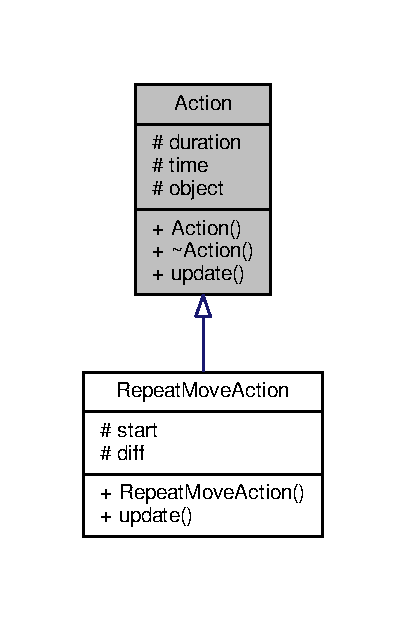
\includegraphics[width=195pt]{d2/d05/class_action__inherit__graph}
\end{center}
\end{figure}


Граф связей класса Action\+:
\nopagebreak
\begin{figure}[H]
\begin{center}
\leavevmode
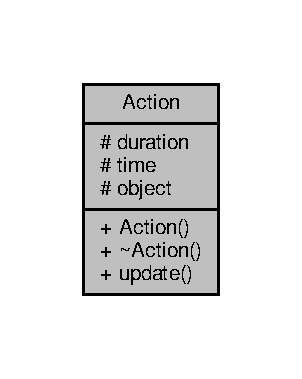
\includegraphics[width=145pt]{db/d84/class_action__coll__graph}
\end{center}
\end{figure}
\subsection*{Открытые члены}
\begin{DoxyCompactItemize}
\item 
\hyperlink{class_action_aa456764076858773c74674ba04f25bd8}{Action} (float \hyperlink{class_action_af26e528eec8ae24e9dfc1ab9d6e809a7}{duration}, weak\+\_\+ptr$<$ \hyperlink{class_scene_object}{Scene\+Object} $>$ \hyperlink{class_action_a1dfd6b0f501cce2b19d076b7d6b5aec8}{object})
\item 
virtual \hyperlink{class_action_abfc040fdc62410622a0e3835a713740f}{$\sim$\+Action} ()=default
\item 
virtual bool \hyperlink{class_action_aa6a73e716470c9b573b1afb4025b292d}{update} (float delta)=0
\end{DoxyCompactItemize}
\subsection*{Защищенные данные}
\begin{DoxyCompactItemize}
\item 
float \hyperlink{class_action_af26e528eec8ae24e9dfc1ab9d6e809a7}{duration}
\item 
float \hyperlink{class_action_a11d29bdc060c2c492d170632507c0635}{time}
\item 
weak\+\_\+ptr$<$ \hyperlink{class_scene_object}{Scene\+Object} $>$ \hyperlink{class_action_a1dfd6b0f501cce2b19d076b7d6b5aec8}{object}
\end{DoxyCompactItemize}


\subsection{Подробное описание}


См. определение в файле actions.\+h строка 9



\subsection{Конструктор(ы)}
\index{Action@{Action}!Action@{Action}}
\index{Action@{Action}!Action@{Action}}
\subsubsection[{\texorpdfstring{Action(float duration, weak\+\_\+ptr$<$ Scene\+Object $>$ object)}{Action(float duration, weak_ptr< SceneObject > object)}}]{\setlength{\rightskip}{0pt plus 5cm}Action\+::\+Action (
\begin{DoxyParamCaption}
\item[{float}]{duration, }
\item[{weak\+\_\+ptr$<$ {\bf Scene\+Object} $>$}]{object}
\end{DoxyParamCaption}
)}\hypertarget{class_action_aa456764076858773c74674ba04f25bd8}{}\label{class_action_aa456764076858773c74674ba04f25bd8}


См. определение в файле actions.\+cpp строка 3

\index{Action@{Action}!````~Action@{$\sim$\+Action}}
\index{````~Action@{$\sim$\+Action}!Action@{Action}}
\subsubsection[{\texorpdfstring{$\sim$\+Action()=default}{~Action()=default}}]{\setlength{\rightskip}{0pt plus 5cm}virtual Action\+::$\sim$\+Action (
\begin{DoxyParamCaption}
{}
\end{DoxyParamCaption}
)\hspace{0.3cm}{\ttfamily [virtual]}, {\ttfamily [default]}}\hypertarget{class_action_abfc040fdc62410622a0e3835a713740f}{}\label{class_action_abfc040fdc62410622a0e3835a713740f}


\subsection{Методы}
\index{Action@{Action}!update@{update}}
\index{update@{update}!Action@{Action}}
\subsubsection[{\texorpdfstring{update(float delta)=0}{update(float delta)=0}}]{\setlength{\rightskip}{0pt plus 5cm}virtual bool Action\+::update (
\begin{DoxyParamCaption}
\item[{float}]{delta}
\end{DoxyParamCaption}
)\hspace{0.3cm}{\ttfamily [pure virtual]}}\hypertarget{class_action_aa6a73e716470c9b573b1afb4025b292d}{}\label{class_action_aa6a73e716470c9b573b1afb4025b292d}


Замещается в \hyperlink{class_repeat_move_action_ad2a08b798e2c0ae093d1ae358c8ec3c2}{Repeat\+Move\+Action}.



\subsection{Данные класса}
\index{Action@{Action}!duration@{duration}}
\index{duration@{duration}!Action@{Action}}
\subsubsection[{\texorpdfstring{duration}{duration}}]{\setlength{\rightskip}{0pt plus 5cm}float Action\+::duration\hspace{0.3cm}{\ttfamily [protected]}}\hypertarget{class_action_af26e528eec8ae24e9dfc1ab9d6e809a7}{}\label{class_action_af26e528eec8ae24e9dfc1ab9d6e809a7}


См. определение в файле actions.\+h строка 17

\index{Action@{Action}!object@{object}}
\index{object@{object}!Action@{Action}}
\subsubsection[{\texorpdfstring{object}{object}}]{\setlength{\rightskip}{0pt plus 5cm}weak\+\_\+ptr$<${\bf Scene\+Object}$>$ Action\+::object\hspace{0.3cm}{\ttfamily [protected]}}\hypertarget{class_action_a1dfd6b0f501cce2b19d076b7d6b5aec8}{}\label{class_action_a1dfd6b0f501cce2b19d076b7d6b5aec8}


См. определение в файле actions.\+h строка 19

\index{Action@{Action}!time@{time}}
\index{time@{time}!Action@{Action}}
\subsubsection[{\texorpdfstring{time}{time}}]{\setlength{\rightskip}{0pt plus 5cm}float Action\+::time\hspace{0.3cm}{\ttfamily [protected]}}\hypertarget{class_action_a11d29bdc060c2c492d170632507c0635}{}\label{class_action_a11d29bdc060c2c492d170632507c0635}


См. определение в файле actions.\+h строка 18



Объявления и описания членов классов находятся в файлах\+:\begin{DoxyCompactItemize}
\item 
Projects/labs/course\+\_\+project\+\_\+cg/src/animation/\hyperlink{actions_8h}{actions.\+h}\item 
Projects/labs/course\+\_\+project\+\_\+cg/src/animation/\hyperlink{actions_8cpp}{actions.\+cpp}\end{DoxyCompactItemize}

\hypertarget{class_action_manager}{}\section{Класс Action\+Manager}
\label{class_action_manager}\index{Action\+Manager@{Action\+Manager}}


{\ttfamily \#include $<$actionmanager.\+h$>$}



Граф связей класса Action\+Manager\+:
\nopagebreak
\begin{figure}[H]
\begin{center}
\leavevmode
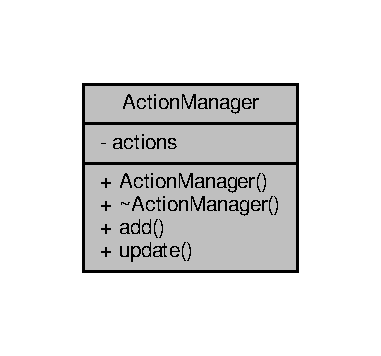
\includegraphics[width=183pt]{d3/df8/class_action_manager__coll__graph}
\end{center}
\end{figure}
\subsection*{Открытые члены}
\begin{DoxyCompactItemize}
\item 
\hyperlink{class_action_manager_a7d0c405d568795fba0c51f411e77b821}{Action\+Manager} ()
\item 
virtual \hyperlink{class_action_manager_a2fb6c58c581225959d8dfddfd386c9b3}{$\sim$\+Action\+Manager} ()=default
\item 
void \hyperlink{class_action_manager_a52f8cabe9b3fd9676e0e082ba8b741c3}{add} (unique\+\_\+ptr$<$ \hyperlink{class_action}{Action} $>$ \&\&action)
\item 
void \hyperlink{class_action_manager_a1f8ccc02cbf26b3659a08d2e7a91fdac}{update} (float delta)
\end{DoxyCompactItemize}
\subsection*{Закрытые данные}
\begin{DoxyCompactItemize}
\item 
vector$<$ unique\+\_\+ptr$<$ \hyperlink{class_action}{Action} $>$ $>$ \hyperlink{class_action_manager_a1d425cc776debdc5f32d269ee7e532bb}{actions}
\end{DoxyCompactItemize}


\subsection{Подробное описание}


См. определение в файле actionmanager.\+h строка 9



\subsection{Конструктор(ы)}
\index{Action\+Manager@{Action\+Manager}!Action\+Manager@{Action\+Manager}}
\index{Action\+Manager@{Action\+Manager}!Action\+Manager@{Action\+Manager}}
\subsubsection[{\texorpdfstring{Action\+Manager()}{ActionManager()}}]{\setlength{\rightskip}{0pt plus 5cm}Action\+Manager\+::\+Action\+Manager (
\begin{DoxyParamCaption}
{}
\end{DoxyParamCaption}
)}\hypertarget{class_action_manager_a7d0c405d568795fba0c51f411e77b821}{}\label{class_action_manager_a7d0c405d568795fba0c51f411e77b821}


См. определение в файле actionmanager.\+cpp строка 3

\index{Action\+Manager@{Action\+Manager}!````~Action\+Manager@{$\sim$\+Action\+Manager}}
\index{````~Action\+Manager@{$\sim$\+Action\+Manager}!Action\+Manager@{Action\+Manager}}
\subsubsection[{\texorpdfstring{$\sim$\+Action\+Manager()=default}{~ActionManager()=default}}]{\setlength{\rightskip}{0pt plus 5cm}virtual Action\+Manager\+::$\sim$\+Action\+Manager (
\begin{DoxyParamCaption}
{}
\end{DoxyParamCaption}
)\hspace{0.3cm}{\ttfamily [virtual]}, {\ttfamily [default]}}\hypertarget{class_action_manager_a2fb6c58c581225959d8dfddfd386c9b3}{}\label{class_action_manager_a2fb6c58c581225959d8dfddfd386c9b3}


\subsection{Методы}
\index{Action\+Manager@{Action\+Manager}!add@{add}}
\index{add@{add}!Action\+Manager@{Action\+Manager}}
\subsubsection[{\texorpdfstring{add(unique\+\_\+ptr$<$ Action $>$ \&\&action)}{add(unique_ptr< Action > &&action)}}]{\setlength{\rightskip}{0pt plus 5cm}void Action\+Manager\+::add (
\begin{DoxyParamCaption}
\item[{unique\+\_\+ptr$<$ {\bf Action} $>$ \&\&}]{action}
\end{DoxyParamCaption}
)}\hypertarget{class_action_manager_a52f8cabe9b3fd9676e0e082ba8b741c3}{}\label{class_action_manager_a52f8cabe9b3fd9676e0e082ba8b741c3}


См. определение в файле actionmanager.\+cpp строка 7

\index{Action\+Manager@{Action\+Manager}!update@{update}}
\index{update@{update}!Action\+Manager@{Action\+Manager}}
\subsubsection[{\texorpdfstring{update(float delta)}{update(float delta)}}]{\setlength{\rightskip}{0pt plus 5cm}void Action\+Manager\+::update (
\begin{DoxyParamCaption}
\item[{float}]{delta}
\end{DoxyParamCaption}
)}\hypertarget{class_action_manager_a1f8ccc02cbf26b3659a08d2e7a91fdac}{}\label{class_action_manager_a1f8ccc02cbf26b3659a08d2e7a91fdac}


См. определение в файле actionmanager.\+cpp строка 12



\subsection{Данные класса}
\index{Action\+Manager@{Action\+Manager}!actions@{actions}}
\index{actions@{actions}!Action\+Manager@{Action\+Manager}}
\subsubsection[{\texorpdfstring{actions}{actions}}]{\setlength{\rightskip}{0pt plus 5cm}vector$<$unique\+\_\+ptr$<${\bf Action}$>$ $>$ Action\+Manager\+::actions\hspace{0.3cm}{\ttfamily [private]}}\hypertarget{class_action_manager_a1d425cc776debdc5f32d269ee7e532bb}{}\label{class_action_manager_a1d425cc776debdc5f32d269ee7e532bb}


См. определение в файле actionmanager.\+h строка 20



Объявления и описания членов классов находятся в файлах\+:\begin{DoxyCompactItemize}
\item 
Projects/labs/course\+\_\+project\+\_\+cg/src/animation/\hyperlink{actionmanager_8h}{actionmanager.\+h}\item 
Projects/labs/course\+\_\+project\+\_\+cg/src/animation/\hyperlink{actionmanager_8cpp}{actionmanager.\+cpp}\end{DoxyCompactItemize}

\hypertarget{class_ambient_light}{}\section{Класс Ambient\+Light}
\label{class_ambient_light}\index{Ambient\+Light@{Ambient\+Light}}


{\ttfamily \#include $<$ambientlight.\+h$>$}



Граф наследования\+:Ambient\+Light\+:
\nopagebreak
\begin{figure}[H]
\begin{center}
\leavevmode
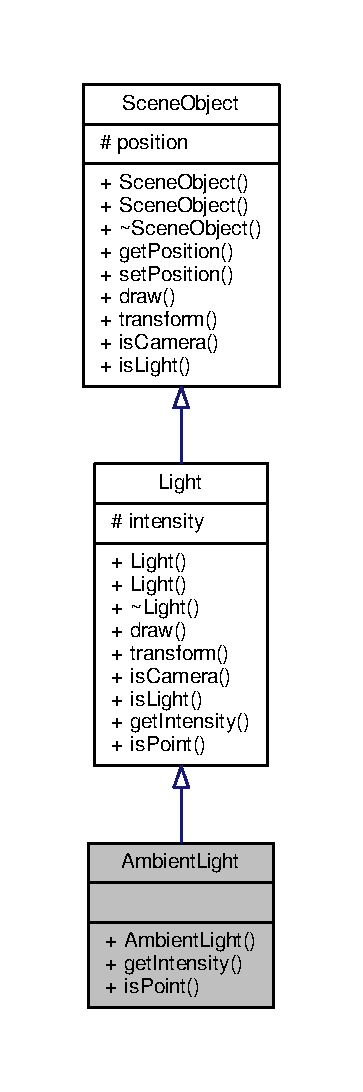
\includegraphics[width=174pt]{de/dd5/class_ambient_light__inherit__graph}
\end{center}
\end{figure}


Граф связей класса Ambient\+Light\+:
\nopagebreak
\begin{figure}[H]
\begin{center}
\leavevmode
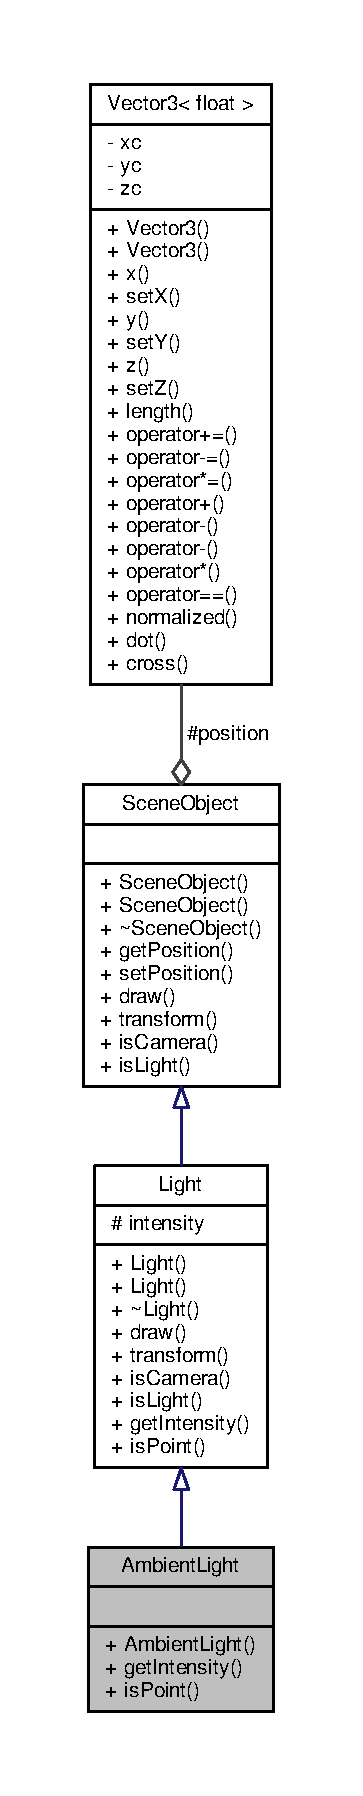
\includegraphics[height=550pt]{dd/d59/class_ambient_light__coll__graph}
\end{center}
\end{figure}
\subsection*{Открытые члены}
\begin{DoxyCompactItemize}
\item 
\hyperlink{class_ambient_light_a81a7a88347dddaf2fdec12d6d2793f8b}{Ambient\+Light} (float \hyperlink{class_light_a1071eaa556f4bb2a9345fdfba7e6f220}{intensity})
\item 
virtual \hyperlink{class_color}{Color} \hyperlink{class_ambient_light_aebbccf2534a3cbe399ccddc552d1a49d}{get\+Intensity} (const \hyperlink{vec3_8h_a221ad8ea4d9be4111628ee1ca22ee3ba}{Vec3} \&, const \hyperlink{vec3_8h_a221ad8ea4d9be4111628ee1ca22ee3ba}{Vec3} \&, const \hyperlink{vec3_8h_a221ad8ea4d9be4111628ee1ca22ee3ba}{Vec3} \&, const \hyperlink{class_color}{Color} \&ka, const \hyperlink{class_color}{Color} \&, const \hyperlink{class_color}{Color} \&, float) const override
\item 
virtual bool \hyperlink{class_ambient_light_accccb9b3c5f0a9c38dceaef386c2964a}{is\+Point} () const override
\end{DoxyCompactItemize}
\subsection*{Дополнительные унаследованные члены}


\subsection{Подробное описание}


См. определение в файле ambientlight.\+h строка 6



\subsection{Конструктор(ы)}
\index{Ambient\+Light@{Ambient\+Light}!Ambient\+Light@{Ambient\+Light}}
\index{Ambient\+Light@{Ambient\+Light}!Ambient\+Light@{Ambient\+Light}}
\subsubsection[{\texorpdfstring{Ambient\+Light(float intensity)}{AmbientLight(float intensity)}}]{\setlength{\rightskip}{0pt plus 5cm}Ambient\+Light\+::\+Ambient\+Light (
\begin{DoxyParamCaption}
\item[{float}]{intensity}
\end{DoxyParamCaption}
)}\hypertarget{class_ambient_light_a81a7a88347dddaf2fdec12d6d2793f8b}{}\label{class_ambient_light_a81a7a88347dddaf2fdec12d6d2793f8b}


См. определение в файле ambientlight.\+cpp строка 3



\subsection{Методы}
\index{Ambient\+Light@{Ambient\+Light}!get\+Intensity@{get\+Intensity}}
\index{get\+Intensity@{get\+Intensity}!Ambient\+Light@{Ambient\+Light}}
\subsubsection[{\texorpdfstring{get\+Intensity(const Vec3 \&, const Vec3 \&, const Vec3 \&, const Color \&ka, const Color \&, const Color \&, float) const override}{getIntensity(const Vec3 &, const Vec3 &, const Vec3 &, const Color &ka, const Color &, const Color &, float) const override}}]{\setlength{\rightskip}{0pt plus 5cm}{\bf Color} Ambient\+Light\+::get\+Intensity (
\begin{DoxyParamCaption}
\item[{const {\bf Vec3} \&}]{, }
\item[{const {\bf Vec3} \&}]{, }
\item[{const {\bf Vec3} \&}]{, }
\item[{const {\bf Color} \&}]{ka, }
\item[{const {\bf Color} \&}]{, }
\item[{const {\bf Color} \&}]{, }
\item[{float}]{}
\end{DoxyParamCaption}
) const\hspace{0.3cm}{\ttfamily [override]}, {\ttfamily [virtual]}}\hypertarget{class_ambient_light_aebbccf2534a3cbe399ccddc552d1a49d}{}\label{class_ambient_light_aebbccf2534a3cbe399ccddc552d1a49d}


Замещает \hyperlink{class_light_a81a8d20cdba6692644cda765aced1473}{Light}.



См. определение в файле ambientlight.\+cpp строка 9

\index{Ambient\+Light@{Ambient\+Light}!is\+Point@{is\+Point}}
\index{is\+Point@{is\+Point}!Ambient\+Light@{Ambient\+Light}}
\subsubsection[{\texorpdfstring{is\+Point() const override}{isPoint() const override}}]{\setlength{\rightskip}{0pt plus 5cm}bool Ambient\+Light\+::is\+Point (
\begin{DoxyParamCaption}
{}
\end{DoxyParamCaption}
) const\hspace{0.3cm}{\ttfamily [override]}, {\ttfamily [virtual]}}\hypertarget{class_ambient_light_accccb9b3c5f0a9c38dceaef386c2964a}{}\label{class_ambient_light_accccb9b3c5f0a9c38dceaef386c2964a}


Замещает \hyperlink{class_light_aa17c9733d1616d8631ed63640344b733}{Light}.



См. определение в файле ambientlight.\+cpp строка 16



Объявления и описания членов классов находятся в файлах\+:\begin{DoxyCompactItemize}
\item 
Projects/labs/course\+\_\+project\+\_\+cg/src/animation/\hyperlink{ambientlight_8h}{ambientlight.\+h}\item 
Projects/labs/course\+\_\+project\+\_\+cg/src/animation/\hyperlink{ambientlight_8cpp}{ambientlight.\+cpp}\end{DoxyCompactItemize}

\hypertarget{class_ambient_light_factory}{}\section{Класс Ambient\+Light\+Factory}
\label{class_ambient_light_factory}\index{Ambient\+Light\+Factory@{Ambient\+Light\+Factory}}


{\ttfamily \#include $<$sceneobjectfactory.\+h$>$}



Граф наследования\+:Ambient\+Light\+Factory\+:
\nopagebreak
\begin{figure}[H]
\begin{center}
\leavevmode
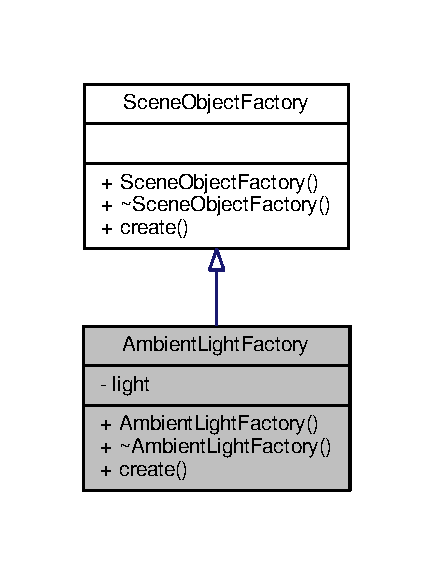
\includegraphics[width=208pt]{d9/d29/class_ambient_light_factory__inherit__graph}
\end{center}
\end{figure}


Граф связей класса Ambient\+Light\+Factory\+:
\nopagebreak
\begin{figure}[H]
\begin{center}
\leavevmode
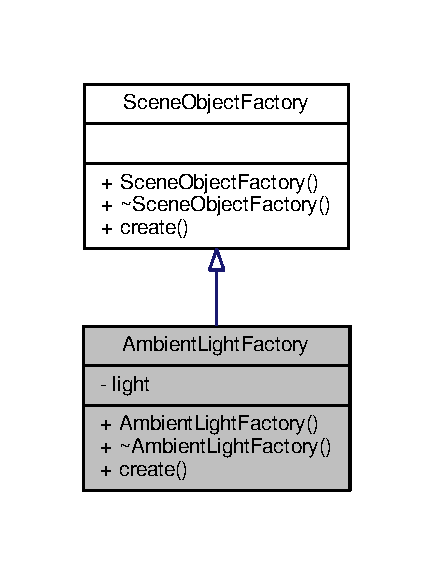
\includegraphics[width=208pt]{d3/d90/class_ambient_light_factory__coll__graph}
\end{center}
\end{figure}
\subsection*{Открытые члены}
\begin{DoxyCompactItemize}
\item 
\hyperlink{class_ambient_light_factory_ad4d095b7032ce4d9488d8ce1d845d890}{Ambient\+Light\+Factory} (float intensity)
\item 
virtual \hyperlink{class_ambient_light_factory_a160c909523b2e01f63934bc70c25f159}{$\sim$\+Ambient\+Light\+Factory} ()=default
\item 
virtual \hyperlink{sceneobject_8h_af9afe0f4fe2038e305b8b22ff495305f}{Shared\+Scene\+Object} \hyperlink{class_ambient_light_factory_a423c2ae34a9ce60c313470a4d1da0eac}{create} () override
\end{DoxyCompactItemize}
\subsection*{Закрытые данные}
\begin{DoxyCompactItemize}
\item 
std\+::unique\+\_\+ptr$<$ \hyperlink{class_ambient_light}{Ambient\+Light} $>$ \hyperlink{class_ambient_light_factory_a221bc9ca33216eece4eb9878444dbb94}{light}
\end{DoxyCompactItemize}


\subsection{Подробное описание}


См. определение в файле sceneobjectfactory.\+h строка 55



\subsection{Конструктор(ы)}
\index{Ambient\+Light\+Factory@{Ambient\+Light\+Factory}!Ambient\+Light\+Factory@{Ambient\+Light\+Factory}}
\index{Ambient\+Light\+Factory@{Ambient\+Light\+Factory}!Ambient\+Light\+Factory@{Ambient\+Light\+Factory}}
\subsubsection[{\texorpdfstring{Ambient\+Light\+Factory(float intensity)}{AmbientLightFactory(float intensity)}}]{\setlength{\rightskip}{0pt plus 5cm}Ambient\+Light\+Factory\+::\+Ambient\+Light\+Factory (
\begin{DoxyParamCaption}
\item[{float}]{intensity}
\end{DoxyParamCaption}
)}\hypertarget{class_ambient_light_factory_ad4d095b7032ce4d9488d8ce1d845d890}{}\label{class_ambient_light_factory_ad4d095b7032ce4d9488d8ce1d845d890}


См. определение в файле sceneobjectfactory.\+cpp строка 28

\index{Ambient\+Light\+Factory@{Ambient\+Light\+Factory}!````~Ambient\+Light\+Factory@{$\sim$\+Ambient\+Light\+Factory}}
\index{````~Ambient\+Light\+Factory@{$\sim$\+Ambient\+Light\+Factory}!Ambient\+Light\+Factory@{Ambient\+Light\+Factory}}
\subsubsection[{\texorpdfstring{$\sim$\+Ambient\+Light\+Factory()=default}{~AmbientLightFactory()=default}}]{\setlength{\rightskip}{0pt plus 5cm}virtual Ambient\+Light\+Factory\+::$\sim$\+Ambient\+Light\+Factory (
\begin{DoxyParamCaption}
{}
\end{DoxyParamCaption}
)\hspace{0.3cm}{\ttfamily [virtual]}, {\ttfamily [default]}}\hypertarget{class_ambient_light_factory_a160c909523b2e01f63934bc70c25f159}{}\label{class_ambient_light_factory_a160c909523b2e01f63934bc70c25f159}


\subsection{Методы}
\index{Ambient\+Light\+Factory@{Ambient\+Light\+Factory}!create@{create}}
\index{create@{create}!Ambient\+Light\+Factory@{Ambient\+Light\+Factory}}
\subsubsection[{\texorpdfstring{create() override}{create() override}}]{\setlength{\rightskip}{0pt plus 5cm}{\bf Shared\+Scene\+Object} Ambient\+Light\+Factory\+::create (
\begin{DoxyParamCaption}
{}
\end{DoxyParamCaption}
)\hspace{0.3cm}{\ttfamily [override]}, {\ttfamily [virtual]}}\hypertarget{class_ambient_light_factory_a423c2ae34a9ce60c313470a4d1da0eac}{}\label{class_ambient_light_factory_a423c2ae34a9ce60c313470a4d1da0eac}


Замещает \hyperlink{class_scene_object_factory_a9b90daaddbc34b747c072f770bc6b993}{Scene\+Object\+Factory}.



См. определение в файле sceneobjectfactory.\+cpp строка 33



\subsection{Данные класса}
\index{Ambient\+Light\+Factory@{Ambient\+Light\+Factory}!light@{light}}
\index{light@{light}!Ambient\+Light\+Factory@{Ambient\+Light\+Factory}}
\subsubsection[{\texorpdfstring{light}{light}}]{\setlength{\rightskip}{0pt plus 5cm}std\+::unique\+\_\+ptr$<${\bf Ambient\+Light}$>$ Ambient\+Light\+Factory\+::light\hspace{0.3cm}{\ttfamily [private]}}\hypertarget{class_ambient_light_factory_a221bc9ca33216eece4eb9878444dbb94}{}\label{class_ambient_light_factory_a221bc9ca33216eece4eb9878444dbb94}


См. определение в файле sceneobjectfactory.\+h строка 63



Объявления и описания членов классов находятся в файлах\+:\begin{DoxyCompactItemize}
\item 
Projects/labs/course\+\_\+project\+\_\+cg/src/animation/\hyperlink{sceneobjectfactory_8h}{sceneobjectfactory.\+h}\item 
Projects/labs/course\+\_\+project\+\_\+cg/src/animation/\hyperlink{sceneobjectfactory_8cpp}{sceneobjectfactory.\+cpp}\end{DoxyCompactItemize}

\hypertarget{class_animation_window}{}\section{Класс Animation\+Window}
\label{class_animation_window}\index{Animation\+Window@{Animation\+Window}}


{\ttfamily \#include $<$animationwindow.\+h$>$}



Граф наследования\+:Animation\+Window\+:
\nopagebreak
\begin{figure}[H]
\begin{center}
\leavevmode
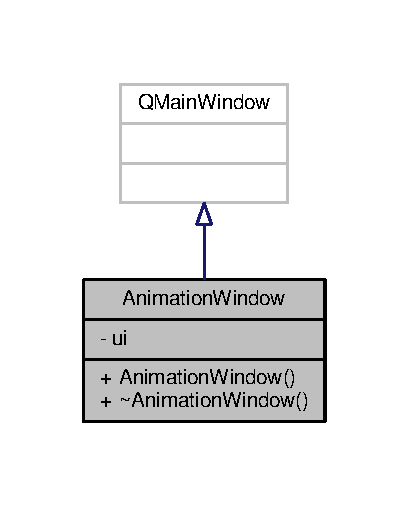
\includegraphics[width=196pt]{d4/d61/class_animation_window__inherit__graph}
\end{center}
\end{figure}


Граф связей класса Animation\+Window\+:
\nopagebreak
\begin{figure}[H]
\begin{center}
\leavevmode
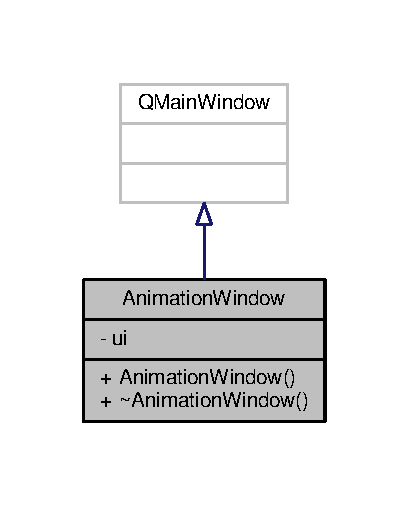
\includegraphics[width=196pt]{da/d3c/class_animation_window__coll__graph}
\end{center}
\end{figure}
\subsection*{Открытые члены}
\begin{DoxyCompactItemize}
\item 
\hyperlink{class_animation_window_a3473a525d4aa738d2569731e26b95570}{Animation\+Window} (Q\+Widget $\ast$parent=0)
\item 
\hyperlink{class_animation_window_a2570db590e94da377cdcfa7088240ab2}{$\sim$\+Animation\+Window} ()
\end{DoxyCompactItemize}
\subsection*{Закрытые данные}
\begin{DoxyCompactItemize}
\item 
Ui\+::\+Animation\+Window $\ast$ \hyperlink{class_animation_window_a1db782b4d22aec2376c6db4431c77a80}{ui}
\end{DoxyCompactItemize}


\subsection{Подробное описание}


См. определение в файле animationwindow.\+h строка 10



\subsection{Конструктор(ы)}
\index{Animation\+Window@{Animation\+Window}!Animation\+Window@{Animation\+Window}}
\index{Animation\+Window@{Animation\+Window}!Animation\+Window@{Animation\+Window}}
\subsubsection[{\texorpdfstring{Animation\+Window(\+Q\+Widget $\ast$parent=0)}{AnimationWindow(QWidget *parent=0)}}]{\setlength{\rightskip}{0pt plus 5cm}Animation\+Window\+::\+Animation\+Window (
\begin{DoxyParamCaption}
\item[{Q\+Widget $\ast$}]{parent = {\ttfamily 0}}
\end{DoxyParamCaption}
)\hspace{0.3cm}{\ttfamily [explicit]}}\hypertarget{class_animation_window_a3473a525d4aa738d2569731e26b95570}{}\label{class_animation_window_a3473a525d4aa738d2569731e26b95570}


См. определение в файле animationwindow.\+cpp строка 4

\index{Animation\+Window@{Animation\+Window}!````~Animation\+Window@{$\sim$\+Animation\+Window}}
\index{````~Animation\+Window@{$\sim$\+Animation\+Window}!Animation\+Window@{Animation\+Window}}
\subsubsection[{\texorpdfstring{$\sim$\+Animation\+Window()}{~AnimationWindow()}}]{\setlength{\rightskip}{0pt plus 5cm}Animation\+Window\+::$\sim$\+Animation\+Window (
\begin{DoxyParamCaption}
{}
\end{DoxyParamCaption}
)}\hypertarget{class_animation_window_a2570db590e94da377cdcfa7088240ab2}{}\label{class_animation_window_a2570db590e94da377cdcfa7088240ab2}


См. определение в файле animationwindow.\+cpp строка 11



\subsection{Данные класса}
\index{Animation\+Window@{Animation\+Window}!ui@{ui}}
\index{ui@{ui}!Animation\+Window@{Animation\+Window}}
\subsubsection[{\texorpdfstring{ui}{ui}}]{\setlength{\rightskip}{0pt plus 5cm}Ui\+::\+Animation\+Window$\ast$ Animation\+Window\+::ui\hspace{0.3cm}{\ttfamily [private]}}\hypertarget{class_animation_window_a1db782b4d22aec2376c6db4431c77a80}{}\label{class_animation_window_a1db782b4d22aec2376c6db4431c77a80}


См. определение в файле animationwindow.\+h строка 19



Объявления и описания членов классов находятся в файлах\+:\begin{DoxyCompactItemize}
\item 
Projects/labs/course\+\_\+project\+\_\+cg/src/\hyperlink{animationwindow_8h}{animationwindow.\+h}\item 
Projects/labs/course\+\_\+project\+\_\+cg/src/\hyperlink{animationwindow_8cpp}{animationwindow.\+cpp}\end{DoxyCompactItemize}

\hypertarget{class_blur}{}\section{Класс Blur}
\label{class_blur}\index{Blur@{Blur}}


{\ttfamily \#include $<$blur.\+h$>$}



Граф наследования\+:Blur\+:
\nopagebreak
\begin{figure}[H]
\begin{center}
\leavevmode
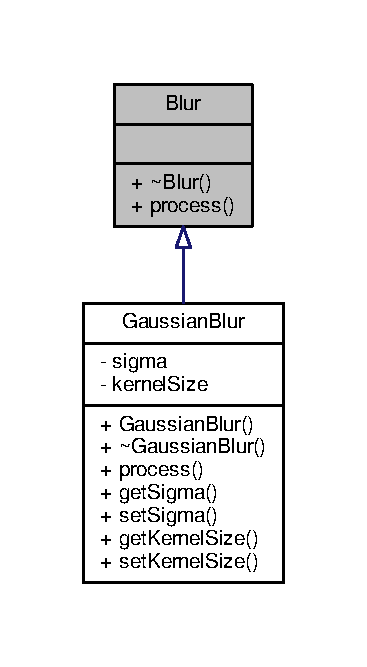
\includegraphics[width=176pt]{d9/d38/class_blur__inherit__graph}
\end{center}
\end{figure}


Граф связей класса Blur\+:
\nopagebreak
\begin{figure}[H]
\begin{center}
\leavevmode
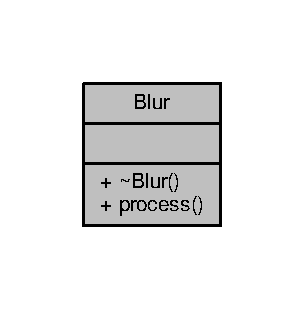
\includegraphics[width=146pt]{db/d4b/class_blur__coll__graph}
\end{center}
\end{figure}
\subsection*{Открытые члены}
\begin{DoxyCompactItemize}
\item 
virtual \hyperlink{class_blur_a6b1d2a771f096d933b72f4dff5f07d2d}{$\sim$\+Blur} ()
\item 
virtual void \hyperlink{class_blur_a675fd2caa4a262e8140bdff64912bab4}{process} (\hyperlink{class_image}{Image} \&image)=0
\end{DoxyCompactItemize}


\subsection{Подробное описание}


См. определение в файле blur.\+h строка 6



\subsection{Конструктор(ы)}
\index{Blur@{Blur}!````~Blur@{$\sim$\+Blur}}
\index{````~Blur@{$\sim$\+Blur}!Blur@{Blur}}
\subsubsection[{\texorpdfstring{$\sim$\+Blur()}{~Blur()}}]{\setlength{\rightskip}{0pt plus 5cm}Blur\+::$\sim$\+Blur (
\begin{DoxyParamCaption}
{}
\end{DoxyParamCaption}
)\hspace{0.3cm}{\ttfamily [virtual]}}\hypertarget{class_blur_a6b1d2a771f096d933b72f4dff5f07d2d}{}\label{class_blur_a6b1d2a771f096d933b72f4dff5f07d2d}


См. определение в файле blur.\+cpp строка 4



\subsection{Методы}
\index{Blur@{Blur}!process@{process}}
\index{process@{process}!Blur@{Blur}}
\subsubsection[{\texorpdfstring{process(\+Image \&image)=0}{process(Image &image)=0}}]{\setlength{\rightskip}{0pt plus 5cm}virtual void Blur\+::process (
\begin{DoxyParamCaption}
\item[{{\bf Image} \&}]{image}
\end{DoxyParamCaption}
)\hspace{0.3cm}{\ttfamily [pure virtual]}}\hypertarget{class_blur_a675fd2caa4a262e8140bdff64912bab4}{}\label{class_blur_a675fd2caa4a262e8140bdff64912bab4}


Замещается в \hyperlink{class_gaussian_blur_a6af6684bdf5e86e5c9a79fe1f3a8c183}{Gaussian\+Blur}.



Объявления и описания членов классов находятся в файлах\+:\begin{DoxyCompactItemize}
\item 
Projects/labs/course\+\_\+project\+\_\+cg/src/algorithm/blur/\hyperlink{blur_8h}{blur.\+h}\item 
Projects/labs/course\+\_\+project\+\_\+cg/src/algorithm/blur/\hyperlink{blur_8cpp}{blur.\+cpp}\end{DoxyCompactItemize}

\hypertarget{class_camera}{}\section{Класс Camera}
\label{class_camera}\index{Camera@{Camera}}


{\ttfamily \#include $<$camera.\+h$>$}



Граф наследования\+:Camera\+:
\nopagebreak
\begin{figure}[H]
\begin{center}
\leavevmode
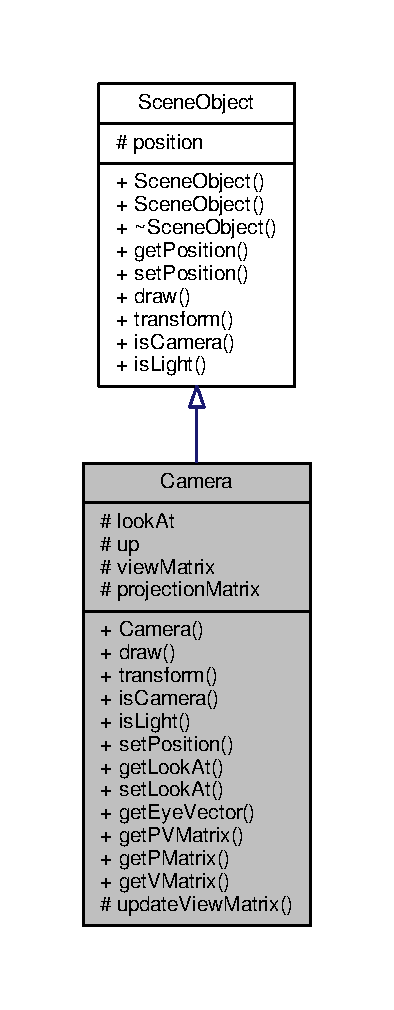
\includegraphics[width=189pt]{db/d34/class_camera__inherit__graph}
\end{center}
\end{figure}


Граф связей класса Camera\+:
\nopagebreak
\begin{figure}[H]
\begin{center}
\leavevmode
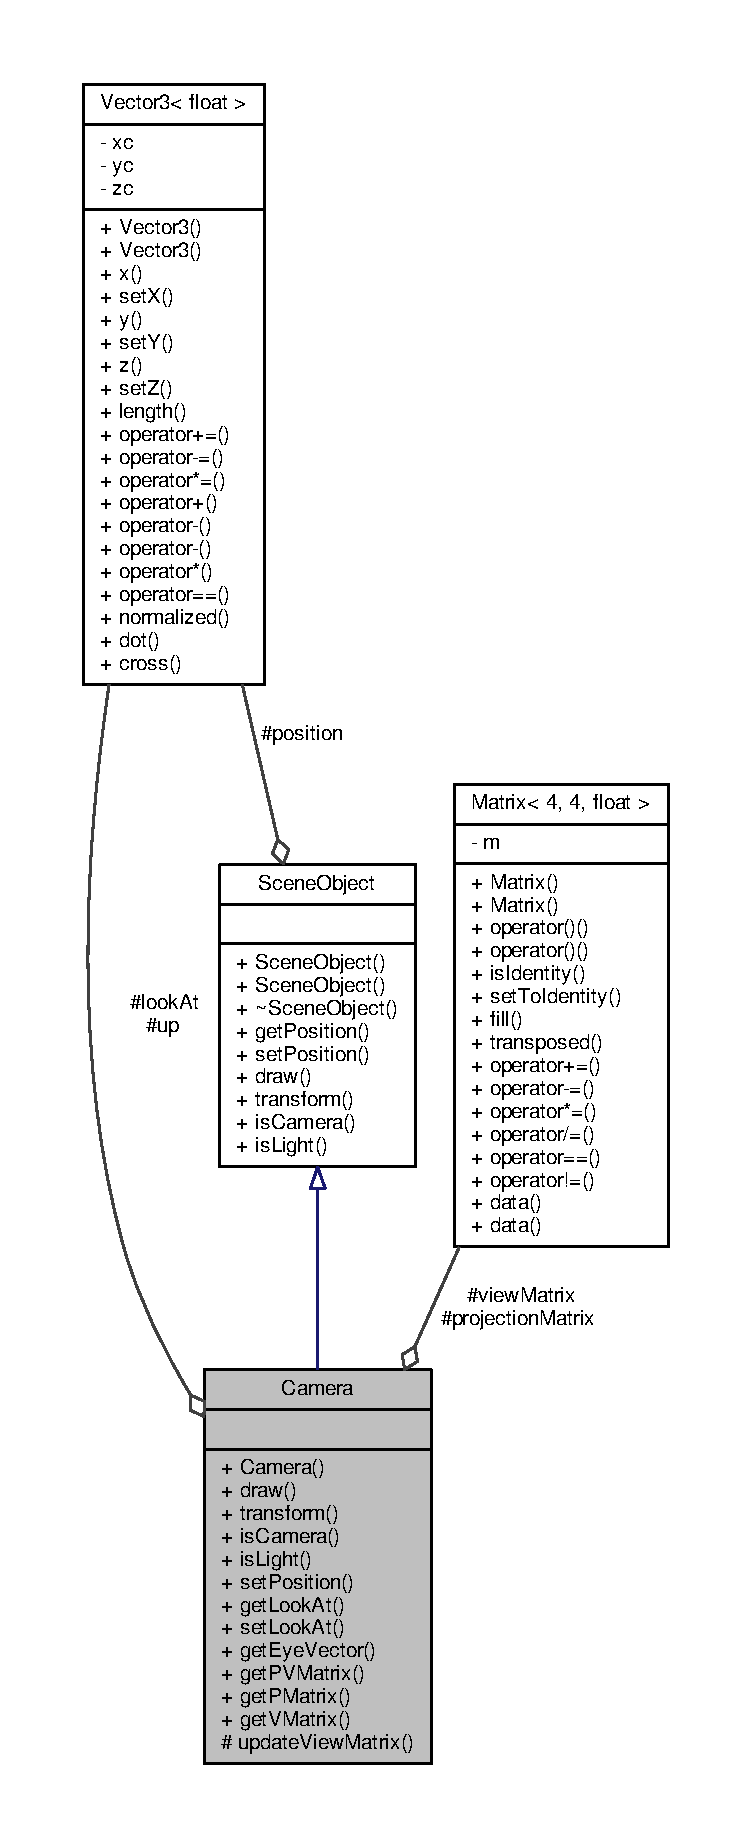
\includegraphics[height=550pt]{d0/dcb/class_camera__coll__graph}
\end{center}
\end{figure}
\subsection*{Открытые члены}
\begin{DoxyCompactItemize}
\item 
\hyperlink{class_camera_a2f7d35911a4dcf218a0ef901cc0906dc}{Camera} (const \hyperlink{vec3_8h_a221ad8ea4d9be4111628ee1ca22ee3ba}{Vec3} \&\hyperlink{class_scene_object_af190cdf9b9449f96f73d836848ce4ad3}{position}, const \hyperlink{vec3_8h_a221ad8ea4d9be4111628ee1ca22ee3ba}{Vec3} \&\hyperlink{class_camera_a7aa44d09547fc7407002dc32b1891207}{look\+At}, const \hyperlink{vec3_8h_a221ad8ea4d9be4111628ee1ca22ee3ba}{Vec3} \&\hyperlink{class_camera_a4473532c8bbceefb503a5a7195044bfe}{up}, const \hyperlink{matrix_8h_a077dce9756976f552e5703c34475d5e3}{Mat4} \&projection)
\item 
virtual void \hyperlink{class_camera_a5c5155e999ea54c0385461de3ca0b95a}{draw} (std\+::unique\+\_\+ptr$<$ \hyperlink{class_renderer}{Renderer} $>$ \&) override
\item 
virtual void \hyperlink{class_camera_a76d8a9057211e4935405040d8fa154f6}{transform} (\hyperlink{class_transformation}{Transformation} \&transformation) override
\item 
virtual bool \hyperlink{class_camera_a629ebafac4f86f952dad42a0087c344c}{is\+Camera} () override
\item 
virtual bool \hyperlink{class_camera_a7209dc5149f4b8af2ed9e8b6297f6c41}{is\+Light} () override
\item 
virtual void \hyperlink{class_camera_a1ba2c3600a8a0f6e231ad9564bdb7359}{set\+Position} (const \hyperlink{vec3_8h_a221ad8ea4d9be4111628ee1ca22ee3ba}{Vec3} \&value) override
\item 
virtual const \hyperlink{vec3_8h_a221ad8ea4d9be4111628ee1ca22ee3ba}{Vec3} \& \hyperlink{class_camera_a318614134ed9e5182954daaceb17ca47}{get\+Look\+At} ()
\item 
virtual void \hyperlink{class_camera_abd0ac1ec8cc6c5ca79798fc61aa4a1fa}{set\+Look\+At} (const \hyperlink{vec3_8h_a221ad8ea4d9be4111628ee1ca22ee3ba}{Vec3} \&target)
\item 
virtual \hyperlink{vec3_8h_a221ad8ea4d9be4111628ee1ca22ee3ba}{Vec3} \hyperlink{class_camera_a49e96c7af94f85b1297fb4184c99fa28}{get\+Eye\+Vector} ()
\item 
virtual \hyperlink{matrix_8h_a077dce9756976f552e5703c34475d5e3}{Mat4} \hyperlink{class_camera_a081e90588c62b55623f22d0477082924}{get\+P\+V\+Matrix} ()
\item 
virtual const \hyperlink{matrix_8h_a077dce9756976f552e5703c34475d5e3}{Mat4} \& \hyperlink{class_camera_a0baac3a162f4e3507a5c35c97a2c4236}{get\+P\+Matrix} () const 
\item 
virtual const \hyperlink{matrix_8h_a077dce9756976f552e5703c34475d5e3}{Mat4} \& \hyperlink{class_camera_ac9ca414b8f610584b90486938131aa1e}{get\+V\+Matrix} () const 
\end{DoxyCompactItemize}
\subsection*{Защищенные члены}
\begin{DoxyCompactItemize}
\item 
void \hyperlink{class_camera_a8fe5c71a390571a861ad8afd99dfdea3}{update\+View\+Matrix} ()
\end{DoxyCompactItemize}
\subsection*{Защищенные данные}
\begin{DoxyCompactItemize}
\item 
\hyperlink{vec3_8h_a221ad8ea4d9be4111628ee1ca22ee3ba}{Vec3} \hyperlink{class_camera_a7aa44d09547fc7407002dc32b1891207}{look\+At}
\item 
\hyperlink{vec3_8h_a221ad8ea4d9be4111628ee1ca22ee3ba}{Vec3} \hyperlink{class_camera_a4473532c8bbceefb503a5a7195044bfe}{up}
\item 
\hyperlink{matrix_8h_a077dce9756976f552e5703c34475d5e3}{Mat4} \hyperlink{class_camera_a9e4efa2b0bb97699cda8904309873aa9}{view\+Matrix}
\item 
\hyperlink{matrix_8h_a077dce9756976f552e5703c34475d5e3}{Mat4} \hyperlink{class_camera_a33e328413d91278d44953ccb0adef3ce}{projection\+Matrix}
\end{DoxyCompactItemize}


\subsection{Подробное описание}


См. определение в файле camera.\+h строка 7



\subsection{Конструктор(ы)}
\index{Camera@{Camera}!Camera@{Camera}}
\index{Camera@{Camera}!Camera@{Camera}}
\subsubsection[{\texorpdfstring{Camera(const Vec3 \&position, const Vec3 \&look\+At, const Vec3 \&up, const Mat4 \&projection)}{Camera(const Vec3 &position, const Vec3 &lookAt, const Vec3 &up, const Mat4 &projection)}}]{\setlength{\rightskip}{0pt plus 5cm}Camera\+::\+Camera (
\begin{DoxyParamCaption}
\item[{const {\bf Vec3} \&}]{position, }
\item[{const {\bf Vec3} \&}]{look\+At, }
\item[{const {\bf Vec3} \&}]{up, }
\item[{const {\bf Mat4} \&}]{projection}
\end{DoxyParamCaption}
)}\hypertarget{class_camera_a2f7d35911a4dcf218a0ef901cc0906dc}{}\label{class_camera_a2f7d35911a4dcf218a0ef901cc0906dc}


См. определение в файле camera.\+cpp строка 6



\subsection{Методы}
\index{Camera@{Camera}!draw@{draw}}
\index{draw@{draw}!Camera@{Camera}}
\subsubsection[{\texorpdfstring{draw(std\+::unique\+\_\+ptr$<$ Renderer $>$ \&) override}{draw(std::unique_ptr< Renderer > &) override}}]{\setlength{\rightskip}{0pt plus 5cm}void Camera\+::draw (
\begin{DoxyParamCaption}
\item[{std\+::unique\+\_\+ptr$<$ {\bf Renderer} $>$ \&}]{}
\end{DoxyParamCaption}
)\hspace{0.3cm}{\ttfamily [override]}, {\ttfamily [virtual]}}\hypertarget{class_camera_a5c5155e999ea54c0385461de3ca0b95a}{}\label{class_camera_a5c5155e999ea54c0385461de3ca0b95a}


Замещает \hyperlink{class_scene_object_adc906ce4e4a896a351949ccabfd44016}{Scene\+Object}.



См. определение в файле camera.\+cpp строка 17

\index{Camera@{Camera}!get\+Eye\+Vector@{get\+Eye\+Vector}}
\index{get\+Eye\+Vector@{get\+Eye\+Vector}!Camera@{Camera}}
\subsubsection[{\texorpdfstring{get\+Eye\+Vector()}{getEyeVector()}}]{\setlength{\rightskip}{0pt plus 5cm}{\bf Vec3} Camera\+::get\+Eye\+Vector (
\begin{DoxyParamCaption}
{}
\end{DoxyParamCaption}
)\hspace{0.3cm}{\ttfamily [virtual]}}\hypertarget{class_camera_a49e96c7af94f85b1297fb4184c99fa28}{}\label{class_camera_a49e96c7af94f85b1297fb4184c99fa28}


См. определение в файле camera.\+cpp строка 44

\index{Camera@{Camera}!get\+Look\+At@{get\+Look\+At}}
\index{get\+Look\+At@{get\+Look\+At}!Camera@{Camera}}
\subsubsection[{\texorpdfstring{get\+Look\+At()}{getLookAt()}}]{\setlength{\rightskip}{0pt plus 5cm}const {\bf Vec3} \& Camera\+::get\+Look\+At (
\begin{DoxyParamCaption}
{}
\end{DoxyParamCaption}
)\hspace{0.3cm}{\ttfamily [virtual]}}\hypertarget{class_camera_a318614134ed9e5182954daaceb17ca47}{}\label{class_camera_a318614134ed9e5182954daaceb17ca47}


См. определение в файле camera.\+cpp строка 76

\index{Camera@{Camera}!get\+P\+Matrix@{get\+P\+Matrix}}
\index{get\+P\+Matrix@{get\+P\+Matrix}!Camera@{Camera}}
\subsubsection[{\texorpdfstring{get\+P\+Matrix() const }{getPMatrix() const }}]{\setlength{\rightskip}{0pt plus 5cm}const {\bf Mat4} \& Camera\+::get\+P\+Matrix (
\begin{DoxyParamCaption}
{}
\end{DoxyParamCaption}
) const\hspace{0.3cm}{\ttfamily [virtual]}}\hypertarget{class_camera_a0baac3a162f4e3507a5c35c97a2c4236}{}\label{class_camera_a0baac3a162f4e3507a5c35c97a2c4236}


См. определение в файле camera.\+cpp строка 54

\index{Camera@{Camera}!get\+P\+V\+Matrix@{get\+P\+V\+Matrix}}
\index{get\+P\+V\+Matrix@{get\+P\+V\+Matrix}!Camera@{Camera}}
\subsubsection[{\texorpdfstring{get\+P\+V\+Matrix()}{getPVMatrix()}}]{\setlength{\rightskip}{0pt plus 5cm}{\bf Mat4} Camera\+::get\+P\+V\+Matrix (
\begin{DoxyParamCaption}
{}
\end{DoxyParamCaption}
)\hspace{0.3cm}{\ttfamily [virtual]}}\hypertarget{class_camera_a081e90588c62b55623f22d0477082924}{}\label{class_camera_a081e90588c62b55623f22d0477082924}


См. определение в файле camera.\+cpp строка 49

\index{Camera@{Camera}!get\+V\+Matrix@{get\+V\+Matrix}}
\index{get\+V\+Matrix@{get\+V\+Matrix}!Camera@{Camera}}
\subsubsection[{\texorpdfstring{get\+V\+Matrix() const }{getVMatrix() const }}]{\setlength{\rightskip}{0pt plus 5cm}const {\bf Mat4} \& Camera\+::get\+V\+Matrix (
\begin{DoxyParamCaption}
{}
\end{DoxyParamCaption}
) const\hspace{0.3cm}{\ttfamily [virtual]}}\hypertarget{class_camera_ac9ca414b8f610584b90486938131aa1e}{}\label{class_camera_ac9ca414b8f610584b90486938131aa1e}


См. определение в файле camera.\+cpp строка 59

\index{Camera@{Camera}!is\+Camera@{is\+Camera}}
\index{is\+Camera@{is\+Camera}!Camera@{Camera}}
\subsubsection[{\texorpdfstring{is\+Camera() override}{isCamera() override}}]{\setlength{\rightskip}{0pt plus 5cm}bool Camera\+::is\+Camera (
\begin{DoxyParamCaption}
{}
\end{DoxyParamCaption}
)\hspace{0.3cm}{\ttfamily [override]}, {\ttfamily [virtual]}}\hypertarget{class_camera_a629ebafac4f86f952dad42a0087c344c}{}\label{class_camera_a629ebafac4f86f952dad42a0087c344c}


Замещает \hyperlink{class_scene_object_a6d7cb8b9a2c29f38fd039731e83167f4}{Scene\+Object}.



См. определение в файле camera.\+cpp строка 28

\index{Camera@{Camera}!is\+Light@{is\+Light}}
\index{is\+Light@{is\+Light}!Camera@{Camera}}
\subsubsection[{\texorpdfstring{is\+Light() override}{isLight() override}}]{\setlength{\rightskip}{0pt plus 5cm}bool Camera\+::is\+Light (
\begin{DoxyParamCaption}
{}
\end{DoxyParamCaption}
)\hspace{0.3cm}{\ttfamily [override]}, {\ttfamily [virtual]}}\hypertarget{class_camera_a7209dc5149f4b8af2ed9e8b6297f6c41}{}\label{class_camera_a7209dc5149f4b8af2ed9e8b6297f6c41}


Замещает \hyperlink{class_scene_object_a9c5b006b8a0e457634f15c19eb51ca73}{Scene\+Object}.



См. определение в файле camera.\+cpp строка 33

\index{Camera@{Camera}!set\+Look\+At@{set\+Look\+At}}
\index{set\+Look\+At@{set\+Look\+At}!Camera@{Camera}}
\subsubsection[{\texorpdfstring{set\+Look\+At(const Vec3 \&target)}{setLookAt(const Vec3 &target)}}]{\setlength{\rightskip}{0pt plus 5cm}void Camera\+::set\+Look\+At (
\begin{DoxyParamCaption}
\item[{const {\bf Vec3} \&}]{target}
\end{DoxyParamCaption}
)\hspace{0.3cm}{\ttfamily [virtual]}}\hypertarget{class_camera_abd0ac1ec8cc6c5ca79798fc61aa4a1fa}{}\label{class_camera_abd0ac1ec8cc6c5ca79798fc61aa4a1fa}


См. определение в файле camera.\+cpp строка 38

\index{Camera@{Camera}!set\+Position@{set\+Position}}
\index{set\+Position@{set\+Position}!Camera@{Camera}}
\subsubsection[{\texorpdfstring{set\+Position(const Vec3 \&value) override}{setPosition(const Vec3 &value) override}}]{\setlength{\rightskip}{0pt plus 5cm}void Camera\+::set\+Position (
\begin{DoxyParamCaption}
\item[{const {\bf Vec3} \&}]{value}
\end{DoxyParamCaption}
)\hspace{0.3cm}{\ttfamily [override]}, {\ttfamily [virtual]}}\hypertarget{class_camera_a1ba2c3600a8a0f6e231ad9564bdb7359}{}\label{class_camera_a1ba2c3600a8a0f6e231ad9564bdb7359}


Переопределяет метод предка \hyperlink{class_scene_object_ae0e79b1773e3e3357d1dcf302463e46a}{Scene\+Object}.



См. определение в файле camera.\+cpp строка 70

\index{Camera@{Camera}!transform@{transform}}
\index{transform@{transform}!Camera@{Camera}}
\subsubsection[{\texorpdfstring{transform(\+Transformation \&transformation) override}{transform(Transformation &transformation) override}}]{\setlength{\rightskip}{0pt plus 5cm}void Camera\+::transform (
\begin{DoxyParamCaption}
\item[{{\bf Transformation} \&}]{transformation}
\end{DoxyParamCaption}
)\hspace{0.3cm}{\ttfamily [override]}, {\ttfamily [virtual]}}\hypertarget{class_camera_a76d8a9057211e4935405040d8fa154f6}{}\label{class_camera_a76d8a9057211e4935405040d8fa154f6}


Замещает \hyperlink{class_scene_object_a1b8a4b90f1200f1cd025d95964d43630}{Scene\+Object}.



См. определение в файле camera.\+cpp строка 22

\index{Camera@{Camera}!update\+View\+Matrix@{update\+View\+Matrix}}
\index{update\+View\+Matrix@{update\+View\+Matrix}!Camera@{Camera}}
\subsubsection[{\texorpdfstring{update\+View\+Matrix()}{updateViewMatrix()}}]{\setlength{\rightskip}{0pt plus 5cm}void Camera\+::update\+View\+Matrix (
\begin{DoxyParamCaption}
{}
\end{DoxyParamCaption}
)\hspace{0.3cm}{\ttfamily [protected]}}\hypertarget{class_camera_a8fe5c71a390571a861ad8afd99dfdea3}{}\label{class_camera_a8fe5c71a390571a861ad8afd99dfdea3}


См. определение в файле camera.\+cpp строка 64



\subsection{Данные класса}
\index{Camera@{Camera}!look\+At@{look\+At}}
\index{look\+At@{look\+At}!Camera@{Camera}}
\subsubsection[{\texorpdfstring{look\+At}{lookAt}}]{\setlength{\rightskip}{0pt plus 5cm}{\bf Vec3} Camera\+::look\+At\hspace{0.3cm}{\ttfamily [protected]}}\hypertarget{class_camera_a7aa44d09547fc7407002dc32b1891207}{}\label{class_camera_a7aa44d09547fc7407002dc32b1891207}


См. определение в файле camera.\+h строка 30

\index{Camera@{Camera}!projection\+Matrix@{projection\+Matrix}}
\index{projection\+Matrix@{projection\+Matrix}!Camera@{Camera}}
\subsubsection[{\texorpdfstring{projection\+Matrix}{projectionMatrix}}]{\setlength{\rightskip}{0pt plus 5cm}{\bf Mat4} Camera\+::projection\+Matrix\hspace{0.3cm}{\ttfamily [protected]}}\hypertarget{class_camera_a33e328413d91278d44953ccb0adef3ce}{}\label{class_camera_a33e328413d91278d44953ccb0adef3ce}


См. определение в файле camera.\+h строка 33

\index{Camera@{Camera}!up@{up}}
\index{up@{up}!Camera@{Camera}}
\subsubsection[{\texorpdfstring{up}{up}}]{\setlength{\rightskip}{0pt plus 5cm}{\bf Vec3} Camera\+::up\hspace{0.3cm}{\ttfamily [protected]}}\hypertarget{class_camera_a4473532c8bbceefb503a5a7195044bfe}{}\label{class_camera_a4473532c8bbceefb503a5a7195044bfe}


См. определение в файле camera.\+h строка 31

\index{Camera@{Camera}!view\+Matrix@{view\+Matrix}}
\index{view\+Matrix@{view\+Matrix}!Camera@{Camera}}
\subsubsection[{\texorpdfstring{view\+Matrix}{viewMatrix}}]{\setlength{\rightskip}{0pt plus 5cm}{\bf Mat4} Camera\+::view\+Matrix\hspace{0.3cm}{\ttfamily [protected]}}\hypertarget{class_camera_a9e4efa2b0bb97699cda8904309873aa9}{}\label{class_camera_a9e4efa2b0bb97699cda8904309873aa9}


См. определение в файле camera.\+h строка 32



Объявления и описания членов классов находятся в файлах\+:\begin{DoxyCompactItemize}
\item 
Projects/labs/course\+\_\+project\+\_\+cg/src/animation/\hyperlink{camera_8h}{camera.\+h}\item 
Projects/labs/course\+\_\+project\+\_\+cg/src/animation/\hyperlink{camera_8cpp}{camera.\+cpp}\end{DoxyCompactItemize}

\hypertarget{class_camera_factory}{}\section{Класс Camera\+Factory}
\label{class_camera_factory}\index{Camera\+Factory@{Camera\+Factory}}


{\ttfamily \#include $<$sceneobjectfactory.\+h$>$}



Граф наследования\+:Camera\+Factory\+:
\nopagebreak
\begin{figure}[H]
\begin{center}
\leavevmode
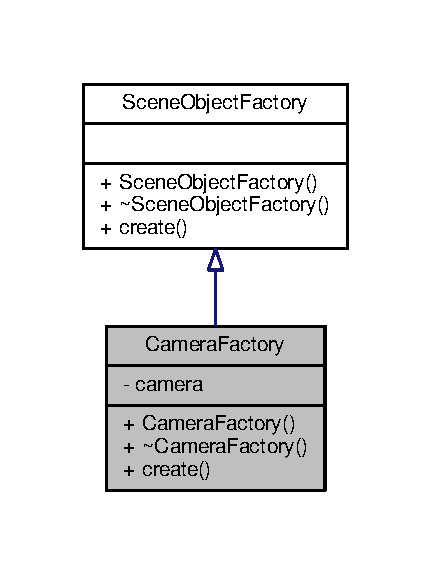
\includegraphics[width=207pt]{dc/db7/class_camera_factory__inherit__graph}
\end{center}
\end{figure}


Граф связей класса Camera\+Factory\+:
\nopagebreak
\begin{figure}[H]
\begin{center}
\leavevmode
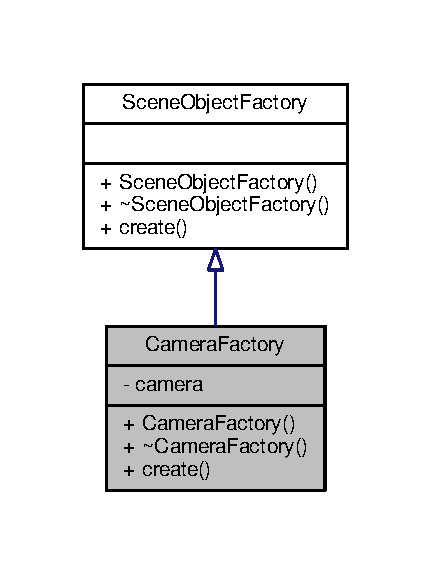
\includegraphics[width=207pt]{da/d5f/class_camera_factory__coll__graph}
\end{center}
\end{figure}
\subsection*{Классы}
\begin{DoxyCompactItemize}
\item 
struct \hyperlink{struct_camera_factory_1_1_perspective_data}{Perspective\+Data}
\end{DoxyCompactItemize}
\subsection*{Открытые члены}
\begin{DoxyCompactItemize}
\item 
\hyperlink{class_camera_factory_a73bf5c839340ca2a94ce52a1c400d231}{Camera\+Factory} (const \hyperlink{vec3_8h_a221ad8ea4d9be4111628ee1ca22ee3ba}{Vec3} \&position, const \hyperlink{vec3_8h_a221ad8ea4d9be4111628ee1ca22ee3ba}{Vec3} \&look\+At, const \hyperlink{vec3_8h_a221ad8ea4d9be4111628ee1ca22ee3ba}{Vec3} \&up, const \hyperlink{struct_camera_factory_1_1_perspective_data}{Perspective\+Data} \&data)
\item 
virtual \hyperlink{class_camera_factory_ab63fa4fcfc787465aa1b2d5bf03e9a4d}{$\sim$\+Camera\+Factory} ()=default
\item 
virtual \hyperlink{sceneobject_8h_af9afe0f4fe2038e305b8b22ff495305f}{Shared\+Scene\+Object} \hyperlink{class_camera_factory_a7a105ab24599d2d48fc03f40a28a1492}{create} () override
\end{DoxyCompactItemize}
\subsection*{Закрытые данные}
\begin{DoxyCompactItemize}
\item 
std\+::unique\+\_\+ptr$<$ \hyperlink{class_camera}{Camera} $>$ \hyperlink{class_camera_factory_ad1e2114f133f8489e790a4f42b377de3}{camera}
\end{DoxyCompactItemize}


\subsection{Подробное описание}


См. определение в файле sceneobjectfactory.\+h строка 21



\subsection{Конструктор(ы)}
\index{Camera\+Factory@{Camera\+Factory}!Camera\+Factory@{Camera\+Factory}}
\index{Camera\+Factory@{Camera\+Factory}!Camera\+Factory@{Camera\+Factory}}
\subsubsection[{\texorpdfstring{Camera\+Factory(const Vec3 \&position, const Vec3 \&look\+At, const Vec3 \&up, const Perspective\+Data \&data)}{CameraFactory(const Vec3 &position, const Vec3 &lookAt, const Vec3 &up, const PerspectiveData &data)}}]{\setlength{\rightskip}{0pt plus 5cm}Camera\+Factory\+::\+Camera\+Factory (
\begin{DoxyParamCaption}
\item[{const {\bf Vec3} \&}]{position, }
\item[{const {\bf Vec3} \&}]{look\+At, }
\item[{const {\bf Vec3} \&}]{up, }
\item[{const {\bf Perspective\+Data} \&}]{data}
\end{DoxyParamCaption}
)}\hypertarget{class_camera_factory_a73bf5c839340ca2a94ce52a1c400d231}{}\label{class_camera_factory_a73bf5c839340ca2a94ce52a1c400d231}


См. определение в файле sceneobjectfactory.\+cpp строка 5

\index{Camera\+Factory@{Camera\+Factory}!````~Camera\+Factory@{$\sim$\+Camera\+Factory}}
\index{````~Camera\+Factory@{$\sim$\+Camera\+Factory}!Camera\+Factory@{Camera\+Factory}}
\subsubsection[{\texorpdfstring{$\sim$\+Camera\+Factory()=default}{~CameraFactory()=default}}]{\setlength{\rightskip}{0pt plus 5cm}virtual Camera\+Factory\+::$\sim$\+Camera\+Factory (
\begin{DoxyParamCaption}
{}
\end{DoxyParamCaption}
)\hspace{0.3cm}{\ttfamily [virtual]}, {\ttfamily [default]}}\hypertarget{class_camera_factory_ab63fa4fcfc787465aa1b2d5bf03e9a4d}{}\label{class_camera_factory_ab63fa4fcfc787465aa1b2d5bf03e9a4d}


\subsection{Методы}
\index{Camera\+Factory@{Camera\+Factory}!create@{create}}
\index{create@{create}!Camera\+Factory@{Camera\+Factory}}
\subsubsection[{\texorpdfstring{create() override}{create() override}}]{\setlength{\rightskip}{0pt plus 5cm}{\bf Shared\+Scene\+Object} Camera\+Factory\+::create (
\begin{DoxyParamCaption}
{}
\end{DoxyParamCaption}
)\hspace{0.3cm}{\ttfamily [override]}, {\ttfamily [virtual]}}\hypertarget{class_camera_factory_a7a105ab24599d2d48fc03f40a28a1492}{}\label{class_camera_factory_a7a105ab24599d2d48fc03f40a28a1492}


Замещает \hyperlink{class_scene_object_factory_a9b90daaddbc34b747c072f770bc6b993}{Scene\+Object\+Factory}.



См. определение в файле sceneobjectfactory.\+cpp строка 13



\subsection{Данные класса}
\index{Camera\+Factory@{Camera\+Factory}!camera@{camera}}
\index{camera@{camera}!Camera\+Factory@{Camera\+Factory}}
\subsubsection[{\texorpdfstring{camera}{camera}}]{\setlength{\rightskip}{0pt plus 5cm}std\+::unique\+\_\+ptr$<${\bf Camera}$>$ Camera\+Factory\+::camera\hspace{0.3cm}{\ttfamily [private]}}\hypertarget{class_camera_factory_ad1e2114f133f8489e790a4f42b377de3}{}\label{class_camera_factory_ad1e2114f133f8489e790a4f42b377de3}


См. определение в файле sceneobjectfactory.\+h строка 41



Объявления и описания членов классов находятся в файлах\+:\begin{DoxyCompactItemize}
\item 
Projects/labs/course\+\_\+project\+\_\+cg/src/animation/\hyperlink{sceneobjectfactory_8h}{sceneobjectfactory.\+h}\item 
Projects/labs/course\+\_\+project\+\_\+cg/src/animation/\hyperlink{sceneobjectfactory_8cpp}{sceneobjectfactory.\+cpp}\end{DoxyCompactItemize}

\hypertarget{class_canny_edge_detector}{}\section{Класс Canny\+Edge\+Detector}
\label{class_canny_edge_detector}\index{Canny\+Edge\+Detector@{Canny\+Edge\+Detector}}


{\ttfamily \#include $<$cannyedgedetector.\+h$>$}



Граф наследования\+:Canny\+Edge\+Detector\+:
\nopagebreak
\begin{figure}[H]
\begin{center}
\leavevmode
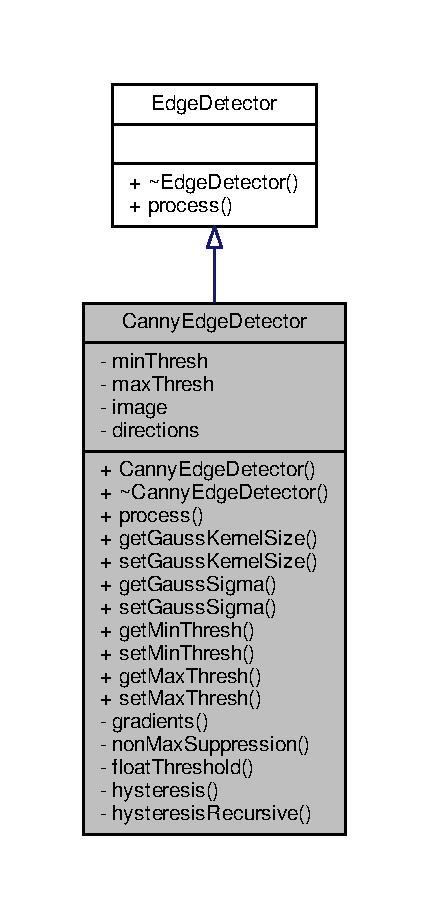
\includegraphics[width=206pt]{d3/d83/class_canny_edge_detector__inherit__graph}
\end{center}
\end{figure}


Граф связей класса Canny\+Edge\+Detector\+:
\nopagebreak
\begin{figure}[H]
\begin{center}
\leavevmode
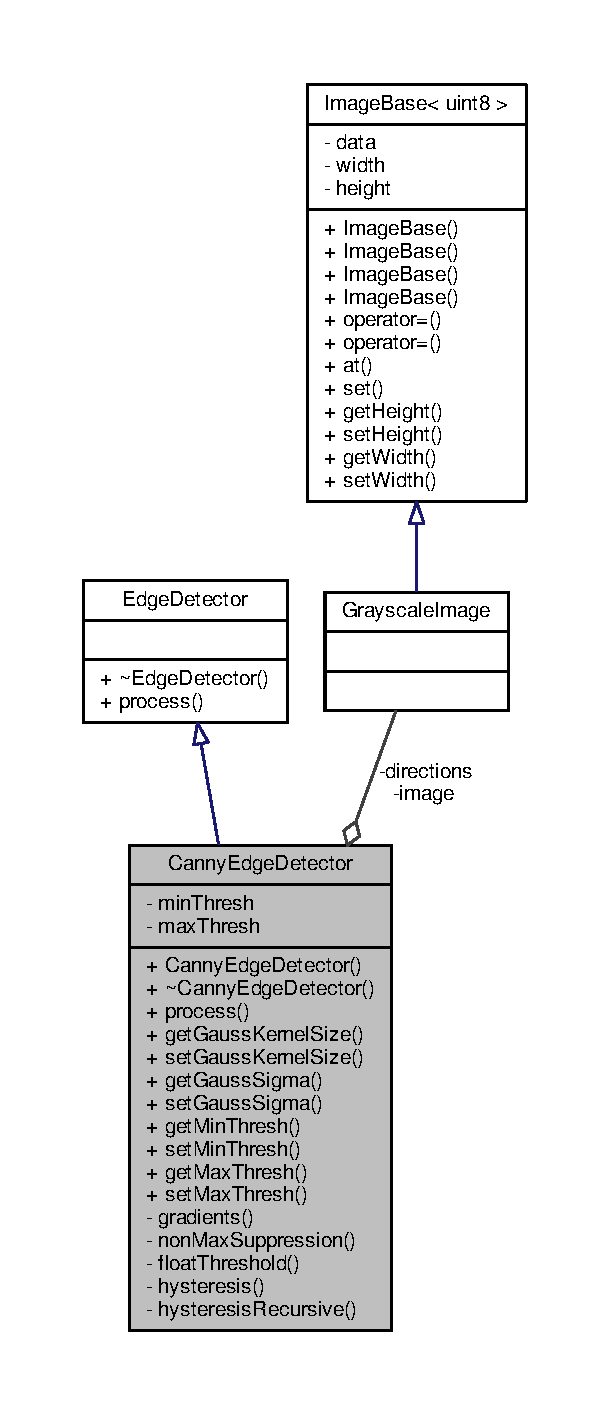
\includegraphics[height=550pt]{d0/dd8/class_canny_edge_detector__coll__graph}
\end{center}
\end{figure}
\subsection*{Открытые члены}
\begin{DoxyCompactItemize}
\item 
\hyperlink{class_canny_edge_detector_a6f7de6f12f8b52563d28e612a46f7a0d}{Canny\+Edge\+Detector} (\hyperlink{number_8h_a43d43196463bde49cb067f5c20ab8481}{int32} \hyperlink{class_canny_edge_detector_ae88472e936f883044b00e8cd50f662c6}{min\+Thresh}=80, \hyperlink{number_8h_a43d43196463bde49cb067f5c20ab8481}{int32} \hyperlink{class_canny_edge_detector_ab551b06077d0221f1caa6e5e4cce48d9}{max\+Thresh}=100)
\item 
virtual \hyperlink{class_canny_edge_detector_ad6f031b85ac2fc2f916ecaa04c536c01}{$\sim$\+Canny\+Edge\+Detector} ()
\item 
virtual void \hyperlink{class_canny_edge_detector_ae97e095e14e43d763a8fc2563f6e9a87}{process} (\hyperlink{class_image}{Image} \&\hyperlink{class_canny_edge_detector_a271e3c9036a5cb2611bb1b7da4d7d146}{image})
\item 
\hyperlink{number_8h_a43d43196463bde49cb067f5c20ab8481}{int32} \hyperlink{class_canny_edge_detector_a38218d65e7d450dc226e3bbb0c7043e9}{get\+Gauss\+Kernel\+Size} () const 
\item 
void \hyperlink{class_canny_edge_detector_adb6b71e26f03edea19d3fef041fd6cbd}{set\+Gauss\+Kernel\+Size} (\hyperlink{number_8h_a43d43196463bde49cb067f5c20ab8481}{int32} value)
\item 
float \hyperlink{class_canny_edge_detector_ac3e362832dcd3e18801bed15856e79b4}{get\+Gauss\+Sigma} () const 
\item 
void \hyperlink{class_canny_edge_detector_afc77ac77d033264009ea66670eeec9d0}{set\+Gauss\+Sigma} (float value)
\item 
\hyperlink{number_8h_a43d43196463bde49cb067f5c20ab8481}{int32} \hyperlink{class_canny_edge_detector_aa0ae63194968f376d4ea6e6d7e13f285}{get\+Min\+Thresh} () const 
\item 
void \hyperlink{class_canny_edge_detector_a825df00f677a9a949d0dcb87939a99b5}{set\+Min\+Thresh} (\hyperlink{number_8h_a43d43196463bde49cb067f5c20ab8481}{int32} value)
\item 
\hyperlink{number_8h_a43d43196463bde49cb067f5c20ab8481}{int32} \hyperlink{class_canny_edge_detector_aa3cb693f65b9a07e5f245d7ecadf9c5c}{get\+Max\+Thresh} () const 
\item 
void \hyperlink{class_canny_edge_detector_ae48e5be375a3a3d23c4dc81a158149c7}{set\+Max\+Thresh} (\hyperlink{number_8h_a43d43196463bde49cb067f5c20ab8481}{int32} value)
\end{DoxyCompactItemize}
\subsection*{Закрытые члены}
\begin{DoxyCompactItemize}
\item 
void \hyperlink{class_canny_edge_detector_ad5843016a5e861eed74fa24f4abd688b}{gradients} ()
\item 
void \hyperlink{class_canny_edge_detector_a8622531b7410c002284f466df043af13}{non\+Max\+Suppression} ()
\item 
void \hyperlink{class_canny_edge_detector_a0c6b710be023dec7cfd38e55d42066a3}{float\+Threshold} ()
\item 
void \hyperlink{class_canny_edge_detector_ab4bf8eb092943ab7042762ee48aeb0c1}{hysteresis} ()
\item 
void \hyperlink{class_canny_edge_detector_a3f180b6eb26a8afa34a03c8cdd0781ca}{hysteresis\+Recursive} (\hyperlink{number_8h_a1134b580f8da4de94ca6b1de4d37975e}{uint32} y, \hyperlink{number_8h_a1134b580f8da4de94ca6b1de4d37975e}{uint32} x)
\end{DoxyCompactItemize}
\subsection*{Закрытые данные}
\begin{DoxyCompactItemize}
\item 
\hyperlink{number_8h_a43d43196463bde49cb067f5c20ab8481}{int32} \hyperlink{class_canny_edge_detector_ae88472e936f883044b00e8cd50f662c6}{min\+Thresh}
\item 
\hyperlink{number_8h_a43d43196463bde49cb067f5c20ab8481}{int32} \hyperlink{class_canny_edge_detector_ab551b06077d0221f1caa6e5e4cce48d9}{max\+Thresh}
\item 
\hyperlink{class_grayscale_image}{Grayscale\+Image} \hyperlink{class_canny_edge_detector_a271e3c9036a5cb2611bb1b7da4d7d146}{image}
\item 
\hyperlink{class_grayscale_image}{Grayscale\+Image} \hyperlink{class_canny_edge_detector_a96275be60c2ffdc3798384f7a3588684}{directions}
\end{DoxyCompactItemize}


\subsection{Подробное описание}


См. определение в файле cannyedgedetector.\+h строка 8



\subsection{Конструктор(ы)}
\index{Canny\+Edge\+Detector@{Canny\+Edge\+Detector}!Canny\+Edge\+Detector@{Canny\+Edge\+Detector}}
\index{Canny\+Edge\+Detector@{Canny\+Edge\+Detector}!Canny\+Edge\+Detector@{Canny\+Edge\+Detector}}
\subsubsection[{\texorpdfstring{Canny\+Edge\+Detector(int32 min\+Thresh=80, int32 max\+Thresh=100)}{CannyEdgeDetector(int32 minThresh=80, int32 maxThresh=100)}}]{\setlength{\rightskip}{0pt plus 5cm}Canny\+Edge\+Detector\+::\+Canny\+Edge\+Detector (
\begin{DoxyParamCaption}
\item[{{\bf int32}}]{min\+Thresh = {\ttfamily 80}, }
\item[{{\bf int32}}]{max\+Thresh = {\ttfamily 100}}
\end{DoxyParamCaption}
)}\hypertarget{class_canny_edge_detector_a6f7de6f12f8b52563d28e612a46f7a0d}{}\label{class_canny_edge_detector_a6f7de6f12f8b52563d28e612a46f7a0d}


См. определение в файле cannyedgedetector.\+cpp строка 6

\index{Canny\+Edge\+Detector@{Canny\+Edge\+Detector}!````~Canny\+Edge\+Detector@{$\sim$\+Canny\+Edge\+Detector}}
\index{````~Canny\+Edge\+Detector@{$\sim$\+Canny\+Edge\+Detector}!Canny\+Edge\+Detector@{Canny\+Edge\+Detector}}
\subsubsection[{\texorpdfstring{$\sim$\+Canny\+Edge\+Detector()}{~CannyEdgeDetector()}}]{\setlength{\rightskip}{0pt plus 5cm}Canny\+Edge\+Detector\+::$\sim$\+Canny\+Edge\+Detector (
\begin{DoxyParamCaption}
{}
\end{DoxyParamCaption}
)\hspace{0.3cm}{\ttfamily [virtual]}}\hypertarget{class_canny_edge_detector_ad6f031b85ac2fc2f916ecaa04c536c01}{}\label{class_canny_edge_detector_ad6f031b85ac2fc2f916ecaa04c536c01}


См. определение в файле cannyedgedetector.\+cpp строка 12



\subsection{Методы}
\index{Canny\+Edge\+Detector@{Canny\+Edge\+Detector}!float\+Threshold@{float\+Threshold}}
\index{float\+Threshold@{float\+Threshold}!Canny\+Edge\+Detector@{Canny\+Edge\+Detector}}
\subsubsection[{\texorpdfstring{float\+Threshold()}{floatThreshold()}}]{\setlength{\rightskip}{0pt plus 5cm}void Canny\+Edge\+Detector\+::float\+Threshold (
\begin{DoxyParamCaption}
{}
\end{DoxyParamCaption}
)\hspace{0.3cm}{\ttfamily [private]}}\hypertarget{class_canny_edge_detector_a0c6b710be023dec7cfd38e55d42066a3}{}\label{class_canny_edge_detector_a0c6b710be023dec7cfd38e55d42066a3}


См. определение в файле cannyedgedetector.\+cpp строка 143

\index{Canny\+Edge\+Detector@{Canny\+Edge\+Detector}!get\+Gauss\+Kernel\+Size@{get\+Gauss\+Kernel\+Size}}
\index{get\+Gauss\+Kernel\+Size@{get\+Gauss\+Kernel\+Size}!Canny\+Edge\+Detector@{Canny\+Edge\+Detector}}
\subsubsection[{\texorpdfstring{get\+Gauss\+Kernel\+Size() const }{getGaussKernelSize() const }}]{\setlength{\rightskip}{0pt plus 5cm}{\bf int32} Canny\+Edge\+Detector\+::get\+Gauss\+Kernel\+Size (
\begin{DoxyParamCaption}
{}
\end{DoxyParamCaption}
) const}\hypertarget{class_canny_edge_detector_a38218d65e7d450dc226e3bbb0c7043e9}{}\label{class_canny_edge_detector_a38218d65e7d450dc226e3bbb0c7043e9}
\index{Canny\+Edge\+Detector@{Canny\+Edge\+Detector}!get\+Gauss\+Sigma@{get\+Gauss\+Sigma}}
\index{get\+Gauss\+Sigma@{get\+Gauss\+Sigma}!Canny\+Edge\+Detector@{Canny\+Edge\+Detector}}
\subsubsection[{\texorpdfstring{get\+Gauss\+Sigma() const }{getGaussSigma() const }}]{\setlength{\rightskip}{0pt plus 5cm}float Canny\+Edge\+Detector\+::get\+Gauss\+Sigma (
\begin{DoxyParamCaption}
{}
\end{DoxyParamCaption}
) const}\hypertarget{class_canny_edge_detector_ac3e362832dcd3e18801bed15856e79b4}{}\label{class_canny_edge_detector_ac3e362832dcd3e18801bed15856e79b4}
\index{Canny\+Edge\+Detector@{Canny\+Edge\+Detector}!get\+Max\+Thresh@{get\+Max\+Thresh}}
\index{get\+Max\+Thresh@{get\+Max\+Thresh}!Canny\+Edge\+Detector@{Canny\+Edge\+Detector}}
\subsubsection[{\texorpdfstring{get\+Max\+Thresh() const }{getMaxThresh() const }}]{\setlength{\rightskip}{0pt plus 5cm}{\bf int32} Canny\+Edge\+Detector\+::get\+Max\+Thresh (
\begin{DoxyParamCaption}
{}
\end{DoxyParamCaption}
) const}\hypertarget{class_canny_edge_detector_aa3cb693f65b9a07e5f245d7ecadf9c5c}{}\label{class_canny_edge_detector_aa3cb693f65b9a07e5f245d7ecadf9c5c}


См. определение в файле cannyedgedetector.\+cpp строка 243

\index{Canny\+Edge\+Detector@{Canny\+Edge\+Detector}!get\+Min\+Thresh@{get\+Min\+Thresh}}
\index{get\+Min\+Thresh@{get\+Min\+Thresh}!Canny\+Edge\+Detector@{Canny\+Edge\+Detector}}
\subsubsection[{\texorpdfstring{get\+Min\+Thresh() const }{getMinThresh() const }}]{\setlength{\rightskip}{0pt plus 5cm}{\bf int32} Canny\+Edge\+Detector\+::get\+Min\+Thresh (
\begin{DoxyParamCaption}
{}
\end{DoxyParamCaption}
) const}\hypertarget{class_canny_edge_detector_aa0ae63194968f376d4ea6e6d7e13f285}{}\label{class_canny_edge_detector_aa0ae63194968f376d4ea6e6d7e13f285}


См. определение в файле cannyedgedetector.\+cpp строка 253

\index{Canny\+Edge\+Detector@{Canny\+Edge\+Detector}!gradients@{gradients}}
\index{gradients@{gradients}!Canny\+Edge\+Detector@{Canny\+Edge\+Detector}}
\subsubsection[{\texorpdfstring{gradients()}{gradients()}}]{\setlength{\rightskip}{0pt plus 5cm}void Canny\+Edge\+Detector\+::gradients (
\begin{DoxyParamCaption}
{}
\end{DoxyParamCaption}
)\hspace{0.3cm}{\ttfamily [private]}}\hypertarget{class_canny_edge_detector_ad5843016a5e861eed74fa24f4abd688b}{}\label{class_canny_edge_detector_ad5843016a5e861eed74fa24f4abd688b}


См. определение в файле cannyedgedetector.\+cpp строка 28

\index{Canny\+Edge\+Detector@{Canny\+Edge\+Detector}!hysteresis@{hysteresis}}
\index{hysteresis@{hysteresis}!Canny\+Edge\+Detector@{Canny\+Edge\+Detector}}
\subsubsection[{\texorpdfstring{hysteresis()}{hysteresis()}}]{\setlength{\rightskip}{0pt plus 5cm}void Canny\+Edge\+Detector\+::hysteresis (
\begin{DoxyParamCaption}
{}
\end{DoxyParamCaption}
)\hspace{0.3cm}{\ttfamily [private]}}\hypertarget{class_canny_edge_detector_ab4bf8eb092943ab7042762ee48aeb0c1}{}\label{class_canny_edge_detector_ab4bf8eb092943ab7042762ee48aeb0c1}


См. определение в файле cannyedgedetector.\+cpp строка 169

\index{Canny\+Edge\+Detector@{Canny\+Edge\+Detector}!hysteresis\+Recursive@{hysteresis\+Recursive}}
\index{hysteresis\+Recursive@{hysteresis\+Recursive}!Canny\+Edge\+Detector@{Canny\+Edge\+Detector}}
\subsubsection[{\texorpdfstring{hysteresis\+Recursive(uint32 y, uint32 x)}{hysteresisRecursive(uint32 y, uint32 x)}}]{\setlength{\rightskip}{0pt plus 5cm}void Canny\+Edge\+Detector\+::hysteresis\+Recursive (
\begin{DoxyParamCaption}
\item[{{\bf uint32}}]{y, }
\item[{{\bf uint32}}]{x}
\end{DoxyParamCaption}
)\hspace{0.3cm}{\ttfamily [private]}}\hypertarget{class_canny_edge_detector_a3f180b6eb26a8afa34a03c8cdd0781ca}{}\label{class_canny_edge_detector_a3f180b6eb26a8afa34a03c8cdd0781ca}


См. определение в файле cannyedgedetector.\+cpp строка 194

\index{Canny\+Edge\+Detector@{Canny\+Edge\+Detector}!non\+Max\+Suppression@{non\+Max\+Suppression}}
\index{non\+Max\+Suppression@{non\+Max\+Suppression}!Canny\+Edge\+Detector@{Canny\+Edge\+Detector}}
\subsubsection[{\texorpdfstring{non\+Max\+Suppression()}{nonMaxSuppression()}}]{\setlength{\rightskip}{0pt plus 5cm}void Canny\+Edge\+Detector\+::non\+Max\+Suppression (
\begin{DoxyParamCaption}
{}
\end{DoxyParamCaption}
)\hspace{0.3cm}{\ttfamily [private]}}\hypertarget{class_canny_edge_detector_a8622531b7410c002284f466df043af13}{}\label{class_canny_edge_detector_a8622531b7410c002284f466df043af13}


См. определение в файле cannyedgedetector.\+cpp строка 102

\index{Canny\+Edge\+Detector@{Canny\+Edge\+Detector}!process@{process}}
\index{process@{process}!Canny\+Edge\+Detector@{Canny\+Edge\+Detector}}
\subsubsection[{\texorpdfstring{process(\+Image \&image)}{process(Image &image)}}]{\setlength{\rightskip}{0pt plus 5cm}void Canny\+Edge\+Detector\+::process (
\begin{DoxyParamCaption}
\item[{{\bf Image} \&}]{image}
\end{DoxyParamCaption}
)\hspace{0.3cm}{\ttfamily [virtual]}}\hypertarget{class_canny_edge_detector_ae97e095e14e43d763a8fc2563f6e9a87}{}\label{class_canny_edge_detector_ae97e095e14e43d763a8fc2563f6e9a87}


Замещает \hyperlink{class_edge_detector_aefa2d90e960e7dc3171bccadbed4a13e}{Edge\+Detector}.



См. определение в файле cannyedgedetector.\+cpp строка 16

\index{Canny\+Edge\+Detector@{Canny\+Edge\+Detector}!set\+Gauss\+Kernel\+Size@{set\+Gauss\+Kernel\+Size}}
\index{set\+Gauss\+Kernel\+Size@{set\+Gauss\+Kernel\+Size}!Canny\+Edge\+Detector@{Canny\+Edge\+Detector}}
\subsubsection[{\texorpdfstring{set\+Gauss\+Kernel\+Size(int32 value)}{setGaussKernelSize(int32 value)}}]{\setlength{\rightskip}{0pt plus 5cm}void Canny\+Edge\+Detector\+::set\+Gauss\+Kernel\+Size (
\begin{DoxyParamCaption}
\item[{{\bf int32}}]{value}
\end{DoxyParamCaption}
)}\hypertarget{class_canny_edge_detector_adb6b71e26f03edea19d3fef041fd6cbd}{}\label{class_canny_edge_detector_adb6b71e26f03edea19d3fef041fd6cbd}
\index{Canny\+Edge\+Detector@{Canny\+Edge\+Detector}!set\+Gauss\+Sigma@{set\+Gauss\+Sigma}}
\index{set\+Gauss\+Sigma@{set\+Gauss\+Sigma}!Canny\+Edge\+Detector@{Canny\+Edge\+Detector}}
\subsubsection[{\texorpdfstring{set\+Gauss\+Sigma(float value)}{setGaussSigma(float value)}}]{\setlength{\rightskip}{0pt plus 5cm}void Canny\+Edge\+Detector\+::set\+Gauss\+Sigma (
\begin{DoxyParamCaption}
\item[{float}]{value}
\end{DoxyParamCaption}
)}\hypertarget{class_canny_edge_detector_afc77ac77d033264009ea66670eeec9d0}{}\label{class_canny_edge_detector_afc77ac77d033264009ea66670eeec9d0}
\index{Canny\+Edge\+Detector@{Canny\+Edge\+Detector}!set\+Max\+Thresh@{set\+Max\+Thresh}}
\index{set\+Max\+Thresh@{set\+Max\+Thresh}!Canny\+Edge\+Detector@{Canny\+Edge\+Detector}}
\subsubsection[{\texorpdfstring{set\+Max\+Thresh(int32 value)}{setMaxThresh(int32 value)}}]{\setlength{\rightskip}{0pt plus 5cm}void Canny\+Edge\+Detector\+::set\+Max\+Thresh (
\begin{DoxyParamCaption}
\item[{{\bf int32}}]{value}
\end{DoxyParamCaption}
)}\hypertarget{class_canny_edge_detector_ae48e5be375a3a3d23c4dc81a158149c7}{}\label{class_canny_edge_detector_ae48e5be375a3a3d23c4dc81a158149c7}


См. определение в файле cannyedgedetector.\+cpp строка 248

\index{Canny\+Edge\+Detector@{Canny\+Edge\+Detector}!set\+Min\+Thresh@{set\+Min\+Thresh}}
\index{set\+Min\+Thresh@{set\+Min\+Thresh}!Canny\+Edge\+Detector@{Canny\+Edge\+Detector}}
\subsubsection[{\texorpdfstring{set\+Min\+Thresh(int32 value)}{setMinThresh(int32 value)}}]{\setlength{\rightskip}{0pt plus 5cm}void Canny\+Edge\+Detector\+::set\+Min\+Thresh (
\begin{DoxyParamCaption}
\item[{{\bf int32}}]{value}
\end{DoxyParamCaption}
)}\hypertarget{class_canny_edge_detector_a825df00f677a9a949d0dcb87939a99b5}{}\label{class_canny_edge_detector_a825df00f677a9a949d0dcb87939a99b5}


См. определение в файле cannyedgedetector.\+cpp строка 258



\subsection{Данные класса}
\index{Canny\+Edge\+Detector@{Canny\+Edge\+Detector}!directions@{directions}}
\index{directions@{directions}!Canny\+Edge\+Detector@{Canny\+Edge\+Detector}}
\subsubsection[{\texorpdfstring{directions}{directions}}]{\setlength{\rightskip}{0pt plus 5cm}{\bf Grayscale\+Image} Canny\+Edge\+Detector\+::directions\hspace{0.3cm}{\ttfamily [private]}}\hypertarget{class_canny_edge_detector_a96275be60c2ffdc3798384f7a3588684}{}\label{class_canny_edge_detector_a96275be60c2ffdc3798384f7a3588684}


См. определение в файле cannyedgedetector.\+h строка 39

\index{Canny\+Edge\+Detector@{Canny\+Edge\+Detector}!image@{image}}
\index{image@{image}!Canny\+Edge\+Detector@{Canny\+Edge\+Detector}}
\subsubsection[{\texorpdfstring{image}{image}}]{\setlength{\rightskip}{0pt plus 5cm}{\bf Grayscale\+Image} Canny\+Edge\+Detector\+::image\hspace{0.3cm}{\ttfamily [private]}}\hypertarget{class_canny_edge_detector_a271e3c9036a5cb2611bb1b7da4d7d146}{}\label{class_canny_edge_detector_a271e3c9036a5cb2611bb1b7da4d7d146}


См. определение в файле cannyedgedetector.\+h строка 38

\index{Canny\+Edge\+Detector@{Canny\+Edge\+Detector}!max\+Thresh@{max\+Thresh}}
\index{max\+Thresh@{max\+Thresh}!Canny\+Edge\+Detector@{Canny\+Edge\+Detector}}
\subsubsection[{\texorpdfstring{max\+Thresh}{maxThresh}}]{\setlength{\rightskip}{0pt plus 5cm}{\bf int32} Canny\+Edge\+Detector\+::max\+Thresh\hspace{0.3cm}{\ttfamily [private]}}\hypertarget{class_canny_edge_detector_ab551b06077d0221f1caa6e5e4cce48d9}{}\label{class_canny_edge_detector_ab551b06077d0221f1caa6e5e4cce48d9}


См. определение в файле cannyedgedetector.\+h строка 36

\index{Canny\+Edge\+Detector@{Canny\+Edge\+Detector}!min\+Thresh@{min\+Thresh}}
\index{min\+Thresh@{min\+Thresh}!Canny\+Edge\+Detector@{Canny\+Edge\+Detector}}
\subsubsection[{\texorpdfstring{min\+Thresh}{minThresh}}]{\setlength{\rightskip}{0pt plus 5cm}{\bf int32} Canny\+Edge\+Detector\+::min\+Thresh\hspace{0.3cm}{\ttfamily [private]}}\hypertarget{class_canny_edge_detector_ae88472e936f883044b00e8cd50f662c6}{}\label{class_canny_edge_detector_ae88472e936f883044b00e8cd50f662c6}


См. определение в файле cannyedgedetector.\+h строка 35



Объявления и описания членов классов находятся в файлах\+:\begin{DoxyCompactItemize}
\item 
Projects/labs/course\+\_\+project\+\_\+cg/src/algorithm/edgedetector/\hyperlink{cannyedgedetector_8h}{cannyedgedetector.\+h}\item 
Projects/labs/course\+\_\+project\+\_\+cg/src/algorithm/edgedetector/\hyperlink{cannyedgedetector_8cpp}{cannyedgedetector.\+cpp}\end{DoxyCompactItemize}

\hypertarget{class_color}{}\section{Класс Color}
\label{class_color}\index{Color@{Color}}


{\ttfamily \#include $<$color.\+h$>$}



Граф связей класса Color\+:
\nopagebreak
\begin{figure}[H]
\begin{center}
\leavevmode
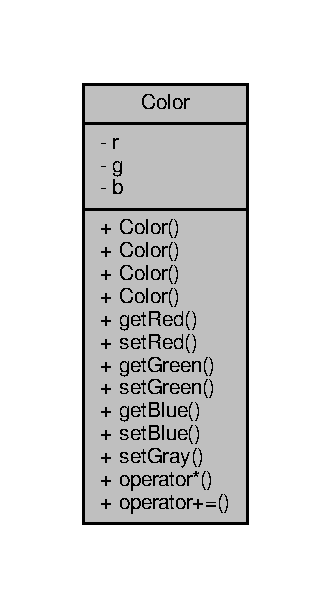
\includegraphics[width=159pt]{d2/d71/class_color__coll__graph}
\end{center}
\end{figure}
\subsection*{Открытые члены}
\begin{DoxyCompactItemize}
\item 
\hyperlink{class_color_a9a742cbe9f9f4037f5d9f4e81a9b2428}{Color} ()
\item 
\hyperlink{class_color_a9e2a61644848b70eff8103fe538e1b30}{Color} (\hyperlink{number_8h_adde6aaee8457bee49c2a92621fe22b79}{uint8} \hyperlink{class_color_ac25ae2b764ad9bbf8b8c79141f84d4ae}{r}, \hyperlink{number_8h_adde6aaee8457bee49c2a92621fe22b79}{uint8} \hyperlink{class_color_a895f2e61ca018a91877f52021f8748bd}{g}, \hyperlink{number_8h_adde6aaee8457bee49c2a92621fe22b79}{uint8} \hyperlink{class_color_a177ce5853f9bb12fda1c545dfb6f4ddf}{b})
\item 
\hyperlink{class_color_a7b075d27e3bbdde7cbe648dc3b804261}{Color} (const \hyperlink{class_color}{Color} \&color)
\item 
\hyperlink{class_color_a03aa495dec904466b0986feaa884bb8b}{Color} (\hyperlink{number_8h_adde6aaee8457bee49c2a92621fe22b79}{uint8} gray)
\item 
\hyperlink{number_8h_adde6aaee8457bee49c2a92621fe22b79}{uint8} \hyperlink{class_color_aaf34b98c81cfe8ec2682cc38761a4d5c}{get\+Red} () const 
\item 
void \hyperlink{class_color_a0db91f928764aa5fef82e92f55e34a2f}{set\+Red} (\hyperlink{number_8h_adde6aaee8457bee49c2a92621fe22b79}{uint8} value)
\item 
\hyperlink{number_8h_adde6aaee8457bee49c2a92621fe22b79}{uint8} \hyperlink{class_color_affb4bc39163b1c057e338125ed377494}{get\+Green} () const 
\item 
void \hyperlink{class_color_a35f06f6d8e5b2e57366ce2b3911b8d34}{set\+Green} (\hyperlink{number_8h_adde6aaee8457bee49c2a92621fe22b79}{uint8} value)
\item 
\hyperlink{number_8h_adde6aaee8457bee49c2a92621fe22b79}{uint8} \hyperlink{class_color_ad3adb9f5cc739957f9dbf053d2641de2}{get\+Blue} () const 
\item 
void \hyperlink{class_color_a957be1669566c9422dc48595d21547a1}{set\+Blue} (\hyperlink{number_8h_adde6aaee8457bee49c2a92621fe22b79}{uint8} value)
\item 
void \hyperlink{class_color_a0524f53d56d0e27be194f3c02644c6da}{set\+Gray} (\hyperlink{number_8h_adde6aaee8457bee49c2a92621fe22b79}{uint8} gray)
\item 
\hyperlink{class_color}{Color} \hyperlink{class_color_ab9427899af3ac7ef621c81a49633d1cb}{operator$\ast$} (float factor) const 
\item 
\hyperlink{class_color}{Color} \& \hyperlink{class_color_a26fc45655619e26ab7606823e39d80eb}{operator+=} (const \hyperlink{class_color}{Color} \&other)
\end{DoxyCompactItemize}
\subsection*{Закрытые данные}
\begin{DoxyCompactItemize}
\item 
\hyperlink{number_8h_adde6aaee8457bee49c2a92621fe22b79}{uint8} \hyperlink{class_color_ac25ae2b764ad9bbf8b8c79141f84d4ae}{r}
\item 
\hyperlink{number_8h_adde6aaee8457bee49c2a92621fe22b79}{uint8} \hyperlink{class_color_a895f2e61ca018a91877f52021f8748bd}{g}
\item 
\hyperlink{number_8h_adde6aaee8457bee49c2a92621fe22b79}{uint8} \hyperlink{class_color_a177ce5853f9bb12fda1c545dfb6f4ddf}{b}
\end{DoxyCompactItemize}


\subsection{Подробное описание}


См. определение в файле color.\+h строка 6



\subsection{Конструктор(ы)}
\index{Color@{Color}!Color@{Color}}
\index{Color@{Color}!Color@{Color}}
\subsubsection[{\texorpdfstring{Color()}{Color()}}]{\setlength{\rightskip}{0pt plus 5cm}Color\+::\+Color (
\begin{DoxyParamCaption}
{}
\end{DoxyParamCaption}
)}\hypertarget{class_color_a9a742cbe9f9f4037f5d9f4e81a9b2428}{}\label{class_color_a9a742cbe9f9f4037f5d9f4e81a9b2428}


См. определение в файле color.\+cpp строка 5

\index{Color@{Color}!Color@{Color}}
\index{Color@{Color}!Color@{Color}}
\subsubsection[{\texorpdfstring{Color(uint8 r, uint8 g, uint8 b)}{Color(uint8 r, uint8 g, uint8 b)}}]{\setlength{\rightskip}{0pt plus 5cm}Color\+::\+Color (
\begin{DoxyParamCaption}
\item[{{\bf uint8}}]{r, }
\item[{{\bf uint8}}]{g, }
\item[{{\bf uint8}}]{b}
\end{DoxyParamCaption}
)}\hypertarget{class_color_a9e2a61644848b70eff8103fe538e1b30}{}\label{class_color_a9e2a61644848b70eff8103fe538e1b30}


См. определение в файле color.\+cpp строка 26

\index{Color@{Color}!Color@{Color}}
\index{Color@{Color}!Color@{Color}}
\subsubsection[{\texorpdfstring{Color(const Color \&color)}{Color(const Color &color)}}]{\setlength{\rightskip}{0pt plus 5cm}Color\+::\+Color (
\begin{DoxyParamCaption}
\item[{const {\bf Color} \&}]{color}
\end{DoxyParamCaption}
)}\hypertarget{class_color_a7b075d27e3bbdde7cbe648dc3b804261}{}\label{class_color_a7b075d27e3bbdde7cbe648dc3b804261}


См. определение в файле color.\+cpp строка 12

\index{Color@{Color}!Color@{Color}}
\index{Color@{Color}!Color@{Color}}
\subsubsection[{\texorpdfstring{Color(uint8 gray)}{Color(uint8 gray)}}]{\setlength{\rightskip}{0pt plus 5cm}Color\+::\+Color (
\begin{DoxyParamCaption}
\item[{{\bf uint8}}]{gray}
\end{DoxyParamCaption}
)}\hypertarget{class_color_a03aa495dec904466b0986feaa884bb8b}{}\label{class_color_a03aa495dec904466b0986feaa884bb8b}


См. определение в файле color.\+cpp строка 19



\subsection{Методы}
\index{Color@{Color}!get\+Blue@{get\+Blue}}
\index{get\+Blue@{get\+Blue}!Color@{Color}}
\subsubsection[{\texorpdfstring{get\+Blue() const }{getBlue() const }}]{\setlength{\rightskip}{0pt plus 5cm}{\bf uint8} Color\+::get\+Blue (
\begin{DoxyParamCaption}
{}
\end{DoxyParamCaption}
) const}\hypertarget{class_color_ad3adb9f5cc739957f9dbf053d2641de2}{}\label{class_color_ad3adb9f5cc739957f9dbf053d2641de2}


См. определение в файле color.\+cpp строка 53

\index{Color@{Color}!get\+Green@{get\+Green}}
\index{get\+Green@{get\+Green}!Color@{Color}}
\subsubsection[{\texorpdfstring{get\+Green() const }{getGreen() const }}]{\setlength{\rightskip}{0pt plus 5cm}{\bf uint8} Color\+::get\+Green (
\begin{DoxyParamCaption}
{}
\end{DoxyParamCaption}
) const}\hypertarget{class_color_affb4bc39163b1c057e338125ed377494}{}\label{class_color_affb4bc39163b1c057e338125ed377494}


См. определение в файле color.\+cpp строка 43

\index{Color@{Color}!get\+Red@{get\+Red}}
\index{get\+Red@{get\+Red}!Color@{Color}}
\subsubsection[{\texorpdfstring{get\+Red() const }{getRed() const }}]{\setlength{\rightskip}{0pt plus 5cm}{\bf uint8} Color\+::get\+Red (
\begin{DoxyParamCaption}
{}
\end{DoxyParamCaption}
) const}\hypertarget{class_color_aaf34b98c81cfe8ec2682cc38761a4d5c}{}\label{class_color_aaf34b98c81cfe8ec2682cc38761a4d5c}


См. определение в файле color.\+cpp строка 33

\index{Color@{Color}!operator$\ast$@{operator$\ast$}}
\index{operator$\ast$@{operator$\ast$}!Color@{Color}}
\subsubsection[{\texorpdfstring{operator$\ast$(float factor) const }{operator*(float factor) const }}]{\setlength{\rightskip}{0pt plus 5cm}{\bf Color} Color\+::operator$\ast$ (
\begin{DoxyParamCaption}
\item[{float}]{factor}
\end{DoxyParamCaption}
) const}\hypertarget{class_color_ab9427899af3ac7ef621c81a49633d1cb}{}\label{class_color_ab9427899af3ac7ef621c81a49633d1cb}


См. определение в файле color.\+cpp строка 68

\index{Color@{Color}!operator+=@{operator+=}}
\index{operator+=@{operator+=}!Color@{Color}}
\subsubsection[{\texorpdfstring{operator+=(const Color \&other)}{operator+=(const Color &other)}}]{\setlength{\rightskip}{0pt plus 5cm}{\bf Color} \& Color\+::operator+= (
\begin{DoxyParamCaption}
\item[{const {\bf Color} \&}]{other}
\end{DoxyParamCaption}
)}\hypertarget{class_color_a26fc45655619e26ab7606823e39d80eb}{}\label{class_color_a26fc45655619e26ab7606823e39d80eb}


См. определение в файле color.\+cpp строка 75

\index{Color@{Color}!set\+Blue@{set\+Blue}}
\index{set\+Blue@{set\+Blue}!Color@{Color}}
\subsubsection[{\texorpdfstring{set\+Blue(uint8 value)}{setBlue(uint8 value)}}]{\setlength{\rightskip}{0pt plus 5cm}void Color\+::set\+Blue (
\begin{DoxyParamCaption}
\item[{{\bf uint8}}]{value}
\end{DoxyParamCaption}
)}\hypertarget{class_color_a957be1669566c9422dc48595d21547a1}{}\label{class_color_a957be1669566c9422dc48595d21547a1}


См. определение в файле color.\+cpp строка 58

\index{Color@{Color}!set\+Gray@{set\+Gray}}
\index{set\+Gray@{set\+Gray}!Color@{Color}}
\subsubsection[{\texorpdfstring{set\+Gray(uint8 gray)}{setGray(uint8 gray)}}]{\setlength{\rightskip}{0pt plus 5cm}void Color\+::set\+Gray (
\begin{DoxyParamCaption}
\item[{{\bf uint8}}]{gray}
\end{DoxyParamCaption}
)}\hypertarget{class_color_a0524f53d56d0e27be194f3c02644c6da}{}\label{class_color_a0524f53d56d0e27be194f3c02644c6da}


См. определение в файле color.\+cpp строка 63

\index{Color@{Color}!set\+Green@{set\+Green}}
\index{set\+Green@{set\+Green}!Color@{Color}}
\subsubsection[{\texorpdfstring{set\+Green(uint8 value)}{setGreen(uint8 value)}}]{\setlength{\rightskip}{0pt plus 5cm}void Color\+::set\+Green (
\begin{DoxyParamCaption}
\item[{{\bf uint8}}]{value}
\end{DoxyParamCaption}
)}\hypertarget{class_color_a35f06f6d8e5b2e57366ce2b3911b8d34}{}\label{class_color_a35f06f6d8e5b2e57366ce2b3911b8d34}


См. определение в файле color.\+cpp строка 48

\index{Color@{Color}!set\+Red@{set\+Red}}
\index{set\+Red@{set\+Red}!Color@{Color}}
\subsubsection[{\texorpdfstring{set\+Red(uint8 value)}{setRed(uint8 value)}}]{\setlength{\rightskip}{0pt plus 5cm}void Color\+::set\+Red (
\begin{DoxyParamCaption}
\item[{{\bf uint8}}]{value}
\end{DoxyParamCaption}
)}\hypertarget{class_color_a0db91f928764aa5fef82e92f55e34a2f}{}\label{class_color_a0db91f928764aa5fef82e92f55e34a2f}


См. определение в файле color.\+cpp строка 38



\subsection{Данные класса}
\index{Color@{Color}!b@{b}}
\index{b@{b}!Color@{Color}}
\subsubsection[{\texorpdfstring{b}{b}}]{\setlength{\rightskip}{0pt plus 5cm}{\bf uint8} Color\+::b\hspace{0.3cm}{\ttfamily [private]}}\hypertarget{class_color_a177ce5853f9bb12fda1c545dfb6f4ddf}{}\label{class_color_a177ce5853f9bb12fda1c545dfb6f4ddf}


См. определение в файле color.\+h строка 29

\index{Color@{Color}!g@{g}}
\index{g@{g}!Color@{Color}}
\subsubsection[{\texorpdfstring{g}{g}}]{\setlength{\rightskip}{0pt plus 5cm}{\bf uint8} Color\+::g\hspace{0.3cm}{\ttfamily [private]}}\hypertarget{class_color_a895f2e61ca018a91877f52021f8748bd}{}\label{class_color_a895f2e61ca018a91877f52021f8748bd}


См. определение в файле color.\+h строка 29

\index{Color@{Color}!r@{r}}
\index{r@{r}!Color@{Color}}
\subsubsection[{\texorpdfstring{r}{r}}]{\setlength{\rightskip}{0pt plus 5cm}{\bf uint8} Color\+::r\hspace{0.3cm}{\ttfamily [private]}}\hypertarget{class_color_ac25ae2b764ad9bbf8b8c79141f84d4ae}{}\label{class_color_ac25ae2b764ad9bbf8b8c79141f84d4ae}


См. определение в файле color.\+h строка 29



Объявления и описания членов классов находятся в файлах\+:\begin{DoxyCompactItemize}
\item 
Projects/labs/course\+\_\+project\+\_\+cg/src/image/\hyperlink{color_8h}{color.\+h}\item 
Projects/labs/course\+\_\+project\+\_\+cg/src/image/\hyperlink{color_8cpp}{color.\+cpp}\end{DoxyCompactItemize}

\hypertarget{class_common_transformation}{}\section{Класс Common\+Transformation}
\label{class_common_transformation}\index{Common\+Transformation@{Common\+Transformation}}


{\ttfamily \#include $<$commontransformation.\+h$>$}



Граф наследования\+:Common\+Transformation\+:
\nopagebreak
\begin{figure}[H]
\begin{center}
\leavevmode
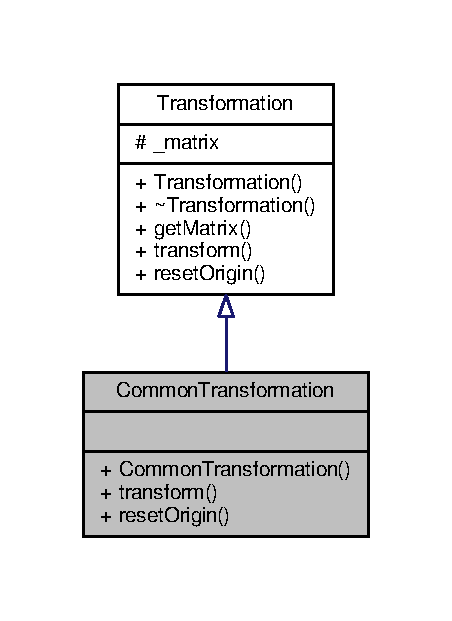
\includegraphics[width=217pt]{d0/d4d/class_common_transformation__inherit__graph}
\end{center}
\end{figure}


Граф связей класса Common\+Transformation\+:
\nopagebreak
\begin{figure}[H]
\begin{center}
\leavevmode
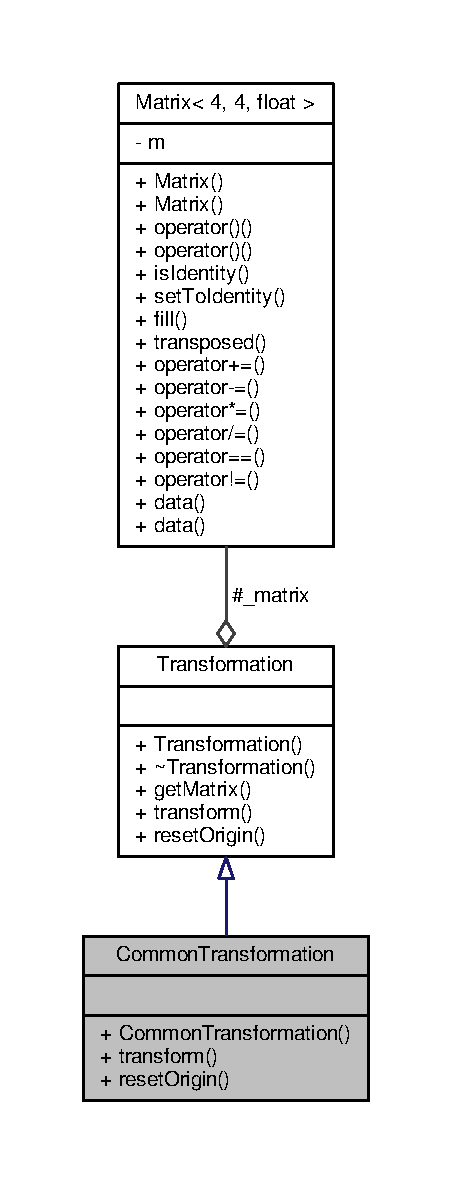
\includegraphics[height=550pt]{dc/d0d/class_common_transformation__coll__graph}
\end{center}
\end{figure}
\subsection*{Открытые члены}
\begin{DoxyCompactItemize}
\item 
\hyperlink{class_common_transformation_a6482f70fab18b0afa41bc9b2f1b56665}{Common\+Transformation} (const \hyperlink{matrix_8h_a077dce9756976f552e5703c34475d5e3}{Mat4} \&matrix)
\item 
virtual void \hyperlink{class_common_transformation_a7daef5b3ad4576a691b474d888c3dfd5}{transform} (\hyperlink{vec3_8h_a221ad8ea4d9be4111628ee1ca22ee3ba}{Vec3} \&vertex) const override
\item 
virtual void \hyperlink{class_common_transformation_a8f789aa59517fd1bf553e1846241eacc}{reset\+Origin} () override
\end{DoxyCompactItemize}
\subsection*{Дополнительные унаследованные члены}


\subsection{Подробное описание}


См. определение в файле commontransformation.\+h строка 7



\subsection{Конструктор(ы)}
\index{Common\+Transformation@{Common\+Transformation}!Common\+Transformation@{Common\+Transformation}}
\index{Common\+Transformation@{Common\+Transformation}!Common\+Transformation@{Common\+Transformation}}
\subsubsection[{\texorpdfstring{Common\+Transformation(const Mat4 \&matrix)}{CommonTransformation(const Mat4 &matrix)}}]{\setlength{\rightskip}{0pt plus 5cm}Common\+Transformation\+::\+Common\+Transformation (
\begin{DoxyParamCaption}
\item[{const {\bf Mat4} \&}]{matrix}
\end{DoxyParamCaption}
)}\hypertarget{class_common_transformation_a6482f70fab18b0afa41bc9b2f1b56665}{}\label{class_common_transformation_a6482f70fab18b0afa41bc9b2f1b56665}


См. определение в файле commontransformation.\+cpp строка 4



\subsection{Методы}
\index{Common\+Transformation@{Common\+Transformation}!reset\+Origin@{reset\+Origin}}
\index{reset\+Origin@{reset\+Origin}!Common\+Transformation@{Common\+Transformation}}
\subsubsection[{\texorpdfstring{reset\+Origin() override}{resetOrigin() override}}]{\setlength{\rightskip}{0pt plus 5cm}void Common\+Transformation\+::reset\+Origin (
\begin{DoxyParamCaption}
{}
\end{DoxyParamCaption}
)\hspace{0.3cm}{\ttfamily [override]}, {\ttfamily [virtual]}}\hypertarget{class_common_transformation_a8f789aa59517fd1bf553e1846241eacc}{}\label{class_common_transformation_a8f789aa59517fd1bf553e1846241eacc}


Замещает \hyperlink{class_transformation_a2bc354a92aeda699c7c12c54eb120038}{Transformation}.



См. определение в файле commontransformation.\+cpp строка 19

\index{Common\+Transformation@{Common\+Transformation}!transform@{transform}}
\index{transform@{transform}!Common\+Transformation@{Common\+Transformation}}
\subsubsection[{\texorpdfstring{transform(\+Vec3 \&vertex) const override}{transform(Vec3 &vertex) const override}}]{\setlength{\rightskip}{0pt plus 5cm}void Common\+Transformation\+::transform (
\begin{DoxyParamCaption}
\item[{{\bf Vec3} \&}]{vertex}
\end{DoxyParamCaption}
) const\hspace{0.3cm}{\ttfamily [override]}, {\ttfamily [virtual]}}\hypertarget{class_common_transformation_a7daef5b3ad4576a691b474d888c3dfd5}{}\label{class_common_transformation_a7daef5b3ad4576a691b474d888c3dfd5}


Замещает \hyperlink{class_transformation_a3800376d1f4a64ec6ba6abfa3e22c8ee}{Transformation}.



См. определение в файле commontransformation.\+cpp строка 9



Объявления и описания членов классов находятся в файлах\+:\begin{DoxyCompactItemize}
\item 
Projects/labs/course\+\_\+project\+\_\+cg/src/animation/\hyperlink{commontransformation_8h}{commontransformation.\+h}\item 
Projects/labs/course\+\_\+project\+\_\+cg/src/animation/\hyperlink{commontransformation_8cpp}{commontransformation.\+cpp}\end{DoxyCompactItemize}

\hypertarget{class_composite}{}\section{Класс Composite}
\label{class_composite}\index{Composite@{Composite}}


{\ttfamily \#include $<$composite.\+h$>$}



Граф наследования\+:Composite\+:
\nopagebreak
\begin{figure}[H]
\begin{center}
\leavevmode
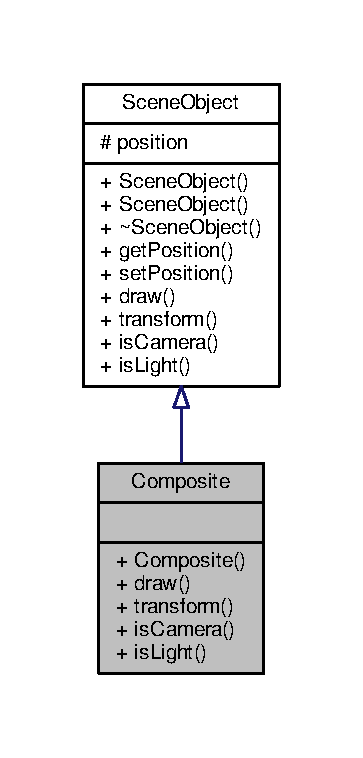
\includegraphics[width=174pt]{d5/d8c/class_composite__inherit__graph}
\end{center}
\end{figure}


Граф связей класса Composite\+:
\nopagebreak
\begin{figure}[H]
\begin{center}
\leavevmode
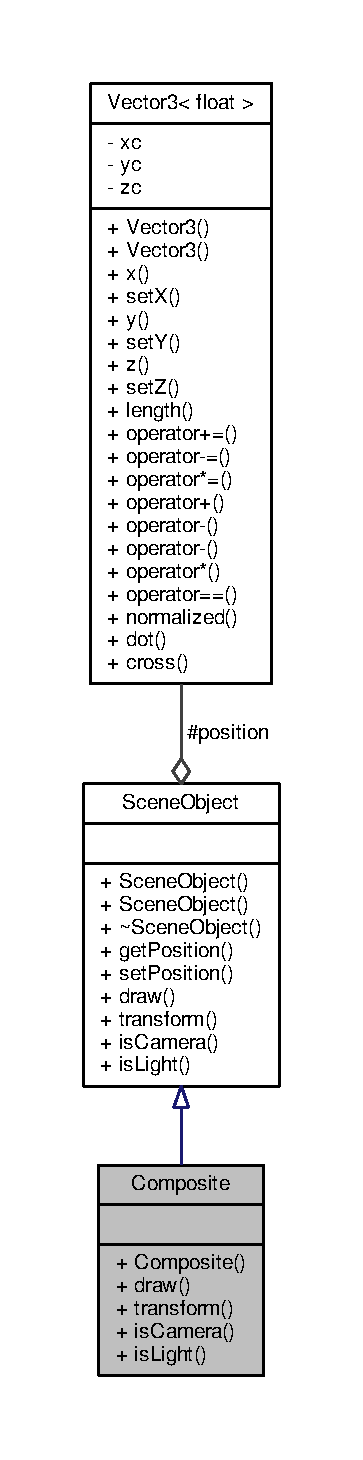
\includegraphics[height=550pt]{da/db3/class_composite__coll__graph}
\end{center}
\end{figure}
\subsection*{Открытые члены}
\begin{DoxyCompactItemize}
\item 
\hyperlink{class_composite_ad28832d957183a7f08dec72e6040db0a}{Composite} ()
\item 
virtual void \hyperlink{class_composite_a95e3d893a3e3ec8bbb2dc449278b64c4}{draw} (std\+::unique\+\_\+ptr$<$ \hyperlink{class_renderer}{Renderer} $>$ \&) override
\item 
virtual void \hyperlink{class_composite_afaae38bc8ef323cf05bf5710dafbeb39}{transform} (\hyperlink{class_transformation}{Transformation} \&) override
\item 
virtual bool \hyperlink{class_composite_a041e0a198c3c2fcc7b16f36a7511f7c3}{is\+Camera} () override
\item 
virtual bool \hyperlink{class_composite_a704e2e6583b8c553cbc5d1ddedea529d}{is\+Light} () override
\end{DoxyCompactItemize}
\subsection*{Дополнительные унаследованные члены}


\subsection{Подробное описание}


См. определение в файле composite.\+h строка 6



\subsection{Конструктор(ы)}
\index{Composite@{Composite}!Composite@{Composite}}
\index{Composite@{Composite}!Composite@{Composite}}
\subsubsection[{\texorpdfstring{Composite()}{Composite()}}]{\setlength{\rightskip}{0pt plus 5cm}Composite\+::\+Composite (
\begin{DoxyParamCaption}
{}
\end{DoxyParamCaption}
)}\hypertarget{class_composite_ad28832d957183a7f08dec72e6040db0a}{}\label{class_composite_ad28832d957183a7f08dec72e6040db0a}


См. определение в файле composite.\+cpp строка 3



\subsection{Методы}
\index{Composite@{Composite}!draw@{draw}}
\index{draw@{draw}!Composite@{Composite}}
\subsubsection[{\texorpdfstring{draw(std\+::unique\+\_\+ptr$<$ Renderer $>$ \&) override}{draw(std::unique_ptr< Renderer > &) override}}]{\setlength{\rightskip}{0pt plus 5cm}void Composite\+::draw (
\begin{DoxyParamCaption}
\item[{std\+::unique\+\_\+ptr$<$ {\bf Renderer} $>$ \&}]{}
\end{DoxyParamCaption}
)\hspace{0.3cm}{\ttfamily [override]}, {\ttfamily [virtual]}}\hypertarget{class_composite_a95e3d893a3e3ec8bbb2dc449278b64c4}{}\label{class_composite_a95e3d893a3e3ec8bbb2dc449278b64c4}


Замещает \hyperlink{class_scene_object_adc906ce4e4a896a351949ccabfd44016}{Scene\+Object}.



См. определение в файле composite.\+cpp строка 8

\index{Composite@{Composite}!is\+Camera@{is\+Camera}}
\index{is\+Camera@{is\+Camera}!Composite@{Composite}}
\subsubsection[{\texorpdfstring{is\+Camera() override}{isCamera() override}}]{\setlength{\rightskip}{0pt plus 5cm}bool Composite\+::is\+Camera (
\begin{DoxyParamCaption}
{}
\end{DoxyParamCaption}
)\hspace{0.3cm}{\ttfamily [override]}, {\ttfamily [virtual]}}\hypertarget{class_composite_a041e0a198c3c2fcc7b16f36a7511f7c3}{}\label{class_composite_a041e0a198c3c2fcc7b16f36a7511f7c3}


Замещает \hyperlink{class_scene_object_a6d7cb8b9a2c29f38fd039731e83167f4}{Scene\+Object}.



См. определение в файле composite.\+cpp строка 16

\index{Composite@{Composite}!is\+Light@{is\+Light}}
\index{is\+Light@{is\+Light}!Composite@{Composite}}
\subsubsection[{\texorpdfstring{is\+Light() override}{isLight() override}}]{\setlength{\rightskip}{0pt plus 5cm}bool Composite\+::is\+Light (
\begin{DoxyParamCaption}
{}
\end{DoxyParamCaption}
)\hspace{0.3cm}{\ttfamily [override]}, {\ttfamily [virtual]}}\hypertarget{class_composite_a704e2e6583b8c553cbc5d1ddedea529d}{}\label{class_composite_a704e2e6583b8c553cbc5d1ddedea529d}


Замещает \hyperlink{class_scene_object_a9c5b006b8a0e457634f15c19eb51ca73}{Scene\+Object}.



См. определение в файле composite.\+cpp строка 21

\index{Composite@{Composite}!transform@{transform}}
\index{transform@{transform}!Composite@{Composite}}
\subsubsection[{\texorpdfstring{transform(\+Transformation \&) override}{transform(Transformation &) override}}]{\setlength{\rightskip}{0pt plus 5cm}void Composite\+::transform (
\begin{DoxyParamCaption}
\item[{{\bf Transformation} \&}]{}
\end{DoxyParamCaption}
)\hspace{0.3cm}{\ttfamily [override]}, {\ttfamily [virtual]}}\hypertarget{class_composite_afaae38bc8ef323cf05bf5710dafbeb39}{}\label{class_composite_afaae38bc8ef323cf05bf5710dafbeb39}


Замещает \hyperlink{class_scene_object_a1b8a4b90f1200f1cd025d95964d43630}{Scene\+Object}.



См. определение в файле composite.\+cpp строка 12



Объявления и описания членов классов находятся в файлах\+:\begin{DoxyCompactItemize}
\item 
Projects/labs/course\+\_\+project\+\_\+cg/src/animation/\hyperlink{composite_8h}{composite.\+h}\item 
Projects/labs/course\+\_\+project\+\_\+cg/src/animation/\hyperlink{composite_8cpp}{composite.\+cpp}\end{DoxyCompactItemize}

\hypertarget{class_cylinder_size}{}\section{Класс Cylinder\+Size}
\label{class_cylinder_size}\index{Cylinder\+Size@{Cylinder\+Size}}


{\ttfamily \#include $<$cylindersize.\+h$>$}



Граф связей класса Cylinder\+Size\+:
\nopagebreak
\begin{figure}[H]
\begin{center}
\leavevmode
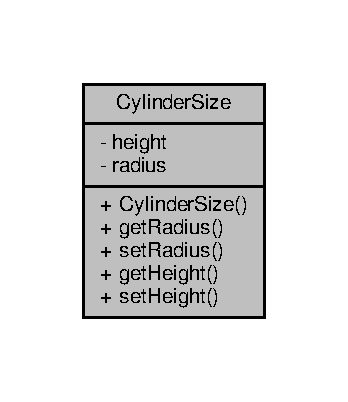
\includegraphics[width=167pt]{df/db6/class_cylinder_size__coll__graph}
\end{center}
\end{figure}
\subsection*{Открытые члены}
\begin{DoxyCompactItemize}
\item 
\hyperlink{class_cylinder_size_a9896a88f9cf7b392a72e79d913b7c241}{Cylinder\+Size} (float \hyperlink{class_cylinder_size_a64a31d3ecef008bc999f02797aa73ebf}{height}=0, float \hyperlink{class_cylinder_size_ac12aa459995c8467cf96d978b05e7ee5}{radius}=0)
\item 
float \hyperlink{class_cylinder_size_a69dbd81e8e5bda6a9efb6d0dd621dac4}{get\+Radius} () const 
\item 
void \hyperlink{class_cylinder_size_a7598cedd43027dfaea97ad273180ed63}{set\+Radius} (float value)
\item 
float \hyperlink{class_cylinder_size_aac6bbbc1e12cb65d0ca299eda89f43f0}{get\+Height} () const 
\item 
void \hyperlink{class_cylinder_size_afad35daeb0ed7d9c3b132a23de7412c0}{set\+Height} (float value)
\end{DoxyCompactItemize}
\subsection*{Закрытые данные}
\begin{DoxyCompactItemize}
\item 
float \hyperlink{class_cylinder_size_a64a31d3ecef008bc999f02797aa73ebf}{height}
\item 
float \hyperlink{class_cylinder_size_ac12aa459995c8467cf96d978b05e7ee5}{radius}
\end{DoxyCompactItemize}


\subsection{Подробное описание}


См. определение в файле cylindersize.\+h строка 5



\subsection{Конструктор(ы)}
\index{Cylinder\+Size@{Cylinder\+Size}!Cylinder\+Size@{Cylinder\+Size}}
\index{Cylinder\+Size@{Cylinder\+Size}!Cylinder\+Size@{Cylinder\+Size}}
\subsubsection[{\texorpdfstring{Cylinder\+Size(float height=0, float radius=0)}{CylinderSize(float height=0, float radius=0)}}]{\setlength{\rightskip}{0pt plus 5cm}Cylinder\+Size\+::\+Cylinder\+Size (
\begin{DoxyParamCaption}
\item[{float}]{height = {\ttfamily 0}, }
\item[{float}]{radius = {\ttfamily 0}}
\end{DoxyParamCaption}
)}\hypertarget{class_cylinder_size_a9896a88f9cf7b392a72e79d913b7c241}{}\label{class_cylinder_size_a9896a88f9cf7b392a72e79d913b7c241}


См. определение в файле cylindersize.\+cpp строка 3



\subsection{Методы}
\index{Cylinder\+Size@{Cylinder\+Size}!get\+Height@{get\+Height}}
\index{get\+Height@{get\+Height}!Cylinder\+Size@{Cylinder\+Size}}
\subsubsection[{\texorpdfstring{get\+Height() const }{getHeight() const }}]{\setlength{\rightskip}{0pt plus 5cm}float Cylinder\+Size\+::get\+Height (
\begin{DoxyParamCaption}
{}
\end{DoxyParamCaption}
) const}\hypertarget{class_cylinder_size_aac6bbbc1e12cb65d0ca299eda89f43f0}{}\label{class_cylinder_size_aac6bbbc1e12cb65d0ca299eda89f43f0}


См. определение в файле cylindersize.\+cpp строка 19

\index{Cylinder\+Size@{Cylinder\+Size}!get\+Radius@{get\+Radius}}
\index{get\+Radius@{get\+Radius}!Cylinder\+Size@{Cylinder\+Size}}
\subsubsection[{\texorpdfstring{get\+Radius() const }{getRadius() const }}]{\setlength{\rightskip}{0pt plus 5cm}float Cylinder\+Size\+::get\+Radius (
\begin{DoxyParamCaption}
{}
\end{DoxyParamCaption}
) const}\hypertarget{class_cylinder_size_a69dbd81e8e5bda6a9efb6d0dd621dac4}{}\label{class_cylinder_size_a69dbd81e8e5bda6a9efb6d0dd621dac4}


См. определение в файле cylindersize.\+cpp строка 9

\index{Cylinder\+Size@{Cylinder\+Size}!set\+Height@{set\+Height}}
\index{set\+Height@{set\+Height}!Cylinder\+Size@{Cylinder\+Size}}
\subsubsection[{\texorpdfstring{set\+Height(float value)}{setHeight(float value)}}]{\setlength{\rightskip}{0pt plus 5cm}void Cylinder\+Size\+::set\+Height (
\begin{DoxyParamCaption}
\item[{float}]{value}
\end{DoxyParamCaption}
)}\hypertarget{class_cylinder_size_afad35daeb0ed7d9c3b132a23de7412c0}{}\label{class_cylinder_size_afad35daeb0ed7d9c3b132a23de7412c0}


См. определение в файле cylindersize.\+cpp строка 24

\index{Cylinder\+Size@{Cylinder\+Size}!set\+Radius@{set\+Radius}}
\index{set\+Radius@{set\+Radius}!Cylinder\+Size@{Cylinder\+Size}}
\subsubsection[{\texorpdfstring{set\+Radius(float value)}{setRadius(float value)}}]{\setlength{\rightskip}{0pt plus 5cm}void Cylinder\+Size\+::set\+Radius (
\begin{DoxyParamCaption}
\item[{float}]{value}
\end{DoxyParamCaption}
)}\hypertarget{class_cylinder_size_a7598cedd43027dfaea97ad273180ed63}{}\label{class_cylinder_size_a7598cedd43027dfaea97ad273180ed63}


См. определение в файле cylindersize.\+cpp строка 14



\subsection{Данные класса}
\index{Cylinder\+Size@{Cylinder\+Size}!height@{height}}
\index{height@{height}!Cylinder\+Size@{Cylinder\+Size}}
\subsubsection[{\texorpdfstring{height}{height}}]{\setlength{\rightskip}{0pt plus 5cm}float Cylinder\+Size\+::height\hspace{0.3cm}{\ttfamily [private]}}\hypertarget{class_cylinder_size_a64a31d3ecef008bc999f02797aa73ebf}{}\label{class_cylinder_size_a64a31d3ecef008bc999f02797aa73ebf}


См. определение в файле cylindersize.\+h строка 17

\index{Cylinder\+Size@{Cylinder\+Size}!radius@{radius}}
\index{radius@{radius}!Cylinder\+Size@{Cylinder\+Size}}
\subsubsection[{\texorpdfstring{radius}{radius}}]{\setlength{\rightskip}{0pt plus 5cm}float Cylinder\+Size\+::radius\hspace{0.3cm}{\ttfamily [private]}}\hypertarget{class_cylinder_size_ac12aa459995c8467cf96d978b05e7ee5}{}\label{class_cylinder_size_ac12aa459995c8467cf96d978b05e7ee5}


См. определение в файле cylindersize.\+h строка 18



Объявления и описания членов классов находятся в файлах\+:\begin{DoxyCompactItemize}
\item 
Projects/labs/course\+\_\+project\+\_\+cg/src/math/\hyperlink{cylindersize_8h}{cylindersize.\+h}\item 
Projects/labs/course\+\_\+project\+\_\+cg/src/math/\hyperlink{cylindersize_8cpp}{cylindersize.\+cpp}\end{DoxyCompactItemize}

\hypertarget{class_cylinder_size_calculator}{}\section{Класс Cylinder\+Size\+Calculator}
\label{class_cylinder_size_calculator}\index{Cylinder\+Size\+Calculator@{Cylinder\+Size\+Calculator}}


{\ttfamily \#include $<$cylindersizecalculator.\+h$>$}



Граф наследования\+:Cylinder\+Size\+Calculator\+:
\nopagebreak
\begin{figure}[H]
\begin{center}
\leavevmode
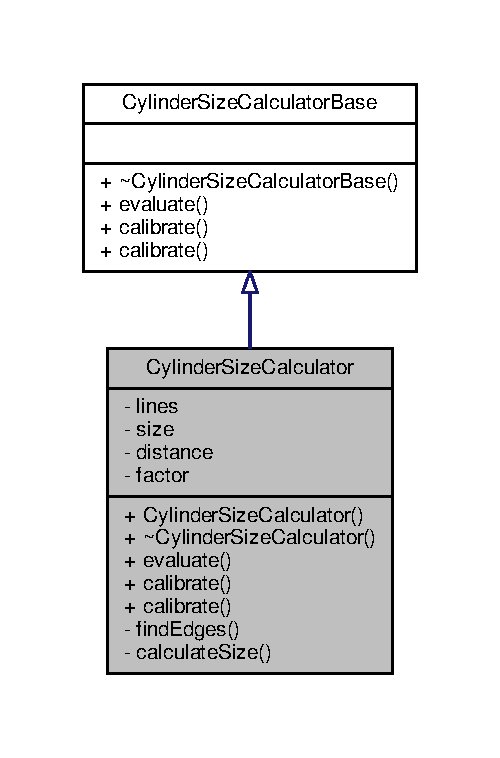
\includegraphics[width=240pt]{da/d4d/class_cylinder_size_calculator__inherit__graph}
\end{center}
\end{figure}


Граф связей класса Cylinder\+Size\+Calculator\+:
\nopagebreak
\begin{figure}[H]
\begin{center}
\leavevmode
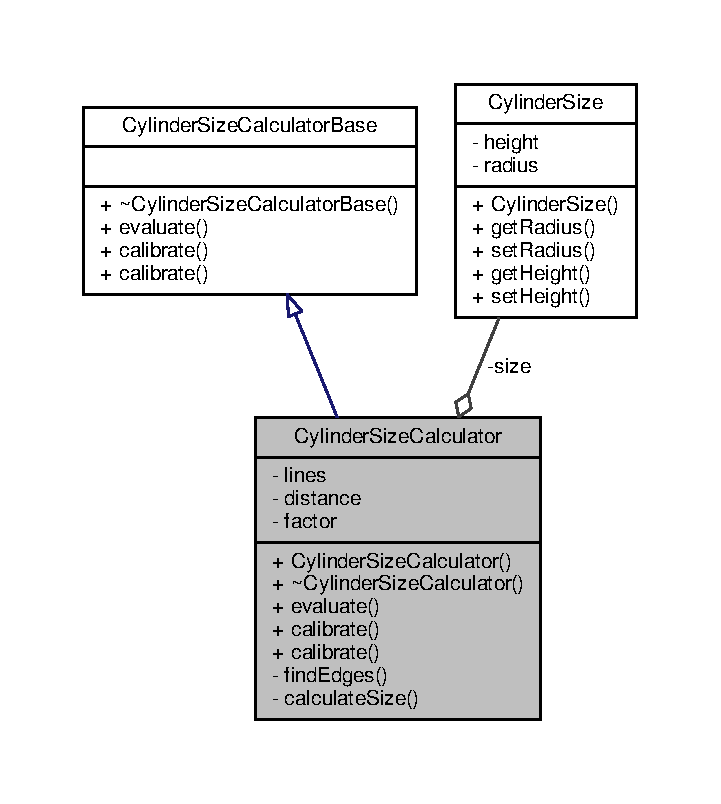
\includegraphics[width=346pt]{da/d2c/class_cylinder_size_calculator__coll__graph}
\end{center}
\end{figure}
\subsection*{Открытые члены}
\begin{DoxyCompactItemize}
\item 
\hyperlink{class_cylinder_size_calculator_ab4daaa75220e687cca3ce57e9db2fe57}{Cylinder\+Size\+Calculator} ()
\item 
virtual \hyperlink{class_cylinder_size_calculator_af8ff9a4ab970aa5fcdca273112789978}{$\sim$\+Cylinder\+Size\+Calculator} ()
\item 
virtual \hyperlink{class_cylinder_size}{Cylinder\+Size} \hyperlink{class_cylinder_size_calculator_a979a607bd694c5819355793d231c5df2}{evaluate} (const \hyperlink{class_cylinder_size_calculator_a7c30882e5312856d6757dc0022eb231f}{Lines} \&\hyperlink{class_cylinder_size_calculator_a8a329c2526e67545603769c720d76692}{lines})
\item 
virtual void \hyperlink{class_cylinder_size_calculator_a411f74a0f0baa7c393fe53c36d957fd4}{calibrate} (const std\+::vector$<$ \hyperlink{class_line}{Line} $>$ \&\hyperlink{class_cylinder_size_calculator_a8a329c2526e67545603769c720d76692}{lines}, float \hyperlink{class_cylinder_size_calculator_a1d88b87623a24582f968bb06acd80b8c}{distance}, float radius, float height)
\item 
virtual void \hyperlink{class_cylinder_size_calculator_ace80de293c2d4626b65e83fcb0fcde54}{calibrate} (float diag, float diag\+Px)
\end{DoxyCompactItemize}
\subsection*{Закрытые типы}
\begin{DoxyCompactItemize}
\item 
using \hyperlink{class_cylinder_size_calculator_a7c30882e5312856d6757dc0022eb231f}{Lines} = std\+::vector$<$ \hyperlink{class_line}{Line} $>$
\end{DoxyCompactItemize}
\subsection*{Закрытые члены}
\begin{DoxyCompactItemize}
\item 
void \hyperlink{class_cylinder_size_calculator_ad908e8325d6a03c7b4d1b55cf87eade9}{find\+Edges} ()
\item 
void \hyperlink{class_cylinder_size_calculator_a4afc5d76534bc67a394a0f78d21a4811}{calculate\+Size} ()
\end{DoxyCompactItemize}
\subsection*{Закрытые данные}
\begin{DoxyCompactItemize}
\item 
\hyperlink{class_cylinder_size_calculator_a7c30882e5312856d6757dc0022eb231f}{Lines} \hyperlink{class_cylinder_size_calculator_a8a329c2526e67545603769c720d76692}{lines}
\item 
\hyperlink{class_cylinder_size}{Cylinder\+Size} \hyperlink{class_cylinder_size_calculator_a13af96a82c344f22f3d2749d4dafa15c}{size}
\item 
float \hyperlink{class_cylinder_size_calculator_a1d88b87623a24582f968bb06acd80b8c}{distance}
\item 
float \hyperlink{class_cylinder_size_calculator_ad0ffced643e054737c077c3f654a4608}{factor}
\end{DoxyCompactItemize}


\subsection{Подробное описание}


См. определение в файле cylindersizecalculator.\+h строка 6



\subsection{Определения типов}
\index{Cylinder\+Size\+Calculator@{Cylinder\+Size\+Calculator}!Lines@{Lines}}
\index{Lines@{Lines}!Cylinder\+Size\+Calculator@{Cylinder\+Size\+Calculator}}
\subsubsection[{\texorpdfstring{Lines}{Lines}}]{\setlength{\rightskip}{0pt plus 5cm}using {\bf Cylinder\+Size\+Calculator\+::\+Lines} =  std\+::vector$<${\bf Line}$>$\hspace{0.3cm}{\ttfamily [private]}}\hypertarget{class_cylinder_size_calculator_a7c30882e5312856d6757dc0022eb231f}{}\label{class_cylinder_size_calculator_a7c30882e5312856d6757dc0022eb231f}


См. определение в файле cylindersizecalculator.\+h строка 9



\subsection{Конструктор(ы)}
\index{Cylinder\+Size\+Calculator@{Cylinder\+Size\+Calculator}!Cylinder\+Size\+Calculator@{Cylinder\+Size\+Calculator}}
\index{Cylinder\+Size\+Calculator@{Cylinder\+Size\+Calculator}!Cylinder\+Size\+Calculator@{Cylinder\+Size\+Calculator}}
\subsubsection[{\texorpdfstring{Cylinder\+Size\+Calculator()}{CylinderSizeCalculator()}}]{\setlength{\rightskip}{0pt plus 5cm}Cylinder\+Size\+Calculator\+::\+Cylinder\+Size\+Calculator (
\begin{DoxyParamCaption}
{}
\end{DoxyParamCaption}
)}\hypertarget{class_cylinder_size_calculator_ab4daaa75220e687cca3ce57e9db2fe57}{}\label{class_cylinder_size_calculator_ab4daaa75220e687cca3ce57e9db2fe57}


См. определение в файле cylindersizecalculator.\+cpp строка 6

\index{Cylinder\+Size\+Calculator@{Cylinder\+Size\+Calculator}!````~Cylinder\+Size\+Calculator@{$\sim$\+Cylinder\+Size\+Calculator}}
\index{````~Cylinder\+Size\+Calculator@{$\sim$\+Cylinder\+Size\+Calculator}!Cylinder\+Size\+Calculator@{Cylinder\+Size\+Calculator}}
\subsubsection[{\texorpdfstring{$\sim$\+Cylinder\+Size\+Calculator()}{~CylinderSizeCalculator()}}]{\setlength{\rightskip}{0pt plus 5cm}Cylinder\+Size\+Calculator\+::$\sim$\+Cylinder\+Size\+Calculator (
\begin{DoxyParamCaption}
{}
\end{DoxyParamCaption}
)\hspace{0.3cm}{\ttfamily [virtual]}}\hypertarget{class_cylinder_size_calculator_af8ff9a4ab970aa5fcdca273112789978}{}\label{class_cylinder_size_calculator_af8ff9a4ab970aa5fcdca273112789978}


См. определение в файле cylindersizecalculator.\+cpp строка 10



\subsection{Методы}
\index{Cylinder\+Size\+Calculator@{Cylinder\+Size\+Calculator}!calculate\+Size@{calculate\+Size}}
\index{calculate\+Size@{calculate\+Size}!Cylinder\+Size\+Calculator@{Cylinder\+Size\+Calculator}}
\subsubsection[{\texorpdfstring{calculate\+Size()}{calculateSize()}}]{\setlength{\rightskip}{0pt plus 5cm}void Cylinder\+Size\+Calculator\+::calculate\+Size (
\begin{DoxyParamCaption}
{}
\end{DoxyParamCaption}
)\hspace{0.3cm}{\ttfamily [private]}}\hypertarget{class_cylinder_size_calculator_a4afc5d76534bc67a394a0f78d21a4811}{}\label{class_cylinder_size_calculator_a4afc5d76534bc67a394a0f78d21a4811}


См. определение в файле cylindersizecalculator.\+cpp строка 89

\index{Cylinder\+Size\+Calculator@{Cylinder\+Size\+Calculator}!calibrate@{calibrate}}
\index{calibrate@{calibrate}!Cylinder\+Size\+Calculator@{Cylinder\+Size\+Calculator}}
\subsubsection[{\texorpdfstring{calibrate(const std\+::vector$<$ Line $>$ \&lines, float distance, float radius, float height)}{calibrate(const std::vector< Line > &lines, float distance, float radius, float height)}}]{\setlength{\rightskip}{0pt plus 5cm}void Cylinder\+Size\+Calculator\+::calibrate (
\begin{DoxyParamCaption}
\item[{const std\+::vector$<$ {\bf Line} $>$ \&}]{lines, }
\item[{float}]{distance, }
\item[{float}]{radius, }
\item[{float}]{height}
\end{DoxyParamCaption}
)\hspace{0.3cm}{\ttfamily [virtual]}}\hypertarget{class_cylinder_size_calculator_a411f74a0f0baa7c393fe53c36d957fd4}{}\label{class_cylinder_size_calculator_a411f74a0f0baa7c393fe53c36d957fd4}


Замещает \hyperlink{class_cylinder_size_calculator_base_ad37d6cd0b2746034294ed91e6ae2488e}{Cylinder\+Size\+Calculator\+Base}.



См. определение в файле cylindersizecalculator.\+cpp строка 22

\index{Cylinder\+Size\+Calculator@{Cylinder\+Size\+Calculator}!calibrate@{calibrate}}
\index{calibrate@{calibrate}!Cylinder\+Size\+Calculator@{Cylinder\+Size\+Calculator}}
\subsubsection[{\texorpdfstring{calibrate(float diag, float diag\+Px)}{calibrate(float diag, float diagPx)}}]{\setlength{\rightskip}{0pt plus 5cm}void Cylinder\+Size\+Calculator\+::calibrate (
\begin{DoxyParamCaption}
\item[{float}]{diag, }
\item[{float}]{diag\+Px}
\end{DoxyParamCaption}
)\hspace{0.3cm}{\ttfamily [virtual]}}\hypertarget{class_cylinder_size_calculator_ace80de293c2d4626b65e83fcb0fcde54}{}\label{class_cylinder_size_calculator_ace80de293c2d4626b65e83fcb0fcde54}


Замещает \hyperlink{class_cylinder_size_calculator_base_a1713b5dbd13c49aeb2769cebaa24ebdb}{Cylinder\+Size\+Calculator\+Base}.



См. определение в файле cylindersizecalculator.\+cpp строка 34

\index{Cylinder\+Size\+Calculator@{Cylinder\+Size\+Calculator}!evaluate@{evaluate}}
\index{evaluate@{evaluate}!Cylinder\+Size\+Calculator@{Cylinder\+Size\+Calculator}}
\subsubsection[{\texorpdfstring{evaluate(const Lines \&lines)}{evaluate(const Lines &lines)}}]{\setlength{\rightskip}{0pt plus 5cm}{\bf Cylinder\+Size} Cylinder\+Size\+Calculator\+::evaluate (
\begin{DoxyParamCaption}
\item[{const {\bf Lines} \&}]{lines}
\end{DoxyParamCaption}
)\hspace{0.3cm}{\ttfamily [virtual]}}\hypertarget{class_cylinder_size_calculator_a979a607bd694c5819355793d231c5df2}{}\label{class_cylinder_size_calculator_a979a607bd694c5819355793d231c5df2}


Замещает \hyperlink{class_cylinder_size_calculator_base_adb5dd331f24a1c78b00266cb051f79ea}{Cylinder\+Size\+Calculator\+Base}.



См. определение в файле cylindersizecalculator.\+cpp строка 14

\index{Cylinder\+Size\+Calculator@{Cylinder\+Size\+Calculator}!find\+Edges@{find\+Edges}}
\index{find\+Edges@{find\+Edges}!Cylinder\+Size\+Calculator@{Cylinder\+Size\+Calculator}}
\subsubsection[{\texorpdfstring{find\+Edges()}{findEdges()}}]{\setlength{\rightskip}{0pt plus 5cm}void Cylinder\+Size\+Calculator\+::find\+Edges (
\begin{DoxyParamCaption}
{}
\end{DoxyParamCaption}
)\hspace{0.3cm}{\ttfamily [private]}}\hypertarget{class_cylinder_size_calculator_ad908e8325d6a03c7b4d1b55cf87eade9}{}\label{class_cylinder_size_calculator_ad908e8325d6a03c7b4d1b55cf87eade9}


См. определение в файле cylindersizecalculator.\+cpp строка 39



\subsection{Данные класса}
\index{Cylinder\+Size\+Calculator@{Cylinder\+Size\+Calculator}!distance@{distance}}
\index{distance@{distance}!Cylinder\+Size\+Calculator@{Cylinder\+Size\+Calculator}}
\subsubsection[{\texorpdfstring{distance}{distance}}]{\setlength{\rightskip}{0pt plus 5cm}float Cylinder\+Size\+Calculator\+::distance\hspace{0.3cm}{\ttfamily [private]}}\hypertarget{class_cylinder_size_calculator_a1d88b87623a24582f968bb06acd80b8c}{}\label{class_cylinder_size_calculator_a1d88b87623a24582f968bb06acd80b8c}


См. определение в файле cylindersizecalculator.\+h строка 26

\index{Cylinder\+Size\+Calculator@{Cylinder\+Size\+Calculator}!factor@{factor}}
\index{factor@{factor}!Cylinder\+Size\+Calculator@{Cylinder\+Size\+Calculator}}
\subsubsection[{\texorpdfstring{factor}{factor}}]{\setlength{\rightskip}{0pt plus 5cm}float Cylinder\+Size\+Calculator\+::factor\hspace{0.3cm}{\ttfamily [private]}}\hypertarget{class_cylinder_size_calculator_ad0ffced643e054737c077c3f654a4608}{}\label{class_cylinder_size_calculator_ad0ffced643e054737c077c3f654a4608}


См. определение в файле cylindersizecalculator.\+h строка 27

\index{Cylinder\+Size\+Calculator@{Cylinder\+Size\+Calculator}!lines@{lines}}
\index{lines@{lines}!Cylinder\+Size\+Calculator@{Cylinder\+Size\+Calculator}}
\subsubsection[{\texorpdfstring{lines}{lines}}]{\setlength{\rightskip}{0pt plus 5cm}{\bf Lines} Cylinder\+Size\+Calculator\+::lines\hspace{0.3cm}{\ttfamily [private]}}\hypertarget{class_cylinder_size_calculator_a8a329c2526e67545603769c720d76692}{}\label{class_cylinder_size_calculator_a8a329c2526e67545603769c720d76692}


См. определение в файле cylindersizecalculator.\+h строка 23

\index{Cylinder\+Size\+Calculator@{Cylinder\+Size\+Calculator}!size@{size}}
\index{size@{size}!Cylinder\+Size\+Calculator@{Cylinder\+Size\+Calculator}}
\subsubsection[{\texorpdfstring{size}{size}}]{\setlength{\rightskip}{0pt plus 5cm}{\bf Cylinder\+Size} Cylinder\+Size\+Calculator\+::size\hspace{0.3cm}{\ttfamily [private]}}\hypertarget{class_cylinder_size_calculator_a13af96a82c344f22f3d2749d4dafa15c}{}\label{class_cylinder_size_calculator_a13af96a82c344f22f3d2749d4dafa15c}


См. определение в файле cylindersizecalculator.\+h строка 24



Объявления и описания членов классов находятся в файлах\+:\begin{DoxyCompactItemize}
\item 
Projects/labs/course\+\_\+project\+\_\+cg/src/algorithm/\hyperlink{cylindersizecalculator_8h}{cylindersizecalculator.\+h}\item 
Projects/labs/course\+\_\+project\+\_\+cg/src/algorithm/\hyperlink{cylindersizecalculator_8cpp}{cylindersizecalculator.\+cpp}\end{DoxyCompactItemize}

\hypertarget{class_cylinder_size_calculator_base}{}\section{Класс Cylinder\+Size\+Calculator\+Base}
\label{class_cylinder_size_calculator_base}\index{Cylinder\+Size\+Calculator\+Base@{Cylinder\+Size\+Calculator\+Base}}


{\ttfamily \#include $<$cylindersizecalculatorbase.\+h$>$}



Граф наследования\+:Cylinder\+Size\+Calculator\+Base\+:
\nopagebreak
\begin{figure}[H]
\begin{center}
\leavevmode
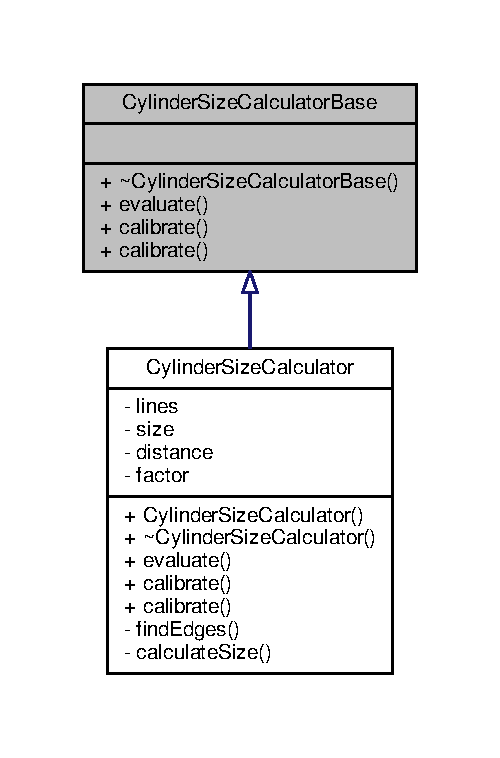
\includegraphics[width=240pt]{de/d05/class_cylinder_size_calculator_base__inherit__graph}
\end{center}
\end{figure}


Граф связей класса Cylinder\+Size\+Calculator\+Base\+:
\nopagebreak
\begin{figure}[H]
\begin{center}
\leavevmode
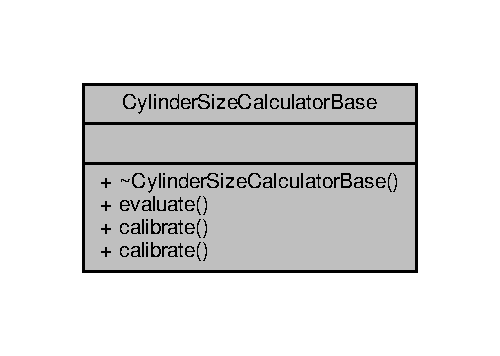
\includegraphics[width=240pt]{d3/dc3/class_cylinder_size_calculator_base__coll__graph}
\end{center}
\end{figure}
\subsection*{Открытые члены}
\begin{DoxyCompactItemize}
\item 
virtual \hyperlink{class_cylinder_size_calculator_base_acddec2ff7cfef169dc7df5ae3a2cc239}{$\sim$\+Cylinder\+Size\+Calculator\+Base} ()
\item 
virtual \hyperlink{class_cylinder_size}{Cylinder\+Size} \hyperlink{class_cylinder_size_calculator_base_adb5dd331f24a1c78b00266cb051f79ea}{evaluate} (const std\+::vector$<$ \hyperlink{class_line}{Line} $>$ \&lines)=0
\item 
virtual void \hyperlink{class_cylinder_size_calculator_base_ad37d6cd0b2746034294ed91e6ae2488e}{calibrate} (const std\+::vector$<$ \hyperlink{class_line}{Line} $>$ \&lines, float distance, float radius, float height)=0
\item 
virtual void \hyperlink{class_cylinder_size_calculator_base_a1713b5dbd13c49aeb2769cebaa24ebdb}{calibrate} (float daig, float diag\+Px)=0
\end{DoxyCompactItemize}


\subsection{Подробное описание}


См. определение в файле cylindersizecalculatorbase.\+h строка 10



\subsection{Конструктор(ы)}
\index{Cylinder\+Size\+Calculator\+Base@{Cylinder\+Size\+Calculator\+Base}!````~Cylinder\+Size\+Calculator\+Base@{$\sim$\+Cylinder\+Size\+Calculator\+Base}}
\index{````~Cylinder\+Size\+Calculator\+Base@{$\sim$\+Cylinder\+Size\+Calculator\+Base}!Cylinder\+Size\+Calculator\+Base@{Cylinder\+Size\+Calculator\+Base}}
\subsubsection[{\texorpdfstring{$\sim$\+Cylinder\+Size\+Calculator\+Base()}{~CylinderSizeCalculatorBase()}}]{\setlength{\rightskip}{0pt plus 5cm}Cylinder\+Size\+Calculator\+Base\+::$\sim$\+Cylinder\+Size\+Calculator\+Base (
\begin{DoxyParamCaption}
{}
\end{DoxyParamCaption}
)\hspace{0.3cm}{\ttfamily [virtual]}}\hypertarget{class_cylinder_size_calculator_base_acddec2ff7cfef169dc7df5ae3a2cc239}{}\label{class_cylinder_size_calculator_base_acddec2ff7cfef169dc7df5ae3a2cc239}


См. определение в файле cylindersizecalculatorbase.\+cpp строка 3



\subsection{Методы}
\index{Cylinder\+Size\+Calculator\+Base@{Cylinder\+Size\+Calculator\+Base}!calibrate@{calibrate}}
\index{calibrate@{calibrate}!Cylinder\+Size\+Calculator\+Base@{Cylinder\+Size\+Calculator\+Base}}
\subsubsection[{\texorpdfstring{calibrate(const std\+::vector$<$ Line $>$ \&lines, float distance, float radius, float height)=0}{calibrate(const std::vector< Line > &lines, float distance, float radius, float height)=0}}]{\setlength{\rightskip}{0pt plus 5cm}virtual void Cylinder\+Size\+Calculator\+Base\+::calibrate (
\begin{DoxyParamCaption}
\item[{const std\+::vector$<$ {\bf Line} $>$ \&}]{lines, }
\item[{float}]{distance, }
\item[{float}]{radius, }
\item[{float}]{height}
\end{DoxyParamCaption}
)\hspace{0.3cm}{\ttfamily [pure virtual]}}\hypertarget{class_cylinder_size_calculator_base_ad37d6cd0b2746034294ed91e6ae2488e}{}\label{class_cylinder_size_calculator_base_ad37d6cd0b2746034294ed91e6ae2488e}


Замещается в \hyperlink{class_cylinder_size_calculator_a411f74a0f0baa7c393fe53c36d957fd4}{Cylinder\+Size\+Calculator}.

\index{Cylinder\+Size\+Calculator\+Base@{Cylinder\+Size\+Calculator\+Base}!calibrate@{calibrate}}
\index{calibrate@{calibrate}!Cylinder\+Size\+Calculator\+Base@{Cylinder\+Size\+Calculator\+Base}}
\subsubsection[{\texorpdfstring{calibrate(float daig, float diag\+Px)=0}{calibrate(float daig, float diagPx)=0}}]{\setlength{\rightskip}{0pt plus 5cm}virtual void Cylinder\+Size\+Calculator\+Base\+::calibrate (
\begin{DoxyParamCaption}
\item[{float}]{daig, }
\item[{float}]{diag\+Px}
\end{DoxyParamCaption}
)\hspace{0.3cm}{\ttfamily [pure virtual]}}\hypertarget{class_cylinder_size_calculator_base_a1713b5dbd13c49aeb2769cebaa24ebdb}{}\label{class_cylinder_size_calculator_base_a1713b5dbd13c49aeb2769cebaa24ebdb}


Замещается в \hyperlink{class_cylinder_size_calculator_ace80de293c2d4626b65e83fcb0fcde54}{Cylinder\+Size\+Calculator}.

\index{Cylinder\+Size\+Calculator\+Base@{Cylinder\+Size\+Calculator\+Base}!evaluate@{evaluate}}
\index{evaluate@{evaluate}!Cylinder\+Size\+Calculator\+Base@{Cylinder\+Size\+Calculator\+Base}}
\subsubsection[{\texorpdfstring{evaluate(const std\+::vector$<$ Line $>$ \&lines)=0}{evaluate(const std::vector< Line > &lines)=0}}]{\setlength{\rightskip}{0pt plus 5cm}virtual {\bf Cylinder\+Size} Cylinder\+Size\+Calculator\+Base\+::evaluate (
\begin{DoxyParamCaption}
\item[{const std\+::vector$<$ {\bf Line} $>$ \&}]{lines}
\end{DoxyParamCaption}
)\hspace{0.3cm}{\ttfamily [pure virtual]}}\hypertarget{class_cylinder_size_calculator_base_adb5dd331f24a1c78b00266cb051f79ea}{}\label{class_cylinder_size_calculator_base_adb5dd331f24a1c78b00266cb051f79ea}


Замещается в \hyperlink{class_cylinder_size_calculator_a979a607bd694c5819355793d231c5df2}{Cylinder\+Size\+Calculator}.



Объявления и описания членов классов находятся в файлах\+:\begin{DoxyCompactItemize}
\item 
Projects/labs/course\+\_\+project\+\_\+cg/src/algorithm/\hyperlink{cylindersizecalculatorbase_8h}{cylindersizecalculatorbase.\+h}\item 
Projects/labs/course\+\_\+project\+\_\+cg/src/algorithm/\hyperlink{cylindersizecalculatorbase_8cpp}{cylindersizecalculatorbase.\+cpp}\end{DoxyCompactItemize}

\hypertarget{class_edge_detector}{}\section{Класс Edge\+Detector}
\label{class_edge_detector}\index{Edge\+Detector@{Edge\+Detector}}


{\ttfamily \#include $<$edgedetector.\+h$>$}



Граф наследования\+:Edge\+Detector\+:
\nopagebreak
\begin{figure}[H]
\begin{center}
\leavevmode
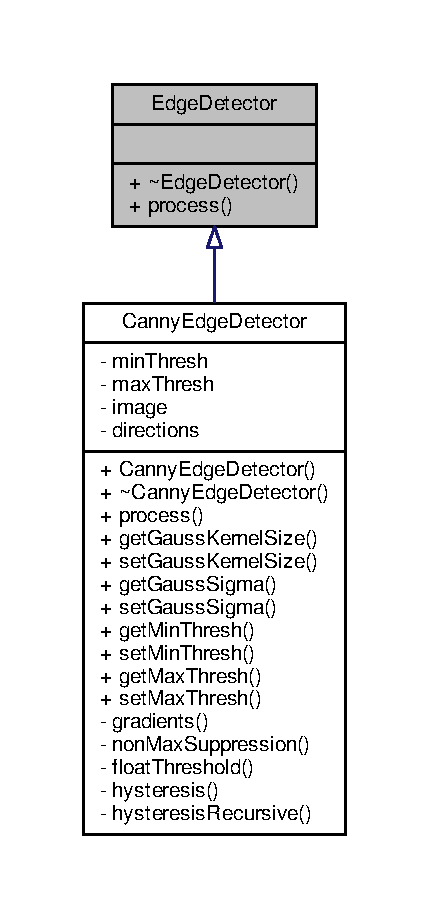
\includegraphics[width=206pt]{db/d47/class_edge_detector__inherit__graph}
\end{center}
\end{figure}


Граф связей класса Edge\+Detector\+:
\nopagebreak
\begin{figure}[H]
\begin{center}
\leavevmode
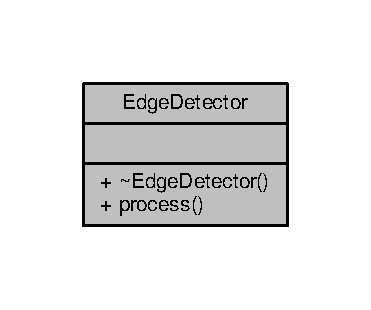
\includegraphics[width=178pt]{d3/dbb/class_edge_detector__coll__graph}
\end{center}
\end{figure}
\subsection*{Открытые члены}
\begin{DoxyCompactItemize}
\item 
virtual \hyperlink{class_edge_detector_a84d1668be5dd4052278a2cf86802746e}{$\sim$\+Edge\+Detector} ()
\item 
virtual void \hyperlink{class_edge_detector_aefa2d90e960e7dc3171bccadbed4a13e}{process} (\hyperlink{class_image}{Image} \&image)=0
\end{DoxyCompactItemize}


\subsection{Подробное описание}


См. определение в файле edgedetector.\+h строка 6



\subsection{Конструктор(ы)}
\index{Edge\+Detector@{Edge\+Detector}!````~Edge\+Detector@{$\sim$\+Edge\+Detector}}
\index{````~Edge\+Detector@{$\sim$\+Edge\+Detector}!Edge\+Detector@{Edge\+Detector}}
\subsubsection[{\texorpdfstring{$\sim$\+Edge\+Detector()}{~EdgeDetector()}}]{\setlength{\rightskip}{0pt plus 5cm}Edge\+Detector\+::$\sim$\+Edge\+Detector (
\begin{DoxyParamCaption}
{}
\end{DoxyParamCaption}
)\hspace{0.3cm}{\ttfamily [virtual]}}\hypertarget{class_edge_detector_a84d1668be5dd4052278a2cf86802746e}{}\label{class_edge_detector_a84d1668be5dd4052278a2cf86802746e}


См. определение в файле edgedetector.\+cpp строка 4



\subsection{Методы}
\index{Edge\+Detector@{Edge\+Detector}!process@{process}}
\index{process@{process}!Edge\+Detector@{Edge\+Detector}}
\subsubsection[{\texorpdfstring{process(\+Image \&image)=0}{process(Image &image)=0}}]{\setlength{\rightskip}{0pt plus 5cm}virtual void Edge\+Detector\+::process (
\begin{DoxyParamCaption}
\item[{{\bf Image} \&}]{image}
\end{DoxyParamCaption}
)\hspace{0.3cm}{\ttfamily [pure virtual]}}\hypertarget{class_edge_detector_aefa2d90e960e7dc3171bccadbed4a13e}{}\label{class_edge_detector_aefa2d90e960e7dc3171bccadbed4a13e}


Замещается в \hyperlink{class_canny_edge_detector_ae97e095e14e43d763a8fc2563f6e9a87}{Canny\+Edge\+Detector}.



Объявления и описания членов классов находятся в файлах\+:\begin{DoxyCompactItemize}
\item 
Projects/labs/course\+\_\+project\+\_\+cg/src/algorithm/edgedetector/\hyperlink{edgedetector_8h}{edgedetector.\+h}\item 
Projects/labs/course\+\_\+project\+\_\+cg/src/algorithm/edgedetector/\hyperlink{edgedetector_8cpp}{edgedetector.\+cpp}\end{DoxyCompactItemize}

\hypertarget{class_gaussian_blur}{}\section{Класс Gaussian\+Blur}
\label{class_gaussian_blur}\index{Gaussian\+Blur@{Gaussian\+Blur}}


{\ttfamily \#include $<$gaussianblur.\+h$>$}



Граф наследования\+:Gaussian\+Blur\+:
\nopagebreak
\begin{figure}[H]
\begin{center}
\leavevmode
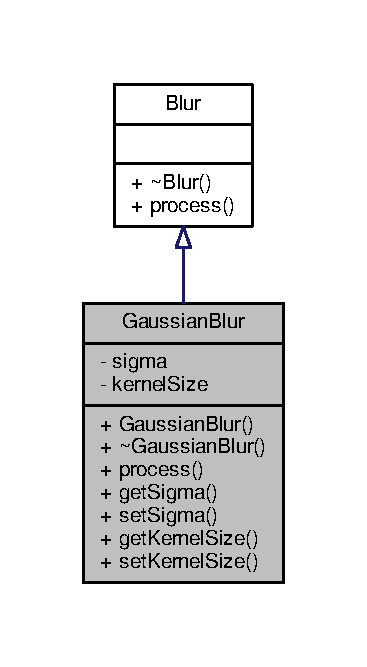
\includegraphics[width=176pt]{d4/d1f/class_gaussian_blur__inherit__graph}
\end{center}
\end{figure}


Граф связей класса Gaussian\+Blur\+:
\nopagebreak
\begin{figure}[H]
\begin{center}
\leavevmode
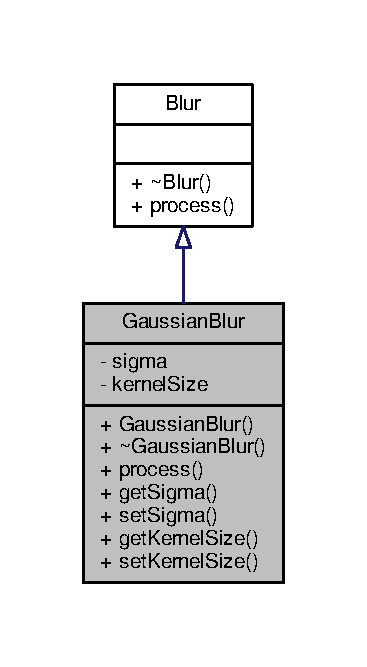
\includegraphics[width=176pt]{d0/df8/class_gaussian_blur__coll__graph}
\end{center}
\end{figure}
\subsection*{Открытые члены}
\begin{DoxyCompactItemize}
\item 
\hyperlink{class_gaussian_blur_a673756a20ccaacc46de77e6c355276d2}{Gaussian\+Blur} (float \hyperlink{class_gaussian_blur_ab43cc1fff30574e2e04876fda4a55441}{sigma}=1.\+4, \hyperlink{number_8h_adde6aaee8457bee49c2a92621fe22b79}{uint8} \hyperlink{class_gaussian_blur_ab71bceac5e6b8f3f2d2868f40ff0f80b}{kernel\+Size}=3)
\item 
virtual \hyperlink{class_gaussian_blur_a881b005db6cc737bf1d6a8ab3d32c6b1}{$\sim$\+Gaussian\+Blur} ()
\item 
virtual void \hyperlink{class_gaussian_blur_a6af6684bdf5e86e5c9a79fe1f3a8c183}{process} (\hyperlink{class_image}{Image} \&image)
\item 
float \hyperlink{class_gaussian_blur_a409c05410353b2bb7abfa0ac0e7e2279}{get\+Sigma} () const 
\item 
void \hyperlink{class_gaussian_blur_aa4203a493fb56be7dec2af1e90667af1}{set\+Sigma} (float value)
\item 
\hyperlink{number_8h_adde6aaee8457bee49c2a92621fe22b79}{uint8} \hyperlink{class_gaussian_blur_a47c6c015416e7f0770d2990beb85a48c}{get\+Kernel\+Size} () const 
\item 
void \hyperlink{class_gaussian_blur_ad8b1e0c74123f050daa79d20c3636064}{set\+Kernel\+Size} (const \hyperlink{number_8h_adde6aaee8457bee49c2a92621fe22b79}{uint8} \&value)
\end{DoxyCompactItemize}
\subsection*{Закрытые данные}
\begin{DoxyCompactItemize}
\item 
float \hyperlink{class_gaussian_blur_ab43cc1fff30574e2e04876fda4a55441}{sigma}
\item 
\hyperlink{number_8h_adde6aaee8457bee49c2a92621fe22b79}{uint8} \hyperlink{class_gaussian_blur_ab71bceac5e6b8f3f2d2868f40ff0f80b}{kernel\+Size}
\end{DoxyCompactItemize}


\subsection{Подробное описание}


См. определение в файле gaussianblur.\+h строка 7



\subsection{Конструктор(ы)}
\index{Gaussian\+Blur@{Gaussian\+Blur}!Gaussian\+Blur@{Gaussian\+Blur}}
\index{Gaussian\+Blur@{Gaussian\+Blur}!Gaussian\+Blur@{Gaussian\+Blur}}
\subsubsection[{\texorpdfstring{Gaussian\+Blur(float sigma=1.\+4, uint8 kernel\+Size=3)}{GaussianBlur(float sigma=1.4, uint8 kernelSize=3)}}]{\setlength{\rightskip}{0pt plus 5cm}Gaussian\+Blur\+::\+Gaussian\+Blur (
\begin{DoxyParamCaption}
\item[{float}]{sigma = {\ttfamily 1.4}, }
\item[{{\bf uint8}}]{kernel\+Size = {\ttfamily 3}}
\end{DoxyParamCaption}
)}\hypertarget{class_gaussian_blur_a673756a20ccaacc46de77e6c355276d2}{}\label{class_gaussian_blur_a673756a20ccaacc46de77e6c355276d2}


См. определение в файле gaussianblur.\+cpp строка 6

\index{Gaussian\+Blur@{Gaussian\+Blur}!````~Gaussian\+Blur@{$\sim$\+Gaussian\+Blur}}
\index{````~Gaussian\+Blur@{$\sim$\+Gaussian\+Blur}!Gaussian\+Blur@{Gaussian\+Blur}}
\subsubsection[{\texorpdfstring{$\sim$\+Gaussian\+Blur()}{~GaussianBlur()}}]{\setlength{\rightskip}{0pt plus 5cm}Gaussian\+Blur\+::$\sim$\+Gaussian\+Blur (
\begin{DoxyParamCaption}
{}
\end{DoxyParamCaption}
)\hspace{0.3cm}{\ttfamily [virtual]}}\hypertarget{class_gaussian_blur_a881b005db6cc737bf1d6a8ab3d32c6b1}{}\label{class_gaussian_blur_a881b005db6cc737bf1d6a8ab3d32c6b1}


См. определение в файле gaussianblur.\+cpp строка 12



\subsection{Методы}
\index{Gaussian\+Blur@{Gaussian\+Blur}!get\+Kernel\+Size@{get\+Kernel\+Size}}
\index{get\+Kernel\+Size@{get\+Kernel\+Size}!Gaussian\+Blur@{Gaussian\+Blur}}
\subsubsection[{\texorpdfstring{get\+Kernel\+Size() const }{getKernelSize() const }}]{\setlength{\rightskip}{0pt plus 5cm}{\bf uint8} Gaussian\+Blur\+::get\+Kernel\+Size (
\begin{DoxyParamCaption}
{}
\end{DoxyParamCaption}
) const}\hypertarget{class_gaussian_blur_a47c6c015416e7f0770d2990beb85a48c}{}\label{class_gaussian_blur_a47c6c015416e7f0770d2990beb85a48c}


См. определение в файле gaussianblur.\+cpp строка 83

\index{Gaussian\+Blur@{Gaussian\+Blur}!get\+Sigma@{get\+Sigma}}
\index{get\+Sigma@{get\+Sigma}!Gaussian\+Blur@{Gaussian\+Blur}}
\subsubsection[{\texorpdfstring{get\+Sigma() const }{getSigma() const }}]{\setlength{\rightskip}{0pt plus 5cm}float Gaussian\+Blur\+::get\+Sigma (
\begin{DoxyParamCaption}
{}
\end{DoxyParamCaption}
) const}\hypertarget{class_gaussian_blur_a409c05410353b2bb7abfa0ac0e7e2279}{}\label{class_gaussian_blur_a409c05410353b2bb7abfa0ac0e7e2279}


См. определение в файле gaussianblur.\+cpp строка 73

\index{Gaussian\+Blur@{Gaussian\+Blur}!process@{process}}
\index{process@{process}!Gaussian\+Blur@{Gaussian\+Blur}}
\subsubsection[{\texorpdfstring{process(\+Image \&image)}{process(Image &image)}}]{\setlength{\rightskip}{0pt plus 5cm}void Gaussian\+Blur\+::process (
\begin{DoxyParamCaption}
\item[{{\bf Image} \&}]{image}
\end{DoxyParamCaption}
)\hspace{0.3cm}{\ttfamily [virtual]}}\hypertarget{class_gaussian_blur_a6af6684bdf5e86e5c9a79fe1f3a8c183}{}\label{class_gaussian_blur_a6af6684bdf5e86e5c9a79fe1f3a8c183}


Замещает \hyperlink{class_blur_a675fd2caa4a262e8140bdff64912bab4}{Blur}.



См. определение в файле gaussianblur.\+cpp строка 16

\index{Gaussian\+Blur@{Gaussian\+Blur}!set\+Kernel\+Size@{set\+Kernel\+Size}}
\index{set\+Kernel\+Size@{set\+Kernel\+Size}!Gaussian\+Blur@{Gaussian\+Blur}}
\subsubsection[{\texorpdfstring{set\+Kernel\+Size(const uint8 \&value)}{setKernelSize(const uint8 &value)}}]{\setlength{\rightskip}{0pt plus 5cm}void Gaussian\+Blur\+::set\+Kernel\+Size (
\begin{DoxyParamCaption}
\item[{const {\bf uint8} \&}]{value}
\end{DoxyParamCaption}
)}\hypertarget{class_gaussian_blur_ad8b1e0c74123f050daa79d20c3636064}{}\label{class_gaussian_blur_ad8b1e0c74123f050daa79d20c3636064}


См. определение в файле gaussianblur.\+cpp строка 88

\index{Gaussian\+Blur@{Gaussian\+Blur}!set\+Sigma@{set\+Sigma}}
\index{set\+Sigma@{set\+Sigma}!Gaussian\+Blur@{Gaussian\+Blur}}
\subsubsection[{\texorpdfstring{set\+Sigma(float value)}{setSigma(float value)}}]{\setlength{\rightskip}{0pt plus 5cm}void Gaussian\+Blur\+::set\+Sigma (
\begin{DoxyParamCaption}
\item[{float}]{value}
\end{DoxyParamCaption}
)}\hypertarget{class_gaussian_blur_aa4203a493fb56be7dec2af1e90667af1}{}\label{class_gaussian_blur_aa4203a493fb56be7dec2af1e90667af1}


См. определение в файле gaussianblur.\+cpp строка 78



\subsection{Данные класса}
\index{Gaussian\+Blur@{Gaussian\+Blur}!kernel\+Size@{kernel\+Size}}
\index{kernel\+Size@{kernel\+Size}!Gaussian\+Blur@{Gaussian\+Blur}}
\subsubsection[{\texorpdfstring{kernel\+Size}{kernelSize}}]{\setlength{\rightskip}{0pt plus 5cm}{\bf uint8} Gaussian\+Blur\+::kernel\+Size\hspace{0.3cm}{\ttfamily [private]}}\hypertarget{class_gaussian_blur_ab71bceac5e6b8f3f2d2868f40ff0f80b}{}\label{class_gaussian_blur_ab71bceac5e6b8f3f2d2868f40ff0f80b}


См. определение в файле gaussianblur.\+h строка 22

\index{Gaussian\+Blur@{Gaussian\+Blur}!sigma@{sigma}}
\index{sigma@{sigma}!Gaussian\+Blur@{Gaussian\+Blur}}
\subsubsection[{\texorpdfstring{sigma}{sigma}}]{\setlength{\rightskip}{0pt plus 5cm}float Gaussian\+Blur\+::sigma\hspace{0.3cm}{\ttfamily [private]}}\hypertarget{class_gaussian_blur_ab43cc1fff30574e2e04876fda4a55441}{}\label{class_gaussian_blur_ab43cc1fff30574e2e04876fda4a55441}


См. определение в файле gaussianblur.\+h строка 21



Объявления и описания членов классов находятся в файлах\+:\begin{DoxyCompactItemize}
\item 
Projects/labs/course\+\_\+project\+\_\+cg/src/algorithm/blur/\hyperlink{gaussianblur_8h}{gaussianblur.\+h}\item 
Projects/labs/course\+\_\+project\+\_\+cg/src/algorithm/blur/\hyperlink{gaussianblur_8cpp}{gaussianblur.\+cpp}\end{DoxyCompactItemize}

\hypertarget{class_grayscale_image}{}\section{Класс Grayscale\+Image}
\label{class_grayscale_image}\index{Grayscale\+Image@{Grayscale\+Image}}


{\ttfamily \#include $<$grayscaleimage.\+h$>$}



Граф наследования\+:Grayscale\+Image\+:
\nopagebreak
\begin{figure}[H]
\begin{center}
\leavevmode
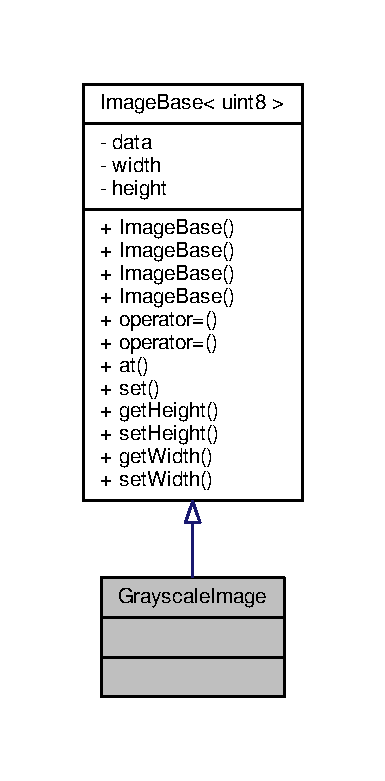
\includegraphics[width=185pt]{d2/dd8/class_grayscale_image__inherit__graph}
\end{center}
\end{figure}


Граф связей класса Grayscale\+Image\+:
\nopagebreak
\begin{figure}[H]
\begin{center}
\leavevmode
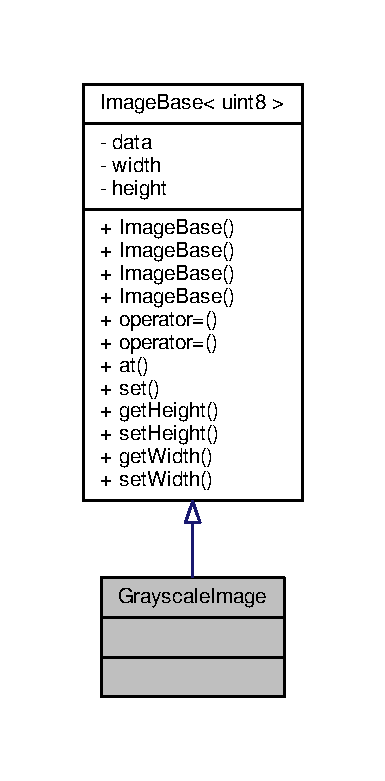
\includegraphics[width=185pt]{d6/d4d/class_grayscale_image__coll__graph}
\end{center}
\end{figure}
\subsection*{Друзья}
\begin{DoxyCompactItemize}
\item 
class \hyperlink{class_grayscale_image_a683b929065aaead03ccce450a7b4ab30}{Image\+Converter}
\item 
class \hyperlink{class_grayscale_image_a655e20b76703bb6a4e6ecd9ed4a5d9ed}{Grayscale\+Converter}
\end{DoxyCompactItemize}
\subsection*{Дополнительные унаследованные члены}


\subsection{Подробное описание}


См. определение в файле grayscaleimage.\+h строка 14



\subsection{Документация по друзьям класса и функциям, относящимся к классу}
\index{Grayscale\+Image@{Grayscale\+Image}!Grayscale\+Converter@{Grayscale\+Converter}}
\index{Grayscale\+Converter@{Grayscale\+Converter}!Grayscale\+Image@{Grayscale\+Image}}
\subsubsection[{\texorpdfstring{Grayscale\+Converter}{GrayscaleConverter}}]{\setlength{\rightskip}{0pt plus 5cm}friend class Grayscale\+Converter\hspace{0.3cm}{\ttfamily [friend]}}\hypertarget{class_grayscale_image_a655e20b76703bb6a4e6ecd9ed4a5d9ed}{}\label{class_grayscale_image_a655e20b76703bb6a4e6ecd9ed4a5d9ed}


См. определение в файле grayscaleimage.\+h строка 20

\index{Grayscale\+Image@{Grayscale\+Image}!Image\+Converter@{Image\+Converter}}
\index{Image\+Converter@{Image\+Converter}!Grayscale\+Image@{Grayscale\+Image}}
\subsubsection[{\texorpdfstring{Image\+Converter}{ImageConverter}}]{\setlength{\rightskip}{0pt plus 5cm}friend class {\bf Image\+Converter}\hspace{0.3cm}{\ttfamily [friend]}}\hypertarget{class_grayscale_image_a683b929065aaead03ccce450a7b4ab30}{}\label{class_grayscale_image_a683b929065aaead03ccce450a7b4ab30}


См. определение в файле grayscaleimage.\+h строка 19



Объявления и описания членов класса находятся в файле\+:\begin{DoxyCompactItemize}
\item 
Projects/labs/course\+\_\+project\+\_\+cg/src/image/\hyperlink{grayscaleimage_8h}{grayscaleimage.\+h}\end{DoxyCompactItemize}

\hypertarget{class_homogeneous_vertex_converter}{}\section{Класс Homogeneous\+Vertex\+Converter}
\label{class_homogeneous_vertex_converter}\index{Homogeneous\+Vertex\+Converter@{Homogeneous\+Vertex\+Converter}}


{\ttfamily \#include $<$homogeneousvertex.\+h$>$}



Граф связей класса Homogeneous\+Vertex\+Converter\+:
\nopagebreak
\begin{figure}[H]
\begin{center}
\leavevmode
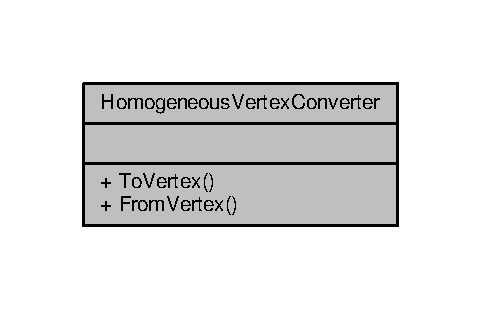
\includegraphics[width=231pt]{d9/d45/class_homogeneous_vertex_converter__coll__graph}
\end{center}
\end{figure}
\subsection*{Открытые статические члены}
\begin{DoxyCompactItemize}
\item 
static \hyperlink{vec3_8h_a221ad8ea4d9be4111628ee1ca22ee3ba}{Vec3} \hyperlink{class_homogeneous_vertex_converter_a5ee9db87aeed48aec688c3ce53ae4e4c}{To\+Vertex} (const \hyperlink{homogeneousvertex_8h_ac57a7e4c1ca5e8ae47858d4ae8e7120d}{Homogeneous\+Vertex} \&hvec)
\item 
static \hyperlink{homogeneousvertex_8h_ac57a7e4c1ca5e8ae47858d4ae8e7120d}{Homogeneous\+Vertex} \hyperlink{class_homogeneous_vertex_converter_a2e43c599f3a88f27316d098548430978}{From\+Vertex} (const \hyperlink{vec3_8h_a221ad8ea4d9be4111628ee1ca22ee3ba}{Vec3} \&vec)
\end{DoxyCompactItemize}


\subsection{Подробное описание}


См. определение в файле homogeneousvertex.\+h строка 9



\subsection{Методы}
\index{Homogeneous\+Vertex\+Converter@{Homogeneous\+Vertex\+Converter}!From\+Vertex@{From\+Vertex}}
\index{From\+Vertex@{From\+Vertex}!Homogeneous\+Vertex\+Converter@{Homogeneous\+Vertex\+Converter}}
\subsubsection[{\texorpdfstring{From\+Vertex(const Vec3 \&vec)}{FromVertex(const Vec3 &vec)}}]{\setlength{\rightskip}{0pt plus 5cm}{\bf Homogeneous\+Vertex} Homogeneous\+Vertex\+Converter\+::\+From\+Vertex (
\begin{DoxyParamCaption}
\item[{const {\bf Vec3} \&}]{vec}
\end{DoxyParamCaption}
)\hspace{0.3cm}{\ttfamily [static]}}\hypertarget{class_homogeneous_vertex_converter_a2e43c599f3a88f27316d098548430978}{}\label{class_homogeneous_vertex_converter_a2e43c599f3a88f27316d098548430978}


См. определение в файле homogeneousvertex.\+cpp строка 13

\index{Homogeneous\+Vertex\+Converter@{Homogeneous\+Vertex\+Converter}!To\+Vertex@{To\+Vertex}}
\index{To\+Vertex@{To\+Vertex}!Homogeneous\+Vertex\+Converter@{Homogeneous\+Vertex\+Converter}}
\subsubsection[{\texorpdfstring{To\+Vertex(const Homogeneous\+Vertex \&hvec)}{ToVertex(const HomogeneousVertex &hvec)}}]{\setlength{\rightskip}{0pt plus 5cm}{\bf Vec3} Homogeneous\+Vertex\+Converter\+::\+To\+Vertex (
\begin{DoxyParamCaption}
\item[{const {\bf Homogeneous\+Vertex} \&}]{hvec}
\end{DoxyParamCaption}
)\hspace{0.3cm}{\ttfamily [static]}}\hypertarget{class_homogeneous_vertex_converter_a5ee9db87aeed48aec688c3ce53ae4e4c}{}\label{class_homogeneous_vertex_converter_a5ee9db87aeed48aec688c3ce53ae4e4c}


См. определение в файле homogeneousvertex.\+cpp строка 5



Объявления и описания членов классов находятся в файлах\+:\begin{DoxyCompactItemize}
\item 
Projects/labs/course\+\_\+project\+\_\+cg/src/math/\hyperlink{homogeneousvertex_8h}{homogeneousvertex.\+h}\item 
Projects/labs/course\+\_\+project\+\_\+cg/src/math/\hyperlink{homogeneousvertex_8cpp}{homogeneousvertex.\+cpp}\end{DoxyCompactItemize}

\hypertarget{class_hough_transform}{}\section{Класс Hough\+Transform}
\label{class_hough_transform}\index{Hough\+Transform@{Hough\+Transform}}


{\ttfamily \#include $<$houghtransform.\+h$>$}



Граф наследования\+:Hough\+Transform\+:
\nopagebreak
\begin{figure}[H]
\begin{center}
\leavevmode
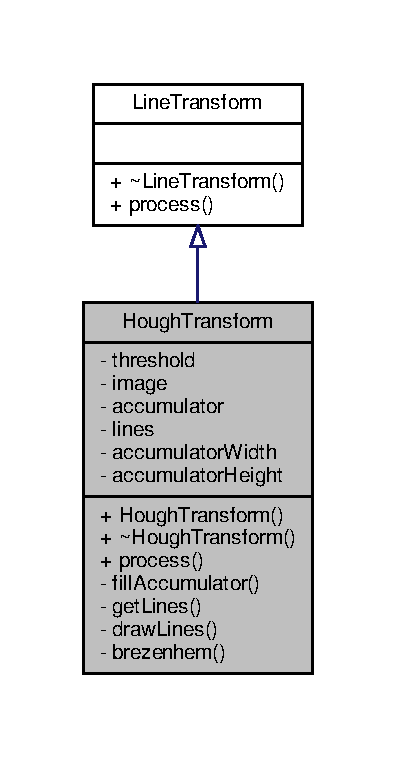
\includegraphics[width=190pt]{d4/d8d/class_hough_transform__inherit__graph}
\end{center}
\end{figure}


Граф связей класса Hough\+Transform\+:
\nopagebreak
\begin{figure}[H]
\begin{center}
\leavevmode
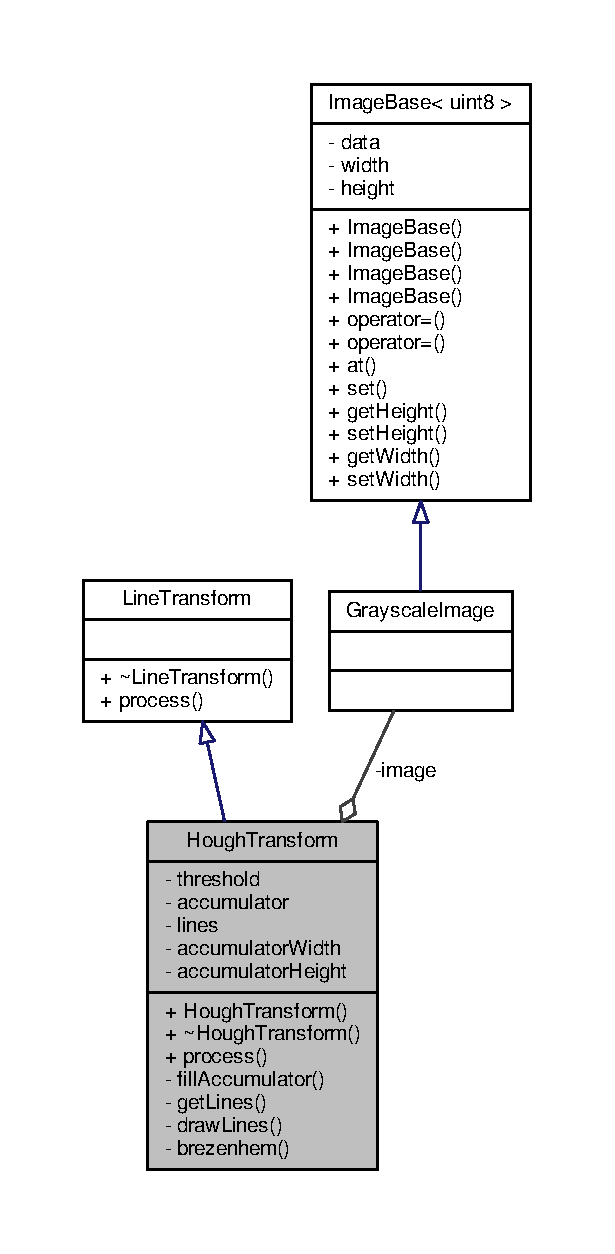
\includegraphics[height=550pt]{dc/d45/class_hough_transform__coll__graph}
\end{center}
\end{figure}
\subsection*{Открытые члены}
\begin{DoxyCompactItemize}
\item 
\hyperlink{class_hough_transform_aa0129504dee413d479db4f400047e525}{Hough\+Transform} (\hyperlink{number_8h_a1134b580f8da4de94ca6b1de4d37975e}{uint32} \hyperlink{class_hough_transform_aa9de5274a062b1725689fbbc6f0799f7}{threshold}=50)
\item 
virtual \hyperlink{class_hough_transform_a1bcf9b1138d21afd88db2a96873ff741}{$\sim$\+Hough\+Transform} ()
\item 
virtual std\+::vector$<$ \hyperlink{class_line}{Line} $>$ \hyperlink{class_hough_transform_ab10d9e25f492521d6436701107b93fac}{process} (\hyperlink{class_image}{Image} \&\hyperlink{class_hough_transform_a0fe725cb1f0e3078096c3d7e9dee85f7}{image})
\end{DoxyCompactItemize}
\subsection*{Закрытые типы}
\begin{DoxyCompactItemize}
\item 
using \hyperlink{class_hough_transform_acca3cb75c9e1a69b38a0ef97a6b3e6ae}{Points} = std\+::vector$<$ \hyperlink{vec2_8h_a056bf34213a36593f50f333d7653fe1c}{Vec2} $>$
\end{DoxyCompactItemize}
\subsection*{Закрытые члены}
\begin{DoxyCompactItemize}
\item 
void \hyperlink{class_hough_transform_a9cbe414b810e761a1b776d268fd13fa5}{fill\+Accumulator} ()
\item 
void \hyperlink{class_hough_transform_a7292b312db2f7bbf90d52c755b9de28a}{get\+Lines} ()
\item 
void \hyperlink{class_hough_transform_a0eee01dc4d43dc5545b832513aeb6ff4}{draw\+Lines} (\hyperlink{class_image}{Image} \&color)
\item 
void \hyperlink{class_hough_transform_a2ea26ee041bf7dd1e50616d3411138cf}{brezenhem} (\hyperlink{class_image}{Image} \&color, const \hyperlink{class_line}{Line} \&line)
\end{DoxyCompactItemize}
\subsection*{Закрытые данные}
\begin{DoxyCompactItemize}
\item 
\hyperlink{number_8h_a1134b580f8da4de94ca6b1de4d37975e}{uint32} \hyperlink{class_hough_transform_aa9de5274a062b1725689fbbc6f0799f7}{threshold}
\item 
\hyperlink{class_grayscale_image}{Grayscale\+Image} \hyperlink{class_hough_transform_a0fe725cb1f0e3078096c3d7e9dee85f7}{image}
\item 
std\+::vector$<$ \hyperlink{class_hough_transform_acca3cb75c9e1a69b38a0ef97a6b3e6ae}{Points} $>$ \hyperlink{class_hough_transform_aaa271ada2195b2f0dba1a4611648fc2f}{accumulator}
\item 
std\+::vector$<$ \hyperlink{class_line}{Line} $>$ \hyperlink{class_hough_transform_abb2e77efd0688f3ea508c5f51b480f22}{lines}
\item 
\hyperlink{number_8h_a1134b580f8da4de94ca6b1de4d37975e}{uint32} \hyperlink{class_hough_transform_a1c2b5fa2274a44848f8737f396397137}{accumulator\+Width}
\item 
\hyperlink{number_8h_a1134b580f8da4de94ca6b1de4d37975e}{uint32} \hyperlink{class_hough_transform_aee054a46260dc381123d158617c0e7dc}{accumulator\+Height}
\end{DoxyCompactItemize}


\subsection{Подробное описание}


См. определение в файле houghtransform.\+h строка 11



\subsection{Определения типов}
\index{Hough\+Transform@{Hough\+Transform}!Points@{Points}}
\index{Points@{Points}!Hough\+Transform@{Hough\+Transform}}
\subsubsection[{\texorpdfstring{Points}{Points}}]{\setlength{\rightskip}{0pt plus 5cm}using {\bf Hough\+Transform\+::\+Points} =  std\+::vector$<${\bf Vec2}$>$\hspace{0.3cm}{\ttfamily [private]}}\hypertarget{class_hough_transform_acca3cb75c9e1a69b38a0ef97a6b3e6ae}{}\label{class_hough_transform_acca3cb75c9e1a69b38a0ef97a6b3e6ae}


См. определение в файле houghtransform.\+h строка 14



\subsection{Конструктор(ы)}
\index{Hough\+Transform@{Hough\+Transform}!Hough\+Transform@{Hough\+Transform}}
\index{Hough\+Transform@{Hough\+Transform}!Hough\+Transform@{Hough\+Transform}}
\subsubsection[{\texorpdfstring{Hough\+Transform(uint32 threshold=50)}{HoughTransform(uint32 threshold=50)}}]{\setlength{\rightskip}{0pt plus 5cm}Hough\+Transform\+::\+Hough\+Transform (
\begin{DoxyParamCaption}
\item[{{\bf uint32}}]{threshold = {\ttfamily 50}}
\end{DoxyParamCaption}
)}\hypertarget{class_hough_transform_aa0129504dee413d479db4f400047e525}{}\label{class_hough_transform_aa0129504dee413d479db4f400047e525}


См. определение в файле houghtransform.\+cpp строка 7

\index{Hough\+Transform@{Hough\+Transform}!````~Hough\+Transform@{$\sim$\+Hough\+Transform}}
\index{````~Hough\+Transform@{$\sim$\+Hough\+Transform}!Hough\+Transform@{Hough\+Transform}}
\subsubsection[{\texorpdfstring{$\sim$\+Hough\+Transform()}{~HoughTransform()}}]{\setlength{\rightskip}{0pt plus 5cm}Hough\+Transform\+::$\sim$\+Hough\+Transform (
\begin{DoxyParamCaption}
{}
\end{DoxyParamCaption}
)\hspace{0.3cm}{\ttfamily [virtual]}}\hypertarget{class_hough_transform_a1bcf9b1138d21afd88db2a96873ff741}{}\label{class_hough_transform_a1bcf9b1138d21afd88db2a96873ff741}


См. определение в файле houghtransform.\+cpp строка 12



\subsection{Методы}
\index{Hough\+Transform@{Hough\+Transform}!brezenhem@{brezenhem}}
\index{brezenhem@{brezenhem}!Hough\+Transform@{Hough\+Transform}}
\subsubsection[{\texorpdfstring{brezenhem(\+Image \&color, const Line \&line)}{brezenhem(Image &color, const Line &line)}}]{\setlength{\rightskip}{0pt plus 5cm}void Hough\+Transform\+::brezenhem (
\begin{DoxyParamCaption}
\item[{{\bf Image} \&}]{color, }
\item[{const {\bf Line} \&}]{line}
\end{DoxyParamCaption}
)\hspace{0.3cm}{\ttfamily [private]}}\hypertarget{class_hough_transform_a2ea26ee041bf7dd1e50616d3411138cf}{}\label{class_hough_transform_a2ea26ee041bf7dd1e50616d3411138cf}


См. определение в файле houghtransform.\+cpp строка 139

\index{Hough\+Transform@{Hough\+Transform}!draw\+Lines@{draw\+Lines}}
\index{draw\+Lines@{draw\+Lines}!Hough\+Transform@{Hough\+Transform}}
\subsubsection[{\texorpdfstring{draw\+Lines(\+Image \&color)}{drawLines(Image &color)}}]{\setlength{\rightskip}{0pt plus 5cm}void Hough\+Transform\+::draw\+Lines (
\begin{DoxyParamCaption}
\item[{{\bf Image} \&}]{color}
\end{DoxyParamCaption}
)\hspace{0.3cm}{\ttfamily [private]}}\hypertarget{class_hough_transform_a0eee01dc4d43dc5545b832513aeb6ff4}{}\label{class_hough_transform_a0eee01dc4d43dc5545b832513aeb6ff4}


См. определение в файле houghtransform.\+cpp строка 131

\index{Hough\+Transform@{Hough\+Transform}!fill\+Accumulator@{fill\+Accumulator}}
\index{fill\+Accumulator@{fill\+Accumulator}!Hough\+Transform@{Hough\+Transform}}
\subsubsection[{\texorpdfstring{fill\+Accumulator()}{fillAccumulator()}}]{\setlength{\rightskip}{0pt plus 5cm}void Hough\+Transform\+::fill\+Accumulator (
\begin{DoxyParamCaption}
{}
\end{DoxyParamCaption}
)\hspace{0.3cm}{\ttfamily [private]}}\hypertarget{class_hough_transform_a9cbe414b810e761a1b776d268fd13fa5}{}\label{class_hough_transform_a9cbe414b810e761a1b776d268fd13fa5}


См. определение в файле houghtransform.\+cpp строка 29

\index{Hough\+Transform@{Hough\+Transform}!get\+Lines@{get\+Lines}}
\index{get\+Lines@{get\+Lines}!Hough\+Transform@{Hough\+Transform}}
\subsubsection[{\texorpdfstring{get\+Lines()}{getLines()}}]{\setlength{\rightskip}{0pt plus 5cm}void Hough\+Transform\+::get\+Lines (
\begin{DoxyParamCaption}
{}
\end{DoxyParamCaption}
)\hspace{0.3cm}{\ttfamily [private]}}\hypertarget{class_hough_transform_a7292b312db2f7bbf90d52c755b9de28a}{}\label{class_hough_transform_a7292b312db2f7bbf90d52c755b9de28a}


См. определение в файле houghtransform.\+cpp строка 58

\index{Hough\+Transform@{Hough\+Transform}!process@{process}}
\index{process@{process}!Hough\+Transform@{Hough\+Transform}}
\subsubsection[{\texorpdfstring{process(\+Image \&image)}{process(Image &image)}}]{\setlength{\rightskip}{0pt plus 5cm}std\+::vector$<$ {\bf Line} $>$ Hough\+Transform\+::process (
\begin{DoxyParamCaption}
\item[{{\bf Image} \&}]{image}
\end{DoxyParamCaption}
)\hspace{0.3cm}{\ttfamily [virtual]}}\hypertarget{class_hough_transform_ab10d9e25f492521d6436701107b93fac}{}\label{class_hough_transform_ab10d9e25f492521d6436701107b93fac}


Замещает \hyperlink{class_line_transform_a391ea9da214224bd3fe428a41c271761}{Line\+Transform}.



См. определение в файле houghtransform.\+cpp строка 16



\subsection{Данные класса}
\index{Hough\+Transform@{Hough\+Transform}!accumulator@{accumulator}}
\index{accumulator@{accumulator}!Hough\+Transform@{Hough\+Transform}}
\subsubsection[{\texorpdfstring{accumulator}{accumulator}}]{\setlength{\rightskip}{0pt plus 5cm}std\+::vector$<${\bf Points}$>$ Hough\+Transform\+::accumulator\hspace{0.3cm}{\ttfamily [private]}}\hypertarget{class_hough_transform_aaa271ada2195b2f0dba1a4611648fc2f}{}\label{class_hough_transform_aaa271ada2195b2f0dba1a4611648fc2f}


См. определение в файле houghtransform.\+h строка 32

\index{Hough\+Transform@{Hough\+Transform}!accumulator\+Height@{accumulator\+Height}}
\index{accumulator\+Height@{accumulator\+Height}!Hough\+Transform@{Hough\+Transform}}
\subsubsection[{\texorpdfstring{accumulator\+Height}{accumulatorHeight}}]{\setlength{\rightskip}{0pt plus 5cm}{\bf uint32} Hough\+Transform\+::accumulator\+Height\hspace{0.3cm}{\ttfamily [private]}}\hypertarget{class_hough_transform_aee054a46260dc381123d158617c0e7dc}{}\label{class_hough_transform_aee054a46260dc381123d158617c0e7dc}


См. определение в файле houghtransform.\+h строка 34

\index{Hough\+Transform@{Hough\+Transform}!accumulator\+Width@{accumulator\+Width}}
\index{accumulator\+Width@{accumulator\+Width}!Hough\+Transform@{Hough\+Transform}}
\subsubsection[{\texorpdfstring{accumulator\+Width}{accumulatorWidth}}]{\setlength{\rightskip}{0pt plus 5cm}{\bf uint32} Hough\+Transform\+::accumulator\+Width\hspace{0.3cm}{\ttfamily [private]}}\hypertarget{class_hough_transform_a1c2b5fa2274a44848f8737f396397137}{}\label{class_hough_transform_a1c2b5fa2274a44848f8737f396397137}


См. определение в файле houghtransform.\+h строка 34

\index{Hough\+Transform@{Hough\+Transform}!image@{image}}
\index{image@{image}!Hough\+Transform@{Hough\+Transform}}
\subsubsection[{\texorpdfstring{image}{image}}]{\setlength{\rightskip}{0pt plus 5cm}{\bf Grayscale\+Image} Hough\+Transform\+::image\hspace{0.3cm}{\ttfamily [private]}}\hypertarget{class_hough_transform_a0fe725cb1f0e3078096c3d7e9dee85f7}{}\label{class_hough_transform_a0fe725cb1f0e3078096c3d7e9dee85f7}


См. определение в файле houghtransform.\+h строка 30

\index{Hough\+Transform@{Hough\+Transform}!lines@{lines}}
\index{lines@{lines}!Hough\+Transform@{Hough\+Transform}}
\subsubsection[{\texorpdfstring{lines}{lines}}]{\setlength{\rightskip}{0pt plus 5cm}std\+::vector$<${\bf Line}$>$ Hough\+Transform\+::lines\hspace{0.3cm}{\ttfamily [private]}}\hypertarget{class_hough_transform_abb2e77efd0688f3ea508c5f51b480f22}{}\label{class_hough_transform_abb2e77efd0688f3ea508c5f51b480f22}


См. определение в файле houghtransform.\+h строка 33

\index{Hough\+Transform@{Hough\+Transform}!threshold@{threshold}}
\index{threshold@{threshold}!Hough\+Transform@{Hough\+Transform}}
\subsubsection[{\texorpdfstring{threshold}{threshold}}]{\setlength{\rightskip}{0pt plus 5cm}{\bf uint32} Hough\+Transform\+::threshold\hspace{0.3cm}{\ttfamily [private]}}\hypertarget{class_hough_transform_aa9de5274a062b1725689fbbc6f0799f7}{}\label{class_hough_transform_aa9de5274a062b1725689fbbc6f0799f7}


См. определение в файле houghtransform.\+h строка 29



Объявления и описания членов классов находятся в файлах\+:\begin{DoxyCompactItemize}
\item 
Projects/labs/course\+\_\+project\+\_\+cg/src/algorithm/linetransform/\hyperlink{houghtransform_8h}{houghtransform.\+h}\item 
Projects/labs/course\+\_\+project\+\_\+cg/src/algorithm/linetransform/\hyperlink{houghtransform_8cpp}{houghtransform.\+cpp}\end{DoxyCompactItemize}

\hypertarget{class_image}{}\section{Класс Image}
\label{class_image}\index{Image@{Image}}


{\ttfamily \#include $<$image.\+h$>$}



Граф наследования\+:Image\+:
\nopagebreak
\begin{figure}[H]
\begin{center}
\leavevmode
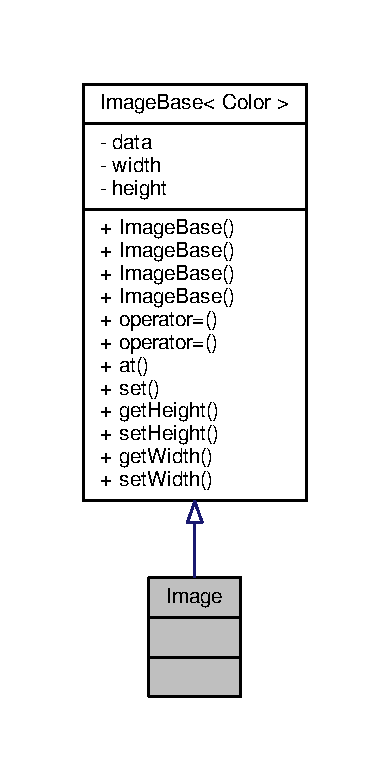
\includegraphics[width=187pt]{d7/da5/class_image__inherit__graph}
\end{center}
\end{figure}


Граф связей класса Image\+:
\nopagebreak
\begin{figure}[H]
\begin{center}
\leavevmode
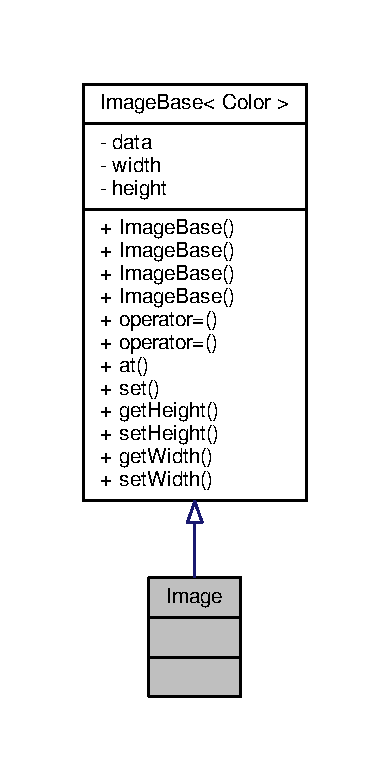
\includegraphics[width=187pt]{d8/d41/class_image__coll__graph}
\end{center}
\end{figure}
\subsection*{Друзья}
\begin{DoxyCompactItemize}
\item 
class \hyperlink{class_image_a683b929065aaead03ccce450a7b4ab30}{Image\+Converter}
\item 
class \hyperlink{class_image_a655e20b76703bb6a4e6ecd9ed4a5d9ed}{Grayscale\+Converter}
\end{DoxyCompactItemize}
\subsection*{Дополнительные унаследованные члены}


\subsection{Подробное описание}


См. определение в файле image.\+h строка 15



\subsection{Документация по друзьям класса и функциям, относящимся к классу}
\index{Image@{Image}!Grayscale\+Converter@{Grayscale\+Converter}}
\index{Grayscale\+Converter@{Grayscale\+Converter}!Image@{Image}}
\subsubsection[{\texorpdfstring{Grayscale\+Converter}{GrayscaleConverter}}]{\setlength{\rightskip}{0pt plus 5cm}friend class Grayscale\+Converter\hspace{0.3cm}{\ttfamily [friend]}}\hypertarget{class_image_a655e20b76703bb6a4e6ecd9ed4a5d9ed}{}\label{class_image_a655e20b76703bb6a4e6ecd9ed4a5d9ed}


См. определение в файле image.\+h строка 21

\index{Image@{Image}!Image\+Converter@{Image\+Converter}}
\index{Image\+Converter@{Image\+Converter}!Image@{Image}}
\subsubsection[{\texorpdfstring{Image\+Converter}{ImageConverter}}]{\setlength{\rightskip}{0pt plus 5cm}friend class {\bf Image\+Converter}\hspace{0.3cm}{\ttfamily [friend]}}\hypertarget{class_image_a683b929065aaead03ccce450a7b4ab30}{}\label{class_image_a683b929065aaead03ccce450a7b4ab30}


См. определение в файле image.\+h строка 20



Объявления и описания членов класса находятся в файле\+:\begin{DoxyCompactItemize}
\item 
Projects/labs/course\+\_\+project\+\_\+cg/src/image/\hyperlink{image_8h}{image.\+h}\end{DoxyCompactItemize}

\hypertarget{class_image_base}{}\section{Шаблон класса Image\+Base$<$ T $>$}
\label{class_image_base}\index{Image\+Base$<$ T $>$@{Image\+Base$<$ T $>$}}


{\ttfamily \#include $<$imagebase.\+h$>$}



Граф связей класса Image\+Base$<$ T $>$\+:
\nopagebreak
\begin{figure}[H]
\begin{center}
\leavevmode
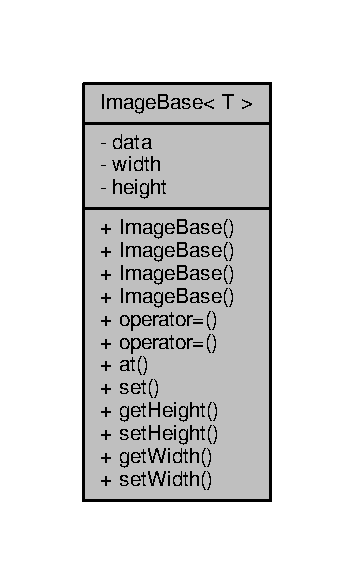
\includegraphics[width=170pt]{d4/d41/class_image_base__coll__graph}
\end{center}
\end{figure}
\subsection*{Открытые члены}
\begin{DoxyCompactItemize}
\item 
\hyperlink{class_image_base_a0d0996266703e4c7bbedf96bc5c6313c}{Image\+Base} ()
\item 
\hyperlink{class_image_base_a43a4b975fe25dfca53ce3f0155dd5976}{Image\+Base} (const \hyperlink{class_image_base}{Image\+Base} \&image)
\item 
\hyperlink{class_image_base_a655bd5b3b40499448b5b204de54de2b2}{Image\+Base} (\hyperlink{class_image_base}{Image\+Base} \&\&image)
\item 
\hyperlink{class_image_base_a6094d4bcf9e48de9b2d66d4f9bbb9db2}{Image\+Base} (\hyperlink{number_8h_a1134b580f8da4de94ca6b1de4d37975e}{uint32} \hyperlink{class_image_base_a2f5f532885f040113c198c424cc0ec7f}{height}, \hyperlink{number_8h_a1134b580f8da4de94ca6b1de4d37975e}{uint32} \hyperlink{class_image_base_a01be4d15909d029bf4ef23f8ed6f6369}{width})
\item 
\hyperlink{class_image_base}{Image\+Base} \& \hyperlink{class_image_base_a84b330cd4e586ff7bed5beee148c3309}{operator=} (const \hyperlink{class_image_base}{Image\+Base} \&image)
\item 
\hyperlink{class_image_base}{Image\+Base} \& \hyperlink{class_image_base_a0def07d97e63c1448751a70e06c3e370}{operator=} (\hyperlink{class_image_base}{Image\+Base} \&\&image)
\item 
const T \& \hyperlink{class_image_base_acf5042cc5679250825272cb23a4594a1}{at} (\hyperlink{number_8h_a1134b580f8da4de94ca6b1de4d37975e}{uint32} i, \hyperlink{number_8h_a1134b580f8da4de94ca6b1de4d37975e}{uint32} j) const 
\item 
void \hyperlink{class_image_base_a2ed65bd7506be1b5bf8ff56a5b56d3a2}{set} (\hyperlink{number_8h_a1134b580f8da4de94ca6b1de4d37975e}{uint32} i, \hyperlink{number_8h_a1134b580f8da4de94ca6b1de4d37975e}{uint32} j, const T \&color)
\item 
\hyperlink{number_8h_a1134b580f8da4de94ca6b1de4d37975e}{uint32} \hyperlink{class_image_base_a750ec0d8ff1dd10dfa26467c018cc68c}{get\+Height} () const 
\item 
void \hyperlink{class_image_base_ac26af0c1bfd19f915f19d6b6f85c05c5}{set\+Height} (\hyperlink{number_8h_a1134b580f8da4de94ca6b1de4d37975e}{uint32} value)
\item 
\hyperlink{number_8h_a1134b580f8da4de94ca6b1de4d37975e}{uint32} \hyperlink{class_image_base_a576197cd4b79d141bb8bd832511fb26a}{get\+Width} () const 
\item 
void \hyperlink{class_image_base_a1448e596fe52852668baa5caefe23f86}{set\+Width} (\hyperlink{number_8h_a1134b580f8da4de94ca6b1de4d37975e}{uint32} value)
\end{DoxyCompactItemize}
\subsection*{Закрытые данные}
\begin{DoxyCompactItemize}
\item 
std\+::unique\+\_\+ptr$<$ T\mbox{[}$\,$\mbox{]}$>$ \hyperlink{class_image_base_aa619aa7a0b2cf0b5e45b0fbc102329c1}{data}
\item 
\hyperlink{number_8h_a1134b580f8da4de94ca6b1de4d37975e}{uint32} \hyperlink{class_image_base_a01be4d15909d029bf4ef23f8ed6f6369}{width}
\item 
\hyperlink{number_8h_a1134b580f8da4de94ca6b1de4d37975e}{uint32} \hyperlink{class_image_base_a2f5f532885f040113c198c424cc0ec7f}{height}
\end{DoxyCompactItemize}
\subsection*{Друзья}
\begin{DoxyCompactItemize}
\item 
class \hyperlink{class_image_base_a683b929065aaead03ccce450a7b4ab30}{Image\+Converter}
\item 
class \hyperlink{class_image_base_a655e20b76703bb6a4e6ecd9ed4a5d9ed}{Grayscale\+Converter}
\end{DoxyCompactItemize}


\subsection{Подробное описание}
\subsubsection*{template$<$class T$>$\\*
class Image\+Base$<$ T $>$}



См. определение в файле imagebase.\+h строка 13



\subsection{Конструктор(ы)}
\index{Image\+Base@{Image\+Base}!Image\+Base@{Image\+Base}}
\index{Image\+Base@{Image\+Base}!Image\+Base@{Image\+Base}}
\subsubsection[{\texorpdfstring{Image\+Base()}{ImageBase()}}]{\setlength{\rightskip}{0pt plus 5cm}template$<$class T $>$ {\bf Image\+Base}$<$ T $>$\+::{\bf Image\+Base} (
\begin{DoxyParamCaption}
{}
\end{DoxyParamCaption}
)}\hypertarget{class_image_base_a0d0996266703e4c7bbedf96bc5c6313c}{}\label{class_image_base_a0d0996266703e4c7bbedf96bc5c6313c}


См. определение в файле imagebase.\+h строка 43

\index{Image\+Base@{Image\+Base}!Image\+Base@{Image\+Base}}
\index{Image\+Base@{Image\+Base}!Image\+Base@{Image\+Base}}
\subsubsection[{\texorpdfstring{Image\+Base(const Image\+Base \&image)}{ImageBase(const ImageBase &image)}}]{\setlength{\rightskip}{0pt plus 5cm}template$<$class T $>$ {\bf Image\+Base}$<$ T $>$\+::{\bf Image\+Base} (
\begin{DoxyParamCaption}
\item[{const {\bf Image\+Base}$<$ T $>$ \&}]{image}
\end{DoxyParamCaption}
)}\hypertarget{class_image_base_a43a4b975fe25dfca53ce3f0155dd5976}{}\label{class_image_base_a43a4b975fe25dfca53ce3f0155dd5976}


См. определение в файле imagebase.\+h строка 51

\index{Image\+Base@{Image\+Base}!Image\+Base@{Image\+Base}}
\index{Image\+Base@{Image\+Base}!Image\+Base@{Image\+Base}}
\subsubsection[{\texorpdfstring{Image\+Base(\+Image\+Base \&\&image)}{ImageBase(ImageBase &&image)}}]{\setlength{\rightskip}{0pt plus 5cm}template$<$class T $>$ {\bf Image\+Base}$<$ T $>$\+::{\bf Image\+Base} (
\begin{DoxyParamCaption}
\item[{{\bf Image\+Base}$<$ T $>$ \&\&}]{image}
\end{DoxyParamCaption}
)}\hypertarget{class_image_base_a655bd5b3b40499448b5b204de54de2b2}{}\label{class_image_base_a655bd5b3b40499448b5b204de54de2b2}


См. определение в файле imagebase.\+h строка 63

\index{Image\+Base@{Image\+Base}!Image\+Base@{Image\+Base}}
\index{Image\+Base@{Image\+Base}!Image\+Base@{Image\+Base}}
\subsubsection[{\texorpdfstring{Image\+Base(uint32 height, uint32 width)}{ImageBase(uint32 height, uint32 width)}}]{\setlength{\rightskip}{0pt plus 5cm}template$<$class T $>$ {\bf Image\+Base}$<$ T $>$\+::{\bf Image\+Base} (
\begin{DoxyParamCaption}
\item[{{\bf uint32}}]{height, }
\item[{{\bf uint32}}]{width}
\end{DoxyParamCaption}
)}\hypertarget{class_image_base_a6094d4bcf9e48de9b2d66d4f9bbb9db2}{}\label{class_image_base_a6094d4bcf9e48de9b2d66d4f9bbb9db2}


См. определение в файле imagebase.\+h строка 72



\subsection{Методы}
\index{Image\+Base@{Image\+Base}!at@{at}}
\index{at@{at}!Image\+Base@{Image\+Base}}
\subsubsection[{\texorpdfstring{at(uint32 i, uint32 j) const }{at(uint32 i, uint32 j) const }}]{\setlength{\rightskip}{0pt plus 5cm}template$<$class T $>$ const T \& {\bf Image\+Base}$<$ T $>$\+::at (
\begin{DoxyParamCaption}
\item[{{\bf uint32}}]{i, }
\item[{{\bf uint32}}]{j}
\end{DoxyParamCaption}
) const}\hypertarget{class_image_base_acf5042cc5679250825272cb23a4594a1}{}\label{class_image_base_acf5042cc5679250825272cb23a4594a1}


См. определение в файле imagebase.\+h строка 111

\index{Image\+Base@{Image\+Base}!get\+Height@{get\+Height}}
\index{get\+Height@{get\+Height}!Image\+Base@{Image\+Base}}
\subsubsection[{\texorpdfstring{get\+Height() const }{getHeight() const }}]{\setlength{\rightskip}{0pt plus 5cm}template$<$class T $>$ {\bf uint32} {\bf Image\+Base}$<$ T $>$\+::get\+Height (
\begin{DoxyParamCaption}
{}
\end{DoxyParamCaption}
) const}\hypertarget{class_image_base_a750ec0d8ff1dd10dfa26467c018cc68c}{}\label{class_image_base_a750ec0d8ff1dd10dfa26467c018cc68c}


См. определение в файле imagebase.\+h строка 123

\index{Image\+Base@{Image\+Base}!get\+Width@{get\+Width}}
\index{get\+Width@{get\+Width}!Image\+Base@{Image\+Base}}
\subsubsection[{\texorpdfstring{get\+Width() const }{getWidth() const }}]{\setlength{\rightskip}{0pt plus 5cm}template$<$class T $>$ {\bf uint32} {\bf Image\+Base}$<$ T $>$\+::get\+Width (
\begin{DoxyParamCaption}
{}
\end{DoxyParamCaption}
) const}\hypertarget{class_image_base_a576197cd4b79d141bb8bd832511fb26a}{}\label{class_image_base_a576197cd4b79d141bb8bd832511fb26a}


См. определение в файле imagebase.\+h строка 135

\index{Image\+Base@{Image\+Base}!operator=@{operator=}}
\index{operator=@{operator=}!Image\+Base@{Image\+Base}}
\subsubsection[{\texorpdfstring{operator=(const Image\+Base \&image)}{operator=(const ImageBase &image)}}]{\setlength{\rightskip}{0pt plus 5cm}template$<$class T $>$ {\bf Image\+Base}$<$ T $>$ \& {\bf Image\+Base}$<$ T $>$\+::operator= (
\begin{DoxyParamCaption}
\item[{const {\bf Image\+Base}$<$ T $>$ \&}]{image}
\end{DoxyParamCaption}
)}\hypertarget{class_image_base_a84b330cd4e586ff7bed5beee148c3309}{}\label{class_image_base_a84b330cd4e586ff7bed5beee148c3309}


См. определение в файле imagebase.\+h строка 85

\index{Image\+Base@{Image\+Base}!operator=@{operator=}}
\index{operator=@{operator=}!Image\+Base@{Image\+Base}}
\subsubsection[{\texorpdfstring{operator=(\+Image\+Base \&\&image)}{operator=(ImageBase &&image)}}]{\setlength{\rightskip}{0pt plus 5cm}template$<$class T $>$ {\bf Image\+Base}$<$ T $>$ \& {\bf Image\+Base}$<$ T $>$\+::operator= (
\begin{DoxyParamCaption}
\item[{{\bf Image\+Base}$<$ T $>$ \&\&}]{image}
\end{DoxyParamCaption}
)}\hypertarget{class_image_base_a0def07d97e63c1448751a70e06c3e370}{}\label{class_image_base_a0def07d97e63c1448751a70e06c3e370}


См. определение в файле imagebase.\+h строка 100

\index{Image\+Base@{Image\+Base}!set@{set}}
\index{set@{set}!Image\+Base@{Image\+Base}}
\subsubsection[{\texorpdfstring{set(uint32 i, uint32 j, const T \&color)}{set(uint32 i, uint32 j, const T &color)}}]{\setlength{\rightskip}{0pt plus 5cm}template$<$class T$>$ void {\bf Image\+Base}$<$ T $>$\+::set (
\begin{DoxyParamCaption}
\item[{{\bf uint32}}]{i, }
\item[{{\bf uint32}}]{j, }
\item[{const T \&}]{color}
\end{DoxyParamCaption}
)}\hypertarget{class_image_base_a2ed65bd7506be1b5bf8ff56a5b56d3a2}{}\label{class_image_base_a2ed65bd7506be1b5bf8ff56a5b56d3a2}


См. определение в файле imagebase.\+h строка 117

\index{Image\+Base@{Image\+Base}!set\+Height@{set\+Height}}
\index{set\+Height@{set\+Height}!Image\+Base@{Image\+Base}}
\subsubsection[{\texorpdfstring{set\+Height(uint32 value)}{setHeight(uint32 value)}}]{\setlength{\rightskip}{0pt plus 5cm}template$<$class T $>$ void {\bf Image\+Base}$<$ T $>$\+::set\+Height (
\begin{DoxyParamCaption}
\item[{{\bf uint32}}]{value}
\end{DoxyParamCaption}
)}\hypertarget{class_image_base_ac26af0c1bfd19f915f19d6b6f85c05c5}{}\label{class_image_base_ac26af0c1bfd19f915f19d6b6f85c05c5}


См. определение в файле imagebase.\+h строка 129

\index{Image\+Base@{Image\+Base}!set\+Width@{set\+Width}}
\index{set\+Width@{set\+Width}!Image\+Base@{Image\+Base}}
\subsubsection[{\texorpdfstring{set\+Width(uint32 value)}{setWidth(uint32 value)}}]{\setlength{\rightskip}{0pt plus 5cm}template$<$class T $>$ void {\bf Image\+Base}$<$ T $>$\+::set\+Width (
\begin{DoxyParamCaption}
\item[{{\bf uint32}}]{value}
\end{DoxyParamCaption}
)}\hypertarget{class_image_base_a1448e596fe52852668baa5caefe23f86}{}\label{class_image_base_a1448e596fe52852668baa5caefe23f86}


См. определение в файле imagebase.\+h строка 141



\subsection{Документация по друзьям класса и функциям, относящимся к классу}
\index{Image\+Base@{Image\+Base}!Grayscale\+Converter@{Grayscale\+Converter}}
\index{Grayscale\+Converter@{Grayscale\+Converter}!Image\+Base@{Image\+Base}}
\subsubsection[{\texorpdfstring{Grayscale\+Converter}{GrayscaleConverter}}]{\setlength{\rightskip}{0pt plus 5cm}template$<$class T$>$ friend class Grayscale\+Converter\hspace{0.3cm}{\ttfamily [friend]}}\hypertarget{class_image_base_a655e20b76703bb6a4e6ecd9ed4a5d9ed}{}\label{class_image_base_a655e20b76703bb6a4e6ecd9ed4a5d9ed}


См. определение в файле imagebase.\+h строка 39

\index{Image\+Base@{Image\+Base}!Image\+Converter@{Image\+Converter}}
\index{Image\+Converter@{Image\+Converter}!Image\+Base@{Image\+Base}}
\subsubsection[{\texorpdfstring{Image\+Converter}{ImageConverter}}]{\setlength{\rightskip}{0pt plus 5cm}template$<$class T$>$ friend class {\bf Image\+Converter}\hspace{0.3cm}{\ttfamily [friend]}}\hypertarget{class_image_base_a683b929065aaead03ccce450a7b4ab30}{}\label{class_image_base_a683b929065aaead03ccce450a7b4ab30}


См. определение в файле imagebase.\+h строка 38



\subsection{Данные класса}
\index{Image\+Base@{Image\+Base}!data@{data}}
\index{data@{data}!Image\+Base@{Image\+Base}}
\subsubsection[{\texorpdfstring{data}{data}}]{\setlength{\rightskip}{0pt plus 5cm}template$<$class T$>$ std\+::unique\+\_\+ptr$<$T\mbox{[}$\,$\mbox{]}$>$ {\bf Image\+Base}$<$ T $>$\+::data\hspace{0.3cm}{\ttfamily [private]}}\hypertarget{class_image_base_aa619aa7a0b2cf0b5e45b0fbc102329c1}{}\label{class_image_base_aa619aa7a0b2cf0b5e45b0fbc102329c1}


См. определение в файле imagebase.\+h строка 35

\index{Image\+Base@{Image\+Base}!height@{height}}
\index{height@{height}!Image\+Base@{Image\+Base}}
\subsubsection[{\texorpdfstring{height}{height}}]{\setlength{\rightskip}{0pt plus 5cm}template$<$class T$>$ {\bf uint32} {\bf Image\+Base}$<$ T $>$\+::height\hspace{0.3cm}{\ttfamily [private]}}\hypertarget{class_image_base_a2f5f532885f040113c198c424cc0ec7f}{}\label{class_image_base_a2f5f532885f040113c198c424cc0ec7f}


См. определение в файле imagebase.\+h строка 36

\index{Image\+Base@{Image\+Base}!width@{width}}
\index{width@{width}!Image\+Base@{Image\+Base}}
\subsubsection[{\texorpdfstring{width}{width}}]{\setlength{\rightskip}{0pt plus 5cm}template$<$class T$>$ {\bf uint32} {\bf Image\+Base}$<$ T $>$\+::width\hspace{0.3cm}{\ttfamily [private]}}\hypertarget{class_image_base_a01be4d15909d029bf4ef23f8ed6f6369}{}\label{class_image_base_a01be4d15909d029bf4ef23f8ed6f6369}


См. определение в файле imagebase.\+h строка 36



Объявления и описания членов класса находятся в файле\+:\begin{DoxyCompactItemize}
\item 
Projects/labs/course\+\_\+project\+\_\+cg/src/image/\hyperlink{imagebase_8h}{imagebase.\+h}\end{DoxyCompactItemize}

\hypertarget{class_image_converter}{}\section{Класс Image\+Converter}
\label{class_image_converter}\index{Image\+Converter@{Image\+Converter}}


{\ttfamily \#include $<$imageconverter.\+h$>$}



Граф связей класса Image\+Converter\+:
\nopagebreak
\begin{figure}[H]
\begin{center}
\leavevmode
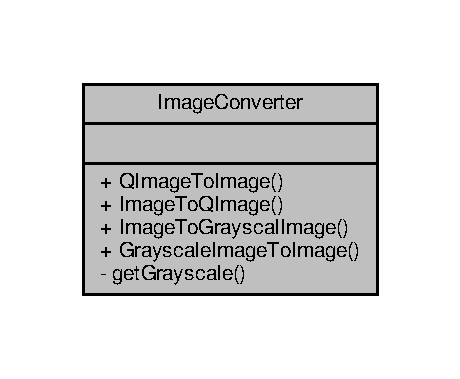
\includegraphics[width=221pt]{d1/da6/class_image_converter__coll__graph}
\end{center}
\end{figure}
\subsection*{Открытые статические члены}
\begin{DoxyCompactItemize}
\item 
static \hyperlink{class_image}{Image} \hyperlink{class_image_converter_a5c0f28c5f9da5f2c64077e8dc7462a03}{Q\+Image\+To\+Image} (const Q\+Image \&q\+Image)
\item 
static Q\+Image \hyperlink{class_image_converter_a1d4ec9d93d250b7db9dc8fbf28c513cf}{Image\+To\+Q\+Image} (const \hyperlink{class_image}{Image} \&image)
\item 
static \hyperlink{class_grayscale_image}{Grayscale\+Image} \hyperlink{class_image_converter_a58b9e3e65e60d89986327f90bf305069}{Image\+To\+Grayscal\+Image} (const \hyperlink{class_image}{Image} \&image)
\item 
static \hyperlink{class_image}{Image} \hyperlink{class_image_converter_a43b58fb52b437bad20fb9dbb57f01067}{Grayscale\+Image\+To\+Image} (const \hyperlink{class_grayscale_image}{Grayscale\+Image} \&image)
\end{DoxyCompactItemize}
\subsection*{Закрытые статические члены}
\begin{DoxyCompactItemize}
\item 
static \hyperlink{number_8h_adde6aaee8457bee49c2a92621fe22b79}{uint8} \hyperlink{class_image_converter_a478c9d613c0591f3a0f0f0db6081b986}{get\+Grayscale} (const \hyperlink{class_color}{Color} \&color)
\end{DoxyCompactItemize}


\subsection{Подробное описание}


См. определение в файле imageconverter.\+h строка 9



\subsection{Методы}
\index{Image\+Converter@{Image\+Converter}!get\+Grayscale@{get\+Grayscale}}
\index{get\+Grayscale@{get\+Grayscale}!Image\+Converter@{Image\+Converter}}
\subsubsection[{\texorpdfstring{get\+Grayscale(const Color \&color)}{getGrayscale(const Color &color)}}]{\setlength{\rightskip}{0pt plus 5cm}{\bf uint8} Image\+Converter\+::get\+Grayscale (
\begin{DoxyParamCaption}
\item[{const {\bf Color} \&}]{color}
\end{DoxyParamCaption}
)\hspace{0.3cm}{\ttfamily [static]}, {\ttfamily [private]}}\hypertarget{class_image_converter_a478c9d613c0591f3a0f0f0db6081b986}{}\label{class_image_converter_a478c9d613c0591f3a0f0f0db6081b986}


См. определение в файле imageconverter.\+cpp строка 53

\index{Image\+Converter@{Image\+Converter}!Grayscale\+Image\+To\+Image@{Grayscale\+Image\+To\+Image}}
\index{Grayscale\+Image\+To\+Image@{Grayscale\+Image\+To\+Image}!Image\+Converter@{Image\+Converter}}
\subsubsection[{\texorpdfstring{Grayscale\+Image\+To\+Image(const Grayscale\+Image \&image)}{GrayscaleImageToImage(const GrayscaleImage &image)}}]{\setlength{\rightskip}{0pt plus 5cm}{\bf Image} Image\+Converter\+::\+Grayscale\+Image\+To\+Image (
\begin{DoxyParamCaption}
\item[{const {\bf Grayscale\+Image} \&}]{image}
\end{DoxyParamCaption}
)\hspace{0.3cm}{\ttfamily [static]}}\hypertarget{class_image_converter_a43b58fb52b437bad20fb9dbb57f01067}{}\label{class_image_converter_a43b58fb52b437bad20fb9dbb57f01067}


См. определение в файле imageconverter.\+cpp строка 61

\index{Image\+Converter@{Image\+Converter}!Image\+To\+Grayscal\+Image@{Image\+To\+Grayscal\+Image}}
\index{Image\+To\+Grayscal\+Image@{Image\+To\+Grayscal\+Image}!Image\+Converter@{Image\+Converter}}
\subsubsection[{\texorpdfstring{Image\+To\+Grayscal\+Image(const Image \&image)}{ImageToGrayscalImage(const Image &image)}}]{\setlength{\rightskip}{0pt plus 5cm}{\bf Grayscale\+Image} Image\+Converter\+::\+Image\+To\+Grayscal\+Image (
\begin{DoxyParamCaption}
\item[{const {\bf Image} \&}]{image}
\end{DoxyParamCaption}
)\hspace{0.3cm}{\ttfamily [static]}}\hypertarget{class_image_converter_a58b9e3e65e60d89986327f90bf305069}{}\label{class_image_converter_a58b9e3e65e60d89986327f90bf305069}


См. определение в файле imageconverter.\+cpp строка 41

\index{Image\+Converter@{Image\+Converter}!Image\+To\+Q\+Image@{Image\+To\+Q\+Image}}
\index{Image\+To\+Q\+Image@{Image\+To\+Q\+Image}!Image\+Converter@{Image\+Converter}}
\subsubsection[{\texorpdfstring{Image\+To\+Q\+Image(const Image \&image)}{ImageToQImage(const Image &image)}}]{\setlength{\rightskip}{0pt plus 5cm}Q\+Image Image\+Converter\+::\+Image\+To\+Q\+Image (
\begin{DoxyParamCaption}
\item[{const {\bf Image} \&}]{image}
\end{DoxyParamCaption}
)\hspace{0.3cm}{\ttfamily [static]}}\hypertarget{class_image_converter_a1d4ec9d93d250b7db9dc8fbf28c513cf}{}\label{class_image_converter_a1d4ec9d93d250b7db9dc8fbf28c513cf}


См. определение в файле imageconverter.\+cpp строка 24

\index{Image\+Converter@{Image\+Converter}!Q\+Image\+To\+Image@{Q\+Image\+To\+Image}}
\index{Q\+Image\+To\+Image@{Q\+Image\+To\+Image}!Image\+Converter@{Image\+Converter}}
\subsubsection[{\texorpdfstring{Q\+Image\+To\+Image(const Q\+Image \&q\+Image)}{QImageToImage(const QImage &qImage)}}]{\setlength{\rightskip}{0pt plus 5cm}{\bf Image} Image\+Converter\+::\+Q\+Image\+To\+Image (
\begin{DoxyParamCaption}
\item[{const Q\+Image \&}]{q\+Image}
\end{DoxyParamCaption}
)\hspace{0.3cm}{\ttfamily [static]}}\hypertarget{class_image_converter_a5c0f28c5f9da5f2c64077e8dc7462a03}{}\label{class_image_converter_a5c0f28c5f9da5f2c64077e8dc7462a03}


См. определение в файле imageconverter.\+cpp строка 4



Объявления и описания членов классов находятся в файлах\+:\begin{DoxyCompactItemize}
\item 
Projects/labs/course\+\_\+project\+\_\+cg/src/image/\hyperlink{imageconverter_8h}{imageconverter.\+h}\item 
Projects/labs/course\+\_\+project\+\_\+cg/src/image/\hyperlink{imageconverter_8cpp}{imageconverter.\+cpp}\end{DoxyCompactItemize}

\hypertarget{class_image_view}{}\section{Класс Image\+View}
\label{class_image_view}\index{Image\+View@{Image\+View}}


{\ttfamily \#include $<$imageview.\+h$>$}



Граф наследования\+:Image\+View\+:
\nopagebreak
\begin{figure}[H]
\begin{center}
\leavevmode
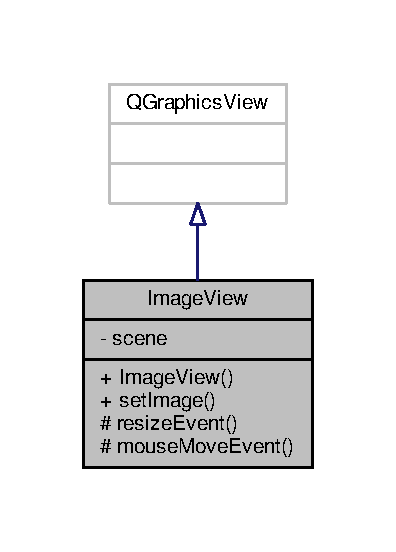
\includegraphics[width=190pt]{df/dd0/class_image_view__inherit__graph}
\end{center}
\end{figure}


Граф связей класса Image\+View\+:
\nopagebreak
\begin{figure}[H]
\begin{center}
\leavevmode
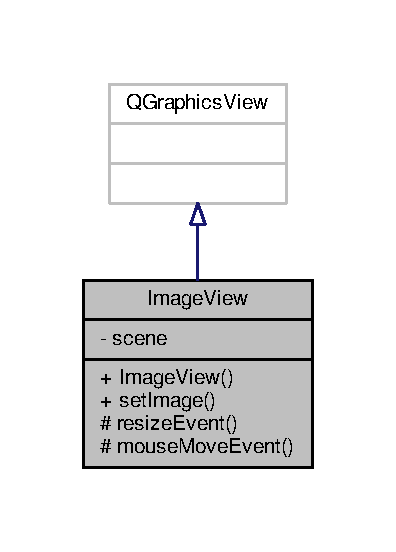
\includegraphics[width=190pt]{d5/d39/class_image_view__coll__graph}
\end{center}
\end{figure}
\subsection*{Открытые члены}
\begin{DoxyCompactItemize}
\item 
\hyperlink{class_image_view_ab9dfd4d7ac8503631906b1c35ad2d445}{Image\+View} (Q\+Widget $\ast$parent=0)
\item 
void \hyperlink{class_image_view_a450337ded2ce7bb5444b6f249e68d13d}{set\+Image} (const Q\+Image \&image)
\end{DoxyCompactItemize}
\subsection*{Защищенные члены}
\begin{DoxyCompactItemize}
\item 
void \hyperlink{class_image_view_a0bcc3711738a814ce221127d0b7ecf5b}{resize\+Event} (Q\+Resize\+Event $\ast$event)
\item 
void \hyperlink{class_image_view_a29a6e4346d585008cf72be75d06e7daa}{mouse\+Move\+Event} (Q\+Mouse\+Event $\ast$)
\end{DoxyCompactItemize}
\subsection*{Закрытые данные}
\begin{DoxyCompactItemize}
\item 
Q\+Graphics\+Scene $\ast$ \hyperlink{class_image_view_a371e669523a21ae10284613a0d84ff6b}{scene}
\end{DoxyCompactItemize}


\subsection{Подробное описание}


См. определение в файле imageview.\+h строка 11



\subsection{Конструктор(ы)}
\index{Image\+View@{Image\+View}!Image\+View@{Image\+View}}
\index{Image\+View@{Image\+View}!Image\+View@{Image\+View}}
\subsubsection[{\texorpdfstring{Image\+View(\+Q\+Widget $\ast$parent=0)}{ImageView(QWidget *parent=0)}}]{\setlength{\rightskip}{0pt plus 5cm}Image\+View\+::\+Image\+View (
\begin{DoxyParamCaption}
\item[{Q\+Widget $\ast$}]{parent = {\ttfamily 0}}
\end{DoxyParamCaption}
)\hspace{0.3cm}{\ttfamily [explicit]}}\hypertarget{class_image_view_ab9dfd4d7ac8503631906b1c35ad2d445}{}\label{class_image_view_ab9dfd4d7ac8503631906b1c35ad2d445}


См. определение в файле imageview.\+cpp строка 5



\subsection{Методы}
\index{Image\+View@{Image\+View}!mouse\+Move\+Event@{mouse\+Move\+Event}}
\index{mouse\+Move\+Event@{mouse\+Move\+Event}!Image\+View@{Image\+View}}
\subsubsection[{\texorpdfstring{mouse\+Move\+Event(\+Q\+Mouse\+Event $\ast$)}{mouseMoveEvent(QMouseEvent *)}}]{\setlength{\rightskip}{0pt plus 5cm}void Image\+View\+::mouse\+Move\+Event (
\begin{DoxyParamCaption}
\item[{Q\+Mouse\+Event $\ast$}]{}
\end{DoxyParamCaption}
)\hspace{0.3cm}{\ttfamily [protected]}}\hypertarget{class_image_view_a29a6e4346d585008cf72be75d06e7daa}{}\label{class_image_view_a29a6e4346d585008cf72be75d06e7daa}


См. определение в файле imageview.\+cpp строка 28

\index{Image\+View@{Image\+View}!resize\+Event@{resize\+Event}}
\index{resize\+Event@{resize\+Event}!Image\+View@{Image\+View}}
\subsubsection[{\texorpdfstring{resize\+Event(\+Q\+Resize\+Event $\ast$event)}{resizeEvent(QResizeEvent *event)}}]{\setlength{\rightskip}{0pt plus 5cm}void Image\+View\+::resize\+Event (
\begin{DoxyParamCaption}
\item[{Q\+Resize\+Event $\ast$}]{event}
\end{DoxyParamCaption}
)\hspace{0.3cm}{\ttfamily [protected]}}\hypertarget{class_image_view_a0bcc3711738a814ce221127d0b7ecf5b}{}\label{class_image_view_a0bcc3711738a814ce221127d0b7ecf5b}


См. определение в файле imageview.\+cpp строка 22

\index{Image\+View@{Image\+View}!set\+Image@{set\+Image}}
\index{set\+Image@{set\+Image}!Image\+View@{Image\+View}}
\subsubsection[{\texorpdfstring{set\+Image(const Q\+Image \&image)}{setImage(const QImage &image)}}]{\setlength{\rightskip}{0pt plus 5cm}void Image\+View\+::set\+Image (
\begin{DoxyParamCaption}
\item[{const Q\+Image \&}]{image}
\end{DoxyParamCaption}
)}\hypertarget{class_image_view_a450337ded2ce7bb5444b6f249e68d13d}{}\label{class_image_view_a450337ded2ce7bb5444b6f249e68d13d}


См. определение в файле imageview.\+cpp строка 15



\subsection{Данные класса}
\index{Image\+View@{Image\+View}!scene@{scene}}
\index{scene@{scene}!Image\+View@{Image\+View}}
\subsubsection[{\texorpdfstring{scene}{scene}}]{\setlength{\rightskip}{0pt plus 5cm}Q\+Graphics\+Scene$\ast$ Image\+View\+::scene\hspace{0.3cm}{\ttfamily [private]}}\hypertarget{class_image_view_a371e669523a21ae10284613a0d84ff6b}{}\label{class_image_view_a371e669523a21ae10284613a0d84ff6b}


См. определение в файле imageview.\+h строка 24



Объявления и описания членов классов находятся в файлах\+:\begin{DoxyCompactItemize}
\item 
Projects/labs/course\+\_\+project\+\_\+cg/src/widgets/\hyperlink{imageview_8h}{imageview.\+h}\item 
Projects/labs/course\+\_\+project\+\_\+cg/src/widgets/\hyperlink{imageview_8cpp}{imageview.\+cpp}\end{DoxyCompactItemize}

\hypertarget{class_light}{}\section{Класс Light}
\label{class_light}\index{Light@{Light}}


{\ttfamily \#include $<$light.\+h$>$}



Граф наследования\+:Light\+:
\nopagebreak
\begin{figure}[H]
\begin{center}
\leavevmode
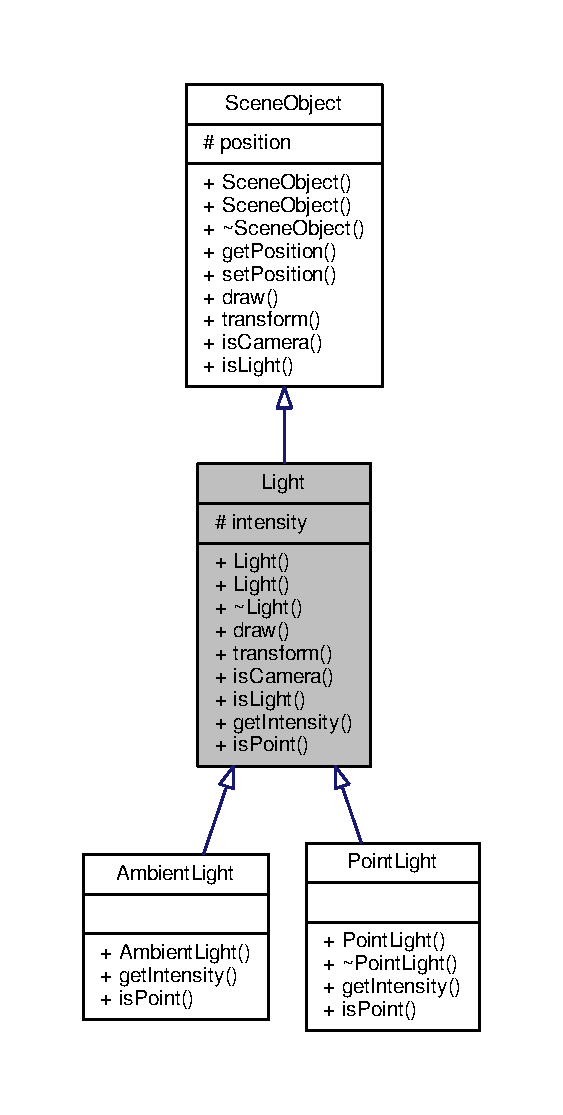
\includegraphics[width=270pt]{dd/d00/class_light__inherit__graph}
\end{center}
\end{figure}


Граф связей класса Light\+:
\nopagebreak
\begin{figure}[H]
\begin{center}
\leavevmode
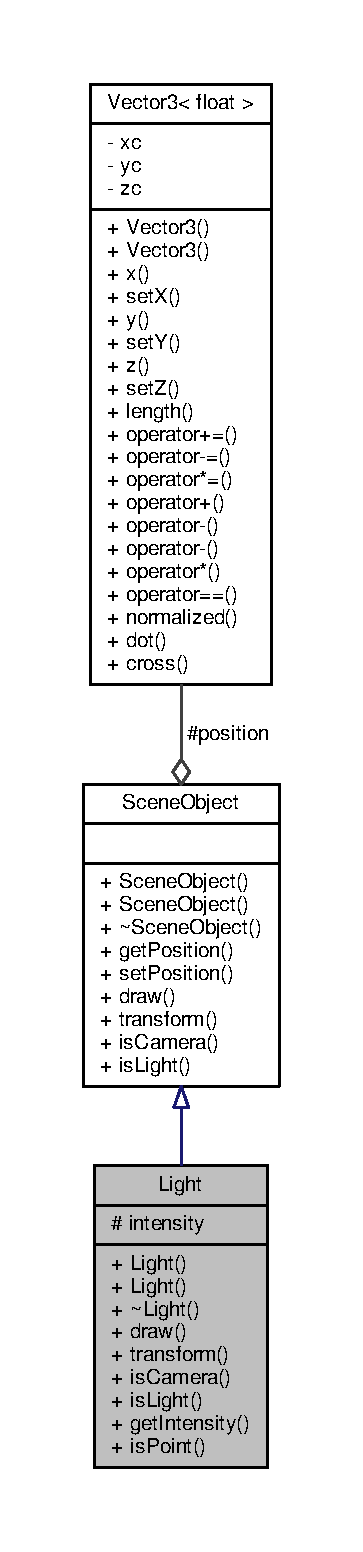
\includegraphics[height=550pt]{df/d88/class_light__coll__graph}
\end{center}
\end{figure}
\subsection*{Открытые члены}
\begin{DoxyCompactItemize}
\item 
\hyperlink{class_light_af49ca6a5dd2fb43fb878a5ad5f0409fe}{Light} ()=default
\item 
\hyperlink{class_light_adc14c27a60cc0b1d86fdc2f44858c705}{Light} (const \hyperlink{vec3_8h_a221ad8ea4d9be4111628ee1ca22ee3ba}{Vec3} \&\hyperlink{class_scene_object_af190cdf9b9449f96f73d836848ce4ad3}{position}, float \hyperlink{class_light_a1071eaa556f4bb2a9345fdfba7e6f220}{intensity})
\item 
virtual \hyperlink{class_light_ae3e3209d4b97d0bbbd614ded5e1213d9}{$\sim$\+Light} ()=default
\item 
virtual void \hyperlink{class_light_a5ae4db3ece8e61f53db06e8d3af4cdca}{draw} (std\+::unique\+\_\+ptr$<$ \hyperlink{class_renderer}{Renderer} $>$ \&) override
\item 
virtual void \hyperlink{class_light_afb03030e1dd8056c73e813095701d796}{transform} (\hyperlink{class_transformation}{Transformation} \&transformation) override
\item 
virtual bool \hyperlink{class_light_a942b4fb690c63be248ae031723a6148c}{is\+Camera} () override
\item 
virtual bool \hyperlink{class_light_af09370083a781d2733247bc2ee2f4c33}{is\+Light} () override
\item 
virtual \hyperlink{class_color}{Color} \hyperlink{class_light_a81a8d20cdba6692644cda765aced1473}{get\+Intensity} (const \hyperlink{vec3_8h_a221ad8ea4d9be4111628ee1ca22ee3ba}{Vec3} \&normal, const \hyperlink{vec3_8h_a221ad8ea4d9be4111628ee1ca22ee3ba}{Vec3} \&\hyperlink{class_scene_object_af190cdf9b9449f96f73d836848ce4ad3}{position}, const \hyperlink{vec3_8h_a221ad8ea4d9be4111628ee1ca22ee3ba}{Vec3} \&camera, const \hyperlink{class_color}{Color} \&ka, const \hyperlink{class_color}{Color} \&kd, const \hyperlink{class_color}{Color} \&ks, float ns) const =0
\item 
virtual bool \hyperlink{class_light_aa17c9733d1616d8631ed63640344b733}{is\+Point} () const =0
\end{DoxyCompactItemize}
\subsection*{Защищенные данные}
\begin{DoxyCompactItemize}
\item 
float \hyperlink{class_light_a1071eaa556f4bb2a9345fdfba7e6f220}{intensity}
\end{DoxyCompactItemize}


\subsection{Подробное описание}


См. определение в файле light.\+h строка 7



\subsection{Конструктор(ы)}
\index{Light@{Light}!Light@{Light}}
\index{Light@{Light}!Light@{Light}}
\subsubsection[{\texorpdfstring{Light()=default}{Light()=default}}]{\setlength{\rightskip}{0pt plus 5cm}Light\+::\+Light (
\begin{DoxyParamCaption}
{}
\end{DoxyParamCaption}
)\hspace{0.3cm}{\ttfamily [default]}}\hypertarget{class_light_af49ca6a5dd2fb43fb878a5ad5f0409fe}{}\label{class_light_af49ca6a5dd2fb43fb878a5ad5f0409fe}
\index{Light@{Light}!Light@{Light}}
\index{Light@{Light}!Light@{Light}}
\subsubsection[{\texorpdfstring{Light(const Vec3 \&position, float intensity)}{Light(const Vec3 &position, float intensity)}}]{\setlength{\rightskip}{0pt plus 5cm}Light\+::\+Light (
\begin{DoxyParamCaption}
\item[{const {\bf Vec3} \&}]{position, }
\item[{float}]{intensity}
\end{DoxyParamCaption}
)}\hypertarget{class_light_adc14c27a60cc0b1d86fdc2f44858c705}{}\label{class_light_adc14c27a60cc0b1d86fdc2f44858c705}


См. определение в файле light.\+cpp строка 4

\index{Light@{Light}!````~Light@{$\sim$\+Light}}
\index{````~Light@{$\sim$\+Light}!Light@{Light}}
\subsubsection[{\texorpdfstring{$\sim$\+Light()=default}{~Light()=default}}]{\setlength{\rightskip}{0pt plus 5cm}virtual Light\+::$\sim$\+Light (
\begin{DoxyParamCaption}
{}
\end{DoxyParamCaption}
)\hspace{0.3cm}{\ttfamily [virtual]}, {\ttfamily [default]}}\hypertarget{class_light_ae3e3209d4b97d0bbbd614ded5e1213d9}{}\label{class_light_ae3e3209d4b97d0bbbd614ded5e1213d9}


\subsection{Методы}
\index{Light@{Light}!draw@{draw}}
\index{draw@{draw}!Light@{Light}}
\subsubsection[{\texorpdfstring{draw(std\+::unique\+\_\+ptr$<$ Renderer $>$ \&) override}{draw(std::unique_ptr< Renderer > &) override}}]{\setlength{\rightskip}{0pt plus 5cm}void Light\+::draw (
\begin{DoxyParamCaption}
\item[{std\+::unique\+\_\+ptr$<$ {\bf Renderer} $>$ \&}]{}
\end{DoxyParamCaption}
)\hspace{0.3cm}{\ttfamily [override]}, {\ttfamily [virtual]}}\hypertarget{class_light_a5ae4db3ece8e61f53db06e8d3af4cdca}{}\label{class_light_a5ae4db3ece8e61f53db06e8d3af4cdca}


Замещает \hyperlink{class_scene_object_adc906ce4e4a896a351949ccabfd44016}{Scene\+Object}.



См. определение в файле light.\+cpp строка 10

\index{Light@{Light}!get\+Intensity@{get\+Intensity}}
\index{get\+Intensity@{get\+Intensity}!Light@{Light}}
\subsubsection[{\texorpdfstring{get\+Intensity(const Vec3 \&normal, const Vec3 \&position, const Vec3 \&camera, const Color \&ka, const Color \&kd, const Color \&ks, float ns) const =0}{getIntensity(const Vec3 &normal, const Vec3 &position, const Vec3 &camera, const Color &ka, const Color &kd, const Color &ks, float ns) const =0}}]{\setlength{\rightskip}{0pt plus 5cm}virtual {\bf Color} Light\+::get\+Intensity (
\begin{DoxyParamCaption}
\item[{const {\bf Vec3} \&}]{normal, }
\item[{const {\bf Vec3} \&}]{position, }
\item[{const {\bf Vec3} \&}]{camera, }
\item[{const {\bf Color} \&}]{ka, }
\item[{const {\bf Color} \&}]{kd, }
\item[{const {\bf Color} \&}]{ks, }
\item[{float}]{ns}
\end{DoxyParamCaption}
) const\hspace{0.3cm}{\ttfamily [pure virtual]}}\hypertarget{class_light_a81a8d20cdba6692644cda765aced1473}{}\label{class_light_a81a8d20cdba6692644cda765aced1473}


Замещается в \hyperlink{class_point_light_a1fc0406a41b9474e7568bf925287fabe}{Point\+Light} и \hyperlink{class_ambient_light_aebbccf2534a3cbe399ccddc552d1a49d}{Ambient\+Light}.

\index{Light@{Light}!is\+Camera@{is\+Camera}}
\index{is\+Camera@{is\+Camera}!Light@{Light}}
\subsubsection[{\texorpdfstring{is\+Camera() override}{isCamera() override}}]{\setlength{\rightskip}{0pt plus 5cm}bool Light\+::is\+Camera (
\begin{DoxyParamCaption}
{}
\end{DoxyParamCaption}
)\hspace{0.3cm}{\ttfamily [override]}, {\ttfamily [virtual]}}\hypertarget{class_light_a942b4fb690c63be248ae031723a6148c}{}\label{class_light_a942b4fb690c63be248ae031723a6148c}


Замещает \hyperlink{class_scene_object_a6d7cb8b9a2c29f38fd039731e83167f4}{Scene\+Object}.



См. определение в файле light.\+cpp строка 19

\index{Light@{Light}!is\+Light@{is\+Light}}
\index{is\+Light@{is\+Light}!Light@{Light}}
\subsubsection[{\texorpdfstring{is\+Light() override}{isLight() override}}]{\setlength{\rightskip}{0pt plus 5cm}bool Light\+::is\+Light (
\begin{DoxyParamCaption}
{}
\end{DoxyParamCaption}
)\hspace{0.3cm}{\ttfamily [override]}, {\ttfamily [virtual]}}\hypertarget{class_light_af09370083a781d2733247bc2ee2f4c33}{}\label{class_light_af09370083a781d2733247bc2ee2f4c33}


Замещает \hyperlink{class_scene_object_a9c5b006b8a0e457634f15c19eb51ca73}{Scene\+Object}.



См. определение в файле light.\+cpp строка 24

\index{Light@{Light}!is\+Point@{is\+Point}}
\index{is\+Point@{is\+Point}!Light@{Light}}
\subsubsection[{\texorpdfstring{is\+Point() const =0}{isPoint() const =0}}]{\setlength{\rightskip}{0pt plus 5cm}virtual bool Light\+::is\+Point (
\begin{DoxyParamCaption}
{}
\end{DoxyParamCaption}
) const\hspace{0.3cm}{\ttfamily [pure virtual]}}\hypertarget{class_light_aa17c9733d1616d8631ed63640344b733}{}\label{class_light_aa17c9733d1616d8631ed63640344b733}


Замещается в \hyperlink{class_point_light_a002882a80254c1b99bd45f5a97f25e99}{Point\+Light} и \hyperlink{class_ambient_light_accccb9b3c5f0a9c38dceaef386c2964a}{Ambient\+Light}.

\index{Light@{Light}!transform@{transform}}
\index{transform@{transform}!Light@{Light}}
\subsubsection[{\texorpdfstring{transform(\+Transformation \&transformation) override}{transform(Transformation &transformation) override}}]{\setlength{\rightskip}{0pt plus 5cm}void Light\+::transform (
\begin{DoxyParamCaption}
\item[{{\bf Transformation} \&}]{transformation}
\end{DoxyParamCaption}
)\hspace{0.3cm}{\ttfamily [override]}, {\ttfamily [virtual]}}\hypertarget{class_light_afb03030e1dd8056c73e813095701d796}{}\label{class_light_afb03030e1dd8056c73e813095701d796}


Замещает \hyperlink{class_scene_object_a1b8a4b90f1200f1cd025d95964d43630}{Scene\+Object}.



См. определение в файле light.\+cpp строка 14



\subsection{Данные класса}
\index{Light@{Light}!intensity@{intensity}}
\index{intensity@{intensity}!Light@{Light}}
\subsubsection[{\texorpdfstring{intensity}{intensity}}]{\setlength{\rightskip}{0pt plus 5cm}float Light\+::intensity\hspace{0.3cm}{\ttfamily [protected]}}\hypertarget{class_light_a1071eaa556f4bb2a9345fdfba7e6f220}{}\label{class_light_a1071eaa556f4bb2a9345fdfba7e6f220}


См. определение в файле light.\+h строка 26



Объявления и описания членов классов находятся в файлах\+:\begin{DoxyCompactItemize}
\item 
Projects/labs/course\+\_\+project\+\_\+cg/src/animation/\hyperlink{light_8h}{light.\+h}\item 
Projects/labs/course\+\_\+project\+\_\+cg/src/animation/\hyperlink{light_8cpp}{light.\+cpp}\end{DoxyCompactItemize}

\hypertarget{class_light_z_buffer_renderer}{}\section{Класс Light\+Z\+Buffer\+Renderer}
\label{class_light_z_buffer_renderer}\index{Light\+Z\+Buffer\+Renderer@{Light\+Z\+Buffer\+Renderer}}


{\ttfamily \#include $<$lightzbufferrenderer.\+h$>$}



Граф наследования\+:Light\+Z\+Buffer\+Renderer\+:
\nopagebreak
\begin{figure}[H]
\begin{center}
\leavevmode
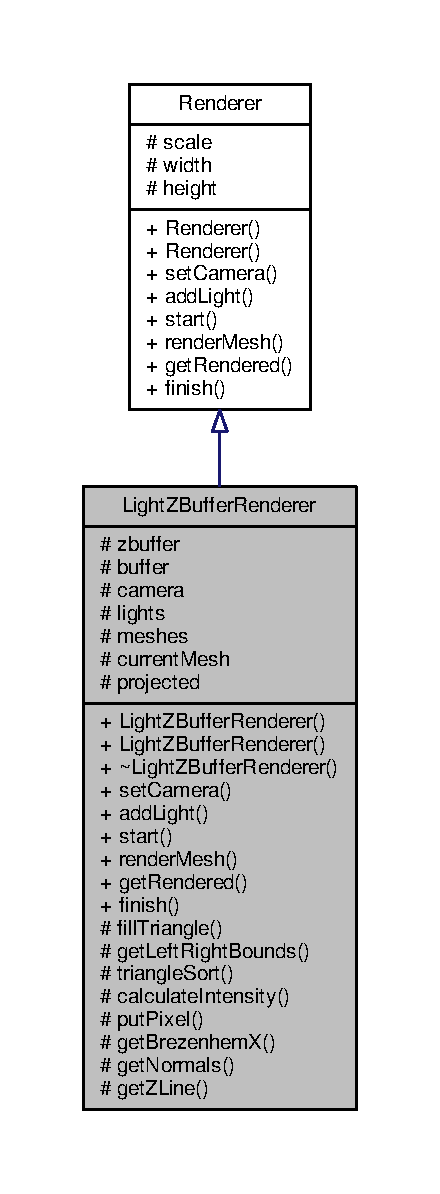
\includegraphics[height=550pt]{db/dd8/class_light_z_buffer_renderer__inherit__graph}
\end{center}
\end{figure}


Граф связей класса Light\+Z\+Buffer\+Renderer\+:
\nopagebreak
\begin{figure}[H]
\begin{center}
\leavevmode
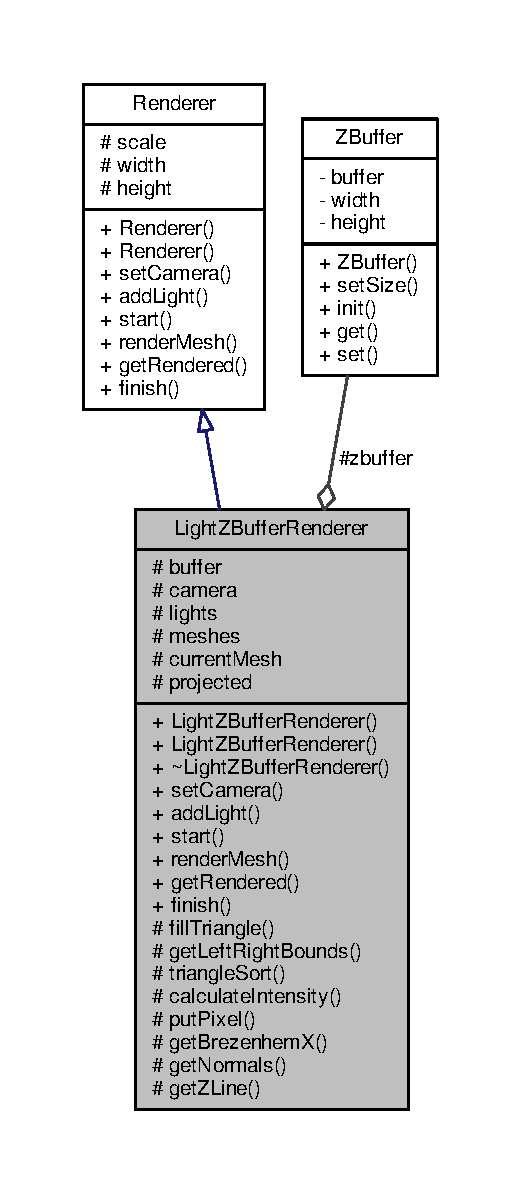
\includegraphics[height=550pt]{db/d8f/class_light_z_buffer_renderer__coll__graph}
\end{center}
\end{figure}
\subsection*{Открытые члены}
\begin{DoxyCompactItemize}
\item 
\hyperlink{class_light_z_buffer_renderer_a6b48dd8c2782308bd742cd43f4185a53}{Light\+Z\+Buffer\+Renderer} ()=default
\item 
\hyperlink{class_light_z_buffer_renderer_ae0d09c94784fc721d926c93a87907a0c}{Light\+Z\+Buffer\+Renderer} (float \hyperlink{class_renderer_aeab228a83d206c55fc73c7a14a0f0761}{scale}, \hyperlink{number_8h_a43d43196463bde49cb067f5c20ab8481}{int32} \hyperlink{class_renderer_ada813defebef120813571bfb6053e88f}{width}, \hyperlink{number_8h_a43d43196463bde49cb067f5c20ab8481}{int32} \hyperlink{class_renderer_ab2e154b790a2d31603f147510c261ac2}{height})
\item 
virtual \hyperlink{class_light_z_buffer_renderer_a8bc0f947c608e08a7094be1b02a27e13}{$\sim$\+Light\+Z\+Buffer\+Renderer} ()
\item 
virtual void \hyperlink{class_light_z_buffer_renderer_acc0d204a38cc6105a7c258b49e5197a4}{set\+Camera} (\hyperlink{camera_8h_a01f929aec8e912be07dca2c1f8d00f67}{Shared\+Camera} value) override
\item 
virtual void \hyperlink{class_light_z_buffer_renderer_a73f101ddbdbb27eb19d6ee719da9bf9a}{add\+Light} (\hyperlink{light_8h_ae1ec32369be93ce20c1e9047a8d388c0}{Shared\+Light}) override
\item 
virtual void \hyperlink{class_light_z_buffer_renderer_a431be9dc219e4d2706c95ada2aca8af6}{start} (\hyperlink{number_8h_a43d43196463bde49cb067f5c20ab8481}{int32} \hyperlink{class_renderer_ada813defebef120813571bfb6053e88f}{width}, \hyperlink{number_8h_a43d43196463bde49cb067f5c20ab8481}{int32} \hyperlink{class_renderer_ab2e154b790a2d31603f147510c261ac2}{height}) override
\item 
virtual void \hyperlink{class_light_z_buffer_renderer_a258b9e41e648b8f6393a39d2935d4d42}{render\+Mesh} (shared\+\_\+ptr$<$ \hyperlink{class_mesh}{Mesh} $>$ mesh) override
\item 
virtual uchar $\ast$ \hyperlink{class_light_z_buffer_renderer_a7e712d8d1b3a7be674efb620ba3ff0ef}{get\+Rendered} () override
\item 
virtual void \hyperlink{class_light_z_buffer_renderer_ad8084c0d5f0b4555900efbeaa81ec066}{finish} () override
\end{DoxyCompactItemize}
\subsection*{Защищенные члены}
\begin{DoxyCompactItemize}
\item 
void \hyperlink{class_light_z_buffer_renderer_a48bc043f59326ca98f2821e96710cd41}{fill\+Triangle} (\hyperlink{class_triangle}{Triangle} \&triangle)
\item 
void \hyperlink{class_light_z_buffer_renderer_a4fa5b867bf1e51f603713631d674cb06}{get\+Left\+Right\+Bounds} (std\+::vector$<$ float $>$ \&lleft, std\+::vector$<$ float $>$ \&lright, std\+::vector$<$ \hyperlink{vec3_8h_a221ad8ea4d9be4111628ee1ca22ee3ba}{Vec3} $>$ \&nleft, std\+::vector$<$ \hyperlink{vec3_8h_a221ad8ea4d9be4111628ee1ca22ee3ba}{Vec3} $>$ \&nright, std\+::vector$<$ float $>$ \&zleft, std\+::vector$<$ float $>$ \&zright, \hyperlink{class_triangle}{Triangle} \&triangle, bool \&swapped)
\item 
void \hyperlink{class_light_z_buffer_renderer_a73dff4db530851b997e468bf73eb98ab}{triangle\+Sort} (const std\+::vector$<$ \hyperlink{vec3_8h_a221ad8ea4d9be4111628ee1ca22ee3ba}{Vec3} $>$ \&vertices, \hyperlink{class_triangle}{Triangle} \&triangle)
\item 
\hyperlink{class_color}{Color} \hyperlink{class_light_z_buffer_renderer_ad22c18963eabaa75aea9e26472e24895}{calculate\+Intensity} (const \hyperlink{vec3_8h_a221ad8ea4d9be4111628ee1ca22ee3ba}{Vec3} \&n, const \hyperlink{vec3_8h_a221ad8ea4d9be4111628ee1ca22ee3ba}{Vec3} \&orig, const \hyperlink{class_color}{Color} \&ka, const \hyperlink{class_color}{Color} \&kd, const \hyperlink{class_color}{Color} \&ks, float ns)
\item 
void \hyperlink{class_light_z_buffer_renderer_a5ab92396f07a122fdd9296d2647d5ba9}{put\+Pixel} (\hyperlink{number_8h_a43d43196463bde49cb067f5c20ab8481}{int32} x, \hyperlink{number_8h_a43d43196463bde49cb067f5c20ab8481}{int32} y, const \hyperlink{class_color}{Color} \&color)
\item 
std\+::vector$<$ float $>$ \hyperlink{class_light_z_buffer_renderer_a8f2e11c38172b8a5da977ab951937055}{get\+BrezenhemX} (const \hyperlink{vec3_8h_a221ad8ea4d9be4111628ee1ca22ee3ba}{Vec3} \&p1, const \hyperlink{vec3_8h_a221ad8ea4d9be4111628ee1ca22ee3ba}{Vec3} \&p2)
\item 
std\+::vector$<$ \hyperlink{vec3_8h_a221ad8ea4d9be4111628ee1ca22ee3ba}{Vec3} $>$ \hyperlink{class_light_z_buffer_renderer_ae37535afff9d52ee46c6be7321bca843}{get\+Normals} (const std\+::vector$<$ float $>$ \&l, const \hyperlink{vec3_8h_a221ad8ea4d9be4111628ee1ca22ee3ba}{Vec3} \&n1, const \hyperlink{vec3_8h_a221ad8ea4d9be4111628ee1ca22ee3ba}{Vec3} \&n2)
\item 
std\+::vector$<$ float $>$ \hyperlink{class_light_z_buffer_renderer_a7ba24d9b0fbd7e05b85bc857d147ff52}{get\+Z\+Line} (const \hyperlink{vec3_8h_a221ad8ea4d9be4111628ee1ca22ee3ba}{Vec3} \&p1, const \hyperlink{vec3_8h_a221ad8ea4d9be4111628ee1ca22ee3ba}{Vec3} \&p2, \hyperlink{number_8h_a43d43196463bde49cb067f5c20ab8481}{int32} n)
\end{DoxyCompactItemize}
\subsection*{Защищенные данные}
\begin{DoxyCompactItemize}
\item 
\hyperlink{class_z_buffer}{Z\+Buffer} \hyperlink{class_light_z_buffer_renderer_ad2acd2dd6506b9847a5ab10405b3a856}{zbuffer}
\item 
uchar $\ast$ \hyperlink{class_light_z_buffer_renderer_adb59e3ede69cc0d7ebf1c203bd01a8fd}{buffer}
\item 
\hyperlink{camera_8h_a01f929aec8e912be07dca2c1f8d00f67}{Shared\+Camera} \hyperlink{class_light_z_buffer_renderer_a0484f1880ff31e965399a77b8795903f}{camera}
\item 
vector$<$ \hyperlink{light_8h_ae1ec32369be93ce20c1e9047a8d388c0}{Shared\+Light} $>$ \hyperlink{class_light_z_buffer_renderer_aa656a2afff0d9f793c6f93000fdc6f88}{lights}
\item 
vector$<$ shared\+\_\+ptr$<$ \hyperlink{class_mesh}{Mesh} $>$ $>$ \hyperlink{class_light_z_buffer_renderer_ab019713ebac78d9b63039a06900f1c76}{meshes}
\item 
shared\+\_\+ptr$<$ \hyperlink{class_mesh}{Mesh} $>$ \hyperlink{class_light_z_buffer_renderer_a7971a31fc4b6ce58e115fa0a3580f46c}{current\+Mesh}
\item 
vector$<$ \hyperlink{vec3_8h_a221ad8ea4d9be4111628ee1ca22ee3ba}{Vec3} $>$ \hyperlink{class_light_z_buffer_renderer_a809ed37dacd61c93f142be3ed674bc6f}{projected}
\end{DoxyCompactItemize}


\subsection{Подробное описание}


См. определение в файле lightzbufferrenderer.\+h строка 9



\subsection{Конструктор(ы)}
\index{Light\+Z\+Buffer\+Renderer@{Light\+Z\+Buffer\+Renderer}!Light\+Z\+Buffer\+Renderer@{Light\+Z\+Buffer\+Renderer}}
\index{Light\+Z\+Buffer\+Renderer@{Light\+Z\+Buffer\+Renderer}!Light\+Z\+Buffer\+Renderer@{Light\+Z\+Buffer\+Renderer}}
\subsubsection[{\texorpdfstring{Light\+Z\+Buffer\+Renderer()=default}{LightZBufferRenderer()=default}}]{\setlength{\rightskip}{0pt plus 5cm}Light\+Z\+Buffer\+Renderer\+::\+Light\+Z\+Buffer\+Renderer (
\begin{DoxyParamCaption}
{}
\end{DoxyParamCaption}
)\hspace{0.3cm}{\ttfamily [default]}}\hypertarget{class_light_z_buffer_renderer_a6b48dd8c2782308bd742cd43f4185a53}{}\label{class_light_z_buffer_renderer_a6b48dd8c2782308bd742cd43f4185a53}
\index{Light\+Z\+Buffer\+Renderer@{Light\+Z\+Buffer\+Renderer}!Light\+Z\+Buffer\+Renderer@{Light\+Z\+Buffer\+Renderer}}
\index{Light\+Z\+Buffer\+Renderer@{Light\+Z\+Buffer\+Renderer}!Light\+Z\+Buffer\+Renderer@{Light\+Z\+Buffer\+Renderer}}
\subsubsection[{\texorpdfstring{Light\+Z\+Buffer\+Renderer(float scale, int32 width, int32 height)}{LightZBufferRenderer(float scale, int32 width, int32 height)}}]{\setlength{\rightskip}{0pt plus 5cm}Light\+Z\+Buffer\+Renderer\+::\+Light\+Z\+Buffer\+Renderer (
\begin{DoxyParamCaption}
\item[{float}]{scale, }
\item[{{\bf int32}}]{width, }
\item[{{\bf int32}}]{height}
\end{DoxyParamCaption}
)}\hypertarget{class_light_z_buffer_renderer_ae0d09c94784fc721d926c93a87907a0c}{}\label{class_light_z_buffer_renderer_ae0d09c94784fc721d926c93a87907a0c}


См. определение в файле lightzbufferrenderer.\+cpp строка 10

\index{Light\+Z\+Buffer\+Renderer@{Light\+Z\+Buffer\+Renderer}!````~Light\+Z\+Buffer\+Renderer@{$\sim$\+Light\+Z\+Buffer\+Renderer}}
\index{````~Light\+Z\+Buffer\+Renderer@{$\sim$\+Light\+Z\+Buffer\+Renderer}!Light\+Z\+Buffer\+Renderer@{Light\+Z\+Buffer\+Renderer}}
\subsubsection[{\texorpdfstring{$\sim$\+Light\+Z\+Buffer\+Renderer()}{~LightZBufferRenderer()}}]{\setlength{\rightskip}{0pt plus 5cm}Light\+Z\+Buffer\+Renderer\+::$\sim$\+Light\+Z\+Buffer\+Renderer (
\begin{DoxyParamCaption}
{}
\end{DoxyParamCaption}
)\hspace{0.3cm}{\ttfamily [virtual]}}\hypertarget{class_light_z_buffer_renderer_a8bc0f947c608e08a7094be1b02a27e13}{}\label{class_light_z_buffer_renderer_a8bc0f947c608e08a7094be1b02a27e13}


См. определение в файле lightzbufferrenderer.\+cpp строка 18



\subsection{Методы}
\index{Light\+Z\+Buffer\+Renderer@{Light\+Z\+Buffer\+Renderer}!add\+Light@{add\+Light}}
\index{add\+Light@{add\+Light}!Light\+Z\+Buffer\+Renderer@{Light\+Z\+Buffer\+Renderer}}
\subsubsection[{\texorpdfstring{add\+Light(\+Shared\+Light) override}{addLight(SharedLight) override}}]{\setlength{\rightskip}{0pt plus 5cm}void Light\+Z\+Buffer\+Renderer\+::add\+Light (
\begin{DoxyParamCaption}
\item[{{\bf Shared\+Light}}]{value}
\end{DoxyParamCaption}
)\hspace{0.3cm}{\ttfamily [override]}, {\ttfamily [virtual]}}\hypertarget{class_light_z_buffer_renderer_a73f101ddbdbb27eb19d6ee719da9bf9a}{}\label{class_light_z_buffer_renderer_a73f101ddbdbb27eb19d6ee719da9bf9a}


Замещает \hyperlink{class_renderer_a000c8a4b55c252ad1353bbd33dc4def9}{Renderer}.



См. определение в файле lightzbufferrenderer.\+cpp строка 30

\index{Light\+Z\+Buffer\+Renderer@{Light\+Z\+Buffer\+Renderer}!calculate\+Intensity@{calculate\+Intensity}}
\index{calculate\+Intensity@{calculate\+Intensity}!Light\+Z\+Buffer\+Renderer@{Light\+Z\+Buffer\+Renderer}}
\subsubsection[{\texorpdfstring{calculate\+Intensity(const Vec3 \&n, const Vec3 \&orig, const Color \&ka, const Color \&kd, const Color \&ks, float ns)}{calculateIntensity(const Vec3 &n, const Vec3 &orig, const Color &ka, const Color &kd, const Color &ks, float ns)}}]{\setlength{\rightskip}{0pt plus 5cm}{\bf Color} Light\+Z\+Buffer\+Renderer\+::calculate\+Intensity (
\begin{DoxyParamCaption}
\item[{const {\bf Vec3} \&}]{n, }
\item[{const {\bf Vec3} \&}]{orig, }
\item[{const {\bf Color} \&}]{ka, }
\item[{const {\bf Color} \&}]{kd, }
\item[{const {\bf Color} \&}]{ks, }
\item[{float}]{ns}
\end{DoxyParamCaption}
)\hspace{0.3cm}{\ttfamily [protected]}}\hypertarget{class_light_z_buffer_renderer_ad22c18963eabaa75aea9e26472e24895}{}\label{class_light_z_buffer_renderer_ad22c18963eabaa75aea9e26472e24895}


См. определение в файле lightzbufferrenderer.\+cpp строка 111

\index{Light\+Z\+Buffer\+Renderer@{Light\+Z\+Buffer\+Renderer}!fill\+Triangle@{fill\+Triangle}}
\index{fill\+Triangle@{fill\+Triangle}!Light\+Z\+Buffer\+Renderer@{Light\+Z\+Buffer\+Renderer}}
\subsubsection[{\texorpdfstring{fill\+Triangle(\+Triangle \&triangle)}{fillTriangle(Triangle &triangle)}}]{\setlength{\rightskip}{0pt plus 5cm}void Light\+Z\+Buffer\+Renderer\+::fill\+Triangle (
\begin{DoxyParamCaption}
\item[{{\bf Triangle} \&}]{triangle}
\end{DoxyParamCaption}
)\hspace{0.3cm}{\ttfamily [protected]}}\hypertarget{class_light_z_buffer_renderer_a48bc043f59326ca98f2821e96710cd41}{}\label{class_light_z_buffer_renderer_a48bc043f59326ca98f2821e96710cd41}


См. определение в файле lightzbufferrenderer.\+cpp строка 144

\index{Light\+Z\+Buffer\+Renderer@{Light\+Z\+Buffer\+Renderer}!finish@{finish}}
\index{finish@{finish}!Light\+Z\+Buffer\+Renderer@{Light\+Z\+Buffer\+Renderer}}
\subsubsection[{\texorpdfstring{finish() override}{finish() override}}]{\setlength{\rightskip}{0pt plus 5cm}void Light\+Z\+Buffer\+Renderer\+::finish (
\begin{DoxyParamCaption}
{}
\end{DoxyParamCaption}
)\hspace{0.3cm}{\ttfamily [override]}, {\ttfamily [virtual]}}\hypertarget{class_light_z_buffer_renderer_ad8084c0d5f0b4555900efbeaa81ec066}{}\label{class_light_z_buffer_renderer_ad8084c0d5f0b4555900efbeaa81ec066}


Замещает \hyperlink{class_renderer_ae8a0a67a993626066a989dbf02ae43f9}{Renderer}.



См. определение в файле lightzbufferrenderer.\+cpp строка 319

\index{Light\+Z\+Buffer\+Renderer@{Light\+Z\+Buffer\+Renderer}!get\+BrezenhemX@{get\+BrezenhemX}}
\index{get\+BrezenhemX@{get\+BrezenhemX}!Light\+Z\+Buffer\+Renderer@{Light\+Z\+Buffer\+Renderer}}
\subsubsection[{\texorpdfstring{get\+Brezenhem\+X(const Vec3 \&p1, const Vec3 \&p2)}{getBrezenhemX(const Vec3 &p1, const Vec3 &p2)}}]{\setlength{\rightskip}{0pt plus 5cm}std\+::vector$<$ float $>$ Light\+Z\+Buffer\+Renderer\+::get\+BrezenhemX (
\begin{DoxyParamCaption}
\item[{const {\bf Vec3} \&}]{p1, }
\item[{const {\bf Vec3} \&}]{p2}
\end{DoxyParamCaption}
)\hspace{0.3cm}{\ttfamily [protected]}}\hypertarget{class_light_z_buffer_renderer_a8f2e11c38172b8a5da977ab951937055}{}\label{class_light_z_buffer_renderer_a8f2e11c38172b8a5da977ab951937055}


См. определение в файле lightzbufferrenderer.\+cpp строка 53

\index{Light\+Z\+Buffer\+Renderer@{Light\+Z\+Buffer\+Renderer}!get\+Left\+Right\+Bounds@{get\+Left\+Right\+Bounds}}
\index{get\+Left\+Right\+Bounds@{get\+Left\+Right\+Bounds}!Light\+Z\+Buffer\+Renderer@{Light\+Z\+Buffer\+Renderer}}
\subsubsection[{\texorpdfstring{get\+Left\+Right\+Bounds(std\+::vector$<$ float $>$ \&lleft, std\+::vector$<$ float $>$ \&lright, std\+::vector$<$ Vec3 $>$ \&nleft, std\+::vector$<$ Vec3 $>$ \&nright, std\+::vector$<$ float $>$ \&zleft, std\+::vector$<$ float $>$ \&zright, Triangle \&triangle, bool \&swapped)}{getLeftRightBounds(std::vector< float > &lleft, std::vector< float > &lright, std::vector< Vec3 > &nleft, std::vector< Vec3 > &nright, std::vector< float > &zleft, std::vector< float > &zright, Triangle &triangle, bool &swapped)}}]{\setlength{\rightskip}{0pt plus 5cm}void Light\+Z\+Buffer\+Renderer\+::get\+Left\+Right\+Bounds (
\begin{DoxyParamCaption}
\item[{std\+::vector$<$ float $>$ \&}]{lleft, }
\item[{std\+::vector$<$ float $>$ \&}]{lright, }
\item[{std\+::vector$<$ {\bf Vec3} $>$ \&}]{nleft, }
\item[{std\+::vector$<$ {\bf Vec3} $>$ \&}]{nright, }
\item[{std\+::vector$<$ float $>$ \&}]{zleft, }
\item[{std\+::vector$<$ float $>$ \&}]{zright, }
\item[{{\bf Triangle} \&}]{triangle, }
\item[{bool \&}]{swapped}
\end{DoxyParamCaption}
)\hspace{0.3cm}{\ttfamily [protected]}}\hypertarget{class_light_z_buffer_renderer_a4fa5b867bf1e51f603713631d674cb06}{}\label{class_light_z_buffer_renderer_a4fa5b867bf1e51f603713631d674cb06}


См. определение в файле lightzbufferrenderer.\+cpp строка 213

\index{Light\+Z\+Buffer\+Renderer@{Light\+Z\+Buffer\+Renderer}!get\+Normals@{get\+Normals}}
\index{get\+Normals@{get\+Normals}!Light\+Z\+Buffer\+Renderer@{Light\+Z\+Buffer\+Renderer}}
\subsubsection[{\texorpdfstring{get\+Normals(const std\+::vector$<$ float $>$ \&l, const Vec3 \&n1, const Vec3 \&n2)}{getNormals(const std::vector< float > &l, const Vec3 &n1, const Vec3 &n2)}}]{\setlength{\rightskip}{0pt plus 5cm}std\+::vector$<$ {\bf Vec3} $>$ Light\+Z\+Buffer\+Renderer\+::get\+Normals (
\begin{DoxyParamCaption}
\item[{const std\+::vector$<$ float $>$ \&}]{l, }
\item[{const {\bf Vec3} \&}]{n1, }
\item[{const {\bf Vec3} \&}]{n2}
\end{DoxyParamCaption}
)\hspace{0.3cm}{\ttfamily [protected]}}\hypertarget{class_light_z_buffer_renderer_ae37535afff9d52ee46c6be7321bca843}{}\label{class_light_z_buffer_renderer_ae37535afff9d52ee46c6be7321bca843}


См. определение в файле lightzbufferrenderer.\+cpp строка 72

\index{Light\+Z\+Buffer\+Renderer@{Light\+Z\+Buffer\+Renderer}!get\+Rendered@{get\+Rendered}}
\index{get\+Rendered@{get\+Rendered}!Light\+Z\+Buffer\+Renderer@{Light\+Z\+Buffer\+Renderer}}
\subsubsection[{\texorpdfstring{get\+Rendered() override}{getRendered() override}}]{\setlength{\rightskip}{0pt plus 5cm}uchar $\ast$ Light\+Z\+Buffer\+Renderer\+::get\+Rendered (
\begin{DoxyParamCaption}
{}
\end{DoxyParamCaption}
)\hspace{0.3cm}{\ttfamily [override]}, {\ttfamily [virtual]}}\hypertarget{class_light_z_buffer_renderer_a7e712d8d1b3a7be674efb620ba3ff0ef}{}\label{class_light_z_buffer_renderer_a7e712d8d1b3a7be674efb620ba3ff0ef}


Замещает \hyperlink{class_renderer_ad3a00c526a6765792b02f328e7a7dad1}{Renderer}.



См. определение в файле lightzbufferrenderer.\+cpp строка 40

\index{Light\+Z\+Buffer\+Renderer@{Light\+Z\+Buffer\+Renderer}!get\+Z\+Line@{get\+Z\+Line}}
\index{get\+Z\+Line@{get\+Z\+Line}!Light\+Z\+Buffer\+Renderer@{Light\+Z\+Buffer\+Renderer}}
\subsubsection[{\texorpdfstring{get\+Z\+Line(const Vec3 \&p1, const Vec3 \&p2, int32 n)}{getZLine(const Vec3 &p1, const Vec3 &p2, int32 n)}}]{\setlength{\rightskip}{0pt plus 5cm}std\+::vector$<$ float $>$ Light\+Z\+Buffer\+Renderer\+::get\+Z\+Line (
\begin{DoxyParamCaption}
\item[{const {\bf Vec3} \&}]{p1, }
\item[{const {\bf Vec3} \&}]{p2, }
\item[{{\bf int32}}]{n}
\end{DoxyParamCaption}
)\hspace{0.3cm}{\ttfamily [protected]}}\hypertarget{class_light_z_buffer_renderer_a7ba24d9b0fbd7e05b85bc857d147ff52}{}\label{class_light_z_buffer_renderer_a7ba24d9b0fbd7e05b85bc857d147ff52}


См. определение в файле lightzbufferrenderer.\+cpp строка 93

\index{Light\+Z\+Buffer\+Renderer@{Light\+Z\+Buffer\+Renderer}!put\+Pixel@{put\+Pixel}}
\index{put\+Pixel@{put\+Pixel}!Light\+Z\+Buffer\+Renderer@{Light\+Z\+Buffer\+Renderer}}
\subsubsection[{\texorpdfstring{put\+Pixel(int32 x, int32 y, const Color \&color)}{putPixel(int32 x, int32 y, const Color &color)}}]{\setlength{\rightskip}{0pt plus 5cm}void Light\+Z\+Buffer\+Renderer\+::put\+Pixel (
\begin{DoxyParamCaption}
\item[{{\bf int32}}]{x, }
\item[{{\bf int32}}]{y, }
\item[{const {\bf Color} \&}]{color}
\end{DoxyParamCaption}
)\hspace{0.3cm}{\ttfamily [protected]}}\hypertarget{class_light_z_buffer_renderer_a5ab92396f07a122fdd9296d2647d5ba9}{}\label{class_light_z_buffer_renderer_a5ab92396f07a122fdd9296d2647d5ba9}


См. определение в файле lightzbufferrenderer.\+cpp строка 45

\index{Light\+Z\+Buffer\+Renderer@{Light\+Z\+Buffer\+Renderer}!render\+Mesh@{render\+Mesh}}
\index{render\+Mesh@{render\+Mesh}!Light\+Z\+Buffer\+Renderer@{Light\+Z\+Buffer\+Renderer}}
\subsubsection[{\texorpdfstring{render\+Mesh(shared\+\_\+ptr$<$ Mesh $>$ mesh) override}{renderMesh(shared_ptr< Mesh > mesh) override}}]{\setlength{\rightskip}{0pt plus 5cm}void Light\+Z\+Buffer\+Renderer\+::render\+Mesh (
\begin{DoxyParamCaption}
\item[{shared\+\_\+ptr$<$ {\bf Mesh} $>$}]{mesh}
\end{DoxyParamCaption}
)\hspace{0.3cm}{\ttfamily [override]}, {\ttfamily [virtual]}}\hypertarget{class_light_z_buffer_renderer_a258b9e41e648b8f6393a39d2935d4d42}{}\label{class_light_z_buffer_renderer_a258b9e41e648b8f6393a39d2935d4d42}


Замещает \hyperlink{class_renderer_a40c3fe3b0e46de69ed563d4b4ca13986}{Renderer}.



См. определение в файле lightzbufferrenderer.\+cpp строка 24

\index{Light\+Z\+Buffer\+Renderer@{Light\+Z\+Buffer\+Renderer}!set\+Camera@{set\+Camera}}
\index{set\+Camera@{set\+Camera}!Light\+Z\+Buffer\+Renderer@{Light\+Z\+Buffer\+Renderer}}
\subsubsection[{\texorpdfstring{set\+Camera(\+Shared\+Camera value) override}{setCamera(SharedCamera value) override}}]{\setlength{\rightskip}{0pt plus 5cm}void Light\+Z\+Buffer\+Renderer\+::set\+Camera (
\begin{DoxyParamCaption}
\item[{{\bf Shared\+Camera}}]{value}
\end{DoxyParamCaption}
)\hspace{0.3cm}{\ttfamily [override]}, {\ttfamily [virtual]}}\hypertarget{class_light_z_buffer_renderer_acc0d204a38cc6105a7c258b49e5197a4}{}\label{class_light_z_buffer_renderer_acc0d204a38cc6105a7c258b49e5197a4}


Замещает \hyperlink{class_renderer_a832ac0e6a4fe1e840e07bd82a405edd6}{Renderer}.



См. определение в файле lightzbufferrenderer.\+cpp строка 35

\index{Light\+Z\+Buffer\+Renderer@{Light\+Z\+Buffer\+Renderer}!start@{start}}
\index{start@{start}!Light\+Z\+Buffer\+Renderer@{Light\+Z\+Buffer\+Renderer}}
\subsubsection[{\texorpdfstring{start(int32 width, int32 height) override}{start(int32 width, int32 height) override}}]{\setlength{\rightskip}{0pt plus 5cm}void Light\+Z\+Buffer\+Renderer\+::start (
\begin{DoxyParamCaption}
\item[{{\bf int32}}]{width, }
\item[{{\bf int32}}]{height}
\end{DoxyParamCaption}
)\hspace{0.3cm}{\ttfamily [override]}, {\ttfamily [virtual]}}\hypertarget{class_light_z_buffer_renderer_a431be9dc219e4d2706c95ada2aca8af6}{}\label{class_light_z_buffer_renderer_a431be9dc219e4d2706c95ada2aca8af6}


Замещает \hyperlink{class_renderer_a78cc00edca00b08d09121065fb4fc771}{Renderer}.



См. определение в файле lightzbufferrenderer.\+cpp строка 301

\index{Light\+Z\+Buffer\+Renderer@{Light\+Z\+Buffer\+Renderer}!triangle\+Sort@{triangle\+Sort}}
\index{triangle\+Sort@{triangle\+Sort}!Light\+Z\+Buffer\+Renderer@{Light\+Z\+Buffer\+Renderer}}
\subsubsection[{\texorpdfstring{triangle\+Sort(const std\+::vector$<$ Vec3 $>$ \&vertices, Triangle \&triangle)}{triangleSort(const std::vector< Vec3 > &vertices, Triangle &triangle)}}]{\setlength{\rightskip}{0pt plus 5cm}void Light\+Z\+Buffer\+Renderer\+::triangle\+Sort (
\begin{DoxyParamCaption}
\item[{const std\+::vector$<$ {\bf Vec3} $>$ \&}]{vertices, }
\item[{{\bf Triangle} \&}]{triangle}
\end{DoxyParamCaption}
)\hspace{0.3cm}{\ttfamily [protected]}}\hypertarget{class_light_z_buffer_renderer_a73dff4db530851b997e468bf73eb98ab}{}\label{class_light_z_buffer_renderer_a73dff4db530851b997e468bf73eb98ab}


См. определение в файле lightzbufferrenderer.\+cpp строка 269



\subsection{Данные класса}
\index{Light\+Z\+Buffer\+Renderer@{Light\+Z\+Buffer\+Renderer}!buffer@{buffer}}
\index{buffer@{buffer}!Light\+Z\+Buffer\+Renderer@{Light\+Z\+Buffer\+Renderer}}
\subsubsection[{\texorpdfstring{buffer}{buffer}}]{\setlength{\rightskip}{0pt plus 5cm}uchar$\ast$ Light\+Z\+Buffer\+Renderer\+::buffer\hspace{0.3cm}{\ttfamily [protected]}}\hypertarget{class_light_z_buffer_renderer_adb59e3ede69cc0d7ebf1c203bd01a8fd}{}\label{class_light_z_buffer_renderer_adb59e3ede69cc0d7ebf1c203bd01a8fd}


См. определение в файле lightzbufferrenderer.\+h строка 43

\index{Light\+Z\+Buffer\+Renderer@{Light\+Z\+Buffer\+Renderer}!camera@{camera}}
\index{camera@{camera}!Light\+Z\+Buffer\+Renderer@{Light\+Z\+Buffer\+Renderer}}
\subsubsection[{\texorpdfstring{camera}{camera}}]{\setlength{\rightskip}{0pt plus 5cm}{\bf Shared\+Camera} Light\+Z\+Buffer\+Renderer\+::camera\hspace{0.3cm}{\ttfamily [protected]}}\hypertarget{class_light_z_buffer_renderer_a0484f1880ff31e965399a77b8795903f}{}\label{class_light_z_buffer_renderer_a0484f1880ff31e965399a77b8795903f}


См. определение в файле lightzbufferrenderer.\+h строка 44

\index{Light\+Z\+Buffer\+Renderer@{Light\+Z\+Buffer\+Renderer}!current\+Mesh@{current\+Mesh}}
\index{current\+Mesh@{current\+Mesh}!Light\+Z\+Buffer\+Renderer@{Light\+Z\+Buffer\+Renderer}}
\subsubsection[{\texorpdfstring{current\+Mesh}{currentMesh}}]{\setlength{\rightskip}{0pt plus 5cm}shared\+\_\+ptr$<${\bf Mesh}$>$ Light\+Z\+Buffer\+Renderer\+::current\+Mesh\hspace{0.3cm}{\ttfamily [protected]}}\hypertarget{class_light_z_buffer_renderer_a7971a31fc4b6ce58e115fa0a3580f46c}{}\label{class_light_z_buffer_renderer_a7971a31fc4b6ce58e115fa0a3580f46c}


См. определение в файле lightzbufferrenderer.\+h строка 49

\index{Light\+Z\+Buffer\+Renderer@{Light\+Z\+Buffer\+Renderer}!lights@{lights}}
\index{lights@{lights}!Light\+Z\+Buffer\+Renderer@{Light\+Z\+Buffer\+Renderer}}
\subsubsection[{\texorpdfstring{lights}{lights}}]{\setlength{\rightskip}{0pt plus 5cm}vector$<${\bf Shared\+Light}$>$ Light\+Z\+Buffer\+Renderer\+::lights\hspace{0.3cm}{\ttfamily [protected]}}\hypertarget{class_light_z_buffer_renderer_aa656a2afff0d9f793c6f93000fdc6f88}{}\label{class_light_z_buffer_renderer_aa656a2afff0d9f793c6f93000fdc6f88}


См. определение в файле lightzbufferrenderer.\+h строка 46

\index{Light\+Z\+Buffer\+Renderer@{Light\+Z\+Buffer\+Renderer}!meshes@{meshes}}
\index{meshes@{meshes}!Light\+Z\+Buffer\+Renderer@{Light\+Z\+Buffer\+Renderer}}
\subsubsection[{\texorpdfstring{meshes}{meshes}}]{\setlength{\rightskip}{0pt plus 5cm}vector$<$shared\+\_\+ptr$<${\bf Mesh}$>$ $>$ Light\+Z\+Buffer\+Renderer\+::meshes\hspace{0.3cm}{\ttfamily [protected]}}\hypertarget{class_light_z_buffer_renderer_ab019713ebac78d9b63039a06900f1c76}{}\label{class_light_z_buffer_renderer_ab019713ebac78d9b63039a06900f1c76}


См. определение в файле lightzbufferrenderer.\+h строка 48

\index{Light\+Z\+Buffer\+Renderer@{Light\+Z\+Buffer\+Renderer}!projected@{projected}}
\index{projected@{projected}!Light\+Z\+Buffer\+Renderer@{Light\+Z\+Buffer\+Renderer}}
\subsubsection[{\texorpdfstring{projected}{projected}}]{\setlength{\rightskip}{0pt plus 5cm}vector$<${\bf Vec3}$>$ Light\+Z\+Buffer\+Renderer\+::projected\hspace{0.3cm}{\ttfamily [protected]}}\hypertarget{class_light_z_buffer_renderer_a809ed37dacd61c93f142be3ed674bc6f}{}\label{class_light_z_buffer_renderer_a809ed37dacd61c93f142be3ed674bc6f}


См. определение в файле lightzbufferrenderer.\+h строка 50

\index{Light\+Z\+Buffer\+Renderer@{Light\+Z\+Buffer\+Renderer}!zbuffer@{zbuffer}}
\index{zbuffer@{zbuffer}!Light\+Z\+Buffer\+Renderer@{Light\+Z\+Buffer\+Renderer}}
\subsubsection[{\texorpdfstring{zbuffer}{zbuffer}}]{\setlength{\rightskip}{0pt plus 5cm}{\bf Z\+Buffer} Light\+Z\+Buffer\+Renderer\+::zbuffer\hspace{0.3cm}{\ttfamily [protected]}}\hypertarget{class_light_z_buffer_renderer_ad2acd2dd6506b9847a5ab10405b3a856}{}\label{class_light_z_buffer_renderer_ad2acd2dd6506b9847a5ab10405b3a856}


См. определение в файле lightzbufferrenderer.\+h строка 42



Объявления и описания членов классов находятся в файлах\+:\begin{DoxyCompactItemize}
\item 
Projects/labs/course\+\_\+project\+\_\+cg/src/animation/\hyperlink{lightzbufferrenderer_8h}{lightzbufferrenderer.\+h}\item 
Projects/labs/course\+\_\+project\+\_\+cg/src/animation/\hyperlink{lightzbufferrenderer_8cpp}{lightzbufferrenderer.\+cpp}\end{DoxyCompactItemize}

\hypertarget{class_line}{}\section{Класс Line}
\label{class_line}\index{Line@{Line}}


{\ttfamily \#include $<$line.\+h$>$}



Граф связей класса Line\+:
\nopagebreak
\begin{figure}[H]
\begin{center}
\leavevmode
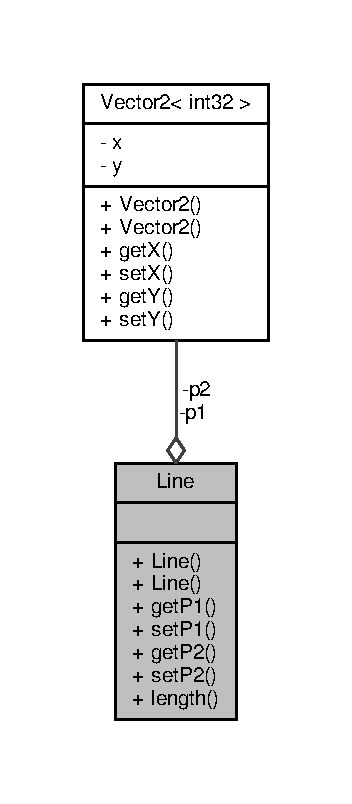
\includegraphics[width=169pt]{da/d45/class_line__coll__graph}
\end{center}
\end{figure}
\subsection*{Открытые члены}
\begin{DoxyCompactItemize}
\item 
\hyperlink{class_line_acc11b8a429d8cdd63ba6803dff5602b3}{Line} ()
\item 
\hyperlink{class_line_aef33536da5a03c1d95e4b113a9dc4ccf}{Line} (const \hyperlink{vec2_8h_a056bf34213a36593f50f333d7653fe1c}{Vec2} \&\hyperlink{class_line_a165376d8bc780a0b0ec7ffe8cd0d700a}{p1}, const \hyperlink{vec2_8h_a056bf34213a36593f50f333d7653fe1c}{Vec2} \&\hyperlink{class_line_a21d0f4b2e7252e222e9d32921ea0162c}{p2})
\item 
\hyperlink{vec2_8h_a056bf34213a36593f50f333d7653fe1c}{Vec2} \hyperlink{class_line_aacff829b7404b0f81bd3001d9332b4a7}{get\+P1} () const 
\item 
void \hyperlink{class_line_a238346a97b448ae7d1156c24dff41224}{set\+P1} (const \hyperlink{vec2_8h_a056bf34213a36593f50f333d7653fe1c}{Vec2} \&value)
\item 
\hyperlink{vec2_8h_a056bf34213a36593f50f333d7653fe1c}{Vec2} \hyperlink{class_line_a51b59fb089fd7a02d3f9d1d9a9a132c7}{get\+P2} () const 
\item 
void \hyperlink{class_line_a9be1bb222db100fe5570558a0ab3bb42}{set\+P2} (const \hyperlink{vec2_8h_a056bf34213a36593f50f333d7653fe1c}{Vec2} \&value)
\item 
float \hyperlink{class_line_ae16899b229d209f5fa5d40049937e030}{length} ()
\end{DoxyCompactItemize}
\subsection*{Закрытые данные}
\begin{DoxyCompactItemize}
\item 
\hyperlink{vec2_8h_a056bf34213a36593f50f333d7653fe1c}{Vec2} \hyperlink{class_line_a165376d8bc780a0b0ec7ffe8cd0d700a}{p1}
\item 
\hyperlink{vec2_8h_a056bf34213a36593f50f333d7653fe1c}{Vec2} \hyperlink{class_line_a21d0f4b2e7252e222e9d32921ea0162c}{p2}
\end{DoxyCompactItemize}


\subsection{Подробное описание}


См. определение в файле line.\+h строка 7



\subsection{Конструктор(ы)}
\index{Line@{Line}!Line@{Line}}
\index{Line@{Line}!Line@{Line}}
\subsubsection[{\texorpdfstring{Line()}{Line()}}]{\setlength{\rightskip}{0pt plus 5cm}Line\+::\+Line (
\begin{DoxyParamCaption}
{}
\end{DoxyParamCaption}
)}\hypertarget{class_line_acc11b8a429d8cdd63ba6803dff5602b3}{}\label{class_line_acc11b8a429d8cdd63ba6803dff5602b3}


См. определение в файле line.\+cpp строка 5

\index{Line@{Line}!Line@{Line}}
\index{Line@{Line}!Line@{Line}}
\subsubsection[{\texorpdfstring{Line(const Vec2 \&p1, const Vec2 \&p2)}{Line(const Vec2 &p1, const Vec2 &p2)}}]{\setlength{\rightskip}{0pt plus 5cm}Line\+::\+Line (
\begin{DoxyParamCaption}
\item[{const {\bf Vec2} \&}]{p1, }
\item[{const {\bf Vec2} \&}]{p2}
\end{DoxyParamCaption}
)}\hypertarget{class_line_aef33536da5a03c1d95e4b113a9dc4ccf}{}\label{class_line_aef33536da5a03c1d95e4b113a9dc4ccf}


См. определение в файле line.\+cpp строка 9



\subsection{Методы}
\index{Line@{Line}!get\+P1@{get\+P1}}
\index{get\+P1@{get\+P1}!Line@{Line}}
\subsubsection[{\texorpdfstring{get\+P1() const }{getP1() const }}]{\setlength{\rightskip}{0pt plus 5cm}{\bf Vec2} Line\+::get\+P1 (
\begin{DoxyParamCaption}
{}
\end{DoxyParamCaption}
) const}\hypertarget{class_line_aacff829b7404b0f81bd3001d9332b4a7}{}\label{class_line_aacff829b7404b0f81bd3001d9332b4a7}


См. определение в файле line.\+cpp строка 15

\index{Line@{Line}!get\+P2@{get\+P2}}
\index{get\+P2@{get\+P2}!Line@{Line}}
\subsubsection[{\texorpdfstring{get\+P2() const }{getP2() const }}]{\setlength{\rightskip}{0pt plus 5cm}{\bf Vec2} Line\+::get\+P2 (
\begin{DoxyParamCaption}
{}
\end{DoxyParamCaption}
) const}\hypertarget{class_line_a51b59fb089fd7a02d3f9d1d9a9a132c7}{}\label{class_line_a51b59fb089fd7a02d3f9d1d9a9a132c7}


См. определение в файле line.\+cpp строка 25

\index{Line@{Line}!length@{length}}
\index{length@{length}!Line@{Line}}
\subsubsection[{\texorpdfstring{length()}{length()}}]{\setlength{\rightskip}{0pt plus 5cm}float Line\+::length (
\begin{DoxyParamCaption}
{}
\end{DoxyParamCaption}
)}\hypertarget{class_line_ae16899b229d209f5fa5d40049937e030}{}\label{class_line_ae16899b229d209f5fa5d40049937e030}


См. определение в файле line.\+cpp строка 35

\index{Line@{Line}!set\+P1@{set\+P1}}
\index{set\+P1@{set\+P1}!Line@{Line}}
\subsubsection[{\texorpdfstring{set\+P1(const Vec2 \&value)}{setP1(const Vec2 &value)}}]{\setlength{\rightskip}{0pt plus 5cm}void Line\+::set\+P1 (
\begin{DoxyParamCaption}
\item[{const {\bf Vec2} \&}]{value}
\end{DoxyParamCaption}
)}\hypertarget{class_line_a238346a97b448ae7d1156c24dff41224}{}\label{class_line_a238346a97b448ae7d1156c24dff41224}


См. определение в файле line.\+cpp строка 20

\index{Line@{Line}!set\+P2@{set\+P2}}
\index{set\+P2@{set\+P2}!Line@{Line}}
\subsubsection[{\texorpdfstring{set\+P2(const Vec2 \&value)}{setP2(const Vec2 &value)}}]{\setlength{\rightskip}{0pt plus 5cm}void Line\+::set\+P2 (
\begin{DoxyParamCaption}
\item[{const {\bf Vec2} \&}]{value}
\end{DoxyParamCaption}
)}\hypertarget{class_line_a9be1bb222db100fe5570558a0ab3bb42}{}\label{class_line_a9be1bb222db100fe5570558a0ab3bb42}


См. определение в файле line.\+cpp строка 30



\subsection{Данные класса}
\index{Line@{Line}!p1@{p1}}
\index{p1@{p1}!Line@{Line}}
\subsubsection[{\texorpdfstring{p1}{p1}}]{\setlength{\rightskip}{0pt plus 5cm}{\bf Vec2} Line\+::p1\hspace{0.3cm}{\ttfamily [private]}}\hypertarget{class_line_a165376d8bc780a0b0ec7ffe8cd0d700a}{}\label{class_line_a165376d8bc780a0b0ec7ffe8cd0d700a}


См. определение в файле line.\+h строка 22

\index{Line@{Line}!p2@{p2}}
\index{p2@{p2}!Line@{Line}}
\subsubsection[{\texorpdfstring{p2}{p2}}]{\setlength{\rightskip}{0pt plus 5cm}{\bf Vec2} Line\+::p2\hspace{0.3cm}{\ttfamily [private]}}\hypertarget{class_line_a21d0f4b2e7252e222e9d32921ea0162c}{}\label{class_line_a21d0f4b2e7252e222e9d32921ea0162c}


См. определение в файле line.\+h строка 23



Объявления и описания членов классов находятся в файлах\+:\begin{DoxyCompactItemize}
\item 
Projects/labs/course\+\_\+project\+\_\+cg/src/math/\hyperlink{line_8h}{line.\+h}\item 
Projects/labs/course\+\_\+project\+\_\+cg/src/math/\hyperlink{line_8cpp}{line.\+cpp}\end{DoxyCompactItemize}

\hypertarget{class_line_transform}{}\section{Класс Line\+Transform}
\label{class_line_transform}\index{Line\+Transform@{Line\+Transform}}


{\ttfamily \#include $<$linetransform.\+h$>$}



Граф наследования\+:Line\+Transform\+:
\nopagebreak
\begin{figure}[H]
\begin{center}
\leavevmode
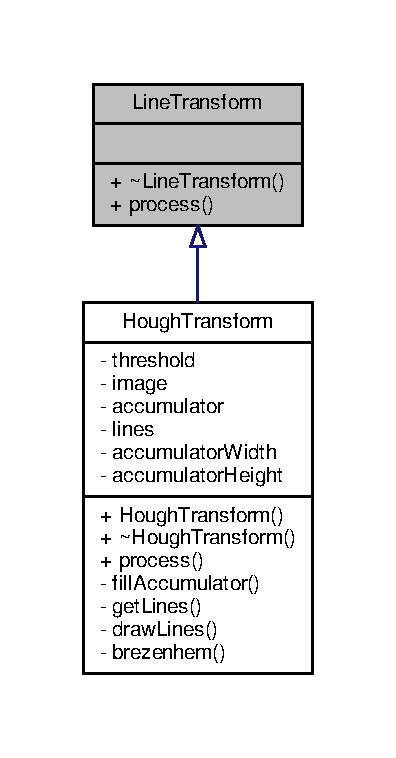
\includegraphics[width=190pt]{da/d01/class_line_transform__inherit__graph}
\end{center}
\end{figure}


Граф связей класса Line\+Transform\+:
\nopagebreak
\begin{figure}[H]
\begin{center}
\leavevmode
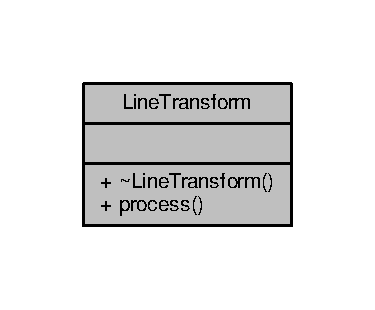
\includegraphics[width=180pt]{d3/d2d/class_line_transform__coll__graph}
\end{center}
\end{figure}
\subsection*{Открытые члены}
\begin{DoxyCompactItemize}
\item 
virtual \hyperlink{class_line_transform_a8398e1a394cfaf6c988c5f2cfc49447d}{$\sim$\+Line\+Transform} ()
\item 
virtual std\+::vector$<$ \hyperlink{class_line}{Line} $>$ \hyperlink{class_line_transform_a391ea9da214224bd3fe428a41c271761}{process} (\hyperlink{class_image}{Image} \&image)=0
\end{DoxyCompactItemize}


\subsection{Подробное описание}


См. определение в файле linetransform.\+h строка 7



\subsection{Конструктор(ы)}
\index{Line\+Transform@{Line\+Transform}!````~Line\+Transform@{$\sim$\+Line\+Transform}}
\index{````~Line\+Transform@{$\sim$\+Line\+Transform}!Line\+Transform@{Line\+Transform}}
\subsubsection[{\texorpdfstring{$\sim$\+Line\+Transform()}{~LineTransform()}}]{\setlength{\rightskip}{0pt plus 5cm}Line\+Transform\+::$\sim$\+Line\+Transform (
\begin{DoxyParamCaption}
{}
\end{DoxyParamCaption}
)\hspace{0.3cm}{\ttfamily [virtual]}}\hypertarget{class_line_transform_a8398e1a394cfaf6c988c5f2cfc49447d}{}\label{class_line_transform_a8398e1a394cfaf6c988c5f2cfc49447d}


См. определение в файле linetransform.\+cpp строка 4



\subsection{Методы}
\index{Line\+Transform@{Line\+Transform}!process@{process}}
\index{process@{process}!Line\+Transform@{Line\+Transform}}
\subsubsection[{\texorpdfstring{process(\+Image \&image)=0}{process(Image &image)=0}}]{\setlength{\rightskip}{0pt plus 5cm}virtual std\+::vector$<${\bf Line}$>$ Line\+Transform\+::process (
\begin{DoxyParamCaption}
\item[{{\bf Image} \&}]{image}
\end{DoxyParamCaption}
)\hspace{0.3cm}{\ttfamily [pure virtual]}}\hypertarget{class_line_transform_a391ea9da214224bd3fe428a41c271761}{}\label{class_line_transform_a391ea9da214224bd3fe428a41c271761}


Замещается в \hyperlink{class_hough_transform_ab10d9e25f492521d6436701107b93fac}{Hough\+Transform}.



Объявления и описания членов классов находятся в файлах\+:\begin{DoxyCompactItemize}
\item 
Projects/labs/course\+\_\+project\+\_\+cg/src/algorithm/linetransform/\hyperlink{linetransform_8h}{linetransform.\+h}\item 
Projects/labs/course\+\_\+project\+\_\+cg/src/algorithm/linetransform/\hyperlink{linetransform_8cpp}{linetransform.\+cpp}\end{DoxyCompactItemize}

\hypertarget{classobjl_1_1_loader}{}\section{Класс objl\+:\+:Loader}
\label{classobjl_1_1_loader}\index{objl\+::\+Loader@{objl\+::\+Loader}}


{\ttfamily \#include $<$objloader.\+h$>$}



Граф связей класса objl\+:\+:Loader\+:
\nopagebreak
\begin{figure}[H]
\begin{center}
\leavevmode
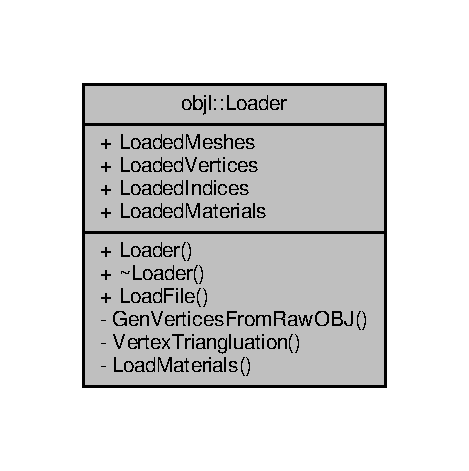
\includegraphics[width=225pt]{dd/d07/classobjl_1_1_loader__coll__graph}
\end{center}
\end{figure}
\subsection*{Открытые члены}
\begin{DoxyCompactItemize}
\item 
\hyperlink{classobjl_1_1_loader_a8ae8d4592c0f727daca80005ae48ea32}{Loader} ()
\item 
\hyperlink{classobjl_1_1_loader_a40d6e6ce91ce09df26a4042605ef4c4c}{$\sim$\+Loader} ()
\item 
bool \hyperlink{classobjl_1_1_loader_a4e3c689962e3ac018d5944f37a791518}{Load\+File} (std\+::string Path)
\end{DoxyCompactItemize}
\subsection*{Открытые атрибуты}
\begin{DoxyCompactItemize}
\item 
std\+::vector$<$ \hyperlink{structobjl_1_1_mesh}{Mesh} $>$ \hyperlink{classobjl_1_1_loader_aba5e73cc2c1d0a917415498723ea5702}{Loaded\+Meshes}
\item 
std\+::vector$<$ \hyperlink{structobjl_1_1_vertex}{Vertex} $>$ \hyperlink{classobjl_1_1_loader_ada15ad9ce70b5c457907be7988436ed5}{Loaded\+Vertices}
\item 
std\+::vector$<$ unsigned int $>$ \hyperlink{classobjl_1_1_loader_a29e18c5a09e82ac44106e282d1acf31a}{Loaded\+Indices}
\item 
std\+::vector$<$ \hyperlink{structobjl_1_1_material}{Material} $>$ \hyperlink{classobjl_1_1_loader_a302204a43746c96f7fe0c72516019f9f}{Loaded\+Materials}
\end{DoxyCompactItemize}
\subsection*{Закрытые члены}
\begin{DoxyCompactItemize}
\item 
void \hyperlink{classobjl_1_1_loader_ac7a2017fa9ec1550c00350f87c7ba93a}{Gen\+Vertices\+From\+Raw\+O\+BJ} (std\+::vector$<$ \hyperlink{structobjl_1_1_vertex}{Vertex} $>$ \&o\+Verts, const std\+::vector$<$ \hyperlink{structobjl_1_1_vector3}{Vector3} $>$ \&i\+Positions, const std\+::vector$<$ \hyperlink{structobjl_1_1_vector2}{Vector2} $>$ \&i\+T\+Coords, const std\+::vector$<$ \hyperlink{structobjl_1_1_vector3}{Vector3} $>$ \&i\+Normals, std\+::string icurline)
\item 
void \hyperlink{classobjl_1_1_loader_a74d527984ea9cb75c7ea1624ee9621b0}{Vertex\+Triangluation} (std\+::vector$<$ unsigned int $>$ \&o\+Indices, const std\+::vector$<$ \hyperlink{structobjl_1_1_vertex}{Vertex} $>$ \&i\+Verts)
\item 
bool \hyperlink{classobjl_1_1_loader_af2f27d60aeb3833d41aec46c6fce5348}{Load\+Materials} (std\+::string path)
\end{DoxyCompactItemize}


\subsection{Подробное описание}


См. определение в файле objloader.\+h строка 388



\subsection{Конструктор(ы)}
\index{objl\+::\+Loader@{objl\+::\+Loader}!Loader@{Loader}}
\index{Loader@{Loader}!objl\+::\+Loader@{objl\+::\+Loader}}
\subsubsection[{\texorpdfstring{Loader()}{Loader()}}]{\setlength{\rightskip}{0pt plus 5cm}objl\+::\+Loader\+::\+Loader (
\begin{DoxyParamCaption}
{}
\end{DoxyParamCaption}
)\hspace{0.3cm}{\ttfamily [inline]}}\hypertarget{classobjl_1_1_loader_a8ae8d4592c0f727daca80005ae48ea32}{}\label{classobjl_1_1_loader_a8ae8d4592c0f727daca80005ae48ea32}


См. определение в файле objloader.\+h строка 392

\index{objl\+::\+Loader@{objl\+::\+Loader}!````~Loader@{$\sim$\+Loader}}
\index{````~Loader@{$\sim$\+Loader}!objl\+::\+Loader@{objl\+::\+Loader}}
\subsubsection[{\texorpdfstring{$\sim$\+Loader()}{~Loader()}}]{\setlength{\rightskip}{0pt plus 5cm}objl\+::\+Loader\+::$\sim$\+Loader (
\begin{DoxyParamCaption}
{}
\end{DoxyParamCaption}
)\hspace{0.3cm}{\ttfamily [inline]}}\hypertarget{classobjl_1_1_loader_a40d6e6ce91ce09df26a4042605ef4c4c}{}\label{classobjl_1_1_loader_a40d6e6ce91ce09df26a4042605ef4c4c}


См. определение в файле objloader.\+h строка 395



\subsection{Методы}
\index{objl\+::\+Loader@{objl\+::\+Loader}!Gen\+Vertices\+From\+Raw\+O\+BJ@{Gen\+Vertices\+From\+Raw\+O\+BJ}}
\index{Gen\+Vertices\+From\+Raw\+O\+BJ@{Gen\+Vertices\+From\+Raw\+O\+BJ}!objl\+::\+Loader@{objl\+::\+Loader}}
\subsubsection[{\texorpdfstring{Gen\+Vertices\+From\+Raw\+O\+B\+J(std\+::vector$<$ Vertex $>$ \&o\+Verts, const std\+::vector$<$ Vector3 $>$ \&i\+Positions, const std\+::vector$<$ Vector2 $>$ \&i\+T\+Coords, const std\+::vector$<$ Vector3 $>$ \&i\+Normals, std\+::string icurline)}{GenVerticesFromRawOBJ(std::vector< Vertex > &oVerts, const std::vector< Vector3 > &iPositions, const std::vector< Vector2 > &iTCoords, const std::vector< Vector3 > &iNormals, std::string icurline)}}]{\setlength{\rightskip}{0pt plus 5cm}void objl\+::\+Loader\+::\+Gen\+Vertices\+From\+Raw\+O\+BJ (
\begin{DoxyParamCaption}
\item[{std\+::vector$<$ {\bf Vertex} $>$ \&}]{o\+Verts, }
\item[{const std\+::vector$<$ {\bf Vector3} $>$ \&}]{i\+Positions, }
\item[{const std\+::vector$<$ {\bf Vector2} $>$ \&}]{i\+T\+Coords, }
\item[{const std\+::vector$<$ {\bf Vector3} $>$ \&}]{i\+Normals, }
\item[{std\+::string}]{icurline}
\end{DoxyParamCaption}
)\hspace{0.3cm}{\ttfamily [inline]}, {\ttfamily [private]}}\hypertarget{classobjl_1_1_loader_ac7a2017fa9ec1550c00350f87c7ba93a}{}\label{classobjl_1_1_loader_ac7a2017fa9ec1550c00350f87c7ba93a}


См. определение в файле objloader.\+h строка 706

\index{objl\+::\+Loader@{objl\+::\+Loader}!Load\+File@{Load\+File}}
\index{Load\+File@{Load\+File}!objl\+::\+Loader@{objl\+::\+Loader}}
\subsubsection[{\texorpdfstring{Load\+File(std\+::string Path)}{LoadFile(std::string Path)}}]{\setlength{\rightskip}{0pt plus 5cm}bool objl\+::\+Loader\+::\+Load\+File (
\begin{DoxyParamCaption}
\item[{std\+::string}]{Path}
\end{DoxyParamCaption}
)\hspace{0.3cm}{\ttfamily [inline]}}\hypertarget{classobjl_1_1_loader_a4e3c689962e3ac018d5944f37a791518}{}\label{classobjl_1_1_loader_a4e3c689962e3ac018d5944f37a791518}


См. определение в файле objloader.\+h строка 406

\index{objl\+::\+Loader@{objl\+::\+Loader}!Load\+Materials@{Load\+Materials}}
\index{Load\+Materials@{Load\+Materials}!objl\+::\+Loader@{objl\+::\+Loader}}
\subsubsection[{\texorpdfstring{Load\+Materials(std\+::string path)}{LoadMaterials(std::string path)}}]{\setlength{\rightskip}{0pt plus 5cm}bool objl\+::\+Loader\+::\+Load\+Materials (
\begin{DoxyParamCaption}
\item[{std\+::string}]{path}
\end{DoxyParamCaption}
)\hspace{0.3cm}{\ttfamily [inline]}, {\ttfamily [private]}}\hypertarget{classobjl_1_1_loader_af2f27d60aeb3833d41aec46c6fce5348}{}\label{classobjl_1_1_loader_af2f27d60aeb3833d41aec46c6fce5348}


См. определение в файле objloader.\+h строка 1035

\index{objl\+::\+Loader@{objl\+::\+Loader}!Vertex\+Triangluation@{Vertex\+Triangluation}}
\index{Vertex\+Triangluation@{Vertex\+Triangluation}!objl\+::\+Loader@{objl\+::\+Loader}}
\subsubsection[{\texorpdfstring{Vertex\+Triangluation(std\+::vector$<$ unsigned int $>$ \&o\+Indices, const std\+::vector$<$ Vertex $>$ \&i\+Verts)}{VertexTriangluation(std::vector< unsigned int > &oIndices, const std::vector< Vertex > &iVerts)}}]{\setlength{\rightskip}{0pt plus 5cm}void objl\+::\+Loader\+::\+Vertex\+Triangluation (
\begin{DoxyParamCaption}
\item[{std\+::vector$<$ unsigned int $>$ \&}]{o\+Indices, }
\item[{const std\+::vector$<$ {\bf Vertex} $>$ \&}]{i\+Verts}
\end{DoxyParamCaption}
)\hspace{0.3cm}{\ttfamily [inline]}, {\ttfamily [private]}}\hypertarget{classobjl_1_1_loader_a74d527984ea9cb75c7ea1624ee9621b0}{}\label{classobjl_1_1_loader_a74d527984ea9cb75c7ea1624ee9621b0}


См. определение в файле objloader.\+h строка 818



\subsection{Данные класса}
\index{objl\+::\+Loader@{objl\+::\+Loader}!Loaded\+Indices@{Loaded\+Indices}}
\index{Loaded\+Indices@{Loaded\+Indices}!objl\+::\+Loader@{objl\+::\+Loader}}
\subsubsection[{\texorpdfstring{Loaded\+Indices}{LoadedIndices}}]{\setlength{\rightskip}{0pt plus 5cm}std\+::vector$<$unsigned int$>$ objl\+::\+Loader\+::\+Loaded\+Indices}\hypertarget{classobjl_1_1_loader_a29e18c5a09e82ac44106e282d1acf31a}{}\label{classobjl_1_1_loader_a29e18c5a09e82ac44106e282d1acf31a}


См. определение в файле objloader.\+h строка 699

\index{objl\+::\+Loader@{objl\+::\+Loader}!Loaded\+Materials@{Loaded\+Materials}}
\index{Loaded\+Materials@{Loaded\+Materials}!objl\+::\+Loader@{objl\+::\+Loader}}
\subsubsection[{\texorpdfstring{Loaded\+Materials}{LoadedMaterials}}]{\setlength{\rightskip}{0pt plus 5cm}std\+::vector$<${\bf Material}$>$ objl\+::\+Loader\+::\+Loaded\+Materials}\hypertarget{classobjl_1_1_loader_a302204a43746c96f7fe0c72516019f9f}{}\label{classobjl_1_1_loader_a302204a43746c96f7fe0c72516019f9f}


См. определение в файле objloader.\+h строка 701

\index{objl\+::\+Loader@{objl\+::\+Loader}!Loaded\+Meshes@{Loaded\+Meshes}}
\index{Loaded\+Meshes@{Loaded\+Meshes}!objl\+::\+Loader@{objl\+::\+Loader}}
\subsubsection[{\texorpdfstring{Loaded\+Meshes}{LoadedMeshes}}]{\setlength{\rightskip}{0pt plus 5cm}std\+::vector$<${\bf Mesh}$>$ objl\+::\+Loader\+::\+Loaded\+Meshes}\hypertarget{classobjl_1_1_loader_aba5e73cc2c1d0a917415498723ea5702}{}\label{classobjl_1_1_loader_aba5e73cc2c1d0a917415498723ea5702}


См. определение в файле objloader.\+h строка 695

\index{objl\+::\+Loader@{objl\+::\+Loader}!Loaded\+Vertices@{Loaded\+Vertices}}
\index{Loaded\+Vertices@{Loaded\+Vertices}!objl\+::\+Loader@{objl\+::\+Loader}}
\subsubsection[{\texorpdfstring{Loaded\+Vertices}{LoadedVertices}}]{\setlength{\rightskip}{0pt plus 5cm}std\+::vector$<${\bf Vertex}$>$ objl\+::\+Loader\+::\+Loaded\+Vertices}\hypertarget{classobjl_1_1_loader_ada15ad9ce70b5c457907be7988436ed5}{}\label{classobjl_1_1_loader_ada15ad9ce70b5c457907be7988436ed5}


См. определение в файле objloader.\+h строка 697



Объявления и описания членов класса находятся в файле\+:\begin{DoxyCompactItemize}
\item 
Projects/labs/course\+\_\+project\+\_\+cg/src/3rdparty/\+Obj\+Loader/\hyperlink{3rdparty_2_obj_loader_2objloader_8h}{objloader.\+h}\end{DoxyCompactItemize}

\hypertarget{class_main_window}{}\section{Класс Main\+Window}
\label{class_main_window}\index{Main\+Window@{Main\+Window}}


{\ttfamily \#include $<$mainwindow.\+h$>$}



Граф наследования\+:Main\+Window\+:
\nopagebreak
\begin{figure}[H]
\begin{center}
\leavevmode
\includegraphics[width=253pt]{de/d4b/class_main_window__inherit__graph}
\end{center}
\end{figure}


Граф связей класса Main\+Window\+:
\nopagebreak
\begin{figure}[H]
\begin{center}
\leavevmode
\includegraphics[height=550pt]{d0/db8/class_main_window__coll__graph}
\end{center}
\end{figure}
\subsection*{Открытые члены}
\begin{DoxyCompactItemize}
\item 
\hyperlink{class_main_window_a8b244be8b7b7db1b08de2a2acb9409db}{Main\+Window} (Q\+Widget $\ast$parent=0)
\item 
\hyperlink{class_main_window_ae98d00a93bc118200eeef9f9bba1dba7}{$\sim$\+Main\+Window} ()
\end{DoxyCompactItemize}
\subsection*{Защищенные члены}
\begin{DoxyCompactItemize}
\item 
void \hyperlink{class_main_window_a8851a931482834eeec527490eedaf20e}{resize\+Event} (Q\+Resize\+Event $\ast$)
\end{DoxyCompactItemize}
\subsection*{Закрытые слоты}
\begin{DoxyCompactItemize}
\item 
void \hyperlink{class_main_window_a444b28f9a298e9e256411f3b428f360c}{on\+\_\+act\+Open\+Image\+\_\+triggered} ()
\item 
void \hyperlink{class_main_window_aa8d88789d920fe1a8094bf0124375e37}{on\+\_\+btn\+Calibrate\+\_\+clicked} ()
\item 
void \hyperlink{class_main_window_ad73256a4d549f57499a168d4ecb29731}{on\+\_\+btn\+Eval\+\_\+clicked} ()
\item 
void \hyperlink{class_main_window_a42f92b00e3336f2efec873fdcb5d612b}{on\+\_\+sld\+Sigma\+\_\+value\+Changed} (int value)
\item 
void \hyperlink{class_main_window_a5f0302c9dadda691baf7db36058dd320}{on\+\_\+sld\+Kernel\+Size\+\_\+value\+Changed} (int value)
\item 
void \hyperlink{class_main_window_a1cd7c221bd2f97f249b13522bcd05aa2}{on\+\_\+sld\+Min\+Thresh\+\_\+value\+Changed} (int value)
\item 
void \hyperlink{class_main_window_a03d260c44d11800d1b6f2653e35bc493}{on\+\_\+sld\+Max\+Thresh\+\_\+value\+Changed} (int value)
\item 
void \hyperlink{class_main_window_adbd6bf1258b5b2b8fd692542f62f0343}{on\+\_\+sld\+Thresh\+\_\+value\+Changed} (int value)
\item 
void \hyperlink{class_main_window_a05932234bd7e1ce4d84a854bd9b1116f}{on\+\_\+act\+Restore\+\_\+triggered} ()
\item 
void \hyperlink{class_main_window_a398b215bc771decd945f2f57755c1378}{on\+\_\+btn\+Gauss\+Apply\+\_\+clicked} ()
\item 
void \hyperlink{class_main_window_a0a67f3153d50bd7b6c460e8cd5bb2f2b}{on\+\_\+btn\+Canny\+Apply\+\_\+clicked} ()
\item 
void \hyperlink{class_main_window_a8475da3b0861fbd81ba3ecdfeabaf706}{on\+\_\+btn\+Hough\+Apply\+\_\+clicked} ()
\item 
void \hyperlink{class_main_window_a566f53b41639cb820cfdd538de49e6c5}{on\+\_\+rbn\+Standard\+\_\+toggled} (bool checked)
\item 
void \hyperlink{class_main_window_a43e6036500db86ce70ce805fadad4676}{on\+\_\+rbn\+Diag\+\_\+toggled} (bool checked)
\item 
void \hyperlink{class_main_window_adbe7e3decb27c0c8120a92c4946d270a}{on\+\_\+act\+Animation\+\_\+triggered} ()
\end{DoxyCompactItemize}
\subsection*{Закрытые члены}
\begin{DoxyCompactItemize}
\item 
void \hyperlink{class_main_window_a288b768c3c21a9171bdc56fe845ece8b}{open\+File} ()
\item 
bool \hyperlink{class_main_window_a1918d23eda34853c378edf6db1d42e34}{load\+File} (const Q\+String \&filename)
\item 
void \hyperlink{class_main_window_ad1d392c319d9debb466d46d0764ff2d2}{set\+Image} (const Q\+Image \&new\+Image)
\item 
void \hyperlink{class_main_window_a58dcc04f752ebec40b339dc7817b50e4}{init\+File\+Dialog} (Q\+File\+Dialog \&dialog, Q\+File\+Dialog\+::\+Accept\+Mode accept\+Mode)
\item 
void \hyperlink{class_main_window_ab435999eabc5f946c138d920a3196ac9}{fit\+To\+Window} ()
\item 
void \hyperlink{class_main_window_aa2ffe303230bdcd17f4ddeafd222ccad}{update\+Actions} ()
\item 
void \hyperlink{class_main_window_a2cf5c71112c73af4937f1f79eb5723ba}{debug\+\_\+set\+Scene} ()
\end{DoxyCompactItemize}
\subsection*{Закрытые данные}
\begin{DoxyCompactItemize}
\item 
\hyperlink{class_animation_window}{Animation\+Window} \hyperlink{class_main_window_aeb8f8bc8e591c09d7c2bd5d3e4a754dc}{w}
\item 
Ui\+::\+Main\+Window $\ast$ \hyperlink{class_main_window_a35466a70ed47252a0191168126a352a5}{ui}
\item 
Q\+Image \hyperlink{class_main_window_a66a1d5b734bad3d2e9e2db622b9950b4}{image}
\item 
\hyperlink{class_cylinder_size_calculator}{Cylinder\+Size\+Calculator} \hyperlink{class_main_window_ab59b6f62b19d0cd5feef140f71655001}{calc}
\item 
int \hyperlink{class_main_window_aa2b6e7a3cfbc2bffb42aa8c74c37ef2b}{state}
\end{DoxyCompactItemize}


\subsection{Подробное описание}


См. определение в файле mainwindow.\+h строка 22



\subsection{Конструктор(ы)}
\index{Main\+Window@{Main\+Window}!Main\+Window@{Main\+Window}}
\index{Main\+Window@{Main\+Window}!Main\+Window@{Main\+Window}}
\subsubsection[{\texorpdfstring{Main\+Window(\+Q\+Widget $\ast$parent=0)}{MainWindow(QWidget *parent=0)}}]{\setlength{\rightskip}{0pt plus 5cm}Main\+Window\+::\+Main\+Window (
\begin{DoxyParamCaption}
\item[{Q\+Widget $\ast$}]{parent = {\ttfamily 0}}
\end{DoxyParamCaption}
)\hspace{0.3cm}{\ttfamily [explicit]}}\hypertarget{class_main_window_a8b244be8b7b7db1b08de2a2acb9409db}{}\label{class_main_window_a8b244be8b7b7db1b08de2a2acb9409db}


См. определение в файле mainwindow.\+cpp строка 15

\index{Main\+Window@{Main\+Window}!````~Main\+Window@{$\sim$\+Main\+Window}}
\index{````~Main\+Window@{$\sim$\+Main\+Window}!Main\+Window@{Main\+Window}}
\subsubsection[{\texorpdfstring{$\sim$\+Main\+Window()}{~MainWindow()}}]{\setlength{\rightskip}{0pt plus 5cm}Main\+Window\+::$\sim$\+Main\+Window (
\begin{DoxyParamCaption}
{}
\end{DoxyParamCaption}
)}\hypertarget{class_main_window_ae98d00a93bc118200eeef9f9bba1dba7}{}\label{class_main_window_ae98d00a93bc118200eeef9f9bba1dba7}


См. определение в файле mainwindow.\+cpp строка 26



\subsection{Методы}
\index{Main\+Window@{Main\+Window}!debug\+\_\+set\+Scene@{debug\+\_\+set\+Scene}}
\index{debug\+\_\+set\+Scene@{debug\+\_\+set\+Scene}!Main\+Window@{Main\+Window}}
\subsubsection[{\texorpdfstring{debug\+\_\+set\+Scene()}{debug_setScene()}}]{\setlength{\rightskip}{0pt plus 5cm}void Main\+Window\+::debug\+\_\+set\+Scene (
\begin{DoxyParamCaption}
{}
\end{DoxyParamCaption}
)\hspace{0.3cm}{\ttfamily [private]}}\hypertarget{class_main_window_a2cf5c71112c73af4937f1f79eb5723ba}{}\label{class_main_window_a2cf5c71112c73af4937f1f79eb5723ba}


См. определение в файле mainwindow.\+cpp строка 117

\index{Main\+Window@{Main\+Window}!fit\+To\+Window@{fit\+To\+Window}}
\index{fit\+To\+Window@{fit\+To\+Window}!Main\+Window@{Main\+Window}}
\subsubsection[{\texorpdfstring{fit\+To\+Window()}{fitToWindow()}}]{\setlength{\rightskip}{0pt plus 5cm}void Main\+Window\+::fit\+To\+Window (
\begin{DoxyParamCaption}
{}
\end{DoxyParamCaption}
)\hspace{0.3cm}{\ttfamily [private]}}\hypertarget{class_main_window_ab435999eabc5f946c138d920a3196ac9}{}\label{class_main_window_ab435999eabc5f946c138d920a3196ac9}
\index{Main\+Window@{Main\+Window}!init\+File\+Dialog@{init\+File\+Dialog}}
\index{init\+File\+Dialog@{init\+File\+Dialog}!Main\+Window@{Main\+Window}}
\subsubsection[{\texorpdfstring{init\+File\+Dialog(\+Q\+File\+Dialog \&dialog, Q\+File\+Dialog\+::\+Accept\+Mode accept\+Mode)}{initFileDialog(QFileDialog &dialog, QFileDialog::AcceptMode acceptMode)}}]{\setlength{\rightskip}{0pt plus 5cm}void Main\+Window\+::init\+File\+Dialog (
\begin{DoxyParamCaption}
\item[{Q\+File\+Dialog \&}]{dialog, }
\item[{Q\+File\+Dialog\+::\+Accept\+Mode}]{accept\+Mode}
\end{DoxyParamCaption}
)\hspace{0.3cm}{\ttfamily [private]}}\hypertarget{class_main_window_a58dcc04f752ebec40b339dc7817b50e4}{}\label{class_main_window_a58dcc04f752ebec40b339dc7817b50e4}


См. определение в файле mainwindow.\+cpp строка 78

\index{Main\+Window@{Main\+Window}!load\+File@{load\+File}}
\index{load\+File@{load\+File}!Main\+Window@{Main\+Window}}
\subsubsection[{\texorpdfstring{load\+File(const Q\+String \&filename)}{loadFile(const QString &filename)}}]{\setlength{\rightskip}{0pt plus 5cm}bool Main\+Window\+::load\+File (
\begin{DoxyParamCaption}
\item[{const Q\+String \&}]{filename}
\end{DoxyParamCaption}
)\hspace{0.3cm}{\ttfamily [private]}}\hypertarget{class_main_window_a1918d23eda34853c378edf6db1d42e34}{}\label{class_main_window_a1918d23eda34853c378edf6db1d42e34}


См. определение в файле mainwindow.\+cpp строка 50

\index{Main\+Window@{Main\+Window}!on\+\_\+act\+Animation\+\_\+triggered@{on\+\_\+act\+Animation\+\_\+triggered}}
\index{on\+\_\+act\+Animation\+\_\+triggered@{on\+\_\+act\+Animation\+\_\+triggered}!Main\+Window@{Main\+Window}}
\subsubsection[{\texorpdfstring{on\+\_\+act\+Animation\+\_\+triggered}{on_actAnimation_triggered}}]{\setlength{\rightskip}{0pt plus 5cm}void Main\+Window\+::on\+\_\+act\+Animation\+\_\+triggered (
\begin{DoxyParamCaption}
{}
\end{DoxyParamCaption}
)\hspace{0.3cm}{\ttfamily [private]}, {\ttfamily [slot]}}\hypertarget{class_main_window_adbe7e3decb27c0c8120a92c4946d270a}{}\label{class_main_window_adbe7e3decb27c0c8120a92c4946d270a}


См. определение в файле mainwindow.\+cpp строка 287

\index{Main\+Window@{Main\+Window}!on\+\_\+act\+Open\+Image\+\_\+triggered@{on\+\_\+act\+Open\+Image\+\_\+triggered}}
\index{on\+\_\+act\+Open\+Image\+\_\+triggered@{on\+\_\+act\+Open\+Image\+\_\+triggered}!Main\+Window@{Main\+Window}}
\subsubsection[{\texorpdfstring{on\+\_\+act\+Open\+Image\+\_\+triggered}{on_actOpenImage_triggered}}]{\setlength{\rightskip}{0pt plus 5cm}void Main\+Window\+::on\+\_\+act\+Open\+Image\+\_\+triggered (
\begin{DoxyParamCaption}
{}
\end{DoxyParamCaption}
)\hspace{0.3cm}{\ttfamily [private]}, {\ttfamily [slot]}}\hypertarget{class_main_window_a444b28f9a298e9e256411f3b428f360c}{}\label{class_main_window_a444b28f9a298e9e256411f3b428f360c}


См. определение в файле mainwindow.\+cpp строка 36

\index{Main\+Window@{Main\+Window}!on\+\_\+act\+Restore\+\_\+triggered@{on\+\_\+act\+Restore\+\_\+triggered}}
\index{on\+\_\+act\+Restore\+\_\+triggered@{on\+\_\+act\+Restore\+\_\+triggered}!Main\+Window@{Main\+Window}}
\subsubsection[{\texorpdfstring{on\+\_\+act\+Restore\+\_\+triggered}{on_actRestore_triggered}}]{\setlength{\rightskip}{0pt plus 5cm}void Main\+Window\+::on\+\_\+act\+Restore\+\_\+triggered (
\begin{DoxyParamCaption}
{}
\end{DoxyParamCaption}
)\hspace{0.3cm}{\ttfamily [private]}, {\ttfamily [slot]}}\hypertarget{class_main_window_a05932234bd7e1ce4d84a854bd9b1116f}{}\label{class_main_window_a05932234bd7e1ce4d84a854bd9b1116f}


См. определение в файле mainwindow.\+cpp строка 223

\index{Main\+Window@{Main\+Window}!on\+\_\+btn\+Calibrate\+\_\+clicked@{on\+\_\+btn\+Calibrate\+\_\+clicked}}
\index{on\+\_\+btn\+Calibrate\+\_\+clicked@{on\+\_\+btn\+Calibrate\+\_\+clicked}!Main\+Window@{Main\+Window}}
\subsubsection[{\texorpdfstring{on\+\_\+btn\+Calibrate\+\_\+clicked}{on_btnCalibrate_clicked}}]{\setlength{\rightskip}{0pt plus 5cm}void Main\+Window\+::on\+\_\+btn\+Calibrate\+\_\+clicked (
\begin{DoxyParamCaption}
{}
\end{DoxyParamCaption}
)\hspace{0.3cm}{\ttfamily [private]}, {\ttfamily [slot]}}\hypertarget{class_main_window_aa8d88789d920fe1a8094bf0124375e37}{}\label{class_main_window_aa8d88789d920fe1a8094bf0124375e37}


См. определение в файле mainwindow.\+cpp строка 122

\index{Main\+Window@{Main\+Window}!on\+\_\+btn\+Canny\+Apply\+\_\+clicked@{on\+\_\+btn\+Canny\+Apply\+\_\+clicked}}
\index{on\+\_\+btn\+Canny\+Apply\+\_\+clicked@{on\+\_\+btn\+Canny\+Apply\+\_\+clicked}!Main\+Window@{Main\+Window}}
\subsubsection[{\texorpdfstring{on\+\_\+btn\+Canny\+Apply\+\_\+clicked}{on_btnCannyApply_clicked}}]{\setlength{\rightskip}{0pt plus 5cm}void Main\+Window\+::on\+\_\+btn\+Canny\+Apply\+\_\+clicked (
\begin{DoxyParamCaption}
{}
\end{DoxyParamCaption}
)\hspace{0.3cm}{\ttfamily [private]}, {\ttfamily [slot]}}\hypertarget{class_main_window_a0a67f3153d50bd7b6c460e8cd5bb2f2b}{}\label{class_main_window_a0a67f3153d50bd7b6c460e8cd5bb2f2b}


См. определение в файле mainwindow.\+cpp строка 240

\index{Main\+Window@{Main\+Window}!on\+\_\+btn\+Eval\+\_\+clicked@{on\+\_\+btn\+Eval\+\_\+clicked}}
\index{on\+\_\+btn\+Eval\+\_\+clicked@{on\+\_\+btn\+Eval\+\_\+clicked}!Main\+Window@{Main\+Window}}
\subsubsection[{\texorpdfstring{on\+\_\+btn\+Eval\+\_\+clicked}{on_btnEval_clicked}}]{\setlength{\rightskip}{0pt plus 5cm}void Main\+Window\+::on\+\_\+btn\+Eval\+\_\+clicked (
\begin{DoxyParamCaption}
{}
\end{DoxyParamCaption}
)\hspace{0.3cm}{\ttfamily [private]}, {\ttfamily [slot]}}\hypertarget{class_main_window_ad73256a4d549f57499a168d4ecb29731}{}\label{class_main_window_ad73256a4d549f57499a168d4ecb29731}


См. определение в файле mainwindow.\+cpp строка 148

\index{Main\+Window@{Main\+Window}!on\+\_\+btn\+Gauss\+Apply\+\_\+clicked@{on\+\_\+btn\+Gauss\+Apply\+\_\+clicked}}
\index{on\+\_\+btn\+Gauss\+Apply\+\_\+clicked@{on\+\_\+btn\+Gauss\+Apply\+\_\+clicked}!Main\+Window@{Main\+Window}}
\subsubsection[{\texorpdfstring{on\+\_\+btn\+Gauss\+Apply\+\_\+clicked}{on_btnGaussApply_clicked}}]{\setlength{\rightskip}{0pt plus 5cm}void Main\+Window\+::on\+\_\+btn\+Gauss\+Apply\+\_\+clicked (
\begin{DoxyParamCaption}
{}
\end{DoxyParamCaption}
)\hspace{0.3cm}{\ttfamily [private]}, {\ttfamily [slot]}}\hypertarget{class_main_window_a398b215bc771decd945f2f57755c1378}{}\label{class_main_window_a398b215bc771decd945f2f57755c1378}


См. определение в файле mainwindow.\+cpp строка 228

\index{Main\+Window@{Main\+Window}!on\+\_\+btn\+Hough\+Apply\+\_\+clicked@{on\+\_\+btn\+Hough\+Apply\+\_\+clicked}}
\index{on\+\_\+btn\+Hough\+Apply\+\_\+clicked@{on\+\_\+btn\+Hough\+Apply\+\_\+clicked}!Main\+Window@{Main\+Window}}
\subsubsection[{\texorpdfstring{on\+\_\+btn\+Hough\+Apply\+\_\+clicked}{on_btnHoughApply_clicked}}]{\setlength{\rightskip}{0pt plus 5cm}void Main\+Window\+::on\+\_\+btn\+Hough\+Apply\+\_\+clicked (
\begin{DoxyParamCaption}
{}
\end{DoxyParamCaption}
)\hspace{0.3cm}{\ttfamily [private]}, {\ttfamily [slot]}}\hypertarget{class_main_window_a8475da3b0861fbd81ba3ecdfeabaf706}{}\label{class_main_window_a8475da3b0861fbd81ba3ecdfeabaf706}


См. определение в файле mainwindow.\+cpp строка 254

\index{Main\+Window@{Main\+Window}!on\+\_\+rbn\+Diag\+\_\+toggled@{on\+\_\+rbn\+Diag\+\_\+toggled}}
\index{on\+\_\+rbn\+Diag\+\_\+toggled@{on\+\_\+rbn\+Diag\+\_\+toggled}!Main\+Window@{Main\+Window}}
\subsubsection[{\texorpdfstring{on\+\_\+rbn\+Diag\+\_\+toggled}{on_rbnDiag_toggled}}]{\setlength{\rightskip}{0pt plus 5cm}void Main\+Window\+::on\+\_\+rbn\+Diag\+\_\+toggled (
\begin{DoxyParamCaption}
\item[{bool}]{checked}
\end{DoxyParamCaption}
)\hspace{0.3cm}{\ttfamily [private]}, {\ttfamily [slot]}}\hypertarget{class_main_window_a43e6036500db86ce70ce805fadad4676}{}\label{class_main_window_a43e6036500db86ce70ce805fadad4676}


См. определение в файле mainwindow.\+cpp строка 278

\index{Main\+Window@{Main\+Window}!on\+\_\+rbn\+Standard\+\_\+toggled@{on\+\_\+rbn\+Standard\+\_\+toggled}}
\index{on\+\_\+rbn\+Standard\+\_\+toggled@{on\+\_\+rbn\+Standard\+\_\+toggled}!Main\+Window@{Main\+Window}}
\subsubsection[{\texorpdfstring{on\+\_\+rbn\+Standard\+\_\+toggled}{on_rbnStandard_toggled}}]{\setlength{\rightskip}{0pt plus 5cm}void Main\+Window\+::on\+\_\+rbn\+Standard\+\_\+toggled (
\begin{DoxyParamCaption}
\item[{bool}]{checked}
\end{DoxyParamCaption}
)\hspace{0.3cm}{\ttfamily [private]}, {\ttfamily [slot]}}\hypertarget{class_main_window_a566f53b41639cb820cfdd538de49e6c5}{}\label{class_main_window_a566f53b41639cb820cfdd538de49e6c5}


См. определение в файле mainwindow.\+cpp строка 269

\index{Main\+Window@{Main\+Window}!on\+\_\+sld\+Kernel\+Size\+\_\+value\+Changed@{on\+\_\+sld\+Kernel\+Size\+\_\+value\+Changed}}
\index{on\+\_\+sld\+Kernel\+Size\+\_\+value\+Changed@{on\+\_\+sld\+Kernel\+Size\+\_\+value\+Changed}!Main\+Window@{Main\+Window}}
\subsubsection[{\texorpdfstring{on\+\_\+sld\+Kernel\+Size\+\_\+value\+Changed}{on_sldKernelSize_valueChanged}}]{\setlength{\rightskip}{0pt plus 5cm}void Main\+Window\+::on\+\_\+sld\+Kernel\+Size\+\_\+value\+Changed (
\begin{DoxyParamCaption}
\item[{int}]{value}
\end{DoxyParamCaption}
)\hspace{0.3cm}{\ttfamily [private]}, {\ttfamily [slot]}}\hypertarget{class_main_window_a5f0302c9dadda691baf7db36058dd320}{}\label{class_main_window_a5f0302c9dadda691baf7db36058dd320}


См. определение в файле mainwindow.\+cpp строка 178

\index{Main\+Window@{Main\+Window}!on\+\_\+sld\+Max\+Thresh\+\_\+value\+Changed@{on\+\_\+sld\+Max\+Thresh\+\_\+value\+Changed}}
\index{on\+\_\+sld\+Max\+Thresh\+\_\+value\+Changed@{on\+\_\+sld\+Max\+Thresh\+\_\+value\+Changed}!Main\+Window@{Main\+Window}}
\subsubsection[{\texorpdfstring{on\+\_\+sld\+Max\+Thresh\+\_\+value\+Changed}{on_sldMaxThresh_valueChanged}}]{\setlength{\rightskip}{0pt plus 5cm}void Main\+Window\+::on\+\_\+sld\+Max\+Thresh\+\_\+value\+Changed (
\begin{DoxyParamCaption}
\item[{int}]{value}
\end{DoxyParamCaption}
)\hspace{0.3cm}{\ttfamily [private]}, {\ttfamily [slot]}}\hypertarget{class_main_window_a03d260c44d11800d1b6f2653e35bc493}{}\label{class_main_window_a03d260c44d11800d1b6f2653e35bc493}


См. определение в файле mainwindow.\+cpp строка 204

\index{Main\+Window@{Main\+Window}!on\+\_\+sld\+Min\+Thresh\+\_\+value\+Changed@{on\+\_\+sld\+Min\+Thresh\+\_\+value\+Changed}}
\index{on\+\_\+sld\+Min\+Thresh\+\_\+value\+Changed@{on\+\_\+sld\+Min\+Thresh\+\_\+value\+Changed}!Main\+Window@{Main\+Window}}
\subsubsection[{\texorpdfstring{on\+\_\+sld\+Min\+Thresh\+\_\+value\+Changed}{on_sldMinThresh_valueChanged}}]{\setlength{\rightskip}{0pt plus 5cm}void Main\+Window\+::on\+\_\+sld\+Min\+Thresh\+\_\+value\+Changed (
\begin{DoxyParamCaption}
\item[{int}]{value}
\end{DoxyParamCaption}
)\hspace{0.3cm}{\ttfamily [private]}, {\ttfamily [slot]}}\hypertarget{class_main_window_a1cd7c221bd2f97f249b13522bcd05aa2}{}\label{class_main_window_a1cd7c221bd2f97f249b13522bcd05aa2}


См. определение в файле mainwindow.\+cpp строка 191

\index{Main\+Window@{Main\+Window}!on\+\_\+sld\+Sigma\+\_\+value\+Changed@{on\+\_\+sld\+Sigma\+\_\+value\+Changed}}
\index{on\+\_\+sld\+Sigma\+\_\+value\+Changed@{on\+\_\+sld\+Sigma\+\_\+value\+Changed}!Main\+Window@{Main\+Window}}
\subsubsection[{\texorpdfstring{on\+\_\+sld\+Sigma\+\_\+value\+Changed}{on_sldSigma_valueChanged}}]{\setlength{\rightskip}{0pt plus 5cm}void Main\+Window\+::on\+\_\+sld\+Sigma\+\_\+value\+Changed (
\begin{DoxyParamCaption}
\item[{int}]{value}
\end{DoxyParamCaption}
)\hspace{0.3cm}{\ttfamily [private]}, {\ttfamily [slot]}}\hypertarget{class_main_window_a42f92b00e3336f2efec873fdcb5d612b}{}\label{class_main_window_a42f92b00e3336f2efec873fdcb5d612b}


См. определение в файле mainwindow.\+cpp строка 166

\index{Main\+Window@{Main\+Window}!on\+\_\+sld\+Thresh\+\_\+value\+Changed@{on\+\_\+sld\+Thresh\+\_\+value\+Changed}}
\index{on\+\_\+sld\+Thresh\+\_\+value\+Changed@{on\+\_\+sld\+Thresh\+\_\+value\+Changed}!Main\+Window@{Main\+Window}}
\subsubsection[{\texorpdfstring{on\+\_\+sld\+Thresh\+\_\+value\+Changed}{on_sldThresh_valueChanged}}]{\setlength{\rightskip}{0pt plus 5cm}void Main\+Window\+::on\+\_\+sld\+Thresh\+\_\+value\+Changed (
\begin{DoxyParamCaption}
\item[{int}]{value}
\end{DoxyParamCaption}
)\hspace{0.3cm}{\ttfamily [private]}, {\ttfamily [slot]}}\hypertarget{class_main_window_adbd6bf1258b5b2b8fd692542f62f0343}{}\label{class_main_window_adbd6bf1258b5b2b8fd692542f62f0343}


См. определение в файле mainwindow.\+cpp строка 217

\index{Main\+Window@{Main\+Window}!open\+File@{open\+File}}
\index{open\+File@{open\+File}!Main\+Window@{Main\+Window}}
\subsubsection[{\texorpdfstring{open\+File()}{openFile()}}]{\setlength{\rightskip}{0pt plus 5cm}void Main\+Window\+::open\+File (
\begin{DoxyParamCaption}
{}
\end{DoxyParamCaption}
)\hspace{0.3cm}{\ttfamily [private]}}\hypertarget{class_main_window_a288b768c3c21a9171bdc56fe845ece8b}{}\label{class_main_window_a288b768c3c21a9171bdc56fe845ece8b}


См. определение в файле mainwindow.\+cpp строка 41

\index{Main\+Window@{Main\+Window}!resize\+Event@{resize\+Event}}
\index{resize\+Event@{resize\+Event}!Main\+Window@{Main\+Window}}
\subsubsection[{\texorpdfstring{resize\+Event(\+Q\+Resize\+Event $\ast$)}{resizeEvent(QResizeEvent *)}}]{\setlength{\rightskip}{0pt plus 5cm}void Main\+Window\+::resize\+Event (
\begin{DoxyParamCaption}
\item[{Q\+Resize\+Event $\ast$}]{}
\end{DoxyParamCaption}
)\hspace{0.3cm}{\ttfamily [protected]}}\hypertarget{class_main_window_a8851a931482834eeec527490eedaf20e}{}\label{class_main_window_a8851a931482834eeec527490eedaf20e}


См. определение в файле mainwindow.\+cpp строка 31

\index{Main\+Window@{Main\+Window}!set\+Image@{set\+Image}}
\index{set\+Image@{set\+Image}!Main\+Window@{Main\+Window}}
\subsubsection[{\texorpdfstring{set\+Image(const Q\+Image \&new\+Image)}{setImage(const QImage &newImage)}}]{\setlength{\rightskip}{0pt plus 5cm}void Main\+Window\+::set\+Image (
\begin{DoxyParamCaption}
\item[{const Q\+Image \&}]{new\+Image}
\end{DoxyParamCaption}
)\hspace{0.3cm}{\ttfamily [private]}}\hypertarget{class_main_window_ad1d392c319d9debb466d46d0764ff2d2}{}\label{class_main_window_ad1d392c319d9debb466d46d0764ff2d2}


См. определение в файле mainwindow.\+cpp строка 71

\index{Main\+Window@{Main\+Window}!update\+Actions@{update\+Actions}}
\index{update\+Actions@{update\+Actions}!Main\+Window@{Main\+Window}}
\subsubsection[{\texorpdfstring{update\+Actions()}{updateActions()}}]{\setlength{\rightskip}{0pt plus 5cm}void Main\+Window\+::update\+Actions (
\begin{DoxyParamCaption}
{}
\end{DoxyParamCaption}
)\hspace{0.3cm}{\ttfamily [private]}}\hypertarget{class_main_window_aa2ffe303230bdcd17f4ddeafd222ccad}{}\label{class_main_window_aa2ffe303230bdcd17f4ddeafd222ccad}


См. определение в файле mainwindow.\+cpp строка 113



\subsection{Данные класса}
\index{Main\+Window@{Main\+Window}!calc@{calc}}
\index{calc@{calc}!Main\+Window@{Main\+Window}}
\subsubsection[{\texorpdfstring{calc}{calc}}]{\setlength{\rightskip}{0pt plus 5cm}{\bf Cylinder\+Size\+Calculator} Main\+Window\+::calc\hspace{0.3cm}{\ttfamily [private]}}\hypertarget{class_main_window_ab59b6f62b19d0cd5feef140f71655001}{}\label{class_main_window_ab59b6f62b19d0cd5feef140f71655001}


См. определение в файле mainwindow.\+h строка 78

\index{Main\+Window@{Main\+Window}!image@{image}}
\index{image@{image}!Main\+Window@{Main\+Window}}
\subsubsection[{\texorpdfstring{image}{image}}]{\setlength{\rightskip}{0pt plus 5cm}Q\+Image Main\+Window\+::image\hspace{0.3cm}{\ttfamily [private]}}\hypertarget{class_main_window_a66a1d5b734bad3d2e9e2db622b9950b4}{}\label{class_main_window_a66a1d5b734bad3d2e9e2db622b9950b4}


См. определение в файле mainwindow.\+h строка 76

\index{Main\+Window@{Main\+Window}!state@{state}}
\index{state@{state}!Main\+Window@{Main\+Window}}
\subsubsection[{\texorpdfstring{state}{state}}]{\setlength{\rightskip}{0pt plus 5cm}int Main\+Window\+::state\hspace{0.3cm}{\ttfamily [private]}}\hypertarget{class_main_window_aa2b6e7a3cfbc2bffb42aa8c74c37ef2b}{}\label{class_main_window_aa2b6e7a3cfbc2bffb42aa8c74c37ef2b}


См. определение в файле mainwindow.\+h строка 80

\index{Main\+Window@{Main\+Window}!ui@{ui}}
\index{ui@{ui}!Main\+Window@{Main\+Window}}
\subsubsection[{\texorpdfstring{ui}{ui}}]{\setlength{\rightskip}{0pt plus 5cm}Ui\+::\+Main\+Window$\ast$ Main\+Window\+::ui\hspace{0.3cm}{\ttfamily [private]}}\hypertarget{class_main_window_a35466a70ed47252a0191168126a352a5}{}\label{class_main_window_a35466a70ed47252a0191168126a352a5}


См. определение в файле mainwindow.\+h строка 75

\index{Main\+Window@{Main\+Window}!w@{w}}
\index{w@{w}!Main\+Window@{Main\+Window}}
\subsubsection[{\texorpdfstring{w}{w}}]{\setlength{\rightskip}{0pt plus 5cm}{\bf Animation\+Window} Main\+Window\+::w\hspace{0.3cm}{\ttfamily [private]}}\hypertarget{class_main_window_aeb8f8bc8e591c09d7c2bd5d3e4a754dc}{}\label{class_main_window_aeb8f8bc8e591c09d7c2bd5d3e4a754dc}


См. определение в файле mainwindow.\+h строка 74



Объявления и описания членов классов находятся в файлах\+:\begin{DoxyCompactItemize}
\item 
Projects/labs/course\+\_\+project\+\_\+cg/src/\hyperlink{mainwindow_8h}{mainwindow.\+h}\item 
Projects/labs/course\+\_\+project\+\_\+cg/src/\hyperlink{mainwindow_8cpp}{mainwindow.\+cpp}\end{DoxyCompactItemize}

\hypertarget{class_material}{}\section{Класс Material}
\label{class_material}\index{Material@{Material}}


{\ttfamily \#include $<$meshdata.\+h$>$}



Граф связей класса Material\+:
\nopagebreak
\begin{figure}[H]
\begin{center}
\leavevmode
\includegraphics[height=550pt]{d5/dad/class_material__coll__graph}
\end{center}
\end{figure}
\subsection*{Открытые члены}
\begin{DoxyCompactItemize}
\item 
\hyperlink{class_material_a6059ec72855855b11672ff25962e9336}{Material} ()=default
\item 
\hyperlink{class_material_ac71c087b6f2dcbf130e19e38067a7a5b}{Material} (const \hyperlink{class_color}{Color} \&\hyperlink{class_material_a93cc771f8b2e9d1f273465e25504ea7b}{ka}, const \hyperlink{class_color}{Color} \&\hyperlink{class_material_a42e6838a32f4a6b54a62a01afc4a1cdb}{kd}, const \hyperlink{class_color}{Color} \&\hyperlink{class_material_a986cb019dc23c99fc139b16793c1ddb5}{ks}, float \hyperlink{class_material_a49335919c5596c4523f71be7f01bdf9d}{ns}, float \hyperlink{class_material_a9132d1f6cc468abe6c40659962e06236}{ni}, float \hyperlink{class_material_a72cb289b8dccb7a08e0b0f7880a92803}{d})
\item 
const \hyperlink{class_color}{Color} \& \hyperlink{class_material_a58208d6d0a2debccac4739af6ba61b7b}{get\+Ka} ()
\item 
void \hyperlink{class_material_af4bc3531d699fb7b7a06253d674d0ede}{set\+Ka} (const \hyperlink{class_color}{Color} \&value)
\item 
const \hyperlink{class_color}{Color} \& \hyperlink{class_material_ad89eb0c9b9d729e918a91d7a621afe10}{get\+Kd} ()
\item 
void \hyperlink{class_material_ab31df4f79c03f8863c96dd748b9d2069}{set\+Kd} (const \hyperlink{class_color}{Color} \&value)
\item 
const \hyperlink{class_color}{Color} \& \hyperlink{class_material_ad03edbeaa265fc4aa796904b7f314e86}{get\+Ks} ()
\item 
void \hyperlink{class_material_a0333444c1bfe41998957f56319481f23}{set\+Ks} (const \hyperlink{class_color}{Color} \&value)
\item 
float \hyperlink{class_material_a8843ba8fa8d3e8fb3e04d6a7553408ea}{get\+Ns} () const 
\item 
void \hyperlink{class_material_a46bf0fa68e2bf6da38f360eaecc8bd13}{set\+Ns} (float value)
\item 
float \hyperlink{class_material_afe38fa1be1b3f608ff08414ccc99d539}{get\+Ni} () const 
\item 
void \hyperlink{class_material_a1d41d55723411069d7774c3ae2b33bc8}{set\+Ni} (float value)
\item 
float \hyperlink{class_material_ae8fef701b92d7ca4ddb3761dd2133fec}{getD} () const 
\item 
void \hyperlink{class_material_a7729d3679891dd4394c1468c0a338a01}{setD} (float value)
\end{DoxyCompactItemize}
\subsection*{Закрытые данные}
\begin{DoxyCompactItemize}
\item 
\hyperlink{class_color}{Color} \hyperlink{class_material_a93cc771f8b2e9d1f273465e25504ea7b}{ka}
\item 
\hyperlink{class_color}{Color} \hyperlink{class_material_a42e6838a32f4a6b54a62a01afc4a1cdb}{kd}
\item 
\hyperlink{class_color}{Color} \hyperlink{class_material_a986cb019dc23c99fc139b16793c1ddb5}{ks}
\item 
float \hyperlink{class_material_a49335919c5596c4523f71be7f01bdf9d}{ns}
\item 
float \hyperlink{class_material_a9132d1f6cc468abe6c40659962e06236}{ni}
\item 
float \hyperlink{class_material_a72cb289b8dccb7a08e0b0f7880a92803}{d}
\end{DoxyCompactItemize}


\subsection{Подробное описание}


См. определение в файле meshdata.\+h строка 52



\subsection{Конструктор(ы)}
\index{Material@{Material}!Material@{Material}}
\index{Material@{Material}!Material@{Material}}
\subsubsection[{\texorpdfstring{Material()=default}{Material()=default}}]{\setlength{\rightskip}{0pt plus 5cm}Material\+::\+Material (
\begin{DoxyParamCaption}
{}
\end{DoxyParamCaption}
)\hspace{0.3cm}{\ttfamily [default]}}\hypertarget{class_material_a6059ec72855855b11672ff25962e9336}{}\label{class_material_a6059ec72855855b11672ff25962e9336}
\index{Material@{Material}!Material@{Material}}
\index{Material@{Material}!Material@{Material}}
\subsubsection[{\texorpdfstring{Material(const Color \&ka, const Color \&kd, const Color \&ks, float ns, float ni, float d)}{Material(const Color &ka, const Color &kd, const Color &ks, float ns, float ni, float d)}}]{\setlength{\rightskip}{0pt plus 5cm}Material\+::\+Material (
\begin{DoxyParamCaption}
\item[{const {\bf Color} \&}]{ka, }
\item[{const {\bf Color} \&}]{kd, }
\item[{const {\bf Color} \&}]{ks, }
\item[{float}]{ns, }
\item[{float}]{ni, }
\item[{float}]{d}
\end{DoxyParamCaption}
)}\hypertarget{class_material_ac71c087b6f2dcbf130e19e38067a7a5b}{}\label{class_material_ac71c087b6f2dcbf130e19e38067a7a5b}


См. определение в файле meshdata.\+cpp строка 78



\subsection{Методы}
\index{Material@{Material}!getD@{getD}}
\index{getD@{getD}!Material@{Material}}
\subsubsection[{\texorpdfstring{get\+D() const }{getD() const }}]{\setlength{\rightskip}{0pt plus 5cm}float Material\+::getD (
\begin{DoxyParamCaption}
{}
\end{DoxyParamCaption}
) const}\hypertarget{class_material_ae8fef701b92d7ca4ddb3761dd2133fec}{}\label{class_material_ae8fef701b92d7ca4ddb3761dd2133fec}


См. определение в файле meshdata.\+cpp строка 119

\index{Material@{Material}!get\+Ka@{get\+Ka}}
\index{get\+Ka@{get\+Ka}!Material@{Material}}
\subsubsection[{\texorpdfstring{get\+Ka()}{getKa()}}]{\setlength{\rightskip}{0pt plus 5cm}const {\bf Color} \& Material\+::get\+Ka (
\begin{DoxyParamCaption}
{}
\end{DoxyParamCaption}
)}\hypertarget{class_material_a58208d6d0a2debccac4739af6ba61b7b}{}\label{class_material_a58208d6d0a2debccac4739af6ba61b7b}


См. определение в файле meshdata.\+cpp строка 89

\index{Material@{Material}!get\+Kd@{get\+Kd}}
\index{get\+Kd@{get\+Kd}!Material@{Material}}
\subsubsection[{\texorpdfstring{get\+Kd()}{getKd()}}]{\setlength{\rightskip}{0pt plus 5cm}const {\bf Color} \& Material\+::get\+Kd (
\begin{DoxyParamCaption}
{}
\end{DoxyParamCaption}
)}\hypertarget{class_material_ad89eb0c9b9d729e918a91d7a621afe10}{}\label{class_material_ad89eb0c9b9d729e918a91d7a621afe10}


См. определение в файле meshdata.\+cpp строка 99

\index{Material@{Material}!get\+Ks@{get\+Ks}}
\index{get\+Ks@{get\+Ks}!Material@{Material}}
\subsubsection[{\texorpdfstring{get\+Ks()}{getKs()}}]{\setlength{\rightskip}{0pt plus 5cm}const {\bf Color} \& Material\+::get\+Ks (
\begin{DoxyParamCaption}
{}
\end{DoxyParamCaption}
)}\hypertarget{class_material_ad03edbeaa265fc4aa796904b7f314e86}{}\label{class_material_ad03edbeaa265fc4aa796904b7f314e86}


См. определение в файле meshdata.\+cpp строка 109

\index{Material@{Material}!get\+Ni@{get\+Ni}}
\index{get\+Ni@{get\+Ni}!Material@{Material}}
\subsubsection[{\texorpdfstring{get\+Ni() const }{getNi() const }}]{\setlength{\rightskip}{0pt plus 5cm}float Material\+::get\+Ni (
\begin{DoxyParamCaption}
{}
\end{DoxyParamCaption}
) const}\hypertarget{class_material_afe38fa1be1b3f608ff08414ccc99d539}{}\label{class_material_afe38fa1be1b3f608ff08414ccc99d539}


См. определение в файле meshdata.\+cpp строка 129

\index{Material@{Material}!get\+Ns@{get\+Ns}}
\index{get\+Ns@{get\+Ns}!Material@{Material}}
\subsubsection[{\texorpdfstring{get\+Ns() const }{getNs() const }}]{\setlength{\rightskip}{0pt plus 5cm}float Material\+::get\+Ns (
\begin{DoxyParamCaption}
{}
\end{DoxyParamCaption}
) const}\hypertarget{class_material_a8843ba8fa8d3e8fb3e04d6a7553408ea}{}\label{class_material_a8843ba8fa8d3e8fb3e04d6a7553408ea}


См. определение в файле meshdata.\+cpp строка 139

\index{Material@{Material}!setD@{setD}}
\index{setD@{setD}!Material@{Material}}
\subsubsection[{\texorpdfstring{set\+D(float value)}{setD(float value)}}]{\setlength{\rightskip}{0pt plus 5cm}void Material\+::setD (
\begin{DoxyParamCaption}
\item[{float}]{value}
\end{DoxyParamCaption}
)}\hypertarget{class_material_a7729d3679891dd4394c1468c0a338a01}{}\label{class_material_a7729d3679891dd4394c1468c0a338a01}


См. определение в файле meshdata.\+cpp строка 124

\index{Material@{Material}!set\+Ka@{set\+Ka}}
\index{set\+Ka@{set\+Ka}!Material@{Material}}
\subsubsection[{\texorpdfstring{set\+Ka(const Color \&value)}{setKa(const Color &value)}}]{\setlength{\rightskip}{0pt plus 5cm}void Material\+::set\+Ka (
\begin{DoxyParamCaption}
\item[{const {\bf Color} \&}]{value}
\end{DoxyParamCaption}
)}\hypertarget{class_material_af4bc3531d699fb7b7a06253d674d0ede}{}\label{class_material_af4bc3531d699fb7b7a06253d674d0ede}


См. определение в файле meshdata.\+cpp строка 94

\index{Material@{Material}!set\+Kd@{set\+Kd}}
\index{set\+Kd@{set\+Kd}!Material@{Material}}
\subsubsection[{\texorpdfstring{set\+Kd(const Color \&value)}{setKd(const Color &value)}}]{\setlength{\rightskip}{0pt plus 5cm}void Material\+::set\+Kd (
\begin{DoxyParamCaption}
\item[{const {\bf Color} \&}]{value}
\end{DoxyParamCaption}
)}\hypertarget{class_material_ab31df4f79c03f8863c96dd748b9d2069}{}\label{class_material_ab31df4f79c03f8863c96dd748b9d2069}


См. определение в файле meshdata.\+cpp строка 104

\index{Material@{Material}!set\+Ks@{set\+Ks}}
\index{set\+Ks@{set\+Ks}!Material@{Material}}
\subsubsection[{\texorpdfstring{set\+Ks(const Color \&value)}{setKs(const Color &value)}}]{\setlength{\rightskip}{0pt plus 5cm}void Material\+::set\+Ks (
\begin{DoxyParamCaption}
\item[{const {\bf Color} \&}]{value}
\end{DoxyParamCaption}
)}\hypertarget{class_material_a0333444c1bfe41998957f56319481f23}{}\label{class_material_a0333444c1bfe41998957f56319481f23}


См. определение в файле meshdata.\+cpp строка 114

\index{Material@{Material}!set\+Ni@{set\+Ni}}
\index{set\+Ni@{set\+Ni}!Material@{Material}}
\subsubsection[{\texorpdfstring{set\+Ni(float value)}{setNi(float value)}}]{\setlength{\rightskip}{0pt plus 5cm}void Material\+::set\+Ni (
\begin{DoxyParamCaption}
\item[{float}]{value}
\end{DoxyParamCaption}
)}\hypertarget{class_material_a1d41d55723411069d7774c3ae2b33bc8}{}\label{class_material_a1d41d55723411069d7774c3ae2b33bc8}


См. определение в файле meshdata.\+cpp строка 134

\index{Material@{Material}!set\+Ns@{set\+Ns}}
\index{set\+Ns@{set\+Ns}!Material@{Material}}
\subsubsection[{\texorpdfstring{set\+Ns(float value)}{setNs(float value)}}]{\setlength{\rightskip}{0pt plus 5cm}void Material\+::set\+Ns (
\begin{DoxyParamCaption}
\item[{float}]{value}
\end{DoxyParamCaption}
)}\hypertarget{class_material_a46bf0fa68e2bf6da38f360eaecc8bd13}{}\label{class_material_a46bf0fa68e2bf6da38f360eaecc8bd13}


См. определение в файле meshdata.\+cpp строка 144



\subsection{Данные класса}
\index{Material@{Material}!d@{d}}
\index{d@{d}!Material@{Material}}
\subsubsection[{\texorpdfstring{d}{d}}]{\setlength{\rightskip}{0pt plus 5cm}float Material\+::d\hspace{0.3cm}{\ttfamily [private]}}\hypertarget{class_material_a72cb289b8dccb7a08e0b0f7880a92803}{}\label{class_material_a72cb289b8dccb7a08e0b0f7880a92803}


См. определение в файле meshdata.\+h строка 83

\index{Material@{Material}!ka@{ka}}
\index{ka@{ka}!Material@{Material}}
\subsubsection[{\texorpdfstring{ka}{ka}}]{\setlength{\rightskip}{0pt plus 5cm}{\bf Color} Material\+::ka\hspace{0.3cm}{\ttfamily [private]}}\hypertarget{class_material_a93cc771f8b2e9d1f273465e25504ea7b}{}\label{class_material_a93cc771f8b2e9d1f273465e25504ea7b}


См. определение в файле meshdata.\+h строка 78

\index{Material@{Material}!kd@{kd}}
\index{kd@{kd}!Material@{Material}}
\subsubsection[{\texorpdfstring{kd}{kd}}]{\setlength{\rightskip}{0pt plus 5cm}{\bf Color} Material\+::kd\hspace{0.3cm}{\ttfamily [private]}}\hypertarget{class_material_a42e6838a32f4a6b54a62a01afc4a1cdb}{}\label{class_material_a42e6838a32f4a6b54a62a01afc4a1cdb}


См. определение в файле meshdata.\+h строка 79

\index{Material@{Material}!ks@{ks}}
\index{ks@{ks}!Material@{Material}}
\subsubsection[{\texorpdfstring{ks}{ks}}]{\setlength{\rightskip}{0pt plus 5cm}{\bf Color} Material\+::ks\hspace{0.3cm}{\ttfamily [private]}}\hypertarget{class_material_a986cb019dc23c99fc139b16793c1ddb5}{}\label{class_material_a986cb019dc23c99fc139b16793c1ddb5}


См. определение в файле meshdata.\+h строка 80

\index{Material@{Material}!ni@{ni}}
\index{ni@{ni}!Material@{Material}}
\subsubsection[{\texorpdfstring{ni}{ni}}]{\setlength{\rightskip}{0pt plus 5cm}float Material\+::ni\hspace{0.3cm}{\ttfamily [private]}}\hypertarget{class_material_a9132d1f6cc468abe6c40659962e06236}{}\label{class_material_a9132d1f6cc468abe6c40659962e06236}


См. определение в файле meshdata.\+h строка 82

\index{Material@{Material}!ns@{ns}}
\index{ns@{ns}!Material@{Material}}
\subsubsection[{\texorpdfstring{ns}{ns}}]{\setlength{\rightskip}{0pt plus 5cm}float Material\+::ns\hspace{0.3cm}{\ttfamily [private]}}\hypertarget{class_material_a49335919c5596c4523f71be7f01bdf9d}{}\label{class_material_a49335919c5596c4523f71be7f01bdf9d}


См. определение в файле meshdata.\+h строка 81



Объявления и описания членов классов находятся в файлах\+:\begin{DoxyCompactItemize}
\item 
Projects/labs/course\+\_\+project\+\_\+cg/src/animation/\hyperlink{meshdata_8h}{meshdata.\+h}\item 
Projects/labs/course\+\_\+project\+\_\+cg/src/animation/\hyperlink{meshdata_8cpp}{meshdata.\+cpp}\end{DoxyCompactItemize}

\hypertarget{structobjl_1_1_material}{}\section{Структура objl\+:\+:Material}
\label{structobjl_1_1_material}\index{objl\+::\+Material@{objl\+::\+Material}}


{\ttfamily \#include $<$objloader.\+h$>$}



Граф связей класса objl\+:\+:Material\+:
\nopagebreak
\begin{figure}[H]
\begin{center}
\leavevmode
\includegraphics[width=159pt]{d9/d59/structobjl_1_1_material__coll__graph}
\end{center}
\end{figure}
\subsection*{Открытые члены}
\begin{DoxyCompactItemize}
\item 
\hyperlink{structobjl_1_1_material_a843f0e3ee3a65d2918282969363b76d4}{Material} ()
\end{DoxyCompactItemize}
\subsection*{Открытые атрибуты}
\begin{DoxyCompactItemize}
\item 
std\+::string \hyperlink{structobjl_1_1_material_ae018ffdcbb8dfa9ed36605b048bbfac1}{name}
\item 
\hyperlink{structobjl_1_1_vector3}{Vector3} \hyperlink{structobjl_1_1_material_a13c3660fd7fc3924f7811c46ca3f1272}{Ka}
\item 
\hyperlink{structobjl_1_1_vector3}{Vector3} \hyperlink{structobjl_1_1_material_a16b7219d2d20e5f7a58e14f68b663a98}{Kd}
\item 
\hyperlink{structobjl_1_1_vector3}{Vector3} \hyperlink{structobjl_1_1_material_ac1298eff05de5020120a143f21058b83}{Ks}
\item 
float \hyperlink{structobjl_1_1_material_ad02f64d02fa971cebc3195d90a73748c}{Ns}
\item 
float \hyperlink{structobjl_1_1_material_a9b42dd253954cf9547593831fbbed8bc}{Ni}
\item 
float \hyperlink{structobjl_1_1_material_a40db214eba05836b431e544dd7b920f4}{d}
\item 
int \hyperlink{structobjl_1_1_material_aa2139e47cf27614acce8c10cc829497a}{illum}
\item 
std\+::string \hyperlink{structobjl_1_1_material_a993d3394b3aa0116ac2031f870eda49b}{map\+\_\+\+Ka}
\item 
std\+::string \hyperlink{structobjl_1_1_material_a84fe6a74e5a48a18a875431519a5c2e9}{map\+\_\+\+Kd}
\item 
std\+::string \hyperlink{structobjl_1_1_material_a6ec9644f4152d4e60c471cb2df021345}{map\+\_\+\+Ks}
\item 
std\+::string \hyperlink{structobjl_1_1_material_a02919bada38d25c16ea2e2c4b2f514ec}{map\+\_\+\+Ns}
\item 
std\+::string \hyperlink{structobjl_1_1_material_a1e3769e9fc62f4ba49e4888428931c9f}{map\+\_\+d}
\item 
std\+::string \hyperlink{structobjl_1_1_material_af4e42567a2077c6e165f95403fc06c20}{map\+\_\+bump}
\end{DoxyCompactItemize}


\subsection{Подробное описание}


См. определение в файле objloader.\+h строка 146



\subsection{Конструктор(ы)}
\index{objl\+::\+Material@{objl\+::\+Material}!Material@{Material}}
\index{Material@{Material}!objl\+::\+Material@{objl\+::\+Material}}
\subsubsection[{\texorpdfstring{Material()}{Material()}}]{\setlength{\rightskip}{0pt plus 5cm}objl\+::\+Material\+::\+Material (
\begin{DoxyParamCaption}
{}
\end{DoxyParamCaption}
)\hspace{0.3cm}{\ttfamily [inline]}}\hypertarget{structobjl_1_1_material_a843f0e3ee3a65d2918282969363b76d4}{}\label{structobjl_1_1_material_a843f0e3ee3a65d2918282969363b76d4}


См. определение в файле objloader.\+h строка 148



\subsection{Данные класса}
\index{objl\+::\+Material@{objl\+::\+Material}!d@{d}}
\index{d@{d}!objl\+::\+Material@{objl\+::\+Material}}
\subsubsection[{\texorpdfstring{d}{d}}]{\setlength{\rightskip}{0pt plus 5cm}float objl\+::\+Material\+::d}\hypertarget{structobjl_1_1_material_a40db214eba05836b431e544dd7b920f4}{}\label{structobjl_1_1_material_a40db214eba05836b431e544dd7b920f4}


См. определение в файле objloader.\+h строка 170

\index{objl\+::\+Material@{objl\+::\+Material}!illum@{illum}}
\index{illum@{illum}!objl\+::\+Material@{objl\+::\+Material}}
\subsubsection[{\texorpdfstring{illum}{illum}}]{\setlength{\rightskip}{0pt plus 5cm}int objl\+::\+Material\+::illum}\hypertarget{structobjl_1_1_material_aa2139e47cf27614acce8c10cc829497a}{}\label{structobjl_1_1_material_aa2139e47cf27614acce8c10cc829497a}


См. определение в файле objloader.\+h строка 172

\index{objl\+::\+Material@{objl\+::\+Material}!Ka@{Ka}}
\index{Ka@{Ka}!objl\+::\+Material@{objl\+::\+Material}}
\subsubsection[{\texorpdfstring{Ka}{Ka}}]{\setlength{\rightskip}{0pt plus 5cm}{\bf Vector3} objl\+::\+Material\+::\+Ka}\hypertarget{structobjl_1_1_material_a13c3660fd7fc3924f7811c46ca3f1272}{}\label{structobjl_1_1_material_a13c3660fd7fc3924f7811c46ca3f1272}


См. определение в файле objloader.\+h строка 160

\index{objl\+::\+Material@{objl\+::\+Material}!Kd@{Kd}}
\index{Kd@{Kd}!objl\+::\+Material@{objl\+::\+Material}}
\subsubsection[{\texorpdfstring{Kd}{Kd}}]{\setlength{\rightskip}{0pt plus 5cm}{\bf Vector3} objl\+::\+Material\+::\+Kd}\hypertarget{structobjl_1_1_material_a16b7219d2d20e5f7a58e14f68b663a98}{}\label{structobjl_1_1_material_a16b7219d2d20e5f7a58e14f68b663a98}


См. определение в файле objloader.\+h строка 162

\index{objl\+::\+Material@{objl\+::\+Material}!Ks@{Ks}}
\index{Ks@{Ks}!objl\+::\+Material@{objl\+::\+Material}}
\subsubsection[{\texorpdfstring{Ks}{Ks}}]{\setlength{\rightskip}{0pt plus 5cm}{\bf Vector3} objl\+::\+Material\+::\+Ks}\hypertarget{structobjl_1_1_material_ac1298eff05de5020120a143f21058b83}{}\label{structobjl_1_1_material_ac1298eff05de5020120a143f21058b83}


См. определение в файле objloader.\+h строка 164

\index{objl\+::\+Material@{objl\+::\+Material}!map\+\_\+bump@{map\+\_\+bump}}
\index{map\+\_\+bump@{map\+\_\+bump}!objl\+::\+Material@{objl\+::\+Material}}
\subsubsection[{\texorpdfstring{map\+\_\+bump}{map_bump}}]{\setlength{\rightskip}{0pt plus 5cm}std\+::string objl\+::\+Material\+::map\+\_\+bump}\hypertarget{structobjl_1_1_material_af4e42567a2077c6e165f95403fc06c20}{}\label{structobjl_1_1_material_af4e42567a2077c6e165f95403fc06c20}


См. определение в файле objloader.\+h строка 184

\index{objl\+::\+Material@{objl\+::\+Material}!map\+\_\+d@{map\+\_\+d}}
\index{map\+\_\+d@{map\+\_\+d}!objl\+::\+Material@{objl\+::\+Material}}
\subsubsection[{\texorpdfstring{map\+\_\+d}{map_d}}]{\setlength{\rightskip}{0pt plus 5cm}std\+::string objl\+::\+Material\+::map\+\_\+d}\hypertarget{structobjl_1_1_material_a1e3769e9fc62f4ba49e4888428931c9f}{}\label{structobjl_1_1_material_a1e3769e9fc62f4ba49e4888428931c9f}


См. определение в файле objloader.\+h строка 182

\index{objl\+::\+Material@{objl\+::\+Material}!map\+\_\+\+Ka@{map\+\_\+\+Ka}}
\index{map\+\_\+\+Ka@{map\+\_\+\+Ka}!objl\+::\+Material@{objl\+::\+Material}}
\subsubsection[{\texorpdfstring{map\+\_\+\+Ka}{map_Ka}}]{\setlength{\rightskip}{0pt plus 5cm}std\+::string objl\+::\+Material\+::map\+\_\+\+Ka}\hypertarget{structobjl_1_1_material_a993d3394b3aa0116ac2031f870eda49b}{}\label{structobjl_1_1_material_a993d3394b3aa0116ac2031f870eda49b}


См. определение в файле objloader.\+h строка 174

\index{objl\+::\+Material@{objl\+::\+Material}!map\+\_\+\+Kd@{map\+\_\+\+Kd}}
\index{map\+\_\+\+Kd@{map\+\_\+\+Kd}!objl\+::\+Material@{objl\+::\+Material}}
\subsubsection[{\texorpdfstring{map\+\_\+\+Kd}{map_Kd}}]{\setlength{\rightskip}{0pt plus 5cm}std\+::string objl\+::\+Material\+::map\+\_\+\+Kd}\hypertarget{structobjl_1_1_material_a84fe6a74e5a48a18a875431519a5c2e9}{}\label{structobjl_1_1_material_a84fe6a74e5a48a18a875431519a5c2e9}


См. определение в файле objloader.\+h строка 176

\index{objl\+::\+Material@{objl\+::\+Material}!map\+\_\+\+Ks@{map\+\_\+\+Ks}}
\index{map\+\_\+\+Ks@{map\+\_\+\+Ks}!objl\+::\+Material@{objl\+::\+Material}}
\subsubsection[{\texorpdfstring{map\+\_\+\+Ks}{map_Ks}}]{\setlength{\rightskip}{0pt plus 5cm}std\+::string objl\+::\+Material\+::map\+\_\+\+Ks}\hypertarget{structobjl_1_1_material_a6ec9644f4152d4e60c471cb2df021345}{}\label{structobjl_1_1_material_a6ec9644f4152d4e60c471cb2df021345}


См. определение в файле objloader.\+h строка 178

\index{objl\+::\+Material@{objl\+::\+Material}!map\+\_\+\+Ns@{map\+\_\+\+Ns}}
\index{map\+\_\+\+Ns@{map\+\_\+\+Ns}!objl\+::\+Material@{objl\+::\+Material}}
\subsubsection[{\texorpdfstring{map\+\_\+\+Ns}{map_Ns}}]{\setlength{\rightskip}{0pt plus 5cm}std\+::string objl\+::\+Material\+::map\+\_\+\+Ns}\hypertarget{structobjl_1_1_material_a02919bada38d25c16ea2e2c4b2f514ec}{}\label{structobjl_1_1_material_a02919bada38d25c16ea2e2c4b2f514ec}


См. определение в файле objloader.\+h строка 180

\index{objl\+::\+Material@{objl\+::\+Material}!name@{name}}
\index{name@{name}!objl\+::\+Material@{objl\+::\+Material}}
\subsubsection[{\texorpdfstring{name}{name}}]{\setlength{\rightskip}{0pt plus 5cm}std\+::string objl\+::\+Material\+::name}\hypertarget{structobjl_1_1_material_ae018ffdcbb8dfa9ed36605b048bbfac1}{}\label{structobjl_1_1_material_ae018ffdcbb8dfa9ed36605b048bbfac1}


См. определение в файле objloader.\+h строка 158

\index{objl\+::\+Material@{objl\+::\+Material}!Ni@{Ni}}
\index{Ni@{Ni}!objl\+::\+Material@{objl\+::\+Material}}
\subsubsection[{\texorpdfstring{Ni}{Ni}}]{\setlength{\rightskip}{0pt plus 5cm}float objl\+::\+Material\+::\+Ni}\hypertarget{structobjl_1_1_material_a9b42dd253954cf9547593831fbbed8bc}{}\label{structobjl_1_1_material_a9b42dd253954cf9547593831fbbed8bc}


См. определение в файле objloader.\+h строка 168

\index{objl\+::\+Material@{objl\+::\+Material}!Ns@{Ns}}
\index{Ns@{Ns}!objl\+::\+Material@{objl\+::\+Material}}
\subsubsection[{\texorpdfstring{Ns}{Ns}}]{\setlength{\rightskip}{0pt plus 5cm}float objl\+::\+Material\+::\+Ns}\hypertarget{structobjl_1_1_material_ad02f64d02fa971cebc3195d90a73748c}{}\label{structobjl_1_1_material_ad02f64d02fa971cebc3195d90a73748c}


См. определение в файле objloader.\+h строка 166



Объявления и описания членов структуры находятся в файле\+:\begin{DoxyCompactItemize}
\item 
Projects/labs/course\+\_\+project\+\_\+cg/src/3rdparty/\+Obj\+Loader/\hyperlink{3rdparty_2_obj_loader_2objloader_8h}{objloader.\+h}\end{DoxyCompactItemize}

\hypertarget{class_math}{}\section{Класс Math}
\label{class_math}\index{Math@{Math}}


{\ttfamily \#include $<$math.\+h$>$}



Граф связей класса Math\+:
\nopagebreak
\begin{figure}[H]
\begin{center}
\leavevmode
\includegraphics[width=160pt]{df/da4/class_math__coll__graph}
\end{center}
\end{figure}
\subsection*{Открытые типы}
\begin{DoxyCompactItemize}
\item 
using \hyperlink{class_math_ab9fef5c7ba3bd81d13008e8a36abc655}{Func} = std\+::function$<$ double(double)$>$
\end{DoxyCompactItemize}
\subsection*{Открытые статические члены}
\begin{DoxyCompactItemize}
\item 
static double \hyperlink{class_math_aaa5990513ee0c895f9afd7db51842c5a}{Gauss2} (double sigma, \hyperlink{number_8h_a43d43196463bde49cb067f5c20ab8481}{int32} x, \hyperlink{number_8h_a43d43196463bde49cb067f5c20ab8481}{int32} y)
\item 
{\footnotesize template$<$class T $>$ }\\static T \hyperlink{class_math_a827e8a0ff76d6f12323a35fbf2e39ea3}{Clamp} (const T \&value, const T \&max, const T \&min)
\item 
static double \hyperlink{class_math_a937c65c4813b70c8bb6b0d5b45cecc94}{To\+Radians} (double degrees)
\item 
static double \hyperlink{class_math_af1ca146882158b0a43cc096b743b8801}{To\+Degrees} (double radians)
\item 
{\footnotesize template$<$typename T $>$ }\\static \hyperlink{number_8h_a43d43196463bde49cb067f5c20ab8481}{int32} \hyperlink{class_math_ab92f58e6e1f930ada33edf8cdd8aa04b}{sgn} (const T \&val)
\item 
static double \hyperlink{class_math_aeb7a861041c7e48f6c0e40a4465d9992}{Cos} (double angle)
\item 
static double \hyperlink{class_math_aaddefccaf14ac8f30d74d1a833a368dc}{Sin} (double angle)
\item 
static double \hyperlink{class_math_a60c35e7a78112bb4a5b30b5f409801e3}{Tan} (double angle)
\item 
static double \hyperlink{class_math_acfac5c3b87f409148813a851b1d8c53e}{Sqrt} (double value)
\item 
static double \hyperlink{class_math_acd6df1f0a16f26405026b7840eaf0237}{Atan} (double value)
\item 
static double \hyperlink{class_math_aad545cc846717f163d9bd06db85482b6}{Abs} (double value)
\item 
static double \hyperlink{class_math_a6b6041a5df8989cd65d28aedd5132236}{Pow} (double x, double y)
\item 
static double \hyperlink{class_math_aa6244486e13c3f04c1520cda7e9441b9}{Ctg} (double x)
\item 
static double \hyperlink{class_math_aef8d43dd2175c684297b6226192a54f4}{Bisection} (double a, double b, const \hyperlink{class_math_ab9fef5c7ba3bd81d13008e8a36abc655}{Func} \&f, double eps=1e-\/6)
\end{DoxyCompactItemize}
\subsection*{Статические открытые данные}
\begin{DoxyCompactItemize}
\item 
static constexpr double \hyperlink{class_math_acfc7ead6b66a7dce80f1a510df01845c}{PI} = 3.\+14159265358979323846
\end{DoxyCompactItemize}


\subsection{Подробное описание}


См. определение в файле math.\+h строка 8



\subsection{Определения типов}
\index{Math@{Math}!Func@{Func}}
\index{Func@{Func}!Math@{Math}}
\subsubsection[{\texorpdfstring{Func}{Func}}]{\setlength{\rightskip}{0pt plus 5cm}using {\bf Math\+::\+Func} =  std\+::function$<$double(double)$>$}\hypertarget{class_math_ab9fef5c7ba3bd81d13008e8a36abc655}{}\label{class_math_ab9fef5c7ba3bd81d13008e8a36abc655}


См. определение в файле math.\+h строка 11



\subsection{Методы}
\index{Math@{Math}!Abs@{Abs}}
\index{Abs@{Abs}!Math@{Math}}
\subsubsection[{\texorpdfstring{Abs(double value)}{Abs(double value)}}]{\setlength{\rightskip}{0pt plus 5cm}double Math\+::\+Abs (
\begin{DoxyParamCaption}
\item[{double}]{value}
\end{DoxyParamCaption}
)\hspace{0.3cm}{\ttfamily [static]}}\hypertarget{class_math_aad545cc846717f163d9bd06db85482b6}{}\label{class_math_aad545cc846717f163d9bd06db85482b6}


См. определение в файле math.\+cpp строка 46

\index{Math@{Math}!Atan@{Atan}}
\index{Atan@{Atan}!Math@{Math}}
\subsubsection[{\texorpdfstring{Atan(double value)}{Atan(double value)}}]{\setlength{\rightskip}{0pt plus 5cm}double Math\+::\+Atan (
\begin{DoxyParamCaption}
\item[{double}]{value}
\end{DoxyParamCaption}
)\hspace{0.3cm}{\ttfamily [static]}}\hypertarget{class_math_acd6df1f0a16f26405026b7840eaf0237}{}\label{class_math_acd6df1f0a16f26405026b7840eaf0237}


См. определение в файле math.\+cpp строка 41

\index{Math@{Math}!Bisection@{Bisection}}
\index{Bisection@{Bisection}!Math@{Math}}
\subsubsection[{\texorpdfstring{Bisection(double a, double b, const Func \&f, double eps=1e-\/6)}{Bisection(double a, double b, const Func &f, double eps=1e-6)}}]{\setlength{\rightskip}{0pt plus 5cm}double Math\+::\+Bisection (
\begin{DoxyParamCaption}
\item[{double}]{a, }
\item[{double}]{b, }
\item[{const {\bf Func} \&}]{f, }
\item[{double}]{eps = {\ttfamily 1e-\/6}}
\end{DoxyParamCaption}
)\hspace{0.3cm}{\ttfamily [static]}}\hypertarget{class_math_aef8d43dd2175c684297b6226192a54f4}{}\label{class_math_aef8d43dd2175c684297b6226192a54f4}


См. определение в файле math.\+cpp строка 61

\index{Math@{Math}!Clamp@{Clamp}}
\index{Clamp@{Clamp}!Math@{Math}}
\subsubsection[{\texorpdfstring{Clamp(const T \&value, const T \&max, const T \&min)}{Clamp(const T &value, const T &max, const T &min)}}]{\setlength{\rightskip}{0pt plus 5cm}template$<$class T $>$ T Math\+::\+Clamp (
\begin{DoxyParamCaption}
\item[{const T \&}]{value, }
\item[{const T \&}]{max, }
\item[{const T \&}]{min}
\end{DoxyParamCaption}
)\hspace{0.3cm}{\ttfamily [static]}}\hypertarget{class_math_a827e8a0ff76d6f12323a35fbf2e39ea3}{}\label{class_math_a827e8a0ff76d6f12323a35fbf2e39ea3}


См. определение в файле math.\+h строка 40

\index{Math@{Math}!Cos@{Cos}}
\index{Cos@{Cos}!Math@{Math}}
\subsubsection[{\texorpdfstring{Cos(double angle)}{Cos(double angle)}}]{\setlength{\rightskip}{0pt plus 5cm}double Math\+::\+Cos (
\begin{DoxyParamCaption}
\item[{double}]{angle}
\end{DoxyParamCaption}
)\hspace{0.3cm}{\ttfamily [static]}}\hypertarget{class_math_aeb7a861041c7e48f6c0e40a4465d9992}{}\label{class_math_aeb7a861041c7e48f6c0e40a4465d9992}


См. определение в файле math.\+cpp строка 21

\index{Math@{Math}!Ctg@{Ctg}}
\index{Ctg@{Ctg}!Math@{Math}}
\subsubsection[{\texorpdfstring{Ctg(double x)}{Ctg(double x)}}]{\setlength{\rightskip}{0pt plus 5cm}double Math\+::\+Ctg (
\begin{DoxyParamCaption}
\item[{double}]{x}
\end{DoxyParamCaption}
)\hspace{0.3cm}{\ttfamily [static]}}\hypertarget{class_math_aa6244486e13c3f04c1520cda7e9441b9}{}\label{class_math_aa6244486e13c3f04c1520cda7e9441b9}


См. определение в файле math.\+cpp строка 56

\index{Math@{Math}!Gauss2@{Gauss2}}
\index{Gauss2@{Gauss2}!Math@{Math}}
\subsubsection[{\texorpdfstring{Gauss2(double sigma, int32 x, int32 y)}{Gauss2(double sigma, int32 x, int32 y)}}]{\setlength{\rightskip}{0pt plus 5cm}double Math\+::\+Gauss2 (
\begin{DoxyParamCaption}
\item[{double}]{sigma, }
\item[{{\bf int32}}]{x, }
\item[{{\bf int32}}]{y}
\end{DoxyParamCaption}
)\hspace{0.3cm}{\ttfamily [static]}}\hypertarget{class_math_aaa5990513ee0c895f9afd7db51842c5a}{}\label{class_math_aaa5990513ee0c895f9afd7db51842c5a}


См. определение в файле math.\+cpp строка 5

\index{Math@{Math}!Pow@{Pow}}
\index{Pow@{Pow}!Math@{Math}}
\subsubsection[{\texorpdfstring{Pow(double x, double y)}{Pow(double x, double y)}}]{\setlength{\rightskip}{0pt plus 5cm}double Math\+::\+Pow (
\begin{DoxyParamCaption}
\item[{double}]{x, }
\item[{double}]{y}
\end{DoxyParamCaption}
)\hspace{0.3cm}{\ttfamily [static]}}\hypertarget{class_math_a6b6041a5df8989cd65d28aedd5132236}{}\label{class_math_a6b6041a5df8989cd65d28aedd5132236}


См. определение в файле math.\+cpp строка 51

\index{Math@{Math}!sgn@{sgn}}
\index{sgn@{sgn}!Math@{Math}}
\subsubsection[{\texorpdfstring{sgn(const T \&val)}{sgn(const T &val)}}]{\setlength{\rightskip}{0pt plus 5cm}template$<$typename T $>$ {\bf int32} Math\+::sgn (
\begin{DoxyParamCaption}
\item[{const T \&}]{val}
\end{DoxyParamCaption}
)\hspace{0.3cm}{\ttfamily [static]}}\hypertarget{class_math_ab92f58e6e1f930ada33edf8cdd8aa04b}{}\label{class_math_ab92f58e6e1f930ada33edf8cdd8aa04b}


См. определение в файле math.\+h строка 56

\index{Math@{Math}!Sin@{Sin}}
\index{Sin@{Sin}!Math@{Math}}
\subsubsection[{\texorpdfstring{Sin(double angle)}{Sin(double angle)}}]{\setlength{\rightskip}{0pt plus 5cm}double Math\+::\+Sin (
\begin{DoxyParamCaption}
\item[{double}]{angle}
\end{DoxyParamCaption}
)\hspace{0.3cm}{\ttfamily [static]}}\hypertarget{class_math_aaddefccaf14ac8f30d74d1a833a368dc}{}\label{class_math_aaddefccaf14ac8f30d74d1a833a368dc}


См. определение в файле math.\+cpp строка 26

\index{Math@{Math}!Sqrt@{Sqrt}}
\index{Sqrt@{Sqrt}!Math@{Math}}
\subsubsection[{\texorpdfstring{Sqrt(double value)}{Sqrt(double value)}}]{\setlength{\rightskip}{0pt plus 5cm}double Math\+::\+Sqrt (
\begin{DoxyParamCaption}
\item[{double}]{value}
\end{DoxyParamCaption}
)\hspace{0.3cm}{\ttfamily [static]}}\hypertarget{class_math_acfac5c3b87f409148813a851b1d8c53e}{}\label{class_math_acfac5c3b87f409148813a851b1d8c53e}


См. определение в файле math.\+cpp строка 36

\index{Math@{Math}!Tan@{Tan}}
\index{Tan@{Tan}!Math@{Math}}
\subsubsection[{\texorpdfstring{Tan(double angle)}{Tan(double angle)}}]{\setlength{\rightskip}{0pt plus 5cm}double Math\+::\+Tan (
\begin{DoxyParamCaption}
\item[{double}]{angle}
\end{DoxyParamCaption}
)\hspace{0.3cm}{\ttfamily [static]}}\hypertarget{class_math_a60c35e7a78112bb4a5b30b5f409801e3}{}\label{class_math_a60c35e7a78112bb4a5b30b5f409801e3}


См. определение в файле math.\+cpp строка 31

\index{Math@{Math}!To\+Degrees@{To\+Degrees}}
\index{To\+Degrees@{To\+Degrees}!Math@{Math}}
\subsubsection[{\texorpdfstring{To\+Degrees(double radians)}{ToDegrees(double radians)}}]{\setlength{\rightskip}{0pt plus 5cm}double Math\+::\+To\+Degrees (
\begin{DoxyParamCaption}
\item[{double}]{radians}
\end{DoxyParamCaption}
)\hspace{0.3cm}{\ttfamily [static]}}\hypertarget{class_math_af1ca146882158b0a43cc096b743b8801}{}\label{class_math_af1ca146882158b0a43cc096b743b8801}


См. определение в файле math.\+cpp строка 16

\index{Math@{Math}!To\+Radians@{To\+Radians}}
\index{To\+Radians@{To\+Radians}!Math@{Math}}
\subsubsection[{\texorpdfstring{To\+Radians(double degrees)}{ToRadians(double degrees)}}]{\setlength{\rightskip}{0pt plus 5cm}double Math\+::\+To\+Radians (
\begin{DoxyParamCaption}
\item[{double}]{degrees}
\end{DoxyParamCaption}
)\hspace{0.3cm}{\ttfamily [static]}}\hypertarget{class_math_a937c65c4813b70c8bb6b0d5b45cecc94}{}\label{class_math_a937c65c4813b70c8bb6b0d5b45cecc94}


См. определение в файле math.\+cpp строка 11



\subsection{Данные класса}
\index{Math@{Math}!PI@{PI}}
\index{PI@{PI}!Math@{Math}}
\subsubsection[{\texorpdfstring{PI}{PI}}]{\setlength{\rightskip}{0pt plus 5cm}constexpr double Math\+::\+PI = 3.\+14159265358979323846\hspace{0.3cm}{\ttfamily [static]}}\hypertarget{class_math_acfc7ead6b66a7dce80f1a510df01845c}{}\label{class_math_acfc7ead6b66a7dce80f1a510df01845c}


См. определение в файле math.\+h строка 14



Объявления и описания членов классов находятся в файлах\+:\begin{DoxyCompactItemize}
\item 
Projects/labs/course\+\_\+project\+\_\+cg/src/math/\hyperlink{math_8h}{math.\+h}\item 
Projects/labs/course\+\_\+project\+\_\+cg/src/math/\hyperlink{math_8cpp}{math.\+cpp}\end{DoxyCompactItemize}

\hypertarget{class_matrix}{}\section{Шаблон класса Matrix$<$ M, N, T $>$}
\label{class_matrix}\index{Matrix$<$ M, N, T $>$@{Matrix$<$ M, N, T $>$}}


{\ttfamily \#include $<$matrix.\+h$>$}



Граф связей класса Matrix$<$ M, N, T $>$\+:
\nopagebreak
\begin{figure}[H]
\begin{center}
\leavevmode
\includegraphics[width=175pt]{dd/dec/class_matrix__coll__graph}
\end{center}
\end{figure}
\subsection*{Открытые члены}
\begin{DoxyCompactItemize}
\item 
\hyperlink{class_matrix_a057b8f4cfbddb0331c0dfb8d6d31310e}{Matrix} ()
\item 
\hyperlink{class_matrix_a6dd2e82ed0b8ea67ea0519882175bd67}{Matrix} (const T $\ast$values)
\item 
const T \& \hyperlink{class_matrix_aa093a7de8b27d19e6eb66b09f9da7b87}{operator()} (\hyperlink{number_8h_a43d43196463bde49cb067f5c20ab8481}{int32} row, \hyperlink{number_8h_a43d43196463bde49cb067f5c20ab8481}{int32} column) const 
\item 
T \& \hyperlink{class_matrix_acf0955eccefd5abe0f0a8ea8f5f1582e}{operator()} (\hyperlink{number_8h_a43d43196463bde49cb067f5c20ab8481}{int32} row, \hyperlink{number_8h_a43d43196463bde49cb067f5c20ab8481}{int32} column)
\item 
bool \hyperlink{class_matrix_aa21a8169dde52a31ee25fa40c7b3cbaf}{is\+Identity} () const 
\item 
void \hyperlink{class_matrix_aa571c8458a34695e88e076b3307cbdeb}{set\+To\+Identity} ()
\item 
void \hyperlink{class_matrix_a77bac0ccf5799c0249fb77f78246bf75}{fill} (const T \&value)
\item 
\hyperlink{class_matrix}{Matrix}$<$ N, M, T $>$ \hyperlink{class_matrix_aa07c344f3ac92f1b1ee9ebc1b42d4973}{transposed} () const 
\item 
\hyperlink{class_matrix}{Matrix}$<$ M, N, T $>$ \& \hyperlink{class_matrix_a29caf32b1bacaebe05277f056bbe0229}{operator+=} (const \hyperlink{class_matrix}{Matrix}$<$ M, N, T $>$ \&other)
\item 
\hyperlink{class_matrix}{Matrix}$<$ M, N, T $>$ \& \hyperlink{class_matrix_ae6a824c0ec0f0f067b167f8b45fa1910}{operator-\/=} (const \hyperlink{class_matrix}{Matrix}$<$ M, N, T $>$ \&other)
\item 
\hyperlink{class_matrix}{Matrix}$<$ M, N, T $>$ \& \hyperlink{class_matrix_a660133e52cdffddc553e2f05c693cd96}{operator$\ast$=} (T factor)
\item 
\hyperlink{class_matrix}{Matrix}$<$ M, N, T $>$ \& \hyperlink{class_matrix_a9b870fa2d8a56715f6a9398854cfdb16}{operator/=} (T divisor)
\item 
bool \hyperlink{class_matrix_a9c9f9ffe07d56bb9a14f7bb89113af9e}{operator==} (const \hyperlink{class_matrix}{Matrix}$<$ M, N, T $>$ \&other) const 
\item 
bool \hyperlink{class_matrix_aea308a4ad5bea479d5607e79792eee96}{operator!=} (const \hyperlink{class_matrix}{Matrix}$<$ M, N, T $>$ \&other) const 
\item 
T $\ast$ \hyperlink{class_matrix_a5e6ffc416f13f4f14dd8087da2234d40}{data} ()
\item 
const T $\ast$ \hyperlink{class_matrix_a8277fe32f0783374b7fea39e6d80ca7c}{data} () const 
\end{DoxyCompactItemize}
\subsection*{Закрытые данные}
\begin{DoxyCompactItemize}
\item 
T \hyperlink{class_matrix_a9cd751074f76f6d7019834492e30bb5c}{m} \mbox{[}M\mbox{]}\mbox{[}N\mbox{]}
\end{DoxyCompactItemize}
\subsection*{Друзья}
\begin{DoxyCompactItemize}
\item 
{\footnotesize template$<$int32 MM, int32 NN, typename TT $>$ }\\\hyperlink{class_matrix}{Matrix}$<$ MM, NN, TT $>$ \hyperlink{class_matrix_ade356cdf3e34c2ed51bd20166cd91d58}{operator+} (const \hyperlink{class_matrix}{Matrix}$<$ MM, NN, TT $>$ \&m1, const \hyperlink{class_matrix}{Matrix}$<$ MM, NN, TT $>$ \&m2)
\item 
{\footnotesize template$<$int32 MM, int32 NN, typename TT $>$ }\\\hyperlink{class_matrix}{Matrix}$<$ MM, NN, TT $>$ \hyperlink{class_matrix_a012fd845172a7a29f1ace01dd0191962}{operator-\/} (const \hyperlink{class_matrix}{Matrix}$<$ MM, NN, TT $>$ \&m1, const \hyperlink{class_matrix}{Matrix}$<$ MM, NN, TT $>$ \&m2)
\item 
{\footnotesize template$<$int32 NN, int32 M1, int32 M2, typename TT $>$ }\\\hyperlink{class_matrix}{Matrix}$<$ M1, M2, TT $>$ \hyperlink{class_matrix_aac9476d517d9f0c8224e1d17ce52e04d}{operator$\ast$} (const \hyperlink{class_matrix}{Matrix}$<$ M1, NN, TT $>$ \&m1, const \hyperlink{class_matrix}{Matrix}$<$ NN, M2, TT $>$ \&m2)
\item 
{\footnotesize template$<$int32 MM, int32 NN, typename TT $>$ }\\\hyperlink{class_matrix}{Matrix}$<$ MM, NN, TT $>$ \hyperlink{class_matrix_afacec860ab5322f435b2d1cd4331f477}{operator-\/} (const \hyperlink{class_matrix}{Matrix}$<$ MM, NN, TT $>$ \&matrix)
\item 
{\footnotesize template$<$int32 MM, int32 NN, typename TT $>$ }\\\hyperlink{class_matrix}{Matrix}$<$ MM, NN, TT $>$ \hyperlink{class_matrix_a47bf9d770ba7d5830a285da8ce5740e9}{operator$\ast$} (TT factor, const \hyperlink{class_matrix}{Matrix}$<$ MM, NN, TT $>$ \&matrix)
\item 
{\footnotesize template$<$int32 MM, int32 NN, typename TT $>$ }\\\hyperlink{class_matrix}{Matrix}$<$ MM, NN, TT $>$ \hyperlink{class_matrix_ab6864ff72e7ba6c207b8aaf18ac6a0f2}{operator$\ast$} (const \hyperlink{class_matrix}{Matrix}$<$ MM, NN, TT $>$ \&matrix, TT factor)
\item 
{\footnotesize template$<$int32 MM, int32 NN, typename TT $>$ }\\\hyperlink{class_matrix}{Matrix}$<$ MM, NN, TT $>$ \hyperlink{class_matrix_a4876d0443c8e8defdc490c265f13c2a6}{operator/} (const \hyperlink{class_matrix}{Matrix}$<$ MM, NN, TT $>$ \&matrix, TT divisor)
\end{DoxyCompactItemize}


\subsection{Подробное описание}
\subsubsection*{template$<$int32 M, int32 N, typename T$>$\\*
class Matrix$<$ M, N, T $>$}



См. определение в файле matrix.\+h строка 7



\subsection{Конструктор(ы)}
\index{Matrix@{Matrix}!Matrix@{Matrix}}
\index{Matrix@{Matrix}!Matrix@{Matrix}}
\subsubsection[{\texorpdfstring{Matrix()}{Matrix()}}]{\setlength{\rightskip}{0pt plus 5cm}template$<$int32 M, int32 N, typename T $>$ {\bf Matrix}$<$ M, N, T $>$\+::{\bf Matrix} (
\begin{DoxyParamCaption}
{}
\end{DoxyParamCaption}
)}\hypertarget{class_matrix_a057b8f4cfbddb0331c0dfb8d6d31310e}{}\label{class_matrix_a057b8f4cfbddb0331c0dfb8d6d31310e}


См. определение в файле matrix.\+h строка 68

\index{Matrix@{Matrix}!Matrix@{Matrix}}
\index{Matrix@{Matrix}!Matrix@{Matrix}}
\subsubsection[{\texorpdfstring{Matrix(const T $\ast$values)}{Matrix(const T *values)}}]{\setlength{\rightskip}{0pt plus 5cm}template$<$int32 M, int32 N, typename T$>$ {\bf Matrix}$<$ M, N, T $>$\+::{\bf Matrix} (
\begin{DoxyParamCaption}
\item[{const T $\ast$}]{values}
\end{DoxyParamCaption}
)\hspace{0.3cm}{\ttfamily [explicit]}}\hypertarget{class_matrix_a6dd2e82ed0b8ea67ea0519882175bd67}{}\label{class_matrix_a6dd2e82ed0b8ea67ea0519882175bd67}


См. определение в файле matrix.\+h строка 73



\subsection{Методы}
\index{Matrix@{Matrix}!data@{data}}
\index{data@{data}!Matrix@{Matrix}}
\subsubsection[{\texorpdfstring{data()}{data()}}]{\setlength{\rightskip}{0pt plus 5cm}template$<$int32 M, int32 N, typename T$>$ T$\ast$ {\bf Matrix}$<$ M, N, T $>$\+::data (
\begin{DoxyParamCaption}
{}
\end{DoxyParamCaption}
)\hspace{0.3cm}{\ttfamily [inline]}}\hypertarget{class_matrix_a5e6ffc416f13f4f14dd8087da2234d40}{}\label{class_matrix_a5e6ffc416f13f4f14dd8087da2234d40}


См. определение в файле matrix.\+h строка 30

\index{Matrix@{Matrix}!data@{data}}
\index{data@{data}!Matrix@{Matrix}}
\subsubsection[{\texorpdfstring{data() const }{data() const }}]{\setlength{\rightskip}{0pt plus 5cm}template$<$int32 M, int32 N, typename T$>$ const T$\ast$ {\bf Matrix}$<$ M, N, T $>$\+::data (
\begin{DoxyParamCaption}
{}
\end{DoxyParamCaption}
) const\hspace{0.3cm}{\ttfamily [inline]}}\hypertarget{class_matrix_a8277fe32f0783374b7fea39e6d80ca7c}{}\label{class_matrix_a8277fe32f0783374b7fea39e6d80ca7c}


См. определение в файле matrix.\+h строка 34

\index{Matrix@{Matrix}!fill@{fill}}
\index{fill@{fill}!Matrix@{Matrix}}
\subsubsection[{\texorpdfstring{fill(const T \&value)}{fill(const T &value)}}]{\setlength{\rightskip}{0pt plus 5cm}template$<$int32 M, int32 N, typename T$>$ void {\bf Matrix}$<$ M, N, T $>$\+::fill (
\begin{DoxyParamCaption}
\item[{const T \&}]{value}
\end{DoxyParamCaption}
)}\hypertarget{class_matrix_a77bac0ccf5799c0249fb77f78246bf75}{}\label{class_matrix_a77bac0ccf5799c0249fb77f78246bf75}


См. определение в файле matrix.\+h строка 127

\index{Matrix@{Matrix}!is\+Identity@{is\+Identity}}
\index{is\+Identity@{is\+Identity}!Matrix@{Matrix}}
\subsubsection[{\texorpdfstring{is\+Identity() const }{isIdentity() const }}]{\setlength{\rightskip}{0pt plus 5cm}template$<$int32 M, int32 N, typename T $>$ bool {\bf Matrix}$<$ M, N, T $>$\+::is\+Identity (
\begin{DoxyParamCaption}
{}
\end{DoxyParamCaption}
) const}\hypertarget{class_matrix_aa21a8169dde52a31ee25fa40c7b3cbaf}{}\label{class_matrix_aa21a8169dde52a31ee25fa40c7b3cbaf}


См. определение в файле matrix.\+h строка 95

\index{Matrix@{Matrix}!operator"!=@{operator"!=}}
\index{operator"!=@{operator"!=}!Matrix@{Matrix}}
\subsubsection[{\texorpdfstring{operator"!=(const Matrix$<$ M, N, T $>$ \&other) const }{operator!=(const Matrix< M, N, T > &other) const }}]{\setlength{\rightskip}{0pt plus 5cm}template$<$int32 M, int32 N, typename T$>$ bool {\bf Matrix}$<$ M, N, T $>$\+::operator!= (
\begin{DoxyParamCaption}
\item[{const {\bf Matrix}$<$ M, N, T $>$ \&}]{other}
\end{DoxyParamCaption}
) const}\hypertarget{class_matrix_aea308a4ad5bea479d5607e79792eee96}{}\label{class_matrix_aea308a4ad5bea479d5607e79792eee96}


См. определение в файле matrix.\+h строка 200

\index{Matrix@{Matrix}!operator()@{operator()}}
\index{operator()@{operator()}!Matrix@{Matrix}}
\subsubsection[{\texorpdfstring{operator()(int32 row, int32 column) const }{operator()(int32 row, int32 column) const }}]{\setlength{\rightskip}{0pt plus 5cm}template$<$int32 M, int32 N, typename T $>$ const T \& {\bf Matrix}$<$ M, N, T $>$\+::operator() (
\begin{DoxyParamCaption}
\item[{{\bf int32}}]{row, }
\item[{{\bf int32}}]{column}
\end{DoxyParamCaption}
) const}\hypertarget{class_matrix_aa093a7de8b27d19e6eb66b09f9da7b87}{}\label{class_matrix_aa093a7de8b27d19e6eb66b09f9da7b87}


См. определение в файле matrix.\+h строка 83

\index{Matrix@{Matrix}!operator()@{operator()}}
\index{operator()@{operator()}!Matrix@{Matrix}}
\subsubsection[{\texorpdfstring{operator()(int32 row, int32 column)}{operator()(int32 row, int32 column)}}]{\setlength{\rightskip}{0pt plus 5cm}template$<$int32 M, int32 N, typename T $>$ T \& {\bf Matrix}$<$ M, N, T $>$\+::operator() (
\begin{DoxyParamCaption}
\item[{{\bf int32}}]{row, }
\item[{{\bf int32}}]{column}
\end{DoxyParamCaption}
)}\hypertarget{class_matrix_acf0955eccefd5abe0f0a8ea8f5f1582e}{}\label{class_matrix_acf0955eccefd5abe0f0a8ea8f5f1582e}


См. определение в файле matrix.\+h строка 89

\index{Matrix@{Matrix}!operator$\ast$=@{operator$\ast$=}}
\index{operator$\ast$=@{operator$\ast$=}!Matrix@{Matrix}}
\subsubsection[{\texorpdfstring{operator$\ast$=(\+T factor)}{operator*=(T factor)}}]{\setlength{\rightskip}{0pt plus 5cm}template$<$int32 M, int32 N, typename T$>$ {\bf Matrix}$<$ M, N, T $>$ \& {\bf Matrix}$<$ M, N, T $>$\+::operator$\ast$= (
\begin{DoxyParamCaption}
\item[{T}]{factor}
\end{DoxyParamCaption}
)}\hypertarget{class_matrix_a660133e52cdffddc553e2f05c693cd96}{}\label{class_matrix_a660133e52cdffddc553e2f05c693cd96}


См. определение в файле matrix.\+h строка 175

\index{Matrix@{Matrix}!operator+=@{operator+=}}
\index{operator+=@{operator+=}!Matrix@{Matrix}}
\subsubsection[{\texorpdfstring{operator+=(const Matrix$<$ M, N, T $>$ \&other)}{operator+=(const Matrix< M, N, T > &other)}}]{\setlength{\rightskip}{0pt plus 5cm}template$<$int32 M, int32 N, typename T$>$ {\bf Matrix}$<$ M, N, T $>$ \& {\bf Matrix}$<$ M, N, T $>$\+::operator+= (
\begin{DoxyParamCaption}
\item[{const {\bf Matrix}$<$ M, N, T $>$ \&}]{other}
\end{DoxyParamCaption}
)}\hypertarget{class_matrix_a29caf32b1bacaebe05277f056bbe0229}{}\label{class_matrix_a29caf32b1bacaebe05277f056bbe0229}


См. определение в файле matrix.\+h строка 151

\index{Matrix@{Matrix}!operator-\/=@{operator-\/=}}
\index{operator-\/=@{operator-\/=}!Matrix@{Matrix}}
\subsubsection[{\texorpdfstring{operator-\/=(const Matrix$<$ M, N, T $>$ \&other)}{operator-=(const Matrix< M, N, T > &other)}}]{\setlength{\rightskip}{0pt plus 5cm}template$<$int32 M, int32 N, typename T$>$ {\bf Matrix}$<$ M, N, T $>$ \& {\bf Matrix}$<$ M, N, T $>$\+::operator-\/= (
\begin{DoxyParamCaption}
\item[{const {\bf Matrix}$<$ M, N, T $>$ \&}]{other}
\end{DoxyParamCaption}
)}\hypertarget{class_matrix_ae6a824c0ec0f0f067b167f8b45fa1910}{}\label{class_matrix_ae6a824c0ec0f0f067b167f8b45fa1910}


См. определение в файле matrix.\+h строка 163

\index{Matrix@{Matrix}!operator/=@{operator/=}}
\index{operator/=@{operator/=}!Matrix@{Matrix}}
\subsubsection[{\texorpdfstring{operator/=(\+T divisor)}{operator/=(T divisor)}}]{\setlength{\rightskip}{0pt plus 5cm}template$<$int32 M, int32 N, typename T$>$ {\bf Matrix}$<$ M, N, T $>$ \& {\bf Matrix}$<$ M, N, T $>$\+::operator/= (
\begin{DoxyParamCaption}
\item[{T}]{divisor}
\end{DoxyParamCaption}
)}\hypertarget{class_matrix_a9b870fa2d8a56715f6a9398854cfdb16}{}\label{class_matrix_a9b870fa2d8a56715f6a9398854cfdb16}


См. определение в файле matrix.\+h строка 213

\index{Matrix@{Matrix}!operator==@{operator==}}
\index{operator==@{operator==}!Matrix@{Matrix}}
\subsubsection[{\texorpdfstring{operator==(const Matrix$<$ M, N, T $>$ \&other) const }{operator==(const Matrix< M, N, T > &other) const }}]{\setlength{\rightskip}{0pt plus 5cm}template$<$int32 M, int32 N, typename T$>$ bool {\bf Matrix}$<$ M, N, T $>$\+::operator== (
\begin{DoxyParamCaption}
\item[{const {\bf Matrix}$<$ M, N, T $>$ \&}]{other}
\end{DoxyParamCaption}
) const}\hypertarget{class_matrix_a9c9f9ffe07d56bb9a14f7bb89113af9e}{}\label{class_matrix_a9c9f9ffe07d56bb9a14f7bb89113af9e}


См. определение в файле matrix.\+h строка 187

\index{Matrix@{Matrix}!set\+To\+Identity@{set\+To\+Identity}}
\index{set\+To\+Identity@{set\+To\+Identity}!Matrix@{Matrix}}
\subsubsection[{\texorpdfstring{set\+To\+Identity()}{setToIdentity()}}]{\setlength{\rightskip}{0pt plus 5cm}template$<$int32 M, int32 N, typename T $>$ void {\bf Matrix}$<$ M, N, T $>$\+::set\+To\+Identity (
\begin{DoxyParamCaption}
{}
\end{DoxyParamCaption}
)}\hypertarget{class_matrix_aa571c8458a34695e88e076b3307cbdeb}{}\label{class_matrix_aa571c8458a34695e88e076b3307cbdeb}


См. определение в файле matrix.\+h строка 112

\index{Matrix@{Matrix}!transposed@{transposed}}
\index{transposed@{transposed}!Matrix@{Matrix}}
\subsubsection[{\texorpdfstring{transposed() const }{transposed() const }}]{\setlength{\rightskip}{0pt plus 5cm}template$<$int32 M, int32 N, typename T $>$ {\bf Matrix}$<$ N, M, T $>$ {\bf Matrix}$<$ M, N, T $>$\+::transposed (
\begin{DoxyParamCaption}
{}
\end{DoxyParamCaption}
) const}\hypertarget{class_matrix_aa07c344f3ac92f1b1ee9ebc1b42d4973}{}\label{class_matrix_aa07c344f3ac92f1b1ee9ebc1b42d4973}


См. определение в файле matrix.\+h строка 137



\subsection{Документация по друзьям класса и функциям, относящимся к классу}
\index{Matrix@{Matrix}!operator$\ast$@{operator$\ast$}}
\index{operator$\ast$@{operator$\ast$}!Matrix@{Matrix}}
\subsubsection[{\texorpdfstring{operator$\ast$}{operator*}}]{\setlength{\rightskip}{0pt plus 5cm}template$<$int32 M, int32 N, typename T$>$ template$<$int32 NN, int32 M1, int32 M2, typename TT $>$ {\bf Matrix}$<$M1, M2, TT$>$ operator$\ast$ (
\begin{DoxyParamCaption}
\item[{const {\bf Matrix}$<$ M1, NN, TT $>$ \&}]{m1, }
\item[{const {\bf Matrix}$<$ NN, M2, TT $>$ \&}]{m2}
\end{DoxyParamCaption}
)\hspace{0.3cm}{\ttfamily [friend]}}\hypertarget{class_matrix_aac9476d517d9f0c8224e1d17ce52e04d}{}\label{class_matrix_aac9476d517d9f0c8224e1d17ce52e04d}
\index{Matrix@{Matrix}!operator$\ast$@{operator$\ast$}}
\index{operator$\ast$@{operator$\ast$}!Matrix@{Matrix}}
\subsubsection[{\texorpdfstring{operator$\ast$}{operator*}}]{\setlength{\rightskip}{0pt plus 5cm}template$<$int32 M, int32 N, typename T$>$ template$<$int32 MM, int32 NN, typename TT $>$ {\bf Matrix}$<$MM, NN, TT$>$ operator$\ast$ (
\begin{DoxyParamCaption}
\item[{TT}]{factor, }
\item[{const {\bf Matrix}$<$ MM, NN, TT $>$ \&}]{matrix}
\end{DoxyParamCaption}
)\hspace{0.3cm}{\ttfamily [friend]}}\hypertarget{class_matrix_a47bf9d770ba7d5830a285da8ce5740e9}{}\label{class_matrix_a47bf9d770ba7d5830a285da8ce5740e9}
\index{Matrix@{Matrix}!operator$\ast$@{operator$\ast$}}
\index{operator$\ast$@{operator$\ast$}!Matrix@{Matrix}}
\subsubsection[{\texorpdfstring{operator$\ast$}{operator*}}]{\setlength{\rightskip}{0pt plus 5cm}template$<$int32 M, int32 N, typename T$>$ template$<$int32 MM, int32 NN, typename TT $>$ {\bf Matrix}$<$MM, NN, TT$>$ operator$\ast$ (
\begin{DoxyParamCaption}
\item[{const {\bf Matrix}$<$ MM, NN, TT $>$ \&}]{matrix, }
\item[{TT}]{factor}
\end{DoxyParamCaption}
)\hspace{0.3cm}{\ttfamily [friend]}}\hypertarget{class_matrix_ab6864ff72e7ba6c207b8aaf18ac6a0f2}{}\label{class_matrix_ab6864ff72e7ba6c207b8aaf18ac6a0f2}
\index{Matrix@{Matrix}!operator+@{operator+}}
\index{operator+@{operator+}!Matrix@{Matrix}}
\subsubsection[{\texorpdfstring{operator+}{operator+}}]{\setlength{\rightskip}{0pt plus 5cm}template$<$int32 M, int32 N, typename T$>$ template$<$int32 MM, int32 NN, typename TT $>$ {\bf Matrix}$<$MM, NN, TT$>$ operator+ (
\begin{DoxyParamCaption}
\item[{const {\bf Matrix}$<$ MM, NN, TT $>$ \&}]{m1, }
\item[{const {\bf Matrix}$<$ MM, NN, TT $>$ \&}]{m2}
\end{DoxyParamCaption}
)\hspace{0.3cm}{\ttfamily [friend]}}\hypertarget{class_matrix_ade356cdf3e34c2ed51bd20166cd91d58}{}\label{class_matrix_ade356cdf3e34c2ed51bd20166cd91d58}
\index{Matrix@{Matrix}!operator-\/@{operator-\/}}
\index{operator-\/@{operator-\/}!Matrix@{Matrix}}
\subsubsection[{\texorpdfstring{operator-\/}{operator-}}]{\setlength{\rightskip}{0pt plus 5cm}template$<$int32 M, int32 N, typename T$>$ template$<$int32 MM, int32 NN, typename TT $>$ {\bf Matrix}$<$MM, NN, TT$>$ operator-\/ (
\begin{DoxyParamCaption}
\item[{const {\bf Matrix}$<$ MM, NN, TT $>$ \&}]{m1, }
\item[{const {\bf Matrix}$<$ MM, NN, TT $>$ \&}]{m2}
\end{DoxyParamCaption}
)\hspace{0.3cm}{\ttfamily [friend]}}\hypertarget{class_matrix_a012fd845172a7a29f1ace01dd0191962}{}\label{class_matrix_a012fd845172a7a29f1ace01dd0191962}
\index{Matrix@{Matrix}!operator-\/@{operator-\/}}
\index{operator-\/@{operator-\/}!Matrix@{Matrix}}
\subsubsection[{\texorpdfstring{operator-\/}{operator-}}]{\setlength{\rightskip}{0pt plus 5cm}template$<$int32 M, int32 N, typename T$>$ template$<$int32 MM, int32 NN, typename TT $>$ {\bf Matrix}$<$MM, NN, TT$>$ operator-\/ (
\begin{DoxyParamCaption}
\item[{const {\bf Matrix}$<$ MM, NN, TT $>$ \&}]{matrix}
\end{DoxyParamCaption}
)\hspace{0.3cm}{\ttfamily [friend]}}\hypertarget{class_matrix_afacec860ab5322f435b2d1cd4331f477}{}\label{class_matrix_afacec860ab5322f435b2d1cd4331f477}
\index{Matrix@{Matrix}!operator/@{operator/}}
\index{operator/@{operator/}!Matrix@{Matrix}}
\subsubsection[{\texorpdfstring{operator/}{operator/}}]{\setlength{\rightskip}{0pt plus 5cm}template$<$int32 M, int32 N, typename T$>$ template$<$int32 MM, int32 NN, typename TT $>$ {\bf Matrix}$<$MM, NN, TT$>$ operator/ (
\begin{DoxyParamCaption}
\item[{const {\bf Matrix}$<$ MM, NN, TT $>$ \&}]{matrix, }
\item[{TT}]{divisor}
\end{DoxyParamCaption}
)\hspace{0.3cm}{\ttfamily [friend]}}\hypertarget{class_matrix_a4876d0443c8e8defdc490c265f13c2a6}{}\label{class_matrix_a4876d0443c8e8defdc490c265f13c2a6}


\subsection{Данные класса}
\index{Matrix@{Matrix}!m@{m}}
\index{m@{m}!Matrix@{Matrix}}
\subsubsection[{\texorpdfstring{m}{m}}]{\setlength{\rightskip}{0pt plus 5cm}template$<$int32 M, int32 N, typename T$>$ T {\bf Matrix}$<$ M, N, T $>$\+::m\mbox{[}M\mbox{]}\mbox{[}N\mbox{]}\hspace{0.3cm}{\ttfamily [private]}}\hypertarget{class_matrix_a9cd751074f76f6d7019834492e30bb5c}{}\label{class_matrix_a9cd751074f76f6d7019834492e30bb5c}


См. определение в файле matrix.\+h строка 61



Объявления и описания членов класса находятся в файле\+:\begin{DoxyCompactItemize}
\item 
Projects/labs/course\+\_\+project\+\_\+cg/src/math/\hyperlink{matrix_8h}{matrix.\+h}\end{DoxyCompactItemize}

\hypertarget{structobjl_1_1_mesh}{}\section{Структура objl\+:\+:Mesh}
\label{structobjl_1_1_mesh}\index{objl\+::\+Mesh@{objl\+::\+Mesh}}


{\ttfamily \#include $<$objloader.\+h$>$}



Граф связей класса objl\+:\+:Mesh\+:
\nopagebreak
\begin{figure}[H]
\begin{center}
\leavevmode
\includegraphics[height=550pt]{da/d28/structobjl_1_1_mesh__coll__graph}
\end{center}
\end{figure}
\subsection*{Открытые члены}
\begin{DoxyCompactItemize}
\item 
\hyperlink{structobjl_1_1_mesh_ae0e6cf65fb4d0c413db9bb400e086699}{Mesh} ()
\item 
\hyperlink{structobjl_1_1_mesh_a760b29568d67acac05e26e73381fe68d}{Mesh} (std\+::vector$<$ \hyperlink{structobjl_1_1_vertex}{Vertex} $>$ \&\+\_\+\+Vertices, std\+::vector$<$ unsigned int $>$ \&\+\_\+\+Indices)
\end{DoxyCompactItemize}
\subsection*{Открытые атрибуты}
\begin{DoxyCompactItemize}
\item 
std\+::string \hyperlink{structobjl_1_1_mesh_adb064651366cfec31fc0886a0ac18b9b}{Mesh\+Name}
\item 
std\+::vector$<$ \hyperlink{structobjl_1_1_vertex}{Vertex} $>$ \hyperlink{structobjl_1_1_mesh_a9c7fcc401666c37b4faa458cd2aac704}{Vertices}
\item 
std\+::vector$<$ unsigned int $>$ \hyperlink{structobjl_1_1_mesh_a09f7fef5cc1cf491fdfcdbce2ae9c8c5}{Indices}
\item 
\hyperlink{structobjl_1_1_material}{Material} \hyperlink{structobjl_1_1_mesh_a1c5374b9f1640eada79faa9b98cbdb50}{Mesh\+Material}
\end{DoxyCompactItemize}


\subsection{Подробное описание}


См. определение в файле objloader.\+h строка 191



\subsection{Конструктор(ы)}
\index{objl\+::\+Mesh@{objl\+::\+Mesh}!Mesh@{Mesh}}
\index{Mesh@{Mesh}!objl\+::\+Mesh@{objl\+::\+Mesh}}
\subsubsection[{\texorpdfstring{Mesh()}{Mesh()}}]{\setlength{\rightskip}{0pt plus 5cm}objl\+::\+Mesh\+::\+Mesh (
\begin{DoxyParamCaption}
{}
\end{DoxyParamCaption}
)\hspace{0.3cm}{\ttfamily [inline]}}\hypertarget{structobjl_1_1_mesh_ae0e6cf65fb4d0c413db9bb400e086699}{}\label{structobjl_1_1_mesh_ae0e6cf65fb4d0c413db9bb400e086699}


См. определение в файле objloader.\+h строка 194

\index{objl\+::\+Mesh@{objl\+::\+Mesh}!Mesh@{Mesh}}
\index{Mesh@{Mesh}!objl\+::\+Mesh@{objl\+::\+Mesh}}
\subsubsection[{\texorpdfstring{Mesh(std\+::vector$<$ Vertex $>$ \&\+\_\+\+Vertices, std\+::vector$<$ unsigned int $>$ \&\+\_\+\+Indices)}{Mesh(std::vector< Vertex > &_Vertices, std::vector< unsigned int > &_Indices)}}]{\setlength{\rightskip}{0pt plus 5cm}objl\+::\+Mesh\+::\+Mesh (
\begin{DoxyParamCaption}
\item[{std\+::vector$<$ {\bf Vertex} $>$ \&}]{\+\_\+\+Vertices, }
\item[{std\+::vector$<$ unsigned int $>$ \&}]{\+\_\+\+Indices}
\end{DoxyParamCaption}
)\hspace{0.3cm}{\ttfamily [inline]}}\hypertarget{structobjl_1_1_mesh_a760b29568d67acac05e26e73381fe68d}{}\label{structobjl_1_1_mesh_a760b29568d67acac05e26e73381fe68d}


См. определение в файле objloader.\+h строка 198



\subsection{Данные класса}
\index{objl\+::\+Mesh@{objl\+::\+Mesh}!Indices@{Indices}}
\index{Indices@{Indices}!objl\+::\+Mesh@{objl\+::\+Mesh}}
\subsubsection[{\texorpdfstring{Indices}{Indices}}]{\setlength{\rightskip}{0pt plus 5cm}std\+::vector$<$unsigned int$>$ objl\+::\+Mesh\+::\+Indices}\hypertarget{structobjl_1_1_mesh_a09f7fef5cc1cf491fdfcdbce2ae9c8c5}{}\label{structobjl_1_1_mesh_a09f7fef5cc1cf491fdfcdbce2ae9c8c5}


См. определение в файле objloader.\+h строка 208

\index{objl\+::\+Mesh@{objl\+::\+Mesh}!Mesh\+Material@{Mesh\+Material}}
\index{Mesh\+Material@{Mesh\+Material}!objl\+::\+Mesh@{objl\+::\+Mesh}}
\subsubsection[{\texorpdfstring{Mesh\+Material}{MeshMaterial}}]{\setlength{\rightskip}{0pt plus 5cm}{\bf Material} objl\+::\+Mesh\+::\+Mesh\+Material}\hypertarget{structobjl_1_1_mesh_a1c5374b9f1640eada79faa9b98cbdb50}{}\label{structobjl_1_1_mesh_a1c5374b9f1640eada79faa9b98cbdb50}


См. определение в файле objloader.\+h строка 211

\index{objl\+::\+Mesh@{objl\+::\+Mesh}!Mesh\+Name@{Mesh\+Name}}
\index{Mesh\+Name@{Mesh\+Name}!objl\+::\+Mesh@{objl\+::\+Mesh}}
\subsubsection[{\texorpdfstring{Mesh\+Name}{MeshName}}]{\setlength{\rightskip}{0pt plus 5cm}std\+::string objl\+::\+Mesh\+::\+Mesh\+Name}\hypertarget{structobjl_1_1_mesh_adb064651366cfec31fc0886a0ac18b9b}{}\label{structobjl_1_1_mesh_adb064651366cfec31fc0886a0ac18b9b}


См. определение в файле objloader.\+h строка 204

\index{objl\+::\+Mesh@{objl\+::\+Mesh}!Vertices@{Vertices}}
\index{Vertices@{Vertices}!objl\+::\+Mesh@{objl\+::\+Mesh}}
\subsubsection[{\texorpdfstring{Vertices}{Vertices}}]{\setlength{\rightskip}{0pt plus 5cm}std\+::vector$<${\bf Vertex}$>$ objl\+::\+Mesh\+::\+Vertices}\hypertarget{structobjl_1_1_mesh_a9c7fcc401666c37b4faa458cd2aac704}{}\label{structobjl_1_1_mesh_a9c7fcc401666c37b4faa458cd2aac704}


См. определение в файле objloader.\+h строка 206



Объявления и описания членов структуры находятся в файле\+:\begin{DoxyCompactItemize}
\item 
Projects/labs/course\+\_\+project\+\_\+cg/src/3rdparty/\+Obj\+Loader/\hyperlink{3rdparty_2_obj_loader_2objloader_8h}{objloader.\+h}\end{DoxyCompactItemize}

\hypertarget{class_mesh}{}\section{Класс Mesh}
\label{class_mesh}\index{Mesh@{Mesh}}


{\ttfamily \#include $<$mesh.\+h$>$}



Граф связей класса Mesh\+:
\nopagebreak
\begin{figure}[H]
\begin{center}
\leavevmode
\includegraphics[height=550pt]{d8/d43/class_mesh__coll__graph}
\end{center}
\end{figure}
\subsection*{Открытые члены}
\begin{DoxyCompactItemize}
\item 
\hyperlink{class_mesh_ae6b6c56f0ebfa2f6b2b10d25a835c865}{Mesh} ()=default
\item 
vector$<$ \hyperlink{class_vertex}{Vertex} $>$ \& \hyperlink{class_mesh_a1844b662689440a6c5ad761c53be4f94}{get\+Vertices} ()
\item 
void \hyperlink{class_mesh_a5c68963c5e297f561932ae51d1f0e8f5}{set\+Vertices} (const vector$<$ \hyperlink{class_vertex}{Vertex} $>$ \&value)
\item 
vector$<$ \hyperlink{class_triangle}{Triangle} $>$ \& \hyperlink{class_mesh_a7674d50589acad6a336f264d007e71c9}{get\+Triangles} ()
\item 
void \hyperlink{class_mesh_a26adb872946b00793f84f8cecd48cc56}{set\+Triangles} (const vector$<$ \hyperlink{class_triangle}{Triangle} $>$ \&value)
\item 
\hyperlink{class_material}{Material} \& \hyperlink{class_mesh_add1ff13540509dc02be32fa791c22352}{get\+Material} ()
\item 
void \hyperlink{class_mesh_a16e6aa53eab442ce66381e67259be050}{set\+Material} (const \hyperlink{class_material}{Material} \&value)
\item 
void \hyperlink{class_mesh_a6261935dee415d96a87e3db58cdbe6a2}{transform} (const \hyperlink{class_transformation}{Transformation} \&transformation)
\end{DoxyCompactItemize}
\subsection*{Закрытые данные}
\begin{DoxyCompactItemize}
\item 
vector$<$ \hyperlink{class_vertex}{Vertex} $>$ \hyperlink{class_mesh_abe5c05c224e47ba1e8b6393759798a9b}{vertices}
\item 
vector$<$ \hyperlink{class_triangle}{Triangle} $>$ \hyperlink{class_mesh_a2b30e4823d6d0d17c115018065bd1e91}{triangles}
\item 
\hyperlink{class_material}{Material} \hyperlink{class_mesh_a3368c3bc60dd176e522df1542b764847}{material}
\end{DoxyCompactItemize}


\subsection{Подробное описание}


См. определение в файле mesh.\+h строка 14



\subsection{Конструктор(ы)}
\index{Mesh@{Mesh}!Mesh@{Mesh}}
\index{Mesh@{Mesh}!Mesh@{Mesh}}
\subsubsection[{\texorpdfstring{Mesh()=default}{Mesh()=default}}]{\setlength{\rightskip}{0pt plus 5cm}Mesh\+::\+Mesh (
\begin{DoxyParamCaption}
{}
\end{DoxyParamCaption}
)\hspace{0.3cm}{\ttfamily [default]}}\hypertarget{class_mesh_ae6b6c56f0ebfa2f6b2b10d25a835c865}{}\label{class_mesh_ae6b6c56f0ebfa2f6b2b10d25a835c865}


\subsection{Методы}
\index{Mesh@{Mesh}!get\+Material@{get\+Material}}
\index{get\+Material@{get\+Material}!Mesh@{Mesh}}
\subsubsection[{\texorpdfstring{get\+Material()}{getMaterial()}}]{\setlength{\rightskip}{0pt plus 5cm}{\bf Material} \& Mesh\+::get\+Material (
\begin{DoxyParamCaption}
{}
\end{DoxyParamCaption}
)}\hypertarget{class_mesh_add1ff13540509dc02be32fa791c22352}{}\label{class_mesh_add1ff13540509dc02be32fa791c22352}


См. определение в файле mesh.\+cpp строка 26

\index{Mesh@{Mesh}!get\+Triangles@{get\+Triangles}}
\index{get\+Triangles@{get\+Triangles}!Mesh@{Mesh}}
\subsubsection[{\texorpdfstring{get\+Triangles()}{getTriangles()}}]{\setlength{\rightskip}{0pt plus 5cm}vector$<$ {\bf Triangle} $>$ \& Mesh\+::get\+Triangles (
\begin{DoxyParamCaption}
{}
\end{DoxyParamCaption}
)}\hypertarget{class_mesh_a7674d50589acad6a336f264d007e71c9}{}\label{class_mesh_a7674d50589acad6a336f264d007e71c9}


См. определение в файле mesh.\+cpp строка 16

\index{Mesh@{Mesh}!get\+Vertices@{get\+Vertices}}
\index{get\+Vertices@{get\+Vertices}!Mesh@{Mesh}}
\subsubsection[{\texorpdfstring{get\+Vertices()}{getVertices()}}]{\setlength{\rightskip}{0pt plus 5cm}vector$<$ {\bf Vertex} $>$ \& Mesh\+::get\+Vertices (
\begin{DoxyParamCaption}
{}
\end{DoxyParamCaption}
)}\hypertarget{class_mesh_a1844b662689440a6c5ad761c53be4f94}{}\label{class_mesh_a1844b662689440a6c5ad761c53be4f94}


См. определение в файле mesh.\+cpp строка 6

\index{Mesh@{Mesh}!set\+Material@{set\+Material}}
\index{set\+Material@{set\+Material}!Mesh@{Mesh}}
\subsubsection[{\texorpdfstring{set\+Material(const Material \&value)}{setMaterial(const Material &value)}}]{\setlength{\rightskip}{0pt plus 5cm}void Mesh\+::set\+Material (
\begin{DoxyParamCaption}
\item[{const {\bf Material} \&}]{value}
\end{DoxyParamCaption}
)}\hypertarget{class_mesh_a16e6aa53eab442ce66381e67259be050}{}\label{class_mesh_a16e6aa53eab442ce66381e67259be050}


См. определение в файле mesh.\+cpp строка 31

\index{Mesh@{Mesh}!set\+Triangles@{set\+Triangles}}
\index{set\+Triangles@{set\+Triangles}!Mesh@{Mesh}}
\subsubsection[{\texorpdfstring{set\+Triangles(const vector$<$ Triangle $>$ \&value)}{setTriangles(const vector< Triangle > &value)}}]{\setlength{\rightskip}{0pt plus 5cm}void Mesh\+::set\+Triangles (
\begin{DoxyParamCaption}
\item[{const vector$<$ {\bf Triangle} $>$ \&}]{value}
\end{DoxyParamCaption}
)}\hypertarget{class_mesh_a26adb872946b00793f84f8cecd48cc56}{}\label{class_mesh_a26adb872946b00793f84f8cecd48cc56}


См. определение в файле mesh.\+cpp строка 21

\index{Mesh@{Mesh}!set\+Vertices@{set\+Vertices}}
\index{set\+Vertices@{set\+Vertices}!Mesh@{Mesh}}
\subsubsection[{\texorpdfstring{set\+Vertices(const vector$<$ Vertex $>$ \&value)}{setVertices(const vector< Vertex > &value)}}]{\setlength{\rightskip}{0pt plus 5cm}void Mesh\+::set\+Vertices (
\begin{DoxyParamCaption}
\item[{const vector$<$ {\bf Vertex} $>$ \&}]{value}
\end{DoxyParamCaption}
)}\hypertarget{class_mesh_a5c68963c5e297f561932ae51d1f0e8f5}{}\label{class_mesh_a5c68963c5e297f561932ae51d1f0e8f5}


См. определение в файле mesh.\+cpp строка 11

\index{Mesh@{Mesh}!transform@{transform}}
\index{transform@{transform}!Mesh@{Mesh}}
\subsubsection[{\texorpdfstring{transform(const Transformation \&transformation)}{transform(const Transformation &transformation)}}]{\setlength{\rightskip}{0pt plus 5cm}void Mesh\+::transform (
\begin{DoxyParamCaption}
\item[{const {\bf Transformation} \&}]{transformation}
\end{DoxyParamCaption}
)}\hypertarget{class_mesh_a6261935dee415d96a87e3db58cdbe6a2}{}\label{class_mesh_a6261935dee415d96a87e3db58cdbe6a2}


См. определение в файле mesh.\+cpp строка 36



\subsection{Данные класса}
\index{Mesh@{Mesh}!material@{material}}
\index{material@{material}!Mesh@{Mesh}}
\subsubsection[{\texorpdfstring{material}{material}}]{\setlength{\rightskip}{0pt plus 5cm}{\bf Material} Mesh\+::material\hspace{0.3cm}{\ttfamily [private]}}\hypertarget{class_mesh_a3368c3bc60dd176e522df1542b764847}{}\label{class_mesh_a3368c3bc60dd176e522df1542b764847}


См. определение в файле mesh.\+h строка 33

\index{Mesh@{Mesh}!triangles@{triangles}}
\index{triangles@{triangles}!Mesh@{Mesh}}
\subsubsection[{\texorpdfstring{triangles}{triangles}}]{\setlength{\rightskip}{0pt plus 5cm}vector$<${\bf Triangle}$>$ Mesh\+::triangles\hspace{0.3cm}{\ttfamily [private]}}\hypertarget{class_mesh_a2b30e4823d6d0d17c115018065bd1e91}{}\label{class_mesh_a2b30e4823d6d0d17c115018065bd1e91}


См. определение в файле mesh.\+h строка 32

\index{Mesh@{Mesh}!vertices@{vertices}}
\index{vertices@{vertices}!Mesh@{Mesh}}
\subsubsection[{\texorpdfstring{vertices}{vertices}}]{\setlength{\rightskip}{0pt plus 5cm}vector$<${\bf Vertex}$>$ Mesh\+::vertices\hspace{0.3cm}{\ttfamily [private]}}\hypertarget{class_mesh_abe5c05c224e47ba1e8b6393759798a9b}{}\label{class_mesh_abe5c05c224e47ba1e8b6393759798a9b}


См. определение в файле mesh.\+h строка 31



Объявления и описания членов классов находятся в файлах\+:\begin{DoxyCompactItemize}
\item 
Projects/labs/course\+\_\+project\+\_\+cg/src/animation/\hyperlink{mesh_8h}{mesh.\+h}\item 
Projects/labs/course\+\_\+project\+\_\+cg/src/animation/\hyperlink{mesh_8cpp}{mesh.\+cpp}\end{DoxyCompactItemize}

\hypertarget{class_model}{}\section{Класс Model}
\label{class_model}\index{Model@{Model}}


{\ttfamily \#include $<$model.\+h$>$}



Граф наследования\+:Model\+:
\nopagebreak
\begin{figure}[H]
\begin{center}
\leavevmode
\includegraphics[width=174pt]{dd/dc7/class_model__inherit__graph}
\end{center}
\end{figure}


Граф связей класса Model\+:
\nopagebreak
\begin{figure}[H]
\begin{center}
\leavevmode
\includegraphics[height=550pt]{d0/db1/class_model__coll__graph}
\end{center}
\end{figure}
\subsection*{Открытые члены}
\begin{DoxyCompactItemize}
\item 
\hyperlink{class_model_ab5bdabea36b1d1bee80151e2da913373}{Model} ()=default
\item 
\hyperlink{class_model_a8dcd35d49dd569537d6f62ee61ade330}{Model} (const \hyperlink{vec3_8h_a221ad8ea4d9be4111628ee1ca22ee3ba}{Vec3} \&\hyperlink{class_scene_object_af190cdf9b9449f96f73d836848ce4ad3}{position}, const \hyperlink{class_mesh}{Mesh} \&\hyperlink{class_model_a3d4bb8dadc8b8fa5513cd052ccc2276e}{mesh})
\item 
virtual \hyperlink{class_model_a2efbe4ec768191fa70ad86f260ec2fd6}{$\sim$\+Model} ()=default
\item 
virtual void \hyperlink{class_model_a09879231a804bbc347d6549a5b1ad495}{draw} (std\+::unique\+\_\+ptr$<$ \hyperlink{class_renderer}{Renderer} $>$ \&renderer) override
\item 
virtual void \hyperlink{class_model_a0bb5ca842ec53af3dde6918a04eecbca}{transform} (\hyperlink{class_transformation}{Transformation} \&transformation) override
\item 
virtual bool \hyperlink{class_model_a48eee23fb4c5246630fd97e21589f620}{is\+Camera} () override
\item 
virtual bool \hyperlink{class_model_a362e8e14db5f0d90cb44759bdad96e13}{is\+Light} () override
\item 
\hyperlink{class_mesh}{Mesh} \hyperlink{class_model_a38ca1ac30254bbf656b44c4dbac46474}{get\+Mesh} () const 
\item 
void \hyperlink{class_model_a9b279076425cc5296ee501cb28e343ea}{set\+Mesh} (const \hyperlink{class_mesh}{Mesh} \&\hyperlink{class_model_a3d4bb8dadc8b8fa5513cd052ccc2276e}{mesh})
\end{DoxyCompactItemize}
\subsection*{Закрытые данные}
\begin{DoxyCompactItemize}
\item 
\hyperlink{class_mesh}{Mesh} \hyperlink{class_model_a3d4bb8dadc8b8fa5513cd052ccc2276e}{mesh}
\end{DoxyCompactItemize}
\subsection*{Дополнительные унаследованные члены}


\subsection{Подробное описание}


См. определение в файле model.\+h строка 8



\subsection{Конструктор(ы)}
\index{Model@{Model}!Model@{Model}}
\index{Model@{Model}!Model@{Model}}
\subsubsection[{\texorpdfstring{Model()=default}{Model()=default}}]{\setlength{\rightskip}{0pt plus 5cm}Model\+::\+Model (
\begin{DoxyParamCaption}
{}
\end{DoxyParamCaption}
)\hspace{0.3cm}{\ttfamily [default]}}\hypertarget{class_model_ab5bdabea36b1d1bee80151e2da913373}{}\label{class_model_ab5bdabea36b1d1bee80151e2da913373}
\index{Model@{Model}!Model@{Model}}
\index{Model@{Model}!Model@{Model}}
\subsubsection[{\texorpdfstring{Model(const Vec3 \&position, const Mesh \&mesh)}{Model(const Vec3 &position, const Mesh &mesh)}}]{\setlength{\rightskip}{0pt plus 5cm}Model\+::\+Model (
\begin{DoxyParamCaption}
\item[{const {\bf Vec3} \&}]{position, }
\item[{const {\bf Mesh} \&}]{mesh}
\end{DoxyParamCaption}
)}\hypertarget{class_model_a8dcd35d49dd569537d6f62ee61ade330}{}\label{class_model_a8dcd35d49dd569537d6f62ee61ade330}


См. определение в файле model.\+cpp строка 6

\index{Model@{Model}!````~Model@{$\sim$\+Model}}
\index{````~Model@{$\sim$\+Model}!Model@{Model}}
\subsubsection[{\texorpdfstring{$\sim$\+Model()=default}{~Model()=default}}]{\setlength{\rightskip}{0pt plus 5cm}virtual Model\+::$\sim$\+Model (
\begin{DoxyParamCaption}
{}
\end{DoxyParamCaption}
)\hspace{0.3cm}{\ttfamily [virtual]}, {\ttfamily [default]}}\hypertarget{class_model_a2efbe4ec768191fa70ad86f260ec2fd6}{}\label{class_model_a2efbe4ec768191fa70ad86f260ec2fd6}


\subsection{Методы}
\index{Model@{Model}!draw@{draw}}
\index{draw@{draw}!Model@{Model}}
\subsubsection[{\texorpdfstring{draw(std\+::unique\+\_\+ptr$<$ Renderer $>$ \&renderer) override}{draw(std::unique_ptr< Renderer > &renderer) override}}]{\setlength{\rightskip}{0pt plus 5cm}void Model\+::draw (
\begin{DoxyParamCaption}
\item[{std\+::unique\+\_\+ptr$<$ {\bf Renderer} $>$ \&}]{renderer}
\end{DoxyParamCaption}
)\hspace{0.3cm}{\ttfamily [override]}, {\ttfamily [virtual]}}\hypertarget{class_model_a09879231a804bbc347d6549a5b1ad495}{}\label{class_model_a09879231a804bbc347d6549a5b1ad495}


Замещает \hyperlink{class_scene_object_adc906ce4e4a896a351949ccabfd44016}{Scene\+Object}.



См. определение в файле model.\+cpp строка 12

\index{Model@{Model}!get\+Mesh@{get\+Mesh}}
\index{get\+Mesh@{get\+Mesh}!Model@{Model}}
\subsubsection[{\texorpdfstring{get\+Mesh() const }{getMesh() const }}]{\setlength{\rightskip}{0pt plus 5cm}{\bf Mesh} Model\+::get\+Mesh (
\begin{DoxyParamCaption}
{}
\end{DoxyParamCaption}
) const}\hypertarget{class_model_a38ca1ac30254bbf656b44c4dbac46474}{}\label{class_model_a38ca1ac30254bbf656b44c4dbac46474}


См. определение в файле model.\+cpp строка 36

\index{Model@{Model}!is\+Camera@{is\+Camera}}
\index{is\+Camera@{is\+Camera}!Model@{Model}}
\subsubsection[{\texorpdfstring{is\+Camera() override}{isCamera() override}}]{\setlength{\rightskip}{0pt plus 5cm}bool Model\+::is\+Camera (
\begin{DoxyParamCaption}
{}
\end{DoxyParamCaption}
)\hspace{0.3cm}{\ttfamily [override]}, {\ttfamily [virtual]}}\hypertarget{class_model_a48eee23fb4c5246630fd97e21589f620}{}\label{class_model_a48eee23fb4c5246630fd97e21589f620}


Замещает \hyperlink{class_scene_object_a6d7cb8b9a2c29f38fd039731e83167f4}{Scene\+Object}.



См. определение в файле model.\+cpp строка 26

\index{Model@{Model}!is\+Light@{is\+Light}}
\index{is\+Light@{is\+Light}!Model@{Model}}
\subsubsection[{\texorpdfstring{is\+Light() override}{isLight() override}}]{\setlength{\rightskip}{0pt plus 5cm}bool Model\+::is\+Light (
\begin{DoxyParamCaption}
{}
\end{DoxyParamCaption}
)\hspace{0.3cm}{\ttfamily [override]}, {\ttfamily [virtual]}}\hypertarget{class_model_a362e8e14db5f0d90cb44759bdad96e13}{}\label{class_model_a362e8e14db5f0d90cb44759bdad96e13}


Замещает \hyperlink{class_scene_object_a9c5b006b8a0e457634f15c19eb51ca73}{Scene\+Object}.



См. определение в файле model.\+cpp строка 31

\index{Model@{Model}!set\+Mesh@{set\+Mesh}}
\index{set\+Mesh@{set\+Mesh}!Model@{Model}}
\subsubsection[{\texorpdfstring{set\+Mesh(const Mesh \&mesh)}{setMesh(const Mesh &mesh)}}]{\setlength{\rightskip}{0pt plus 5cm}void Model\+::set\+Mesh (
\begin{DoxyParamCaption}
\item[{const {\bf Mesh} \&}]{mesh}
\end{DoxyParamCaption}
)}\hypertarget{class_model_a9b279076425cc5296ee501cb28e343ea}{}\label{class_model_a9b279076425cc5296ee501cb28e343ea}


См. определение в файле model.\+cpp строка 41

\index{Model@{Model}!transform@{transform}}
\index{transform@{transform}!Model@{Model}}
\subsubsection[{\texorpdfstring{transform(\+Transformation \&transformation) override}{transform(Transformation &transformation) override}}]{\setlength{\rightskip}{0pt plus 5cm}void Model\+::transform (
\begin{DoxyParamCaption}
\item[{{\bf Transformation} \&}]{transformation}
\end{DoxyParamCaption}
)\hspace{0.3cm}{\ttfamily [override]}, {\ttfamily [virtual]}}\hypertarget{class_model_a0bb5ca842ec53af3dde6918a04eecbca}{}\label{class_model_a0bb5ca842ec53af3dde6918a04eecbca}


Замещает \hyperlink{class_scene_object_a1b8a4b90f1200f1cd025d95964d43630}{Scene\+Object}.



См. определение в файле model.\+cpp строка 19



\subsection{Данные класса}
\index{Model@{Model}!mesh@{mesh}}
\index{mesh@{mesh}!Model@{Model}}
\subsubsection[{\texorpdfstring{mesh}{mesh}}]{\setlength{\rightskip}{0pt plus 5cm}{\bf Mesh} Model\+::mesh\hspace{0.3cm}{\ttfamily [private]}}\hypertarget{class_model_a3d4bb8dadc8b8fa5513cd052ccc2276e}{}\label{class_model_a3d4bb8dadc8b8fa5513cd052ccc2276e}


См. определение в файле model.\+h строка 25



Объявления и описания членов классов находятся в файлах\+:\begin{DoxyCompactItemize}
\item 
Projects/labs/course\+\_\+project\+\_\+cg/src/animation/\hyperlink{model_8h}{model.\+h}\item 
Projects/labs/course\+\_\+project\+\_\+cg/src/animation/\hyperlink{model_8cpp}{model.\+cpp}\end{DoxyCompactItemize}

\hypertarget{class_model_factory}{}\section{Класс Model\+Factory}
\label{class_model_factory}\index{Model\+Factory@{Model\+Factory}}


{\ttfamily \#include $<$sceneobjectfactory.\+h$>$}



Граф наследования\+:Model\+Factory\+:
\nopagebreak
\begin{figure}[H]
\begin{center}
\leavevmode
\includegraphics[width=207pt]{d9/d14/class_model_factory__inherit__graph}
\end{center}
\end{figure}


Граф связей класса Model\+Factory\+:
\nopagebreak
\begin{figure}[H]
\begin{center}
\leavevmode
\includegraphics[width=207pt]{de/dae/class_model_factory__coll__graph}
\end{center}
\end{figure}
\subsection*{Открытые члены}
\begin{DoxyCompactItemize}
\item 
\hyperlink{class_model_factory_acd9b3a20367746edc4a39ae6fc9d4ea8}{Model\+Factory} (const \hyperlink{vec3_8h_a221ad8ea4d9be4111628ee1ca22ee3ba}{Vec3} \&position, const \hyperlink{class_mesh}{Mesh} \&mesh)
\item 
virtual \hyperlink{class_model_factory_afdb5cf1902348dfd9e1cc88626f3ec0e}{$\sim$\+Model\+Factory} ()=default
\item 
virtual \hyperlink{sceneobject_8h_af9afe0f4fe2038e305b8b22ff495305f}{Shared\+Scene\+Object} \hyperlink{class_model_factory_a4dd20bd3b89ef69c366c3e1fe00ebb69}{create} () override
\end{DoxyCompactItemize}
\subsection*{Закрытые данные}
\begin{DoxyCompactItemize}
\item 
std\+::unique\+\_\+ptr$<$ \hyperlink{class_model}{Model} $>$ \hyperlink{class_model_factory_a145458dc259da4dd2236acb519e998af}{model}
\end{DoxyCompactItemize}


\subsection{Подробное описание}


См. определение в файле sceneobjectfactory.\+h строка 44



\subsection{Конструктор(ы)}
\index{Model\+Factory@{Model\+Factory}!Model\+Factory@{Model\+Factory}}
\index{Model\+Factory@{Model\+Factory}!Model\+Factory@{Model\+Factory}}
\subsubsection[{\texorpdfstring{Model\+Factory(const Vec3 \&position, const Mesh \&mesh)}{ModelFactory(const Vec3 &position, const Mesh &mesh)}}]{\setlength{\rightskip}{0pt plus 5cm}Model\+Factory\+::\+Model\+Factory (
\begin{DoxyParamCaption}
\item[{const {\bf Vec3} \&}]{position, }
\item[{const {\bf Mesh} \&}]{mesh}
\end{DoxyParamCaption}
)}\hypertarget{class_model_factory_acd9b3a20367746edc4a39ae6fc9d4ea8}{}\label{class_model_factory_acd9b3a20367746edc4a39ae6fc9d4ea8}


См. определение в файле sceneobjectfactory.\+cpp строка 18

\index{Model\+Factory@{Model\+Factory}!````~Model\+Factory@{$\sim$\+Model\+Factory}}
\index{````~Model\+Factory@{$\sim$\+Model\+Factory}!Model\+Factory@{Model\+Factory}}
\subsubsection[{\texorpdfstring{$\sim$\+Model\+Factory()=default}{~ModelFactory()=default}}]{\setlength{\rightskip}{0pt plus 5cm}virtual Model\+Factory\+::$\sim$\+Model\+Factory (
\begin{DoxyParamCaption}
{}
\end{DoxyParamCaption}
)\hspace{0.3cm}{\ttfamily [virtual]}, {\ttfamily [default]}}\hypertarget{class_model_factory_afdb5cf1902348dfd9e1cc88626f3ec0e}{}\label{class_model_factory_afdb5cf1902348dfd9e1cc88626f3ec0e}


\subsection{Методы}
\index{Model\+Factory@{Model\+Factory}!create@{create}}
\index{create@{create}!Model\+Factory@{Model\+Factory}}
\subsubsection[{\texorpdfstring{create() override}{create() override}}]{\setlength{\rightskip}{0pt plus 5cm}{\bf Shared\+Scene\+Object} Model\+Factory\+::create (
\begin{DoxyParamCaption}
{}
\end{DoxyParamCaption}
)\hspace{0.3cm}{\ttfamily [override]}, {\ttfamily [virtual]}}\hypertarget{class_model_factory_a4dd20bd3b89ef69c366c3e1fe00ebb69}{}\label{class_model_factory_a4dd20bd3b89ef69c366c3e1fe00ebb69}


Замещает \hyperlink{class_scene_object_factory_a9b90daaddbc34b747c072f770bc6b993}{Scene\+Object\+Factory}.



См. определение в файле sceneobjectfactory.\+cpp строка 23



\subsection{Данные класса}
\index{Model\+Factory@{Model\+Factory}!model@{model}}
\index{model@{model}!Model\+Factory@{Model\+Factory}}
\subsubsection[{\texorpdfstring{model}{model}}]{\setlength{\rightskip}{0pt plus 5cm}std\+::unique\+\_\+ptr$<${\bf Model}$>$ Model\+Factory\+::model\hspace{0.3cm}{\ttfamily [private]}}\hypertarget{class_model_factory_a145458dc259da4dd2236acb519e998af}{}\label{class_model_factory_a145458dc259da4dd2236acb519e998af}


См. определение в файле sceneobjectfactory.\+h строка 52



Объявления и описания членов классов находятся в файлах\+:\begin{DoxyCompactItemize}
\item 
Projects/labs/course\+\_\+project\+\_\+cg/src/animation/\hyperlink{sceneobjectfactory_8h}{sceneobjectfactory.\+h}\item 
Projects/labs/course\+\_\+project\+\_\+cg/src/animation/\hyperlink{sceneobjectfactory_8cpp}{sceneobjectfactory.\+cpp}\end{DoxyCompactItemize}

\hypertarget{class_model_matrix}{}\section{Класс Model\+Matrix}
\label{class_model_matrix}\index{Model\+Matrix@{Model\+Matrix}}


{\ttfamily \#include $<$matrixfactory.\+h$>$}



Граф связей класса Model\+Matrix\+:
\nopagebreak
\begin{figure}[H]
\begin{center}
\leavevmode
\includegraphics[width=150pt]{d0/dca/class_model_matrix__coll__graph}
\end{center}
\end{figure}
\subsection*{Открытые статические члены}
\begin{DoxyCompactItemize}
\item 
static \hyperlink{matrix_8h_a077dce9756976f552e5703c34475d5e3}{Mat4} \hyperlink{class_model_matrix_ac7cce9713a0c3f32b297de47efe7a088}{create} (const \hyperlink{vec3_8h_a221ad8ea4d9be4111628ee1ca22ee3ba}{Vec3} \&vertex)
\end{DoxyCompactItemize}


\subsection{Подробное описание}


См. определение в файле matrixfactory.\+h строка 8



\subsection{Методы}
\index{Model\+Matrix@{Model\+Matrix}!create@{create}}
\index{create@{create}!Model\+Matrix@{Model\+Matrix}}
\subsubsection[{\texorpdfstring{create(const Vec3 \&vertex)}{create(const Vec3 &vertex)}}]{\setlength{\rightskip}{0pt plus 5cm}{\bf Mat4} Model\+Matrix\+::create (
\begin{DoxyParamCaption}
\item[{const {\bf Vec3} \&}]{vertex}
\end{DoxyParamCaption}
)\hspace{0.3cm}{\ttfamily [static]}}\hypertarget{class_model_matrix_ac7cce9713a0c3f32b297de47efe7a088}{}\label{class_model_matrix_ac7cce9713a0c3f32b297de47efe7a088}


См. определение в файле matrixfactory.\+cpp строка 4



Объявления и описания членов классов находятся в файлах\+:\begin{DoxyCompactItemize}
\item 
Projects/labs/course\+\_\+project\+\_\+cg/src/animation/\hyperlink{matrixfactory_8h}{matrixfactory.\+h}\item 
Projects/labs/course\+\_\+project\+\_\+cg/src/animation/\hyperlink{matrixfactory_8cpp}{matrixfactory.\+cpp}\end{DoxyCompactItemize}

\hypertarget{class_model_view}{}\section{Класс Model\+View}
\label{class_model_view}\index{Model\+View@{Model\+View}}


{\ttfamily \#include $<$modelview.\+h$>$}



Граф наследования\+:Model\+View\+:
\nopagebreak
\begin{figure}[H]
\begin{center}
\leavevmode
\includegraphics[width=191pt]{d5/d84/class_model_view__inherit__graph}
\end{center}
\end{figure}


Граф связей класса Model\+View\+:
\nopagebreak
\begin{figure}[H]
\begin{center}
\leavevmode
\includegraphics[width=191pt]{db/d50/class_model_view__coll__graph}
\end{center}
\end{figure}
\subsection*{Открытые члены}
\begin{DoxyCompactItemize}
\item 
\hyperlink{class_model_view_a77f7dded12c094ecfe844809aba9274e}{Model\+View} (Q\+Widget $\ast$parent=0)
\item 
void \hyperlink{class_model_view_ab2d171869dfb01218eb5c1956bedb1a2}{set\+Model\+Scene} (std\+::unique\+\_\+ptr$<$ \hyperlink{class_scene}{Scene} $>$ \&\&value)
\end{DoxyCompactItemize}
\subsection*{Защищенные члены}
\begin{DoxyCompactItemize}
\item 
void \hyperlink{class_model_view_aadae7104e72e31784ad241b648bd5e73}{resize\+Event} (Q\+Resize\+Event $\ast$event)
\item 
void \hyperlink{class_model_view_acd6c5305eb70b148fac15c7d1eef37df}{mouse\+Press\+Event} (Q\+Mouse\+Event $\ast$event)
\item 
void \hyperlink{class_model_view_aaa864c638d5ce42eebf8c0af6e884ec6}{mouse\+Move\+Event} (Q\+Mouse\+Event $\ast$event)
\end{DoxyCompactItemize}
\subsection*{Закрытые члены}
\begin{DoxyCompactItemize}
\item 
void \hyperlink{class_model_view_acf6729149dc1397b67b90b7d19b4319d}{update\+Canvas} ()
\item 
void \hyperlink{class_model_view_a14b2162dc99c4d801b857365d1c11e5b}{scheduler} ()
\end{DoxyCompactItemize}
\subsection*{Закрытые данные}
\begin{DoxyCompactItemize}
\item 
Q\+Graphics\+Scene $\ast$ \hyperlink{class_model_view_ae6374117c710be500a33e57e3561ac8f}{graphics\+Scene}
\item 
Q\+Pixmap \hyperlink{class_model_view_aa428aaa80cb804090b372c39e1c87044}{canvas}
\item 
Q\+Point \hyperlink{class_model_view_a02ee08144e27ff6f19d1e26a52cebb87}{last\+Pos}
\item 
Q\+Timer $\ast$ \hyperlink{class_model_view_a473071f2a4321959097270980678c863}{timer}
\item 
std\+::unique\+\_\+ptr$<$ \hyperlink{class_scene}{Scene} $>$ \hyperlink{class_model_view_a41e5d7792517ae9880d9c129026b0c84}{scene}
\item 
std\+::unique\+\_\+ptr$<$ \hyperlink{class_renderer}{Renderer} $>$ \hyperlink{class_model_view_a80052c0ef06cceacb0a1fdf3bc045847}{renderer}
\end{DoxyCompactItemize}


\subsection{Подробное описание}


См. определение в файле modelview.\+h строка 18



\subsection{Конструктор(ы)}
\index{Model\+View@{Model\+View}!Model\+View@{Model\+View}}
\index{Model\+View@{Model\+View}!Model\+View@{Model\+View}}
\subsubsection[{\texorpdfstring{Model\+View(\+Q\+Widget $\ast$parent=0)}{ModelView(QWidget *parent=0)}}]{\setlength{\rightskip}{0pt plus 5cm}Model\+View\+::\+Model\+View (
\begin{DoxyParamCaption}
\item[{Q\+Widget $\ast$}]{parent = {\ttfamily 0}}
\end{DoxyParamCaption}
)\hspace{0.3cm}{\ttfamily [explicit]}}\hypertarget{class_model_view_a77f7dded12c094ecfe844809aba9274e}{}\label{class_model_view_a77f7dded12c094ecfe844809aba9274e}


См. определение в файле modelview.\+cpp строка 13



\subsection{Методы}
\index{Model\+View@{Model\+View}!mouse\+Move\+Event@{mouse\+Move\+Event}}
\index{mouse\+Move\+Event@{mouse\+Move\+Event}!Model\+View@{Model\+View}}
\subsubsection[{\texorpdfstring{mouse\+Move\+Event(\+Q\+Mouse\+Event $\ast$event)}{mouseMoveEvent(QMouseEvent *event)}}]{\setlength{\rightskip}{0pt plus 5cm}void Model\+View\+::mouse\+Move\+Event (
\begin{DoxyParamCaption}
\item[{Q\+Mouse\+Event $\ast$}]{event}
\end{DoxyParamCaption}
)\hspace{0.3cm}{\ttfamily [protected]}}\hypertarget{class_model_view_aaa864c638d5ce42eebf8c0af6e884ec6}{}\label{class_model_view_aaa864c638d5ce42eebf8c0af6e884ec6}


См. определение в файле modelview.\+cpp строка 32

\index{Model\+View@{Model\+View}!mouse\+Press\+Event@{mouse\+Press\+Event}}
\index{mouse\+Press\+Event@{mouse\+Press\+Event}!Model\+View@{Model\+View}}
\subsubsection[{\texorpdfstring{mouse\+Press\+Event(\+Q\+Mouse\+Event $\ast$event)}{mousePressEvent(QMouseEvent *event)}}]{\setlength{\rightskip}{0pt plus 5cm}void Model\+View\+::mouse\+Press\+Event (
\begin{DoxyParamCaption}
\item[{Q\+Mouse\+Event $\ast$}]{event}
\end{DoxyParamCaption}
)\hspace{0.3cm}{\ttfamily [protected]}}\hypertarget{class_model_view_acd6c5305eb70b148fac15c7d1eef37df}{}\label{class_model_view_acd6c5305eb70b148fac15c7d1eef37df}


См. определение в файле modelview.\+cpp строка 27

\index{Model\+View@{Model\+View}!resize\+Event@{resize\+Event}}
\index{resize\+Event@{resize\+Event}!Model\+View@{Model\+View}}
\subsubsection[{\texorpdfstring{resize\+Event(\+Q\+Resize\+Event $\ast$event)}{resizeEvent(QResizeEvent *event)}}]{\setlength{\rightskip}{0pt plus 5cm}void Model\+View\+::resize\+Event (
\begin{DoxyParamCaption}
\item[{Q\+Resize\+Event $\ast$}]{event}
\end{DoxyParamCaption}
)\hspace{0.3cm}{\ttfamily [protected]}}\hypertarget{class_model_view_aadae7104e72e31784ad241b648bd5e73}{}\label{class_model_view_aadae7104e72e31784ad241b648bd5e73}


См. определение в файле modelview.\+cpp строка 21

\index{Model\+View@{Model\+View}!scheduler@{scheduler}}
\index{scheduler@{scheduler}!Model\+View@{Model\+View}}
\subsubsection[{\texorpdfstring{scheduler()}{scheduler()}}]{\setlength{\rightskip}{0pt plus 5cm}void Model\+View\+::scheduler (
\begin{DoxyParamCaption}
{}
\end{DoxyParamCaption}
)\hspace{0.3cm}{\ttfamily [private]}}\hypertarget{class_model_view_a14b2162dc99c4d801b857365d1c11e5b}{}\label{class_model_view_a14b2162dc99c4d801b857365d1c11e5b}


См. определение в файле modelview.\+cpp строка 55

\index{Model\+View@{Model\+View}!set\+Model\+Scene@{set\+Model\+Scene}}
\index{set\+Model\+Scene@{set\+Model\+Scene}!Model\+View@{Model\+View}}
\subsubsection[{\texorpdfstring{set\+Model\+Scene(std\+::unique\+\_\+ptr$<$ Scene $>$ \&\&value)}{setModelScene(std::unique_ptr< Scene > &&value)}}]{\setlength{\rightskip}{0pt plus 5cm}void Model\+View\+::set\+Model\+Scene (
\begin{DoxyParamCaption}
\item[{std\+::unique\+\_\+ptr$<$ {\bf Scene} $>$ \&\&}]{value}
\end{DoxyParamCaption}
)}\hypertarget{class_model_view_ab2d171869dfb01218eb5c1956bedb1a2}{}\label{class_model_view_ab2d171869dfb01218eb5c1956bedb1a2}


См. определение в файле modelview.\+cpp строка 62

\index{Model\+View@{Model\+View}!update\+Canvas@{update\+Canvas}}
\index{update\+Canvas@{update\+Canvas}!Model\+View@{Model\+View}}
\subsubsection[{\texorpdfstring{update\+Canvas()}{updateCanvas()}}]{\setlength{\rightskip}{0pt plus 5cm}void Model\+View\+::update\+Canvas (
\begin{DoxyParamCaption}
{}
\end{DoxyParamCaption}
)\hspace{0.3cm}{\ttfamily [private]}}\hypertarget{class_model_view_acf6729149dc1397b67b90b7d19b4319d}{}\label{class_model_view_acf6729149dc1397b67b90b7d19b4319d}


См. определение в файле modelview.\+cpp строка 48



\subsection{Данные класса}
\index{Model\+View@{Model\+View}!canvas@{canvas}}
\index{canvas@{canvas}!Model\+View@{Model\+View}}
\subsubsection[{\texorpdfstring{canvas}{canvas}}]{\setlength{\rightskip}{0pt plus 5cm}Q\+Pixmap Model\+View\+::canvas\hspace{0.3cm}{\ttfamily [private]}}\hypertarget{class_model_view_aa428aaa80cb804090b372c39e1c87044}{}\label{class_model_view_aa428aaa80cb804090b372c39e1c87044}


См. определение в файле modelview.\+h строка 36

\index{Model\+View@{Model\+View}!graphics\+Scene@{graphics\+Scene}}
\index{graphics\+Scene@{graphics\+Scene}!Model\+View@{Model\+View}}
\subsubsection[{\texorpdfstring{graphics\+Scene}{graphicsScene}}]{\setlength{\rightskip}{0pt plus 5cm}Q\+Graphics\+Scene$\ast$ Model\+View\+::graphics\+Scene\hspace{0.3cm}{\ttfamily [private]}}\hypertarget{class_model_view_ae6374117c710be500a33e57e3561ac8f}{}\label{class_model_view_ae6374117c710be500a33e57e3561ac8f}


См. определение в файле modelview.\+h строка 35

\index{Model\+View@{Model\+View}!last\+Pos@{last\+Pos}}
\index{last\+Pos@{last\+Pos}!Model\+View@{Model\+View}}
\subsubsection[{\texorpdfstring{last\+Pos}{lastPos}}]{\setlength{\rightskip}{0pt plus 5cm}Q\+Point Model\+View\+::last\+Pos\hspace{0.3cm}{\ttfamily [private]}}\hypertarget{class_model_view_a02ee08144e27ff6f19d1e26a52cebb87}{}\label{class_model_view_a02ee08144e27ff6f19d1e26a52cebb87}


См. определение в файле modelview.\+h строка 38

\index{Model\+View@{Model\+View}!renderer@{renderer}}
\index{renderer@{renderer}!Model\+View@{Model\+View}}
\subsubsection[{\texorpdfstring{renderer}{renderer}}]{\setlength{\rightskip}{0pt plus 5cm}std\+::unique\+\_\+ptr$<${\bf Renderer}$>$ Model\+View\+::renderer\hspace{0.3cm}{\ttfamily [private]}}\hypertarget{class_model_view_a80052c0ef06cceacb0a1fdf3bc045847}{}\label{class_model_view_a80052c0ef06cceacb0a1fdf3bc045847}


См. определение в файле modelview.\+h строка 42

\index{Model\+View@{Model\+View}!scene@{scene}}
\index{scene@{scene}!Model\+View@{Model\+View}}
\subsubsection[{\texorpdfstring{scene}{scene}}]{\setlength{\rightskip}{0pt plus 5cm}std\+::unique\+\_\+ptr$<${\bf Scene}$>$ Model\+View\+::scene\hspace{0.3cm}{\ttfamily [private]}}\hypertarget{class_model_view_a41e5d7792517ae9880d9c129026b0c84}{}\label{class_model_view_a41e5d7792517ae9880d9c129026b0c84}


См. определение в файле modelview.\+h строка 41

\index{Model\+View@{Model\+View}!timer@{timer}}
\index{timer@{timer}!Model\+View@{Model\+View}}
\subsubsection[{\texorpdfstring{timer}{timer}}]{\setlength{\rightskip}{0pt plus 5cm}Q\+Timer$\ast$ Model\+View\+::timer\hspace{0.3cm}{\ttfamily [private]}}\hypertarget{class_model_view_a473071f2a4321959097270980678c863}{}\label{class_model_view_a473071f2a4321959097270980678c863}


См. определение в файле modelview.\+h строка 39



Объявления и описания членов классов находятся в файлах\+:\begin{DoxyCompactItemize}
\item 
Projects/labs/course\+\_\+project\+\_\+cg/src/widgets/\hyperlink{modelview_8h}{modelview.\+h}\item 
Projects/labs/course\+\_\+project\+\_\+cg/src/widgets/\hyperlink{modelview_8cpp}{modelview.\+cpp}\end{DoxyCompactItemize}

\hypertarget{class_model_view2}{}\section{Класс Model\+View2}
\label{class_model_view2}\index{Model\+View2@{Model\+View2}}


{\ttfamily \#include $<$modelview2.\+h$>$}



Граф наследования\+:Model\+View2\+:
\nopagebreak
\begin{figure}[H]
\begin{center}
\leavevmode
\includegraphics[width=191pt]{d8/d93/class_model_view2__inherit__graph}
\end{center}
\end{figure}


Граф связей класса Model\+View2\+:
\nopagebreak
\begin{figure}[H]
\begin{center}
\leavevmode
\includegraphics[width=191pt]{d6/d0f/class_model_view2__coll__graph}
\end{center}
\end{figure}
\subsection*{Открытые члены}
\begin{DoxyCompactItemize}
\item 
\hyperlink{class_model_view2_a49c5f725d0d7540faa5288004c50a867}{Model\+View2} (Q\+Widget $\ast$parent=0)
\end{DoxyCompactItemize}
\subsection*{Защищенные члены}
\begin{DoxyCompactItemize}
\item 
void \hyperlink{class_model_view2_ae59cb67124c0409a250aa17e69aec1bb}{mouse\+Press\+Event} (Q\+Mouse\+Event $\ast$event)
\item 
void \hyperlink{class_model_view2_a60d419fe7b9564a83724bbb51ebdb014}{mouse\+Move\+Event} (Q\+Mouse\+Event $\ast$event)
\item 
void \hyperlink{class_model_view2_a118a304dcb2118dd6d78ff5e3f3cb2f1}{wheel\+Event} (Q\+Wheel\+Event $\ast$event)
\item 
void \hyperlink{class_model_view2_a61d9ca903be6a825c0c72b14fc1f5fb0}{paint\+Event} (Q\+Paint\+Event $\ast$)
\end{DoxyCompactItemize}
\subsection*{Закрытые члены}
\begin{DoxyCompactItemize}
\item 
void \hyperlink{class_model_view2_acff1b190997243a07c654af83e7dd4e0}{update\+Canvas} ()
\item 
void \hyperlink{class_model_view2_a5ac909e07ab7908e7c9b6e63d92666af}{scheduler} ()
\item 
void \hyperlink{class_model_view2_a27eb4e398dc6506c3896175335d15850}{scene\+Setup} ()
\end{DoxyCompactItemize}
\subsection*{Закрытые данные}
\begin{DoxyCompactItemize}
\item 
unique\+\_\+ptr$<$ \hyperlink{class_scene}{Scene} $>$ \hyperlink{class_model_view2_acb280540a8957a2f7a50ebf689608831}{scene}
\item 
unique\+\_\+ptr$<$ \hyperlink{class_renderer}{Renderer} $>$ \hyperlink{class_model_view2_ab6f007ccf983cf121c11717f90bfe7a8}{renderer}
\item 
unique\+\_\+ptr$<$ \hyperlink{class_action_manager}{Action\+Manager} $>$ \hyperlink{class_model_view2_ad4ef1f165c0f1341dd73b7a8c0be357e}{action\+Manager}
\item 
Q\+Timer $\ast$ \hyperlink{class_model_view2_ab6f5ba3f864092610433f644bdd09540}{timer}
\item 
Q\+Point \hyperlink{class_model_view2_a2ab7665cf858a630e0c08accf1cad25b}{last\+Pos}
\item 
Q\+Image \hyperlink{class_model_view2_acfbdec1f9d732929c211bd7f7fe60132}{image}
\item 
Q\+Time \hyperlink{class_model_view2_a74993d9390f59b659289765f886e3bfd}{time}
\end{DoxyCompactItemize}


\subsection{Подробное описание}


См. определение в файле modelview2.\+h строка 16



\subsection{Конструктор(ы)}
\index{Model\+View2@{Model\+View2}!Model\+View2@{Model\+View2}}
\index{Model\+View2@{Model\+View2}!Model\+View2@{Model\+View2}}
\subsubsection[{\texorpdfstring{Model\+View2(\+Q\+Widget $\ast$parent=0)}{ModelView2(QWidget *parent=0)}}]{\setlength{\rightskip}{0pt plus 5cm}Model\+View2\+::\+Model\+View2 (
\begin{DoxyParamCaption}
\item[{Q\+Widget $\ast$}]{parent = {\ttfamily 0}}
\end{DoxyParamCaption}
)\hspace{0.3cm}{\ttfamily [explicit]}}\hypertarget{class_model_view2_a49c5f725d0d7540faa5288004c50a867}{}\label{class_model_view2_a49c5f725d0d7540faa5288004c50a867}


См. определение в файле modelview2.\+cpp строка 15



\subsection{Методы}
\index{Model\+View2@{Model\+View2}!mouse\+Move\+Event@{mouse\+Move\+Event}}
\index{mouse\+Move\+Event@{mouse\+Move\+Event}!Model\+View2@{Model\+View2}}
\subsubsection[{\texorpdfstring{mouse\+Move\+Event(\+Q\+Mouse\+Event $\ast$event)}{mouseMoveEvent(QMouseEvent *event)}}]{\setlength{\rightskip}{0pt plus 5cm}void Model\+View2\+::mouse\+Move\+Event (
\begin{DoxyParamCaption}
\item[{Q\+Mouse\+Event $\ast$}]{event}
\end{DoxyParamCaption}
)\hspace{0.3cm}{\ttfamily [protected]}}\hypertarget{class_model_view2_a60d419fe7b9564a83724bbb51ebdb014}{}\label{class_model_view2_a60d419fe7b9564a83724bbb51ebdb014}


См. определение в файле modelview2.\+cpp строка 34

\index{Model\+View2@{Model\+View2}!mouse\+Press\+Event@{mouse\+Press\+Event}}
\index{mouse\+Press\+Event@{mouse\+Press\+Event}!Model\+View2@{Model\+View2}}
\subsubsection[{\texorpdfstring{mouse\+Press\+Event(\+Q\+Mouse\+Event $\ast$event)}{mousePressEvent(QMouseEvent *event)}}]{\setlength{\rightskip}{0pt plus 5cm}void Model\+View2\+::mouse\+Press\+Event (
\begin{DoxyParamCaption}
\item[{Q\+Mouse\+Event $\ast$}]{event}
\end{DoxyParamCaption}
)\hspace{0.3cm}{\ttfamily [protected]}}\hypertarget{class_model_view2_ae59cb67124c0409a250aa17e69aec1bb}{}\label{class_model_view2_ae59cb67124c0409a250aa17e69aec1bb}


См. определение в файле modelview2.\+cpp строка 29

\index{Model\+View2@{Model\+View2}!paint\+Event@{paint\+Event}}
\index{paint\+Event@{paint\+Event}!Model\+View2@{Model\+View2}}
\subsubsection[{\texorpdfstring{paint\+Event(\+Q\+Paint\+Event $\ast$)}{paintEvent(QPaintEvent *)}}]{\setlength{\rightskip}{0pt plus 5cm}void Model\+View2\+::paint\+Event (
\begin{DoxyParamCaption}
\item[{Q\+Paint\+Event $\ast$}]{}
\end{DoxyParamCaption}
)\hspace{0.3cm}{\ttfamily [protected]}}\hypertarget{class_model_view2_a61d9ca903be6a825c0c72b14fc1f5fb0}{}\label{class_model_view2_a61d9ca903be6a825c0c72b14fc1f5fb0}


См. определение в файле modelview2.\+cpp строка 81

\index{Model\+View2@{Model\+View2}!scene\+Setup@{scene\+Setup}}
\index{scene\+Setup@{scene\+Setup}!Model\+View2@{Model\+View2}}
\subsubsection[{\texorpdfstring{scene\+Setup()}{sceneSetup()}}]{\setlength{\rightskip}{0pt plus 5cm}void Model\+View2\+::scene\+Setup (
\begin{DoxyParamCaption}
{}
\end{DoxyParamCaption}
)\hspace{0.3cm}{\ttfamily [private]}}\hypertarget{class_model_view2_a27eb4e398dc6506c3896175335d15850}{}\label{class_model_view2_a27eb4e398dc6506c3896175335d15850}


См. определение в файле modelview2.\+cpp строка 106

\index{Model\+View2@{Model\+View2}!scheduler@{scheduler}}
\index{scheduler@{scheduler}!Model\+View2@{Model\+View2}}
\subsubsection[{\texorpdfstring{scheduler()}{scheduler()}}]{\setlength{\rightskip}{0pt plus 5cm}void Model\+View2\+::scheduler (
\begin{DoxyParamCaption}
{}
\end{DoxyParamCaption}
)\hspace{0.3cm}{\ttfamily [private]}}\hypertarget{class_model_view2_a5ac909e07ab7908e7c9b6e63d92666af}{}\label{class_model_view2_a5ac909e07ab7908e7c9b6e63d92666af}


См. определение в файле modelview2.\+cpp строка 91

\index{Model\+View2@{Model\+View2}!update\+Canvas@{update\+Canvas}}
\index{update\+Canvas@{update\+Canvas}!Model\+View2@{Model\+View2}}
\subsubsection[{\texorpdfstring{update\+Canvas()}{updateCanvas()}}]{\setlength{\rightskip}{0pt plus 5cm}void Model\+View2\+::update\+Canvas (
\begin{DoxyParamCaption}
{}
\end{DoxyParamCaption}
)\hspace{0.3cm}{\ttfamily [private]}}\hypertarget{class_model_view2_acff1b190997243a07c654af83e7dd4e0}{}\label{class_model_view2_acff1b190997243a07c654af83e7dd4e0}


См. определение в файле modelview2.\+cpp строка 87

\index{Model\+View2@{Model\+View2}!wheel\+Event@{wheel\+Event}}
\index{wheel\+Event@{wheel\+Event}!Model\+View2@{Model\+View2}}
\subsubsection[{\texorpdfstring{wheel\+Event(\+Q\+Wheel\+Event $\ast$event)}{wheelEvent(QWheelEvent *event)}}]{\setlength{\rightskip}{0pt plus 5cm}void Model\+View2\+::wheel\+Event (
\begin{DoxyParamCaption}
\item[{Q\+Wheel\+Event $\ast$}]{event}
\end{DoxyParamCaption}
)\hspace{0.3cm}{\ttfamily [protected]}}\hypertarget{class_model_view2_a118a304dcb2118dd6d78ff5e3f3cb2f1}{}\label{class_model_view2_a118a304dcb2118dd6d78ff5e3f3cb2f1}


См. определение в файле modelview2.\+cpp строка 64



\subsection{Данные класса}
\index{Model\+View2@{Model\+View2}!action\+Manager@{action\+Manager}}
\index{action\+Manager@{action\+Manager}!Model\+View2@{Model\+View2}}
\subsubsection[{\texorpdfstring{action\+Manager}{actionManager}}]{\setlength{\rightskip}{0pt plus 5cm}unique\+\_\+ptr$<${\bf Action\+Manager}$>$ Model\+View2\+::action\+Manager\hspace{0.3cm}{\ttfamily [private]}}\hypertarget{class_model_view2_ad4ef1f165c0f1341dd73b7a8c0be357e}{}\label{class_model_view2_ad4ef1f165c0f1341dd73b7a8c0be357e}


См. определение в файле modelview2.\+h строка 36

\index{Model\+View2@{Model\+View2}!image@{image}}
\index{image@{image}!Model\+View2@{Model\+View2}}
\subsubsection[{\texorpdfstring{image}{image}}]{\setlength{\rightskip}{0pt plus 5cm}Q\+Image Model\+View2\+::image\hspace{0.3cm}{\ttfamily [private]}}\hypertarget{class_model_view2_acfbdec1f9d732929c211bd7f7fe60132}{}\label{class_model_view2_acfbdec1f9d732929c211bd7f7fe60132}


См. определение в файле modelview2.\+h строка 39

\index{Model\+View2@{Model\+View2}!last\+Pos@{last\+Pos}}
\index{last\+Pos@{last\+Pos}!Model\+View2@{Model\+View2}}
\subsubsection[{\texorpdfstring{last\+Pos}{lastPos}}]{\setlength{\rightskip}{0pt plus 5cm}Q\+Point Model\+View2\+::last\+Pos\hspace{0.3cm}{\ttfamily [private]}}\hypertarget{class_model_view2_a2ab7665cf858a630e0c08accf1cad25b}{}\label{class_model_view2_a2ab7665cf858a630e0c08accf1cad25b}


См. определение в файле modelview2.\+h строка 38

\index{Model\+View2@{Model\+View2}!renderer@{renderer}}
\index{renderer@{renderer}!Model\+View2@{Model\+View2}}
\subsubsection[{\texorpdfstring{renderer}{renderer}}]{\setlength{\rightskip}{0pt plus 5cm}unique\+\_\+ptr$<${\bf Renderer}$>$ Model\+View2\+::renderer\hspace{0.3cm}{\ttfamily [private]}}\hypertarget{class_model_view2_ab6f007ccf983cf121c11717f90bfe7a8}{}\label{class_model_view2_ab6f007ccf983cf121c11717f90bfe7a8}


См. определение в файле modelview2.\+h строка 35

\index{Model\+View2@{Model\+View2}!scene@{scene}}
\index{scene@{scene}!Model\+View2@{Model\+View2}}
\subsubsection[{\texorpdfstring{scene}{scene}}]{\setlength{\rightskip}{0pt plus 5cm}unique\+\_\+ptr$<${\bf Scene}$>$ Model\+View2\+::scene\hspace{0.3cm}{\ttfamily [private]}}\hypertarget{class_model_view2_acb280540a8957a2f7a50ebf689608831}{}\label{class_model_view2_acb280540a8957a2f7a50ebf689608831}


См. определение в файле modelview2.\+h строка 34

\index{Model\+View2@{Model\+View2}!time@{time}}
\index{time@{time}!Model\+View2@{Model\+View2}}
\subsubsection[{\texorpdfstring{time}{time}}]{\setlength{\rightskip}{0pt plus 5cm}Q\+Time Model\+View2\+::time\hspace{0.3cm}{\ttfamily [private]}}\hypertarget{class_model_view2_a74993d9390f59b659289765f886e3bfd}{}\label{class_model_view2_a74993d9390f59b659289765f886e3bfd}


См. определение в файле modelview2.\+h строка 40

\index{Model\+View2@{Model\+View2}!timer@{timer}}
\index{timer@{timer}!Model\+View2@{Model\+View2}}
\subsubsection[{\texorpdfstring{timer}{timer}}]{\setlength{\rightskip}{0pt plus 5cm}Q\+Timer$\ast$ Model\+View2\+::timer\hspace{0.3cm}{\ttfamily [private]}}\hypertarget{class_model_view2_ab6f5ba3f864092610433f644bdd09540}{}\label{class_model_view2_ab6f5ba3f864092610433f644bdd09540}


См. определение в файле modelview2.\+h строка 37



Объявления и описания членов классов находятся в файлах\+:\begin{DoxyCompactItemize}
\item 
Projects/labs/course\+\_\+project\+\_\+cg/src/widgets/\hyperlink{modelview2_8h}{modelview2.\+h}\item 
Projects/labs/course\+\_\+project\+\_\+cg/src/widgets/\hyperlink{modelview2_8cpp}{modelview2.\+cpp}\end{DoxyCompactItemize}

\hypertarget{class_move_transformation}{}\section{Класс Move\+Transformation}
\label{class_move_transformation}\index{Move\+Transformation@{Move\+Transformation}}


{\ttfamily \#include $<$movetransformation.\+h$>$}



Граф наследования\+:Move\+Transformation\+:
\nopagebreak
\begin{figure}[H]
\begin{center}
\leavevmode
\includegraphics[width=201pt]{d5/d58/class_move_transformation__inherit__graph}
\end{center}
\end{figure}


Граф связей класса Move\+Transformation\+:
\nopagebreak
\begin{figure}[H]
\begin{center}
\leavevmode
\includegraphics[height=550pt]{d7/ddc/class_move_transformation__coll__graph}
\end{center}
\end{figure}
\subsection*{Открытые члены}
\begin{DoxyCompactItemize}
\item 
\hyperlink{class_move_transformation_ae2997ff6e97846840ff28ae0b60fe15d}{Move\+Transformation} (const \hyperlink{vec3_8h_a221ad8ea4d9be4111628ee1ca22ee3ba}{Vec3} \&delta)
\item 
virtual void \hyperlink{class_move_transformation_aecef1d1fab45fef381366c7dd54ced4d}{transform} (\hyperlink{vec3_8h_a221ad8ea4d9be4111628ee1ca22ee3ba}{Vec3} \&vertex) const override
\item 
virtual void \hyperlink{class_move_transformation_a7596e30e79d61ffaaf266ff39e540439}{reset\+Origin} () override
\end{DoxyCompactItemize}
\subsection*{Дополнительные унаследованные члены}


\subsection{Подробное описание}


См. определение в файле movetransformation.\+h строка 6



\subsection{Конструктор(ы)}
\index{Move\+Transformation@{Move\+Transformation}!Move\+Transformation@{Move\+Transformation}}
\index{Move\+Transformation@{Move\+Transformation}!Move\+Transformation@{Move\+Transformation}}
\subsubsection[{\texorpdfstring{Move\+Transformation(const Vec3 \&delta)}{MoveTransformation(const Vec3 &delta)}}]{\setlength{\rightskip}{0pt plus 5cm}Move\+Transformation\+::\+Move\+Transformation (
\begin{DoxyParamCaption}
\item[{const {\bf Vec3} \&}]{delta}
\end{DoxyParamCaption}
)}\hypertarget{class_move_transformation_ae2997ff6e97846840ff28ae0b60fe15d}{}\label{class_move_transformation_ae2997ff6e97846840ff28ae0b60fe15d}


См. определение в файле movetransformation.\+cpp строка 5



\subsection{Методы}
\index{Move\+Transformation@{Move\+Transformation}!reset\+Origin@{reset\+Origin}}
\index{reset\+Origin@{reset\+Origin}!Move\+Transformation@{Move\+Transformation}}
\subsubsection[{\texorpdfstring{reset\+Origin() override}{resetOrigin() override}}]{\setlength{\rightskip}{0pt plus 5cm}void Move\+Transformation\+::reset\+Origin (
\begin{DoxyParamCaption}
{}
\end{DoxyParamCaption}
)\hspace{0.3cm}{\ttfamily [override]}, {\ttfamily [virtual]}}\hypertarget{class_move_transformation_a7596e30e79d61ffaaf266ff39e540439}{}\label{class_move_transformation_a7596e30e79d61ffaaf266ff39e540439}


Замещает \hyperlink{class_transformation_a2bc354a92aeda699c7c12c54eb120038}{Transformation}.



См. определение в файле movetransformation.\+cpp строка 23

\index{Move\+Transformation@{Move\+Transformation}!transform@{transform}}
\index{transform@{transform}!Move\+Transformation@{Move\+Transformation}}
\subsubsection[{\texorpdfstring{transform(\+Vec3 \&vertex) const override}{transform(Vec3 &vertex) const override}}]{\setlength{\rightskip}{0pt plus 5cm}void Move\+Transformation\+::transform (
\begin{DoxyParamCaption}
\item[{{\bf Vec3} \&}]{vertex}
\end{DoxyParamCaption}
) const\hspace{0.3cm}{\ttfamily [override]}, {\ttfamily [virtual]}}\hypertarget{class_move_transformation_aecef1d1fab45fef381366c7dd54ced4d}{}\label{class_move_transformation_aecef1d1fab45fef381366c7dd54ced4d}


Замещает \hyperlink{class_transformation_a3800376d1f4a64ec6ba6abfa3e22c8ee}{Transformation}.



См. определение в файле movetransformation.\+cpp строка 16



Объявления и описания членов классов находятся в файлах\+:\begin{DoxyCompactItemize}
\item 
Projects/labs/course\+\_\+project\+\_\+cg/src/animation/\hyperlink{movetransformation_8h}{movetransformation.\+h}\item 
Projects/labs/course\+\_\+project\+\_\+cg/src/animation/\hyperlink{movetransformation_8cpp}{movetransformation.\+cpp}\end{DoxyCompactItemize}

\hypertarget{class_obj_loader}{}\section{Класс Obj\+Loader}
\label{class_obj_loader}\index{Obj\+Loader@{Obj\+Loader}}


{\ttfamily \#include $<$objloader.\+h$>$}



Граф связей класса Obj\+Loader\+:
\nopagebreak
\begin{figure}[H]
\begin{center}
\leavevmode
\includegraphics[width=156pt]{df/dcd/class_obj_loader__coll__graph}
\end{center}
\end{figure}
\subsection*{Открытые члены}
\begin{DoxyCompactItemize}
\item 
\hyperlink{class_obj_loader_a3371efa56723975460455dd7ff14882b}{Obj\+Loader} (const string \&\hyperlink{class_obj_loader_a19f5e9808f15ad018f6ca66fa047b15c}{filename})
\item 
\hyperlink{class_mesh}{Mesh} \hyperlink{class_obj_loader_a8d4e47e1e5c9cf9b96401037f818ae95}{load} ()
\end{DoxyCompactItemize}
\subsection*{Открытые статические члены}
\begin{DoxyCompactItemize}
\item 
static \hyperlink{class_mesh}{Mesh} \hyperlink{class_obj_loader_abe0da9b7f93b7fe357b52b70244d3519}{Load} (const string \&\hyperlink{class_obj_loader_a19f5e9808f15ad018f6ca66fa047b15c}{filename})
\end{DoxyCompactItemize}
\subsection*{Закрытые данные}
\begin{DoxyCompactItemize}
\item 
string \hyperlink{class_obj_loader_a19f5e9808f15ad018f6ca66fa047b15c}{filename}
\end{DoxyCompactItemize}


\subsection{Подробное описание}


См. определение в файле objloader.\+h строка 10



\subsection{Конструктор(ы)}
\index{Obj\+Loader@{Obj\+Loader}!Obj\+Loader@{Obj\+Loader}}
\index{Obj\+Loader@{Obj\+Loader}!Obj\+Loader@{Obj\+Loader}}
\subsubsection[{\texorpdfstring{Obj\+Loader(const string \&filename)}{ObjLoader(const string &filename)}}]{\setlength{\rightskip}{0pt plus 5cm}Obj\+Loader\+::\+Obj\+Loader (
\begin{DoxyParamCaption}
\item[{const string \&}]{filename}
\end{DoxyParamCaption}
)}\hypertarget{class_obj_loader_a3371efa56723975460455dd7ff14882b}{}\label{class_obj_loader_a3371efa56723975460455dd7ff14882b}


См. определение в файле objloader.\+cpp строка 9



\subsection{Методы}
\index{Obj\+Loader@{Obj\+Loader}!Load@{Load}}
\index{Load@{Load}!Obj\+Loader@{Obj\+Loader}}
\subsubsection[{\texorpdfstring{Load(const string \&filename)}{Load(const string &filename)}}]{\setlength{\rightskip}{0pt plus 5cm}{\bf Mesh} Obj\+Loader\+::\+Load (
\begin{DoxyParamCaption}
\item[{const string \&}]{filename}
\end{DoxyParamCaption}
)\hspace{0.3cm}{\ttfamily [static]}}\hypertarget{class_obj_loader_abe0da9b7f93b7fe357b52b70244d3519}{}\label{class_obj_loader_abe0da9b7f93b7fe357b52b70244d3519}


См. определение в файле objloader.\+cpp строка 14

\index{Obj\+Loader@{Obj\+Loader}!load@{load}}
\index{load@{load}!Obj\+Loader@{Obj\+Loader}}
\subsubsection[{\texorpdfstring{load()}{load()}}]{\setlength{\rightskip}{0pt plus 5cm}{\bf Mesh} Obj\+Loader\+::load (
\begin{DoxyParamCaption}
{}
\end{DoxyParamCaption}
)}\hypertarget{class_obj_loader_a8d4e47e1e5c9cf9b96401037f818ae95}{}\label{class_obj_loader_a8d4e47e1e5c9cf9b96401037f818ae95}


См. определение в файле objloader.\+cpp строка 71



\subsection{Данные класса}
\index{Obj\+Loader@{Obj\+Loader}!filename@{filename}}
\index{filename@{filename}!Obj\+Loader@{Obj\+Loader}}
\subsubsection[{\texorpdfstring{filename}{filename}}]{\setlength{\rightskip}{0pt plus 5cm}string Obj\+Loader\+::filename\hspace{0.3cm}{\ttfamily [private]}}\hypertarget{class_obj_loader_a19f5e9808f15ad018f6ca66fa047b15c}{}\label{class_obj_loader_a19f5e9808f15ad018f6ca66fa047b15c}


См. определение в файле objloader.\+h строка 20



Объявления и описания членов классов находятся в файлах\+:\begin{DoxyCompactItemize}
\item 
Projects/labs/course\+\_\+project\+\_\+cg/src/animation/\hyperlink{animation_2objloader_8h}{objloader.\+h}\item 
Projects/labs/course\+\_\+project\+\_\+cg/src/animation/\hyperlink{objloader_8cpp}{objloader.\+cpp}\end{DoxyCompactItemize}

\hypertarget{struct_camera_factory_1_1_perspective_data}{}\section{Структура Camera\+Factory\+:\+:Perspective\+Data}
\label{struct_camera_factory_1_1_perspective_data}\index{Camera\+Factory\+::\+Perspective\+Data@{Camera\+Factory\+::\+Perspective\+Data}}


{\ttfamily \#include $<$sceneobjectfactory.\+h$>$}



Граф связей класса Camera\+Factory\+:\+:Perspective\+Data\+:
\nopagebreak
\begin{figure}[H]
\begin{center}
\leavevmode
\includegraphics[width=243pt]{db/d84/struct_camera_factory_1_1_perspective_data__coll__graph}
\end{center}
\end{figure}
\subsection*{Открытые атрибуты}
\begin{DoxyCompactItemize}
\item 
float \hyperlink{struct_camera_factory_1_1_perspective_data_adad856561ffc92f96a2fe6a834f9baf0}{fovX}
\item 
float \hyperlink{struct_camera_factory_1_1_perspective_data_aee0e522e300405859de7ef8d32b63249}{fovY}
\item 
float \hyperlink{struct_camera_factory_1_1_perspective_data_a2d3bcbd8b639a6ace7a79f91f0e71952}{near}
\item 
float \hyperlink{struct_camera_factory_1_1_perspective_data_a7a69342f752826f9440482ddce959a2f}{far}
\end{DoxyCompactItemize}


\subsection{Подробное описание}


См. определение в файле sceneobjectfactory.\+h строка 24



\subsection{Данные класса}
\index{Camera\+Factory\+::\+Perspective\+Data@{Camera\+Factory\+::\+Perspective\+Data}!far@{far}}
\index{far@{far}!Camera\+Factory\+::\+Perspective\+Data@{Camera\+Factory\+::\+Perspective\+Data}}
\subsubsection[{\texorpdfstring{far}{far}}]{\setlength{\rightskip}{0pt plus 5cm}float Camera\+Factory\+::\+Perspective\+Data\+::far}\hypertarget{struct_camera_factory_1_1_perspective_data_a7a69342f752826f9440482ddce959a2f}{}\label{struct_camera_factory_1_1_perspective_data_a7a69342f752826f9440482ddce959a2f}


См. определение в файле sceneobjectfactory.\+h строка 29

\index{Camera\+Factory\+::\+Perspective\+Data@{Camera\+Factory\+::\+Perspective\+Data}!fovX@{fovX}}
\index{fovX@{fovX}!Camera\+Factory\+::\+Perspective\+Data@{Camera\+Factory\+::\+Perspective\+Data}}
\subsubsection[{\texorpdfstring{fovX}{fovX}}]{\setlength{\rightskip}{0pt plus 5cm}float Camera\+Factory\+::\+Perspective\+Data\+::fovX}\hypertarget{struct_camera_factory_1_1_perspective_data_adad856561ffc92f96a2fe6a834f9baf0}{}\label{struct_camera_factory_1_1_perspective_data_adad856561ffc92f96a2fe6a834f9baf0}


См. определение в файле sceneobjectfactory.\+h строка 26

\index{Camera\+Factory\+::\+Perspective\+Data@{Camera\+Factory\+::\+Perspective\+Data}!fovY@{fovY}}
\index{fovY@{fovY}!Camera\+Factory\+::\+Perspective\+Data@{Camera\+Factory\+::\+Perspective\+Data}}
\subsubsection[{\texorpdfstring{fovY}{fovY}}]{\setlength{\rightskip}{0pt plus 5cm}float Camera\+Factory\+::\+Perspective\+Data\+::fovY}\hypertarget{struct_camera_factory_1_1_perspective_data_aee0e522e300405859de7ef8d32b63249}{}\label{struct_camera_factory_1_1_perspective_data_aee0e522e300405859de7ef8d32b63249}


См. определение в файле sceneobjectfactory.\+h строка 27

\index{Camera\+Factory\+::\+Perspective\+Data@{Camera\+Factory\+::\+Perspective\+Data}!near@{near}}
\index{near@{near}!Camera\+Factory\+::\+Perspective\+Data@{Camera\+Factory\+::\+Perspective\+Data}}
\subsubsection[{\texorpdfstring{near}{near}}]{\setlength{\rightskip}{0pt plus 5cm}float Camera\+Factory\+::\+Perspective\+Data\+::near}\hypertarget{struct_camera_factory_1_1_perspective_data_a2d3bcbd8b639a6ace7a79f91f0e71952}{}\label{struct_camera_factory_1_1_perspective_data_a2d3bcbd8b639a6ace7a79f91f0e71952}


См. определение в файле sceneobjectfactory.\+h строка 28



Объявления и описания членов структуры находятся в файле\+:\begin{DoxyCompactItemize}
\item 
Projects/labs/course\+\_\+project\+\_\+cg/src/animation/\hyperlink{sceneobjectfactory_8h}{sceneobjectfactory.\+h}\end{DoxyCompactItemize}

\hypertarget{class_perspective_matrix}{}\section{Класс Perspective\+Matrix}
\label{class_perspective_matrix}\index{Perspective\+Matrix@{Perspective\+Matrix}}


{\ttfamily \#include $<$matrixfactory.\+h$>$}



Граф связей класса Perspective\+Matrix\+:
\nopagebreak
\begin{figure}[H]
\begin{center}
\leavevmode
\includegraphics[width=175pt]{d1/df5/class_perspective_matrix__coll__graph}
\end{center}
\end{figure}
\subsection*{Открытые статические члены}
\begin{DoxyCompactItemize}
\item 
static \hyperlink{matrix_8h_a077dce9756976f552e5703c34475d5e3}{Mat4} \hyperlink{class_perspective_matrix_a624dcd9fb919a67e66d5aa7ecf22f3cd}{create} (float fovy, float aspect, float z\+Near, float z\+Far)
\end{DoxyCompactItemize}


\subsection{Подробное описание}


См. определение в файле matrixfactory.\+h строка 20



\subsection{Методы}
\index{Perspective\+Matrix@{Perspective\+Matrix}!create@{create}}
\index{create@{create}!Perspective\+Matrix@{Perspective\+Matrix}}
\subsubsection[{\texorpdfstring{create(float fovy, float aspect, float z\+Near, float z\+Far)}{create(float fovy, float aspect, float zNear, float zFar)}}]{\setlength{\rightskip}{0pt plus 5cm}{\bf Mat4} Perspective\+Matrix\+::create (
\begin{DoxyParamCaption}
\item[{float}]{fovy, }
\item[{float}]{aspect, }
\item[{float}]{z\+Near, }
\item[{float}]{z\+Far}
\end{DoxyParamCaption}
)\hspace{0.3cm}{\ttfamily [static]}}\hypertarget{class_perspective_matrix_a624dcd9fb919a67e66d5aa7ecf22f3cd}{}\label{class_perspective_matrix_a624dcd9fb919a67e66d5aa7ecf22f3cd}


См. определение в файле matrixfactory.\+cpp строка 28



Объявления и описания членов классов находятся в файлах\+:\begin{DoxyCompactItemize}
\item 
Projects/labs/course\+\_\+project\+\_\+cg/src/animation/\hyperlink{matrixfactory_8h}{matrixfactory.\+h}\item 
Projects/labs/course\+\_\+project\+\_\+cg/src/animation/\hyperlink{matrixfactory_8cpp}{matrixfactory.\+cpp}\end{DoxyCompactItemize}

\hypertarget{class_point_light}{}\section{Класс Point\+Light}
\label{class_point_light}\index{Point\+Light@{Point\+Light}}


{\ttfamily \#include $<$pointlight.\+h$>$}



Граф наследования\+:Point\+Light\+:
\nopagebreak
\begin{figure}[H]
\begin{center}
\leavevmode
\includegraphics[width=174pt]{d0/d65/class_point_light__inherit__graph}
\end{center}
\end{figure}


Граф связей класса Point\+Light\+:
\nopagebreak
\begin{figure}[H]
\begin{center}
\leavevmode
\includegraphics[height=550pt]{d6/ddf/class_point_light__coll__graph}
\end{center}
\end{figure}
\subsection*{Открытые члены}
\begin{DoxyCompactItemize}
\item 
\hyperlink{class_point_light_aea07f7df125d6c2ae1812904d5ddc922}{Point\+Light} (const \hyperlink{vec3_8h_a221ad8ea4d9be4111628ee1ca22ee3ba}{Vec3} \&\hyperlink{class_scene_object_af190cdf9b9449f96f73d836848ce4ad3}{position}, float \hyperlink{class_light_a1071eaa556f4bb2a9345fdfba7e6f220}{intensity})
\item 
virtual \hyperlink{class_point_light_a8965081e292ec53fddeae614165800d6}{$\sim$\+Point\+Light} ()=default
\item 
virtual \hyperlink{class_color}{Color} \hyperlink{class_point_light_a1fc0406a41b9474e7568bf925287fabe}{get\+Intensity} (const \hyperlink{vec3_8h_a221ad8ea4d9be4111628ee1ca22ee3ba}{Vec3} \&n, const \hyperlink{vec3_8h_a221ad8ea4d9be4111628ee1ca22ee3ba}{Vec3} \&p, const \hyperlink{vec3_8h_a221ad8ea4d9be4111628ee1ca22ee3ba}{Vec3} \&c, const \hyperlink{class_color}{Color} \&, const \hyperlink{class_color}{Color} \&kd, const \hyperlink{class_color}{Color} \&ks, float ns) const override
\item 
virtual bool \hyperlink{class_point_light_a002882a80254c1b99bd45f5a97f25e99}{is\+Point} () const override
\end{DoxyCompactItemize}
\subsection*{Дополнительные унаследованные члены}


\subsection{Подробное описание}


См. определение в файле pointlight.\+h строка 6



\subsection{Конструктор(ы)}
\index{Point\+Light@{Point\+Light}!Point\+Light@{Point\+Light}}
\index{Point\+Light@{Point\+Light}!Point\+Light@{Point\+Light}}
\subsubsection[{\texorpdfstring{Point\+Light(const Vec3 \&position, float intensity)}{PointLight(const Vec3 &position, float intensity)}}]{\setlength{\rightskip}{0pt plus 5cm}Point\+Light\+::\+Point\+Light (
\begin{DoxyParamCaption}
\item[{const {\bf Vec3} \&}]{position, }
\item[{float}]{intensity}
\end{DoxyParamCaption}
)}\hypertarget{class_point_light_aea07f7df125d6c2ae1812904d5ddc922}{}\label{class_point_light_aea07f7df125d6c2ae1812904d5ddc922}


См. определение в файле pointlight.\+cpp строка 5

\index{Point\+Light@{Point\+Light}!````~Point\+Light@{$\sim$\+Point\+Light}}
\index{````~Point\+Light@{$\sim$\+Point\+Light}!Point\+Light@{Point\+Light}}
\subsubsection[{\texorpdfstring{$\sim$\+Point\+Light()=default}{~PointLight()=default}}]{\setlength{\rightskip}{0pt plus 5cm}virtual Point\+Light\+::$\sim$\+Point\+Light (
\begin{DoxyParamCaption}
{}
\end{DoxyParamCaption}
)\hspace{0.3cm}{\ttfamily [virtual]}, {\ttfamily [default]}}\hypertarget{class_point_light_a8965081e292ec53fddeae614165800d6}{}\label{class_point_light_a8965081e292ec53fddeae614165800d6}


\subsection{Методы}
\index{Point\+Light@{Point\+Light}!get\+Intensity@{get\+Intensity}}
\index{get\+Intensity@{get\+Intensity}!Point\+Light@{Point\+Light}}
\subsubsection[{\texorpdfstring{get\+Intensity(const Vec3 \&n, const Vec3 \&p, const Vec3 \&c, const Color \&, const Color \&kd, const Color \&ks, float ns) const override}{getIntensity(const Vec3 &n, const Vec3 &p, const Vec3 &c, const Color &, const Color &kd, const Color &ks, float ns) const override}}]{\setlength{\rightskip}{0pt plus 5cm}{\bf Color} Point\+Light\+::get\+Intensity (
\begin{DoxyParamCaption}
\item[{const {\bf Vec3} \&}]{n, }
\item[{const {\bf Vec3} \&}]{p, }
\item[{const {\bf Vec3} \&}]{c, }
\item[{const {\bf Color} \&}]{, }
\item[{const {\bf Color} \&}]{kd, }
\item[{const {\bf Color} \&}]{ks, }
\item[{float}]{ns}
\end{DoxyParamCaption}
) const\hspace{0.3cm}{\ttfamily [override]}, {\ttfamily [virtual]}}\hypertarget{class_point_light_a1fc0406a41b9474e7568bf925287fabe}{}\label{class_point_light_a1fc0406a41b9474e7568bf925287fabe}


Замещает \hyperlink{class_light_a81a8d20cdba6692644cda765aced1473}{Light}.



См. определение в файле pointlight.\+cpp строка 11

\index{Point\+Light@{Point\+Light}!is\+Point@{is\+Point}}
\index{is\+Point@{is\+Point}!Point\+Light@{Point\+Light}}
\subsubsection[{\texorpdfstring{is\+Point() const override}{isPoint() const override}}]{\setlength{\rightskip}{0pt plus 5cm}bool Point\+Light\+::is\+Point (
\begin{DoxyParamCaption}
{}
\end{DoxyParamCaption}
) const\hspace{0.3cm}{\ttfamily [override]}, {\ttfamily [virtual]}}\hypertarget{class_point_light_a002882a80254c1b99bd45f5a97f25e99}{}\label{class_point_light_a002882a80254c1b99bd45f5a97f25e99}


Замещает \hyperlink{class_light_aa17c9733d1616d8631ed63640344b733}{Light}.



См. определение в файле pointlight.\+cpp строка 49



Объявления и описания членов классов находятся в файлах\+:\begin{DoxyCompactItemize}
\item 
Projects/labs/course\+\_\+project\+\_\+cg/src/animation/\hyperlink{pointlight_8h}{pointlight.\+h}\item 
Projects/labs/course\+\_\+project\+\_\+cg/src/animation/\hyperlink{pointlight_8cpp}{pointlight.\+cpp}\end{DoxyCompactItemize}

\hypertarget{class_point_light_factory}{}\section{Класс Point\+Light\+Factory}
\label{class_point_light_factory}\index{Point\+Light\+Factory@{Point\+Light\+Factory}}


{\ttfamily \#include $<$sceneobjectfactory.\+h$>$}



Граф наследования\+:Point\+Light\+Factory\+:
\nopagebreak
\begin{figure}[H]
\begin{center}
\leavevmode
\includegraphics[width=207pt]{d0/de9/class_point_light_factory__inherit__graph}
\end{center}
\end{figure}


Граф связей класса Point\+Light\+Factory\+:
\nopagebreak
\begin{figure}[H]
\begin{center}
\leavevmode
\includegraphics[width=207pt]{d9/df4/class_point_light_factory__coll__graph}
\end{center}
\end{figure}
\subsection*{Открытые члены}
\begin{DoxyCompactItemize}
\item 
\hyperlink{class_point_light_factory_a28f83cb24964302de5e1e678c4ba7b7e}{Point\+Light\+Factory} (const \hyperlink{vec3_8h_a221ad8ea4d9be4111628ee1ca22ee3ba}{Vec3} \&position, float intensity)
\item 
virtual \hyperlink{class_point_light_factory_a069223f14968fb1d3d2e8caff83f30c9}{$\sim$\+Point\+Light\+Factory} ()=default
\item 
virtual \hyperlink{sceneobject_8h_af9afe0f4fe2038e305b8b22ff495305f}{Shared\+Scene\+Object} \hyperlink{class_point_light_factory_aa7b3093c77ea99fae845932e785504e0}{create} () override
\end{DoxyCompactItemize}
\subsection*{Закрытые данные}
\begin{DoxyCompactItemize}
\item 
std\+::unique\+\_\+ptr$<$ \hyperlink{class_point_light}{Point\+Light} $>$ \hyperlink{class_point_light_factory_a23ff1783d18b5a6274c4e0bc94ad0a3d}{light}
\end{DoxyCompactItemize}


\subsection{Подробное описание}


См. определение в файле sceneobjectfactory.\+h строка 66



\subsection{Конструктор(ы)}
\index{Point\+Light\+Factory@{Point\+Light\+Factory}!Point\+Light\+Factory@{Point\+Light\+Factory}}
\index{Point\+Light\+Factory@{Point\+Light\+Factory}!Point\+Light\+Factory@{Point\+Light\+Factory}}
\subsubsection[{\texorpdfstring{Point\+Light\+Factory(const Vec3 \&position, float intensity)}{PointLightFactory(const Vec3 &position, float intensity)}}]{\setlength{\rightskip}{0pt plus 5cm}Point\+Light\+Factory\+::\+Point\+Light\+Factory (
\begin{DoxyParamCaption}
\item[{const {\bf Vec3} \&}]{position, }
\item[{float}]{intensity}
\end{DoxyParamCaption}
)}\hypertarget{class_point_light_factory_a28f83cb24964302de5e1e678c4ba7b7e}{}\label{class_point_light_factory_a28f83cb24964302de5e1e678c4ba7b7e}


См. определение в файле sceneobjectfactory.\+cpp строка 38

\index{Point\+Light\+Factory@{Point\+Light\+Factory}!````~Point\+Light\+Factory@{$\sim$\+Point\+Light\+Factory}}
\index{````~Point\+Light\+Factory@{$\sim$\+Point\+Light\+Factory}!Point\+Light\+Factory@{Point\+Light\+Factory}}
\subsubsection[{\texorpdfstring{$\sim$\+Point\+Light\+Factory()=default}{~PointLightFactory()=default}}]{\setlength{\rightskip}{0pt plus 5cm}virtual Point\+Light\+Factory\+::$\sim$\+Point\+Light\+Factory (
\begin{DoxyParamCaption}
{}
\end{DoxyParamCaption}
)\hspace{0.3cm}{\ttfamily [virtual]}, {\ttfamily [default]}}\hypertarget{class_point_light_factory_a069223f14968fb1d3d2e8caff83f30c9}{}\label{class_point_light_factory_a069223f14968fb1d3d2e8caff83f30c9}


\subsection{Методы}
\index{Point\+Light\+Factory@{Point\+Light\+Factory}!create@{create}}
\index{create@{create}!Point\+Light\+Factory@{Point\+Light\+Factory}}
\subsubsection[{\texorpdfstring{create() override}{create() override}}]{\setlength{\rightskip}{0pt plus 5cm}{\bf Shared\+Scene\+Object} Point\+Light\+Factory\+::create (
\begin{DoxyParamCaption}
{}
\end{DoxyParamCaption}
)\hspace{0.3cm}{\ttfamily [override]}, {\ttfamily [virtual]}}\hypertarget{class_point_light_factory_aa7b3093c77ea99fae845932e785504e0}{}\label{class_point_light_factory_aa7b3093c77ea99fae845932e785504e0}


Замещает \hyperlink{class_scene_object_factory_a9b90daaddbc34b747c072f770bc6b993}{Scene\+Object\+Factory}.



См. определение в файле sceneobjectfactory.\+cpp строка 43



\subsection{Данные класса}
\index{Point\+Light\+Factory@{Point\+Light\+Factory}!light@{light}}
\index{light@{light}!Point\+Light\+Factory@{Point\+Light\+Factory}}
\subsubsection[{\texorpdfstring{light}{light}}]{\setlength{\rightskip}{0pt plus 5cm}std\+::unique\+\_\+ptr$<${\bf Point\+Light}$>$ Point\+Light\+Factory\+::light\hspace{0.3cm}{\ttfamily [private]}}\hypertarget{class_point_light_factory_a23ff1783d18b5a6274c4e0bc94ad0a3d}{}\label{class_point_light_factory_a23ff1783d18b5a6274c4e0bc94ad0a3d}


См. определение в файле sceneobjectfactory.\+h строка 74



Объявления и описания членов классов находятся в файлах\+:\begin{DoxyCompactItemize}
\item 
Projects/labs/course\+\_\+project\+\_\+cg/src/animation/\hyperlink{sceneobjectfactory_8h}{sceneobjectfactory.\+h}\item 
Projects/labs/course\+\_\+project\+\_\+cg/src/animation/\hyperlink{sceneobjectfactory_8cpp}{sceneobjectfactory.\+cpp}\end{DoxyCompactItemize}

\hypertarget{class_render_data}{}\section{Класс Render\+Data}
\label{class_render_data}\index{Render\+Data@{Render\+Data}}


{\ttfamily \#include $<$rendererdata.\+h$>$}



Граф связей класса Render\+Data\+:
\nopagebreak
\begin{figure}[H]
\begin{center}
\leavevmode
\includegraphics[width=164pt]{db/d80/class_render_data__coll__graph}
\end{center}
\end{figure}
\subsection*{Открытые члены}
\begin{DoxyCompactItemize}
\item 
\hyperlink{class_render_data_a16b04b2437ea3fa034381a138cbf2f83}{Render\+Data} ()
\end{DoxyCompactItemize}


\subsection{Подробное описание}


См. определение в файле rendererdata.\+h строка 5



\subsection{Конструктор(ы)}
\index{Render\+Data@{Render\+Data}!Render\+Data@{Render\+Data}}
\index{Render\+Data@{Render\+Data}!Render\+Data@{Render\+Data}}
\subsubsection[{\texorpdfstring{Render\+Data()}{RenderData()}}]{\setlength{\rightskip}{0pt plus 5cm}Render\+Data\+::\+Render\+Data (
\begin{DoxyParamCaption}
{}
\end{DoxyParamCaption}
)}\hypertarget{class_render_data_a16b04b2437ea3fa034381a138cbf2f83}{}\label{class_render_data_a16b04b2437ea3fa034381a138cbf2f83}


См. определение в файле rendererdata.\+cpp строка 3



Объявления и описания членов классов находятся в файлах\+:\begin{DoxyCompactItemize}
\item 
Projects/labs/course\+\_\+project\+\_\+cg/src/animation/\hyperlink{rendererdata_8h}{rendererdata.\+h}\item 
Projects/labs/course\+\_\+project\+\_\+cg/src/animation/\hyperlink{rendererdata_8cpp}{rendererdata.\+cpp}\end{DoxyCompactItemize}

\hypertarget{class_renderer}{}\section{Класс Renderer}
\label{class_renderer}\index{Renderer@{Renderer}}


{\ttfamily \#include $<$renderer.\+h$>$}



Граф наследования\+:Renderer\+:
\nopagebreak
\begin{figure}[H]
\begin{center}
\leavevmode
\includegraphics[height=550pt]{d6/d70/class_renderer__inherit__graph}
\end{center}
\end{figure}


Граф связей класса Renderer\+:
\nopagebreak
\begin{figure}[H]
\begin{center}
\leavevmode
\includegraphics[width=167pt]{d4/d74/class_renderer__coll__graph}
\end{center}
\end{figure}
\subsection*{Открытые члены}
\begin{DoxyCompactItemize}
\item 
\hyperlink{class_renderer_a4dddd75ab18573a3686f90225f3f03d4}{Renderer} ()=default
\item 
\hyperlink{class_renderer_ae0b9551d2d89c7bc08e962eafa43ebb0}{Renderer} (float \hyperlink{class_renderer_aeab228a83d206c55fc73c7a14a0f0761}{scale}, \hyperlink{number_8h_a43d43196463bde49cb067f5c20ab8481}{int32} \hyperlink{class_renderer_ada813defebef120813571bfb6053e88f}{width}, \hyperlink{number_8h_a43d43196463bde49cb067f5c20ab8481}{int32} \hyperlink{class_renderer_ab2e154b790a2d31603f147510c261ac2}{height})
\item 
virtual void \hyperlink{class_renderer_a832ac0e6a4fe1e840e07bd82a405edd6}{set\+Camera} (\hyperlink{camera_8h_a01f929aec8e912be07dca2c1f8d00f67}{Shared\+Camera} value)=0
\item 
virtual void \hyperlink{class_renderer_a000c8a4b55c252ad1353bbd33dc4def9}{add\+Light} (\hyperlink{light_8h_ae1ec32369be93ce20c1e9047a8d388c0}{Shared\+Light} value)=0
\item 
virtual void \hyperlink{class_renderer_a78cc00edca00b08d09121065fb4fc771}{start} (\hyperlink{number_8h_a43d43196463bde49cb067f5c20ab8481}{int32} \hyperlink{class_renderer_ada813defebef120813571bfb6053e88f}{width}, \hyperlink{number_8h_a43d43196463bde49cb067f5c20ab8481}{int32} \hyperlink{class_renderer_ab2e154b790a2d31603f147510c261ac2}{height})=0
\item 
virtual void \hyperlink{class_renderer_a40c3fe3b0e46de69ed563d4b4ca13986}{render\+Mesh} (shared\+\_\+ptr$<$ \hyperlink{class_mesh}{Mesh} $>$ mesh)=0
\item 
virtual uchar $\ast$ \hyperlink{class_renderer_ad3a00c526a6765792b02f328e7a7dad1}{get\+Rendered} ()=0
\item 
virtual void \hyperlink{class_renderer_ae8a0a67a993626066a989dbf02ae43f9}{finish} ()=0
\end{DoxyCompactItemize}
\subsection*{Защищенные данные}
\begin{DoxyCompactItemize}
\item 
float \hyperlink{class_renderer_aeab228a83d206c55fc73c7a14a0f0761}{scale}
\item 
\hyperlink{number_8h_a43d43196463bde49cb067f5c20ab8481}{int32} \hyperlink{class_renderer_ada813defebef120813571bfb6053e88f}{width}
\item 
\hyperlink{number_8h_a43d43196463bde49cb067f5c20ab8481}{int32} \hyperlink{class_renderer_ab2e154b790a2d31603f147510c261ac2}{height}
\end{DoxyCompactItemize}


\subsection{Подробное описание}


См. определение в файле renderer.\+h строка 11



\subsection{Конструктор(ы)}
\index{Renderer@{Renderer}!Renderer@{Renderer}}
\index{Renderer@{Renderer}!Renderer@{Renderer}}
\subsubsection[{\texorpdfstring{Renderer()=default}{Renderer()=default}}]{\setlength{\rightskip}{0pt plus 5cm}Renderer\+::\+Renderer (
\begin{DoxyParamCaption}
{}
\end{DoxyParamCaption}
)\hspace{0.3cm}{\ttfamily [default]}}\hypertarget{class_renderer_a4dddd75ab18573a3686f90225f3f03d4}{}\label{class_renderer_a4dddd75ab18573a3686f90225f3f03d4}
\index{Renderer@{Renderer}!Renderer@{Renderer}}
\index{Renderer@{Renderer}!Renderer@{Renderer}}
\subsubsection[{\texorpdfstring{Renderer(float scale, int32 width, int32 height)}{Renderer(float scale, int32 width, int32 height)}}]{\setlength{\rightskip}{0pt plus 5cm}Renderer\+::\+Renderer (
\begin{DoxyParamCaption}
\item[{float}]{scale, }
\item[{{\bf int32}}]{width, }
\item[{{\bf int32}}]{height}
\end{DoxyParamCaption}
)}\hypertarget{class_renderer_ae0b9551d2d89c7bc08e962eafa43ebb0}{}\label{class_renderer_ae0b9551d2d89c7bc08e962eafa43ebb0}


См. определение в файле renderer.\+cpp строка 3



\subsection{Методы}
\index{Renderer@{Renderer}!add\+Light@{add\+Light}}
\index{add\+Light@{add\+Light}!Renderer@{Renderer}}
\subsubsection[{\texorpdfstring{add\+Light(\+Shared\+Light value)=0}{addLight(SharedLight value)=0}}]{\setlength{\rightskip}{0pt plus 5cm}virtual void Renderer\+::add\+Light (
\begin{DoxyParamCaption}
\item[{{\bf Shared\+Light}}]{value}
\end{DoxyParamCaption}
)\hspace{0.3cm}{\ttfamily [pure virtual]}}\hypertarget{class_renderer_a000c8a4b55c252ad1353bbd33dc4def9}{}\label{class_renderer_a000c8a4b55c252ad1353bbd33dc4def9}


Замещается в \hyperlink{class_light_z_buffer_renderer_a73f101ddbdbb27eb19d6ee719da9bf9a}{Light\+Z\+Buffer\+Renderer}.

\index{Renderer@{Renderer}!finish@{finish}}
\index{finish@{finish}!Renderer@{Renderer}}
\subsubsection[{\texorpdfstring{finish()=0}{finish()=0}}]{\setlength{\rightskip}{0pt plus 5cm}virtual void Renderer\+::finish (
\begin{DoxyParamCaption}
{}
\end{DoxyParamCaption}
)\hspace{0.3cm}{\ttfamily [pure virtual]}}\hypertarget{class_renderer_ae8a0a67a993626066a989dbf02ae43f9}{}\label{class_renderer_ae8a0a67a993626066a989dbf02ae43f9}


Замещается в \hyperlink{class_light_z_buffer_renderer_ad8084c0d5f0b4555900efbeaa81ec066}{Light\+Z\+Buffer\+Renderer}.

\index{Renderer@{Renderer}!get\+Rendered@{get\+Rendered}}
\index{get\+Rendered@{get\+Rendered}!Renderer@{Renderer}}
\subsubsection[{\texorpdfstring{get\+Rendered()=0}{getRendered()=0}}]{\setlength{\rightskip}{0pt plus 5cm}virtual uchar$\ast$ Renderer\+::get\+Rendered (
\begin{DoxyParamCaption}
{}
\end{DoxyParamCaption}
)\hspace{0.3cm}{\ttfamily [pure virtual]}}\hypertarget{class_renderer_ad3a00c526a6765792b02f328e7a7dad1}{}\label{class_renderer_ad3a00c526a6765792b02f328e7a7dad1}


Замещается в \hyperlink{class_light_z_buffer_renderer_a7e712d8d1b3a7be674efb620ba3ff0ef}{Light\+Z\+Buffer\+Renderer}.

\index{Renderer@{Renderer}!render\+Mesh@{render\+Mesh}}
\index{render\+Mesh@{render\+Mesh}!Renderer@{Renderer}}
\subsubsection[{\texorpdfstring{render\+Mesh(shared\+\_\+ptr$<$ Mesh $>$ mesh)=0}{renderMesh(shared_ptr< Mesh > mesh)=0}}]{\setlength{\rightskip}{0pt plus 5cm}virtual void Renderer\+::render\+Mesh (
\begin{DoxyParamCaption}
\item[{shared\+\_\+ptr$<$ {\bf Mesh} $>$}]{mesh}
\end{DoxyParamCaption}
)\hspace{0.3cm}{\ttfamily [pure virtual]}}\hypertarget{class_renderer_a40c3fe3b0e46de69ed563d4b4ca13986}{}\label{class_renderer_a40c3fe3b0e46de69ed563d4b4ca13986}


Замещается в \hyperlink{class_light_z_buffer_renderer_a258b9e41e648b8f6393a39d2935d4d42}{Light\+Z\+Buffer\+Renderer}.

\index{Renderer@{Renderer}!set\+Camera@{set\+Camera}}
\index{set\+Camera@{set\+Camera}!Renderer@{Renderer}}
\subsubsection[{\texorpdfstring{set\+Camera(\+Shared\+Camera value)=0}{setCamera(SharedCamera value)=0}}]{\setlength{\rightskip}{0pt plus 5cm}virtual void Renderer\+::set\+Camera (
\begin{DoxyParamCaption}
\item[{{\bf Shared\+Camera}}]{value}
\end{DoxyParamCaption}
)\hspace{0.3cm}{\ttfamily [pure virtual]}}\hypertarget{class_renderer_a832ac0e6a4fe1e840e07bd82a405edd6}{}\label{class_renderer_a832ac0e6a4fe1e840e07bd82a405edd6}


Замещается в \hyperlink{class_light_z_buffer_renderer_acc0d204a38cc6105a7c258b49e5197a4}{Light\+Z\+Buffer\+Renderer}.

\index{Renderer@{Renderer}!start@{start}}
\index{start@{start}!Renderer@{Renderer}}
\subsubsection[{\texorpdfstring{start(int32 width, int32 height)=0}{start(int32 width, int32 height)=0}}]{\setlength{\rightskip}{0pt plus 5cm}virtual void Renderer\+::start (
\begin{DoxyParamCaption}
\item[{{\bf int32}}]{width, }
\item[{{\bf int32}}]{height}
\end{DoxyParamCaption}
)\hspace{0.3cm}{\ttfamily [pure virtual]}}\hypertarget{class_renderer_a78cc00edca00b08d09121065fb4fc771}{}\label{class_renderer_a78cc00edca00b08d09121065fb4fc771}


Замещается в \hyperlink{class_light_z_buffer_renderer_a431be9dc219e4d2706c95ada2aca8af6}{Light\+Z\+Buffer\+Renderer}.



\subsection{Данные класса}
\index{Renderer@{Renderer}!height@{height}}
\index{height@{height}!Renderer@{Renderer}}
\subsubsection[{\texorpdfstring{height}{height}}]{\setlength{\rightskip}{0pt plus 5cm}{\bf int32} Renderer\+::height\hspace{0.3cm}{\ttfamily [protected]}}\hypertarget{class_renderer_ab2e154b790a2d31603f147510c261ac2}{}\label{class_renderer_ab2e154b790a2d31603f147510c261ac2}


См. определение в файле renderer.\+h строка 33

\index{Renderer@{Renderer}!scale@{scale}}
\index{scale@{scale}!Renderer@{Renderer}}
\subsubsection[{\texorpdfstring{scale}{scale}}]{\setlength{\rightskip}{0pt plus 5cm}float Renderer\+::scale\hspace{0.3cm}{\ttfamily [protected]}}\hypertarget{class_renderer_aeab228a83d206c55fc73c7a14a0f0761}{}\label{class_renderer_aeab228a83d206c55fc73c7a14a0f0761}


См. определение в файле renderer.\+h строка 31

\index{Renderer@{Renderer}!width@{width}}
\index{width@{width}!Renderer@{Renderer}}
\subsubsection[{\texorpdfstring{width}{width}}]{\setlength{\rightskip}{0pt plus 5cm}{\bf int32} Renderer\+::width\hspace{0.3cm}{\ttfamily [protected]}}\hypertarget{class_renderer_ada813defebef120813571bfb6053e88f}{}\label{class_renderer_ada813defebef120813571bfb6053e88f}


См. определение в файле renderer.\+h строка 32



Объявления и описания членов классов находятся в файлах\+:\begin{DoxyCompactItemize}
\item 
Projects/labs/course\+\_\+project\+\_\+cg/src/animation/\hyperlink{renderer_8h}{renderer.\+h}\item 
Projects/labs/course\+\_\+project\+\_\+cg/src/animation/\hyperlink{renderer_8cpp}{renderer.\+cpp}\end{DoxyCompactItemize}

\hypertarget{class_repeat_move_action}{}\section{Класс Repeat\+Move\+Action}
\label{class_repeat_move_action}\index{Repeat\+Move\+Action@{Repeat\+Move\+Action}}


{\ttfamily \#include $<$actions.\+h$>$}



Граф наследования\+:Repeat\+Move\+Action\+:
\nopagebreak
\begin{figure}[H]
\begin{center}
\leavevmode
\includegraphics[width=195pt]{d2/d69/class_repeat_move_action__inherit__graph}
\end{center}
\end{figure}


Граф связей класса Repeat\+Move\+Action\+:
\nopagebreak
\begin{figure}[H]
\begin{center}
\leavevmode
\includegraphics[width=250pt]{d6/d16/class_repeat_move_action__coll__graph}
\end{center}
\end{figure}
\subsection*{Открытые члены}
\begin{DoxyCompactItemize}
\item 
\hyperlink{class_repeat_move_action_a8717501294f842084a88cb228b4d3687}{Repeat\+Move\+Action} (float \hyperlink{class_action_af26e528eec8ae24e9dfc1ab9d6e809a7}{duration}, weak\+\_\+ptr$<$ \hyperlink{class_scene_object}{Scene\+Object} $>$ \hyperlink{class_action_a1dfd6b0f501cce2b19d076b7d6b5aec8}{object}, const \hyperlink{vec3_8h_a221ad8ea4d9be4111628ee1ca22ee3ba}{Vec3} \&finish)
\item 
virtual bool \hyperlink{class_repeat_move_action_ad2a08b798e2c0ae093d1ae358c8ec3c2}{update} (float delta)
\end{DoxyCompactItemize}
\subsection*{Защищенные данные}
\begin{DoxyCompactItemize}
\item 
\hyperlink{vec3_8h_a221ad8ea4d9be4111628ee1ca22ee3ba}{Vec3} \hyperlink{class_repeat_move_action_a2edadba70d6c63c8d6373c821622a6ee}{start}
\item 
\hyperlink{vec3_8h_a221ad8ea4d9be4111628ee1ca22ee3ba}{Vec3} \hyperlink{class_repeat_move_action_a26a23d209a989bcc3f634e29f0532652}{diff}
\end{DoxyCompactItemize}


\subsection{Подробное описание}


См. определение в файле actions.\+h строка 22



\subsection{Конструктор(ы)}
\index{Repeat\+Move\+Action@{Repeat\+Move\+Action}!Repeat\+Move\+Action@{Repeat\+Move\+Action}}
\index{Repeat\+Move\+Action@{Repeat\+Move\+Action}!Repeat\+Move\+Action@{Repeat\+Move\+Action}}
\subsubsection[{\texorpdfstring{Repeat\+Move\+Action(float duration, weak\+\_\+ptr$<$ Scene\+Object $>$ object, const Vec3 \&finish)}{RepeatMoveAction(float duration, weak_ptr< SceneObject > object, const Vec3 &finish)}}]{\setlength{\rightskip}{0pt plus 5cm}Repeat\+Move\+Action\+::\+Repeat\+Move\+Action (
\begin{DoxyParamCaption}
\item[{float}]{duration, }
\item[{weak\+\_\+ptr$<$ {\bf Scene\+Object} $>$}]{object, }
\item[{const {\bf Vec3} \&}]{finish}
\end{DoxyParamCaption}
)}\hypertarget{class_repeat_move_action_a8717501294f842084a88cb228b4d3687}{}\label{class_repeat_move_action_a8717501294f842084a88cb228b4d3687}


См. определение в файле actions.\+cpp строка 10



\subsection{Методы}
\index{Repeat\+Move\+Action@{Repeat\+Move\+Action}!update@{update}}
\index{update@{update}!Repeat\+Move\+Action@{Repeat\+Move\+Action}}
\subsubsection[{\texorpdfstring{update(float delta)}{update(float delta)}}]{\setlength{\rightskip}{0pt plus 5cm}bool Repeat\+Move\+Action\+::update (
\begin{DoxyParamCaption}
\item[{float}]{delta}
\end{DoxyParamCaption}
)\hspace{0.3cm}{\ttfamily [virtual]}}\hypertarget{class_repeat_move_action_ad2a08b798e2c0ae093d1ae358c8ec3c2}{}\label{class_repeat_move_action_ad2a08b798e2c0ae093d1ae358c8ec3c2}


Замещает \hyperlink{class_action_aa6a73e716470c9b573b1afb4025b292d}{Action}.



См. определение в файле actions.\+cpp строка 21



\subsection{Данные класса}
\index{Repeat\+Move\+Action@{Repeat\+Move\+Action}!diff@{diff}}
\index{diff@{diff}!Repeat\+Move\+Action@{Repeat\+Move\+Action}}
\subsubsection[{\texorpdfstring{diff}{diff}}]{\setlength{\rightskip}{0pt plus 5cm}{\bf Vec3} Repeat\+Move\+Action\+::diff\hspace{0.3cm}{\ttfamily [protected]}}\hypertarget{class_repeat_move_action_a26a23d209a989bcc3f634e29f0532652}{}\label{class_repeat_move_action_a26a23d209a989bcc3f634e29f0532652}


См. определение в файле actions.\+h строка 31

\index{Repeat\+Move\+Action@{Repeat\+Move\+Action}!start@{start}}
\index{start@{start}!Repeat\+Move\+Action@{Repeat\+Move\+Action}}
\subsubsection[{\texorpdfstring{start}{start}}]{\setlength{\rightskip}{0pt plus 5cm}{\bf Vec3} Repeat\+Move\+Action\+::start\hspace{0.3cm}{\ttfamily [protected]}}\hypertarget{class_repeat_move_action_a2edadba70d6c63c8d6373c821622a6ee}{}\label{class_repeat_move_action_a2edadba70d6c63c8d6373c821622a6ee}


См. определение в файле actions.\+h строка 30



Объявления и описания членов классов находятся в файлах\+:\begin{DoxyCompactItemize}
\item 
Projects/labs/course\+\_\+project\+\_\+cg/src/animation/\hyperlink{actions_8h}{actions.\+h}\item 
Projects/labs/course\+\_\+project\+\_\+cg/src/animation/\hyperlink{actions_8cpp}{actions.\+cpp}\end{DoxyCompactItemize}

\hypertarget{class_rotate_x_transformation}{}\section{Класс Rotate\+X\+Transformation}
\label{class_rotate_x_transformation}\index{Rotate\+X\+Transformation@{Rotate\+X\+Transformation}}


{\ttfamily \#include $<$rotatetransformation.\+h$>$}



Граф наследования\+:Rotate\+X\+Transformation\+:
\nopagebreak
\begin{figure}[H]
\begin{center}
\leavevmode
\includegraphics[width=213pt]{da/d19/class_rotate_x_transformation__inherit__graph}
\end{center}
\end{figure}


Граф связей класса Rotate\+X\+Transformation\+:
\nopagebreak
\begin{figure}[H]
\begin{center}
\leavevmode
\includegraphics[height=550pt]{d0/d23/class_rotate_x_transformation__coll__graph}
\end{center}
\end{figure}
\subsection*{Открытые члены}
\begin{DoxyCompactItemize}
\item 
\hyperlink{class_rotate_x_transformation_a90758976e184ef89825281c15ad0f71a}{Rotate\+X\+Transformation} (float angle, const \hyperlink{vec3_8h_a221ad8ea4d9be4111628ee1ca22ee3ba}{Vec3} \&origin)
\item 
virtual void \hyperlink{class_rotate_x_transformation_a4ce10fae3f680ab275e996f9a80aed31}{transform} (\hyperlink{vec3_8h_a221ad8ea4d9be4111628ee1ca22ee3ba}{Vec3} \&vertex) const override
\item 
virtual void \hyperlink{class_rotate_x_transformation_ace8f34cb88796d5a1102387ff55003fd}{reset\+Origin} () override
\end{DoxyCompactItemize}
\subsection*{Защищенные данные}
\begin{DoxyCompactItemize}
\item 
\hyperlink{vec3_8h_a221ad8ea4d9be4111628ee1ca22ee3ba}{Vec3} \hyperlink{class_rotate_x_transformation_a771b16f30e12e307d6fa352f0aeca526}{\+\_\+origin}
\end{DoxyCompactItemize}


\subsection{Подробное описание}


См. определение в файле rotatetransformation.\+h строка 7



\subsection{Конструктор(ы)}
\index{Rotate\+X\+Transformation@{Rotate\+X\+Transformation}!Rotate\+X\+Transformation@{Rotate\+X\+Transformation}}
\index{Rotate\+X\+Transformation@{Rotate\+X\+Transformation}!Rotate\+X\+Transformation@{Rotate\+X\+Transformation}}
\subsubsection[{\texorpdfstring{Rotate\+X\+Transformation(float angle, const Vec3 \&origin)}{RotateXTransformation(float angle, const Vec3 &origin)}}]{\setlength{\rightskip}{0pt plus 5cm}Rotate\+X\+Transformation\+::\+Rotate\+X\+Transformation (
\begin{DoxyParamCaption}
\item[{float}]{angle, }
\item[{const {\bf Vec3} \&}]{origin}
\end{DoxyParamCaption}
)}\hypertarget{class_rotate_x_transformation_a90758976e184ef89825281c15ad0f71a}{}\label{class_rotate_x_transformation_a90758976e184ef89825281c15ad0f71a}


См. определение в файле rotatetransformation.\+cpp строка 6



\subsection{Методы}
\index{Rotate\+X\+Transformation@{Rotate\+X\+Transformation}!reset\+Origin@{reset\+Origin}}
\index{reset\+Origin@{reset\+Origin}!Rotate\+X\+Transformation@{Rotate\+X\+Transformation}}
\subsubsection[{\texorpdfstring{reset\+Origin() override}{resetOrigin() override}}]{\setlength{\rightskip}{0pt plus 5cm}void Rotate\+X\+Transformation\+::reset\+Origin (
\begin{DoxyParamCaption}
{}
\end{DoxyParamCaption}
)\hspace{0.3cm}{\ttfamily [override]}, {\ttfamily [virtual]}}\hypertarget{class_rotate_x_transformation_ace8f34cb88796d5a1102387ff55003fd}{}\label{class_rotate_x_transformation_ace8f34cb88796d5a1102387ff55003fd}


Замещает \hyperlink{class_transformation_a2bc354a92aeda699c7c12c54eb120038}{Transformation}.



См. определение в файле rotatetransformation.\+cpp строка 27

\index{Rotate\+X\+Transformation@{Rotate\+X\+Transformation}!transform@{transform}}
\index{transform@{transform}!Rotate\+X\+Transformation@{Rotate\+X\+Transformation}}
\subsubsection[{\texorpdfstring{transform(\+Vec3 \&vertex) const override}{transform(Vec3 &vertex) const override}}]{\setlength{\rightskip}{0pt plus 5cm}void Rotate\+X\+Transformation\+::transform (
\begin{DoxyParamCaption}
\item[{{\bf Vec3} \&}]{vertex}
\end{DoxyParamCaption}
) const\hspace{0.3cm}{\ttfamily [override]}, {\ttfamily [virtual]}}\hypertarget{class_rotate_x_transformation_a4ce10fae3f680ab275e996f9a80aed31}{}\label{class_rotate_x_transformation_a4ce10fae3f680ab275e996f9a80aed31}


Замещает \hyperlink{class_transformation_a3800376d1f4a64ec6ba6abfa3e22c8ee}{Transformation}.



См. определение в файле rotatetransformation.\+cpp строка 18



\subsection{Данные класса}
\index{Rotate\+X\+Transformation@{Rotate\+X\+Transformation}!\+\_\+origin@{\+\_\+origin}}
\index{\+\_\+origin@{\+\_\+origin}!Rotate\+X\+Transformation@{Rotate\+X\+Transformation}}
\subsubsection[{\texorpdfstring{\+\_\+origin}{_origin}}]{\setlength{\rightskip}{0pt plus 5cm}{\bf Vec3} Rotate\+X\+Transformation\+::\+\_\+origin\hspace{0.3cm}{\ttfamily [protected]}}\hypertarget{class_rotate_x_transformation_a771b16f30e12e307d6fa352f0aeca526}{}\label{class_rotate_x_transformation_a771b16f30e12e307d6fa352f0aeca526}


См. определение в файле rotatetransformation.\+h строка 15



Объявления и описания членов классов находятся в файлах\+:\begin{DoxyCompactItemize}
\item 
Projects/labs/course\+\_\+project\+\_\+cg/src/animation/\hyperlink{rotatetransformation_8h}{rotatetransformation.\+h}\item 
Projects/labs/course\+\_\+project\+\_\+cg/src/animation/\hyperlink{rotatetransformation_8cpp}{rotatetransformation.\+cpp}\end{DoxyCompactItemize}

\hypertarget{class_rotate_y_transformation}{}\section{Класс Rotate\+Y\+Transformation}
\label{class_rotate_y_transformation}\index{Rotate\+Y\+Transformation@{Rotate\+Y\+Transformation}}


{\ttfamily \#include $<$rotatetransformation.\+h$>$}



Граф наследования\+:Rotate\+Y\+Transformation\+:
\nopagebreak
\begin{figure}[H]
\begin{center}
\leavevmode
\includegraphics[width=213pt]{d8/d5f/class_rotate_y_transformation__inherit__graph}
\end{center}
\end{figure}


Граф связей класса Rotate\+Y\+Transformation\+:
\nopagebreak
\begin{figure}[H]
\begin{center}
\leavevmode
\includegraphics[height=550pt]{db/d63/class_rotate_y_transformation__coll__graph}
\end{center}
\end{figure}
\subsection*{Открытые члены}
\begin{DoxyCompactItemize}
\item 
\hyperlink{class_rotate_y_transformation_af692fec1a0450a064a5156d926ea05b7}{Rotate\+Y\+Transformation} (float angle, const \hyperlink{vec3_8h_a221ad8ea4d9be4111628ee1ca22ee3ba}{Vec3} \&origin)
\item 
virtual void \hyperlink{class_rotate_y_transformation_adaed2a21b00aa575007754d15335e7e8}{transform} (\hyperlink{vec3_8h_a221ad8ea4d9be4111628ee1ca22ee3ba}{Vec3} \&vertex) const override
\item 
virtual void \hyperlink{class_rotate_y_transformation_affca7c164fd1385996174e2e58089203}{reset\+Origin} () override
\end{DoxyCompactItemize}
\subsection*{Защищенные данные}
\begin{DoxyCompactItemize}
\item 
\hyperlink{vec3_8h_a221ad8ea4d9be4111628ee1ca22ee3ba}{Vec3} \hyperlink{class_rotate_y_transformation_a682b5e9e50be3147831198697c449733}{\+\_\+origin}
\end{DoxyCompactItemize}


\subsection{Подробное описание}


См. определение в файле rotatetransformation.\+h строка 18



\subsection{Конструктор(ы)}
\index{Rotate\+Y\+Transformation@{Rotate\+Y\+Transformation}!Rotate\+Y\+Transformation@{Rotate\+Y\+Transformation}}
\index{Rotate\+Y\+Transformation@{Rotate\+Y\+Transformation}!Rotate\+Y\+Transformation@{Rotate\+Y\+Transformation}}
\subsubsection[{\texorpdfstring{Rotate\+Y\+Transformation(float angle, const Vec3 \&origin)}{RotateYTransformation(float angle, const Vec3 &origin)}}]{\setlength{\rightskip}{0pt plus 5cm}Rotate\+Y\+Transformation\+::\+Rotate\+Y\+Transformation (
\begin{DoxyParamCaption}
\item[{float}]{angle, }
\item[{const {\bf Vec3} \&}]{origin}
\end{DoxyParamCaption}
)}\hypertarget{class_rotate_y_transformation_af692fec1a0450a064a5156d926ea05b7}{}\label{class_rotate_y_transformation_af692fec1a0450a064a5156d926ea05b7}


См. определение в файле rotatetransformation.\+cpp строка 32



\subsection{Методы}
\index{Rotate\+Y\+Transformation@{Rotate\+Y\+Transformation}!reset\+Origin@{reset\+Origin}}
\index{reset\+Origin@{reset\+Origin}!Rotate\+Y\+Transformation@{Rotate\+Y\+Transformation}}
\subsubsection[{\texorpdfstring{reset\+Origin() override}{resetOrigin() override}}]{\setlength{\rightskip}{0pt plus 5cm}void Rotate\+Y\+Transformation\+::reset\+Origin (
\begin{DoxyParamCaption}
{}
\end{DoxyParamCaption}
)\hspace{0.3cm}{\ttfamily [override]}, {\ttfamily [virtual]}}\hypertarget{class_rotate_y_transformation_affca7c164fd1385996174e2e58089203}{}\label{class_rotate_y_transformation_affca7c164fd1385996174e2e58089203}


Замещает \hyperlink{class_transformation_a2bc354a92aeda699c7c12c54eb120038}{Transformation}.



См. определение в файле rotatetransformation.\+cpp строка 53

\index{Rotate\+Y\+Transformation@{Rotate\+Y\+Transformation}!transform@{transform}}
\index{transform@{transform}!Rotate\+Y\+Transformation@{Rotate\+Y\+Transformation}}
\subsubsection[{\texorpdfstring{transform(\+Vec3 \&vertex) const override}{transform(Vec3 &vertex) const override}}]{\setlength{\rightskip}{0pt plus 5cm}void Rotate\+Y\+Transformation\+::transform (
\begin{DoxyParamCaption}
\item[{{\bf Vec3} \&}]{vertex}
\end{DoxyParamCaption}
) const\hspace{0.3cm}{\ttfamily [override]}, {\ttfamily [virtual]}}\hypertarget{class_rotate_y_transformation_adaed2a21b00aa575007754d15335e7e8}{}\label{class_rotate_y_transformation_adaed2a21b00aa575007754d15335e7e8}


Замещает \hyperlink{class_transformation_a3800376d1f4a64ec6ba6abfa3e22c8ee}{Transformation}.



См. определение в файле rotatetransformation.\+cpp строка 44



\subsection{Данные класса}
\index{Rotate\+Y\+Transformation@{Rotate\+Y\+Transformation}!\+\_\+origin@{\+\_\+origin}}
\index{\+\_\+origin@{\+\_\+origin}!Rotate\+Y\+Transformation@{Rotate\+Y\+Transformation}}
\subsubsection[{\texorpdfstring{\+\_\+origin}{_origin}}]{\setlength{\rightskip}{0pt plus 5cm}{\bf Vec3} Rotate\+Y\+Transformation\+::\+\_\+origin\hspace{0.3cm}{\ttfamily [protected]}}\hypertarget{class_rotate_y_transformation_a682b5e9e50be3147831198697c449733}{}\label{class_rotate_y_transformation_a682b5e9e50be3147831198697c449733}


См. определение в файле rotatetransformation.\+h строка 26



Объявления и описания членов классов находятся в файлах\+:\begin{DoxyCompactItemize}
\item 
Projects/labs/course\+\_\+project\+\_\+cg/src/animation/\hyperlink{rotatetransformation_8h}{rotatetransformation.\+h}\item 
Projects/labs/course\+\_\+project\+\_\+cg/src/animation/\hyperlink{rotatetransformation_8cpp}{rotatetransformation.\+cpp}\end{DoxyCompactItemize}

\hypertarget{class_rotate_z_transformation}{}\section{Класс Rotate\+Z\+Transformation}
\label{class_rotate_z_transformation}\index{Rotate\+Z\+Transformation@{Rotate\+Z\+Transformation}}


{\ttfamily \#include $<$rotatetransformation.\+h$>$}



Граф наследования\+:Rotate\+Z\+Transformation\+:
\nopagebreak
\begin{figure}[H]
\begin{center}
\leavevmode
\includegraphics[width=212pt]{d2/ddd/class_rotate_z_transformation__inherit__graph}
\end{center}
\end{figure}


Граф связей класса Rotate\+Z\+Transformation\+:
\nopagebreak
\begin{figure}[H]
\begin{center}
\leavevmode
\includegraphics[height=550pt]{d3/de9/class_rotate_z_transformation__coll__graph}
\end{center}
\end{figure}
\subsection*{Открытые члены}
\begin{DoxyCompactItemize}
\item 
\hyperlink{class_rotate_z_transformation_a27735a3fa38f846b5b2e643a9c5d1ba1}{Rotate\+Z\+Transformation} (float angle, const \hyperlink{vec3_8h_a221ad8ea4d9be4111628ee1ca22ee3ba}{Vec3} \&origin)
\item 
virtual void \hyperlink{class_rotate_z_transformation_a3f50084c9e113dde3ce12f57dda91d5b}{transform} (\hyperlink{vec3_8h_a221ad8ea4d9be4111628ee1ca22ee3ba}{Vec3} \&vertex) const override
\item 
virtual void \hyperlink{class_rotate_z_transformation_abae96c9cce0479c768e4c0ec80dd60f8}{reset\+Origin} () override
\end{DoxyCompactItemize}
\subsection*{Защищенные данные}
\begin{DoxyCompactItemize}
\item 
\hyperlink{vec3_8h_a221ad8ea4d9be4111628ee1ca22ee3ba}{Vec3} \hyperlink{class_rotate_z_transformation_a9b48a86a7982391293b8867f56897efa}{\+\_\+origin}
\end{DoxyCompactItemize}


\subsection{Подробное описание}


См. определение в файле rotatetransformation.\+h строка 29



\subsection{Конструктор(ы)}
\index{Rotate\+Z\+Transformation@{Rotate\+Z\+Transformation}!Rotate\+Z\+Transformation@{Rotate\+Z\+Transformation}}
\index{Rotate\+Z\+Transformation@{Rotate\+Z\+Transformation}!Rotate\+Z\+Transformation@{Rotate\+Z\+Transformation}}
\subsubsection[{\texorpdfstring{Rotate\+Z\+Transformation(float angle, const Vec3 \&origin)}{RotateZTransformation(float angle, const Vec3 &origin)}}]{\setlength{\rightskip}{0pt plus 5cm}Rotate\+Z\+Transformation\+::\+Rotate\+Z\+Transformation (
\begin{DoxyParamCaption}
\item[{float}]{angle, }
\item[{const {\bf Vec3} \&}]{origin}
\end{DoxyParamCaption}
)}\hypertarget{class_rotate_z_transformation_a27735a3fa38f846b5b2e643a9c5d1ba1}{}\label{class_rotate_z_transformation_a27735a3fa38f846b5b2e643a9c5d1ba1}


См. определение в файле rotatetransformation.\+cpp строка 58



\subsection{Методы}
\index{Rotate\+Z\+Transformation@{Rotate\+Z\+Transformation}!reset\+Origin@{reset\+Origin}}
\index{reset\+Origin@{reset\+Origin}!Rotate\+Z\+Transformation@{Rotate\+Z\+Transformation}}
\subsubsection[{\texorpdfstring{reset\+Origin() override}{resetOrigin() override}}]{\setlength{\rightskip}{0pt plus 5cm}void Rotate\+Z\+Transformation\+::reset\+Origin (
\begin{DoxyParamCaption}
{}
\end{DoxyParamCaption}
)\hspace{0.3cm}{\ttfamily [override]}, {\ttfamily [virtual]}}\hypertarget{class_rotate_z_transformation_abae96c9cce0479c768e4c0ec80dd60f8}{}\label{class_rotate_z_transformation_abae96c9cce0479c768e4c0ec80dd60f8}


Замещает \hyperlink{class_transformation_a2bc354a92aeda699c7c12c54eb120038}{Transformation}.



См. определение в файле rotatetransformation.\+cpp строка 79

\index{Rotate\+Z\+Transformation@{Rotate\+Z\+Transformation}!transform@{transform}}
\index{transform@{transform}!Rotate\+Z\+Transformation@{Rotate\+Z\+Transformation}}
\subsubsection[{\texorpdfstring{transform(\+Vec3 \&vertex) const override}{transform(Vec3 &vertex) const override}}]{\setlength{\rightskip}{0pt plus 5cm}void Rotate\+Z\+Transformation\+::transform (
\begin{DoxyParamCaption}
\item[{{\bf Vec3} \&}]{vertex}
\end{DoxyParamCaption}
) const\hspace{0.3cm}{\ttfamily [override]}, {\ttfamily [virtual]}}\hypertarget{class_rotate_z_transformation_a3f50084c9e113dde3ce12f57dda91d5b}{}\label{class_rotate_z_transformation_a3f50084c9e113dde3ce12f57dda91d5b}


Замещает \hyperlink{class_transformation_a3800376d1f4a64ec6ba6abfa3e22c8ee}{Transformation}.



См. определение в файле rotatetransformation.\+cpp строка 70



\subsection{Данные класса}
\index{Rotate\+Z\+Transformation@{Rotate\+Z\+Transformation}!\+\_\+origin@{\+\_\+origin}}
\index{\+\_\+origin@{\+\_\+origin}!Rotate\+Z\+Transformation@{Rotate\+Z\+Transformation}}
\subsubsection[{\texorpdfstring{\+\_\+origin}{_origin}}]{\setlength{\rightskip}{0pt plus 5cm}{\bf Vec3} Rotate\+Z\+Transformation\+::\+\_\+origin\hspace{0.3cm}{\ttfamily [protected]}}\hypertarget{class_rotate_z_transformation_a9b48a86a7982391293b8867f56897efa}{}\label{class_rotate_z_transformation_a9b48a86a7982391293b8867f56897efa}


См. определение в файле rotatetransformation.\+h строка 37



Объявления и описания членов классов находятся в файлах\+:\begin{DoxyCompactItemize}
\item 
Projects/labs/course\+\_\+project\+\_\+cg/src/animation/\hyperlink{rotatetransformation_8h}{rotatetransformation.\+h}\item 
Projects/labs/course\+\_\+project\+\_\+cg/src/animation/\hyperlink{rotatetransformation_8cpp}{rotatetransformation.\+cpp}\end{DoxyCompactItemize}

\hypertarget{class_scale_transformation}{}\section{Класс Scale\+Transformation}
\label{class_scale_transformation}\index{Scale\+Transformation@{Scale\+Transformation}}


{\ttfamily \#include $<$scaletransformation.\+h$>$}



Граф наследования\+:Scale\+Transformation\+:
\nopagebreak
\begin{figure}[H]
\begin{center}
\leavevmode
\includegraphics[width=202pt]{dd/dcf/class_scale_transformation__inherit__graph}
\end{center}
\end{figure}


Граф связей класса Scale\+Transformation\+:
\nopagebreak
\begin{figure}[H]
\begin{center}
\leavevmode
\includegraphics[height=550pt]{da/d3f/class_scale_transformation__coll__graph}
\end{center}
\end{figure}
\subsection*{Открытые члены}
\begin{DoxyCompactItemize}
\item 
\hyperlink{class_scale_transformation_a439313c9450e0f2a8cb7b6dc30f5c055}{Scale\+Transformation} (const \hyperlink{vec3_8h_a221ad8ea4d9be4111628ee1ca22ee3ba}{Vec3} \&scale, const \hyperlink{vec3_8h_a221ad8ea4d9be4111628ee1ca22ee3ba}{Vec3} \&set\+Origin)
\item 
virtual void \hyperlink{class_scale_transformation_a78e8e8f441eea7f39b669ea8bbd1bdc2}{transform} (\hyperlink{vec3_8h_a221ad8ea4d9be4111628ee1ca22ee3ba}{Vec3} \&vertex) const override
\item 
virtual void \hyperlink{class_scale_transformation_a4c23c7d4596a9bb90ee5f854aa3e5a17}{reset\+Origin} () override
\end{DoxyCompactItemize}
\subsection*{Защищенные данные}
\begin{DoxyCompactItemize}
\item 
\hyperlink{vec3_8h_a221ad8ea4d9be4111628ee1ca22ee3ba}{Vec3} \hyperlink{class_scale_transformation_ad2053c743ab2b0d87149c24540aadaaa}{\+\_\+origin}
\end{DoxyCompactItemize}


\subsection{Подробное описание}


См. определение в файле scaletransformation.\+h строка 6



\subsection{Конструктор(ы)}
\index{Scale\+Transformation@{Scale\+Transformation}!Scale\+Transformation@{Scale\+Transformation}}
\index{Scale\+Transformation@{Scale\+Transformation}!Scale\+Transformation@{Scale\+Transformation}}
\subsubsection[{\texorpdfstring{Scale\+Transformation(const Vec3 \&scale, const Vec3 \&set\+Origin)}{ScaleTransformation(const Vec3 &scale, const Vec3 &setOrigin)}}]{\setlength{\rightskip}{0pt plus 5cm}Scale\+Transformation\+::\+Scale\+Transformation (
\begin{DoxyParamCaption}
\item[{const {\bf Vec3} \&}]{scale, }
\item[{const {\bf Vec3} \&}]{set\+Origin}
\end{DoxyParamCaption}
)}\hypertarget{class_scale_transformation_a439313c9450e0f2a8cb7b6dc30f5c055}{}\label{class_scale_transformation_a439313c9450e0f2a8cb7b6dc30f5c055}


См. определение в файле scaletransformation.\+cpp строка 5



\subsection{Методы}
\index{Scale\+Transformation@{Scale\+Transformation}!reset\+Origin@{reset\+Origin}}
\index{reset\+Origin@{reset\+Origin}!Scale\+Transformation@{Scale\+Transformation}}
\subsubsection[{\texorpdfstring{reset\+Origin() override}{resetOrigin() override}}]{\setlength{\rightskip}{0pt plus 5cm}void Scale\+Transformation\+::reset\+Origin (
\begin{DoxyParamCaption}
{}
\end{DoxyParamCaption}
)\hspace{0.3cm}{\ttfamily [override]}, {\ttfamily [virtual]}}\hypertarget{class_scale_transformation_a4c23c7d4596a9bb90ee5f854aa3e5a17}{}\label{class_scale_transformation_a4c23c7d4596a9bb90ee5f854aa3e5a17}


Замещает \hyperlink{class_transformation_a2bc354a92aeda699c7c12c54eb120038}{Transformation}.



См. определение в файле scaletransformation.\+cpp строка 27

\index{Scale\+Transformation@{Scale\+Transformation}!transform@{transform}}
\index{transform@{transform}!Scale\+Transformation@{Scale\+Transformation}}
\subsubsection[{\texorpdfstring{transform(\+Vec3 \&vertex) const override}{transform(Vec3 &vertex) const override}}]{\setlength{\rightskip}{0pt plus 5cm}void Scale\+Transformation\+::transform (
\begin{DoxyParamCaption}
\item[{{\bf Vec3} \&}]{vertex}
\end{DoxyParamCaption}
) const\hspace{0.3cm}{\ttfamily [override]}, {\ttfamily [virtual]}}\hypertarget{class_scale_transformation_a78e8e8f441eea7f39b669ea8bbd1bdc2}{}\label{class_scale_transformation_a78e8e8f441eea7f39b669ea8bbd1bdc2}


Замещает \hyperlink{class_transformation_a3800376d1f4a64ec6ba6abfa3e22c8ee}{Transformation}.



См. определение в файле scaletransformation.\+cpp строка 18



\subsection{Данные класса}
\index{Scale\+Transformation@{Scale\+Transformation}!\+\_\+origin@{\+\_\+origin}}
\index{\+\_\+origin@{\+\_\+origin}!Scale\+Transformation@{Scale\+Transformation}}
\subsubsection[{\texorpdfstring{\+\_\+origin}{_origin}}]{\setlength{\rightskip}{0pt plus 5cm}{\bf Vec3} Scale\+Transformation\+::\+\_\+origin\hspace{0.3cm}{\ttfamily [protected]}}\hypertarget{class_scale_transformation_ad2053c743ab2b0d87149c24540aadaaa}{}\label{class_scale_transformation_ad2053c743ab2b0d87149c24540aadaaa}


См. определение в файле scaletransformation.\+h строка 14



Объявления и описания членов классов находятся в файлах\+:\begin{DoxyCompactItemize}
\item 
Projects/labs/course\+\_\+project\+\_\+cg/src/animation/\hyperlink{scaletransformation_8h}{scaletransformation.\+h}\item 
Projects/labs/course\+\_\+project\+\_\+cg/src/animation/\hyperlink{scaletransformation_8cpp}{scaletransformation.\+cpp}\end{DoxyCompactItemize}

\hypertarget{class_scene}{}\section{Класс Scene}
\label{class_scene}\index{Scene@{Scene}}


{\ttfamily \#include $<$scene.\+h$>$}



Граф связей класса Scene\+:
\nopagebreak
\begin{figure}[H]
\begin{center}
\leavevmode
\includegraphics[width=187pt]{d4/d7f/class_scene__coll__graph}
\end{center}
\end{figure}
\subsection*{Открытые члены}
\begin{DoxyCompactItemize}
\item 
\hyperlink{class_scene_a93ccc41b0a2f6c24e467d5d9de76ec0d}{Scene} ()=default
\item 
virtual \hyperlink{class_scene_af6e09d91ebd10ae9cc7c12c39d06386c}{$\sim$\+Scene} ()=default
\item 
virtual void \hyperlink{class_scene_ada0a975a207aa2670498fee329c6c480}{add} (const \hyperlink{sceneobject_8h_af9afe0f4fe2038e305b8b22ff495305f}{Shared\+Scene\+Object} \&child)
\item 
virtual void \hyperlink{class_scene_aac8b52a8123b9d4c1dceb417b9360085}{set\+Active\+Camera} (const \hyperlink{sceneobject_8h_af9afe0f4fe2038e305b8b22ff495305f}{Shared\+Scene\+Object} \&child)
\item 
virtual \hyperlink{camera_8h_a7b9616f276c6529ece2bbfb711f5c756}{Weak\+Camera} \hyperlink{class_scene_acfa5379bbdff26d3a01fa11dc3791295}{get\+Active\+Camera} () const 
\item 
virtual const vector$<$ \hyperlink{sceneobject_8h_af9afe0f4fe2038e305b8b22ff495305f}{Shared\+Scene\+Object} $>$ \& \hyperlink{class_scene_a2fcdd4356401f0bedb6d8b523bc1eaba}{get\+Children} () const 
\item 
virtual void \hyperlink{class_scene_a7f0c78f0935e2f080c6252cc4782ddbf}{render} (std\+::unique\+\_\+ptr$<$ \hyperlink{class_renderer}{Renderer} $>$ \&renderer)
\end{DoxyCompactItemize}
\subsection*{Защищенные данные}
\begin{DoxyCompactItemize}
\item 
vector$<$ \hyperlink{sceneobject_8h_af9afe0f4fe2038e305b8b22ff495305f}{Shared\+Scene\+Object} $>$ \hyperlink{class_scene_a14327127e1a055c38eacc5b524d293c5}{\+\_\+children}
\item 
\hyperlink{camera_8h_a7b9616f276c6529ece2bbfb711f5c756}{Weak\+Camera} \hyperlink{class_scene_a6a1ea61cb1fb35cf292c2280195d9dc8}{\+\_\+camera}
\item 
vector$<$ \hyperlink{light_8h_ad5a9f0d258bb17c6cfc218b80530781f}{Weak\+Light} $>$ \hyperlink{class_scene_aa82b5e8b6ba1d05fae6a836962cded02}{lights}
\end{DoxyCompactItemize}


\subsection{Подробное описание}


См. определение в файле scene.\+h строка 21



\subsection{Конструктор(ы)}
\index{Scene@{Scene}!Scene@{Scene}}
\index{Scene@{Scene}!Scene@{Scene}}
\subsubsection[{\texorpdfstring{Scene()=default}{Scene()=default}}]{\setlength{\rightskip}{0pt plus 5cm}Scene\+::\+Scene (
\begin{DoxyParamCaption}
{}
\end{DoxyParamCaption}
)\hspace{0.3cm}{\ttfamily [default]}}\hypertarget{class_scene_a93ccc41b0a2f6c24e467d5d9de76ec0d}{}\label{class_scene_a93ccc41b0a2f6c24e467d5d9de76ec0d}
\index{Scene@{Scene}!````~Scene@{$\sim$\+Scene}}
\index{````~Scene@{$\sim$\+Scene}!Scene@{Scene}}
\subsubsection[{\texorpdfstring{$\sim$\+Scene()=default}{~Scene()=default}}]{\setlength{\rightskip}{0pt plus 5cm}virtual Scene\+::$\sim$\+Scene (
\begin{DoxyParamCaption}
{}
\end{DoxyParamCaption}
)\hspace{0.3cm}{\ttfamily [virtual]}, {\ttfamily [default]}}\hypertarget{class_scene_af6e09d91ebd10ae9cc7c12c39d06386c}{}\label{class_scene_af6e09d91ebd10ae9cc7c12c39d06386c}


\subsection{Методы}
\index{Scene@{Scene}!add@{add}}
\index{add@{add}!Scene@{Scene}}
\subsubsection[{\texorpdfstring{add(const Shared\+Scene\+Object \&child)}{add(const SharedSceneObject &child)}}]{\setlength{\rightskip}{0pt plus 5cm}void Scene\+::add (
\begin{DoxyParamCaption}
\item[{const {\bf Shared\+Scene\+Object} \&}]{child}
\end{DoxyParamCaption}
)\hspace{0.3cm}{\ttfamily [virtual]}}\hypertarget{class_scene_ada0a975a207aa2670498fee329c6c480}{}\label{class_scene_ada0a975a207aa2670498fee329c6c480}


См. определение в файле scene.\+cpp строка 7

\index{Scene@{Scene}!get\+Active\+Camera@{get\+Active\+Camera}}
\index{get\+Active\+Camera@{get\+Active\+Camera}!Scene@{Scene}}
\subsubsection[{\texorpdfstring{get\+Active\+Camera() const }{getActiveCamera() const }}]{\setlength{\rightskip}{0pt plus 5cm}{\bf Weak\+Camera} Scene\+::get\+Active\+Camera (
\begin{DoxyParamCaption}
{}
\end{DoxyParamCaption}
) const\hspace{0.3cm}{\ttfamily [virtual]}}\hypertarget{class_scene_acfa5379bbdff26d3a01fa11dc3791295}{}\label{class_scene_acfa5379bbdff26d3a01fa11dc3791295}


См. определение в файле scene.\+cpp строка 28

\index{Scene@{Scene}!get\+Children@{get\+Children}}
\index{get\+Children@{get\+Children}!Scene@{Scene}}
\subsubsection[{\texorpdfstring{get\+Children() const }{getChildren() const }}]{\setlength{\rightskip}{0pt plus 5cm}const vector$<$ {\bf Shared\+Scene\+Object} $>$ \& Scene\+::get\+Children (
\begin{DoxyParamCaption}
{}
\end{DoxyParamCaption}
) const\hspace{0.3cm}{\ttfamily [virtual]}}\hypertarget{class_scene_a2fcdd4356401f0bedb6d8b523bc1eaba}{}\label{class_scene_a2fcdd4356401f0bedb6d8b523bc1eaba}


См. определение в файле scene.\+cpp строка 34

\index{Scene@{Scene}!render@{render}}
\index{render@{render}!Scene@{Scene}}
\subsubsection[{\texorpdfstring{render(std\+::unique\+\_\+ptr$<$ Renderer $>$ \&renderer)}{render(std::unique_ptr< Renderer > &renderer)}}]{\setlength{\rightskip}{0pt plus 5cm}void Scene\+::render (
\begin{DoxyParamCaption}
\item[{std\+::unique\+\_\+ptr$<$ {\bf Renderer} $>$ \&}]{renderer}
\end{DoxyParamCaption}
)\hspace{0.3cm}{\ttfamily [virtual]}}\hypertarget{class_scene_a7f0c78f0935e2f080c6252cc4782ddbf}{}\label{class_scene_a7f0c78f0935e2f080c6252cc4782ddbf}


См. определение в файле scene.\+cpp строка 39

\index{Scene@{Scene}!set\+Active\+Camera@{set\+Active\+Camera}}
\index{set\+Active\+Camera@{set\+Active\+Camera}!Scene@{Scene}}
\subsubsection[{\texorpdfstring{set\+Active\+Camera(const Shared\+Scene\+Object \&child)}{setActiveCamera(const SharedSceneObject &child)}}]{\setlength{\rightskip}{0pt plus 5cm}void Scene\+::set\+Active\+Camera (
\begin{DoxyParamCaption}
\item[{const {\bf Shared\+Scene\+Object} \&}]{child}
\end{DoxyParamCaption}
)\hspace{0.3cm}{\ttfamily [virtual]}}\hypertarget{class_scene_aac8b52a8123b9d4c1dceb417b9360085}{}\label{class_scene_aac8b52a8123b9d4c1dceb417b9360085}


См. определение в файле scene.\+cpp строка 17



\subsection{Данные класса}
\index{Scene@{Scene}!\+\_\+camera@{\+\_\+camera}}
\index{\+\_\+camera@{\+\_\+camera}!Scene@{Scene}}
\subsubsection[{\texorpdfstring{\+\_\+camera}{_camera}}]{\setlength{\rightskip}{0pt plus 5cm}{\bf Weak\+Camera} Scene\+::\+\_\+camera\hspace{0.3cm}{\ttfamily [protected]}}\hypertarget{class_scene_a6a1ea61cb1fb35cf292c2280195d9dc8}{}\label{class_scene_a6a1ea61cb1fb35cf292c2280195d9dc8}


См. определение в файле scene.\+h строка 38

\index{Scene@{Scene}!\+\_\+children@{\+\_\+children}}
\index{\+\_\+children@{\+\_\+children}!Scene@{Scene}}
\subsubsection[{\texorpdfstring{\+\_\+children}{_children}}]{\setlength{\rightskip}{0pt plus 5cm}vector$<${\bf Shared\+Scene\+Object}$>$ Scene\+::\+\_\+children\hspace{0.3cm}{\ttfamily [protected]}}\hypertarget{class_scene_a14327127e1a055c38eacc5b524d293c5}{}\label{class_scene_a14327127e1a055c38eacc5b524d293c5}


См. определение в файле scene.\+h строка 37

\index{Scene@{Scene}!lights@{lights}}
\index{lights@{lights}!Scene@{Scene}}
\subsubsection[{\texorpdfstring{lights}{lights}}]{\setlength{\rightskip}{0pt plus 5cm}vector$<${\bf Weak\+Light}$>$ Scene\+::lights\hspace{0.3cm}{\ttfamily [protected]}}\hypertarget{class_scene_aa82b5e8b6ba1d05fae6a836962cded02}{}\label{class_scene_aa82b5e8b6ba1d05fae6a836962cded02}


См. определение в файле scene.\+h строка 39



Объявления и описания членов классов находятся в файлах\+:\begin{DoxyCompactItemize}
\item 
Projects/labs/course\+\_\+project\+\_\+cg/src/animation/\hyperlink{scene_8h}{scene.\+h}\item 
Projects/labs/course\+\_\+project\+\_\+cg/src/animation/\hyperlink{scene_8cpp}{scene.\+cpp}\end{DoxyCompactItemize}

\hypertarget{class_scene_object}{}\section{Класс Scene\+Object}
\label{class_scene_object}\index{Scene\+Object@{Scene\+Object}}


{\ttfamily \#include $<$sceneobject.\+h$>$}



Граф наследования\+:Scene\+Object\+:
\nopagebreak
\begin{figure}[H]
\begin{center}
\leavevmode
\includegraphics[width=350pt]{dd/d9f/class_scene_object__inherit__graph}
\end{center}
\end{figure}


Граф связей класса Scene\+Object\+:
\nopagebreak
\begin{figure}[H]
\begin{center}
\leavevmode
\includegraphics[height=550pt]{da/dcb/class_scene_object__coll__graph}
\end{center}
\end{figure}
\subsection*{Открытые члены}
\begin{DoxyCompactItemize}
\item 
\hyperlink{class_scene_object_a39ac215b0b6183ac251a26a522acde14}{Scene\+Object} ()=default
\item 
\hyperlink{class_scene_object_ad7093f7620ca338f97d98651fd6c87a9}{Scene\+Object} (const \hyperlink{vec3_8h_a221ad8ea4d9be4111628ee1ca22ee3ba}{Vec3} \&\hyperlink{class_scene_object_af190cdf9b9449f96f73d836848ce4ad3}{position})
\item 
virtual \hyperlink{class_scene_object_a0b8708ffea012cd61f583103bf84b531}{$\sim$\+Scene\+Object} ()=default
\item 
virtual const \hyperlink{vec3_8h_a221ad8ea4d9be4111628ee1ca22ee3ba}{Vec3} \& \hyperlink{class_scene_object_a9e5d8a20e5e0123e894c2918b0e39dc3}{get\+Position} ()
\item 
virtual void \hyperlink{class_scene_object_ae0e79b1773e3e3357d1dcf302463e46a}{set\+Position} (const \hyperlink{vec3_8h_a221ad8ea4d9be4111628ee1ca22ee3ba}{Vec3} \&value)
\item 
virtual void \hyperlink{class_scene_object_adc906ce4e4a896a351949ccabfd44016}{draw} (std\+::unique\+\_\+ptr$<$ \hyperlink{class_renderer}{Renderer} $>$ \&render)=0
\item 
virtual void \hyperlink{class_scene_object_a1b8a4b90f1200f1cd025d95964d43630}{transform} (\hyperlink{class_transformation}{Transformation} \&transformation)=0
\item 
virtual bool \hyperlink{class_scene_object_a6d7cb8b9a2c29f38fd039731e83167f4}{is\+Camera} ()=0
\item 
virtual bool \hyperlink{class_scene_object_a9c5b006b8a0e457634f15c19eb51ca73}{is\+Light} ()=0
\end{DoxyCompactItemize}
\subsection*{Защищенные данные}
\begin{DoxyCompactItemize}
\item 
\hyperlink{vec3_8h_a221ad8ea4d9be4111628ee1ca22ee3ba}{Vec3} \hyperlink{class_scene_object_af190cdf9b9449f96f73d836848ce4ad3}{position}
\end{DoxyCompactItemize}


\subsection{Подробное описание}


См. определение в файле sceneobject.\+h строка 12



\subsection{Конструктор(ы)}
\index{Scene\+Object@{Scene\+Object}!Scene\+Object@{Scene\+Object}}
\index{Scene\+Object@{Scene\+Object}!Scene\+Object@{Scene\+Object}}
\subsubsection[{\texorpdfstring{Scene\+Object()=default}{SceneObject()=default}}]{\setlength{\rightskip}{0pt plus 5cm}Scene\+Object\+::\+Scene\+Object (
\begin{DoxyParamCaption}
{}
\end{DoxyParamCaption}
)\hspace{0.3cm}{\ttfamily [default]}}\hypertarget{class_scene_object_a39ac215b0b6183ac251a26a522acde14}{}\label{class_scene_object_a39ac215b0b6183ac251a26a522acde14}
\index{Scene\+Object@{Scene\+Object}!Scene\+Object@{Scene\+Object}}
\index{Scene\+Object@{Scene\+Object}!Scene\+Object@{Scene\+Object}}
\subsubsection[{\texorpdfstring{Scene\+Object(const Vec3 \&position)}{SceneObject(const Vec3 &position)}}]{\setlength{\rightskip}{0pt plus 5cm}Scene\+Object\+::\+Scene\+Object (
\begin{DoxyParamCaption}
\item[{const {\bf Vec3} \&}]{position}
\end{DoxyParamCaption}
)}\hypertarget{class_scene_object_ad7093f7620ca338f97d98651fd6c87a9}{}\label{class_scene_object_ad7093f7620ca338f97d98651fd6c87a9}


См. определение в файле sceneobject.\+cpp строка 4

\index{Scene\+Object@{Scene\+Object}!````~Scene\+Object@{$\sim$\+Scene\+Object}}
\index{````~Scene\+Object@{$\sim$\+Scene\+Object}!Scene\+Object@{Scene\+Object}}
\subsubsection[{\texorpdfstring{$\sim$\+Scene\+Object()=default}{~SceneObject()=default}}]{\setlength{\rightskip}{0pt plus 5cm}virtual Scene\+Object\+::$\sim$\+Scene\+Object (
\begin{DoxyParamCaption}
{}
\end{DoxyParamCaption}
)\hspace{0.3cm}{\ttfamily [virtual]}, {\ttfamily [default]}}\hypertarget{class_scene_object_a0b8708ffea012cd61f583103bf84b531}{}\label{class_scene_object_a0b8708ffea012cd61f583103bf84b531}


\subsection{Методы}
\index{Scene\+Object@{Scene\+Object}!draw@{draw}}
\index{draw@{draw}!Scene\+Object@{Scene\+Object}}
\subsubsection[{\texorpdfstring{draw(std\+::unique\+\_\+ptr$<$ Renderer $>$ \&render)=0}{draw(std::unique_ptr< Renderer > &render)=0}}]{\setlength{\rightskip}{0pt plus 5cm}virtual void Scene\+Object\+::draw (
\begin{DoxyParamCaption}
\item[{std\+::unique\+\_\+ptr$<$ {\bf Renderer} $>$ \&}]{render}
\end{DoxyParamCaption}
)\hspace{0.3cm}{\ttfamily [pure virtual]}}\hypertarget{class_scene_object_adc906ce4e4a896a351949ccabfd44016}{}\label{class_scene_object_adc906ce4e4a896a351949ccabfd44016}


Замещается в \hyperlink{class_model_a09879231a804bbc347d6549a5b1ad495}{Model}, \hyperlink{class_light_a5ae4db3ece8e61f53db06e8d3af4cdca}{Light}, \hyperlink{class_camera_a5c5155e999ea54c0385461de3ca0b95a}{Camera} и \hyperlink{class_composite_a95e3d893a3e3ec8bbb2dc449278b64c4}{Composite}.

\index{Scene\+Object@{Scene\+Object}!get\+Position@{get\+Position}}
\index{get\+Position@{get\+Position}!Scene\+Object@{Scene\+Object}}
\subsubsection[{\texorpdfstring{get\+Position()}{getPosition()}}]{\setlength{\rightskip}{0pt plus 5cm}const {\bf Vec3} \& Scene\+Object\+::get\+Position (
\begin{DoxyParamCaption}
{}
\end{DoxyParamCaption}
)\hspace{0.3cm}{\ttfamily [virtual]}}\hypertarget{class_scene_object_a9e5d8a20e5e0123e894c2918b0e39dc3}{}\label{class_scene_object_a9e5d8a20e5e0123e894c2918b0e39dc3}


См. определение в файле sceneobject.\+cpp строка 9

\index{Scene\+Object@{Scene\+Object}!is\+Camera@{is\+Camera}}
\index{is\+Camera@{is\+Camera}!Scene\+Object@{Scene\+Object}}
\subsubsection[{\texorpdfstring{is\+Camera()=0}{isCamera()=0}}]{\setlength{\rightskip}{0pt plus 5cm}virtual bool Scene\+Object\+::is\+Camera (
\begin{DoxyParamCaption}
{}
\end{DoxyParamCaption}
)\hspace{0.3cm}{\ttfamily [pure virtual]}}\hypertarget{class_scene_object_a6d7cb8b9a2c29f38fd039731e83167f4}{}\label{class_scene_object_a6d7cb8b9a2c29f38fd039731e83167f4}


Замещается в \hyperlink{class_model_a48eee23fb4c5246630fd97e21589f620}{Model}, \hyperlink{class_light_a942b4fb690c63be248ae031723a6148c}{Light}, \hyperlink{class_camera_a629ebafac4f86f952dad42a0087c344c}{Camera} и \hyperlink{class_composite_a041e0a198c3c2fcc7b16f36a7511f7c3}{Composite}.

\index{Scene\+Object@{Scene\+Object}!is\+Light@{is\+Light}}
\index{is\+Light@{is\+Light}!Scene\+Object@{Scene\+Object}}
\subsubsection[{\texorpdfstring{is\+Light()=0}{isLight()=0}}]{\setlength{\rightskip}{0pt plus 5cm}virtual bool Scene\+Object\+::is\+Light (
\begin{DoxyParamCaption}
{}
\end{DoxyParamCaption}
)\hspace{0.3cm}{\ttfamily [pure virtual]}}\hypertarget{class_scene_object_a9c5b006b8a0e457634f15c19eb51ca73}{}\label{class_scene_object_a9c5b006b8a0e457634f15c19eb51ca73}


Замещается в \hyperlink{class_model_a362e8e14db5f0d90cb44759bdad96e13}{Model}, \hyperlink{class_light_af09370083a781d2733247bc2ee2f4c33}{Light}, \hyperlink{class_camera_a7209dc5149f4b8af2ed9e8b6297f6c41}{Camera} и \hyperlink{class_composite_a704e2e6583b8c553cbc5d1ddedea529d}{Composite}.

\index{Scene\+Object@{Scene\+Object}!set\+Position@{set\+Position}}
\index{set\+Position@{set\+Position}!Scene\+Object@{Scene\+Object}}
\subsubsection[{\texorpdfstring{set\+Position(const Vec3 \&value)}{setPosition(const Vec3 &value)}}]{\setlength{\rightskip}{0pt plus 5cm}void Scene\+Object\+::set\+Position (
\begin{DoxyParamCaption}
\item[{const {\bf Vec3} \&}]{value}
\end{DoxyParamCaption}
)\hspace{0.3cm}{\ttfamily [virtual]}}\hypertarget{class_scene_object_ae0e79b1773e3e3357d1dcf302463e46a}{}\label{class_scene_object_ae0e79b1773e3e3357d1dcf302463e46a}


Переопределяется в \hyperlink{class_camera_a1ba2c3600a8a0f6e231ad9564bdb7359}{Camera}.



См. определение в файле sceneobject.\+cpp строка 14

\index{Scene\+Object@{Scene\+Object}!transform@{transform}}
\index{transform@{transform}!Scene\+Object@{Scene\+Object}}
\subsubsection[{\texorpdfstring{transform(\+Transformation \&transformation)=0}{transform(Transformation &transformation)=0}}]{\setlength{\rightskip}{0pt plus 5cm}virtual void Scene\+Object\+::transform (
\begin{DoxyParamCaption}
\item[{{\bf Transformation} \&}]{transformation}
\end{DoxyParamCaption}
)\hspace{0.3cm}{\ttfamily [pure virtual]}}\hypertarget{class_scene_object_a1b8a4b90f1200f1cd025d95964d43630}{}\label{class_scene_object_a1b8a4b90f1200f1cd025d95964d43630}


Замещается в \hyperlink{class_model_a0bb5ca842ec53af3dde6918a04eecbca}{Model}, \hyperlink{class_light_afb03030e1dd8056c73e813095701d796}{Light}, \hyperlink{class_camera_a76d8a9057211e4935405040d8fa154f6}{Camera} и \hyperlink{class_composite_afaae38bc8ef323cf05bf5710dafbeb39}{Composite}.



\subsection{Данные класса}
\index{Scene\+Object@{Scene\+Object}!position@{position}}
\index{position@{position}!Scene\+Object@{Scene\+Object}}
\subsubsection[{\texorpdfstring{position}{position}}]{\setlength{\rightskip}{0pt plus 5cm}{\bf Vec3} Scene\+Object\+::position\hspace{0.3cm}{\ttfamily [protected]}}\hypertarget{class_scene_object_af190cdf9b9449f96f73d836848ce4ad3}{}\label{class_scene_object_af190cdf9b9449f96f73d836848ce4ad3}


См. определение в файле sceneobject.\+h строка 31



Объявления и описания членов классов находятся в файлах\+:\begin{DoxyCompactItemize}
\item 
Projects/labs/course\+\_\+project\+\_\+cg/src/animation/\hyperlink{sceneobject_8h}{sceneobject.\+h}\item 
Projects/labs/course\+\_\+project\+\_\+cg/src/animation/\hyperlink{sceneobject_8cpp}{sceneobject.\+cpp}\end{DoxyCompactItemize}

\hypertarget{class_scene_object_factory}{}\section{Класс Scene\+Object\+Factory}
\label{class_scene_object_factory}\index{Scene\+Object\+Factory@{Scene\+Object\+Factory}}


{\ttfamily \#include $<$sceneobjectfactory.\+h$>$}



Граф наследования\+:Scene\+Object\+Factory\+:
\nopagebreak
\begin{figure}[H]
\begin{center}
\leavevmode
\includegraphics[width=350pt]{df/def/class_scene_object_factory__inherit__graph}
\end{center}
\end{figure}


Граф связей класса Scene\+Object\+Factory\+:
\nopagebreak
\begin{figure}[H]
\begin{center}
\leavevmode
\includegraphics[width=207pt]{dc/dfc/class_scene_object_factory__coll__graph}
\end{center}
\end{figure}
\subsection*{Открытые члены}
\begin{DoxyCompactItemize}
\item 
\hyperlink{class_scene_object_factory_a427946fc1492afadea4c6933074f14f6}{Scene\+Object\+Factory} ()=default
\item 
virtual \hyperlink{class_scene_object_factory_ad0967a423a589ce6aaf65bccdb7fe9e2}{$\sim$\+Scene\+Object\+Factory} ()=default
\item 
virtual \hyperlink{sceneobject_8h_af9afe0f4fe2038e305b8b22ff495305f}{Shared\+Scene\+Object} \hyperlink{class_scene_object_factory_a9b90daaddbc34b747c072f770bc6b993}{create} ()=0
\end{DoxyCompactItemize}


\subsection{Подробное описание}


См. определение в файле sceneobjectfactory.\+h строка 10



\subsection{Конструктор(ы)}
\index{Scene\+Object\+Factory@{Scene\+Object\+Factory}!Scene\+Object\+Factory@{Scene\+Object\+Factory}}
\index{Scene\+Object\+Factory@{Scene\+Object\+Factory}!Scene\+Object\+Factory@{Scene\+Object\+Factory}}
\subsubsection[{\texorpdfstring{Scene\+Object\+Factory()=default}{SceneObjectFactory()=default}}]{\setlength{\rightskip}{0pt plus 5cm}Scene\+Object\+Factory\+::\+Scene\+Object\+Factory (
\begin{DoxyParamCaption}
{}
\end{DoxyParamCaption}
)\hspace{0.3cm}{\ttfamily [default]}}\hypertarget{class_scene_object_factory_a427946fc1492afadea4c6933074f14f6}{}\label{class_scene_object_factory_a427946fc1492afadea4c6933074f14f6}
\index{Scene\+Object\+Factory@{Scene\+Object\+Factory}!````~Scene\+Object\+Factory@{$\sim$\+Scene\+Object\+Factory}}
\index{````~Scene\+Object\+Factory@{$\sim$\+Scene\+Object\+Factory}!Scene\+Object\+Factory@{Scene\+Object\+Factory}}
\subsubsection[{\texorpdfstring{$\sim$\+Scene\+Object\+Factory()=default}{~SceneObjectFactory()=default}}]{\setlength{\rightskip}{0pt plus 5cm}virtual Scene\+Object\+Factory\+::$\sim$\+Scene\+Object\+Factory (
\begin{DoxyParamCaption}
{}
\end{DoxyParamCaption}
)\hspace{0.3cm}{\ttfamily [virtual]}, {\ttfamily [default]}}\hypertarget{class_scene_object_factory_ad0967a423a589ce6aaf65bccdb7fe9e2}{}\label{class_scene_object_factory_ad0967a423a589ce6aaf65bccdb7fe9e2}


\subsection{Методы}
\index{Scene\+Object\+Factory@{Scene\+Object\+Factory}!create@{create}}
\index{create@{create}!Scene\+Object\+Factory@{Scene\+Object\+Factory}}
\subsubsection[{\texorpdfstring{create()=0}{create()=0}}]{\setlength{\rightskip}{0pt plus 5cm}virtual {\bf Shared\+Scene\+Object} Scene\+Object\+Factory\+::create (
\begin{DoxyParamCaption}
{}
\end{DoxyParamCaption}
)\hspace{0.3cm}{\ttfamily [pure virtual]}}\hypertarget{class_scene_object_factory_a9b90daaddbc34b747c072f770bc6b993}{}\label{class_scene_object_factory_a9b90daaddbc34b747c072f770bc6b993}


Замещается в \hyperlink{class_point_light_factory_aa7b3093c77ea99fae845932e785504e0}{Point\+Light\+Factory}, \hyperlink{class_ambient_light_factory_a423c2ae34a9ce60c313470a4d1da0eac}{Ambient\+Light\+Factory}, \hyperlink{class_model_factory_a4dd20bd3b89ef69c366c3e1fe00ebb69}{Model\+Factory} и \hyperlink{class_camera_factory_a7a105ab24599d2d48fc03f40a28a1492}{Camera\+Factory}.



Объявления и описания членов класса находятся в файле\+:\begin{DoxyCompactItemize}
\item 
Projects/labs/course\+\_\+project\+\_\+cg/src/animation/\hyperlink{sceneobjectfactory_8h}{sceneobjectfactory.\+h}\end{DoxyCompactItemize}

\hypertarget{class_transformation}{}\section{Класс Transformation}
\label{class_transformation}\index{Transformation@{Transformation}}


{\ttfamily \#include $<$transformation.\+h$>$}



Граф наследования\+:Transformation\+:
\nopagebreak
\begin{figure}[H]
\begin{center}
\leavevmode
\includegraphics[width=350pt]{d5/deb/class_transformation__inherit__graph}
\end{center}
\end{figure}


Граф связей класса Transformation\+:
\nopagebreak
\begin{figure}[H]
\begin{center}
\leavevmode
\includegraphics[width=183pt]{df/dce/class_transformation__coll__graph}
\end{center}
\end{figure}
\subsection*{Открытые члены}
\begin{DoxyCompactItemize}
\item 
\hyperlink{class_transformation_a40ab64d41c752804740e972ef5f2479f}{Transformation} ()
\item 
virtual \hyperlink{class_transformation_a4e436a0834b3295b8261c38748e8602d}{$\sim$\+Transformation} ()=default
\item 
const \hyperlink{matrix_8h_a077dce9756976f552e5703c34475d5e3}{Mat4} \& \hyperlink{class_transformation_ab817400a6baee8d5fb93dd9f4f1db824}{get\+Matrix} ()
\item 
virtual void \hyperlink{class_transformation_a3800376d1f4a64ec6ba6abfa3e22c8ee}{transform} (\hyperlink{vec3_8h_a221ad8ea4d9be4111628ee1ca22ee3ba}{Vec3} \&vertex) const =0
\item 
virtual void \hyperlink{class_transformation_a2bc354a92aeda699c7c12c54eb120038}{reset\+Origin} ()=0
\end{DoxyCompactItemize}
\subsection*{Защищенные данные}
\begin{DoxyCompactItemize}
\item 
\hyperlink{matrix_8h_a077dce9756976f552e5703c34475d5e3}{Mat4} \hyperlink{class_transformation_a88b601bf5613460d361ada4b7a9208e3}{\+\_\+matrix}
\end{DoxyCompactItemize}


\subsection{Подробное описание}


См. определение в файле transformation.\+h строка 7



\subsection{Конструктор(ы)}
\index{Transformation@{Transformation}!Transformation@{Transformation}}
\index{Transformation@{Transformation}!Transformation@{Transformation}}
\subsubsection[{\texorpdfstring{Transformation()}{Transformation()}}]{\setlength{\rightskip}{0pt plus 5cm}Transformation\+::\+Transformation (
\begin{DoxyParamCaption}
{}
\end{DoxyParamCaption}
)}\hypertarget{class_transformation_a40ab64d41c752804740e972ef5f2479f}{}\label{class_transformation_a40ab64d41c752804740e972ef5f2479f}


См. определение в файле transformation.\+cpp строка 4

\index{Transformation@{Transformation}!````~Transformation@{$\sim$\+Transformation}}
\index{````~Transformation@{$\sim$\+Transformation}!Transformation@{Transformation}}
\subsubsection[{\texorpdfstring{$\sim$\+Transformation()=default}{~Transformation()=default}}]{\setlength{\rightskip}{0pt plus 5cm}virtual Transformation\+::$\sim$\+Transformation (
\begin{DoxyParamCaption}
{}
\end{DoxyParamCaption}
)\hspace{0.3cm}{\ttfamily [virtual]}, {\ttfamily [default]}}\hypertarget{class_transformation_a4e436a0834b3295b8261c38748e8602d}{}\label{class_transformation_a4e436a0834b3295b8261c38748e8602d}


\subsection{Методы}
\index{Transformation@{Transformation}!get\+Matrix@{get\+Matrix}}
\index{get\+Matrix@{get\+Matrix}!Transformation@{Transformation}}
\subsubsection[{\texorpdfstring{get\+Matrix()}{getMatrix()}}]{\setlength{\rightskip}{0pt plus 5cm}const {\bf Mat4} \& Transformation\+::get\+Matrix (
\begin{DoxyParamCaption}
{}
\end{DoxyParamCaption}
)}\hypertarget{class_transformation_ab817400a6baee8d5fb93dd9f4f1db824}{}\label{class_transformation_ab817400a6baee8d5fb93dd9f4f1db824}


См. определение в файле transformation.\+cpp строка 8

\index{Transformation@{Transformation}!reset\+Origin@{reset\+Origin}}
\index{reset\+Origin@{reset\+Origin}!Transformation@{Transformation}}
\subsubsection[{\texorpdfstring{reset\+Origin()=0}{resetOrigin()=0}}]{\setlength{\rightskip}{0pt plus 5cm}virtual void Transformation\+::reset\+Origin (
\begin{DoxyParamCaption}
{}
\end{DoxyParamCaption}
)\hspace{0.3cm}{\ttfamily [pure virtual]}}\hypertarget{class_transformation_a2bc354a92aeda699c7c12c54eb120038}{}\label{class_transformation_a2bc354a92aeda699c7c12c54eb120038}


Замещается в \hyperlink{class_rotate_z_transformation_abae96c9cce0479c768e4c0ec80dd60f8}{Rotate\+Z\+Transformation}, \hyperlink{class_rotate_y_transformation_affca7c164fd1385996174e2e58089203}{Rotate\+Y\+Transformation}, \hyperlink{class_common_transformation_a8f789aa59517fd1bf553e1846241eacc}{Common\+Transformation}, \hyperlink{class_rotate_x_transformation_ace8f34cb88796d5a1102387ff55003fd}{Rotate\+X\+Transformation}, \hyperlink{class_move_transformation_a7596e30e79d61ffaaf266ff39e540439}{Move\+Transformation} и \hyperlink{class_scale_transformation_a4c23c7d4596a9bb90ee5f854aa3e5a17}{Scale\+Transformation}.

\index{Transformation@{Transformation}!transform@{transform}}
\index{transform@{transform}!Transformation@{Transformation}}
\subsubsection[{\texorpdfstring{transform(\+Vec3 \&vertex) const =0}{transform(Vec3 &vertex) const =0}}]{\setlength{\rightskip}{0pt plus 5cm}virtual void Transformation\+::transform (
\begin{DoxyParamCaption}
\item[{{\bf Vec3} \&}]{vertex}
\end{DoxyParamCaption}
) const\hspace{0.3cm}{\ttfamily [pure virtual]}}\hypertarget{class_transformation_a3800376d1f4a64ec6ba6abfa3e22c8ee}{}\label{class_transformation_a3800376d1f4a64ec6ba6abfa3e22c8ee}


Замещается в \hyperlink{class_rotate_z_transformation_a3f50084c9e113dde3ce12f57dda91d5b}{Rotate\+Z\+Transformation}, \hyperlink{class_rotate_y_transformation_adaed2a21b00aa575007754d15335e7e8}{Rotate\+Y\+Transformation}, \hyperlink{class_common_transformation_a7daef5b3ad4576a691b474d888c3dfd5}{Common\+Transformation}, \hyperlink{class_rotate_x_transformation_a4ce10fae3f680ab275e996f9a80aed31}{Rotate\+X\+Transformation}, \hyperlink{class_move_transformation_aecef1d1fab45fef381366c7dd54ced4d}{Move\+Transformation} и \hyperlink{class_scale_transformation_a78e8e8f441eea7f39b669ea8bbd1bdc2}{Scale\+Transformation}.



\subsection{Данные класса}
\index{Transformation@{Transformation}!\+\_\+matrix@{\+\_\+matrix}}
\index{\+\_\+matrix@{\+\_\+matrix}!Transformation@{Transformation}}
\subsubsection[{\texorpdfstring{\+\_\+matrix}{_matrix}}]{\setlength{\rightskip}{0pt plus 5cm}{\bf Mat4} Transformation\+::\+\_\+matrix\hspace{0.3cm}{\ttfamily [protected]}}\hypertarget{class_transformation_a88b601bf5613460d361ada4b7a9208e3}{}\label{class_transformation_a88b601bf5613460d361ada4b7a9208e3}


См. определение в файле transformation.\+h строка 19



Объявления и описания членов классов находятся в файлах\+:\begin{DoxyCompactItemize}
\item 
Projects/labs/course\+\_\+project\+\_\+cg/src/animation/\hyperlink{transformation_8h}{transformation.\+h}\item 
Projects/labs/course\+\_\+project\+\_\+cg/src/animation/\hyperlink{transformation_8cpp}{transformation.\+cpp}\end{DoxyCompactItemize}

\hypertarget{class_triangle}{}\section{Класс Triangle}
\label{class_triangle}\index{Triangle@{Triangle}}


{\ttfamily \#include $<$meshdata.\+h$>$}



Граф связей класса Triangle\+:
\nopagebreak
\begin{figure}[H]
\begin{center}
\leavevmode
\includegraphics[width=146pt]{d4/df9/class_triangle__coll__graph}
\end{center}
\end{figure}
\subsection*{Открытые члены}
\begin{DoxyCompactItemize}
\item 
\hyperlink{class_triangle_abe6f0d035449cb80a7cc4d79baef9c3f}{Triangle} ()=default
\item 
\hyperlink{class_triangle_a287c84286a7340a754ee2df0a92af7af}{Triangle} (const \hyperlink{number_8h_a43d43196463bde49cb067f5c20ab8481}{int32} \&v1, const \hyperlink{number_8h_a43d43196463bde49cb067f5c20ab8481}{int32} \&v2, const \hyperlink{number_8h_a43d43196463bde49cb067f5c20ab8481}{int32} \&v3)
\item 
\hyperlink{number_8h_a43d43196463bde49cb067f5c20ab8481}{int32} \hyperlink{class_triangle_a0dd722e3cb9d7ea46e514f8abf76335e}{get\+V1} () const 
\item 
void \hyperlink{class_triangle_afece0efdaf53062c218d9bf70291e8ce}{set\+V1} (const \hyperlink{number_8h_a43d43196463bde49cb067f5c20ab8481}{int32} \&value)
\item 
\hyperlink{number_8h_a43d43196463bde49cb067f5c20ab8481}{int32} \hyperlink{class_triangle_a3c40179262b85e1eab30a10f9c65b898}{get\+V2} () const 
\item 
void \hyperlink{class_triangle_a35f9096c0a99c8b8dc6717755bc1ec07}{set\+V2} (const \hyperlink{number_8h_a43d43196463bde49cb067f5c20ab8481}{int32} \&value)
\item 
\hyperlink{number_8h_a43d43196463bde49cb067f5c20ab8481}{int32} \hyperlink{class_triangle_ae664a58d61cf1d7b966f578b21a7c1db}{get\+V3} () const 
\item 
void \hyperlink{class_triangle_aff0abb038d3c9088b5ab59616aeeaaf9}{set\+V3} (const \hyperlink{number_8h_a43d43196463bde49cb067f5c20ab8481}{int32} \&value)
\end{DoxyCompactItemize}
\subsection*{Закрытые данные}
\begin{DoxyCompactItemize}
\item 
array$<$ int, 3 $>$ \hyperlink{class_triangle_abfe7a6f1dcde5b737bf0aa67aa348b8d}{v}
\end{DoxyCompactItemize}


\subsection{Подробное описание}


См. определение в файле meshdata.\+h строка 34



\subsection{Конструктор(ы)}
\index{Triangle@{Triangle}!Triangle@{Triangle}}
\index{Triangle@{Triangle}!Triangle@{Triangle}}
\subsubsection[{\texorpdfstring{Triangle()=default}{Triangle()=default}}]{\setlength{\rightskip}{0pt plus 5cm}Triangle\+::\+Triangle (
\begin{DoxyParamCaption}
{}
\end{DoxyParamCaption}
)\hspace{0.3cm}{\ttfamily [default]}}\hypertarget{class_triangle_abe6f0d035449cb80a7cc4d79baef9c3f}{}\label{class_triangle_abe6f0d035449cb80a7cc4d79baef9c3f}
\index{Triangle@{Triangle}!Triangle@{Triangle}}
\index{Triangle@{Triangle}!Triangle@{Triangle}}
\subsubsection[{\texorpdfstring{Triangle(const int32 \&v1, const int32 \&v2, const int32 \&v3)}{Triangle(const int32 &v1, const int32 &v2, const int32 &v3)}}]{\setlength{\rightskip}{0pt plus 5cm}Triangle\+::\+Triangle (
\begin{DoxyParamCaption}
\item[{const {\bf int32} \&}]{v1, }
\item[{const {\bf int32} \&}]{v2, }
\item[{const {\bf int32} \&}]{v3}
\end{DoxyParamCaption}
)}\hypertarget{class_triangle_a287c84286a7340a754ee2df0a92af7af}{}\label{class_triangle_a287c84286a7340a754ee2df0a92af7af}


См. определение в файле meshdata.\+cpp строка 43



\subsection{Методы}
\index{Triangle@{Triangle}!get\+V1@{get\+V1}}
\index{get\+V1@{get\+V1}!Triangle@{Triangle}}
\subsubsection[{\texorpdfstring{get\+V1() const }{getV1() const }}]{\setlength{\rightskip}{0pt plus 5cm}{\bf int32} Triangle\+::get\+V1 (
\begin{DoxyParamCaption}
{}
\end{DoxyParamCaption}
) const}\hypertarget{class_triangle_a0dd722e3cb9d7ea46e514f8abf76335e}{}\label{class_triangle_a0dd722e3cb9d7ea46e514f8abf76335e}


См. определение в файле meshdata.\+cpp строка 48

\index{Triangle@{Triangle}!get\+V2@{get\+V2}}
\index{get\+V2@{get\+V2}!Triangle@{Triangle}}
\subsubsection[{\texorpdfstring{get\+V2() const }{getV2() const }}]{\setlength{\rightskip}{0pt plus 5cm}{\bf int32} Triangle\+::get\+V2 (
\begin{DoxyParamCaption}
{}
\end{DoxyParamCaption}
) const}\hypertarget{class_triangle_a3c40179262b85e1eab30a10f9c65b898}{}\label{class_triangle_a3c40179262b85e1eab30a10f9c65b898}


См. определение в файле meshdata.\+cpp строка 58

\index{Triangle@{Triangle}!get\+V3@{get\+V3}}
\index{get\+V3@{get\+V3}!Triangle@{Triangle}}
\subsubsection[{\texorpdfstring{get\+V3() const }{getV3() const }}]{\setlength{\rightskip}{0pt plus 5cm}{\bf int32} Triangle\+::get\+V3 (
\begin{DoxyParamCaption}
{}
\end{DoxyParamCaption}
) const}\hypertarget{class_triangle_ae664a58d61cf1d7b966f578b21a7c1db}{}\label{class_triangle_ae664a58d61cf1d7b966f578b21a7c1db}


См. определение в файле meshdata.\+cpp строка 68

\index{Triangle@{Triangle}!set\+V1@{set\+V1}}
\index{set\+V1@{set\+V1}!Triangle@{Triangle}}
\subsubsection[{\texorpdfstring{set\+V1(const int32 \&value)}{setV1(const int32 &value)}}]{\setlength{\rightskip}{0pt plus 5cm}void Triangle\+::set\+V1 (
\begin{DoxyParamCaption}
\item[{const {\bf int32} \&}]{value}
\end{DoxyParamCaption}
)}\hypertarget{class_triangle_afece0efdaf53062c218d9bf70291e8ce}{}\label{class_triangle_afece0efdaf53062c218d9bf70291e8ce}


См. определение в файле meshdata.\+cpp строка 53

\index{Triangle@{Triangle}!set\+V2@{set\+V2}}
\index{set\+V2@{set\+V2}!Triangle@{Triangle}}
\subsubsection[{\texorpdfstring{set\+V2(const int32 \&value)}{setV2(const int32 &value)}}]{\setlength{\rightskip}{0pt plus 5cm}void Triangle\+::set\+V2 (
\begin{DoxyParamCaption}
\item[{const {\bf int32} \&}]{value}
\end{DoxyParamCaption}
)}\hypertarget{class_triangle_a35f9096c0a99c8b8dc6717755bc1ec07}{}\label{class_triangle_a35f9096c0a99c8b8dc6717755bc1ec07}


См. определение в файле meshdata.\+cpp строка 63

\index{Triangle@{Triangle}!set\+V3@{set\+V3}}
\index{set\+V3@{set\+V3}!Triangle@{Triangle}}
\subsubsection[{\texorpdfstring{set\+V3(const int32 \&value)}{setV3(const int32 &value)}}]{\setlength{\rightskip}{0pt plus 5cm}void Triangle\+::set\+V3 (
\begin{DoxyParamCaption}
\item[{const {\bf int32} \&}]{value}
\end{DoxyParamCaption}
)}\hypertarget{class_triangle_aff0abb038d3c9088b5ab59616aeeaaf9}{}\label{class_triangle_aff0abb038d3c9088b5ab59616aeeaaf9}


См. определение в файле meshdata.\+cpp строка 73



\subsection{Данные класса}
\index{Triangle@{Triangle}!v@{v}}
\index{v@{v}!Triangle@{Triangle}}
\subsubsection[{\texorpdfstring{v}{v}}]{\setlength{\rightskip}{0pt plus 5cm}array$<$int, 3$>$ Triangle\+::v\hspace{0.3cm}{\ttfamily [private]}}\hypertarget{class_triangle_abfe7a6f1dcde5b737bf0aa67aa348b8d}{}\label{class_triangle_abfe7a6f1dcde5b737bf0aa67aa348b8d}


См. определение в файле meshdata.\+h строка 49



Объявления и описания членов классов находятся в файлах\+:\begin{DoxyCompactItemize}
\item 
Projects/labs/course\+\_\+project\+\_\+cg/src/animation/\hyperlink{meshdata_8h}{meshdata.\+h}\item 
Projects/labs/course\+\_\+project\+\_\+cg/src/animation/\hyperlink{meshdata_8cpp}{meshdata.\+cpp}\end{DoxyCompactItemize}

\hypertarget{class_vector2}{}\section{Шаблон класса Vector2$<$ T $>$}
\label{class_vector2}\index{Vector2$<$ T $>$@{Vector2$<$ T $>$}}


{\ttfamily \#include $<$vec2.\+h$>$}



Граф связей класса Vector2$<$ T $>$\+:
\nopagebreak
\begin{figure}[H]
\begin{center}
\leavevmode
\includegraphics[width=154pt]{db/da8/class_vector2__coll__graph}
\end{center}
\end{figure}
\subsection*{Открытые члены}
\begin{DoxyCompactItemize}
\item 
\hyperlink{class_vector2_ae2f1223cb0d664aa73afb789086a4174}{Vector2} ()
\item 
\hyperlink{class_vector2_ae1eb7e93804f74959b1d0e568e4f4bd9}{Vector2} (const T \&\hyperlink{class_vector2_a78fa1f2ed5e261c7fbeb8f3536a1ee34}{x}, const T \&\hyperlink{class_vector2_a6cfed8355591aa269f4dba43bd806ef9}{y})
\item 
T \hyperlink{class_vector2_a69063019b8782ab6dbfabe8444fcda94}{getX} () const 
\item 
void \hyperlink{class_vector2_ab82c094a0b321e4215e8b4ebae8b64c0}{setX} (const T \&value)
\item 
T \hyperlink{class_vector2_a84b1507cd108f9bf7d7a75478a3c075f}{getY} () const 
\item 
void \hyperlink{class_vector2_a2c8536e6f78e1f51c643c796b65b847d}{setY} (const T \&value)
\end{DoxyCompactItemize}
\subsection*{Закрытые данные}
\begin{DoxyCompactItemize}
\item 
T \hyperlink{class_vector2_a78fa1f2ed5e261c7fbeb8f3536a1ee34}{x}
\item 
T \hyperlink{class_vector2_a6cfed8355591aa269f4dba43bd806ef9}{y}
\end{DoxyCompactItemize}


\subsection{Подробное описание}
\subsubsection*{template$<$class T$>$\\*
class Vector2$<$ T $>$}



См. определение в файле vec2.\+h строка 7



\subsection{Конструктор(ы)}
\index{Vector2@{Vector2}!Vector2@{Vector2}}
\index{Vector2@{Vector2}!Vector2@{Vector2}}
\subsubsection[{\texorpdfstring{Vector2()}{Vector2()}}]{\setlength{\rightskip}{0pt plus 5cm}template$<$class T$>$ {\bf Vector2}$<$ T $>$\+::{\bf Vector2} (
\begin{DoxyParamCaption}
{}
\end{DoxyParamCaption}
)\hspace{0.3cm}{\ttfamily [inline]}}\hypertarget{class_vector2_ae2f1223cb0d664aa73afb789086a4174}{}\label{class_vector2_ae2f1223cb0d664aa73afb789086a4174}


См. определение в файле vec2.\+h строка 10

\index{Vector2@{Vector2}!Vector2@{Vector2}}
\index{Vector2@{Vector2}!Vector2@{Vector2}}
\subsubsection[{\texorpdfstring{Vector2(const T \&x, const T \&y)}{Vector2(const T &x, const T &y)}}]{\setlength{\rightskip}{0pt plus 5cm}template$<$class T$>$ {\bf Vector2}$<$ T $>$\+::{\bf Vector2} (
\begin{DoxyParamCaption}
\item[{const T \&}]{x, }
\item[{const T \&}]{y}
\end{DoxyParamCaption}
)\hspace{0.3cm}{\ttfamily [inline]}}\hypertarget{class_vector2_ae1eb7e93804f74959b1d0e568e4f4bd9}{}\label{class_vector2_ae1eb7e93804f74959b1d0e568e4f4bd9}


См. определение в файле vec2.\+h строка 11



\subsection{Методы}
\index{Vector2@{Vector2}!getX@{getX}}
\index{getX@{getX}!Vector2@{Vector2}}
\subsubsection[{\texorpdfstring{get\+X() const }{getX() const }}]{\setlength{\rightskip}{0pt plus 5cm}template$<$class T$>$ T {\bf Vector2}$<$ T $>$\+::getX (
\begin{DoxyParamCaption}
{}
\end{DoxyParamCaption}
) const\hspace{0.3cm}{\ttfamily [inline]}}\hypertarget{class_vector2_a69063019b8782ab6dbfabe8444fcda94}{}\label{class_vector2_a69063019b8782ab6dbfabe8444fcda94}


См. определение в файле vec2.\+h строка 13

\index{Vector2@{Vector2}!getY@{getY}}
\index{getY@{getY}!Vector2@{Vector2}}
\subsubsection[{\texorpdfstring{get\+Y() const }{getY() const }}]{\setlength{\rightskip}{0pt plus 5cm}template$<$class T$>$ T {\bf Vector2}$<$ T $>$\+::getY (
\begin{DoxyParamCaption}
{}
\end{DoxyParamCaption}
) const\hspace{0.3cm}{\ttfamily [inline]}}\hypertarget{class_vector2_a84b1507cd108f9bf7d7a75478a3c075f}{}\label{class_vector2_a84b1507cd108f9bf7d7a75478a3c075f}


См. определение в файле vec2.\+h строка 23

\index{Vector2@{Vector2}!setX@{setX}}
\index{setX@{setX}!Vector2@{Vector2}}
\subsubsection[{\texorpdfstring{set\+X(const T \&value)}{setX(const T &value)}}]{\setlength{\rightskip}{0pt plus 5cm}template$<$class T$>$ void {\bf Vector2}$<$ T $>$\+::setX (
\begin{DoxyParamCaption}
\item[{const T \&}]{value}
\end{DoxyParamCaption}
)\hspace{0.3cm}{\ttfamily [inline]}}\hypertarget{class_vector2_ab82c094a0b321e4215e8b4ebae8b64c0}{}\label{class_vector2_ab82c094a0b321e4215e8b4ebae8b64c0}


См. определение в файле vec2.\+h строка 18

\index{Vector2@{Vector2}!setY@{setY}}
\index{setY@{setY}!Vector2@{Vector2}}
\subsubsection[{\texorpdfstring{set\+Y(const T \&value)}{setY(const T &value)}}]{\setlength{\rightskip}{0pt plus 5cm}template$<$class T$>$ void {\bf Vector2}$<$ T $>$\+::setY (
\begin{DoxyParamCaption}
\item[{const T \&}]{value}
\end{DoxyParamCaption}
)\hspace{0.3cm}{\ttfamily [inline]}}\hypertarget{class_vector2_a2c8536e6f78e1f51c643c796b65b847d}{}\label{class_vector2_a2c8536e6f78e1f51c643c796b65b847d}


См. определение в файле vec2.\+h строка 28



\subsection{Данные класса}
\index{Vector2@{Vector2}!x@{x}}
\index{x@{x}!Vector2@{Vector2}}
\subsubsection[{\texorpdfstring{x}{x}}]{\setlength{\rightskip}{0pt plus 5cm}template$<$class T$>$ T {\bf Vector2}$<$ T $>$\+::x\hspace{0.3cm}{\ttfamily [private]}}\hypertarget{class_vector2_a78fa1f2ed5e261c7fbeb8f3536a1ee34}{}\label{class_vector2_a78fa1f2ed5e261c7fbeb8f3536a1ee34}


См. определение в файле vec2.\+h строка 34

\index{Vector2@{Vector2}!y@{y}}
\index{y@{y}!Vector2@{Vector2}}
\subsubsection[{\texorpdfstring{y}{y}}]{\setlength{\rightskip}{0pt plus 5cm}template$<$class T$>$ T {\bf Vector2}$<$ T $>$\+::y\hspace{0.3cm}{\ttfamily [private]}}\hypertarget{class_vector2_a6cfed8355591aa269f4dba43bd806ef9}{}\label{class_vector2_a6cfed8355591aa269f4dba43bd806ef9}


См. определение в файле vec2.\+h строка 35



Объявления и описания членов класса находятся в файле\+:\begin{DoxyCompactItemize}
\item 
Projects/labs/course\+\_\+project\+\_\+cg/src/math/\hyperlink{vec2_8h}{vec2.\+h}\end{DoxyCompactItemize}

\hypertarget{structobjl_1_1_vector2}{}\section{Структура objl\+:\+:Vector2}
\label{structobjl_1_1_vector2}\index{objl\+::\+Vector2@{objl\+::\+Vector2}}


{\ttfamily \#include $<$objloader.\+h$>$}



Граф связей класса objl\+:\+:Vector2\+:
\nopagebreak
\begin{figure}[H]
\begin{center}
\leavevmode
\includegraphics[width=159pt]{d4/d8a/structobjl_1_1_vector2__coll__graph}
\end{center}
\end{figure}
\subsection*{Открытые члены}
\begin{DoxyCompactItemize}
\item 
\hyperlink{structobjl_1_1_vector2_abca84763e73ad0c32dd10ef1c87a86a4}{Vector2} ()
\item 
\hyperlink{structobjl_1_1_vector2_a011c4cfca74a240d9ac50fbf8400c781}{Vector2} (float X\+\_\+, float Y\+\_\+)
\item 
bool \hyperlink{structobjl_1_1_vector2_a79a3733f50a038299d4c5adf41d95c2a}{operator==} (const \hyperlink{structobjl_1_1_vector2}{Vector2} \&other) const 
\item 
bool \hyperlink{structobjl_1_1_vector2_ab73ea0ab43cbec8b1b75a6a2de60e7df}{operator!=} (const \hyperlink{structobjl_1_1_vector2}{Vector2} \&other) const 
\item 
\hyperlink{structobjl_1_1_vector2}{Vector2} \hyperlink{structobjl_1_1_vector2_a7fe3352f0f3e442a047867b79d8cea21}{operator+} (const \hyperlink{structobjl_1_1_vector2}{Vector2} \&right) const 
\item 
\hyperlink{structobjl_1_1_vector2}{Vector2} \hyperlink{structobjl_1_1_vector2_ab47d3a9c104a32e72706ebd5089266ef}{operator-\/} (const \hyperlink{structobjl_1_1_vector2}{Vector2} \&right) const 
\item 
\hyperlink{structobjl_1_1_vector2}{Vector2} \hyperlink{structobjl_1_1_vector2_ae0c8bd6d04d2d514b11f6039ff4099ed}{operator$\ast$} (const float \&other) const 
\end{DoxyCompactItemize}
\subsection*{Открытые атрибуты}
\begin{DoxyCompactItemize}
\item 
float \hyperlink{structobjl_1_1_vector2_a4e6202bf1555b7eb26cf37b5a86ffee7}{X}
\item 
float \hyperlink{structobjl_1_1_vector2_a25df0f9690a937dc76b1922b46c0fe7c}{Y}
\end{DoxyCompactItemize}


\subsection{Подробное описание}


См. определение в файле objloader.\+h строка 34



\subsection{Конструктор(ы)}
\index{objl\+::\+Vector2@{objl\+::\+Vector2}!Vector2@{Vector2}}
\index{Vector2@{Vector2}!objl\+::\+Vector2@{objl\+::\+Vector2}}
\subsubsection[{\texorpdfstring{Vector2()}{Vector2()}}]{\setlength{\rightskip}{0pt plus 5cm}objl\+::\+Vector2\+::\+Vector2 (
\begin{DoxyParamCaption}
{}
\end{DoxyParamCaption}
)\hspace{0.3cm}{\ttfamily [inline]}}\hypertarget{structobjl_1_1_vector2_abca84763e73ad0c32dd10ef1c87a86a4}{}\label{structobjl_1_1_vector2_abca84763e73ad0c32dd10ef1c87a86a4}


См. определение в файле objloader.\+h строка 37

\index{objl\+::\+Vector2@{objl\+::\+Vector2}!Vector2@{Vector2}}
\index{Vector2@{Vector2}!objl\+::\+Vector2@{objl\+::\+Vector2}}
\subsubsection[{\texorpdfstring{Vector2(float X\+\_\+, float Y\+\_\+)}{Vector2(float X_, float Y_)}}]{\setlength{\rightskip}{0pt plus 5cm}objl\+::\+Vector2\+::\+Vector2 (
\begin{DoxyParamCaption}
\item[{float}]{X\+\_\+, }
\item[{float}]{Y\+\_\+}
\end{DoxyParamCaption}
)\hspace{0.3cm}{\ttfamily [inline]}}\hypertarget{structobjl_1_1_vector2_a011c4cfca74a240d9ac50fbf8400c781}{}\label{structobjl_1_1_vector2_a011c4cfca74a240d9ac50fbf8400c781}


См. определение в файле objloader.\+h строка 43



\subsection{Методы}
\index{objl\+::\+Vector2@{objl\+::\+Vector2}!operator"!=@{operator"!=}}
\index{operator"!=@{operator"!=}!objl\+::\+Vector2@{objl\+::\+Vector2}}
\subsubsection[{\texorpdfstring{operator"!=(const Vector2 \&other) const }{operator!=(const Vector2 &other) const }}]{\setlength{\rightskip}{0pt plus 5cm}bool objl\+::\+Vector2\+::operator!= (
\begin{DoxyParamCaption}
\item[{const {\bf Vector2} \&}]{other}
\end{DoxyParamCaption}
) const\hspace{0.3cm}{\ttfamily [inline]}}\hypertarget{structobjl_1_1_vector2_ab73ea0ab43cbec8b1b75a6a2de60e7df}{}\label{structobjl_1_1_vector2_ab73ea0ab43cbec8b1b75a6a2de60e7df}


См. определение в файле objloader.\+h строка 54

\index{objl\+::\+Vector2@{objl\+::\+Vector2}!operator$\ast$@{operator$\ast$}}
\index{operator$\ast$@{operator$\ast$}!objl\+::\+Vector2@{objl\+::\+Vector2}}
\subsubsection[{\texorpdfstring{operator$\ast$(const float \&other) const }{operator*(const float &other) const }}]{\setlength{\rightskip}{0pt plus 5cm}{\bf Vector2} objl\+::\+Vector2\+::operator$\ast$ (
\begin{DoxyParamCaption}
\item[{const float \&}]{other}
\end{DoxyParamCaption}
) const\hspace{0.3cm}{\ttfamily [inline]}}\hypertarget{structobjl_1_1_vector2_ae0c8bd6d04d2d514b11f6039ff4099ed}{}\label{structobjl_1_1_vector2_ae0c8bd6d04d2d514b11f6039ff4099ed}


См. определение в файле objloader.\+h строка 69

\index{objl\+::\+Vector2@{objl\+::\+Vector2}!operator+@{operator+}}
\index{operator+@{operator+}!objl\+::\+Vector2@{objl\+::\+Vector2}}
\subsubsection[{\texorpdfstring{operator+(const Vector2 \&right) const }{operator+(const Vector2 &right) const }}]{\setlength{\rightskip}{0pt plus 5cm}{\bf Vector2} objl\+::\+Vector2\+::operator+ (
\begin{DoxyParamCaption}
\item[{const {\bf Vector2} \&}]{right}
\end{DoxyParamCaption}
) const\hspace{0.3cm}{\ttfamily [inline]}}\hypertarget{structobjl_1_1_vector2_a7fe3352f0f3e442a047867b79d8cea21}{}\label{structobjl_1_1_vector2_a7fe3352f0f3e442a047867b79d8cea21}


См. определение в файле objloader.\+h строка 59

\index{objl\+::\+Vector2@{objl\+::\+Vector2}!operator-\/@{operator-\/}}
\index{operator-\/@{operator-\/}!objl\+::\+Vector2@{objl\+::\+Vector2}}
\subsubsection[{\texorpdfstring{operator-\/(const Vector2 \&right) const }{operator-(const Vector2 &right) const }}]{\setlength{\rightskip}{0pt plus 5cm}{\bf Vector2} objl\+::\+Vector2\+::operator-\/ (
\begin{DoxyParamCaption}
\item[{const {\bf Vector2} \&}]{right}
\end{DoxyParamCaption}
) const\hspace{0.3cm}{\ttfamily [inline]}}\hypertarget{structobjl_1_1_vector2_ab47d3a9c104a32e72706ebd5089266ef}{}\label{structobjl_1_1_vector2_ab47d3a9c104a32e72706ebd5089266ef}


См. определение в файле objloader.\+h строка 64

\index{objl\+::\+Vector2@{objl\+::\+Vector2}!operator==@{operator==}}
\index{operator==@{operator==}!objl\+::\+Vector2@{objl\+::\+Vector2}}
\subsubsection[{\texorpdfstring{operator==(const Vector2 \&other) const }{operator==(const Vector2 &other) const }}]{\setlength{\rightskip}{0pt plus 5cm}bool objl\+::\+Vector2\+::operator== (
\begin{DoxyParamCaption}
\item[{const {\bf Vector2} \&}]{other}
\end{DoxyParamCaption}
) const\hspace{0.3cm}{\ttfamily [inline]}}\hypertarget{structobjl_1_1_vector2_a79a3733f50a038299d4c5adf41d95c2a}{}\label{structobjl_1_1_vector2_a79a3733f50a038299d4c5adf41d95c2a}


См. определение в файле objloader.\+h строка 49



\subsection{Данные класса}
\index{objl\+::\+Vector2@{objl\+::\+Vector2}!X@{X}}
\index{X@{X}!objl\+::\+Vector2@{objl\+::\+Vector2}}
\subsubsection[{\texorpdfstring{X}{X}}]{\setlength{\rightskip}{0pt plus 5cm}float objl\+::\+Vector2\+::X}\hypertarget{structobjl_1_1_vector2_a4e6202bf1555b7eb26cf37b5a86ffee7}{}\label{structobjl_1_1_vector2_a4e6202bf1555b7eb26cf37b5a86ffee7}


См. определение в файле objloader.\+h строка 75

\index{objl\+::\+Vector2@{objl\+::\+Vector2}!Y@{Y}}
\index{Y@{Y}!objl\+::\+Vector2@{objl\+::\+Vector2}}
\subsubsection[{\texorpdfstring{Y}{Y}}]{\setlength{\rightskip}{0pt plus 5cm}float objl\+::\+Vector2\+::Y}\hypertarget{structobjl_1_1_vector2_a25df0f9690a937dc76b1922b46c0fe7c}{}\label{structobjl_1_1_vector2_a25df0f9690a937dc76b1922b46c0fe7c}


См. определение в файле objloader.\+h строка 76



Объявления и описания членов структуры находятся в файле\+:\begin{DoxyCompactItemize}
\item 
Projects/labs/course\+\_\+project\+\_\+cg/src/3rdparty/\+Obj\+Loader/\hyperlink{3rdparty_2_obj_loader_2objloader_8h}{objloader.\+h}\end{DoxyCompactItemize}

\hypertarget{class_vector3}{}\section{Шаблон класса Vector3$<$ T $>$}
\label{class_vector3}\index{Vector3$<$ T $>$@{Vector3$<$ T $>$}}


{\ttfamily \#include $<$vec3.\+h$>$}



Граф связей класса Vector3$<$ T $>$\+:
\nopagebreak
\begin{figure}[H]
\begin{center}
\leavevmode
\includegraphics[width=159pt]{db/d13/class_vector3__coll__graph}
\end{center}
\end{figure}
\subsection*{Открытые члены}
\begin{DoxyCompactItemize}
\item 
\hyperlink{class_vector3_a54f99f4211298d5245ea578bdd5143cc}{Vector3} ()
\item 
\hyperlink{class_vector3_a84c61226b4e2b49a0935a01b84649e6e}{Vector3} (const T \&\hyperlink{class_vector3_a55614d2843061b025cb95891339cca0c}{x}, const T \&\hyperlink{class_vector3_a6dc34e4c9e1491c6bac8dee7350ebbc6}{y}, const T \&\hyperlink{class_vector3_a5bc9e3f59440d2f892ac9b1113a0f0cb}{z})
\item 
T \hyperlink{class_vector3_a55614d2843061b025cb95891339cca0c}{x} () const 
\item 
void \hyperlink{class_vector3_a342d8918baf44d59b231fad8fed36850}{setX} (const T \&value)
\item 
T \hyperlink{class_vector3_a6dc34e4c9e1491c6bac8dee7350ebbc6}{y} () const 
\item 
void \hyperlink{class_vector3_a24bf17b5d27fd72ca8c9581800365a5c}{setY} (const T \&value)
\item 
T \hyperlink{class_vector3_a5bc9e3f59440d2f892ac9b1113a0f0cb}{z} () const 
\item 
void \hyperlink{class_vector3_ae89a4fa1027e5f7c71cfe8b7ec25a0e2}{setZ} (const T \&value)
\item 
float \hyperlink{class_vector3_aeae8eae4d5a0a909aa0129c53c493038}{length} () const 
\item 
\hyperlink{class_vector3}{Vector3} \& \hyperlink{class_vector3_a757cacf1c357bb86043b62242b2ea4fd}{operator+=} (const \hyperlink{class_vector3}{Vector3} \&value)
\item 
\hyperlink{class_vector3}{Vector3} \& \hyperlink{class_vector3_a8c893c8194fb6cec3836e1878a18256b}{operator-\/=} (const \hyperlink{class_vector3}{Vector3} \&value)
\item 
\hyperlink{class_vector3}{Vector3} \& \hyperlink{class_vector3_a29d1e4a0f04b39f1eb33fdd4c17840ce}{operator$\ast$=} (float factor)
\item 
\hyperlink{class_vector3}{Vector3} \hyperlink{class_vector3_a83d8773b281400b251a46312f288b6c2}{operator+} (const \hyperlink{class_vector3}{Vector3} \&value) const 
\item 
\hyperlink{class_vector3}{Vector3} \hyperlink{class_vector3_aa2759ad6082cb6fcee8514742686b600}{operator-\/} (const \hyperlink{class_vector3}{Vector3} \&value) const 
\item 
\hyperlink{class_vector3}{Vector3} \hyperlink{class_vector3_af20828ee3001ba69624cce6ff7153afa}{operator$\ast$} (float factor) const 
\item 
bool \hyperlink{class_vector3_ade37f1281bae4dab3cfedab423319912}{operator==} (const \hyperlink{class_vector3}{Vector3} \&value) const 
\item 
\hyperlink{class_vector3}{Vector3} \hyperlink{class_vector3_a18f31710eb03fb10ea8eafd2e8834974}{operator-\/} () const 
\item 
\hyperlink{class_vector3}{Vector3} \hyperlink{class_vector3_add47d32a13094de4ff7215296aec0bc6}{normalized} () const 
\item 
T \hyperlink{class_vector3_adee56adcf1000649a1fcf2265e8b12b5}{dot} (const \hyperlink{class_vector3}{Vector3} \&value) const 
\item 
\hyperlink{class_vector3}{Vector3} \hyperlink{class_vector3_ab58658d09f875a7fcc2ca98a8112af84}{cross} (const \hyperlink{class_vector3}{Vector3} \&value) const 
\end{DoxyCompactItemize}
\subsection*{Закрытые данные}
\begin{DoxyCompactItemize}
\item 
T \hyperlink{class_vector3_a7f85df8589147274b76ccea757bc3868}{xc}
\item 
T \hyperlink{class_vector3_a0b0084b4c366805a4cf48558fc21c4a8}{yc}
\item 
T \hyperlink{class_vector3_a5ba4eecf62db2872046d9e3fe01fb406}{zc}
\end{DoxyCompactItemize}


\subsection{Подробное описание}
\subsubsection*{template$<$class T$>$\\*
class Vector3$<$ T $>$}



См. определение в файле vec3.\+h строка 8



\subsection{Конструктор(ы)}
\index{Vector3@{Vector3}!Vector3@{Vector3}}
\index{Vector3@{Vector3}!Vector3@{Vector3}}
\subsubsection[{\texorpdfstring{Vector3()}{Vector3()}}]{\setlength{\rightskip}{0pt plus 5cm}template$<$class T$>$ {\bf Vector3}$<$ T $>$\+::{\bf Vector3} (
\begin{DoxyParamCaption}
{}
\end{DoxyParamCaption}
)\hspace{0.3cm}{\ttfamily [inline]}}\hypertarget{class_vector3_a54f99f4211298d5245ea578bdd5143cc}{}\label{class_vector3_a54f99f4211298d5245ea578bdd5143cc}


См. определение в файле vec3.\+h строка 11

\index{Vector3@{Vector3}!Vector3@{Vector3}}
\index{Vector3@{Vector3}!Vector3@{Vector3}}
\subsubsection[{\texorpdfstring{Vector3(const T \&x, const T \&y, const T \&z)}{Vector3(const T &x, const T &y, const T &z)}}]{\setlength{\rightskip}{0pt plus 5cm}template$<$class T$>$ {\bf Vector3}$<$ T $>$\+::{\bf Vector3} (
\begin{DoxyParamCaption}
\item[{const T \&}]{x, }
\item[{const T \&}]{y, }
\item[{const T \&}]{z}
\end{DoxyParamCaption}
)\hspace{0.3cm}{\ttfamily [inline]}}\hypertarget{class_vector3_a84c61226b4e2b49a0935a01b84649e6e}{}\label{class_vector3_a84c61226b4e2b49a0935a01b84649e6e}


См. определение в файле vec3.\+h строка 12



\subsection{Методы}
\index{Vector3@{Vector3}!cross@{cross}}
\index{cross@{cross}!Vector3@{Vector3}}
\subsubsection[{\texorpdfstring{cross(const Vector3 \&value) const }{cross(const Vector3 &value) const }}]{\setlength{\rightskip}{0pt plus 5cm}template$<$class T$>$ {\bf Vector3} {\bf Vector3}$<$ T $>$\+::cross (
\begin{DoxyParamCaption}
\item[{const {\bf Vector3}$<$ T $>$ \&}]{value}
\end{DoxyParamCaption}
) const\hspace{0.3cm}{\ttfamily [inline]}}\hypertarget{class_vector3_ab58658d09f875a7fcc2ca98a8112af84}{}\label{class_vector3_ab58658d09f875a7fcc2ca98a8112af84}


См. определение в файле vec3.\+h строка 110

\index{Vector3@{Vector3}!dot@{dot}}
\index{dot@{dot}!Vector3@{Vector3}}
\subsubsection[{\texorpdfstring{dot(const Vector3 \&value) const }{dot(const Vector3 &value) const }}]{\setlength{\rightskip}{0pt plus 5cm}template$<$class T$>$ T {\bf Vector3}$<$ T $>$\+::dot (
\begin{DoxyParamCaption}
\item[{const {\bf Vector3}$<$ T $>$ \&}]{value}
\end{DoxyParamCaption}
) const\hspace{0.3cm}{\ttfamily [inline]}}\hypertarget{class_vector3_adee56adcf1000649a1fcf2265e8b12b5}{}\label{class_vector3_adee56adcf1000649a1fcf2265e8b12b5}


См. определение в файле vec3.\+h строка 105

\index{Vector3@{Vector3}!length@{length}}
\index{length@{length}!Vector3@{Vector3}}
\subsubsection[{\texorpdfstring{length() const }{length() const }}]{\setlength{\rightskip}{0pt plus 5cm}template$<$class T$>$ float {\bf Vector3}$<$ T $>$\+::length (
\begin{DoxyParamCaption}
{}
\end{DoxyParamCaption}
) const\hspace{0.3cm}{\ttfamily [inline]}}\hypertarget{class_vector3_aeae8eae4d5a0a909aa0129c53c493038}{}\label{class_vector3_aeae8eae4d5a0a909aa0129c53c493038}


См. определение в файле vec3.\+h строка 44

\index{Vector3@{Vector3}!normalized@{normalized}}
\index{normalized@{normalized}!Vector3@{Vector3}}
\subsubsection[{\texorpdfstring{normalized() const }{normalized() const }}]{\setlength{\rightskip}{0pt plus 5cm}template$<$class T$>$ {\bf Vector3} {\bf Vector3}$<$ T $>$\+::normalized (
\begin{DoxyParamCaption}
{}
\end{DoxyParamCaption}
) const\hspace{0.3cm}{\ttfamily [inline]}}\hypertarget{class_vector3_add47d32a13094de4ff7215296aec0bc6}{}\label{class_vector3_add47d32a13094de4ff7215296aec0bc6}


См. определение в файле vec3.\+h строка 99

\index{Vector3@{Vector3}!operator$\ast$@{operator$\ast$}}
\index{operator$\ast$@{operator$\ast$}!Vector3@{Vector3}}
\subsubsection[{\texorpdfstring{operator$\ast$(float factor) const }{operator*(float factor) const }}]{\setlength{\rightskip}{0pt plus 5cm}template$<$class T$>$ {\bf Vector3} {\bf Vector3}$<$ T $>$\+::operator$\ast$ (
\begin{DoxyParamCaption}
\item[{float}]{factor}
\end{DoxyParamCaption}
) const\hspace{0.3cm}{\ttfamily [inline]}}\hypertarget{class_vector3_af20828ee3001ba69624cce6ff7153afa}{}\label{class_vector3_af20828ee3001ba69624cce6ff7153afa}


См. определение в файле vec3.\+h строка 81

\index{Vector3@{Vector3}!operator$\ast$=@{operator$\ast$=}}
\index{operator$\ast$=@{operator$\ast$=}!Vector3@{Vector3}}
\subsubsection[{\texorpdfstring{operator$\ast$=(float factor)}{operator*=(float factor)}}]{\setlength{\rightskip}{0pt plus 5cm}template$<$class T$>$ {\bf Vector3}\& {\bf Vector3}$<$ T $>$\+::operator$\ast$= (
\begin{DoxyParamCaption}
\item[{float}]{factor}
\end{DoxyParamCaption}
)\hspace{0.3cm}{\ttfamily [inline]}}\hypertarget{class_vector3_a29d1e4a0f04b39f1eb33fdd4c17840ce}{}\label{class_vector3_a29d1e4a0f04b39f1eb33fdd4c17840ce}


См. определение в файле vec3.\+h строка 63

\index{Vector3@{Vector3}!operator+@{operator+}}
\index{operator+@{operator+}!Vector3@{Vector3}}
\subsubsection[{\texorpdfstring{operator+(const Vector3 \&value) const }{operator+(const Vector3 &value) const }}]{\setlength{\rightskip}{0pt plus 5cm}template$<$class T$>$ {\bf Vector3} {\bf Vector3}$<$ T $>$\+::operator+ (
\begin{DoxyParamCaption}
\item[{const {\bf Vector3}$<$ T $>$ \&}]{value}
\end{DoxyParamCaption}
) const\hspace{0.3cm}{\ttfamily [inline]}}\hypertarget{class_vector3_a83d8773b281400b251a46312f288b6c2}{}\label{class_vector3_a83d8773b281400b251a46312f288b6c2}


См. определение в файле vec3.\+h строка 71

\index{Vector3@{Vector3}!operator+=@{operator+=}}
\index{operator+=@{operator+=}!Vector3@{Vector3}}
\subsubsection[{\texorpdfstring{operator+=(const Vector3 \&value)}{operator+=(const Vector3 &value)}}]{\setlength{\rightskip}{0pt plus 5cm}template$<$class T$>$ {\bf Vector3}\& {\bf Vector3}$<$ T $>$\+::operator+= (
\begin{DoxyParamCaption}
\item[{const {\bf Vector3}$<$ T $>$ \&}]{value}
\end{DoxyParamCaption}
)\hspace{0.3cm}{\ttfamily [inline]}}\hypertarget{class_vector3_a757cacf1c357bb86043b62242b2ea4fd}{}\label{class_vector3_a757cacf1c357bb86043b62242b2ea4fd}


См. определение в файле vec3.\+h строка 49

\index{Vector3@{Vector3}!operator-\/@{operator-\/}}
\index{operator-\/@{operator-\/}!Vector3@{Vector3}}
\subsubsection[{\texorpdfstring{operator-\/(const Vector3 \&value) const }{operator-(const Vector3 &value) const }}]{\setlength{\rightskip}{0pt plus 5cm}template$<$class T$>$ {\bf Vector3} {\bf Vector3}$<$ T $>$\+::operator-\/ (
\begin{DoxyParamCaption}
\item[{const {\bf Vector3}$<$ T $>$ \&}]{value}
\end{DoxyParamCaption}
) const\hspace{0.3cm}{\ttfamily [inline]}}\hypertarget{class_vector3_aa2759ad6082cb6fcee8514742686b600}{}\label{class_vector3_aa2759ad6082cb6fcee8514742686b600}


См. определение в файле vec3.\+h строка 76

\index{Vector3@{Vector3}!operator-\/@{operator-\/}}
\index{operator-\/@{operator-\/}!Vector3@{Vector3}}
\subsubsection[{\texorpdfstring{operator-\/() const }{operator-() const }}]{\setlength{\rightskip}{0pt plus 5cm}template$<$class T$>$ {\bf Vector3} {\bf Vector3}$<$ T $>$\+::operator-\/ (
\begin{DoxyParamCaption}
{}
\end{DoxyParamCaption}
) const\hspace{0.3cm}{\ttfamily [inline]}}\hypertarget{class_vector3_a18f31710eb03fb10ea8eafd2e8834974}{}\label{class_vector3_a18f31710eb03fb10ea8eafd2e8834974}


См. определение в файле vec3.\+h строка 94

\index{Vector3@{Vector3}!operator-\/=@{operator-\/=}}
\index{operator-\/=@{operator-\/=}!Vector3@{Vector3}}
\subsubsection[{\texorpdfstring{operator-\/=(const Vector3 \&value)}{operator-=(const Vector3 &value)}}]{\setlength{\rightskip}{0pt plus 5cm}template$<$class T$>$ {\bf Vector3}\& {\bf Vector3}$<$ T $>$\+::operator-\/= (
\begin{DoxyParamCaption}
\item[{const {\bf Vector3}$<$ T $>$ \&}]{value}
\end{DoxyParamCaption}
)\hspace{0.3cm}{\ttfamily [inline]}}\hypertarget{class_vector3_a8c893c8194fb6cec3836e1878a18256b}{}\label{class_vector3_a8c893c8194fb6cec3836e1878a18256b}


См. определение в файле vec3.\+h строка 56

\index{Vector3@{Vector3}!operator==@{operator==}}
\index{operator==@{operator==}!Vector3@{Vector3}}
\subsubsection[{\texorpdfstring{operator==(const Vector3 \&value) const }{operator==(const Vector3 &value) const }}]{\setlength{\rightskip}{0pt plus 5cm}template$<$class T$>$ bool {\bf Vector3}$<$ T $>$\+::operator== (
\begin{DoxyParamCaption}
\item[{const {\bf Vector3}$<$ T $>$ \&}]{value}
\end{DoxyParamCaption}
) const\hspace{0.3cm}{\ttfamily [inline]}}\hypertarget{class_vector3_ade37f1281bae4dab3cfedab423319912}{}\label{class_vector3_ade37f1281bae4dab3cfedab423319912}


См. определение в файле vec3.\+h строка 86

\index{Vector3@{Vector3}!setX@{setX}}
\index{setX@{setX}!Vector3@{Vector3}}
\subsubsection[{\texorpdfstring{set\+X(const T \&value)}{setX(const T &value)}}]{\setlength{\rightskip}{0pt plus 5cm}template$<$class T$>$ void {\bf Vector3}$<$ T $>$\+::setX (
\begin{DoxyParamCaption}
\item[{const T \&}]{value}
\end{DoxyParamCaption}
)\hspace{0.3cm}{\ttfamily [inline]}}\hypertarget{class_vector3_a342d8918baf44d59b231fad8fed36850}{}\label{class_vector3_a342d8918baf44d59b231fad8fed36850}


См. определение в файле vec3.\+h строка 19

\index{Vector3@{Vector3}!setY@{setY}}
\index{setY@{setY}!Vector3@{Vector3}}
\subsubsection[{\texorpdfstring{set\+Y(const T \&value)}{setY(const T &value)}}]{\setlength{\rightskip}{0pt plus 5cm}template$<$class T$>$ void {\bf Vector3}$<$ T $>$\+::setY (
\begin{DoxyParamCaption}
\item[{const T \&}]{value}
\end{DoxyParamCaption}
)\hspace{0.3cm}{\ttfamily [inline]}}\hypertarget{class_vector3_a24bf17b5d27fd72ca8c9581800365a5c}{}\label{class_vector3_a24bf17b5d27fd72ca8c9581800365a5c}


См. определение в файле vec3.\+h строка 29

\index{Vector3@{Vector3}!setZ@{setZ}}
\index{setZ@{setZ}!Vector3@{Vector3}}
\subsubsection[{\texorpdfstring{set\+Z(const T \&value)}{setZ(const T &value)}}]{\setlength{\rightskip}{0pt plus 5cm}template$<$class T$>$ void {\bf Vector3}$<$ T $>$\+::setZ (
\begin{DoxyParamCaption}
\item[{const T \&}]{value}
\end{DoxyParamCaption}
)\hspace{0.3cm}{\ttfamily [inline]}}\hypertarget{class_vector3_ae89a4fa1027e5f7c71cfe8b7ec25a0e2}{}\label{class_vector3_ae89a4fa1027e5f7c71cfe8b7ec25a0e2}


См. определение в файле vec3.\+h строка 39

\index{Vector3@{Vector3}!x@{x}}
\index{x@{x}!Vector3@{Vector3}}
\subsubsection[{\texorpdfstring{x() const }{x() const }}]{\setlength{\rightskip}{0pt plus 5cm}template$<$class T$>$ T {\bf Vector3}$<$ T $>$\+::x (
\begin{DoxyParamCaption}
{}
\end{DoxyParamCaption}
) const\hspace{0.3cm}{\ttfamily [inline]}}\hypertarget{class_vector3_a55614d2843061b025cb95891339cca0c}{}\label{class_vector3_a55614d2843061b025cb95891339cca0c}


См. определение в файле vec3.\+h строка 14

\index{Vector3@{Vector3}!y@{y}}
\index{y@{y}!Vector3@{Vector3}}
\subsubsection[{\texorpdfstring{y() const }{y() const }}]{\setlength{\rightskip}{0pt plus 5cm}template$<$class T$>$ T {\bf Vector3}$<$ T $>$\+::y (
\begin{DoxyParamCaption}
{}
\end{DoxyParamCaption}
) const\hspace{0.3cm}{\ttfamily [inline]}}\hypertarget{class_vector3_a6dc34e4c9e1491c6bac8dee7350ebbc6}{}\label{class_vector3_a6dc34e4c9e1491c6bac8dee7350ebbc6}


См. определение в файле vec3.\+h строка 24

\index{Vector3@{Vector3}!z@{z}}
\index{z@{z}!Vector3@{Vector3}}
\subsubsection[{\texorpdfstring{z() const }{z() const }}]{\setlength{\rightskip}{0pt plus 5cm}template$<$class T$>$ T {\bf Vector3}$<$ T $>$\+::z (
\begin{DoxyParamCaption}
{}
\end{DoxyParamCaption}
) const\hspace{0.3cm}{\ttfamily [inline]}}\hypertarget{class_vector3_a5bc9e3f59440d2f892ac9b1113a0f0cb}{}\label{class_vector3_a5bc9e3f59440d2f892ac9b1113a0f0cb}


См. определение в файле vec3.\+h строка 34



\subsection{Данные класса}
\index{Vector3@{Vector3}!xc@{xc}}
\index{xc@{xc}!Vector3@{Vector3}}
\subsubsection[{\texorpdfstring{xc}{xc}}]{\setlength{\rightskip}{0pt plus 5cm}template$<$class T$>$ T {\bf Vector3}$<$ T $>$\+::xc\hspace{0.3cm}{\ttfamily [private]}}\hypertarget{class_vector3_a7f85df8589147274b76ccea757bc3868}{}\label{class_vector3_a7f85df8589147274b76ccea757bc3868}


См. определение в файле vec3.\+h строка 118

\index{Vector3@{Vector3}!yc@{yc}}
\index{yc@{yc}!Vector3@{Vector3}}
\subsubsection[{\texorpdfstring{yc}{yc}}]{\setlength{\rightskip}{0pt plus 5cm}template$<$class T$>$ T {\bf Vector3}$<$ T $>$\+::yc\hspace{0.3cm}{\ttfamily [private]}}\hypertarget{class_vector3_a0b0084b4c366805a4cf48558fc21c4a8}{}\label{class_vector3_a0b0084b4c366805a4cf48558fc21c4a8}


См. определение в файле vec3.\+h строка 119

\index{Vector3@{Vector3}!zc@{zc}}
\index{zc@{zc}!Vector3@{Vector3}}
\subsubsection[{\texorpdfstring{zc}{zc}}]{\setlength{\rightskip}{0pt plus 5cm}template$<$class T$>$ T {\bf Vector3}$<$ T $>$\+::zc\hspace{0.3cm}{\ttfamily [private]}}\hypertarget{class_vector3_a5ba4eecf62db2872046d9e3fe01fb406}{}\label{class_vector3_a5ba4eecf62db2872046d9e3fe01fb406}


См. определение в файле vec3.\+h строка 120



Объявления и описания членов класса находятся в файле\+:\begin{DoxyCompactItemize}
\item 
Projects/labs/course\+\_\+project\+\_\+cg/src/math/\hyperlink{vec3_8h}{vec3.\+h}\end{DoxyCompactItemize}

\hypertarget{structobjl_1_1_vector3}{}\section{Структура objl\+:\+:Vector3}
\label{structobjl_1_1_vector3}\index{objl\+::\+Vector3@{objl\+::\+Vector3}}


{\ttfamily \#include $<$objloader.\+h$>$}



Граф связей класса objl\+:\+:Vector3\+:
\nopagebreak
\begin{figure}[H]
\begin{center}
\leavevmode
\includegraphics[width=159pt]{d7/d00/structobjl_1_1_vector3__coll__graph}
\end{center}
\end{figure}
\subsection*{Открытые члены}
\begin{DoxyCompactItemize}
\item 
\hyperlink{structobjl_1_1_vector3_a37f8ca281c0e2097fa2728266ebef56c}{Vector3} ()
\item 
\hyperlink{structobjl_1_1_vector3_afed600f7ee15aa60d8e384da46c2d12a}{Vector3} (float X\+\_\+, float Y\+\_\+, float Z\+\_\+)
\item 
bool \hyperlink{structobjl_1_1_vector3_a429dcb4a13c69cb5975fd5484dd74425}{operator==} (const \hyperlink{structobjl_1_1_vector3}{Vector3} \&other) const 
\item 
bool \hyperlink{structobjl_1_1_vector3_ad8aeae2f5387632095757c178efccdab}{operator!=} (const \hyperlink{structobjl_1_1_vector3}{Vector3} \&other) const 
\item 
\hyperlink{structobjl_1_1_vector3}{Vector3} \hyperlink{structobjl_1_1_vector3_a71016900e6eb6119fa60f263f428e621}{operator+} (const \hyperlink{structobjl_1_1_vector3}{Vector3} \&right) const 
\item 
\hyperlink{structobjl_1_1_vector3}{Vector3} \hyperlink{structobjl_1_1_vector3_ada21925e1b5aef10ccb16a4578f337ca}{operator-\/} (const \hyperlink{structobjl_1_1_vector3}{Vector3} \&right) const 
\item 
\hyperlink{structobjl_1_1_vector3}{Vector3} \hyperlink{structobjl_1_1_vector3_a10de58f83a9512340154a0f84d2d0a06}{operator$\ast$} (const float \&other) const 
\end{DoxyCompactItemize}
\subsection*{Открытые атрибуты}
\begin{DoxyCompactItemize}
\item 
float \hyperlink{structobjl_1_1_vector3_a8f662ed887b2e50d37f728aea7573d2a}{X}
\item 
float \hyperlink{structobjl_1_1_vector3_a2d214055c5afbf6a5fc12d983a10e1e3}{Y}
\item 
float \hyperlink{structobjl_1_1_vector3_a88dcef85136079e5483e532691e9853c}{Z}
\end{DoxyCompactItemize}


\subsection{Подробное описание}


См. определение в файле objloader.\+h строка 82



\subsection{Конструктор(ы)}
\index{objl\+::\+Vector3@{objl\+::\+Vector3}!Vector3@{Vector3}}
\index{Vector3@{Vector3}!objl\+::\+Vector3@{objl\+::\+Vector3}}
\subsubsection[{\texorpdfstring{Vector3()}{Vector3()}}]{\setlength{\rightskip}{0pt plus 5cm}objl\+::\+Vector3\+::\+Vector3 (
\begin{DoxyParamCaption}
{}
\end{DoxyParamCaption}
)\hspace{0.3cm}{\ttfamily [inline]}}\hypertarget{structobjl_1_1_vector3_a37f8ca281c0e2097fa2728266ebef56c}{}\label{structobjl_1_1_vector3_a37f8ca281c0e2097fa2728266ebef56c}


См. определение в файле objloader.\+h строка 85

\index{objl\+::\+Vector3@{objl\+::\+Vector3}!Vector3@{Vector3}}
\index{Vector3@{Vector3}!objl\+::\+Vector3@{objl\+::\+Vector3}}
\subsubsection[{\texorpdfstring{Vector3(float X\+\_\+, float Y\+\_\+, float Z\+\_\+)}{Vector3(float X_, float Y_, float Z_)}}]{\setlength{\rightskip}{0pt plus 5cm}objl\+::\+Vector3\+::\+Vector3 (
\begin{DoxyParamCaption}
\item[{float}]{X\+\_\+, }
\item[{float}]{Y\+\_\+, }
\item[{float}]{Z\+\_\+}
\end{DoxyParamCaption}
)\hspace{0.3cm}{\ttfamily [inline]}}\hypertarget{structobjl_1_1_vector3_afed600f7ee15aa60d8e384da46c2d12a}{}\label{structobjl_1_1_vector3_afed600f7ee15aa60d8e384da46c2d12a}


См. определение в файле objloader.\+h строка 92



\subsection{Методы}
\index{objl\+::\+Vector3@{objl\+::\+Vector3}!operator"!=@{operator"!=}}
\index{operator"!=@{operator"!=}!objl\+::\+Vector3@{objl\+::\+Vector3}}
\subsubsection[{\texorpdfstring{operator"!=(const Vector3 \&other) const }{operator!=(const Vector3 &other) const }}]{\setlength{\rightskip}{0pt plus 5cm}bool objl\+::\+Vector3\+::operator!= (
\begin{DoxyParamCaption}
\item[{const {\bf Vector3} \&}]{other}
\end{DoxyParamCaption}
) const\hspace{0.3cm}{\ttfamily [inline]}}\hypertarget{structobjl_1_1_vector3_ad8aeae2f5387632095757c178efccdab}{}\label{structobjl_1_1_vector3_ad8aeae2f5387632095757c178efccdab}


См. определение в файле objloader.\+h строка 104

\index{objl\+::\+Vector3@{objl\+::\+Vector3}!operator$\ast$@{operator$\ast$}}
\index{operator$\ast$@{operator$\ast$}!objl\+::\+Vector3@{objl\+::\+Vector3}}
\subsubsection[{\texorpdfstring{operator$\ast$(const float \&other) const }{operator*(const float &other) const }}]{\setlength{\rightskip}{0pt plus 5cm}{\bf Vector3} objl\+::\+Vector3\+::operator$\ast$ (
\begin{DoxyParamCaption}
\item[{const float \&}]{other}
\end{DoxyParamCaption}
) const\hspace{0.3cm}{\ttfamily [inline]}}\hypertarget{structobjl_1_1_vector3_a10de58f83a9512340154a0f84d2d0a06}{}\label{structobjl_1_1_vector3_a10de58f83a9512340154a0f84d2d0a06}


См. определение в файле objloader.\+h строка 119

\index{objl\+::\+Vector3@{objl\+::\+Vector3}!operator+@{operator+}}
\index{operator+@{operator+}!objl\+::\+Vector3@{objl\+::\+Vector3}}
\subsubsection[{\texorpdfstring{operator+(const Vector3 \&right) const }{operator+(const Vector3 &right) const }}]{\setlength{\rightskip}{0pt plus 5cm}{\bf Vector3} objl\+::\+Vector3\+::operator+ (
\begin{DoxyParamCaption}
\item[{const {\bf Vector3} \&}]{right}
\end{DoxyParamCaption}
) const\hspace{0.3cm}{\ttfamily [inline]}}\hypertarget{structobjl_1_1_vector3_a71016900e6eb6119fa60f263f428e621}{}\label{structobjl_1_1_vector3_a71016900e6eb6119fa60f263f428e621}


См. определение в файле objloader.\+h строка 109

\index{objl\+::\+Vector3@{objl\+::\+Vector3}!operator-\/@{operator-\/}}
\index{operator-\/@{operator-\/}!objl\+::\+Vector3@{objl\+::\+Vector3}}
\subsubsection[{\texorpdfstring{operator-\/(const Vector3 \&right) const }{operator-(const Vector3 &right) const }}]{\setlength{\rightskip}{0pt plus 5cm}{\bf Vector3} objl\+::\+Vector3\+::operator-\/ (
\begin{DoxyParamCaption}
\item[{const {\bf Vector3} \&}]{right}
\end{DoxyParamCaption}
) const\hspace{0.3cm}{\ttfamily [inline]}}\hypertarget{structobjl_1_1_vector3_ada21925e1b5aef10ccb16a4578f337ca}{}\label{structobjl_1_1_vector3_ada21925e1b5aef10ccb16a4578f337ca}


См. определение в файле objloader.\+h строка 114

\index{objl\+::\+Vector3@{objl\+::\+Vector3}!operator==@{operator==}}
\index{operator==@{operator==}!objl\+::\+Vector3@{objl\+::\+Vector3}}
\subsubsection[{\texorpdfstring{operator==(const Vector3 \&other) const }{operator==(const Vector3 &other) const }}]{\setlength{\rightskip}{0pt plus 5cm}bool objl\+::\+Vector3\+::operator== (
\begin{DoxyParamCaption}
\item[{const {\bf Vector3} \&}]{other}
\end{DoxyParamCaption}
) const\hspace{0.3cm}{\ttfamily [inline]}}\hypertarget{structobjl_1_1_vector3_a429dcb4a13c69cb5975fd5484dd74425}{}\label{structobjl_1_1_vector3_a429dcb4a13c69cb5975fd5484dd74425}


См. определение в файле objloader.\+h строка 99



\subsection{Данные класса}
\index{objl\+::\+Vector3@{objl\+::\+Vector3}!X@{X}}
\index{X@{X}!objl\+::\+Vector3@{objl\+::\+Vector3}}
\subsubsection[{\texorpdfstring{X}{X}}]{\setlength{\rightskip}{0pt plus 5cm}float objl\+::\+Vector3\+::X}\hypertarget{structobjl_1_1_vector3_a8f662ed887b2e50d37f728aea7573d2a}{}\label{structobjl_1_1_vector3_a8f662ed887b2e50d37f728aea7573d2a}


См. определение в файле objloader.\+h строка 125

\index{objl\+::\+Vector3@{objl\+::\+Vector3}!Y@{Y}}
\index{Y@{Y}!objl\+::\+Vector3@{objl\+::\+Vector3}}
\subsubsection[{\texorpdfstring{Y}{Y}}]{\setlength{\rightskip}{0pt plus 5cm}float objl\+::\+Vector3\+::Y}\hypertarget{structobjl_1_1_vector3_a2d214055c5afbf6a5fc12d983a10e1e3}{}\label{structobjl_1_1_vector3_a2d214055c5afbf6a5fc12d983a10e1e3}


См. определение в файле objloader.\+h строка 126

\index{objl\+::\+Vector3@{objl\+::\+Vector3}!Z@{Z}}
\index{Z@{Z}!objl\+::\+Vector3@{objl\+::\+Vector3}}
\subsubsection[{\texorpdfstring{Z}{Z}}]{\setlength{\rightskip}{0pt plus 5cm}float objl\+::\+Vector3\+::Z}\hypertarget{structobjl_1_1_vector3_a88dcef85136079e5483e532691e9853c}{}\label{structobjl_1_1_vector3_a88dcef85136079e5483e532691e9853c}


См. определение в файле objloader.\+h строка 127



Объявления и описания членов структуры находятся в файле\+:\begin{DoxyCompactItemize}
\item 
Projects/labs/course\+\_\+project\+\_\+cg/src/3rdparty/\+Obj\+Loader/\hyperlink{3rdparty_2_obj_loader_2objloader_8h}{objloader.\+h}\end{DoxyCompactItemize}

\hypertarget{class_vertex}{}\section{Класс Vertex}
\label{class_vertex}\index{Vertex@{Vertex}}


{\ttfamily \#include $<$meshdata.\+h$>$}



Граф связей класса Vertex\+:
\nopagebreak
\begin{figure}[H]
\begin{center}
\leavevmode
\includegraphics[height=550pt]{d3/d29/class_vertex__coll__graph}
\end{center}
\end{figure}
\subsection*{Открытые члены}
\begin{DoxyCompactItemize}
\item 
\hyperlink{class_vertex_ae2152b82b92f1522812a1e2bb8c32ba5}{Vertex} ()=default
\item 
\hyperlink{class_vertex_a7a9ca1b036b7786403085e35afc2efe3}{Vertex} (const \hyperlink{vec3_8h_a221ad8ea4d9be4111628ee1ca22ee3ba}{Vec3} \hyperlink{class_vertex_a74530e6e784db7cfa08df21c219f4b2b}{v}, const \hyperlink{vec3_8h_a221ad8ea4d9be4111628ee1ca22ee3ba}{Vec3} \hyperlink{class_vertex_ab747b8661900312711237a2e055f4058}{n})
\item 
const \hyperlink{vec3_8h_a221ad8ea4d9be4111628ee1ca22ee3ba}{Vec3} \& \hyperlink{class_vertex_ac923f6352efb5e3ad9458fd03931d00b}{getV} () const 
\item 
void \hyperlink{class_vertex_a556cc98768f4036f0f7f3458a0211468}{setV} (const \hyperlink{vec3_8h_a221ad8ea4d9be4111628ee1ca22ee3ba}{Vec3} \&value)
\item 
const \hyperlink{vec3_8h_a221ad8ea4d9be4111628ee1ca22ee3ba}{Vec3} \& \hyperlink{class_vertex_a65780983d9f9a29dc13b2099aa3f2996}{getN} ()
\item 
void \hyperlink{class_vertex_a471dd2fc5b33a6079c2142d6faad3a2c}{setN} (const \hyperlink{vec3_8h_a221ad8ea4d9be4111628ee1ca22ee3ba}{Vec3} \&value)
\item 
void \hyperlink{class_vertex_acf4d583092aa2bb904c03d378a0c966a}{transform} (const \hyperlink{class_transformation}{Transformation} \&transformation)
\item 
bool \hyperlink{class_vertex_af1ee0c4cbcbf0363ade89e95e2c74f9f}{operator==} (const \hyperlink{class_vertex}{Vertex} \&other)
\end{DoxyCompactItemize}
\subsection*{Закрытые данные}
\begin{DoxyCompactItemize}
\item 
\hyperlink{vec3_8h_a221ad8ea4d9be4111628ee1ca22ee3ba}{Vec3} \hyperlink{class_vertex_a74530e6e784db7cfa08df21c219f4b2b}{v}
\item 
\hyperlink{vec3_8h_a221ad8ea4d9be4111628ee1ca22ee3ba}{Vec3} \hyperlink{class_vertex_ab747b8661900312711237a2e055f4058}{n}
\end{DoxyCompactItemize}


\subsection{Подробное описание}


См. определение в файле meshdata.\+h строка 12



\subsection{Конструктор(ы)}
\index{Vertex@{Vertex}!Vertex@{Vertex}}
\index{Vertex@{Vertex}!Vertex@{Vertex}}
\subsubsection[{\texorpdfstring{Vertex()=default}{Vertex()=default}}]{\setlength{\rightskip}{0pt plus 5cm}Vertex\+::\+Vertex (
\begin{DoxyParamCaption}
{}
\end{DoxyParamCaption}
)\hspace{0.3cm}{\ttfamily [default]}}\hypertarget{class_vertex_ae2152b82b92f1522812a1e2bb8c32ba5}{}\label{class_vertex_ae2152b82b92f1522812a1e2bb8c32ba5}
\index{Vertex@{Vertex}!Vertex@{Vertex}}
\index{Vertex@{Vertex}!Vertex@{Vertex}}
\subsubsection[{\texorpdfstring{Vertex(const Vec3 v, const Vec3 n)}{Vertex(const Vec3 v, const Vec3 n)}}]{\setlength{\rightskip}{0pt plus 5cm}Vertex\+::\+Vertex (
\begin{DoxyParamCaption}
\item[{const {\bf Vec3}}]{v, }
\item[{const {\bf Vec3}}]{n}
\end{DoxyParamCaption}
)}\hypertarget{class_vertex_a7a9ca1b036b7786403085e35afc2efe3}{}\label{class_vertex_a7a9ca1b036b7786403085e35afc2efe3}


См. определение в файле meshdata.\+cpp строка 3



\subsection{Методы}
\index{Vertex@{Vertex}!getN@{getN}}
\index{getN@{getN}!Vertex@{Vertex}}
\subsubsection[{\texorpdfstring{get\+N()}{getN()}}]{\setlength{\rightskip}{0pt plus 5cm}const {\bf Vec3} \& Vertex\+::getN (
\begin{DoxyParamCaption}
{}
\end{DoxyParamCaption}
)}\hypertarget{class_vertex_a65780983d9f9a29dc13b2099aa3f2996}{}\label{class_vertex_a65780983d9f9a29dc13b2099aa3f2996}


См. определение в файле meshdata.\+cpp строка 19

\index{Vertex@{Vertex}!getV@{getV}}
\index{getV@{getV}!Vertex@{Vertex}}
\subsubsection[{\texorpdfstring{get\+V() const }{getV() const }}]{\setlength{\rightskip}{0pt plus 5cm}const {\bf Vec3} \& Vertex\+::getV (
\begin{DoxyParamCaption}
{}
\end{DoxyParamCaption}
) const}\hypertarget{class_vertex_ac923f6352efb5e3ad9458fd03931d00b}{}\label{class_vertex_ac923f6352efb5e3ad9458fd03931d00b}


См. определение в файле meshdata.\+cpp строка 9

\index{Vertex@{Vertex}!operator==@{operator==}}
\index{operator==@{operator==}!Vertex@{Vertex}}
\subsubsection[{\texorpdfstring{operator==(const Vertex \&other)}{operator==(const Vertex &other)}}]{\setlength{\rightskip}{0pt plus 5cm}bool Vertex\+::operator== (
\begin{DoxyParamCaption}
\item[{const {\bf Vertex} \&}]{other}
\end{DoxyParamCaption}
)}\hypertarget{class_vertex_af1ee0c4cbcbf0363ade89e95e2c74f9f}{}\label{class_vertex_af1ee0c4cbcbf0363ade89e95e2c74f9f}


См. определение в файле meshdata.\+cpp строка 37

\index{Vertex@{Vertex}!setN@{setN}}
\index{setN@{setN}!Vertex@{Vertex}}
\subsubsection[{\texorpdfstring{set\+N(const Vec3 \&value)}{setN(const Vec3 &value)}}]{\setlength{\rightskip}{0pt plus 5cm}void Vertex\+::setN (
\begin{DoxyParamCaption}
\item[{const {\bf Vec3} \&}]{value}
\end{DoxyParamCaption}
)}\hypertarget{class_vertex_a471dd2fc5b33a6079c2142d6faad3a2c}{}\label{class_vertex_a471dd2fc5b33a6079c2142d6faad3a2c}


См. определение в файле meshdata.\+cpp строка 24

\index{Vertex@{Vertex}!setV@{setV}}
\index{setV@{setV}!Vertex@{Vertex}}
\subsubsection[{\texorpdfstring{set\+V(const Vec3 \&value)}{setV(const Vec3 &value)}}]{\setlength{\rightskip}{0pt plus 5cm}void Vertex\+::setV (
\begin{DoxyParamCaption}
\item[{const {\bf Vec3} \&}]{value}
\end{DoxyParamCaption}
)}\hypertarget{class_vertex_a556cc98768f4036f0f7f3458a0211468}{}\label{class_vertex_a556cc98768f4036f0f7f3458a0211468}


См. определение в файле meshdata.\+cpp строка 14

\index{Vertex@{Vertex}!transform@{transform}}
\index{transform@{transform}!Vertex@{Vertex}}
\subsubsection[{\texorpdfstring{transform(const Transformation \&transformation)}{transform(const Transformation &transformation)}}]{\setlength{\rightskip}{0pt plus 5cm}void Vertex\+::transform (
\begin{DoxyParamCaption}
\item[{const {\bf Transformation} \&}]{transformation}
\end{DoxyParamCaption}
)}\hypertarget{class_vertex_acf4d583092aa2bb904c03d378a0c966a}{}\label{class_vertex_acf4d583092aa2bb904c03d378a0c966a}


См. определение в файле meshdata.\+cpp строка 29



\subsection{Данные класса}
\index{Vertex@{Vertex}!n@{n}}
\index{n@{n}!Vertex@{Vertex}}
\subsubsection[{\texorpdfstring{n}{n}}]{\setlength{\rightskip}{0pt plus 5cm}{\bf Vec3} Vertex\+::n\hspace{0.3cm}{\ttfamily [private]}}\hypertarget{class_vertex_ab747b8661900312711237a2e055f4058}{}\label{class_vertex_ab747b8661900312711237a2e055f4058}


См. определение в файле meshdata.\+h строка 30

\index{Vertex@{Vertex}!v@{v}}
\index{v@{v}!Vertex@{Vertex}}
\subsubsection[{\texorpdfstring{v}{v}}]{\setlength{\rightskip}{0pt plus 5cm}{\bf Vec3} Vertex\+::v\hspace{0.3cm}{\ttfamily [private]}}\hypertarget{class_vertex_a74530e6e784db7cfa08df21c219f4b2b}{}\label{class_vertex_a74530e6e784db7cfa08df21c219f4b2b}


См. определение в файле meshdata.\+h строка 29



Объявления и описания членов классов находятся в файлах\+:\begin{DoxyCompactItemize}
\item 
Projects/labs/course\+\_\+project\+\_\+cg/src/animation/\hyperlink{meshdata_8h}{meshdata.\+h}\item 
Projects/labs/course\+\_\+project\+\_\+cg/src/animation/\hyperlink{meshdata_8cpp}{meshdata.\+cpp}\end{DoxyCompactItemize}

\hypertarget{structobjl_1_1_vertex}{}\section{Структура objl\+:\+:Vertex}
\label{structobjl_1_1_vertex}\index{objl\+::\+Vertex@{objl\+::\+Vertex}}


{\ttfamily \#include $<$objloader.\+h$>$}



Граф связей класса objl\+:\+:Vertex\+:
\nopagebreak
\begin{figure}[H]
\begin{center}
\leavevmode
\includegraphics[width=272pt]{db/d1b/structobjl_1_1_vertex__coll__graph}
\end{center}
\end{figure}
\subsection*{Открытые атрибуты}
\begin{DoxyCompactItemize}
\item 
\hyperlink{structobjl_1_1_vector3}{Vector3} \hyperlink{structobjl_1_1_vertex_a08acd50ed3a3a8b7b0b6ca0b78b61c13}{Position}
\item 
\hyperlink{structobjl_1_1_vector3}{Vector3} \hyperlink{structobjl_1_1_vertex_a0a5918e142a939241edeec52944b9edf}{Normal}
\item 
\hyperlink{structobjl_1_1_vector2}{Vector2} \hyperlink{structobjl_1_1_vertex_af05b2c1ef5f35a15c8ada3e2cd99a9b1}{Texture\+Coordinate}
\end{DoxyCompactItemize}


\subsection{Подробное описание}


См. определение в файле objloader.\+h строка 134



\subsection{Данные класса}
\index{objl\+::\+Vertex@{objl\+::\+Vertex}!Normal@{Normal}}
\index{Normal@{Normal}!objl\+::\+Vertex@{objl\+::\+Vertex}}
\subsubsection[{\texorpdfstring{Normal}{Normal}}]{\setlength{\rightskip}{0pt plus 5cm}{\bf Vector3} objl\+::\+Vertex\+::\+Normal}\hypertarget{structobjl_1_1_vertex_a0a5918e142a939241edeec52944b9edf}{}\label{structobjl_1_1_vertex_a0a5918e142a939241edeec52944b9edf}


См. определение в файле objloader.\+h строка 140

\index{objl\+::\+Vertex@{objl\+::\+Vertex}!Position@{Position}}
\index{Position@{Position}!objl\+::\+Vertex@{objl\+::\+Vertex}}
\subsubsection[{\texorpdfstring{Position}{Position}}]{\setlength{\rightskip}{0pt plus 5cm}{\bf Vector3} objl\+::\+Vertex\+::\+Position}\hypertarget{structobjl_1_1_vertex_a08acd50ed3a3a8b7b0b6ca0b78b61c13}{}\label{structobjl_1_1_vertex_a08acd50ed3a3a8b7b0b6ca0b78b61c13}


См. определение в файле objloader.\+h строка 137

\index{objl\+::\+Vertex@{objl\+::\+Vertex}!Texture\+Coordinate@{Texture\+Coordinate}}
\index{Texture\+Coordinate@{Texture\+Coordinate}!objl\+::\+Vertex@{objl\+::\+Vertex}}
\subsubsection[{\texorpdfstring{Texture\+Coordinate}{TextureCoordinate}}]{\setlength{\rightskip}{0pt plus 5cm}{\bf Vector2} objl\+::\+Vertex\+::\+Texture\+Coordinate}\hypertarget{structobjl_1_1_vertex_af05b2c1ef5f35a15c8ada3e2cd99a9b1}{}\label{structobjl_1_1_vertex_af05b2c1ef5f35a15c8ada3e2cd99a9b1}


См. определение в файле objloader.\+h строка 143



Объявления и описания членов структуры находятся в файле\+:\begin{DoxyCompactItemize}
\item 
Projects/labs/course\+\_\+project\+\_\+cg/src/3rdparty/\+Obj\+Loader/\hyperlink{3rdparty_2_obj_loader_2objloader_8h}{objloader.\+h}\end{DoxyCompactItemize}

\hypertarget{class_view_matrix}{}\section{Класс View\+Matrix}
\label{class_view_matrix}\index{View\+Matrix@{View\+Matrix}}


{\ttfamily \#include $<$matrixfactory.\+h$>$}



Граф связей класса View\+Matrix\+:
\nopagebreak
\begin{figure}[H]
\begin{center}
\leavevmode
\includegraphics[width=145pt]{d4/db7/class_view_matrix__coll__graph}
\end{center}
\end{figure}
\subsection*{Открытые статические члены}
\begin{DoxyCompactItemize}
\item 
static \hyperlink{matrix_8h_a077dce9756976f552e5703c34475d5e3}{Mat4} \hyperlink{class_view_matrix_ad8f81cdb7577b980e7c31dd258320db3}{create} (const \hyperlink{vec3_8h_a221ad8ea4d9be4111628ee1ca22ee3ba}{Vec3} \&eye, const \hyperlink{vec3_8h_a221ad8ea4d9be4111628ee1ca22ee3ba}{Vec3} \&target, const \hyperlink{vec3_8h_a221ad8ea4d9be4111628ee1ca22ee3ba}{Vec3} \&up)
\end{DoxyCompactItemize}


\subsection{Подробное описание}


См. определение в файле matrixfactory.\+h строка 14



\subsection{Методы}
\index{View\+Matrix@{View\+Matrix}!create@{create}}
\index{create@{create}!View\+Matrix@{View\+Matrix}}
\subsubsection[{\texorpdfstring{create(const Vec3 \&eye, const Vec3 \&target, const Vec3 \&up)}{create(const Vec3 &eye, const Vec3 &target, const Vec3 &up)}}]{\setlength{\rightskip}{0pt plus 5cm}{\bf Mat4} View\+Matrix\+::create (
\begin{DoxyParamCaption}
\item[{const {\bf Vec3} \&}]{eye, }
\item[{const {\bf Vec3} \&}]{target, }
\item[{const {\bf Vec3} \&}]{up}
\end{DoxyParamCaption}
)\hspace{0.3cm}{\ttfamily [static]}}\hypertarget{class_view_matrix_ad8f81cdb7577b980e7c31dd258320db3}{}\label{class_view_matrix_ad8f81cdb7577b980e7c31dd258320db3}


См. определение в файле matrixfactory.\+cpp строка 14



Объявления и описания членов классов находятся в файлах\+:\begin{DoxyCompactItemize}
\item 
Projects/labs/course\+\_\+project\+\_\+cg/src/animation/\hyperlink{matrixfactory_8h}{matrixfactory.\+h}\item 
Projects/labs/course\+\_\+project\+\_\+cg/src/animation/\hyperlink{matrixfactory_8cpp}{matrixfactory.\+cpp}\end{DoxyCompactItemize}

\hypertarget{class_z_buffer}{}\section{Класс Z\+Buffer}
\label{class_z_buffer}\index{Z\+Buffer@{Z\+Buffer}}


{\ttfamily \#include $<$zbuffer.\+h$>$}



Граф связей класса Z\+Buffer\+:
\nopagebreak
\begin{figure}[H]
\begin{center}
\leavevmode
\includegraphics[width=145pt]{dc/deb/class_z_buffer__coll__graph}
\end{center}
\end{figure}
\subsection*{Открытые члены}
\begin{DoxyCompactItemize}
\item 
\hyperlink{class_z_buffer_a1ddb4afd219393f425cf06d779cd2db9}{Z\+Buffer} ()
\item 
void \hyperlink{class_z_buffer_afadfadfc332f211cd3596e43dc9bcda0}{set\+Size} (\hyperlink{number_8h_a43d43196463bde49cb067f5c20ab8481}{int32} w, \hyperlink{number_8h_a43d43196463bde49cb067f5c20ab8481}{int32} h)
\item 
void \hyperlink{class_z_buffer_a6eba663a5e6a64b74f9c6749d0c19437}{init} ()
\item 
float \hyperlink{class_z_buffer_a0bcc59480cb2df9ceab776ea0bb415ae}{get} (\hyperlink{number_8h_a43d43196463bde49cb067f5c20ab8481}{int32} x, \hyperlink{number_8h_a43d43196463bde49cb067f5c20ab8481}{int32} y)
\item 
void \hyperlink{class_z_buffer_aed7172a077d6f65d8db289a7b64b2b89}{set} (\hyperlink{number_8h_a43d43196463bde49cb067f5c20ab8481}{int32} x, \hyperlink{number_8h_a43d43196463bde49cb067f5c20ab8481}{int32} y, float value)
\end{DoxyCompactItemize}
\subsection*{Закрытые данные}
\begin{DoxyCompactItemize}
\item 
vector$<$ float $>$ \hyperlink{class_z_buffer_afecaf9e4659207dbf258de9b537663e9}{buffer}
\item 
\hyperlink{number_8h_a43d43196463bde49cb067f5c20ab8481}{int32} \hyperlink{class_z_buffer_a82c7634da3462d8efaeeba321ec36b24}{width}
\item 
\hyperlink{number_8h_a43d43196463bde49cb067f5c20ab8481}{int32} \hyperlink{class_z_buffer_a2e0ebf69ff20c3a3c8c6926e812a6275}{height}
\end{DoxyCompactItemize}


\subsection{Подробное описание}


См. определение в файле zbuffer.\+h строка 9



\subsection{Конструктор(ы)}
\index{Z\+Buffer@{Z\+Buffer}!Z\+Buffer@{Z\+Buffer}}
\index{Z\+Buffer@{Z\+Buffer}!Z\+Buffer@{Z\+Buffer}}
\subsubsection[{\texorpdfstring{Z\+Buffer()}{ZBuffer()}}]{\setlength{\rightskip}{0pt plus 5cm}Z\+Buffer\+::\+Z\+Buffer (
\begin{DoxyParamCaption}
{}
\end{DoxyParamCaption}
)}\hypertarget{class_z_buffer_a1ddb4afd219393f425cf06d779cd2db9}{}\label{class_z_buffer_a1ddb4afd219393f425cf06d779cd2db9}


См. определение в файле zbuffer.\+cpp строка 5



\subsection{Методы}
\index{Z\+Buffer@{Z\+Buffer}!get@{get}}
\index{get@{get}!Z\+Buffer@{Z\+Buffer}}
\subsubsection[{\texorpdfstring{get(int32 x, int32 y)}{get(int32 x, int32 y)}}]{\setlength{\rightskip}{0pt plus 5cm}float Z\+Buffer\+::get (
\begin{DoxyParamCaption}
\item[{{\bf int32}}]{x, }
\item[{{\bf int32}}]{y}
\end{DoxyParamCaption}
)}\hypertarget{class_z_buffer_a0bcc59480cb2df9ceab776ea0bb415ae}{}\label{class_z_buffer_a0bcc59480cb2df9ceab776ea0bb415ae}


См. определение в файле zbuffer.\+cpp строка 26

\index{Z\+Buffer@{Z\+Buffer}!init@{init}}
\index{init@{init}!Z\+Buffer@{Z\+Buffer}}
\subsubsection[{\texorpdfstring{init()}{init()}}]{\setlength{\rightskip}{0pt plus 5cm}void Z\+Buffer\+::init (
\begin{DoxyParamCaption}
{}
\end{DoxyParamCaption}
)}\hypertarget{class_z_buffer_a6eba663a5e6a64b74f9c6749d0c19437}{}\label{class_z_buffer_a6eba663a5e6a64b74f9c6749d0c19437}


См. определение в файле zbuffer.\+cpp строка 16

\index{Z\+Buffer@{Z\+Buffer}!set@{set}}
\index{set@{set}!Z\+Buffer@{Z\+Buffer}}
\subsubsection[{\texorpdfstring{set(int32 x, int32 y, float value)}{set(int32 x, int32 y, float value)}}]{\setlength{\rightskip}{0pt plus 5cm}void Z\+Buffer\+::set (
\begin{DoxyParamCaption}
\item[{{\bf int32}}]{x, }
\item[{{\bf int32}}]{y, }
\item[{float}]{value}
\end{DoxyParamCaption}
)}\hypertarget{class_z_buffer_aed7172a077d6f65d8db289a7b64b2b89}{}\label{class_z_buffer_aed7172a077d6f65d8db289a7b64b2b89}


См. определение в файле zbuffer.\+cpp строка 31

\index{Z\+Buffer@{Z\+Buffer}!set\+Size@{set\+Size}}
\index{set\+Size@{set\+Size}!Z\+Buffer@{Z\+Buffer}}
\subsubsection[{\texorpdfstring{set\+Size(int32 w, int32 h)}{setSize(int32 w, int32 h)}}]{\setlength{\rightskip}{0pt plus 5cm}void Z\+Buffer\+::set\+Size (
\begin{DoxyParamCaption}
\item[{{\bf int32}}]{w, }
\item[{{\bf int32}}]{h}
\end{DoxyParamCaption}
)}\hypertarget{class_z_buffer_afadfadfc332f211cd3596e43dc9bcda0}{}\label{class_z_buffer_afadfadfc332f211cd3596e43dc9bcda0}


См. определение в файле zbuffer.\+cpp строка 9



\subsection{Данные класса}
\index{Z\+Buffer@{Z\+Buffer}!buffer@{buffer}}
\index{buffer@{buffer}!Z\+Buffer@{Z\+Buffer}}
\subsubsection[{\texorpdfstring{buffer}{buffer}}]{\setlength{\rightskip}{0pt plus 5cm}vector$<$float$>$ Z\+Buffer\+::buffer\hspace{0.3cm}{\ttfamily [private]}}\hypertarget{class_z_buffer_afecaf9e4659207dbf258de9b537663e9}{}\label{class_z_buffer_afecaf9e4659207dbf258de9b537663e9}


См. определение в файле zbuffer.\+h строка 21

\index{Z\+Buffer@{Z\+Buffer}!height@{height}}
\index{height@{height}!Z\+Buffer@{Z\+Buffer}}
\subsubsection[{\texorpdfstring{height}{height}}]{\setlength{\rightskip}{0pt plus 5cm}{\bf int32} Z\+Buffer\+::height\hspace{0.3cm}{\ttfamily [private]}}\hypertarget{class_z_buffer_a2e0ebf69ff20c3a3c8c6926e812a6275}{}\label{class_z_buffer_a2e0ebf69ff20c3a3c8c6926e812a6275}


См. определение в файле zbuffer.\+h строка 22

\index{Z\+Buffer@{Z\+Buffer}!width@{width}}
\index{width@{width}!Z\+Buffer@{Z\+Buffer}}
\subsubsection[{\texorpdfstring{width}{width}}]{\setlength{\rightskip}{0pt plus 5cm}{\bf int32} Z\+Buffer\+::width\hspace{0.3cm}{\ttfamily [private]}}\hypertarget{class_z_buffer_a82c7634da3462d8efaeeba321ec36b24}{}\label{class_z_buffer_a82c7634da3462d8efaeeba321ec36b24}


См. определение в файле zbuffer.\+h строка 22



Объявления и описания членов классов находятся в файлах\+:\begin{DoxyCompactItemize}
\item 
Projects/labs/course\+\_\+project\+\_\+cg/src/animation/\hyperlink{zbuffer_8h}{zbuffer.\+h}\item 
Projects/labs/course\+\_\+project\+\_\+cg/src/animation/\hyperlink{zbuffer_8cpp}{zbuffer.\+cpp}\end{DoxyCompactItemize}

\chapter{Файлы}
\hypertarget{3rdparty_2_obj_loader_2objloader_8h}{}\section{Файл Projects/labs/course\+\_\+project\+\_\+cg/src/3rdparty/\+Obj\+Loader/objloader.h}
\label{3rdparty_2_obj_loader_2objloader_8h}\index{Projects/labs/course\+\_\+project\+\_\+cg/src/3rdparty/\+Obj\+Loader/objloader.\+h@{Projects/labs/course\+\_\+project\+\_\+cg/src/3rdparty/\+Obj\+Loader/objloader.\+h}}
{\ttfamily \#include $<$vector$>$}\\*
{\ttfamily \#include $<$string$>$}\\*
{\ttfamily \#include $<$fstream$>$}\\*
{\ttfamily \#include $<$iostream$>$}\\*
{\ttfamily \#include $<$Q\+File$>$}\\*
{\ttfamily \#include $<$Q\+Text\+Stream$>$}\\*
Граф включаемых заголовочных файлов для objloader.\+h\+:\nopagebreak
\begin{figure}[H]
\begin{center}
\leavevmode
\includegraphics[width=350pt]{d7/d24/3rdparty_2_obj_loader_2objloader_8h__incl}
\end{center}
\end{figure}
Граф файлов, в которые включается этот файл\+:\nopagebreak
\begin{figure}[H]
\begin{center}
\leavevmode
\includegraphics[width=208pt]{dd/dba/3rdparty_2_obj_loader_2objloader_8h__dep__incl}
\end{center}
\end{figure}
\subsection*{Классы}
\begin{DoxyCompactItemize}
\item 
struct \hyperlink{structobjl_1_1_vector2}{objl\+::\+Vector2}
\item 
struct \hyperlink{structobjl_1_1_vector3}{objl\+::\+Vector3}
\item 
struct \hyperlink{structobjl_1_1_vertex}{objl\+::\+Vertex}
\item 
struct \hyperlink{structobjl_1_1_material}{objl\+::\+Material}
\item 
struct \hyperlink{structobjl_1_1_mesh}{objl\+::\+Mesh}
\item 
class \hyperlink{classobjl_1_1_loader}{objl\+::\+Loader}
\end{DoxyCompactItemize}
\subsection*{Пространства имен}
\begin{DoxyCompactItemize}
\item 
 \hyperlink{namespaceobjl}{objl}
\item 
 \hyperlink{namespaceobjl_1_1math}{objl\+::math}
\item 
 \hyperlink{namespaceobjl_1_1algorithm}{objl\+::algorithm}
\end{DoxyCompactItemize}
\subsection*{Функции}
\begin{DoxyCompactItemize}
\item 
\hyperlink{class_vector3}{Vector3} \hyperlink{namespaceobjl_1_1math_a0a60e59c13969d1baaff0b393a6d045c}{objl\+::math\+::\+Cross\+V3} (const \hyperlink{class_vector3}{Vector3} a, const \hyperlink{class_vector3}{Vector3} b)
\item 
float \hyperlink{namespaceobjl_1_1math_aafce95377aefa7ef8f6c732bef547333}{objl\+::math\+::\+Magnitude\+V3} (const \hyperlink{class_vector3}{Vector3} in)
\item 
float \hyperlink{namespaceobjl_1_1math_a822b1ebd1dc13a06c95a813ff45fd2e7}{objl\+::math\+::\+Dot\+V3} (const \hyperlink{class_vector3}{Vector3} a, const \hyperlink{class_vector3}{Vector3} b)
\item 
float \hyperlink{namespaceobjl_1_1math_a2e4951a1ceabb660f63a3b6cc57a051e}{objl\+::math\+::\+Angle\+Between\+V3} (const \hyperlink{class_vector3}{Vector3} a, const \hyperlink{class_vector3}{Vector3} b)
\item 
\hyperlink{class_vector3}{Vector3} \hyperlink{namespaceobjl_1_1algorithm_a8758a92e7c04767d6259b7efdfacb4e7}{objl\+::algorithm\+::operator$\ast$} (const float \&left, const \hyperlink{class_vector3}{Vector3} \&right)
\item 
bool \hyperlink{namespaceobjl_1_1algorithm_aae4725c9c9dcd572cec150c1f2d23510}{objl\+::algorithm\+::in\+Triangle} (\hyperlink{class_vector3}{Vector3} point, \hyperlink{class_vector3}{Vector3} tri1, \hyperlink{class_vector3}{Vector3} tri2, \hyperlink{class_vector3}{Vector3} tri3)
\item 
void \hyperlink{namespaceobjl_1_1algorithm_ad8cd3981f833ce390e38119ba6c65be4}{objl\+::algorithm\+::split} (const std\+::string \&in, std\+::vector$<$ std\+::string $>$ \&out, std\+::string token)
\item 
std\+::string \hyperlink{namespaceobjl_1_1algorithm_aacb49ff1f3ea308b666279142df6e273}{objl\+::algorithm\+::tail} (const std\+::string \&in)
\item 
std\+::string \hyperlink{namespaceobjl_1_1algorithm_a28e5d8a792b5113fb5d1af2132dfb273}{objl\+::algorithm\+::first\+Token} (const std\+::string \&in)
\item 
{\footnotesize template$<$class T $>$ }\\const T \& \hyperlink{namespaceobjl_1_1algorithm_a1619dda5f75e704bde76b902a6636cc2}{objl\+::algorithm\+::get\+Element} (const std\+::vector$<$ T $>$ \&elements, std\+::string \&index)
\end{DoxyCompactItemize}

\hypertarget{animation_2objloader_8h}{}\section{Файл Projects/labs/course\+\_\+project\+\_\+cg/src/animation/objloader.h}
\label{animation_2objloader_8h}\index{Projects/labs/course\+\_\+project\+\_\+cg/src/animation/objloader.\+h@{Projects/labs/course\+\_\+project\+\_\+cg/src/animation/objloader.\+h}}
{\ttfamily \#include \char`\"{}mesh.\+h\char`\"{}}\\*
{\ttfamily \#include $<$string$>$}\\*
Граф включаемых заголовочных файлов для objloader.\+h\+:\nopagebreak
\begin{figure}[H]
\begin{center}
\leavevmode
\includegraphics[width=350pt]{d3/df0/animation_2objloader_8h__incl}
\end{center}
\end{figure}
Граф файлов, в которые включается этот файл\+:\nopagebreak
\begin{figure}[H]
\begin{center}
\leavevmode
\includegraphics[width=350pt]{dd/d5f/animation_2objloader_8h__dep__incl}
\end{center}
\end{figure}
\subsection*{Классы}
\begin{DoxyCompactItemize}
\item 
class \hyperlink{class_obj_loader}{Obj\+Loader}
\end{DoxyCompactItemize}

\hypertarget{blur_8cpp}{}\section{Файл Projects/labs/course\+\_\+project\+\_\+cg/src/algorithm/blur/blur.cpp}
\label{blur_8cpp}\index{Projects/labs/course\+\_\+project\+\_\+cg/src/algorithm/blur/blur.\+cpp@{Projects/labs/course\+\_\+project\+\_\+cg/src/algorithm/blur/blur.\+cpp}}
{\ttfamily \#include \char`\"{}blur.\+h\char`\"{}}\\*
Граф включаемых заголовочных файлов для blur.\+cpp\+:\nopagebreak
\begin{figure}[H]
\begin{center}
\leavevmode
\includegraphics[width=318pt]{d1/d62/blur_8cpp__incl}
\end{center}
\end{figure}

\hypertarget{blur_8h}{}\section{Файл Projects/labs/course\+\_\+project\+\_\+cg/src/algorithm/blur/blur.h}
\label{blur_8h}\index{Projects/labs/course\+\_\+project\+\_\+cg/src/algorithm/blur/blur.\+h@{Projects/labs/course\+\_\+project\+\_\+cg/src/algorithm/blur/blur.\+h}}
{\ttfamily \#include \char`\"{}src/image/image.\+h\char`\"{}}\\*
Граф включаемых заголовочных файлов для blur.\+h\+:\nopagebreak
\begin{figure}[H]
\begin{center}
\leavevmode
\includegraphics[width=318pt]{d9/d51/blur_8h__incl}
\end{center}
\end{figure}
Граф файлов, в которые включается этот файл\+:\nopagebreak
\begin{figure}[H]
\begin{center}
\leavevmode
\includegraphics[width=350pt]{db/d7e/blur_8h__dep__incl}
\end{center}
\end{figure}
\subsection*{Классы}
\begin{DoxyCompactItemize}
\item 
class \hyperlink{class_blur}{Blur}
\end{DoxyCompactItemize}

\hypertarget{gaussianblur_8cpp}{}\section{Файл Projects/labs/course\+\_\+project\+\_\+cg/src/algorithm/blur/gaussianblur.cpp}
\label{gaussianblur_8cpp}\index{Projects/labs/course\+\_\+project\+\_\+cg/src/algorithm/blur/gaussianblur.\+cpp@{Projects/labs/course\+\_\+project\+\_\+cg/src/algorithm/blur/gaussianblur.\+cpp}}
{\ttfamily \#include \char`\"{}gaussianblur.\+h\char`\"{}}\\*
{\ttfamily \#include \char`\"{}src/image/imageconverter.\+h\char`\"{}}\\*
{\ttfamily \#include \char`\"{}src/math/math.\+h\char`\"{}}\\*
Граф включаемых заголовочных файлов для gaussianblur.\+cpp\+:\nopagebreak
\begin{figure}[H]
\begin{center}
\leavevmode
\includegraphics[width=350pt]{d3/d98/gaussianblur_8cpp__incl}
\end{center}
\end{figure}

\hypertarget{gaussianblur_8h}{}\section{Файл Projects/labs/course\+\_\+project\+\_\+cg/src/algorithm/blur/gaussianblur.h}
\label{gaussianblur_8h}\index{Projects/labs/course\+\_\+project\+\_\+cg/src/algorithm/blur/gaussianblur.\+h@{Projects/labs/course\+\_\+project\+\_\+cg/src/algorithm/blur/gaussianblur.\+h}}
{\ttfamily \#include \char`\"{}blur.\+h\char`\"{}}\\*
{\ttfamily \#include \char`\"{}src/number.\+h\char`\"{}}\\*
Граф включаемых заголовочных файлов для gaussianblur.\+h\+:\nopagebreak
\begin{figure}[H]
\begin{center}
\leavevmode
\includegraphics[width=350pt]{d0/dad/gaussianblur_8h__incl}
\end{center}
\end{figure}
Граф файлов, в которые включается этот файл\+:\nopagebreak
\begin{figure}[H]
\begin{center}
\leavevmode
\includegraphics[width=350pt]{d8/dd2/gaussianblur_8h__dep__incl}
\end{center}
\end{figure}
\subsection*{Классы}
\begin{DoxyCompactItemize}
\item 
class \hyperlink{class_gaussian_blur}{Gaussian\+Blur}
\end{DoxyCompactItemize}

\hypertarget{cylindersizecalculator_8cpp}{}\section{Файл Projects/labs/course\+\_\+project\+\_\+cg/src/algorithm/cylindersizecalculator.cpp}
\label{cylindersizecalculator_8cpp}\index{Projects/labs/course\+\_\+project\+\_\+cg/src/algorithm/cylindersizecalculator.\+cpp@{Projects/labs/course\+\_\+project\+\_\+cg/src/algorithm/cylindersizecalculator.\+cpp}}
{\ttfamily \#include \char`\"{}cylindersizecalculator.\+h\char`\"{}}\\*
{\ttfamily \#include $<$cmath$>$}\\*
{\ttfamily \#include \char`\"{}src/math/math.\+h\char`\"{}}\\*
Граф включаемых заголовочных файлов для cylindersizecalculator.\+cpp\+:\nopagebreak
\begin{figure}[H]
\begin{center}
\leavevmode
\includegraphics[width=350pt]{d6/d42/cylindersizecalculator_8cpp__incl}
\end{center}
\end{figure}

\hypertarget{cylindersizecalculator_8h}{}\section{Файл Projects/labs/course\+\_\+project\+\_\+cg/src/algorithm/cylindersizecalculator.h}
\label{cylindersizecalculator_8h}\index{Projects/labs/course\+\_\+project\+\_\+cg/src/algorithm/cylindersizecalculator.\+h@{Projects/labs/course\+\_\+project\+\_\+cg/src/algorithm/cylindersizecalculator.\+h}}
{\ttfamily \#include \char`\"{}cylindersizecalculatorbase.\+h\char`\"{}}\\*
Граф включаемых заголовочных файлов для cylindersizecalculator.\+h\+:\nopagebreak
\begin{figure}[H]
\begin{center}
\leavevmode
\includegraphics[width=350pt]{de/dda/cylindersizecalculator_8h__incl}
\end{center}
\end{figure}
Граф файлов, в которые включается этот файл\+:\nopagebreak
\begin{figure}[H]
\begin{center}
\leavevmode
\includegraphics[width=350pt]{db/de0/cylindersizecalculator_8h__dep__incl}
\end{center}
\end{figure}
\subsection*{Классы}
\begin{DoxyCompactItemize}
\item 
class \hyperlink{class_cylinder_size_calculator}{Cylinder\+Size\+Calculator}
\end{DoxyCompactItemize}

\hypertarget{cylindersizecalculatorbase_8cpp}{}\section{Файл Projects/labs/course\+\_\+project\+\_\+cg/src/algorithm/cylindersizecalculatorbase.cpp}
\label{cylindersizecalculatorbase_8cpp}\index{Projects/labs/course\+\_\+project\+\_\+cg/src/algorithm/cylindersizecalculatorbase.\+cpp@{Projects/labs/course\+\_\+project\+\_\+cg/src/algorithm/cylindersizecalculatorbase.\+cpp}}
{\ttfamily \#include \char`\"{}cylindersizecalculatorbase.\+h\char`\"{}}\\*
Граф включаемых заголовочных файлов для cylindersizecalculatorbase.\+cpp\+:\nopagebreak
\begin{figure}[H]
\begin{center}
\leavevmode
\includegraphics[width=350pt]{db/d8e/cylindersizecalculatorbase_8cpp__incl}
\end{center}
\end{figure}

\hypertarget{cylindersizecalculatorbase_8h}{}\section{Файл Projects/labs/course\+\_\+project\+\_\+cg/src/algorithm/cylindersizecalculatorbase.h}
\label{cylindersizecalculatorbase_8h}\index{Projects/labs/course\+\_\+project\+\_\+cg/src/algorithm/cylindersizecalculatorbase.\+h@{Projects/labs/course\+\_\+project\+\_\+cg/src/algorithm/cylindersizecalculatorbase.\+h}}
{\ttfamily \#include $<$vector$>$}\\*
{\ttfamily \#include $<$utility$>$}\\*
{\ttfamily \#include \char`\"{}src/math/line.\+h\char`\"{}}\\*
{\ttfamily \#include \char`\"{}src/math/cylindersize.\+h\char`\"{}}\\*
Граф включаемых заголовочных файлов для cylindersizecalculatorbase.\+h\+:\nopagebreak
\begin{figure}[H]
\begin{center}
\leavevmode
\includegraphics[width=350pt]{d6/d13/cylindersizecalculatorbase_8h__incl}
\end{center}
\end{figure}
Граф файлов, в которые включается этот файл\+:\nopagebreak
\begin{figure}[H]
\begin{center}
\leavevmode
\includegraphics[width=350pt]{d9/d53/cylindersizecalculatorbase_8h__dep__incl}
\end{center}
\end{figure}
\subsection*{Классы}
\begin{DoxyCompactItemize}
\item 
class \hyperlink{class_cylinder_size_calculator_base}{Cylinder\+Size\+Calculator\+Base}
\end{DoxyCompactItemize}

\hypertarget{cannyedgedetector_8cpp}{}\section{Файл Projects/labs/course\+\_\+project\+\_\+cg/src/algorithm/edgedetector/cannyedgedetector.cpp}
\label{cannyedgedetector_8cpp}\index{Projects/labs/course\+\_\+project\+\_\+cg/src/algorithm/edgedetector/cannyedgedetector.\+cpp@{Projects/labs/course\+\_\+project\+\_\+cg/src/algorithm/edgedetector/cannyedgedetector.\+cpp}}
{\ttfamily \#include \char`\"{}cannyedgedetector.\+h\char`\"{}}\\*
{\ttfamily \#include \char`\"{}src/math/math.\+h\char`\"{}}\\*
{\ttfamily \#include \char`\"{}src/image/imageconverter.\+h\char`\"{}}\\*
Граф включаемых заголовочных файлов для cannyedgedetector.\+cpp\+:\nopagebreak
\begin{figure}[H]
\begin{center}
\leavevmode
\includegraphics[width=350pt]{df/da9/cannyedgedetector_8cpp__incl}
\end{center}
\end{figure}

\hypertarget{cannyedgedetector_8h}{}\section{Файл Projects/labs/course\+\_\+project\+\_\+cg/src/algorithm/edgedetector/cannyedgedetector.h}
\label{cannyedgedetector_8h}\index{Projects/labs/course\+\_\+project\+\_\+cg/src/algorithm/edgedetector/cannyedgedetector.\+h@{Projects/labs/course\+\_\+project\+\_\+cg/src/algorithm/edgedetector/cannyedgedetector.\+h}}
{\ttfamily \#include \char`\"{}edgedetector.\+h\char`\"{}}\\*
{\ttfamily \#include \char`\"{}src/image/grayscaleimage.\+h\char`\"{}}\\*
{\ttfamily \#include \char`\"{}src/number.\+h\char`\"{}}\\*
Граф включаемых заголовочных файлов для cannyedgedetector.\+h\+:\nopagebreak
\begin{figure}[H]
\begin{center}
\leavevmode
\includegraphics[width=350pt]{da/d25/cannyedgedetector_8h__incl}
\end{center}
\end{figure}
Граф файлов, в которые включается этот файл\+:\nopagebreak
\begin{figure}[H]
\begin{center}
\leavevmode
\includegraphics[width=350pt]{d2/dbe/cannyedgedetector_8h__dep__incl}
\end{center}
\end{figure}
\subsection*{Классы}
\begin{DoxyCompactItemize}
\item 
class \hyperlink{class_canny_edge_detector}{Canny\+Edge\+Detector}
\end{DoxyCompactItemize}

\hypertarget{edgedetector_8cpp}{}\section{Файл Projects/labs/course\+\_\+project\+\_\+cg/src/algorithm/edgedetector/edgedetector.cpp}
\label{edgedetector_8cpp}\index{Projects/labs/course\+\_\+project\+\_\+cg/src/algorithm/edgedetector/edgedetector.\+cpp@{Projects/labs/course\+\_\+project\+\_\+cg/src/algorithm/edgedetector/edgedetector.\+cpp}}
{\ttfamily \#include \char`\"{}edgedetector.\+h\char`\"{}}\\*
Граф включаемых заголовочных файлов для edgedetector.\+cpp\+:\nopagebreak
\begin{figure}[H]
\begin{center}
\leavevmode
\includegraphics[width=318pt]{df/d8d/edgedetector_8cpp__incl}
\end{center}
\end{figure}

\hypertarget{edgedetector_8h}{}\section{Файл Projects/labs/course\+\_\+project\+\_\+cg/src/algorithm/edgedetector/edgedetector.h}
\label{edgedetector_8h}\index{Projects/labs/course\+\_\+project\+\_\+cg/src/algorithm/edgedetector/edgedetector.\+h@{Projects/labs/course\+\_\+project\+\_\+cg/src/algorithm/edgedetector/edgedetector.\+h}}
{\ttfamily \#include \char`\"{}src/image/image.\+h\char`\"{}}\\*
Граф включаемых заголовочных файлов для edgedetector.\+h\+:\nopagebreak
\begin{figure}[H]
\begin{center}
\leavevmode
\includegraphics[width=318pt]{d6/d08/edgedetector_8h__incl}
\end{center}
\end{figure}
Граф файлов, в которые включается этот файл\+:\nopagebreak
\begin{figure}[H]
\begin{center}
\leavevmode
\includegraphics[width=350pt]{d6/d24/edgedetector_8h__dep__incl}
\end{center}
\end{figure}
\subsection*{Классы}
\begin{DoxyCompactItemize}
\item 
class \hyperlink{class_edge_detector}{Edge\+Detector}
\end{DoxyCompactItemize}

\hypertarget{houghtransform_8cpp}{}\section{Файл Projects/labs/course\+\_\+project\+\_\+cg/src/algorithm/linetransform/houghtransform.cpp}
\label{houghtransform_8cpp}\index{Projects/labs/course\+\_\+project\+\_\+cg/src/algorithm/linetransform/houghtransform.\+cpp@{Projects/labs/course\+\_\+project\+\_\+cg/src/algorithm/linetransform/houghtransform.\+cpp}}
{\ttfamily \#include \char`\"{}houghtransform.\+h\char`\"{}}\\*
{\ttfamily \#include \char`\"{}src/image/imageconverter.\+h\char`\"{}}\\*
{\ttfamily \#include \char`\"{}src/math/math.\+h\char`\"{}}\\*
Граф включаемых заголовочных файлов для houghtransform.\+cpp\+:\nopagebreak
\begin{figure}[H]
\begin{center}
\leavevmode
\includegraphics[width=350pt]{d7/d64/houghtransform_8cpp__incl}
\end{center}
\end{figure}

\hypertarget{houghtransform_8h}{}\section{Файл Projects/labs/course\+\_\+project\+\_\+cg/src/algorithm/linetransform/houghtransform.h}
\label{houghtransform_8h}\index{Projects/labs/course\+\_\+project\+\_\+cg/src/algorithm/linetransform/houghtransform.\+h@{Projects/labs/course\+\_\+project\+\_\+cg/src/algorithm/linetransform/houghtransform.\+h}}
{\ttfamily \#include $<$memory$>$}\\*
{\ttfamily \#include \char`\"{}linetransform.\+h\char`\"{}}\\*
{\ttfamily \#include \char`\"{}src/image/grayscaleimage.\+h\char`\"{}}\\*
{\ttfamily \#include \char`\"{}src/math/vec2.\+h\char`\"{}}\\*
{\ttfamily \#include \char`\"{}src/math/line.\+h\char`\"{}}\\*
Граф включаемых заголовочных файлов для houghtransform.\+h\+:\nopagebreak
\begin{figure}[H]
\begin{center}
\leavevmode
\includegraphics[width=350pt]{de/df8/houghtransform_8h__incl}
\end{center}
\end{figure}
Граф файлов, в которые включается этот файл\+:\nopagebreak
\begin{figure}[H]
\begin{center}
\leavevmode
\includegraphics[width=350pt]{db/dc0/houghtransform_8h__dep__incl}
\end{center}
\end{figure}
\subsection*{Классы}
\begin{DoxyCompactItemize}
\item 
class \hyperlink{class_hough_transform}{Hough\+Transform}
\end{DoxyCompactItemize}

\hypertarget{linetransform_8cpp}{}\section{Файл Projects/labs/course\+\_\+project\+\_\+cg/src/algorithm/linetransform/linetransform.cpp}
\label{linetransform_8cpp}\index{Projects/labs/course\+\_\+project\+\_\+cg/src/algorithm/linetransform/linetransform.\+cpp@{Projects/labs/course\+\_\+project\+\_\+cg/src/algorithm/linetransform/linetransform.\+cpp}}
{\ttfamily \#include \char`\"{}linetransform.\+h\char`\"{}}\\*
Граф включаемых заголовочных файлов для linetransform.\+cpp\+:\nopagebreak
\begin{figure}[H]
\begin{center}
\leavevmode
\includegraphics[width=350pt]{d7/d8f/linetransform_8cpp__incl}
\end{center}
\end{figure}

\hypertarget{linetransform_8h}{}\section{Файл Projects/labs/course\+\_\+project\+\_\+cg/src/algorithm/linetransform/linetransform.h}
\label{linetransform_8h}\index{Projects/labs/course\+\_\+project\+\_\+cg/src/algorithm/linetransform/linetransform.\+h@{Projects/labs/course\+\_\+project\+\_\+cg/src/algorithm/linetransform/linetransform.\+h}}
{\ttfamily \#include \char`\"{}src/image/image.\+h\char`\"{}}\\*
{\ttfamily \#include \char`\"{}src/math/line.\+h\char`\"{}}\\*
Граф включаемых заголовочных файлов для linetransform.\+h\+:\nopagebreak
\begin{figure}[H]
\begin{center}
\leavevmode
\includegraphics[width=350pt]{d7/d56/linetransform_8h__incl}
\end{center}
\end{figure}
Граф файлов, в которые включается этот файл\+:\nopagebreak
\begin{figure}[H]
\begin{center}
\leavevmode
\includegraphics[width=350pt]{d6/d50/linetransform_8h__dep__incl}
\end{center}
\end{figure}
\subsection*{Классы}
\begin{DoxyCompactItemize}
\item 
class \hyperlink{class_line_transform}{Line\+Transform}
\end{DoxyCompactItemize}

\hypertarget{actionmanager_8cpp}{}\section{Файл Projects/labs/course\+\_\+project\+\_\+cg/src/animation/actionmanager.cpp}
\label{actionmanager_8cpp}\index{Projects/labs/course\+\_\+project\+\_\+cg/src/animation/actionmanager.\+cpp@{Projects/labs/course\+\_\+project\+\_\+cg/src/animation/actionmanager.\+cpp}}
{\ttfamily \#include \char`\"{}actionmanager.\+h\char`\"{}}\\*
Граф включаемых заголовочных файлов для actionmanager.\+cpp\+:\nopagebreak
\begin{figure}[H]
\begin{center}
\leavevmode
\includegraphics[width=345pt]{d5/de1/actionmanager_8cpp__incl}
\end{center}
\end{figure}

\hypertarget{actionmanager_8h}{}\section{Файл Projects/labs/course\+\_\+project\+\_\+cg/src/animation/actionmanager.h}
\label{actionmanager_8h}\index{Projects/labs/course\+\_\+project\+\_\+cg/src/animation/actionmanager.\+h@{Projects/labs/course\+\_\+project\+\_\+cg/src/animation/actionmanager.\+h}}
{\ttfamily \#include \char`\"{}sceneobject.\+h\char`\"{}}\\*
{\ttfamily \#include \char`\"{}actions.\+h\char`\"{}}\\*
Граф включаемых заголовочных файлов для actionmanager.\+h\+:\nopagebreak
\begin{figure}[H]
\begin{center}
\leavevmode
\includegraphics[width=345pt]{d6/dad/actionmanager_8h__incl}
\end{center}
\end{figure}
Граф файлов, в которые включается этот файл\+:\nopagebreak
\begin{figure}[H]
\begin{center}
\leavevmode
\includegraphics[width=346pt]{d2/ded/actionmanager_8h__dep__incl}
\end{center}
\end{figure}
\subsection*{Классы}
\begin{DoxyCompactItemize}
\item 
class \hyperlink{class_action_manager}{Action\+Manager}
\end{DoxyCompactItemize}

\hypertarget{actions_8cpp}{}\section{Файл Projects/labs/course\+\_\+project\+\_\+cg/src/animation/actions.cpp}
\label{actions_8cpp}\index{Projects/labs/course\+\_\+project\+\_\+cg/src/animation/actions.\+cpp@{Projects/labs/course\+\_\+project\+\_\+cg/src/animation/actions.\+cpp}}
{\ttfamily \#include \char`\"{}actions.\+h\char`\"{}}\\*
Граф включаемых заголовочных файлов для actions.\+cpp\+:\nopagebreak
\begin{figure}[H]
\begin{center}
\leavevmode
\includegraphics[width=345pt]{d7/d06/actions_8cpp__incl}
\end{center}
\end{figure}

\hypertarget{actions_8h}{}\section{Файл Projects/labs/course\+\_\+project\+\_\+cg/src/animation/actions.h}
\label{actions_8h}\index{Projects/labs/course\+\_\+project\+\_\+cg/src/animation/actions.\+h@{Projects/labs/course\+\_\+project\+\_\+cg/src/animation/actions.\+h}}
{\ttfamily \#include \char`\"{}sceneobject.\+h\char`\"{}}\\*
{\ttfamily \#include \char`\"{}src/math/vec3.\+h\char`\"{}}\\*
Граф включаемых заголовочных файлов для actions.\+h\+:\nopagebreak
\begin{figure}[H]
\begin{center}
\leavevmode
\includegraphics[width=345pt]{da/df2/actions_8h__incl}
\end{center}
\end{figure}
Граф файлов, в которые включается этот файл\+:\nopagebreak
\begin{figure}[H]
\begin{center}
\leavevmode
\includegraphics[width=350pt]{da/dd2/actions_8h__dep__incl}
\end{center}
\end{figure}
\subsection*{Классы}
\begin{DoxyCompactItemize}
\item 
class \hyperlink{class_action}{Action}
\item 
class \hyperlink{class_repeat_move_action}{Repeat\+Move\+Action}
\end{DoxyCompactItemize}

\hypertarget{ambientlight_8cpp}{}\section{Файл Projects/labs/course\+\_\+project\+\_\+cg/src/animation/ambientlight.cpp}
\label{ambientlight_8cpp}\index{Projects/labs/course\+\_\+project\+\_\+cg/src/animation/ambientlight.\+cpp@{Projects/labs/course\+\_\+project\+\_\+cg/src/animation/ambientlight.\+cpp}}
{\ttfamily \#include \char`\"{}ambientlight.\+h\char`\"{}}\\*
Граф включаемых заголовочных файлов для ambientlight.\+cpp\+:\nopagebreak
\begin{figure}[H]
\begin{center}
\leavevmode
\includegraphics[width=350pt]{d1/da6/ambientlight_8cpp__incl}
\end{center}
\end{figure}

\hypertarget{ambientlight_8h}{}\section{Файл Projects/labs/course\+\_\+project\+\_\+cg/src/animation/ambientlight.h}
\label{ambientlight_8h}\index{Projects/labs/course\+\_\+project\+\_\+cg/src/animation/ambientlight.\+h@{Projects/labs/course\+\_\+project\+\_\+cg/src/animation/ambientlight.\+h}}
{\ttfamily \#include \char`\"{}light.\+h\char`\"{}}\\*
Граф включаемых заголовочных файлов для ambientlight.\+h\+:\nopagebreak
\begin{figure}[H]
\begin{center}
\leavevmode
\includegraphics[width=350pt]{d0/d60/ambientlight_8h__incl}
\end{center}
\end{figure}
Граф файлов, в которые включается этот файл\+:\nopagebreak
\begin{figure}[H]
\begin{center}
\leavevmode
\includegraphics[width=350pt]{d8/daa/ambientlight_8h__dep__incl}
\end{center}
\end{figure}
\subsection*{Классы}
\begin{DoxyCompactItemize}
\item 
class \hyperlink{class_ambient_light}{Ambient\+Light}
\end{DoxyCompactItemize}

\hypertarget{camera_8cpp}{}\section{Файл Projects/labs/course\+\_\+project\+\_\+cg/src/animation/camera.cpp}
\label{camera_8cpp}\index{Projects/labs/course\+\_\+project\+\_\+cg/src/animation/camera.\+cpp@{Projects/labs/course\+\_\+project\+\_\+cg/src/animation/camera.\+cpp}}
{\ttfamily \#include \char`\"{}camera.\+h\char`\"{}}\\*
{\ttfamily \#include \char`\"{}matrixfactory.\+h\char`\"{}}\\*
{\ttfamily \#include \char`\"{}transformation.\+h\char`\"{}}\\*
Граф включаемых заголовочных файлов для camera.\+cpp\+:\nopagebreak
\begin{figure}[H]
\begin{center}
\leavevmode
\includegraphics[width=350pt]{d5/db7/camera_8cpp__incl}
\end{center}
\end{figure}

\hypertarget{camera_8h}{}\section{Файл Projects/labs/course\+\_\+project\+\_\+cg/src/animation/camera.h}
\label{camera_8h}\index{Projects/labs/course\+\_\+project\+\_\+cg/src/animation/camera.\+h@{Projects/labs/course\+\_\+project\+\_\+cg/src/animation/camera.\+h}}
{\ttfamily \#include \char`\"{}sceneobject.\+h\char`\"{}}\\*
{\ttfamily \#include \char`\"{}src/math/matrix.\+h\char`\"{}}\\*
Граф включаемых заголовочных файлов для camera.\+h\+:\nopagebreak
\begin{figure}[H]
\begin{center}
\leavevmode
\includegraphics[width=350pt]{d7/d83/camera_8h__incl}
\end{center}
\end{figure}
Граф файлов, в которые включается этот файл\+:\nopagebreak
\begin{figure}[H]
\begin{center}
\leavevmode
\includegraphics[width=350pt]{d6/d60/camera_8h__dep__incl}
\end{center}
\end{figure}
\subsection*{Классы}
\begin{DoxyCompactItemize}
\item 
class \hyperlink{class_camera}{Camera}
\end{DoxyCompactItemize}
\subsection*{Определения типов}
\begin{DoxyCompactItemize}
\item 
using \hyperlink{camera_8h_a01f929aec8e912be07dca2c1f8d00f67}{Shared\+Camera} = std\+::shared\+\_\+ptr$<$ \hyperlink{class_camera}{Camera} $>$
\item 
using \hyperlink{camera_8h_a7b9616f276c6529ece2bbfb711f5c756}{Weak\+Camera} = std\+::weak\+\_\+ptr$<$ \hyperlink{class_camera}{Camera} $>$
\end{DoxyCompactItemize}


\subsection{Типы}
\index{camera.\+h@{camera.\+h}!Shared\+Camera@{Shared\+Camera}}
\index{Shared\+Camera@{Shared\+Camera}!camera.\+h@{camera.\+h}}
\subsubsection[{\texorpdfstring{Shared\+Camera}{SharedCamera}}]{\setlength{\rightskip}{0pt plus 5cm}using {\bf Shared\+Camera} =  std\+::shared\+\_\+ptr$<${\bf Camera}$>$}\hypertarget{camera_8h_a01f929aec8e912be07dca2c1f8d00f67}{}\label{camera_8h_a01f929aec8e912be07dca2c1f8d00f67}


См. определение в файле camera.\+h строка 37

\index{camera.\+h@{camera.\+h}!Weak\+Camera@{Weak\+Camera}}
\index{Weak\+Camera@{Weak\+Camera}!camera.\+h@{camera.\+h}}
\subsubsection[{\texorpdfstring{Weak\+Camera}{WeakCamera}}]{\setlength{\rightskip}{0pt plus 5cm}using {\bf Weak\+Camera} =  std\+::weak\+\_\+ptr$<${\bf Camera}$>$}\hypertarget{camera_8h_a7b9616f276c6529ece2bbfb711f5c756}{}\label{camera_8h_a7b9616f276c6529ece2bbfb711f5c756}


См. определение в файле camera.\+h строка 38


\hypertarget{commontransformation_8cpp}{}\section{Файл Projects/labs/course\+\_\+project\+\_\+cg/src/animation/commontransformation.cpp}
\label{commontransformation_8cpp}\index{Projects/labs/course\+\_\+project\+\_\+cg/src/animation/commontransformation.\+cpp@{Projects/labs/course\+\_\+project\+\_\+cg/src/animation/commontransformation.\+cpp}}
{\ttfamily \#include \char`\"{}commontransformation.\+h\char`\"{}}\\*
Граф включаемых заголовочных файлов для commontransformation.\+cpp\+:\nopagebreak
\begin{figure}[H]
\begin{center}
\leavevmode
\includegraphics[width=340pt]{da/d03/commontransformation_8cpp__incl}
\end{center}
\end{figure}

\hypertarget{commontransformation_8h}{}\section{Файл Projects/labs/course\+\_\+project\+\_\+cg/src/animation/commontransformation.h}
\label{commontransformation_8h}\index{Projects/labs/course\+\_\+project\+\_\+cg/src/animation/commontransformation.\+h@{Projects/labs/course\+\_\+project\+\_\+cg/src/animation/commontransformation.\+h}}
{\ttfamily \#include \char`\"{}transformation.\+h\char`\"{}}\\*
{\ttfamily \#include \char`\"{}src/math/homogeneousvertex.\+h\char`\"{}}\\*
Граф включаемых заголовочных файлов для commontransformation.\+h\+:\nopagebreak
\begin{figure}[H]
\begin{center}
\leavevmode
\includegraphics[width=340pt]{da/d5a/commontransformation_8h__incl}
\end{center}
\end{figure}
Граф файлов, в которые включается этот файл\+:\nopagebreak
\begin{figure}[H]
\begin{center}
\leavevmode
\includegraphics[width=350pt]{db/dc8/commontransformation_8h__dep__incl}
\end{center}
\end{figure}
\subsection*{Классы}
\begin{DoxyCompactItemize}
\item 
class \hyperlink{class_common_transformation}{Common\+Transformation}
\end{DoxyCompactItemize}

\hypertarget{composite_8cpp}{}\section{Файл Projects/labs/course\+\_\+project\+\_\+cg/src/animation/composite.cpp}
\label{composite_8cpp}\index{Projects/labs/course\+\_\+project\+\_\+cg/src/animation/composite.\+cpp@{Projects/labs/course\+\_\+project\+\_\+cg/src/animation/composite.\+cpp}}
{\ttfamily \#include \char`\"{}composite.\+h\char`\"{}}\\*
Граф включаемых заголовочных файлов для composite.\+cpp\+:\nopagebreak
\begin{figure}[H]
\begin{center}
\leavevmode
\includegraphics[width=345pt]{d7/d79/composite_8cpp__incl}
\end{center}
\end{figure}

\hypertarget{composite_8h}{}\section{Файл Projects/labs/course\+\_\+project\+\_\+cg/src/animation/composite.h}
\label{composite_8h}\index{Projects/labs/course\+\_\+project\+\_\+cg/src/animation/composite.\+h@{Projects/labs/course\+\_\+project\+\_\+cg/src/animation/composite.\+h}}
{\ttfamily \#include \char`\"{}sceneobject.\+h\char`\"{}}\\*
Граф включаемых заголовочных файлов для composite.\+h\+:\nopagebreak
\begin{figure}[H]
\begin{center}
\leavevmode
\includegraphics[width=345pt]{d6/dc1/composite_8h__incl}
\end{center}
\end{figure}
Граф файлов, в которые включается этот файл\+:\nopagebreak
\begin{figure}[H]
\begin{center}
\leavevmode
\includegraphics[width=208pt]{de/d88/composite_8h__dep__incl}
\end{center}
\end{figure}
\subsection*{Классы}
\begin{DoxyCompactItemize}
\item 
class \hyperlink{class_composite}{Composite}
\end{DoxyCompactItemize}

\hypertarget{light_8cpp}{}\section{Файл Projects/labs/course\+\_\+project\+\_\+cg/src/animation/light.cpp}
\label{light_8cpp}\index{Projects/labs/course\+\_\+project\+\_\+cg/src/animation/light.\+cpp@{Projects/labs/course\+\_\+project\+\_\+cg/src/animation/light.\+cpp}}
{\ttfamily \#include \char`\"{}light.\+h\char`\"{}}\\*
{\ttfamily \#include \char`\"{}transformation.\+h\char`\"{}}\\*
Граф включаемых заголовочных файлов для light.\+cpp\+:\nopagebreak
\begin{figure}[H]
\begin{center}
\leavevmode
\includegraphics[width=350pt]{df/d72/light_8cpp__incl}
\end{center}
\end{figure}

\hypertarget{light_8h}{}\section{Файл Projects/labs/course\+\_\+project\+\_\+cg/src/animation/light.h}
\label{light_8h}\index{Projects/labs/course\+\_\+project\+\_\+cg/src/animation/light.\+h@{Projects/labs/course\+\_\+project\+\_\+cg/src/animation/light.\+h}}
{\ttfamily \#include \char`\"{}sceneobject.\+h\char`\"{}}\\*
{\ttfamily \#include \char`\"{}src/image/color.\+h\char`\"{}}\\*
Граф включаемых заголовочных файлов для light.\+h\+:\nopagebreak
\begin{figure}[H]
\begin{center}
\leavevmode
\includegraphics[width=350pt]{d5/dfc/light_8h__incl}
\end{center}
\end{figure}
Граф файлов, в которые включается этот файл\+:\nopagebreak
\begin{figure}[H]
\begin{center}
\leavevmode
\includegraphics[width=350pt]{db/d4b/light_8h__dep__incl}
\end{center}
\end{figure}
\subsection*{Классы}
\begin{DoxyCompactItemize}
\item 
class \hyperlink{class_light}{Light}
\end{DoxyCompactItemize}
\subsection*{Определения типов}
\begin{DoxyCompactItemize}
\item 
using \hyperlink{light_8h_ae1ec32369be93ce20c1e9047a8d388c0}{Shared\+Light} = std\+::shared\+\_\+ptr$<$ \hyperlink{class_light}{Light} $>$
\item 
using \hyperlink{light_8h_ad5a9f0d258bb17c6cfc218b80530781f}{Weak\+Light} = std\+::weak\+\_\+ptr$<$ \hyperlink{class_light}{Light} $>$
\end{DoxyCompactItemize}


\subsection{Типы}
\index{light.\+h@{light.\+h}!Shared\+Light@{Shared\+Light}}
\index{Shared\+Light@{Shared\+Light}!light.\+h@{light.\+h}}
\subsubsection[{\texorpdfstring{Shared\+Light}{SharedLight}}]{\setlength{\rightskip}{0pt plus 5cm}using {\bf Shared\+Light} =  std\+::shared\+\_\+ptr$<${\bf Light}$>$}\hypertarget{light_8h_ae1ec32369be93ce20c1e9047a8d388c0}{}\label{light_8h_ae1ec32369be93ce20c1e9047a8d388c0}


См. определение в файле light.\+h строка 29

\index{light.\+h@{light.\+h}!Weak\+Light@{Weak\+Light}}
\index{Weak\+Light@{Weak\+Light}!light.\+h@{light.\+h}}
\subsubsection[{\texorpdfstring{Weak\+Light}{WeakLight}}]{\setlength{\rightskip}{0pt plus 5cm}using {\bf Weak\+Light} =  std\+::weak\+\_\+ptr$<${\bf Light}$>$}\hypertarget{light_8h_ad5a9f0d258bb17c6cfc218b80530781f}{}\label{light_8h_ad5a9f0d258bb17c6cfc218b80530781f}


См. определение в файле light.\+h строка 30


\hypertarget{lightzbufferrenderer_8cpp}{}\section{Файл Projects/labs/course\+\_\+project\+\_\+cg/src/animation/lightzbufferrenderer.cpp}
\label{lightzbufferrenderer_8cpp}\index{Projects/labs/course\+\_\+project\+\_\+cg/src/animation/lightzbufferrenderer.\+cpp@{Projects/labs/course\+\_\+project\+\_\+cg/src/animation/lightzbufferrenderer.\+cpp}}
{\ttfamily \#include \char`\"{}lightzbufferrenderer.\+h\char`\"{}}\\*
{\ttfamily \#include \char`\"{}commontransformation.\+h\char`\"{}}\\*
{\ttfamily \#include \char`\"{}scaletransformation.\+h\char`\"{}}\\*
{\ttfamily \#include \char`\"{}src/number.\+h\char`\"{}}\\*
{\ttfamily \#include $<$omp.\+h$>$}\\*
{\ttfamily \#include $<$Q\+Painter$>$}\\*
Граф включаемых заголовочных файлов для lightzbufferrenderer.\+cpp\+:\nopagebreak
\begin{figure}[H]
\begin{center}
\leavevmode
\includegraphics[width=350pt]{d0/da8/lightzbufferrenderer_8cpp__incl}
\end{center}
\end{figure}
\subsection*{Функции}
\begin{DoxyCompactItemize}
\item 
\hyperlink{vec3_8h_a221ad8ea4d9be4111628ee1ca22ee3ba}{Vec3} \hyperlink{lightzbufferrenderer_8cpp_afe05928bb086f3cae2194eb990e25d01}{to\+Barycenteric} (const \hyperlink{vec3_8h_a221ad8ea4d9be4111628ee1ca22ee3ba}{Vec3} \&p, const \hyperlink{vec3_8h_a221ad8ea4d9be4111628ee1ca22ee3ba}{Vec3} \&a, const \hyperlink{vec3_8h_a221ad8ea4d9be4111628ee1ca22ee3ba}{Vec3} \&b, const \hyperlink{vec3_8h_a221ad8ea4d9be4111628ee1ca22ee3ba}{Vec3} \&c)
\item 
\hyperlink{vec3_8h_a221ad8ea4d9be4111628ee1ca22ee3ba}{Vec3} \hyperlink{lightzbufferrenderer_8cpp_ac81309394911edeb46d7dc9af43c1f58}{to\+Cartesian} (const \hyperlink{vec3_8h_a221ad8ea4d9be4111628ee1ca22ee3ba}{Vec3} \&barycentric, const \hyperlink{vec3_8h_a221ad8ea4d9be4111628ee1ca22ee3ba}{Vec3} \&a, const \hyperlink{vec3_8h_a221ad8ea4d9be4111628ee1ca22ee3ba}{Vec3} \&b, const \hyperlink{vec3_8h_a221ad8ea4d9be4111628ee1ca22ee3ba}{Vec3} \&c)
\end{DoxyCompactItemize}


\subsection{Функции}
\index{lightzbufferrenderer.\+cpp@{lightzbufferrenderer.\+cpp}!to\+Barycenteric@{to\+Barycenteric}}
\index{to\+Barycenteric@{to\+Barycenteric}!lightzbufferrenderer.\+cpp@{lightzbufferrenderer.\+cpp}}
\subsubsection[{\texorpdfstring{to\+Barycenteric(const Vec3 \&p, const Vec3 \&a, const Vec3 \&b, const Vec3 \&c)}{toBarycenteric(const Vec3 &p, const Vec3 &a, const Vec3 &b, const Vec3 &c)}}]{\setlength{\rightskip}{0pt plus 5cm}{\bf Vec3} to\+Barycenteric (
\begin{DoxyParamCaption}
\item[{const {\bf Vec3} \&}]{p, }
\item[{const {\bf Vec3} \&}]{a, }
\item[{const {\bf Vec3} \&}]{b, }
\item[{const {\bf Vec3} \&}]{c}
\end{DoxyParamCaption}
)}\hypertarget{lightzbufferrenderer_8cpp_afe05928bb086f3cae2194eb990e25d01}{}\label{lightzbufferrenderer_8cpp_afe05928bb086f3cae2194eb990e25d01}


См. определение в файле lightzbufferrenderer.\+cpp строка 124

\index{lightzbufferrenderer.\+cpp@{lightzbufferrenderer.\+cpp}!to\+Cartesian@{to\+Cartesian}}
\index{to\+Cartesian@{to\+Cartesian}!lightzbufferrenderer.\+cpp@{lightzbufferrenderer.\+cpp}}
\subsubsection[{\texorpdfstring{to\+Cartesian(const Vec3 \&barycentric, const Vec3 \&a, const Vec3 \&b, const Vec3 \&c)}{toCartesian(const Vec3 &barycentric, const Vec3 &a, const Vec3 &b, const Vec3 &c)}}]{\setlength{\rightskip}{0pt plus 5cm}{\bf Vec3} to\+Cartesian (
\begin{DoxyParamCaption}
\item[{const {\bf Vec3} \&}]{barycentric, }
\item[{const {\bf Vec3} \&}]{a, }
\item[{const {\bf Vec3} \&}]{b, }
\item[{const {\bf Vec3} \&}]{c}
\end{DoxyParamCaption}
)}\hypertarget{lightzbufferrenderer_8cpp_ac81309394911edeb46d7dc9af43c1f58}{}\label{lightzbufferrenderer_8cpp_ac81309394911edeb46d7dc9af43c1f58}


См. определение в файле lightzbufferrenderer.\+cpp строка 138


\hypertarget{lightzbufferrenderer_8h}{}\section{Файл Projects/labs/course\+\_\+project\+\_\+cg/src/animation/lightzbufferrenderer.h}
\label{lightzbufferrenderer_8h}\index{Projects/labs/course\+\_\+project\+\_\+cg/src/animation/lightzbufferrenderer.\+h@{Projects/labs/course\+\_\+project\+\_\+cg/src/animation/lightzbufferrenderer.\+h}}
{\ttfamily \#include \char`\"{}renderer.\+h\char`\"{}}\\*
{\ttfamily \#include \char`\"{}src/number.\+h\char`\"{}}\\*
{\ttfamily \#include \char`\"{}zbuffer.\+h\char`\"{}}\\*
{\ttfamily \#include $<$Q\+Pixmap$>$}\\*
Граф включаемых заголовочных файлов для lightzbufferrenderer.\+h\+:\nopagebreak
\begin{figure}[H]
\begin{center}
\leavevmode
\includegraphics[width=350pt]{d4/d2c/lightzbufferrenderer_8h__incl}
\end{center}
\end{figure}
Граф файлов, в которые включается этот файл\+:\nopagebreak
\begin{figure}[H]
\begin{center}
\leavevmode
\includegraphics[width=350pt]{d6/d59/lightzbufferrenderer_8h__dep__incl}
\end{center}
\end{figure}
\subsection*{Классы}
\begin{DoxyCompactItemize}
\item 
class \hyperlink{class_light_z_buffer_renderer}{Light\+Z\+Buffer\+Renderer}
\end{DoxyCompactItemize}

\hypertarget{matrixfactory_8cpp}{}\section{Файл Projects/labs/course\+\_\+project\+\_\+cg/src/animation/matrixfactory.cpp}
\label{matrixfactory_8cpp}\index{Projects/labs/course\+\_\+project\+\_\+cg/src/animation/matrixfactory.\+cpp@{Projects/labs/course\+\_\+project\+\_\+cg/src/animation/matrixfactory.\+cpp}}
{\ttfamily \#include \char`\"{}matrixfactory.\+h\char`\"{}}\\*
Граф включаемых заголовочных файлов для matrixfactory.\+cpp\+:\nopagebreak
\begin{figure}[H]
\begin{center}
\leavevmode
\includegraphics[width=299pt]{d3/dda/matrixfactory_8cpp__incl}
\end{center}
\end{figure}

\hypertarget{matrixfactory_8h}{}\section{Файл Projects/labs/course\+\_\+project\+\_\+cg/src/animation/matrixfactory.h}
\label{matrixfactory_8h}\index{Projects/labs/course\+\_\+project\+\_\+cg/src/animation/matrixfactory.\+h@{Projects/labs/course\+\_\+project\+\_\+cg/src/animation/matrixfactory.\+h}}
{\ttfamily \#include \char`\"{}src/math/matrix.\+h\char`\"{}}\\*
{\ttfamily \#include \char`\"{}src/math/vec3.\+h\char`\"{}}\\*
Граф включаемых заголовочных файлов для matrixfactory.\+h\+:\nopagebreak
\begin{figure}[H]
\begin{center}
\leavevmode
\includegraphics[width=299pt]{d1/d13/matrixfactory_8h__incl}
\end{center}
\end{figure}
Граф файлов, в которые включается этот файл\+:\nopagebreak
\begin{figure}[H]
\begin{center}
\leavevmode
\includegraphics[width=350pt]{d9/da4/matrixfactory_8h__dep__incl}
\end{center}
\end{figure}
\subsection*{Классы}
\begin{DoxyCompactItemize}
\item 
class \hyperlink{class_model_matrix}{Model\+Matrix}
\item 
class \hyperlink{class_view_matrix}{View\+Matrix}
\item 
class \hyperlink{class_perspective_matrix}{Perspective\+Matrix}
\end{DoxyCompactItemize}

\hypertarget{mesh_8cpp}{}\section{Файл Projects/labs/course\+\_\+project\+\_\+cg/src/animation/mesh.cpp}
\label{mesh_8cpp}\index{Projects/labs/course\+\_\+project\+\_\+cg/src/animation/mesh.\+cpp@{Projects/labs/course\+\_\+project\+\_\+cg/src/animation/mesh.\+cpp}}
{\ttfamily \#include \char`\"{}mesh.\+h\char`\"{}}\\*
Граф включаемых заголовочных файлов для mesh.\+cpp\+:\nopagebreak
\begin{figure}[H]
\begin{center}
\leavevmode
\includegraphics[width=350pt]{dc/dbe/mesh_8cpp__incl}
\end{center}
\end{figure}

\hypertarget{mesh_8h}{}\section{Файл Projects/labs/course\+\_\+project\+\_\+cg/src/animation/mesh.h}
\label{mesh_8h}\index{Projects/labs/course\+\_\+project\+\_\+cg/src/animation/mesh.\+h@{Projects/labs/course\+\_\+project\+\_\+cg/src/animation/mesh.\+h}}
{\ttfamily \#include $<$vector$>$}\\*
{\ttfamily \#include \char`\"{}src/math/vec3.\+h\char`\"{}}\\*
{\ttfamily \#include \char`\"{}src/math/matrix.\+h\char`\"{}}\\*
{\ttfamily \#include \char`\"{}src/animation/transformation.\+h\char`\"{}}\\*
{\ttfamily \#include \char`\"{}meshdata.\+h\char`\"{}}\\*
Граф включаемых заголовочных файлов для mesh.\+h\+:\nopagebreak
\begin{figure}[H]
\begin{center}
\leavevmode
\includegraphics[width=350pt]{de/d74/mesh_8h__incl}
\end{center}
\end{figure}
Граф файлов, в которые включается этот файл\+:\nopagebreak
\begin{figure}[H]
\begin{center}
\leavevmode
\includegraphics[width=350pt]{d4/db2/mesh_8h__dep__incl}
\end{center}
\end{figure}
\subsection*{Классы}
\begin{DoxyCompactItemize}
\item 
class \hyperlink{class_mesh}{Mesh}
\end{DoxyCompactItemize}

\hypertarget{meshdata_8cpp}{}\section{Файл Projects/labs/course\+\_\+project\+\_\+cg/src/animation/meshdata.cpp}
\label{meshdata_8cpp}\index{Projects/labs/course\+\_\+project\+\_\+cg/src/animation/meshdata.\+cpp@{Projects/labs/course\+\_\+project\+\_\+cg/src/animation/meshdata.\+cpp}}
{\ttfamily \#include \char`\"{}meshdata.\+h\char`\"{}}\\*
Граф включаемых заголовочных файлов для meshdata.\+cpp\+:\nopagebreak
\begin{figure}[H]
\begin{center}
\leavevmode
\includegraphics[width=350pt]{da/df7/meshdata_8cpp__incl}
\end{center}
\end{figure}

\hypertarget{meshdata_8h}{}\section{Файл Projects/labs/course\+\_\+project\+\_\+cg/src/animation/meshdata.h}
\label{meshdata_8h}\index{Projects/labs/course\+\_\+project\+\_\+cg/src/animation/meshdata.\+h@{Projects/labs/course\+\_\+project\+\_\+cg/src/animation/meshdata.\+h}}
{\ttfamily \#include \char`\"{}src/image/color.\+h\char`\"{}}\\*
{\ttfamily \#include \char`\"{}src/math/vec3.\+h\char`\"{}}\\*
{\ttfamily \#include \char`\"{}src/number.\+h\char`\"{}}\\*
{\ttfamily \#include $<$array$>$}\\*
{\ttfamily \#include \char`\"{}transformation.\+h\char`\"{}}\\*
Граф включаемых заголовочных файлов для meshdata.\+h\+:\nopagebreak
\begin{figure}[H]
\begin{center}
\leavevmode
\includegraphics[width=350pt]{d8/d13/meshdata_8h__incl}
\end{center}
\end{figure}
Граф файлов, в которые включается этот файл\+:\nopagebreak
\begin{figure}[H]
\begin{center}
\leavevmode
\includegraphics[width=350pt]{d7/d58/meshdata_8h__dep__incl}
\end{center}
\end{figure}
\subsection*{Классы}
\begin{DoxyCompactItemize}
\item 
class \hyperlink{class_vertex}{Vertex}
\item 
class \hyperlink{class_triangle}{Triangle}
\item 
class \hyperlink{class_material}{Material}
\end{DoxyCompactItemize}

\hypertarget{model_8cpp}{}\section{Файл Projects/labs/course\+\_\+project\+\_\+cg/src/animation/model.cpp}
\label{model_8cpp}\index{Projects/labs/course\+\_\+project\+\_\+cg/src/animation/model.\+cpp@{Projects/labs/course\+\_\+project\+\_\+cg/src/animation/model.\+cpp}}
{\ttfamily \#include \char`\"{}model.\+h\char`\"{}}\\*
{\ttfamily \#include \char`\"{}renderer.\+h\char`\"{}}\\*
{\ttfamily \#include \char`\"{}movetransformation.\+h\char`\"{}}\\*
Граф включаемых заголовочных файлов для model.\+cpp\+:\nopagebreak
\begin{figure}[H]
\begin{center}
\leavevmode
\includegraphics[width=350pt]{db/d30/model_8cpp__incl}
\end{center}
\end{figure}

\hypertarget{model_8h}{}\section{Файл Projects/labs/course\+\_\+project\+\_\+cg/src/animation/model.h}
\label{model_8h}\index{Projects/labs/course\+\_\+project\+\_\+cg/src/animation/model.\+h@{Projects/labs/course\+\_\+project\+\_\+cg/src/animation/model.\+h}}
{\ttfamily \#include \char`\"{}src/animation/sceneobject.\+h\char`\"{}}\\*
{\ttfamily \#include \char`\"{}src/animation/mesh.\+h\char`\"{}}\\*
{\ttfamily \#include \char`\"{}src/animation/transformation.\+h\char`\"{}}\\*
Граф включаемых заголовочных файлов для model.\+h\+:\nopagebreak
\begin{figure}[H]
\begin{center}
\leavevmode
\includegraphics[width=350pt]{db/ddb/model_8h__incl}
\end{center}
\end{figure}
Граф файлов, в которые включается этот файл\+:\nopagebreak
\begin{figure}[H]
\begin{center}
\leavevmode
\includegraphics[width=350pt]{d4/da7/model_8h__dep__incl}
\end{center}
\end{figure}
\subsection*{Классы}
\begin{DoxyCompactItemize}
\item 
class \hyperlink{class_model}{Model}
\end{DoxyCompactItemize}
\subsection*{Определения типов}
\begin{DoxyCompactItemize}
\item 
using \hyperlink{model_8h_a902725bade779c3d0be9b19e8ce8a1b3}{Shared\+Model} = std\+::shared\+\_\+ptr$<$ \hyperlink{class_model}{Model} $>$
\end{DoxyCompactItemize}


\subsection{Типы}
\index{model.\+h@{model.\+h}!Shared\+Model@{Shared\+Model}}
\index{Shared\+Model@{Shared\+Model}!model.\+h@{model.\+h}}
\subsubsection[{\texorpdfstring{Shared\+Model}{SharedModel}}]{\setlength{\rightskip}{0pt plus 5cm}using {\bf Shared\+Model} =  std\+::shared\+\_\+ptr$<${\bf Model}$>$}\hypertarget{model_8h_a902725bade779c3d0be9b19e8ce8a1b3}{}\label{model_8h_a902725bade779c3d0be9b19e8ce8a1b3}


См. определение в файле model.\+h строка 28


\hypertarget{movetransformation_8cpp}{}\section{Файл Projects/labs/course\+\_\+project\+\_\+cg/src/animation/movetransformation.cpp}
\label{movetransformation_8cpp}\index{Projects/labs/course\+\_\+project\+\_\+cg/src/animation/movetransformation.\+cpp@{Projects/labs/course\+\_\+project\+\_\+cg/src/animation/movetransformation.\+cpp}}
{\ttfamily \#include \char`\"{}movetransformation.\+h\char`\"{}}\\*
{\ttfamily \#include \char`\"{}src/math/homogeneousvertex.\+h\char`\"{}}\\*
Граф включаемых заголовочных файлов для movetransformation.\+cpp\+:\nopagebreak
\begin{figure}[H]
\begin{center}
\leavevmode
\includegraphics[width=340pt]{da/d13/movetransformation_8cpp__incl}
\end{center}
\end{figure}

\hypertarget{movetransformation_8h}{}\section{Файл Projects/labs/course\+\_\+project\+\_\+cg/src/animation/movetransformation.h}
\label{movetransformation_8h}\index{Projects/labs/course\+\_\+project\+\_\+cg/src/animation/movetransformation.\+h@{Projects/labs/course\+\_\+project\+\_\+cg/src/animation/movetransformation.\+h}}
{\ttfamily \#include \char`\"{}transformation.\+h\char`\"{}}\\*
Граф включаемых заголовочных файлов для movetransformation.\+h\+:\nopagebreak
\begin{figure}[H]
\begin{center}
\leavevmode
\includegraphics[width=299pt]{de/de7/movetransformation_8h__incl}
\end{center}
\end{figure}
Граф файлов, в которые включается этот файл\+:\nopagebreak
\begin{figure}[H]
\begin{center}
\leavevmode
\includegraphics[width=350pt]{d0/dda/movetransformation_8h__dep__incl}
\end{center}
\end{figure}
\subsection*{Классы}
\begin{DoxyCompactItemize}
\item 
class \hyperlink{class_move_transformation}{Move\+Transformation}
\end{DoxyCompactItemize}

\hypertarget{objloader_8cpp}{}\section{Файл Projects/labs/course\+\_\+project\+\_\+cg/src/animation/objloader.cpp}
\label{objloader_8cpp}\index{Projects/labs/course\+\_\+project\+\_\+cg/src/animation/objloader.\+cpp@{Projects/labs/course\+\_\+project\+\_\+cg/src/animation/objloader.\+cpp}}
{\ttfamily \#include \char`\"{}objloader.\+h\char`\"{}}\\*
{\ttfamily \#include $<$regex$>$}\\*
{\ttfamily \#include $<$algorithm$>$}\\*
{\ttfamily \#include $<$fstream$>$}\\*
{\ttfamily \#include \char`\"{}src/3rdparty/\+Obj\+Loader/objloader.\+h\char`\"{}}\\*
Граф включаемых заголовочных файлов для objloader.\+cpp\+:\nopagebreak
\begin{figure}[H]
\begin{center}
\leavevmode
\includegraphics[width=350pt]{d4/dfd/objloader_8cpp__incl}
\end{center}
\end{figure}

\hypertarget{pointlight_8cpp}{}\section{Файл Projects/labs/course\+\_\+project\+\_\+cg/src/animation/pointlight.cpp}
\label{pointlight_8cpp}\index{Projects/labs/course\+\_\+project\+\_\+cg/src/animation/pointlight.\+cpp@{Projects/labs/course\+\_\+project\+\_\+cg/src/animation/pointlight.\+cpp}}
{\ttfamily \#include \char`\"{}pointlight.\+h\char`\"{}}\\*
{\ttfamily \#include \char`\"{}cmath\char`\"{}}\\*
Граф включаемых заголовочных файлов для pointlight.\+cpp\+:\nopagebreak
\begin{figure}[H]
\begin{center}
\leavevmode
\includegraphics[width=350pt]{de/de9/pointlight_8cpp__incl}
\end{center}
\end{figure}

\hypertarget{pointlight_8h}{}\section{Файл Projects/labs/course\+\_\+project\+\_\+cg/src/animation/pointlight.h}
\label{pointlight_8h}\index{Projects/labs/course\+\_\+project\+\_\+cg/src/animation/pointlight.\+h@{Projects/labs/course\+\_\+project\+\_\+cg/src/animation/pointlight.\+h}}
{\ttfamily \#include \char`\"{}light.\+h\char`\"{}}\\*
Граф включаемых заголовочных файлов для pointlight.\+h\+:\nopagebreak
\begin{figure}[H]
\begin{center}
\leavevmode
\includegraphics[width=350pt]{d7/d89/pointlight_8h__incl}
\end{center}
\end{figure}
Граф файлов, в которые включается этот файл\+:\nopagebreak
\begin{figure}[H]
\begin{center}
\leavevmode
\includegraphics[width=350pt]{de/d13/pointlight_8h__dep__incl}
\end{center}
\end{figure}
\subsection*{Классы}
\begin{DoxyCompactItemize}
\item 
class \hyperlink{class_point_light}{Point\+Light}
\end{DoxyCompactItemize}

\hypertarget{renderer_8cpp}{}\section{Файл Projects/labs/course\+\_\+project\+\_\+cg/src/animation/renderer.cpp}
\label{renderer_8cpp}\index{Projects/labs/course\+\_\+project\+\_\+cg/src/animation/renderer.\+cpp@{Projects/labs/course\+\_\+project\+\_\+cg/src/animation/renderer.\+cpp}}
{\ttfamily \#include \char`\"{}renderer.\+h\char`\"{}}\\*
Граф включаемых заголовочных файлов для renderer.\+cpp\+:\nopagebreak
\begin{figure}[H]
\begin{center}
\leavevmode
\includegraphics[width=350pt]{df/d76/renderer_8cpp__incl}
\end{center}
\end{figure}

\hypertarget{renderer_8h}{}\section{Файл Projects/labs/course\+\_\+project\+\_\+cg/src/animation/renderer.h}
\label{renderer_8h}\index{Projects/labs/course\+\_\+project\+\_\+cg/src/animation/renderer.\+h@{Projects/labs/course\+\_\+project\+\_\+cg/src/animation/renderer.\+h}}
{\ttfamily \#include \char`\"{}transformation.\+h\char`\"{}}\\*
{\ttfamily \#include \char`\"{}camera.\+h\char`\"{}}\\*
{\ttfamily \#include \char`\"{}light.\+h\char`\"{}}\\*
{\ttfamily \#include \char`\"{}mesh.\+h\char`\"{}}\\*
{\ttfamily \#include $<$Q\+Image$>$}\\*
Граф включаемых заголовочных файлов для renderer.\+h\+:\nopagebreak
\begin{figure}[H]
\begin{center}
\leavevmode
\includegraphics[width=350pt]{d1/d25/renderer_8h__incl}
\end{center}
\end{figure}
Граф файлов, в которые включается этот файл\+:\nopagebreak
\begin{figure}[H]
\begin{center}
\leavevmode
\includegraphics[width=350pt]{de/d22/renderer_8h__dep__incl}
\end{center}
\end{figure}
\subsection*{Классы}
\begin{DoxyCompactItemize}
\item 
class \hyperlink{class_renderer}{Renderer}
\end{DoxyCompactItemize}

\hypertarget{rendererdata_8cpp}{}\section{Файл Projects/labs/course\+\_\+project\+\_\+cg/src/animation/rendererdata.cpp}
\label{rendererdata_8cpp}\index{Projects/labs/course\+\_\+project\+\_\+cg/src/animation/rendererdata.\+cpp@{Projects/labs/course\+\_\+project\+\_\+cg/src/animation/rendererdata.\+cpp}}
{\ttfamily \#include \char`\"{}renderdata.\+h\char`\"{}}\\*
Граф включаемых заголовочных файлов для rendererdata.\+cpp\+:\nopagebreak
\begin{figure}[H]
\begin{center}
\leavevmode
\includegraphics[width=208pt]{de/da3/rendererdata_8cpp__incl}
\end{center}
\end{figure}

\hypertarget{rendererdata_8h}{}\section{Файл Projects/labs/course\+\_\+project\+\_\+cg/src/animation/rendererdata.h}
\label{rendererdata_8h}\index{Projects/labs/course\+\_\+project\+\_\+cg/src/animation/rendererdata.\+h@{Projects/labs/course\+\_\+project\+\_\+cg/src/animation/rendererdata.\+h}}
\subsection*{Классы}
\begin{DoxyCompactItemize}
\item 
class \hyperlink{class_render_data}{Render\+Data}
\end{DoxyCompactItemize}

\hypertarget{rotatetransformation_8cpp}{}\section{Файл Projects/labs/course\+\_\+project\+\_\+cg/src/animation/rotatetransformation.cpp}
\label{rotatetransformation_8cpp}\index{Projects/labs/course\+\_\+project\+\_\+cg/src/animation/rotatetransformation.\+cpp@{Projects/labs/course\+\_\+project\+\_\+cg/src/animation/rotatetransformation.\+cpp}}
{\ttfamily \#include \char`\"{}rotatetransformation.\+h\char`\"{}}\\*
{\ttfamily \#include \char`\"{}src/math/math.\+h\char`\"{}}\\*
{\ttfamily \#include \char`\"{}src/math/homogeneousvertex.\+h\char`\"{}}\\*
Граф включаемых заголовочных файлов для rotatetransformation.\+cpp\+:\nopagebreak
\begin{figure}[H]
\begin{center}
\leavevmode
\includegraphics[width=350pt]{d9/d00/rotatetransformation_8cpp__incl}
\end{center}
\end{figure}

\hypertarget{rotatetransformation_8h}{}\section{Файл Projects/labs/course\+\_\+project\+\_\+cg/src/animation/rotatetransformation.h}
\label{rotatetransformation_8h}\index{Projects/labs/course\+\_\+project\+\_\+cg/src/animation/rotatetransformation.\+h@{Projects/labs/course\+\_\+project\+\_\+cg/src/animation/rotatetransformation.\+h}}
{\ttfamily \#include \char`\"{}transformation.\+h\char`\"{}}\\*
Граф включаемых заголовочных файлов для rotatetransformation.\+h\+:\nopagebreak
\begin{figure}[H]
\begin{center}
\leavevmode
\includegraphics[width=299pt]{dd/d55/rotatetransformation_8h__incl}
\end{center}
\end{figure}
Граф файлов, в которые включается этот файл\+:\nopagebreak
\begin{figure}[H]
\begin{center}
\leavevmode
\includegraphics[width=350pt]{d0/df4/rotatetransformation_8h__dep__incl}
\end{center}
\end{figure}
\subsection*{Классы}
\begin{DoxyCompactItemize}
\item 
class \hyperlink{class_rotate_x_transformation}{Rotate\+X\+Transformation}
\item 
class \hyperlink{class_rotate_y_transformation}{Rotate\+Y\+Transformation}
\item 
class \hyperlink{class_rotate_z_transformation}{Rotate\+Z\+Transformation}
\end{DoxyCompactItemize}

\hypertarget{scaletransformation_8cpp}{}\section{Файл Projects/labs/course\+\_\+project\+\_\+cg/src/animation/scaletransformation.cpp}
\label{scaletransformation_8cpp}\index{Projects/labs/course\+\_\+project\+\_\+cg/src/animation/scaletransformation.\+cpp@{Projects/labs/course\+\_\+project\+\_\+cg/src/animation/scaletransformation.\+cpp}}
{\ttfamily \#include \char`\"{}scaletransformation.\+h\char`\"{}}\\*
{\ttfamily \#include \char`\"{}src/math/homogeneousvertex.\+h\char`\"{}}\\*
Граф включаемых заголовочных файлов для scaletransformation.\+cpp\+:\nopagebreak
\begin{figure}[H]
\begin{center}
\leavevmode
\includegraphics[width=340pt]{d0/db4/scaletransformation_8cpp__incl}
\end{center}
\end{figure}

\hypertarget{scaletransformation_8h}{}\section{Файл Projects/labs/course\+\_\+project\+\_\+cg/src/animation/scaletransformation.h}
\label{scaletransformation_8h}\index{Projects/labs/course\+\_\+project\+\_\+cg/src/animation/scaletransformation.\+h@{Projects/labs/course\+\_\+project\+\_\+cg/src/animation/scaletransformation.\+h}}
{\ttfamily \#include \char`\"{}transformation.\+h\char`\"{}}\\*
Граф включаемых заголовочных файлов для scaletransformation.\+h\+:\nopagebreak
\begin{figure}[H]
\begin{center}
\leavevmode
\includegraphics[width=299pt]{d2/dfa/scaletransformation_8h__incl}
\end{center}
\end{figure}
Граф файлов, в которые включается этот файл\+:\nopagebreak
\begin{figure}[H]
\begin{center}
\leavevmode
\includegraphics[width=350pt]{d2/db7/scaletransformation_8h__dep__incl}
\end{center}
\end{figure}
\subsection*{Классы}
\begin{DoxyCompactItemize}
\item 
class \hyperlink{class_scale_transformation}{Scale\+Transformation}
\end{DoxyCompactItemize}

\hypertarget{scene_8cpp}{}\section{Файл Projects/labs/course\+\_\+project\+\_\+cg/src/animation/scene.cpp}
\label{scene_8cpp}\index{Projects/labs/course\+\_\+project\+\_\+cg/src/animation/scene.\+cpp@{Projects/labs/course\+\_\+project\+\_\+cg/src/animation/scene.\+cpp}}
{\ttfamily \#include \char`\"{}scene.\+h\char`\"{}}\\*
{\ttfamily \#include $<$algorithm$>$}\\*
{\ttfamily \#include \char`\"{}renderer.\+h\char`\"{}}\\*
Граф включаемых заголовочных файлов для scene.\+cpp\+:\nopagebreak
\begin{figure}[H]
\begin{center}
\leavevmode
\includegraphics[width=350pt]{da/d30/scene_8cpp__incl}
\end{center}
\end{figure}

\hypertarget{scene_8h}{}\section{Файл Projects/labs/course\+\_\+project\+\_\+cg/src/animation/scene.h}
\label{scene_8h}\index{Projects/labs/course\+\_\+project\+\_\+cg/src/animation/scene.\+h@{Projects/labs/course\+\_\+project\+\_\+cg/src/animation/scene.\+h}}
{\ttfamily \#include $<$memory$>$}\\*
{\ttfamily \#include $<$utility$>$}\\*
{\ttfamily \#include $<$vector$>$}\\*
{\ttfamily \#include \char`\"{}sceneobject.\+h\char`\"{}}\\*
{\ttfamily \#include \char`\"{}camera.\+h\char`\"{}}\\*
{\ttfamily \#include \char`\"{}light.\+h\char`\"{}}\\*
{\ttfamily \#include \char`\"{}src/number.\+h\char`\"{}}\\*
{\ttfamily \#include $<$Q\+Pixmap$>$}\\*
Граф включаемых заголовочных файлов для scene.\+h\+:\nopagebreak
\begin{figure}[H]
\begin{center}
\leavevmode
\includegraphics[width=350pt]{dc/dc8/scene_8h__incl}
\end{center}
\end{figure}
Граф файлов, в которые включается этот файл\+:\nopagebreak
\begin{figure}[H]
\begin{center}
\leavevmode
\includegraphics[width=350pt]{dc/dd6/scene_8h__dep__incl}
\end{center}
\end{figure}
\subsection*{Классы}
\begin{DoxyCompactItemize}
\item 
class \hyperlink{class_scene}{Scene}
\end{DoxyCompactItemize}

\hypertarget{sceneobject_8cpp}{}\section{Файл Projects/labs/course\+\_\+project\+\_\+cg/src/animation/sceneobject.cpp}
\label{sceneobject_8cpp}\index{Projects/labs/course\+\_\+project\+\_\+cg/src/animation/sceneobject.\+cpp@{Projects/labs/course\+\_\+project\+\_\+cg/src/animation/sceneobject.\+cpp}}
{\ttfamily \#include \char`\"{}sceneobject.\+h\char`\"{}}\\*
Граф включаемых заголовочных файлов для sceneobject.\+cpp\+:\nopagebreak
\begin{figure}[H]
\begin{center}
\leavevmode
\includegraphics[width=345pt]{dc/de9/sceneobject_8cpp__incl}
\end{center}
\end{figure}

\hypertarget{sceneobject_8h}{}\section{Файл Projects/labs/course\+\_\+project\+\_\+cg/src/animation/sceneobject.h}
\label{sceneobject_8h}\index{Projects/labs/course\+\_\+project\+\_\+cg/src/animation/sceneobject.\+h@{Projects/labs/course\+\_\+project\+\_\+cg/src/animation/sceneobject.\+h}}
{\ttfamily \#include $<$vector$>$}\\*
{\ttfamily \#include $<$memory$>$}\\*
{\ttfamily \#include \char`\"{}src/math/vec3.\+h\char`\"{}}\\*
Граф включаемых заголовочных файлов для sceneobject.\+h\+:\nopagebreak
\begin{figure}[H]
\begin{center}
\leavevmode
\includegraphics[width=345pt]{dd/dbf/sceneobject_8h__incl}
\end{center}
\end{figure}
Граф файлов, в которые включается этот файл\+:\nopagebreak
\begin{figure}[H]
\begin{center}
\leavevmode
\includegraphics[width=350pt]{da/d6c/sceneobject_8h__dep__incl}
\end{center}
\end{figure}
\subsection*{Классы}
\begin{DoxyCompactItemize}
\item 
class \hyperlink{class_scene_object}{Scene\+Object}
\end{DoxyCompactItemize}
\subsection*{Определения типов}
\begin{DoxyCompactItemize}
\item 
using \hyperlink{sceneobject_8h_af9afe0f4fe2038e305b8b22ff495305f}{Shared\+Scene\+Object} = std\+::shared\+\_\+ptr$<$ \hyperlink{class_scene_object}{Scene\+Object} $>$
\end{DoxyCompactItemize}


\subsection{Типы}
\index{sceneobject.\+h@{sceneobject.\+h}!Shared\+Scene\+Object@{Shared\+Scene\+Object}}
\index{Shared\+Scene\+Object@{Shared\+Scene\+Object}!sceneobject.\+h@{sceneobject.\+h}}
\subsubsection[{\texorpdfstring{Shared\+Scene\+Object}{SharedSceneObject}}]{\setlength{\rightskip}{0pt plus 5cm}using {\bf Shared\+Scene\+Object} =  std\+::shared\+\_\+ptr$<${\bf Scene\+Object}$>$}\hypertarget{sceneobject_8h_af9afe0f4fe2038e305b8b22ff495305f}{}\label{sceneobject_8h_af9afe0f4fe2038e305b8b22ff495305f}


См. определение в файле sceneobject.\+h строка 34


\hypertarget{sceneobjectfactory_8cpp}{}\section{Файл Projects/labs/course\+\_\+project\+\_\+cg/src/animation/sceneobjectfactory.cpp}
\label{sceneobjectfactory_8cpp}\index{Projects/labs/course\+\_\+project\+\_\+cg/src/animation/sceneobjectfactory.\+cpp@{Projects/labs/course\+\_\+project\+\_\+cg/src/animation/sceneobjectfactory.\+cpp}}
{\ttfamily \#include \char`\"{}sceneobjectfactory.\+h\char`\"{}}\\*
{\ttfamily \#include \char`\"{}matrixfactory.\+h\char`\"{}}\\*
Граф включаемых заголовочных файлов для sceneobjectfactory.\+cpp\+:\nopagebreak
\begin{figure}[H]
\begin{center}
\leavevmode
\includegraphics[width=350pt]{d0/d07/sceneobjectfactory_8cpp__incl}
\end{center}
\end{figure}

\hypertarget{sceneobjectfactory_8h}{}\section{Файл Projects/labs/course\+\_\+project\+\_\+cg/src/animation/sceneobjectfactory.h}
\label{sceneobjectfactory_8h}\index{Projects/labs/course\+\_\+project\+\_\+cg/src/animation/sceneobjectfactory.\+h@{Projects/labs/course\+\_\+project\+\_\+cg/src/animation/sceneobjectfactory.\+h}}
{\ttfamily \#include \char`\"{}sceneobject.\+h\char`\"{}}\\*
{\ttfamily \#include \char`\"{}camera.\+h\char`\"{}}\\*
{\ttfamily \#include \char`\"{}model.\+h\char`\"{}}\\*
{\ttfamily \#include \char`\"{}ambientlight.\+h\char`\"{}}\\*
{\ttfamily \#include \char`\"{}pointlight.\+h\char`\"{}}\\*
Граф включаемых заголовочных файлов для sceneobjectfactory.\+h\+:\nopagebreak
\begin{figure}[H]
\begin{center}
\leavevmode
\includegraphics[width=350pt]{d1/d11/sceneobjectfactory_8h__incl}
\end{center}
\end{figure}
Граф файлов, в которые включается этот файл\+:\nopagebreak
\begin{figure}[H]
\begin{center}
\leavevmode
\includegraphics[width=350pt]{db/de1/sceneobjectfactory_8h__dep__incl}
\end{center}
\end{figure}
\subsection*{Классы}
\begin{DoxyCompactItemize}
\item 
class \hyperlink{class_scene_object_factory}{Scene\+Object\+Factory}
\item 
class \hyperlink{class_camera_factory}{Camera\+Factory}
\item 
struct \hyperlink{struct_camera_factory_1_1_perspective_data}{Camera\+Factory\+::\+Perspective\+Data}
\item 
class \hyperlink{class_model_factory}{Model\+Factory}
\item 
class \hyperlink{class_ambient_light_factory}{Ambient\+Light\+Factory}
\item 
class \hyperlink{class_point_light_factory}{Point\+Light\+Factory}
\end{DoxyCompactItemize}

\hypertarget{transformation_8cpp}{}\section{Файл Projects/labs/course\+\_\+project\+\_\+cg/src/animation/transformation.cpp}
\label{transformation_8cpp}\index{Projects/labs/course\+\_\+project\+\_\+cg/src/animation/transformation.\+cpp@{Projects/labs/course\+\_\+project\+\_\+cg/src/animation/transformation.\+cpp}}
{\ttfamily \#include \char`\"{}transformation.\+h\char`\"{}}\\*
Граф включаемых заголовочных файлов для transformation.\+cpp\+:\nopagebreak
\begin{figure}[H]
\begin{center}
\leavevmode
\includegraphics[width=299pt]{d5/df3/transformation_8cpp__incl}
\end{center}
\end{figure}

\hypertarget{transformation_8h}{}\section{Файл Projects/labs/course\+\_\+project\+\_\+cg/src/animation/transformation.h}
\label{transformation_8h}\index{Projects/labs/course\+\_\+project\+\_\+cg/src/animation/transformation.\+h@{Projects/labs/course\+\_\+project\+\_\+cg/src/animation/transformation.\+h}}
{\ttfamily \#include \char`\"{}src/math/vec3.\+h\char`\"{}}\\*
{\ttfamily \#include \char`\"{}src/math/matrix.\+h\char`\"{}}\\*
Граф включаемых заголовочных файлов для transformation.\+h\+:\nopagebreak
\begin{figure}[H]
\begin{center}
\leavevmode
\includegraphics[width=299pt]{da/d53/transformation_8h__incl}
\end{center}
\end{figure}
Граф файлов, в которые включается этот файл\+:\nopagebreak
\begin{figure}[H]
\begin{center}
\leavevmode
\includegraphics[width=350pt]{d1/de1/transformation_8h__dep__incl}
\end{center}
\end{figure}
\subsection*{Классы}
\begin{DoxyCompactItemize}
\item 
class \hyperlink{class_transformation}{Transformation}
\end{DoxyCompactItemize}

\hypertarget{zbuffer_8cpp}{}\section{Файл Projects/labs/course\+\_\+project\+\_\+cg/src/animation/zbuffer.cpp}
\label{zbuffer_8cpp}\index{Projects/labs/course\+\_\+project\+\_\+cg/src/animation/zbuffer.\+cpp@{Projects/labs/course\+\_\+project\+\_\+cg/src/animation/zbuffer.\+cpp}}
{\ttfamily \#include \char`\"{}zbuffer.\+h\char`\"{}}\\*
{\ttfamily \#include $<$limits$>$}\\*
Граф включаемых заголовочных файлов для zbuffer.\+cpp\+:\nopagebreak
\begin{figure}[H]
\begin{center}
\leavevmode
\includegraphics[width=237pt]{d2/dfe/zbuffer_8cpp__incl}
\end{center}
\end{figure}

\hypertarget{zbuffer_8h}{}\section{Файл Projects/labs/course\+\_\+project\+\_\+cg/src/animation/zbuffer.h}
\label{zbuffer_8h}\index{Projects/labs/course\+\_\+project\+\_\+cg/src/animation/zbuffer.\+h@{Projects/labs/course\+\_\+project\+\_\+cg/src/animation/zbuffer.\+h}}
{\ttfamily \#include $<$vector$>$}\\*
{\ttfamily \#include \char`\"{}src/number.\+h\char`\"{}}\\*
Граф включаемых заголовочных файлов для zbuffer.\+h\+:\nopagebreak
\begin{figure}[H]
\begin{center}
\leavevmode
\includegraphics[width=220pt]{d0/dbe/zbuffer_8h__incl}
\end{center}
\end{figure}
Граф файлов, в которые включается этот файл\+:\nopagebreak
\begin{figure}[H]
\begin{center}
\leavevmode
\includegraphics[width=350pt]{d2/dc3/zbuffer_8h__dep__incl}
\end{center}
\end{figure}
\subsection*{Классы}
\begin{DoxyCompactItemize}
\item 
class \hyperlink{class_z_buffer}{Z\+Buffer}
\end{DoxyCompactItemize}

\hypertarget{animationwindow_8cpp}{}\section{Файл Projects/labs/course\+\_\+project\+\_\+cg/src/animationwindow.cpp}
\label{animationwindow_8cpp}\index{Projects/labs/course\+\_\+project\+\_\+cg/src/animationwindow.\+cpp@{Projects/labs/course\+\_\+project\+\_\+cg/src/animationwindow.\+cpp}}
{\ttfamily \#include \char`\"{}animationwindow.\+h\char`\"{}}\\*
{\ttfamily \#include \char`\"{}ui\+\_\+animationwindow.\+h\char`\"{}}\\*
Граф включаемых заголовочных файлов для animationwindow.\+cpp\+:\nopagebreak
\begin{figure}[H]
\begin{center}
\leavevmode
\includegraphics[width=312pt]{d5/df3/animationwindow_8cpp__incl}
\end{center}
\end{figure}

\hypertarget{animationwindow_8h}{}\section{Файл Projects/labs/course\+\_\+project\+\_\+cg/src/animationwindow.h}
\label{animationwindow_8h}\index{Projects/labs/course\+\_\+project\+\_\+cg/src/animationwindow.\+h@{Projects/labs/course\+\_\+project\+\_\+cg/src/animationwindow.\+h}}
{\ttfamily \#include $<$Q\+Main\+Window$>$}\\*
Граф включаемых заголовочных файлов для animationwindow.\+h\+:\nopagebreak
\begin{figure}[H]
\begin{center}
\leavevmode
\includegraphics[width=250pt]{d5/d20/animationwindow_8h__incl}
\end{center}
\end{figure}
Граф файлов, в которые включается этот файл\+:\nopagebreak
\begin{figure}[H]
\begin{center}
\leavevmode
\includegraphics[width=350pt]{d7/d80/animationwindow_8h__dep__incl}
\end{center}
\end{figure}
\subsection*{Классы}
\begin{DoxyCompactItemize}
\item 
class \hyperlink{class_animation_window}{Animation\+Window}
\end{DoxyCompactItemize}
\subsection*{Пространства имен}
\begin{DoxyCompactItemize}
\item 
 \hyperlink{namespace_ui}{Ui}
\end{DoxyCompactItemize}

\hypertarget{color_8cpp}{}\section{Файл Projects/labs/course\+\_\+project\+\_\+cg/src/image/color.cpp}
\label{color_8cpp}\index{Projects/labs/course\+\_\+project\+\_\+cg/src/image/color.\+cpp@{Projects/labs/course\+\_\+project\+\_\+cg/src/image/color.\+cpp}}
{\ttfamily \#include \char`\"{}color.\+h\char`\"{}}\\*
{\ttfamily \#include \char`\"{}src/math/math.\+h\char`\"{}}\\*
Граф включаемых заголовочных файлов для color.\+cpp\+:\nopagebreak
\begin{figure}[H]
\begin{center}
\leavevmode
\includegraphics[width=246pt]{d4/de0/color_8cpp__incl}
\end{center}
\end{figure}

\hypertarget{color_8h}{}\section{Файл Projects/labs/course\+\_\+project\+\_\+cg/src/image/color.h}
\label{color_8h}\index{Projects/labs/course\+\_\+project\+\_\+cg/src/image/color.\+h@{Projects/labs/course\+\_\+project\+\_\+cg/src/image/color.\+h}}
{\ttfamily \#include \char`\"{}src/number.\+h\char`\"{}}\\*
Граф включаемых заголовочных файлов для color.\+h\+:\nopagebreak
\begin{figure}[H]
\begin{center}
\leavevmode
\includegraphics[width=193pt]{d2/d28/color_8h__incl}
\end{center}
\end{figure}
Граф файлов, в которые включается этот файл\+:\nopagebreak
\begin{figure}[H]
\begin{center}
\leavevmode
\includegraphics[width=350pt]{da/d0a/color_8h__dep__incl}
\end{center}
\end{figure}
\subsection*{Классы}
\begin{DoxyCompactItemize}
\item 
class \hyperlink{class_color}{Color}
\end{DoxyCompactItemize}

\hypertarget{grayscalecolor_8cpp}{}\section{Файл Projects/labs/course\+\_\+project\+\_\+cg/src/image/grayscalecolor.cpp}
\label{grayscalecolor_8cpp}\index{Projects/labs/course\+\_\+project\+\_\+cg/src/image/grayscalecolor.\+cpp@{Projects/labs/course\+\_\+project\+\_\+cg/src/image/grayscalecolor.\+cpp}}
{\ttfamily \#include \char`\"{}grayscalecolor.\+h\char`\"{}}\\*
Граф включаемых заголовочных файлов для grayscalecolor.\+cpp\+:\nopagebreak
\begin{figure}[H]
\begin{center}
\leavevmode
\includegraphics[width=193pt]{d0/d2f/grayscalecolor_8cpp__incl}
\end{center}
\end{figure}

\hypertarget{grayscalecolor_8h}{}\section{Файл Projects/labs/course\+\_\+project\+\_\+cg/src/image/grayscalecolor.h}
\label{grayscalecolor_8h}\index{Projects/labs/course\+\_\+project\+\_\+cg/src/image/grayscalecolor.\+h@{Projects/labs/course\+\_\+project\+\_\+cg/src/image/grayscalecolor.\+h}}
{\ttfamily \#include \char`\"{}src/number.\+h\char`\"{}}\\*
Граф включаемых заголовочных файлов для grayscalecolor.\+h\+:\nopagebreak
\begin{figure}[H]
\begin{center}
\leavevmode
\includegraphics[width=193pt]{d3/d2f/grayscalecolor_8h__incl}
\end{center}
\end{figure}
Граф файлов, в которые включается этот файл\+:\nopagebreak
\begin{figure}[H]
\begin{center}
\leavevmode
\includegraphics[width=350pt]{de/d43/grayscalecolor_8h__dep__incl}
\end{center}
\end{figure}
\subsection*{Определения типов}
\begin{DoxyCompactItemize}
\item 
using \hyperlink{grayscalecolor_8h_ab3aec037eb5e2860ca4bb1fa7d5abe5a}{Grayscale\+Color} = \hyperlink{number_8h_adde6aaee8457bee49c2a92621fe22b79}{uint8}
\end{DoxyCompactItemize}


\subsection{Типы}
\index{grayscalecolor.\+h@{grayscalecolor.\+h}!Grayscale\+Color@{Grayscale\+Color}}
\index{Grayscale\+Color@{Grayscale\+Color}!grayscalecolor.\+h@{grayscalecolor.\+h}}
\subsubsection[{\texorpdfstring{Grayscale\+Color}{GrayscaleColor}}]{\setlength{\rightskip}{0pt plus 5cm}using {\bf Grayscale\+Color} =  {\bf uint8}}\hypertarget{grayscalecolor_8h_ab3aec037eb5e2860ca4bb1fa7d5abe5a}{}\label{grayscalecolor_8h_ab3aec037eb5e2860ca4bb1fa7d5abe5a}


См. определение в файле grayscalecolor.\+h строка 6


\hypertarget{grayscaleimage_8cpp}{}\section{Файл Projects/labs/course\+\_\+project\+\_\+cg/src/image/grayscaleimage.cpp}
\label{grayscaleimage_8cpp}\index{Projects/labs/course\+\_\+project\+\_\+cg/src/image/grayscaleimage.\+cpp@{Projects/labs/course\+\_\+project\+\_\+cg/src/image/grayscaleimage.\+cpp}}
{\ttfamily \#include \char`\"{}grayscaleimage.\+h\char`\"{}}\\*
Граф включаемых заголовочных файлов для grayscaleimage.\+cpp\+:\nopagebreak
\begin{figure}[H]
\begin{center}
\leavevmode
\includegraphics[width=350pt]{da/dac/grayscaleimage_8cpp__incl}
\end{center}
\end{figure}

\hypertarget{grayscaleimage_8h}{}\section{Файл Projects/labs/course\+\_\+project\+\_\+cg/src/image/grayscaleimage.h}
\label{grayscaleimage_8h}\index{Projects/labs/course\+\_\+project\+\_\+cg/src/image/grayscaleimage.\+h@{Projects/labs/course\+\_\+project\+\_\+cg/src/image/grayscaleimage.\+h}}
{\ttfamily \#include $<$Q\+Image$>$}\\*
{\ttfamily \#include $<$memory$>$}\\*
{\ttfamily \#include \char`\"{}imagebase.\+h\char`\"{}}\\*
{\ttfamily \#include \char`\"{}src/number.\+h\char`\"{}}\\*
{\ttfamily \#include \char`\"{}grayscalecolor.\+h\char`\"{}}\\*
Граф включаемых заголовочных файлов для grayscaleimage.\+h\+:\nopagebreak
\begin{figure}[H]
\begin{center}
\leavevmode
\includegraphics[width=350pt]{d5/dae/grayscaleimage_8h__incl}
\end{center}
\end{figure}
Граф файлов, в которые включается этот файл\+:\nopagebreak
\begin{figure}[H]
\begin{center}
\leavevmode
\includegraphics[width=350pt]{de/d21/grayscaleimage_8h__dep__incl}
\end{center}
\end{figure}
\subsection*{Классы}
\begin{DoxyCompactItemize}
\item 
class \hyperlink{class_grayscale_image}{Grayscale\+Image}
\end{DoxyCompactItemize}

\hypertarget{image_8cpp}{}\section{Файл Projects/labs/course\+\_\+project\+\_\+cg/src/image/image.cpp}
\label{image_8cpp}\index{Projects/labs/course\+\_\+project\+\_\+cg/src/image/image.\+cpp@{Projects/labs/course\+\_\+project\+\_\+cg/src/image/image.\+cpp}}
{\ttfamily \#include \char`\"{}image.\+h\char`\"{}}\\*
Граф включаемых заголовочных файлов для image.\+cpp\+:\nopagebreak
\begin{figure}[H]
\begin{center}
\leavevmode
\includegraphics[width=318pt]{d5/dae/image_8cpp__incl}
\end{center}
\end{figure}

\hypertarget{image_8h}{}\section{Файл Projects/labs/course\+\_\+project\+\_\+cg/src/image/image.h}
\label{image_8h}\index{Projects/labs/course\+\_\+project\+\_\+cg/src/image/image.\+h@{Projects/labs/course\+\_\+project\+\_\+cg/src/image/image.\+h}}
{\ttfamily \#include $<$Q\+Image$>$}\\*
{\ttfamily \#include $<$memory$>$}\\*
{\ttfamily \#include \char`\"{}imagebase.\+h\char`\"{}}\\*
{\ttfamily \#include \char`\"{}src/number.\+h\char`\"{}}\\*
{\ttfamily \#include \char`\"{}color.\+h\char`\"{}}\\*
Граф включаемых заголовочных файлов для image.\+h\+:\nopagebreak
\begin{figure}[H]
\begin{center}
\leavevmode
\includegraphics[width=318pt]{d3/deb/image_8h__incl}
\end{center}
\end{figure}
Граф файлов, в которые включается этот файл\+:\nopagebreak
\begin{figure}[H]
\begin{center}
\leavevmode
\includegraphics[width=350pt]{d2/dd3/image_8h__dep__incl}
\end{center}
\end{figure}
\subsection*{Классы}
\begin{DoxyCompactItemize}
\item 
class \hyperlink{class_image}{Image}
\end{DoxyCompactItemize}

\hypertarget{imagebase_8cpp}{}\section{Файл Projects/labs/course\+\_\+project\+\_\+cg/src/image/imagebase.cpp}
\label{imagebase_8cpp}\index{Projects/labs/course\+\_\+project\+\_\+cg/src/image/imagebase.\+cpp@{Projects/labs/course\+\_\+project\+\_\+cg/src/image/imagebase.\+cpp}}
{\ttfamily \#include \char`\"{}imagebase.\+h\char`\"{}}\\*
Граф включаемых заголовочных файлов для imagebase.\+cpp\+:\nopagebreak
\begin{figure}[H]
\begin{center}
\leavevmode
\includegraphics[width=304pt]{d4/d85/imagebase_8cpp__incl}
\end{center}
\end{figure}

\hypertarget{imagebase_8h}{}\section{Файл Projects/labs/course\+\_\+project\+\_\+cg/src/image/imagebase.h}
\label{imagebase_8h}\index{Projects/labs/course\+\_\+project\+\_\+cg/src/image/imagebase.\+h@{Projects/labs/course\+\_\+project\+\_\+cg/src/image/imagebase.\+h}}
{\ttfamily \#include $<$Q\+Image$>$}\\*
{\ttfamily \#include $<$memory$>$}\\*
{\ttfamily \#include \char`\"{}src/number.\+h\char`\"{}}\\*
{\ttfamily \#include \char`\"{}color.\+h\char`\"{}}\\*
Граф включаемых заголовочных файлов для imagebase.\+h\+:\nopagebreak
\begin{figure}[H]
\begin{center}
\leavevmode
\includegraphics[width=304pt]{d2/d56/imagebase_8h__incl}
\end{center}
\end{figure}
Граф файлов, в которые включается этот файл\+:\nopagebreak
\begin{figure}[H]
\begin{center}
\leavevmode
\includegraphics[width=350pt]{d7/de4/imagebase_8h__dep__incl}
\end{center}
\end{figure}
\subsection*{Классы}
\begin{DoxyCompactItemize}
\item 
class \hyperlink{class_image_base}{Image\+Base$<$ T $>$}
\end{DoxyCompactItemize}

\hypertarget{imageconverter_8cpp}{}\section{Файл Projects/labs/course\+\_\+project\+\_\+cg/src/image/imageconverter.cpp}
\label{imageconverter_8cpp}\index{Projects/labs/course\+\_\+project\+\_\+cg/src/image/imageconverter.\+cpp@{Projects/labs/course\+\_\+project\+\_\+cg/src/image/imageconverter.\+cpp}}
{\ttfamily \#include \char`\"{}imageconverter.\+h\char`\"{}}\\*
Граф включаемых заголовочных файлов для imageconverter.\+cpp\+:\nopagebreak
\begin{figure}[H]
\begin{center}
\leavevmode
\includegraphics[width=350pt]{d6/d3a/imageconverter_8cpp__incl}
\end{center}
\end{figure}

\hypertarget{imageconverter_8h}{}\section{Файл Projects/labs/course\+\_\+project\+\_\+cg/src/image/imageconverter.h}
\label{imageconverter_8h}\index{Projects/labs/course\+\_\+project\+\_\+cg/src/image/imageconverter.\+h@{Projects/labs/course\+\_\+project\+\_\+cg/src/image/imageconverter.\+h}}
{\ttfamily \#include $<$Q\+Image$>$}\\*
{\ttfamily \#include \char`\"{}image.\+h\char`\"{}}\\*
{\ttfamily \#include \char`\"{}grayscaleimage.\+h\char`\"{}}\\*
Граф включаемых заголовочных файлов для imageconverter.\+h\+:\nopagebreak
\begin{figure}[H]
\begin{center}
\leavevmode
\includegraphics[width=350pt]{d9/d01/imageconverter_8h__incl}
\end{center}
\end{figure}
Граф файлов, в которые включается этот файл\+:\nopagebreak
\begin{figure}[H]
\begin{center}
\leavevmode
\includegraphics[width=350pt]{da/d37/imageconverter_8h__dep__incl}
\end{center}
\end{figure}
\subsection*{Классы}
\begin{DoxyCompactItemize}
\item 
class \hyperlink{class_image_converter}{Image\+Converter}
\end{DoxyCompactItemize}

\hypertarget{main_8cpp}{}\section{Файл Projects/labs/course\+\_\+project\+\_\+cg/src/main.cpp}
\label{main_8cpp}\index{Projects/labs/course\+\_\+project\+\_\+cg/src/main.\+cpp@{Projects/labs/course\+\_\+project\+\_\+cg/src/main.\+cpp}}
{\ttfamily \#include \char`\"{}mainwindow.\+h\char`\"{}}\\*
{\ttfamily \#include $<$Q\+Application$>$}\\*
{\ttfamily \#include $<$Q\+Resource$>$}\\*
{\ttfamily \#include $<$Q\+File$>$}\\*
{\ttfamily \#include \char`\"{}src/math/homogeneousvertex.\+h\char`\"{}}\\*
Граф включаемых заголовочных файлов для main.\+cpp\+:\nopagebreak
\begin{figure}[H]
\begin{center}
\leavevmode
\includegraphics[width=350pt]{da/dce/main_8cpp__incl}
\end{center}
\end{figure}
\subsection*{Функции}
\begin{DoxyCompactItemize}
\item 
int \hyperlink{main_8cpp_a0ddf1224851353fc92bfbff6f499fa97}{main} (int argc, char $\ast$argv\mbox{[}$\,$\mbox{]})
\end{DoxyCompactItemize}


\subsection{Функции}
\index{main.\+cpp@{main.\+cpp}!main@{main}}
\index{main@{main}!main.\+cpp@{main.\+cpp}}
\subsubsection[{\texorpdfstring{main(int argc, char $\ast$argv[])}{main(int argc, char *argv[])}}]{\setlength{\rightskip}{0pt plus 5cm}int main (
\begin{DoxyParamCaption}
\item[{int}]{argc, }
\item[{char $\ast$}]{argv\mbox{[}$\,$\mbox{]}}
\end{DoxyParamCaption}
)}\hypertarget{main_8cpp_a0ddf1224851353fc92bfbff6f499fa97}{}\label{main_8cpp_a0ddf1224851353fc92bfbff6f499fa97}


См. определение в файле main.\+cpp строка 9


\hypertarget{mainwindow_8cpp}{}\section{Файл Projects/labs/course\+\_\+project\+\_\+cg/src/mainwindow.cpp}
\label{mainwindow_8cpp}\index{Projects/labs/course\+\_\+project\+\_\+cg/src/mainwindow.\+cpp@{Projects/labs/course\+\_\+project\+\_\+cg/src/mainwindow.\+cpp}}
{\ttfamily \#include \char`\"{}mainwindow.\+h\char`\"{}}\\*
{\ttfamily \#include \char`\"{}ui\+\_\+mainwindow.\+h\char`\"{}}\\*
{\ttfamily \#include $<$Q\+Standard\+Paths$>$}\\*
{\ttfamily \#include $<$Q\+Image\+Reader$>$}\\*
{\ttfamily \#include $<$Q\+Image\+Writer$>$}\\*
{\ttfamily \#include $<$Q\+Message\+Box$>$}\\*
{\ttfamily \#include $<$Q\+Screen$>$}\\*
{\ttfamily \#include $<$Q\+String$>$}\\*
{\ttfamily \#include $<$Q\+Dialog$>$}\\*
{\ttfamily \#include \char`\"{}src/image/imageconverter.\+h\char`\"{}}\\*
{\ttfamily \#include \char`\"{}src/animation/sceneobjectfactory.\+h\char`\"{}}\\*
Граф включаемых заголовочных файлов для mainwindow.\+cpp\+:\nopagebreak
\begin{figure}[H]
\begin{center}
\leavevmode
\includegraphics[width=350pt]{d1/dd5/mainwindow_8cpp__incl}
\end{center}
\end{figure}

\hypertarget{mainwindow_8h}{}\section{Файл Projects/labs/course\+\_\+project\+\_\+cg/src/mainwindow.h}
\label{mainwindow_8h}\index{Projects/labs/course\+\_\+project\+\_\+cg/src/mainwindow.\+h@{Projects/labs/course\+\_\+project\+\_\+cg/src/mainwindow.\+h}}
{\ttfamily \#include $<$Q\+Main\+Window$>$}\\*
{\ttfamily \#include $<$Q\+File\+Dialog$>$}\\*
{\ttfamily \#include $<$Q\+Image$>$}\\*
{\ttfamily \#include $<$Q\+Resize\+Event$>$}\\*
{\ttfamily \#include \char`\"{}algorithm/edgedetector/cannyedgedetector.\+h\char`\"{}}\\*
{\ttfamily \#include \char`\"{}algorithm/linetransform/houghtransform.\+h\char`\"{}}\\*
{\ttfamily \#include \char`\"{}algorithm/blur/gaussianblur.\+h\char`\"{}}\\*
{\ttfamily \#include \char`\"{}algorithm/cylindersizecalculator.\+h\char`\"{}}\\*
{\ttfamily \#include \char`\"{}animation/scene.\+h\char`\"{}}\\*
{\ttfamily \#include \char`\"{}animation/renderer.\+h\char`\"{}}\\*
{\ttfamily \#include \char`\"{}src/animationwindow.\+h\char`\"{}}\\*
Граф включаемых заголовочных файлов для mainwindow.\+h\+:\nopagebreak
\begin{figure}[H]
\begin{center}
\leavevmode
\includegraphics[width=350pt]{d2/d32/mainwindow_8h__incl}
\end{center}
\end{figure}
Граф файлов, в которые включается этот файл\+:\nopagebreak
\begin{figure}[H]
\begin{center}
\leavevmode
\includegraphics[width=350pt]{dc/d59/mainwindow_8h__dep__incl}
\end{center}
\end{figure}
\subsection*{Классы}
\begin{DoxyCompactItemize}
\item 
class \hyperlink{class_main_window}{Main\+Window}
\end{DoxyCompactItemize}
\subsection*{Пространства имен}
\begin{DoxyCompactItemize}
\item 
 \hyperlink{namespace_ui}{Ui}
\end{DoxyCompactItemize}

\hypertarget{cylindersize_8cpp}{}\section{Файл Projects/labs/course\+\_\+project\+\_\+cg/src/math/cylindersize.cpp}
\label{cylindersize_8cpp}\index{Projects/labs/course\+\_\+project\+\_\+cg/src/math/cylindersize.\+cpp@{Projects/labs/course\+\_\+project\+\_\+cg/src/math/cylindersize.\+cpp}}
{\ttfamily \#include \char`\"{}cylindersize.\+h\char`\"{}}\\*
Граф включаемых заголовочных файлов для cylindersize.\+cpp\+:\nopagebreak
\begin{figure}[H]
\begin{center}
\leavevmode
\includegraphics[width=188pt]{dc/d4f/cylindersize_8cpp__incl}
\end{center}
\end{figure}

\hypertarget{cylindersize_8h}{}\section{Файл Projects/labs/course\+\_\+project\+\_\+cg/src/math/cylindersize.h}
\label{cylindersize_8h}\index{Projects/labs/course\+\_\+project\+\_\+cg/src/math/cylindersize.\+h@{Projects/labs/course\+\_\+project\+\_\+cg/src/math/cylindersize.\+h}}
Граф файлов, в которые включается этот файл\+:\nopagebreak
\begin{figure}[H]
\begin{center}
\leavevmode
\includegraphics[width=350pt]{d9/d6a/cylindersize_8h__dep__incl}
\end{center}
\end{figure}
\subsection*{Классы}
\begin{DoxyCompactItemize}
\item 
class \hyperlink{class_cylinder_size}{Cylinder\+Size}
\end{DoxyCompactItemize}

\hypertarget{homogeneousvertex_8cpp}{}\section{Файл Projects/labs/course\+\_\+project\+\_\+cg/src/math/homogeneousvertex.cpp}
\label{homogeneousvertex_8cpp}\index{Projects/labs/course\+\_\+project\+\_\+cg/src/math/homogeneousvertex.\+cpp@{Projects/labs/course\+\_\+project\+\_\+cg/src/math/homogeneousvertex.\+cpp}}
{\ttfamily \#include \char`\"{}homogeneousvertex.\+h\char`\"{}}\\*
Граф включаемых заголовочных файлов для homogeneousvertex.\+cpp\+:\nopagebreak
\begin{figure}[H]
\begin{center}
\leavevmode
\includegraphics[width=299pt]{d7/d1e/homogeneousvertex_8cpp__incl}
\end{center}
\end{figure}

\hypertarget{homogeneousvertex_8h}{}\section{Файл Projects/labs/course\+\_\+project\+\_\+cg/src/math/homogeneousvertex.h}
\label{homogeneousvertex_8h}\index{Projects/labs/course\+\_\+project\+\_\+cg/src/math/homogeneousvertex.\+h@{Projects/labs/course\+\_\+project\+\_\+cg/src/math/homogeneousvertex.\+h}}
{\ttfamily \#include \char`\"{}src/math/vec3.\+h\char`\"{}}\\*
{\ttfamily \#include \char`\"{}src/math/matrix.\+h\char`\"{}}\\*
Граф включаемых заголовочных файлов для homogeneousvertex.\+h\+:\nopagebreak
\begin{figure}[H]
\begin{center}
\leavevmode
\includegraphics[width=299pt]{de/df3/homogeneousvertex_8h__incl}
\end{center}
\end{figure}
Граф файлов, в которые включается этот файл\+:\nopagebreak
\begin{figure}[H]
\begin{center}
\leavevmode
\includegraphics[width=350pt]{db/dd3/homogeneousvertex_8h__dep__incl}
\end{center}
\end{figure}
\subsection*{Классы}
\begin{DoxyCompactItemize}
\item 
class \hyperlink{class_homogeneous_vertex_converter}{Homogeneous\+Vertex\+Converter}
\end{DoxyCompactItemize}
\subsection*{Определения типов}
\begin{DoxyCompactItemize}
\item 
using \hyperlink{homogeneousvertex_8h_ac57a7e4c1ca5e8ae47858d4ae8e7120d}{Homogeneous\+Vertex} = \hyperlink{class_matrix}{Matrix}$<$ 4, 1, float $>$
\end{DoxyCompactItemize}


\subsection{Типы}
\index{homogeneousvertex.\+h@{homogeneousvertex.\+h}!Homogeneous\+Vertex@{Homogeneous\+Vertex}}
\index{Homogeneous\+Vertex@{Homogeneous\+Vertex}!homogeneousvertex.\+h@{homogeneousvertex.\+h}}
\subsubsection[{\texorpdfstring{Homogeneous\+Vertex}{HomogeneousVertex}}]{\setlength{\rightskip}{0pt plus 5cm}using {\bf Homogeneous\+Vertex} =  {\bf Matrix}$<$4, 1, float$>$}\hypertarget{homogeneousvertex_8h_ac57a7e4c1ca5e8ae47858d4ae8e7120d}{}\label{homogeneousvertex_8h_ac57a7e4c1ca5e8ae47858d4ae8e7120d}


См. определение в файле homogeneousvertex.\+h строка 7


\hypertarget{line_8cpp}{}\section{Файл Projects/labs/course\+\_\+project\+\_\+cg/src/math/line.cpp}
\label{line_8cpp}\index{Projects/labs/course\+\_\+project\+\_\+cg/src/math/line.\+cpp@{Projects/labs/course\+\_\+project\+\_\+cg/src/math/line.\+cpp}}
{\ttfamily \#include \char`\"{}line.\+h\char`\"{}}\\*
{\ttfamily \#include $<$cmath$>$}\\*
Граф включаемых заголовочных файлов для line.\+cpp\+:\nopagebreak
\begin{figure}[H]
\begin{center}
\leavevmode
\includegraphics[width=201pt]{d0/d2d/line_8cpp__incl}
\end{center}
\end{figure}

\hypertarget{line_8h}{}\section{Файл Projects/labs/course\+\_\+project\+\_\+cg/src/math/line.h}
\label{line_8h}\index{Projects/labs/course\+\_\+project\+\_\+cg/src/math/line.\+h@{Projects/labs/course\+\_\+project\+\_\+cg/src/math/line.\+h}}
{\ttfamily \#include \char`\"{}src/number.\+h\char`\"{}}\\*
{\ttfamily \#include \char`\"{}vec2.\+h\char`\"{}}\\*
Граф включаемых заголовочных файлов для line.\+h\+:\nopagebreak
\begin{figure}[H]
\begin{center}
\leavevmode
\includegraphics[width=188pt]{d5/d65/line_8h__incl}
\end{center}
\end{figure}
Граф файлов, в которые включается этот файл\+:\nopagebreak
\begin{figure}[H]
\begin{center}
\leavevmode
\includegraphics[width=350pt]{d8/dc2/line_8h__dep__incl}
\end{center}
\end{figure}
\subsection*{Классы}
\begin{DoxyCompactItemize}
\item 
class \hyperlink{class_line}{Line}
\end{DoxyCompactItemize}

\hypertarget{math_8cpp}{}\section{Файл Projects/labs/course\+\_\+project\+\_\+cg/src/math/math.cpp}
\label{math_8cpp}\index{Projects/labs/course\+\_\+project\+\_\+cg/src/math/math.\+cpp@{Projects/labs/course\+\_\+project\+\_\+cg/src/math/math.\+cpp}}
{\ttfamily \#include \char`\"{}math.\+h\char`\"{}}\\*
{\ttfamily \#include $<$cmath$>$}\\*
Граф включаемых заголовочных файлов для math.\+cpp\+:\nopagebreak
\begin{figure}[H]
\begin{center}
\leavevmode
\includegraphics[width=245pt]{d1/df0/math_8cpp__incl}
\end{center}
\end{figure}

\hypertarget{math_8h}{}\section{Файл Projects/labs/course\+\_\+project\+\_\+cg/src/math/math.h}
\label{math_8h}\index{Projects/labs/course\+\_\+project\+\_\+cg/src/math/math.\+h@{Projects/labs/course\+\_\+project\+\_\+cg/src/math/math.\+h}}
{\ttfamily \#include \char`\"{}src/number.\+h\char`\"{}}\\*
{\ttfamily \#include $<$functional$>$}\\*
Граф включаемых заголовочных файлов для math.\+h\+:\nopagebreak
\begin{figure}[H]
\begin{center}
\leavevmode
\includegraphics[width=232pt]{d8/d0d/math_8h__incl}
\end{center}
\end{figure}
Граф файлов, в которые включается этот файл\+:\nopagebreak
\begin{figure}[H]
\begin{center}
\leavevmode
\includegraphics[width=350pt]{d7/dcb/math_8h__dep__incl}
\end{center}
\end{figure}
\subsection*{Классы}
\begin{DoxyCompactItemize}
\item 
class \hyperlink{class_math}{Math}
\end{DoxyCompactItemize}

\hypertarget{matrix_8cpp}{}\section{Файл Projects/labs/course\+\_\+project\+\_\+cg/src/math/matrix.cpp}
\label{matrix_8cpp}\index{Projects/labs/course\+\_\+project\+\_\+cg/src/math/matrix.\+cpp@{Projects/labs/course\+\_\+project\+\_\+cg/src/math/matrix.\+cpp}}
{\ttfamily \#include \char`\"{}matrix.\+h\char`\"{}}\\*
Граф включаемых заголовочных файлов для matrix.\+cpp\+:\nopagebreak
\begin{figure}[H]
\begin{center}
\leavevmode
\includegraphics[width=188pt]{d4/d45/matrix_8cpp__incl}
\end{center}
\end{figure}

\hypertarget{matrix_8h}{}\section{Файл Projects/labs/course\+\_\+project\+\_\+cg/src/math/matrix.h}
\label{matrix_8h}\index{Projects/labs/course\+\_\+project\+\_\+cg/src/math/matrix.\+h@{Projects/labs/course\+\_\+project\+\_\+cg/src/math/matrix.\+h}}
{\ttfamily \#include $<$src/number.\+h$>$}\\*
Граф включаемых заголовочных файлов для matrix.\+h\+:\nopagebreak
\begin{figure}[H]
\begin{center}
\leavevmode
\includegraphics[width=188pt]{d5/dd7/matrix_8h__incl}
\end{center}
\end{figure}
Граф файлов, в которые включается этот файл\+:\nopagebreak
\begin{figure}[H]
\begin{center}
\leavevmode
\includegraphics[width=350pt]{da/d78/matrix_8h__dep__incl}
\end{center}
\end{figure}
\subsection*{Классы}
\begin{DoxyCompactItemize}
\item 
class \hyperlink{class_matrix}{Matrix$<$ M, N, T $>$}
\end{DoxyCompactItemize}
\subsection*{Определения типов}
\begin{DoxyCompactItemize}
\item 
using \hyperlink{matrix_8h_a077dce9756976f552e5703c34475d5e3}{Mat4} = \hyperlink{class_matrix}{Matrix}$<$ 4, 4, float $>$
\end{DoxyCompactItemize}
\subsection*{Функции}
\begin{DoxyCompactItemize}
\item 
{\footnotesize template$<$int32 M, int32 N, typename T $>$ }\\\hyperlink{class_matrix}{Matrix}$<$ M, N, T $>$ \hyperlink{matrix_8h_afc99578cd5a48bbdeaa2457daed7cf1c}{operator+} (const \hyperlink{class_matrix}{Matrix}$<$ M, N, T $>$ \&m1, const \hyperlink{class_matrix}{Matrix}$<$ M, N, T $>$ \&m2)
\item 
{\footnotesize template$<$int32 M, int32 N, typename T $>$ }\\\hyperlink{class_matrix}{Matrix}$<$ M, N, T $>$ \hyperlink{matrix_8h_ae167d8d4563f1cefb01c70a1f11efbb2}{operator-\/} (const \hyperlink{class_matrix}{Matrix}$<$ M, N, T $>$ \&m1, const \hyperlink{class_matrix}{Matrix}$<$ M, N, T $>$ \&m2)
\item 
{\footnotesize template$<$int32 N, int32 M1, int32 M2, typename T $>$ }\\\hyperlink{class_matrix}{Matrix}$<$ M1, M2, T $>$ \hyperlink{matrix_8h_a4b5dbdac70575aa11430751928c6ac97}{operator$\ast$} (const \hyperlink{class_matrix}{Matrix}$<$ M1, N, T $>$ \&m1, const \hyperlink{class_matrix}{Matrix}$<$ N, M2, T $>$ \&m2)
\item 
{\footnotesize template$<$int32 M, int32 N, typename T $>$ }\\\hyperlink{class_matrix}{Matrix}$<$ M, N, T $>$ \hyperlink{matrix_8h_ab0eff7d7c6b5d5e4c499493cae0dab26}{operator-\/} (const \hyperlink{class_matrix}{Matrix}$<$ M, N, T $>$ \&matrix)
\item 
{\footnotesize template$<$int32 M, int32 N, typename T $>$ }\\\hyperlink{class_matrix}{Matrix}$<$ M, N, T $>$ \hyperlink{matrix_8h_aa0d11ffe31c035ea6a38ba95b8407dcb}{operator$\ast$} (T factor, const \hyperlink{class_matrix}{Matrix}$<$ M, N, T $>$ \&matrix)
\item 
{\footnotesize template$<$int32 M, int32 N, typename T $>$ }\\\hyperlink{class_matrix}{Matrix}$<$ M, N, T $>$ \hyperlink{matrix_8h_a3666902c6cc04222e4ccf7cb45cdf96e}{operator$\ast$} (const \hyperlink{class_matrix}{Matrix}$<$ M, N, T $>$ \&matrix, T factor)
\item 
{\footnotesize template$<$int32 M, int32 N, typename T $>$ }\\\hyperlink{class_matrix}{Matrix}$<$ M, N, T $>$ \hyperlink{matrix_8h_aa29fee384749d934f288c7928a993396}{operator/} (const \hyperlink{class_matrix}{Matrix}$<$ M, N, T $>$ \&matrix, T divisor)
\end{DoxyCompactItemize}


\subsection{Типы}
\index{matrix.\+h@{matrix.\+h}!Mat4@{Mat4}}
\index{Mat4@{Mat4}!matrix.\+h@{matrix.\+h}}
\subsubsection[{\texorpdfstring{Mat4}{Mat4}}]{\setlength{\rightskip}{0pt plus 5cm}using {\bf Mat4} =  {\bf Matrix}$<$4, 4, float$>$}\hypertarget{matrix_8h_a077dce9756976f552e5703c34475d5e3}{}\label{matrix_8h_a077dce9756976f552e5703c34475d5e3}


См. определение в файле matrix.\+h строка 65



\subsection{Функции}
\index{matrix.\+h@{matrix.\+h}!operator$\ast$@{operator$\ast$}}
\index{operator$\ast$@{operator$\ast$}!matrix.\+h@{matrix.\+h}}
\subsubsection[{\texorpdfstring{operator$\ast$(const Matrix$<$ M1, N, T $>$ \&m1, const Matrix$<$ N, M2, T $>$ \&m2)}{operator*(const Matrix< M1, N, T > &m1, const Matrix< N, M2, T > &m2)}}]{\setlength{\rightskip}{0pt plus 5cm}template$<$int32 N, int32 M1, int32 M2, typename T $>$ {\bf Matrix}$<$M1, M2, T$>$ operator$\ast$ (
\begin{DoxyParamCaption}
\item[{const {\bf Matrix}$<$ M1, N, T $>$ \&}]{m1, }
\item[{const {\bf Matrix}$<$ N, M2, T $>$ \&}]{m2}
\end{DoxyParamCaption}
)}\hypertarget{matrix_8h_a4b5dbdac70575aa11430751928c6ac97}{}\label{matrix_8h_a4b5dbdac70575aa11430751928c6ac97}


См. определение в файле matrix.\+h строка 253

\index{matrix.\+h@{matrix.\+h}!operator$\ast$@{operator$\ast$}}
\index{operator$\ast$@{operator$\ast$}!matrix.\+h@{matrix.\+h}}
\subsubsection[{\texorpdfstring{operator$\ast$(\+T factor, const Matrix$<$ M, N, T $>$ \&matrix)}{operator*(T factor, const Matrix< M, N, T > &matrix)}}]{\setlength{\rightskip}{0pt plus 5cm}template$<$int32 M, int32 N, typename T $>$ {\bf Matrix}$<$M, N, T$>$ operator$\ast$ (
\begin{DoxyParamCaption}
\item[{T}]{factor, }
\item[{const {\bf Matrix}$<$ M, N, T $>$ \&}]{matrix}
\end{DoxyParamCaption}
)}\hypertarget{matrix_8h_aa0d11ffe31c035ea6a38ba95b8407dcb}{}\label{matrix_8h_aa0d11ffe31c035ea6a38ba95b8407dcb}


См. определение в файле matrix.\+h строка 289

\index{matrix.\+h@{matrix.\+h}!operator$\ast$@{operator$\ast$}}
\index{operator$\ast$@{operator$\ast$}!matrix.\+h@{matrix.\+h}}
\subsubsection[{\texorpdfstring{operator$\ast$(const Matrix$<$ M, N, T $>$ \&matrix, T factor)}{operator*(const Matrix< M, N, T > &matrix, T factor)}}]{\setlength{\rightskip}{0pt plus 5cm}template$<$int32 M, int32 N, typename T $>$ {\bf Matrix}$<$M, N, T$>$ operator$\ast$ (
\begin{DoxyParamCaption}
\item[{const {\bf Matrix}$<$ M, N, T $>$ \&}]{matrix, }
\item[{T}]{factor}
\end{DoxyParamCaption}
)}\hypertarget{matrix_8h_a3666902c6cc04222e4ccf7cb45cdf96e}{}\label{matrix_8h_a3666902c6cc04222e4ccf7cb45cdf96e}


См. определение в файле matrix.\+h строка 303

\index{matrix.\+h@{matrix.\+h}!operator+@{operator+}}
\index{operator+@{operator+}!matrix.\+h@{matrix.\+h}}
\subsubsection[{\texorpdfstring{operator+(const Matrix$<$ M, N, T $>$ \&m1, const Matrix$<$ M, N, T $>$ \&m2)}{operator+(const Matrix< M, N, T > &m1, const Matrix< M, N, T > &m2)}}]{\setlength{\rightskip}{0pt plus 5cm}template$<$int32 M, int32 N, typename T $>$ {\bf Matrix}$<$M, N, T$>$ operator+ (
\begin{DoxyParamCaption}
\item[{const {\bf Matrix}$<$ M, N, T $>$ \&}]{m1, }
\item[{const {\bf Matrix}$<$ M, N, T $>$ \&}]{m2}
\end{DoxyParamCaption}
)}\hypertarget{matrix_8h_afc99578cd5a48bbdeaa2457daed7cf1c}{}\label{matrix_8h_afc99578cd5a48bbdeaa2457daed7cf1c}


См. определение в файле matrix.\+h строка 225

\index{matrix.\+h@{matrix.\+h}!operator-\/@{operator-\/}}
\index{operator-\/@{operator-\/}!matrix.\+h@{matrix.\+h}}
\subsubsection[{\texorpdfstring{operator-\/(const Matrix$<$ M, N, T $>$ \&m1, const Matrix$<$ M, N, T $>$ \&m2)}{operator-(const Matrix< M, N, T > &m1, const Matrix< M, N, T > &m2)}}]{\setlength{\rightskip}{0pt plus 5cm}template$<$int32 M, int32 N, typename T $>$ {\bf Matrix}$<$M, N, T$>$ operator-\/ (
\begin{DoxyParamCaption}
\item[{const {\bf Matrix}$<$ M, N, T $>$ \&}]{m1, }
\item[{const {\bf Matrix}$<$ M, N, T $>$ \&}]{m2}
\end{DoxyParamCaption}
)}\hypertarget{matrix_8h_ae167d8d4563f1cefb01c70a1f11efbb2}{}\label{matrix_8h_ae167d8d4563f1cefb01c70a1f11efbb2}


См. определение в файле matrix.\+h строка 239

\index{matrix.\+h@{matrix.\+h}!operator-\/@{operator-\/}}
\index{operator-\/@{operator-\/}!matrix.\+h@{matrix.\+h}}
\subsubsection[{\texorpdfstring{operator-\/(const Matrix$<$ M, N, T $>$ \&matrix)}{operator-(const Matrix< M, N, T > &matrix)}}]{\setlength{\rightskip}{0pt plus 5cm}template$<$int32 M, int32 N, typename T $>$ {\bf Matrix}$<$M, N, T$>$ operator-\/ (
\begin{DoxyParamCaption}
\item[{const {\bf Matrix}$<$ M, N, T $>$ \&}]{matrix}
\end{DoxyParamCaption}
)}\hypertarget{matrix_8h_ab0eff7d7c6b5d5e4c499493cae0dab26}{}\label{matrix_8h_ab0eff7d7c6b5d5e4c499493cae0dab26}


См. определение в файле matrix.\+h строка 275

\index{matrix.\+h@{matrix.\+h}!operator/@{operator/}}
\index{operator/@{operator/}!matrix.\+h@{matrix.\+h}}
\subsubsection[{\texorpdfstring{operator/(const Matrix$<$ M, N, T $>$ \&matrix, T divisor)}{operator/(const Matrix< M, N, T > &matrix, T divisor)}}]{\setlength{\rightskip}{0pt plus 5cm}template$<$int32 M, int32 N, typename T $>$ {\bf Matrix}$<$M, N, T$>$ operator/ (
\begin{DoxyParamCaption}
\item[{const {\bf Matrix}$<$ M, N, T $>$ \&}]{matrix, }
\item[{T}]{divisor}
\end{DoxyParamCaption}
)}\hypertarget{matrix_8h_aa29fee384749d934f288c7928a993396}{}\label{matrix_8h_aa29fee384749d934f288c7928a993396}


См. определение в файле matrix.\+h строка 317


\hypertarget{vec2_8cpp}{}\section{Файл Projects/labs/course\+\_\+project\+\_\+cg/src/math/vec2.cpp}
\label{vec2_8cpp}\index{Projects/labs/course\+\_\+project\+\_\+cg/src/math/vec2.\+cpp@{Projects/labs/course\+\_\+project\+\_\+cg/src/math/vec2.\+cpp}}
{\ttfamily \#include \char`\"{}vec2.\+h\char`\"{}}\\*
Граф включаемых заголовочных файлов для vec2.\+cpp\+:\nopagebreak
\begin{figure}[H]
\begin{center}
\leavevmode
\includegraphics[width=188pt]{de/dde/vec2_8cpp__incl}
\end{center}
\end{figure}

\hypertarget{vec2_8h}{}\section{Файл Projects/labs/course\+\_\+project\+\_\+cg/src/math/vec2.h}
\label{vec2_8h}\index{Projects/labs/course\+\_\+project\+\_\+cg/src/math/vec2.\+h@{Projects/labs/course\+\_\+project\+\_\+cg/src/math/vec2.\+h}}
{\ttfamily \#include \char`\"{}src/number.\+h\char`\"{}}\\*
Граф включаемых заголовочных файлов для vec2.\+h\+:\nopagebreak
\begin{figure}[H]
\begin{center}
\leavevmode
\includegraphics[width=188pt]{d5/dea/vec2_8h__incl}
\end{center}
\end{figure}
Граф файлов, в которые включается этот файл\+:\nopagebreak
\begin{figure}[H]
\begin{center}
\leavevmode
\includegraphics[width=350pt]{df/dd7/vec2_8h__dep__incl}
\end{center}
\end{figure}
\subsection*{Классы}
\begin{DoxyCompactItemize}
\item 
class \hyperlink{class_vector2}{Vector2$<$ T $>$}
\end{DoxyCompactItemize}
\subsection*{Определения типов}
\begin{DoxyCompactItemize}
\item 
using \hyperlink{vec2_8h_a056bf34213a36593f50f333d7653fe1c}{Vec2} = \hyperlink{class_vector2}{Vector2}$<$ \hyperlink{number_8h_a43d43196463bde49cb067f5c20ab8481}{int32} $>$
\end{DoxyCompactItemize}


\subsection{Типы}
\index{vec2.\+h@{vec2.\+h}!Vec2@{Vec2}}
\index{Vec2@{Vec2}!vec2.\+h@{vec2.\+h}}
\subsubsection[{\texorpdfstring{Vec2}{Vec2}}]{\setlength{\rightskip}{0pt plus 5cm}using {\bf Vec2} =  {\bf Vector2}$<${\bf int32}$>$}\hypertarget{vec2_8h_a056bf34213a36593f50f333d7653fe1c}{}\label{vec2_8h_a056bf34213a36593f50f333d7653fe1c}


См. определение в файле vec2.\+h строка 38


\hypertarget{vec3_8cpp}{}\section{Файл Projects/labs/course\+\_\+project\+\_\+cg/src/math/vec3.cpp}
\label{vec3_8cpp}\index{Projects/labs/course\+\_\+project\+\_\+cg/src/math/vec3.\+cpp@{Projects/labs/course\+\_\+project\+\_\+cg/src/math/vec3.\+cpp}}
{\ttfamily \#include \char`\"{}vec3.\+h\char`\"{}}\\*
Граф включаемых заголовочных файлов для vec3.\+cpp\+:\nopagebreak
\begin{figure}[H]
\begin{center}
\leavevmode
\includegraphics[width=232pt]{d0/de7/vec3_8cpp__incl}
\end{center}
\end{figure}

\hypertarget{vec3_8h}{}\section{Файл Projects/labs/course\+\_\+project\+\_\+cg/src/math/vec3.h}
\label{vec3_8h}\index{Projects/labs/course\+\_\+project\+\_\+cg/src/math/vec3.\+h@{Projects/labs/course\+\_\+project\+\_\+cg/src/math/vec3.\+h}}
{\ttfamily \#include \char`\"{}src/number.\+h\char`\"{}}\\*
{\ttfamily \#include \char`\"{}math.\+h\char`\"{}}\\*
Граф включаемых заголовочных файлов для vec3.\+h\+:\nopagebreak
\begin{figure}[H]
\begin{center}
\leavevmode
\includegraphics[width=232pt]{dd/dd6/vec3_8h__incl}
\end{center}
\end{figure}
Граф файлов, в которые включается этот файл\+:\nopagebreak
\begin{figure}[H]
\begin{center}
\leavevmode
\includegraphics[width=350pt]{dd/d56/vec3_8h__dep__incl}
\end{center}
\end{figure}
\subsection*{Классы}
\begin{DoxyCompactItemize}
\item 
class \hyperlink{class_vector3}{Vector3$<$ T $>$}
\end{DoxyCompactItemize}
\subsection*{Определения типов}
\begin{DoxyCompactItemize}
\item 
using \hyperlink{vec3_8h_a221ad8ea4d9be4111628ee1ca22ee3ba}{Vec3} = \hyperlink{class_vector3}{Vector3}$<$ float $>$
\end{DoxyCompactItemize}


\subsection{Типы}
\index{vec3.\+h@{vec3.\+h}!Vec3@{Vec3}}
\index{Vec3@{Vec3}!vec3.\+h@{vec3.\+h}}
\subsubsection[{\texorpdfstring{Vec3}{Vec3}}]{\setlength{\rightskip}{0pt plus 5cm}using {\bf Vec3} =  {\bf Vector3}$<$float$>$}\hypertarget{vec3_8h_a221ad8ea4d9be4111628ee1ca22ee3ba}{}\label{vec3_8h_a221ad8ea4d9be4111628ee1ca22ee3ba}


См. определение в файле vec3.\+h строка 123


\hypertarget{number_8h}{}\section{Файл Projects/labs/course\+\_\+project\+\_\+cg/src/number.h}
\label{number_8h}\index{Projects/labs/course\+\_\+project\+\_\+cg/src/number.\+h@{Projects/labs/course\+\_\+project\+\_\+cg/src/number.\+h}}
Граф файлов, в которые включается этот файл\+:\nopagebreak
\begin{figure}[H]
\begin{center}
\leavevmode
\includegraphics[width=350pt]{d8/dfe/number_8h__dep__incl}
\end{center}
\end{figure}
\subsection*{Определения типов}
\begin{DoxyCompactItemize}
\item 
typedef signed char \hyperlink{number_8h_a1b956fe1df85f3c132b21edb4e116458}{int8}
\item 
typedef unsigned char \hyperlink{number_8h_adde6aaee8457bee49c2a92621fe22b79}{uint8}
\item 
typedef signed short int \hyperlink{number_8h_a41f41caf786c93add62629142336d1ad}{int16}
\item 
typedef unsigned short int \hyperlink{number_8h_a2e00abb078d312d1d8c4fbcd6be343d8}{uint16}
\item 
typedef signed int \hyperlink{number_8h_a43d43196463bde49cb067f5c20ab8481}{int32}
\item 
typedef unsigned int \hyperlink{number_8h_a1134b580f8da4de94ca6b1de4d37975e}{uint32}
\item 
typedef unsigned long long \hyperlink{number_8h_a29940ae63ec06c9998bba873e25407ad}{uint64}
\item 
typedef long long \hyperlink{number_8h_aecfc3c54bd29ad5964e1c1c3ccbf89df}{int64}
\item 
typedef float \hyperlink{number_8h_ac7b0112291301c17b3d53663ba65487a}{Single}
\item 
typedef double \hyperlink{number_8h_a1f2c5f02159fb28428e23074cc04166d}{Double}
\item 
typedef \hyperlink{number_8h_ac7b0112291301c17b3d53663ba65487a}{Single} \hyperlink{number_8h_ab346505f7c8220bfcad46fb5ff6b249b}{Work\+Type}
\end{DoxyCompactItemize}


\subsection{Типы}
\index{number.\+h@{number.\+h}!Double@{Double}}
\index{Double@{Double}!number.\+h@{number.\+h}}
\subsubsection[{\texorpdfstring{Double}{Double}}]{\setlength{\rightskip}{0pt plus 5cm}typedef double {\bf Double}}\hypertarget{number_8h_a1f2c5f02159fb28428e23074cc04166d}{}\label{number_8h_a1f2c5f02159fb28428e23074cc04166d}


См. определение в файле number.\+h строка 14

\index{number.\+h@{number.\+h}!int16@{int16}}
\index{int16@{int16}!number.\+h@{number.\+h}}
\subsubsection[{\texorpdfstring{int16}{int16}}]{\setlength{\rightskip}{0pt plus 5cm}typedef signed short int {\bf int16}}\hypertarget{number_8h_a41f41caf786c93add62629142336d1ad}{}\label{number_8h_a41f41caf786c93add62629142336d1ad}


См. определение в файле number.\+h строка 6

\index{number.\+h@{number.\+h}!int32@{int32}}
\index{int32@{int32}!number.\+h@{number.\+h}}
\subsubsection[{\texorpdfstring{int32}{int32}}]{\setlength{\rightskip}{0pt plus 5cm}typedef signed int {\bf int32}}\hypertarget{number_8h_a43d43196463bde49cb067f5c20ab8481}{}\label{number_8h_a43d43196463bde49cb067f5c20ab8481}


См. определение в файле number.\+h строка 8

\index{number.\+h@{number.\+h}!int64@{int64}}
\index{int64@{int64}!number.\+h@{number.\+h}}
\subsubsection[{\texorpdfstring{int64}{int64}}]{\setlength{\rightskip}{0pt plus 5cm}typedef long long {\bf int64}}\hypertarget{number_8h_aecfc3c54bd29ad5964e1c1c3ccbf89df}{}\label{number_8h_aecfc3c54bd29ad5964e1c1c3ccbf89df}


См. определение в файле number.\+h строка 11

\index{number.\+h@{number.\+h}!int8@{int8}}
\index{int8@{int8}!number.\+h@{number.\+h}}
\subsubsection[{\texorpdfstring{int8}{int8}}]{\setlength{\rightskip}{0pt plus 5cm}typedef signed char {\bf int8}}\hypertarget{number_8h_a1b956fe1df85f3c132b21edb4e116458}{}\label{number_8h_a1b956fe1df85f3c132b21edb4e116458}


См. определение в файле number.\+h строка 4

\index{number.\+h@{number.\+h}!Single@{Single}}
\index{Single@{Single}!number.\+h@{number.\+h}}
\subsubsection[{\texorpdfstring{Single}{Single}}]{\setlength{\rightskip}{0pt plus 5cm}typedef float {\bf Single}}\hypertarget{number_8h_ac7b0112291301c17b3d53663ba65487a}{}\label{number_8h_ac7b0112291301c17b3d53663ba65487a}


См. определение в файле number.\+h строка 13

\index{number.\+h@{number.\+h}!uint16@{uint16}}
\index{uint16@{uint16}!number.\+h@{number.\+h}}
\subsubsection[{\texorpdfstring{uint16}{uint16}}]{\setlength{\rightskip}{0pt plus 5cm}typedef unsigned short int {\bf uint16}}\hypertarget{number_8h_a2e00abb078d312d1d8c4fbcd6be343d8}{}\label{number_8h_a2e00abb078d312d1d8c4fbcd6be343d8}


См. определение в файле number.\+h строка 7

\index{number.\+h@{number.\+h}!uint32@{uint32}}
\index{uint32@{uint32}!number.\+h@{number.\+h}}
\subsubsection[{\texorpdfstring{uint32}{uint32}}]{\setlength{\rightskip}{0pt plus 5cm}typedef unsigned int {\bf uint32}}\hypertarget{number_8h_a1134b580f8da4de94ca6b1de4d37975e}{}\label{number_8h_a1134b580f8da4de94ca6b1de4d37975e}


См. определение в файле number.\+h строка 9

\index{number.\+h@{number.\+h}!uint64@{uint64}}
\index{uint64@{uint64}!number.\+h@{number.\+h}}
\subsubsection[{\texorpdfstring{uint64}{uint64}}]{\setlength{\rightskip}{0pt plus 5cm}typedef unsigned long long {\bf uint64}}\hypertarget{number_8h_a29940ae63ec06c9998bba873e25407ad}{}\label{number_8h_a29940ae63ec06c9998bba873e25407ad}


См. определение в файле number.\+h строка 10

\index{number.\+h@{number.\+h}!uint8@{uint8}}
\index{uint8@{uint8}!number.\+h@{number.\+h}}
\subsubsection[{\texorpdfstring{uint8}{uint8}}]{\setlength{\rightskip}{0pt plus 5cm}typedef unsigned char {\bf uint8}}\hypertarget{number_8h_adde6aaee8457bee49c2a92621fe22b79}{}\label{number_8h_adde6aaee8457bee49c2a92621fe22b79}


См. определение в файле number.\+h строка 5

\index{number.\+h@{number.\+h}!Work\+Type@{Work\+Type}}
\index{Work\+Type@{Work\+Type}!number.\+h@{number.\+h}}
\subsubsection[{\texorpdfstring{Work\+Type}{WorkType}}]{\setlength{\rightskip}{0pt plus 5cm}typedef {\bf Single} {\bf Work\+Type}}\hypertarget{number_8h_ab346505f7c8220bfcad46fb5ff6b249b}{}\label{number_8h_ab346505f7c8220bfcad46fb5ff6b249b}


См. определение в файле number.\+h строка 16


\hypertarget{imageview_8cpp}{}\section{Файл Projects/labs/course\+\_\+project\+\_\+cg/src/widgets/imageview.cpp}
\label{imageview_8cpp}\index{Projects/labs/course\+\_\+project\+\_\+cg/src/widgets/imageview.\+cpp@{Projects/labs/course\+\_\+project\+\_\+cg/src/widgets/imageview.\+cpp}}
{\ttfamily \#include \char`\"{}imageview.\+h\char`\"{}}\\*
{\ttfamily \#include $<$Q\+Style$>$}\\*
Граф включаемых заголовочных файлов для imageview.\+cpp\+:\nopagebreak
\begin{figure}[H]
\begin{center}
\leavevmode
\includegraphics[width=350pt]{da/d4f/imageview_8cpp__incl}
\end{center}
\end{figure}

\hypertarget{imageview_8h}{}\section{Файл Projects/labs/course\+\_\+project\+\_\+cg/src/widgets/imageview.h}
\label{imageview_8h}\index{Projects/labs/course\+\_\+project\+\_\+cg/src/widgets/imageview.\+h@{Projects/labs/course\+\_\+project\+\_\+cg/src/widgets/imageview.\+h}}
{\ttfamily \#include $<$Q\+Widget$>$}\\*
{\ttfamily \#include $<$Q\+Image$>$}\\*
{\ttfamily \#include $<$Q\+Graphics\+View$>$}\\*
{\ttfamily \#include $<$Q\+Graphics\+Scene$>$}\\*
{\ttfamily \#include $<$Q\+Resize\+Event$>$}\\*
{\ttfamily \#include $<$Q\+Mouse\+Event$>$}\\*
Граф включаемых заголовочных файлов для imageview.\+h\+:\nopagebreak
\begin{figure}[H]
\begin{center}
\leavevmode
\includegraphics[width=350pt]{d1/d67/imageview_8h__incl}
\end{center}
\end{figure}
Граф файлов, в которые включается этот файл\+:\nopagebreak
\begin{figure}[H]
\begin{center}
\leavevmode
\includegraphics[width=200pt]{de/d79/imageview_8h__dep__incl}
\end{center}
\end{figure}
\subsection*{Классы}
\begin{DoxyCompactItemize}
\item 
class \hyperlink{class_image_view}{Image\+View}
\end{DoxyCompactItemize}

\hypertarget{modelview_8cpp}{}\section{Файл Projects/labs/course\+\_\+project\+\_\+cg/src/widgets/modelview.cpp}
\label{modelview_8cpp}\index{Projects/labs/course\+\_\+project\+\_\+cg/src/widgets/modelview.\+cpp@{Projects/labs/course\+\_\+project\+\_\+cg/src/widgets/modelview.\+cpp}}
{\ttfamily \#include \char`\"{}modelview.\+h\char`\"{}}\\*
{\ttfamily \#include $<$Q\+Style$>$}\\*
{\ttfamily \#include \char`\"{}src/animation/rotatetransformation.\+h\char`\"{}}\\*
{\ttfamily \#include \char`\"{}src/animation/scene.\+h\char`\"{}}\\*
{\ttfamily \#include \char`\"{}src/animation/renderer.\+h\char`\"{}}\\*
{\ttfamily \#include \char`\"{}src/animation/sceneobjectfactory.\+h\char`\"{}}\\*
{\ttfamily \#include \char`\"{}src/animation/lightzbufferrenderer.\+h\char`\"{}}\\*
{\ttfamily \#include \char`\"{}src/animation/objloader.\+h\char`\"{}}\\*
Граф включаемых заголовочных файлов для modelview.\+cpp\+:\nopagebreak
\begin{figure}[H]
\begin{center}
\leavevmode
\includegraphics[width=350pt]{d1/d1b/modelview_8cpp__incl}
\end{center}
\end{figure}

\hypertarget{modelview_8h}{}\section{Файл Projects/labs/course\+\_\+project\+\_\+cg/src/widgets/modelview.h}
\label{modelview_8h}\index{Projects/labs/course\+\_\+project\+\_\+cg/src/widgets/modelview.\+h@{Projects/labs/course\+\_\+project\+\_\+cg/src/widgets/modelview.\+h}}
{\ttfamily \#include $<$Q\+Widget$>$}\\*
{\ttfamily \#include $<$Q\+Image$>$}\\*
{\ttfamily \#include $<$Q\+Graphics\+View$>$}\\*
{\ttfamily \#include $<$Q\+Graphics\+Scene$>$}\\*
{\ttfamily \#include $<$Q\+Resize\+Event$>$}\\*
{\ttfamily \#include $<$Q\+Mouse\+Event$>$}\\*
{\ttfamily \#include $<$Q\+Pixmap$>$}\\*
{\ttfamily \#include $<$Q\+Timer$>$}\\*
{\ttfamily \#include $<$memory$>$}\\*
{\ttfamily \#include \char`\"{}src/animation/scene.\+h\char`\"{}}\\*
{\ttfamily \#include \char`\"{}src/animation/renderer.\+h\char`\"{}}\\*
Граф включаемых заголовочных файлов для modelview.\+h\+:\nopagebreak
\begin{figure}[H]
\begin{center}
\leavevmode
\includegraphics[width=350pt]{d1/d6a/modelview_8h__incl}
\end{center}
\end{figure}
Граф файлов, в которые включается этот файл\+:\nopagebreak
\begin{figure}[H]
\begin{center}
\leavevmode
\includegraphics[width=200pt]{dd/d16/modelview_8h__dep__incl}
\end{center}
\end{figure}
\subsection*{Классы}
\begin{DoxyCompactItemize}
\item 
class \hyperlink{class_model_view}{Model\+View}
\end{DoxyCompactItemize}

\hypertarget{modelview2_8cpp}{}\section{Файл Projects/labs/course\+\_\+project\+\_\+cg/src/widgets/modelview2.cpp}
\label{modelview2_8cpp}\index{Projects/labs/course\+\_\+project\+\_\+cg/src/widgets/modelview2.\+cpp@{Projects/labs/course\+\_\+project\+\_\+cg/src/widgets/modelview2.\+cpp}}
{\ttfamily \#include \char`\"{}modelview2.\+h\char`\"{}}\\*
{\ttfamily \#include \char`\"{}src/animation/rotatetransformation.\+h\char`\"{}}\\*
{\ttfamily \#include \char`\"{}src/animation/scene.\+h\char`\"{}}\\*
{\ttfamily \#include \char`\"{}src/animation/renderer.\+h\char`\"{}}\\*
{\ttfamily \#include \char`\"{}src/animation/sceneobjectfactory.\+h\char`\"{}}\\*
{\ttfamily \#include \char`\"{}src/animation/lightzbufferrenderer.\+h\char`\"{}}\\*
{\ttfamily \#include \char`\"{}src/animation/objloader.\+h\char`\"{}}\\*
{\ttfamily \#include \char`\"{}src/animation/scaletransformation.\+h\char`\"{}}\\*
{\ttfamily \#include \char`\"{}src/animation/movetransformation.\+h\char`\"{}}\\*
{\ttfamily \#include \char`\"{}src/animation/actions.\+h\char`\"{}}\\*
{\ttfamily \#include $<$Q\+Painter$>$}\\*
Граф включаемых заголовочных файлов для modelview2.\+cpp\+:\nopagebreak
\begin{figure}[H]
\begin{center}
\leavevmode
\includegraphics[width=350pt]{d6/da0/modelview2_8cpp__incl}
\end{center}
\end{figure}

\hypertarget{modelview2_8h}{}\section{Файл Projects/labs/course\+\_\+project\+\_\+cg/src/widgets/modelview2.h}
\label{modelview2_8h}\index{Projects/labs/course\+\_\+project\+\_\+cg/src/widgets/modelview2.\+h@{Projects/labs/course\+\_\+project\+\_\+cg/src/widgets/modelview2.\+h}}
{\ttfamily \#include $<$Q\+Widget$>$}\\*
{\ttfamily \#include $<$Q\+Mouse\+Event$>$}\\*
{\ttfamily \#include $<$Q\+Wheel\+Event$>$}\\*
{\ttfamily \#include $<$Q\+Timer$>$}\\*
{\ttfamily \#include $<$Q\+Image$>$}\\*
{\ttfamily \#include $<$Q\+Time$>$}\\*
{\ttfamily \#include \char`\"{}src/animation/scene.\+h\char`\"{}}\\*
{\ttfamily \#include \char`\"{}src/animation/renderer.\+h\char`\"{}}\\*
{\ttfamily \#include \char`\"{}src/animation/actionmanager.\+h\char`\"{}}\\*
Граф включаемых заголовочных файлов для modelview2.\+h\+:\nopagebreak
\begin{figure}[H]
\begin{center}
\leavevmode
\includegraphics[width=350pt]{d5/d18/modelview2_8h__incl}
\end{center}
\end{figure}
Граф файлов, в которые включается этот файл\+:\nopagebreak
\begin{figure}[H]
\begin{center}
\leavevmode
\includegraphics[width=200pt]{d7/d30/modelview2_8h__dep__incl}
\end{center}
\end{figure}
\subsection*{Классы}
\begin{DoxyCompactItemize}
\item 
class \hyperlink{class_model_view2}{Model\+View2}
\end{DoxyCompactItemize}

%--- End generated contents ---

% Index
\backmatter
\newpage
\phantomsection
\clearemptydoublepage
\addcontentsline{toc}{chapter}{Алфавитный указатель}
\printindex

\end{document}
